% This is part of Agregation : modélisation
% Copyright (c) 2011-2012
%   Laurent Claessens
% See the file fdl-1.3.txt for copying conditions.

% This is part of Mes notes de mathématique
% Copyright (c) 2011-2012
%   Laurent Claessens
% See the file fdl-1.3.txt for copying conditions.

\documentclass[a4paper,12pt]{book}
%\documentclass[a4paper,12pt,draft]{book}

\usepackage{ifthen}
\usepackage{pdfsync}

\usepackage{latexsym}
\usepackage{amsfonts}
\usepackage{amsmath}
\usepackage{amsthm}
\usepackage{amssymb}
\usepackage{bbm}
\usepackage{mathrsfs}           
\usepackage{mathabx}           % Pour \divides

\usepackage{pstricks,pst-eucl,pstricks-add,calc,pst-math,catchfile}   % Les dépendances de phystricks.
\usepackage{graphicx}                   % Pour l'inclusion d'image en pfd.

\newcommand{\EpsOrPdfincludegraphics}[2][]{%
        \ifpdf
            \includegraphics[#1]{#2.png}
        \else
            \includegraphics[#1]{#2.eps}
        \fi
        }

\usepackage{subfigure}

\usepackage{fancyvrb}
\usepackage{stmaryrd}       % Pour le \obslash
\usepackage{xstring}        % Utilisé pour les références vers wikipédia
\usepackage{cases}
\usepackage{lscape}         % pour l'environnement landscape, utilisé dans la correction corr0076.tex
\usepackage{multicol}
\usepackage{import}         % Pour le hack qui sert à inclure GeomAnal

% TODO : n'en utiliser qu'un
\usepackage[normalem]{ulem}		% Pour le barré, commande \sout
\usepackage{soul}		% Pour le barré, commande \st

\usepackage[all]{xy}

\let\second\undefined      % le paquet amthabx définit \second
\let\degree\undefined       % le paquet amthabx définit \degree
\usepackage[cdot,thinqspace,amssymb]{SIunits} 
 % L'option amssymb sert à éviter un conflit avec la commande \square de amssymb. Note qu'elle n'est plus accessible. Si tu en as besoin, faudra RTFM
%ftp://ftp.belnet.be/packages/ctan/macros/latex/contrib/SIunits/SIunits.pdf

\usepackage[nottoc]{tocbibind}

%
%\newcounter{VerifForwardRef}
%\setcounter{VerifForwardRef}{0}
%\ifthenelse{\value{VerifForwardRef}=0}{
    %\usepackage[ps2pdf]{hyperref}                  %Doit êre appelé en dernier.
    %\hypersetup{
    %colorlinks=true,
    %linkcolor=blue,
    %urlcolor=green,     % couleur des url
    %filecolor=magenta   % couleur des textes qui sont des liens
    %}
    %% https://en.wikibooks.org/wiki/LaTeX/Hyperlinks
    %\usepackage[numbers,sort&compress]{natbib}
    %\usepackage{hypernat}
%}
%
%\ifthenelse{\value{VerifForwardRef}=1}{
    %\let\Oldref\ref
    %\renewcommand{\ref}[1]{%
    %\ifthenelse{\value{page}<\pageref{#1}}{ {\huge ATTENTION} }{}%
    %\Oldref{#1}%
    %}
    %\newcommand{\url}[1]{}
    %\newcommand{\href}[2]{}
    %\renewcommand{\caption}[1]{}
    %\newcommand{\texorpdfstring}[2]{#1}
%}{}


%%%%%%%%%%%%%%%%%%%%%%%%%%
%
%   Trucs mathématiques
%
%%%%%%%%%%%%%%%%%%%%%%%%

% ENSEMBLES DE NOMBRES
\newcommand{\eA}{\mathbbm{A}}
\newcommand{\eC}{\mathbbm{C}}
\newcommand{\eD}{\mathbbm{D}}
\newcommand{\eE}{\mathbbm{E}}
\newcommand{\eF}{\mathbbm{F}}
\newcommand{\eG}{\mathbbm{G}}
\newcommand{\eH}{\mathbbm{H}}
\newcommand{\eK}{\mathbbm{K}}
\newcommand{\eL}{\mathbbm{L}}
\newcommand{\eM}{\mathbbm{M}}
\newcommand{\eN}{\mathbbm{N}}
\newcommand{\eP}{\mathbbm{P}}
\newcommand{\eQ}{\mathbbm{Q}}
\newcommand{\eR}{\mathbbm{R}}
\newcommand{\eZ}{\mathbbm{Z}}

% ENSEMBLES de fonctions
\newcommand{\aL}{\mathcal{L}}       % Les applications linéaires
\newcommand{\aC}{\mathcal{C}}       % Les fonctions C^1, C^2 etc

% AUTRES
\newcommand{\sdS}{\mathcal{S}}      % L'ensemble des subdivisions d'un intervalle.



\newcommand{\mF}{\mathcal{F}}
\newcommand{\mG}{\mathcal{G}}
\newcommand{\mI}{\mathcal{I}}
\newcommand{\mL}{\mathcal{L}}
\newcommand{\mS}{\mathcal{S}}   % Utilisé pour l'espace des fonctions Schwartz
\newcommand{\mZ}{\mathcal{Z}}


\newcommand{\mtu}{\mathbbm{1}}              % La matrice unité
\newcommand{\caract}{\mathbbm{1}}    % Characteristic function of a set

\DeclareMathOperator{\val}{val}     % valuation d'un polynôme


%\newcommand{\efrac}[2]{\frac{ \displaystyle #1 }{\displaystyle #2 }}
%%%%%%%%%%%%%%%%%%%%%%%%%%
%
%   Numérotations en tout genre
%
%%%%%%%%%%%%%%%%%%%%%%%%

\setcounter{tocdepth}{2}        % Profondeur de la table des matières
\setcounter{secnumdepth}{2}     % Profondeur dans le texte

%%%%%%%%%%%%%%%%%%%%%%%%%%
%
%   Les lignes magiques pour le texte en français.
%
%%%%%%%%%%%%%%%%%%%%%%%%

\usepackage[utf8]{inputenc}
\usepackage[T1]{fontenc}
\usepackage{textcomp}
\usepackage{lmodern}
\usepackage[a4paper,margin=2cm]{geometry} 
\usepackage[english,frenchb]{babel}


\usepackage[ps2pdf]{hyperref}                  %Doit êre appelé en dernier.
\hypersetup{
colorlinks=true,
linkcolor=blue,
urlcolor=magenta,     % couleur des url
filecolor=magenta   % couleur des textes qui sont des liens
}

\usepackage[fr]{exocorr}
%%%%%%%%%%%%%%%%%%%%%%%%%%
%
%   Les théorèmes et choses attenantes
%
%%%%%%%%%%%%%%%%%%%%%%%%


\newcounter{numtho}
\newcounter{numprob}

\makeatletter
\@addtoreset{numtho}{part}
\@addtoreset{CountExercice}{part}
\makeatother

\newlength{\EnvSpace}
\setlength{\EnvSpace}{9pt}      % C'est la distance que je veux mettre avant et après les théorèmes, remarques, \ldots

\newtheoremstyle{MyTheorems}%
        {\EnvSpace}{\EnvSpace}%
        {\itshape}%
        {}%
        {\bfseries}{.}%
        {\newline}%
        {}%
\newtheoremstyle{MyExamples}%
        {\EnvSpace}{\EnvSpace}%
        {}%
        {}%
        {\bfseries}{.}%
        {\newline}%
        {}%
\newtheoremstyle{MyRemarks}%
        {\EnvSpace}{\EnvSpace}%
        {}%
        {}%
        {\bfseries}{.}%
        {\newline}%
        {}%

%\theoremstyle{MyExamples}   %\newtheorem{exemple}[numtho]{Exemple}      % Pour unification, ne plus utiliser
%                            \newtheorem{example}[numtho]{Exemple}
\newcounter{CounterExample}
\renewcommand{\theCounterExample}{\thechapter.\arabic{CounterExample}}

\newenvironment{example}{\vspace{\EnvSpace}\refstepcounter{numtho}\noindent{\bf Exemple \thenumtho}\newline}{\phantom{a}\hfill $\triangle$\vspace{\EnvSpace}}

\theoremstyle{MyRemarks}    \newtheorem{remark}[numtho]{Remarque}

                \newtheorem{amusement}[numtho]{Amusement}
                \newtheorem{erreur}[numtho]{Error}
                \newtheorem{probleme}[numprob]{\fbox{\bf Problèmes et choses à faire}}

\theoremstyle{MyTheorems}
            \newtheorem{lemma}[numtho]{Lemme}
            \newtheorem{corollary}[numtho]{Corollaire}
            \newtheorem{theorem}[numtho]{Théorème}      
            \newtheorem{definition}[numtho]{Définition}      
            \newtheorem{proposition}[numtho]{Proposition}      

            \newtheorem{exo}[CountExercice]{Exercice}       % C'est provisoire, pour Chafaï

\renewcommand{\thenumtho}{\thechapter.\arabic{numtho}}
% La numérotation des équations change dans les corrigés
\renewcommand{\theequation}{\thechapter.\arabic{equation}}
\renewcommand{\theCountExercice}{\arabic{CountExercice}}       % Ce compteur est défini dans SystemeCorr.sty
\newcommand{\defe}[2]{\textbf{#1}\index{#2}}

\renewcommand{\labelenumi}{\theenumi}
\renewcommand{\theenumi}{(\arabic{enumi})}


%%%%%%%%%%%%%%%%%%%%%%%%%%
%
%   Les macros qui font des choses
%
%%%%%%%%%%%%%%%%%%%%%%%%

\newcommand{\mA}{\mathcal{A}}
\newcommand{\mO}{\mathcal{O}}
\newcommand{\mR}{\mathcal{R}}
\newcommand{\mT}{\mathcal{T}}
\newcommand{\mU}{\mathcal{U}}

\newcommand{\scal}[2]{ \langle #1,#2\rangle }

\newcommand{\tq}{\text{ tel que }}
\newcommand{\tqs}{\text{ tels que }}
\newcommand{\quext}[1]{ \footnote{\textsf{#1}}  }
\newcommand{\info}[1]{\texttt{#1}}

\newcommand{\normal}{\lhd}
\newcommand{\swS}{\mathscr{S}}          % L'ensemble des fonctions Schwartz

\newcommand{\Borelien}{\mathcal{B}\text{or}}       % Les boréliens
\newcommand{\tribA}{\mathcal{A}}            % Une tribu A
\newcommand{\tribB}{\mathcal{B}}            
\newcommand{\tribF}{\mathcal{F}}            % Une tribu F

\newcommand{\affE}{\mathcal{E}}            % Un espace affine E
\newcommand{\affF}{\mathcal{F}}            
\newcommand{\affG}{\mathcal{G}}            

\newcommand{\statS}{\mathcal{S}}            % Un modèle statistique
\newcommand{\partP}{\mathcal{P}}            % L'ensemble des parties d'un ensemble

\newcommand{\polyP}{\mathcal{P}}            % L'ensemble des polynômes

\newcommand{\dB}{\mathscr{B}}       % la distribution de Bernoulli
\newcommand{\dE}{\mathscr{E}}       % la distribution exponentielle
\newcommand{\dG}{\mathscr{G}}       % la distribution géométrique.
\newcommand{\dM}{\mathscr{M}}       % la distribution multinomiale
\newcommand{\dN}{\mathscr{N}}       % la distribution normale.
\newcommand{\dP}{\mathscr{P}}       % la distribution de Poisson.
\newcommand{\dT}{\mathscr{T}}       % la distribution de Student
\newcommand{\dU}{\mathscr{U}}       % la distribution uniforme

\newcommand{\hL}{\mathscr{L}}       
\newcommand{\cL}{\hL}           % Pour la partie Chafai

\newcommand{\modE}{\mathcal{E}}         % Le E des modules
\newcommand{\hH}{\mathscr{H}}           % Le H des espaces de Hilbert

%%%%%%%%%%%%%%%%%%%%%%%%%%
%
%   Bibliographie, index et liste des notations
%
%%%%%%%%%%%%%%%%%%%%%%%%

\usepackage{makeidx}
\usepackage[nottoc]{tocbibind}      % Le paquetage qui fait en sorte que la biblio soit inclue correctement dans la table des matières.
\usepackage[refpage]{nomencl}
\renewcommand{\nomname}{Liste des notations}
%
%   Comment introduire des éléments dans l'index des notations.
%
% La liste des tags à mettre pour bien classer mes notations est :
% T     pour la topologie et théorie des ensembles
%
% La syntaxe est facile, par exemple 
%       $\SL(2,\eR)$\nomenclature[G]{$\SL(2,\eR)$}{Le groupe de matrices deux par deux de déterminant 1.}
\renewcommand{\nomgroup}[1]{%
    \ifthenelse{\equal{#1}{A}}{\item[\textbf{Algèbre}]}{}%
    \ifthenelse{\equal{#1}{G}}{\item[\textbf{Géométrie}]}{}%
    \ifthenelse{\equal{#1}{R}}{\item[\textbf{Théorie des groupes}]}{}%
    \ifthenelse{\equal{#1}{P}}{\item[\textbf{Probabilités et statistique}]}{}%
    \ifthenelse{\equal{#1}{Y}}{\item[\textbf{Analyse}]}{}%
    \ifthenelse{\equal{#1}{M}}{\item[\textbf{Chaînes de Markov}]}{}%
}

%%%%%%%%%%%%%%%%%%%%%%%%%%
%
%   DeclareMathOperator
%
%%%%%%%%%%%%%%%%%%%%%%%%

\DeclareMathOperator{\signe}{sgn}
\DeclareMathOperator{\Vol}{Vol}
\DeclareMathOperator{\Int}{Int}     % Intérieur d'un ensemble.
\DeclareMathOperator{\Ind}{Ind}     % l'indice d'un chemin en analyse complexe
\DeclareMathOperator{\Diam}{Diam}   
\DeclareMathOperator{\id}{Id}   
\DeclareMathOperator{\Graph}{Graph} 
\DeclareMathOperator{\pr}{\texttt{proj}}
\DeclareMathOperator{\dom}{dom}

\DeclareMathOperator{\Graphe}{Gr}
\DeclareMathOperator{\Spec}{Spec}   % spectre d'un opérateur
\DeclareMathOperator{\arctg}{arctg}
\DeclareMathOperator{\cotg}{cotg}
\DeclareMathOperator{\cosec}{cosec}
\DeclareMathOperator{\arcsinh}{arcsinh}

\DeclareMathOperator{\GL}{GL}   % le groupe linéaire
\DeclareMathOperator{\PGL}{PGL}   % le groupe projectif
\DeclareMathOperator{\SO}{SO}           
\DeclareMathOperator{\SL}{SL}           
\DeclareMathOperator{\gO}{O}           
\DeclareMathOperator{\SU}{SU}           
\DeclareMathOperator{\gU}{U}           

\DeclareMathOperator{\Reel}{Re}        % La partie réelle d'un nombre complexe

\DeclareMathOperator{\Image}{Image}        % ... avec \Image qui donne l'image d'une fonction ou d'un opérateur.
\DeclareMathOperator{\rang}{rg}   
\DeclareMathOperator{\Kernel}{Ker}
\DeclareMathOperator{\Domaine}{Dom}
\DeclareMathOperator{\Span}{Span}
\DeclareMathOperator{\End}{End}     % L'ensemble des endomorphismes
\DeclareMathOperator{\tr}{Tr}       % la trace
\DeclareMathOperator{\Majorant}{Maj}
\DeclareMathOperator{\codim}{codim} % pour la codimension.
\DeclareMathOperator{\diam}{diam} % le diamètre d'un ensemble.

\DeclareMathOperator{\Var}{Var}     % Variance d'une variable aléatoire.
\DeclareMathOperator{\Fun}{\texttt{Fun}}     % Ensemble des applications d'un ensemble vers l'autre.
\DeclareMathOperator{\Cov}{Cov}     % la covariance.
\DeclareMathOperator{\gr}{gr}     % le groupe engendré
\DeclareMathOperator{\pgcd}{pgcd}     
\DeclareMathOperator{\ppcm}{ppcm}     
\DeclareMathOperator{\Frob}{Frob}     
\DeclareMathOperator{\Card}{Card}       % Le cardinal d'un ensemble.
\DeclareMathOperator{\Stab}{Stab}       % Le stabilisateur d'un point sous l'action d'un groupe.

\DeclareMathOperator{\Frac}{Frac}       % le corps des fractions d'un anneau
\DeclareMathOperator{\Aff}{Aff}         %  l'espace affine engendré

\newenvironment{subproof}{\begin{description}}{\end{description}}

%%%%%%%%%%%%% TRUCS DE YVIK POUR FAIRE FONCTIONNER CdI1 %%%%%%%%%%%%%%%%%%%%%%
%

%\newcommand{\proofend}{\hspace*{\fill} $\Box$\\}
%\newcommand{\diam}{\hspace*{\fill} $\Diamond$\\}
%\def\s{\smallskip}
%\def\m{\medskip}
%\def\my{\bf}
\newcommand{\eps}{\varepsilon}
\newcommand{\Ker}{\operatorname{Ker}}
\newcommand{\IM}{\operatorname {Im}}
\newcommand{\cat}{\operatorname{cat}}
\newcommand{\crit}{\operatorname{crit}}
\newcommand{\Crit}{\operatorname{Crit}}
\newcommand{\Rest}{\operatorname{Rest}}
\newcommand{\grad}{\operatorname{grad}}
\newcommand{\sgrad}{\operatorname{sgrad}}
\newcommand{\Fix}{\operatorname{Fix}}
\newcommand{\pt}{\operatorname{pt}}
\newcommand{\cl}{\operatorname{cl}}
\newcommand{\B}{\operatorname {B}}
\newcommand{\C}{\operatorname {C}}
%\newcommand{\S}{\operatorname {S}}
\newcommand{\Gr}{\operatorname {Gr\;\!}}
%\def\dim{\operatorname {dim}}
\newcommand{\inj}{\operatorname {inj}}
%\newcommand{\Vol}{\operatorname {Vol}\:\!}
%\newcommand{\Int}{\operatorname {Int}\:\!}
\newcommand{\dist}{\operatorname {dist}}
%\def\inter{\operatorname {int}}
\newcommand{\ext}{\operatorname {ext}}
%\newcommand{\diameter}{\operatorname {diam}\:\!}
\newcommand{\Emb}{\operatorname {Emb}}
\newcommand{\can}{\operatorname {can}}
\newcommand{\euler}{\mbox{\rm e}}
\newcommand{\sii}{\mbox{\rm \scriptsize i}}
\newcommand{\VB}{\mbox{V}_{\!\!B}}   
\newcommand{\VC}{\mbox{V}_{\!\!C}}   
\newcommand{\VS}{\mbox{V}_{\!\!S}}   
\newcommand{\f}{\frac}
\newcommand{\ga}{\alpha}
\newcommand{\gb}{\beta}
%\newcommand{\gg}{\gamma}
\newcommand{\gd}{\delta}
\newcommand{\gve}{\varepsilon}
\newcommand{\gf}{\varphi}
\newcommand{\gk}{\kappa}
\newcommand{\gkk}{\varkappa}
\newcommand{\gl}{\lambda}
\newcommand{\go}{\omega}
\newcommand{\gs}{\sigma}
\newcommand{\gt}{\vartheta}
\newcommand{\gy}{\upsilon}
\newcommand{\gv}{\varrho}
\newcommand{\gz}{\zeta}
\newcommand{\gD}{\Delta}
\newcommand{\gF}{\Phi}
\newcommand{\gG}{\Gamma}
\newcommand{\gL}{\Lambda}
%\newcommand{\gO}{\Omega}
\newcommand{\gS}{\Sigma}

%\long\def\forget#1\forgotten{} %
%\def\end{center}{{\mathfrak C}}
%\def\ea{{\mathfrak A}}

\newcommand{\ca}{{\mathcal A}}
\newcommand{\cb}{{\mathcal B}}
\newcommand{\cc}{{\mathcal C}}
\newcommand{\cd}{{\mathcal D}}
\newcommand{\ce}{{\mathcal E}}
\newcommand{\cf}{{\mathcal F}}
\newcommand{\cg}{{\mathcal G}}
\newcommand{\ch}{{\mathcal H}}
\newcommand{\cj}{{\mathcal J}}
\newcommand{\ck}{{\mathcal K}}
\newcommand{\cn}{{\mathcal N}}
\newcommand{\co}{{\mathcal O}}
\newcommand{\cp}{{\mathcal P}}
\newcommand{\cq}{{\mathcal Q}}
\newcommand{\cs}{{\mathcal S}}
\newcommand{\ct}{{\mathcal T}}
\newcommand{\cu}{{\mathcal U}}
\newcommand{\cv}{{\mathcal V}}
\newcommand{\cw}{{\mathcal W}}
\newcommand{\eb}{{\mathfrak B}}
\newcommand{\ed}{{\mathfrak D}}
\newcommand{\ee}{{\mathfrak E}}
\newcommand{\ef}{{\mathfrak F}}
\newcommand{\eg}{{\mathfrak G}}
\newcommand{\ej}{{\mathfrak J}}
\newcommand{\eh}{{\mathfrak H}}
\newcommand{\en}{{\mathfrak N}}
\newcommand{\eo}{{\mathfrak O}}
\newcommand{\ep}{{\mathfrak P}}
\newcommand{\eq}{{\mathfrak Q}}
\newcommand{\es}{{\mathfrak S}}
\newcommand{\et}{{\mathfrak T}}
\newcommand{\eu}{{\mathfrak U}}
\newcommand{\ev}{{\mathfrak V}}
\newcommand{\ew}{{\mathfrak W}}



%\def\NN{\mathbbm{N}}
%\def\QQ{\mathbbm{Q}}
%\def\RR{\mathbbm{R}}
%\def\SS{\mathbbm{S}}
%\def\11{\mathbbm{1}}
%\def\ZZ{\mathbbm{Z}}
%\def\TT{\mathbbm{T}}
\newcommand{\RR}{\eR}
\newcommand{\DD}{\mathbbm{D}}
\newcommand{\HH}{\mathbbm{H}}
\newcommand{\II}{\mathbbm{I}}
\newcommand{\N}{\mathbbm{N}}
\newcommand{\PP}{\mathbbm{P}}
\newcommand{\Q}{\mathbbm{Q}}
\newcommand{\RRR}{\mathbbm{R}_+}
\newcommand{\Z}{\mathbbm{Z}}
\newcommand{\RP}{{\RR\PP}} 
%\newcommand{\CP}{{\CC\PP}} 
\newcommand{\pp}{\partial}
\newcommand{\ww}{\wedge}
%\newcommand{\dc}{d^\CC}
\newcommand{\sym}{Sp(n;\RR)}
\newcommand{\ha}{\hookrightarrow}
\newcommand{\Ra}{\Rightarrow}
\newcommand{\Lra}{\Leftrightarrow} 

%\def\ni{\noindent}
%\def\b{\bigskip}
%\def\m{\medskip}
%\def\im{\mbox{Im}\,}

\newcommand{\de}{\stackrel{\mbox{\scriptsize{def}}}{=}}
%\newcommand{\id}{\mbox{id}}

%\def\sq{\square}
%\def\tr{\triangle}
%\def\trd{\bigtriangledown}
%\def\proof{\noindent {\it Proof. \;}}


%	La num\'erotation des exercices


\newcounter{exoNico}
\setcounter{exoNico}{1}
\newcommand{\exerNico}{\stepcounter{exoNico}{\bf Exercice }\arabic{exoNico}. }


%++++++++++ACCENTS++++++++++++++++++
\newcommand{\e}{\'{e}}
%\newcommand{\esp}{\'{e }}
%\newcommand{\eg}{\`{e}}
\newcommand{\ac}{\`{a} }
%\newcommand{\meme}{m\^{e}me }
\newcommand{\ou}{o\`{u} }

%+++++++++++NEWCOMMANDS+++++++++++
\newcommand{\dst}{\displaystyle}
\newcommand{\ba}{\begin{array}}
%\newcommand{\ea}{\end{array}}
%++++++++++FORMULAS+++++++++++++
\newcommand{\hs}{\hspace{0.3cm}}
%\newcommand{\eps}{\epsilon}
%\newcommand{\f}{\frac}
\newcommand{\arcth}{{\rm arctanh}}
\newcommand{\arcsh}{{\rm arcsinh}}
\newcommand{\arcch}{{\rm arccosh}}
\newcommand{\csec}{{\rm cosec}}
\newcommand{\cotan}{{\rm cotg}}
\newcommand{\cis}{(\cos+i\sin)( }
%\newcommand{\ra}{\rightarrow}
\newcommand{\lra}{\longrightarrow}
\newcommand{\ceil}{\rm plafond(}
\newcommand{\dfdu}{\frac{\partial f}{\partial u}}
\newcommand{\dfdw}{\frac{\partial f}{\partial w}}
\newcommand{\dfdx}{\frac{\partial f}{\partial x}}
\newcommand{\dfdy}{\frac{\partial f}{\partial y}}
\newcommand{\dudx}{\frac{\partial u}{\partial x}}
\newcommand{\dvdx}{\frac{\partial v}{\partial x}}
\newcommand{\dUdx}{\dfrac{\partial U}{\partial x}}
\newcommand{\dVdx}{\dfrac{\partial V}{\partial x}}
\newcommand{\dhdx}{\frac{\partial h}{\partial x}}
\newcommand{\dhdy}{\frac{\partial h}{\partial y}}
\newcommand{\dgdu}{\frac{\partial g}{\partial u}}
\newcommand{\dgdv}{\frac{\partial g}{\partial v}}
\newcommand{\dgudu}{\frac{\partial g_1}{\partial u}}
\newcommand{\dgudv}{\frac{\partial g_1}{\partial v}}
\newcommand{\dgddu}{\frac{\partial g_2}{\partial u}}
\newcommand{\dgddv}{\frac{\partial g_2}{\partial v}}
\newcommand{\dhdu}{\frac{\partial h}{\partial u}}
\newcommand{\dhdv}{\frac{\partial h}{\partial v}}
\newcommand{\dldu}{\frac{\partial l}{\partial u}}
\newcommand{\dldv}{\frac{\partial l}{\partial v}}
\newcommand{\dgudr}{\frac{\partial g_1}{\partial r}}
\newcommand{\dgudth}{\frac{\partial g_1}{\partial \theta}}
\newcommand{\dgddr}{\frac{\partial g_2}{\partial r}}
\newcommand{\dgddth}{\frac{\partial g_2}{\partial \theta}}
\newcommand{\dfdv}{\frac{\partial f}{\partial v}}
\newcommand{\dfdr}{\frac{\partial f}{\partial r}}

\newcommand{\dfdth}{\frac{\partial f}{\partial \theta}}
\newcommand{\ddfdx}{\frac{\partial^2 f}{\partial x^2}}
\newcommand{\ddfdy}{\frac{\partial^2 f}{\partial y^2}}
\newcommand{\ddfdxy}{\frac{\partial^2 f}{\partial y\partial x}}
\newcommand{\ddfdt}{\frac{\partial^2 f}{\partial^2 t}}

\newcommand{\ud}{\underline}

 % *** Blackboard math symbols ***
 %\newcommand{\N}{\mathbb{N}}
 %\newcommand{\Z}{\mathbb{Z}}
 %\newcommand{\Q}{\mathbb{R}}
 %\newcommand{\K}{\mathbb{K}}
 %\newcommand{\R}{\mathbb{R}}
 %\newcommand{\C}{\mathbb{C}}
 %\newcommand{\F}{\mathbb{F}}
 %\newcommand{\J}{\mathbb{J}}
\newcommand{\Qn}{\mathbb{Q}}

\newcommand{\Rn}{\eR} 
\newcommand{\Nn}{\eN}


\newtheorem{theo}{Th{\'e}or{\`e}me}[section]
\newtheorem{defn}{D{\'e}finition}
\newtheorem{prop}{Proposition}     % redef encore dans Chafaï
%\newtheorem{rem}{Remarque}[section]
\newtheorem{lem}{Lemme}[section]
\newcommand{\R}{\mathbb{R}}
\newcommand{\dem}{\textbf{D{\'e}monstration.}}
\newcommand{\vc}[1]{\boldsymbol{#1}}
\newcommand{\p}{\textrm{P}}
%\newcommand{\e}{\textrm{E}}
\newcommand{\mbt}{arbre binaire markovien}
\newcommand{\mbts}{arbres binaires markoviens}

\newcommand{\ea}{\end{array}}


%%%%%%%%%%%%%%%%%%%%%%%%%%%%%%%%%%%%%%
%
% les petis yeux 
%
%%%%%%%%%%%%%%%%%%%%%%%%%%%%%%%%%%%%%%%%%%%%%

\newcommand{\coolexo}{$\circledast\circledast$}
\newcommand{\boringexo}{$\circleddash\circleddash$}
\newcommand{\minsyndical}{$\odot\odot$}
\newcommand{\mortelexo}{$\obslash\oslash$}


%%%%%%%%%%%%%% FIN TRUCS DE YVIK %%%%%%%%%%%%%%%%%%%%%%

%%%%%%%%%%%%%% TRUCS DE PIERRE %%%%%%%%%%%%%%%%%%%%%%


% Le paquet array est là pour faire fonctionner l'environement arrowcases dans les trucs de Pierre.
\usepackage{array}

%\documentclass[11pt,a4paper,openany]{book}
%\usepackage[ansinew]{inputenc}
%\usepackage{pstricks, pst-node, array, ifpdf, comment, pst-plot}
%\usepackage[marginparwidth=2cm]{geometry}
%\usepackage[dvips,colorlinks]{hyperref}
%\usepackage[frenchb]{entetes}

%\usepackage{bigcenter}
%%%% debut macro %%%%
%%% ----------debut de bigcenter.sty--------------

%%% nouvel environnement bigcenter
%%% pour centrer sur toute la page (sans overfull)
%\makeatletter
%\newskip\@bigflushglue \@bigflushglue = -100pt plus 1fil

%\def\bigcenter{\trivlist \bigcentering\item\relax}
%\def\bigcentering{\let\\\@centercr\rightskip\@bigflushglue%
%\def\endbigcenter{\endtrivlist}

%\leftskip\@bigflushglue
%\parindent\z@\parfillskip\z@skip}
%\makeatother

%%% ----------fin de bigcenter.sty--------------
%%%% fin macro %%%%

%\input{mfpic}

% À régler par l'utilisateur
\newlength{\arrowsep}\setlength{\arrowsep}{3pt}
\newlength{\arrowlength}\setlength{\arrowlength}{1cm}

% Cet environnement est sympa, mais il dépend trop de ps; en tout cas il ne passe pas dans pdflatex
% 15 mars 1012
%\newenvironment{arrowcases}	{%
%			\pnode(\arrowsep,0.5ex){A}%
%			\hspace{\arrowlength}%
%			\begin{array}{>{\displaystyle\pnode(-\arrowsep,0.5ex){B}}l<{\ncline{A}{B}}@{}}
%				}
%			{
%			  \end{array}
%			}

\newenvironment{arrowcases}%
{\begin{cases}}
{\end{cases}}



\makeatletter %% \limite[condition]x x_0
\newcommand*{\limite}[3][\@empty]{\lim_{\substack{#2\rightarrow#3\\#1}}}
\makeatother

% \newenvironment{split+justif}{%
% \begin{split}%
% \let\ampori&
% \def&#1&#2\\{}
% }{%

% \end{split}}%

%\def\ncov{\tilde\nabla} % Nouvelle dérivée covariante
\newcommand*\sev{<} % 

%\newcommand{\hgot}{\mathfrak{h}} % h gothique (ss algebre de Lie)
%\def\var#1{{\mathbf #1}} % \var <-> Une variété
%\def\pardef{\stackrel{def}{=}} % = par définition.
%\newcommand{\bbar#1}{\bar{\bar{#1}}}
%\def\cov{\nabla} % Derivee covariante / connexion
%\newcommand{\gl}{\mathfrak{gl}} % algèbre linéaire
%\def\doubleprime{{\prime\prime}} % Isomorphique 
%\def\scal(#1,#2){\langle #1,#2\rangle}
%\def\agit(#1,#2){\langle #1,#2^\vee\rangle}
%\let\phiori\phi
%\let\phi\varphi
\let\ssi\iff
%\def\iddc{\mathcal I}
\newcommand*{\ideal}[1]{\{#1\}}
\newcommand*{\fleche}[1]{\stackrel{#1}\longrightarrow}

%\newcounter{exercice}
%\setcounter{exercice}{0}
\setcounter{CountExercice}{0}

% \newenvironment{exo}[1][\relax]{%
% \stepcounter{exercice}%
% \par\medskip%
% #1{\textbf{Exercice}~\arabic{exercice}.}\quad}%
% {\par}

% \newenvironment{rep}{\hspace{1em}\par\textbf{Solution
%     proposée.\quad}}{\par\noindent\hrulefill\par}

%\date{}
\newcommand{\Acplx}{A_\cdot}
\newcommand{\Bcplx}{B_\cdot}
\newcommand{\toisom}{\fleche\simeq}
\newcommand{\D}{\partial}
%\newcommand{\cat}[1]{{\bf #1}}
%\newcommand{\donc}{\Rightarrow}
%\newcommand{\im}{\text{im}}
%\newcommand{\coker}{\text{coker}}
\newcommand{\lied}{\mathcal L}
\newcommand*{\nom}[1]{\textsc{#1}}
\makeatletter
\newcommand*{\attention}[1]{\@latex@warning{#1}{!\small\bf #1!}\marginpar{Warning}}
\makeatother
\newcommand*{\inner}{\imath}
\newcommand*{\newexo}{}
\newcommand*{\principe}{}
\newcommand*{\etape}{}
\newcommand*{\preuve}{}
\newcommand*{\exr}{\item}
%\def\prim#1\expandafter\d#2 {\int #1\d#2}

\newcommand*{\crochets}[1]{\Bigl[ #1 \Bigr]}
\newcommand*{\llbrack}[1]{\left\lbrack #1 \right\lbrack}
\newcommand*{\rlbrack}[1]{\left\rbrack #1 \right\lbrack}
\newcommand*{\lrbrack}[1]{\left\lbrack #1 \right\rbrack}
\newcommand*{\rrbrack}[1]{\left\rbrack #1 \right\rbrack}
\newcommand*{\vecteur}[1]{\mathbf{#1}}


%% Maths : Les ensembles
\newcommand*{\ens}[1]{\mathbb{#1}} % Ensemble de nombres
\newcommand*{\var}[1]{\mathbf{#1}} % Variété
\newcommand*{\alg}[1]{\mathcal{#1}} % Algèbre
%\newcommand*{\RR}{\ens R}%
\newcommand*{\TT}{\ens T}% Tore !
%\expandafter\show\csname SS \endcsname
%\renewcommand*{\SS}{\var S}% 
%\newcommand*{\CC}{\ens C}%
\newcommand*{\ZZ}{\ens Z}%
\newcommand*{\QQ}{\ens Q}%
\newcommand*{\NN}{\ens N}%
\newcommand{\schwartz}{\mathcal S} % Espace de Schwartz
\newcommand*{\topologie}{\mathscr{T}}
\newcommand*{\Topologie}{\textcursive{T}}
\newcommand{\LL}{\text{\textup{L}}} %% Espace de Lebesgue droit
\newcommand{\Ll}{\mathcal{L}} %% Lebesgue ronde
\newcommand{\fronde}{\mathcal{F}} %% Transformée de Fourier.
\newcommand{\sigmaalgebre}[1]{\mathcal{#1}} %% Une sigma algèbre...
\DeclareMathOperator{\SymMatrix}{Sym}
\DeclareMathOperator{\ASymMatrix}{ASym}
\newcommand{\Sym}{\SymMatrix}
\newcommand{\ASym}{\ASymMatrix}
\newcommand{\transpose}[1]{{\vphantom{#1}}^{\mathit t}{\/#1}}
\newcommand*{\Sp}{\textup{Sp}}
\newcommand*{\Gl}{\textup{GL}}
%\renewcommand*{\sp}{\textup{sp}}
\newcommand*{\dprime}{{\prime\prime}}
%\show\span
%\newcommand*{\Span}[1]{\mathopen> #1 \mathclose<}

%% Maths : Symboles divers
%\newcommand{\pp}{\text{\textup{~p.p.}}} %% Presque partout
%\PackageWarning{entetes}{Redefining command \d}
%\renewcommand{\d}{\mbox{$\,$\textrm{d}}}
\newcommand{\surj}{\vers}
\newcommand{\isom}{\simeq}
\newcommand*{\Tau}{\alg T}
\newcommand{\cdv}{\mathfrak{X}} % Champs de vecteurs


%% Maths : Constructions

%\let\Exp\exp
%\renewcommand{\exp}[1]{e^{#1}} % On préfère e^{} que exp{}

%\renewcommand{\exp}[1]{e^{#1}} % On préfère e^{} que exp{}
%\renewcommand{\vec}[1]{\mathbf{#1}} % Désigner un vecteur
\newcommand{\set}[1]{\left\{#1\right\}} % Un ensemble { }
\newcommand*{\abs}[1]{\left\vert#1\right\vert} % Valeur absolue.
\newcommand*{\module}[1]{\left\vert#1\right\vert} % Valeur absolue.
\newcommand*{\norme}[1]{\left\Vert#1\right\Vert} % norme
\newcommand*{\ordre}[1]{\left\vert#1\right\vert} % L'ordre d'un élément.
%\def\scal(#1,#2){% Produit scalaire.
%  \PackageWarning{entetes}{Obsolete command \string\scal}%
%  \scalprod{#1}{#2}%
%}
\newcommand*{\scalprod}[2]{\left\langle #1,#2\right\rangle}
\let\dual\ast

\newcommand*{\pardef}{\stackrel{\text{def}}{=}} % Par définition.
\newcommand*{\iffdefn}{\stackrel{\text{def}}{\iff}} % Par définition.
%\newcommand*{\telque}{\mbox{~\entetes@name@telque~}} % tel que, dans un ensemble.
\newcommand*{\Defn}[1]{\emph{#1}} %
\newcommand*{\tensor}{\otimes}
\newcommand*{\pder}[2]{\frac{\partial #1}{\partial #2}}

%{{{ Fraction in-line plus jolie
% \DeclareRobustCommand\sfrac[1]{\@ifnextchar/{\@sfrac{#1}}%
%                                             {\@sfrac{#1}/}}
% \def\@sfrac#1/#2{\leavevmode\kern.1em\raise.5ex
%          \hbox{$\m@th{\fontsize\sf@size\z@
%                            \selectfont#1}$}\kern-.1em
%          /\kern-.15em\lower.25ex
%           \hbox{$\m@th{\fontsize\sf@size\z@
%                             \selectfont#2}$}}
%}}} 

\DeclareRobustCommand{\sfrac}[3][\mathrm]{\hspace{0.1em}%
  \raisebox{0.4ex}{$#1{\scriptstyle
#2}$}\hspace{-0.1em}/\hspace{-0.07em}%
  \mbox{$#1{\scriptstyle #3}$}}



%% Maths : Opérateurs
%\DeclareMathOperator{\tr}{Tr}
%\DeclareMathOperator{\pr}{\texttt{pr}}
\DeclareMathOperator{\supp}{supp}
\DeclareMathOperator{\adh}{adh}
\DeclareMathOperator{\interior}{int}
\DeclareMathOperator{\im}{Im}
\DeclareMathOperator{\Id}{Id}
\DeclareMathOperator{\Aut}{Aut}
\DeclareMathOperator{\Iso}{Iso}
\DeclareMathOperator{\Jac}{Jac} % jacobienne
\DeclareMathOperator{\coker}{coker}
\DeclareMathOperator{\interieur}{int}
\DeclareMathOperator{\Tor}{Tor}
\DeclareMathOperator{\divg}{div}
\DeclareMathOperator{\rot}{rot}
%\DeclareMathOperator{\cosec}{cosec}


%% Pour obtenir le \Sha cyrillique...
% \RequirePackage[OT2,T1]{fontenc}
% \DeclareSymbolFont{cyrletters}{OT2}{wncyr}{m}{n}
% \DeclareMathSymbol{\Sha}{\mathalpha}{cyrletters}{"58}


% \newcounter{@institute}
% \let\authorori\author
% \def\@institute{}\def\@auteurs{}
% %\newcommand{\institute}[2]{\refstepcounter{@institute}\label{#1}\def\@institute{\@institute\small
% %#2}\set@authors}
% \newcommand{\institute}[2]{\refstepcounter{@institute}\label{#1}%
%   \let\maketitleori\maketitle%
%   \renewcommand\maketitle{\footnote{#2}\maketitleori}%
% }%
% \renewcommand{\author}[1]{\def\@auteurs{#1}\set@authors}
% \def\the@institute{${}^{(\roman{@institute})}$}
% \newcommand{\inst}[1]{\ref{#1}}

% \newcommand{\set@authors}{\authorori{\@auteurs}}% \\ \@institute}}


% \newcounter{@institute}
% \newcommand{\institute}[1]{
%   \let\labelori\label
%   \renewcommand{\label}[1]{%
%     \refstepcounter{@institute}\labelori{##1}
%     \begin{tabular}{cc}%format ?!
%     \begin{minipage}[t]
      


%   }

% }%

\newcommand*{\conclusion}{\emph{Conclusion~:~}}
\newcommand{\hint}{\par\emph{Aide~:~}\hspace{1em}}
\newcommand{\rappel}{\par\emph{Rappels~:~}\hspace{1em}}

%\newcounter{enumarray} 
%\newenvironment{enumarray}[1]{% Merci Ulrike Fischer
% \setcounter{enumarray}{0}%
% \begin{array}{% motif
%     >{% Au début de chaque ligne
%       \stepcounter{enumarray}%
%       (\alph{enumarray})%
%       \hspace{2em}
%     }% 
%     #1%
%   }% fin motif
% }{%
% \end{array}%
%}
\newenvironment{displayinline}{% displaystyle + inline.
  $\displaystyle%
}{%
  $%
}

\newcommand{\telque}{\vert\,}
\newcommand{\donc}{\Rightarrow}
 
%\newcounter{coroNico}
%\newcommand{\corrNico}{\refstepcounter{coroNico}\paragraph{Correction \arabic{coroNico}.}}


%

% Les commandes suivantes sont pour Chafaï:

%%% Macros Dj. 

%%% Pour les notes
\newcommand{\NB}[1]{{\large\textbf{*** #1 ***}}}

%%% Pour passer en mode mathématiques automatiquement 
\newcommand{\EM}{\ensuremath}

%%% Pour théorèmes etc...  Nécessite le paquetage amsthm ou bien classe amsart
%\newcommand{\THMEN}{%
% \theoremstyle{plain}%
% \newtheorem{thm}{Theorem}[section]%
% \newtheorem{cor}[thm]{Corollary}%
% \newtheorem{prop}[thm]{Proposition}%
% \newtheorem{lem}[thm]{Lemma}%
% \theoremstyle{definition}%
% \newtheorem{defi}[thm]{Definition}%
% \theoremstyle{remark}%
% \newtheorem{rem}[thm]{Remark}%
% \newtheorem{xpl}[thm]{Example}%
% \newtheorem{exe}[thm]{Exercise}%
% \newtheorem{hyp}[thm]{Hypothesis}%
%}

%\theoremstyle{plain}%
%\newtheorem{thm}{Théorème}[section]%
%\newtheorem{cor}[thm]{Corollaire}%
%\newtheorem{prop}[thm]{Proposition}%
%\newtheorem{lem}[thm]{Lemme}%
%\theoremstyle{definition}%
%\newtheorem{defi}[thm]{Définition}%
%\theoremstyle{remark}%
%%\newtheorem{rem}[thm]{Remarque}%
%\newtheorem{xpl}[thm]{Exemple}%
%%\newtheorem{exo}[thm]{Exercice}%
%\newtheorem{hyp}[thm]{Hypothèse}%
\newtheorem{eur}[numtho]{Heuristique}%
%\newtheorem{pro}[thm]{Problème}%

%%% Titre des *sections en + petit
\makeatletter
\newcommand{\SMALLSECS}{%
%\renewcommand{\section}{\@startsection%
 %{section}%                           % name
 %{1}%                                 % level
 %{0em}%                               % indent
 %{\baselineskip}%                     % beforeskip
 %{0.5\baselineskip}%                  % afterskip
 %{\normalfont\large\bfseries}}%       % style
%\renewcommand{\subsection}{\@startsection%
 %{subsection}%                        % name
 %{2}%                                 % level
 %{0em}%                               % indent
 %{\baselineskip}%                     % beforeskip
 %{0.25\baselineskip}%                 % afterskip
 %{\normalfont\bfseries}}%             % style
}
\makeatother

%%% Limites
\newcommand{\limLeb}[2]
{\underset{#1\to+\infty}{\overset{\bL^{#2}}{\longrightarrow}}}
\newcommand{\limE}[1]
{\underset{#1\to+\infty}{\overset{\text{étr.}}{\longrightarrow}}}
\newcommand{\limP}[1]
{\underset{#1\to+\infty}{\overset{\dP}{\longrightarrow}}}
\newcommand{\limL}[1]
{\underset{#1\to+\infty}{\overset{\cL}{\longrightarrow}}}
\newcommand{\limn}[1]
{\underset{#1\to+\infty}{\longrightarrow}}
\newcommand{\mylim}[2]
{\underset{#1\to#2}{\longrightarrow}}
\newcommand{\limPS}[1]
{\underset{#1\to+\infty}{\overset{\text{p.s}}{\longrightarrow}}}

%%% Heure 
\makeatletter
\providecommand{\timenow}{\@tempcnta\time
\@tempcntb\@tempcnta
\divide\@tempcntb60
\ifnum10>\@tempcntb0\fi\number\@tempcntb
\multiply\@tempcntb60
\advance\@tempcnta-\@tempcntb
:\ifnum10>\@tempcnta0\fi\number\@tempcnta}
\makeatother

% Pour le draft-stamping dans les bas de page
%\makeatletter
%\newcommand{\versiondetravail}{%
% \renewcommand{\@evenfoot}{%
% \hfil{\tiny\texttt{%
%   Version préliminaire, compilée le \today{} à \timenow.}\hfill}}%
% \renewcommand{\@oddfoot}{\@evenfoot}%
%}
%\makeatother

%%% Doubles lettres 
\newcommand{\dA}{\EM{\mathbb{A}}}
%\newcommand{\dB}{\EM{\mathbb{B}}}
\newcommand{\dC}{\EM{\mathbb{C}}}
\newcommand{\dD}{\EM{\mathbb{D}}}
%\newcommand{\dE}{\EM{\mathbb{E}}}
\newcommand{\dF}{\EM{\mathbb{F}}}
%\newcommand{\dG}{\EM{\mathbb{G}}}
\newcommand{\dH}{\EM{\mathbb{H}}}
\newcommand{\dI}{\EM{\mathbb{I}}}
\newcommand{\dJ}{\EM{\mathbb{J}}}
\newcommand{\dK}{\EM{\mathbb{K}}}
\newcommand{\dL}{\EM{\mathbb{L}}}
%\newcommand{\dM}{\EM{\mathbb{M}}}
%\newcommand{\dN}{\EM{\mathbb{N}}}
\newcommand{\dO}{\EM{\mathbb{O}}}
%\newcommand{\dP}{\EM{\mathbb{P}}}
\newcommand{\dQ}{\EM{\mathbb{Q}}}
\newcommand{\dR}{\EM{\mathbb{R}}}
\newcommand{\dS}{\EM{\mathbb{S}}}
%\newcommand{\dT}{\EM{\mathbb{T}}}
%\newcommand{\dU}{\EM{\mathbb{U}}}
\newcommand{\dV}{\EM{\mathbb{V}}}
\newcommand{\dW}{\EM{\mathbb{W}}}
\newcommand{\dX}{\EM{\mathbb{X}}}
\newcommand{\dY}{\EM{\mathbb{Y}}}
\newcommand{\dZ}{\EM{\mathbb{Z}}}

%%% Lettres droites
\newcommand{\rA}{\EM{\mathrm{A}}}
\newcommand{\rB}{\EM{\mathrm{B}}}
\newcommand{\rC}{\EM{\mathrm{C}}}
\newcommand{\rD}{\EM{\mathrm{D}}}
\newcommand{\rE}{\EM{\mathrm{E}}}
\newcommand{\rF}{\EM{\mathrm{F}}}
\newcommand{\rG}{\EM{\mathrm{G}}}
\newcommand{\rH}{\EM{\mathrm{H}}}
\newcommand{\rI}{\EM{\mathrm{I}}}
\newcommand{\rJ}{\EM{\mathrm{J}}}
\newcommand{\rK}{\EM{\mathrm{K}}}
\newcommand{\rL}{\EM{\mathrm{L}}}
\newcommand{\rM}{\EM{\mathrm{M}}}
\newcommand{\rN}{\EM{\mathrm{N}}}
\newcommand{\rO}{\EM{\mathrm{O}}}
\newcommand{\rP}{\EM{\mathrm{P}}}
\newcommand{\rQ}{\EM{\mathrm{Q}}}
\newcommand{\rR}{\EM{\mathrm{R}}}
\newcommand{\rS}{\EM{\mathrm{S}}}
\newcommand{\rT}{\EM{\mathrm{T}}}
\newcommand{\rU}{\EM{\mathrm{U}}}
\newcommand{\rV}{\EM{\mathrm{V}}}
\newcommand{\rW}{\EM{\mathrm{W}}}
\newcommand{\rX}{\EM{\mathrm{X}}}
\newcommand{\rY}{\EM{\mathrm{Y}}}
\newcommand{\rZ}{\EM{\mathrm{Z}}}

% Lettres caligraphiques
\newcommand{\cA}{\EM{\mathcal{A}}}
\newcommand{\cB}{\EM{\mathcal{B}}}
\newcommand{\cC}{\EM{\mathcal{C}}}
\newcommand{\cD}{\EM{\mathcal{D}}}
\newcommand{\cE}{\EM{\mathcal{E}}}
\newcommand{\cF}{\EM{\mathcal{F}}}
\newcommand{\cG}{\EM{\mathcal{G}}}
\newcommand{\cH}{\EM{\mathcal{H}}}
\newcommand{\cI}{\EM{\mathcal{I}}}
\newcommand{\cJ}{\EM{\mathcal{J}}}
\newcommand{\cK}{\EM{\mathcal{K}}}
%\newcommand{\cL}{\EM{\mathcal{L}}}
\newcommand{\cM}{\EM{\mathcal{M}}}
\newcommand{\cN}{\EM{\mathcal{N}}}
\newcommand{\cO}{\EM{\mathcal{O}}}
\newcommand{\cP}{\EM{\mathcal{P}}}
\newcommand{\cQ}{\EM{\mathcal{Q}}}
\newcommand{\cR}{\EM{\mathcal{R}}}
\newcommand{\cS}{\EM{\mathcal{S}}}
\newcommand{\cT}{\EM{\mathcal{T}}}
\newcommand{\cU}{\EM{\mathcal{U}}}
\newcommand{\cV}{\EM{\mathcal{V}}}
\newcommand{\cW}{\EM{\mathcal{W}}}
\newcommand{\cX}{\EM{\mathcal{X}}}
\newcommand{\cY}{\EM{\mathcal{Y}}}
\newcommand{\cZ}{\EM{\mathcal{Z}}}

%%% Lettres grasses 
\newcommand{\bA}{\EM{\mathbf{A}}}
\newcommand{\bB}{\EM{\mathbf{B}}}
\newcommand{\bC}{\EM{\mathbf{C}}}
\newcommand{\bD}{\EM{\mathbf{D}}}
\newcommand{\bE}{\EM{\mathbf{E}}}
\newcommand{\bF}{\EM{\mathbf{F}}}
\newcommand{\bG}{\EM{\mathbf{G}}}
\newcommand{\bH}{\EM{\mathbf{H}}}
\newcommand{\bI}{\EM{\mathbf{I}}}
\newcommand{\bJ}{\EM{\mathbf{J}}}
\newcommand{\bK}{\EM{\mathbf{K}}}
\newcommand{\bL}{\EM{\mathbf{L}}}
\newcommand{\bM}{\EM{\mathbf{M}}}
\newcommand{\bN}{\EM{\mathbf{N}}}
\newcommand{\bO}{\EM{\mathbf{O}}}
\newcommand{\bP}{\EM{\mathbf{P}}}
\newcommand{\bQ}{\EM{\mathbf{Q}}}
\newcommand{\bR}{\EM{\mathbf{R}}}
\newcommand{\bS}{\EM{\mathbf{S}}}
\newcommand{\bT}{\EM{\mathbf{T}}}
\newcommand{\bU}{\EM{\mathbf{U}}}
\newcommand{\bV}{\EM{\mathbf{V}}}
\newcommand{\bW}{\EM{\mathbf{W}}}
\newcommand{\bX}{\EM{\mathbf{X}}}
\newcommand{\bY}{\EM{\mathbf{Y}}}
\newcommand{\bZ}{\EM{\mathbf{Z}}}

%%% Quelques lettres grecques et symboles
\newcommand{\al}{\alpha}
\newcommand{\be}{\beta}
\newcommand{\De}{\Delta}
%\newcommand{\de}{\delta}
%\newcommand{\ga}{\gamma}
\newcommand{\Ga}{\Gamma}
\newcommand{\g}{\gamma}
\newcommand{\gn}{\g_n}
%\newcommand{\gt}[1]{\g^{\otimes #1}}
\newcommand{\la}{\lambda}
\newcommand{\La}{\Lambda}
\newcommand{\lan}{\la_n}
\newcommand{\na}{\nabla}
\newcommand{\Om}{\Omega}
\newcommand{\om}{\omega}
\newcommand{\ph}{\Phi}
\newcommand{\Si}{\Sigma}
\newcommand{\si}{\sigma}
\newcommand{\Te}{\Theta}
\newcommand{\te}{\theta}
\newcommand{\ta}{\tau}
\newcommand{\veps}{\varepsilon}
\newcommand{\vphi}{\varphi}
\newcommand{\bul}{\EM{\bullet}}

%%% Prototype de fonction avec dimensionnement
%\newcommand{\p}[4]{{#3}\!\left#1{#4}\right#2} 

%%% Normes et assimilées 
\newcommand{\ABS}[1]{\EM{{\left| #1 \right|}}} % |1|
\newcommand{\BRA}[1]{\EM{{\left\{#1\right\}}}} % {1}
\newcommand{\DP}[1]{\EM{{\left<#1\right>}}} % <1>
\newcommand{\NRM}[1]{\EM{{\left\| #1\right\|}}} % ||1||
\newcommand{\NI}[1]{\EM{{\left\| #1\right\|}_\infty}} % norme infinie
\newcommand{\OSC}[1]{\EM{{\p(){\mathrm{osc}}{#1}}}} % oscillation
\newcommand{\PAR}[1]{\EM{{\left(#1\right)}}} % (1)
\newcommand{\BPAR}[1]{\EM{{\biggl(#1\biggr)}}} % (1)
\newcommand{\BABS}[1]{\EM{{\biggl|#1\biggr|}}} % (1)
\newcommand{\pd}{\EM{\partial}} % dérivée partielle
\newcommand{\PD}[2]{\EM{{\frac{\partial #1}{\partial #2}}}} % dérivée partielle en fraction
\newcommand{\SBRA}[1]{\EM{{\left[#1\right]}}} % [1]
\newcommand{\VT}[1]{\EM{{\| #1\|}_{\mbox{{\scriptsize VT}}}}} % variation totale
\newcommand{\LIP}[1]{\EM{\|#1\|_{\mathrm{Lip}}}} % norme de lipschitz

%%% Fonctions et fonctionnelles 
\newcommand{\sentf}{\bH}
\newcommand{\sent}[1]{\p(){\sentf}{#1}}
\newcommand{\bentf}[1]{\bH_{#1}}
\newcommand{\bent}[2]{\p(){\bentf{#1}}{#2}}
\newcommand{\eentf}{\bN}
\newcommand{\eent}[1]{\p(){\eentf}{#1}}
\newcommand{\entf}[1]{\mathbf{Ent}_{#1}}
\newcommand{\ent}[2]{\p(){\entf{#1}}{#2}}
\newcommand{\ientf}[1]{\bH^{#1}}
\newcommand{\ient}[2]{\p(){\ientf{#1}}{#2}}
\newcommand{\rentf}{\mathbf{Ent}}
\newcommand{\rent}[2]{\p(){\rentf}{#1\,\vert\,#2}}
\newcommand{\entr}{\mathbf{Ent}_r}
\newcommand{\enef}[1]{\boldsymbol{\mathcal{E}}_{#1}}
\newcommand{\ene}[2]{\p(){\enef{#1}}{#2}}
\newcommand{\imutf}{\bI}
\newcommand{\imut}[1]{\p(){\imutf}{#1}}
\newcommand{\fcrf}{\dI}
\newcommand{\fcr}[1]{\p(){\fcrf}{#1}}
\newcommand{\fishf}{\bJ}
\newcommand{\fish}[1]{\p(){\fishf}{#1}}
\newcommand{\fishmf}{\dJ}
\newcommand{\fishm}[1]{\p(){\fishmf}{#1}}
\newcommand{\moyf}[1]{\bE_{#1}}
\newcommand{\moyp}[2]{{\moyf{#1}}{#2}}
\newcommand{\bmoy}[2]{\moyf{#1}\!\biggl(#2\biggr)}
\newcommand{\corrf}[1]{\mathbf{Cor}_{#1}}
\newcommand{\corr}[3]{\p(){\corrf{#1}}{#2,#3}}
\newcommand{\covf}[1]{\mathbf{Cov}_{#1}}
\newcommand{\cov}[3]{\p(){\covf{#1}}{#2,#3}}
\newcommand{\bcov}[3]{\covf{#1}\!\biggl(#2,#3\biggr)}
%\newcommand{\suppf}{\mathrm{supp}}
%\newcommand{\supp}[1]{\suppf\PAR{#1}}
\newcommand{\varf}[1]{\mathbf{Var}_{#1}}
%\newcommand{\var}[2]{\p(){\varf{#1}}{#2}}
\newcommand{\varp}[2]{{\varf{#1}}{#2}}
\newcommand{\bvar}[2]{\varf{#1}\!\biggl(#2\biggr)}
\newcommand{\Kf}{\bK}
\newcommand{\K}[1]{\p(){\Kf}{#1}}
\newcommand{\vrs}[1]{\mathbf{L}_{#1}}

%%% Ensembles, espaces de fonctions... 
%\newcommand{\C}[1]{\p(){\cC}{#1}}
\newcommand{\Cb}[1]{\p(){\cC_b}{#1}}
\newcommand{\Cc}[1]{\p(){\cC_c}{#1}}
\newcommand{\Cn}[2]{\p(){\cC^{#1}}{#2}}
\newcommand{\Ci}[1]{\Cn{\infty}{#1}}
\newcommand{\Cic}[1]{\p(){\cC_c^\infty}{#1}}
\newcommand{\Cnc}[2]{\p(){\cC_c^{#1}}{#2}}
\newcommand{\Cnb}[2]{\p(){\cC_b^{#1}}{#2}}
\newcommand{\Cib}[1]{\p(){\cC_b^\infty}{#1}}
\newcommand{\leb}[2]{\p(){\bL^{#1}}{#2}}
\newcommand{\lebb}[1]{\bL^{#1}}

%%% Determinant, trace...
\newcommand{\Tr}{\mathrm{Tr\,}}
\newcommand{\Det}[1]{\mathrm{Det}\,}
\newcommand{\TR}[1]{\p(){\mathrm{Tr}}{#1}}
\newcommand{\DIAG}[1]{\p(){\mathrm{Diag}}{#1}}
\newcommand{\DET}[1]{\p(){\mathrm{Det}}{#1}}
\newcommand{\SIG}[1]{\p(){\mathrm{Sign}}{#1}}
\newcommand{\ID}{\mathbf{Id}}
%\newcommand{\Id}{\mathrm{Id}}
\newcommand{\Mo}{\mathbf{1}}
\newcommand{\Vo}{\mathrm{1}}

%%% Semi-groupes, générateurs, carré-du-champ... 
\newcommand{\CD}{CD(\rho ,\infty)}
\newcommand{\GA}{\boldsymbol{\Gamma}}
\newcommand{\GD}{\GA_{\!\!{\mathbf 2}}}
\newcommand{\GI}{\bL}
\newcommand{\GR}{\nabla}
\newcommand{\GIV}{\EM{\overrightarrow{\GI}}}
\newcommand{\GIB}{\EM{\overline{\GI}}}
\newcommand{\LA}{\boldsymbol{\Delta}}
\newcommand{\ROT}{\mathbf{rot}\,}
\newcommand{\DIV}{\mathbf{div}\,}
\newcommand{\PT}[1][t]{\mathbf{P}_{\!#1}}
\newcommand{\SGf}[1]{{\mathbf P}_{#1}}
\newcommand{\SG}[2]{\p(){\SGf{\!#1}}{#2}}
\newcommand{\SGQf}[1]{{\mathbf Q}_{#1}}
\newcommand{\SGQ}[2]{\p(){\SGQf{#1}}{#2}}
\newcommand{\isopf}{\mathbf{I}}
\newcommand{\isop}[1]{\p(){\isopf}{#1}}
\newcommand{\disop}[1]{\p(){\isopf'}{#1}}
\newcommand{\ddisop}[1]{\p(){\isopf''}{#1}}
\newcommand{\HESS}[1]{\GR^2\!{#1}}
\newcommand{\Hess}[1]{{\p(){\mathrm{Hess}}{#1}}}
\newcommand{\HAM}{\bH}
\newcommand{\POT}{\bV}
\newcommand{\PF}{\bZ}
\newcommand{\DOM}{\EM{\cD_2(\GI)}}
\newcommand{\laV}{\EM{\overrightarrow{\la}}}
\newcommand{\DOML}{\EM{\cD_2\PAR{\GI}}}
\newcommand{\DOMB}{\EM{\cD_2(\GIB)}}
\newcommand{\DOMV}{\EM{\cD_2(\GIV)}}
\newcommand{\GAV}{\EM{\overrightarrow{\GA}}}
%\newcommand{\D}{\mathbf{D}}

%%% Topo
\newcommand{\inter}[1]{{\overset{\circ}{#1}}} % interior
\newcommand{\adher}[1]{{\overline{#1}}} % adherence
\newcommand{\ADH}[1]{\mathbf{adh}(#1)}
\newcommand{\INT}[1]{\mathbf{int}(#1)}

%%% Racourcis vers des noms propres 
\newcommand{\bern}{\textsc{Bernoulli}}
\newcommand{\bob}{\textsc{Bobkov}}
\newcommand{\boc}{\textsc{Bochner}}
%\newcommand{\cs}{\textsc{Cauchy}-\textsc{Schwarz}}
\newcommand{\fub}{\textsc{Fubini}}
\newcommand{\gaus}{\textsc{Gauss}}
\newcommand{\hol}{\textsc{Hölder}}
\newcommand{\jen}{\textsc{Jensen}}
\newcommand{\lap}{\textsc{Laplace}}
\newcommand{\ls}{\sobo{} logarithmique}
\newcommand{\mink}{\textsc{Minkowski}}
\newcommand{\mrkv}{\textsc{Markov}}
%\newcommand{\ou}{\textsc{Ornstein-Uhlenbeck}}
\newcommand{\poin}{\textsc{Poincaré}}
\newcommand{\pois}{\textsc{Poisson}}
\newcommand{\ric}{courbure de \textsc{Ricci}}
\newcommand{\shan}{\textsc{Shannon}}
\newcommand{\sobo}{\textsc{Sobolev}}

%%% Divers
\newcommand{\SSK}[1]{\substack{#1}}
\renewcommand{\leq}{\leqslant}
\renewcommand{\geq}{\geqslant}
\newcommand{\bs}{\EM{\backslash}} 
\newcommand{\Inf}{\boldsymbol{\inf}}
\newcommand{\Sup}{\boldsymbol{\sup}}
\newcommand{\ds}[1]{\EM{\displaystyle{#1}}}
%\newcommand{\eg}{\overset{\Delta}{=}}
\newcommand{\fdefeq}{\overset{\text{déf.}}{=}}
\newcommand{\edefeq}{\overset{\text{def.}}{=}}
\newcommand{\defeq}{:=}
\newcommand{\equ}{\; \Leftrightarrow \;}
\newcommand{\ex}{\exists \,}
\newcommand{\imp}{\Rightarrow  \;}
%\newcommand{\ssi}{{\it ssi}}
\newcommand{\tout}{\forall \,}
%\newcommand{\tq}{\,|\,}
%\newcommand{\1}{\hbox{1}\!\!\hbox{I}} %Bug avec paquet xy
\newcommand{\DSFRAC}[2]{\EM{\frac{\ds{#1}}{\ds{#2}}}}
\newcommand{\SR}[2]{\EM{\strackrel{#1}{#2}}}

%Ajout à Babel
\def\Ieme{\up{\lowercase{ième}}\xspace}

% Here are two LaTeX macros for the word "C++". They prevent line breaks
% between the C and "++", and the first packs the two "+"s close to each
% other but the second does not. Try them both and see which one you
% like best.
%\newcommand{\CC}{C\nolinebreak\hspace{-.05em}\raisebox{.4ex}{\tiny\bf +}%
%\nolinebreak\hspace{-.10em}\raisebox{.4ex}{\tiny\bf +}}
%\def\CC{{C\nolinebreak[4]\hspace{-.05em}\raisebox{.4ex}{\tiny\bf ++}}}
% Here are two more LaTeX macros for the word "C++". They allow line
% breaks between the C and "++", which may not be desirable, but they're
% included here just in case.
%\def\CC{C\raise.22ex\hbox{{\footnotesize +}}\raise.22ex\hbox{\footnotesize +}}
%\def\CC{{C\hspace{-.05em}\raisebox{.4ex}{\tiny\bf ++}}}


\usepackage{amsmath,amsfonts,amssymb,amsthm}
%\usepackage[a4paper,portrait]{geometry}
%\geometry{left=2.5cm,right=2.5cm}
\usepackage{graphicx}
\usepackage{rotating}
\usepackage{multicol}
\usepackage{moreverb}
%\usepackage[latin1]{inputenc}
\usepackage{xspace}
%\usepackage[francais]{babel} 
\usepackage{color} 
\usepackage{listingsutf8}

\lstset{extendedchars=true,%
       basicstyle=\small,%
       commentstyle=\ttfamily\color[rgb]{0,0,0.5},%
       stringstyle=\color[rgb]{0,0.5,0},%
       frame=tblr,frameround=tttt,%
        extendedchars=\true,       %   Ces deux lignes sont les miennes pour faire fonctionner le UTF8
       inputencoding=utf8/latin1   %
       %labelstyle=\tiny, labelstep=1,labelsep=10pt
       }

%\ifx\pdfoutput\undefined
% % no problemo.
%\else % compatibilité listings/hyperref.
% \makeatletter
% \providecommand*{\toclevel@lstlisting}{0}
% \makeatother
%\fi

%\input{macros}
%\THMFR
%
%\newcommand{\MFILE}[1]{
%\begin{lstinputlisting}[language=Matlab]{#1.m}%
%\label{co:#1}% 
%\end{lstinputlisting}}
%
\newcommand{\OC}{Octave}
%\newcommand{\SL}{Scilab}
%\newcommand{\MP}{Maple}
\newcommand{\ML}{Matlab}
%\newcommand{\MU}{Mupad}
\newcommand{\SB}{Stixbox}
%
\newcommand{\FIG}[4]{%  fname scale floatparams caption
 \begin{figure}[#3]%
  \begin{center}%
  \includegraphics[scale=#2]{#1}%
  \caption{#4}%
  \label{fi:#1}%
  \end{center}%
 \end{figure}
}
%
%% Parce que j'ai l'impression que ces figures font mourir la conversion en pdf
%\renewcommand{\FIG}[4]{}


% TODO : enlever les \cite{} qui citent mes documents qui ont été fusionnés.

\makeindex
\makenomenclature


\begin{document}

\corrPosition{1}

    \thispagestyle{empty}
\begin{center}
  \begin{minipage}{15cm}
    \hrule\par
    \vspace{2mm}
    \begin{center}
    \Huge \bfseries Mes notes de mathématique \par
    \end{center}
    \hrule\par
  \end{minipage}
\end{center}

\vspace{2cm}

\begin{center}
    Laurent \textsc{Claessens}\\
    Université de Franche-Comté\\
    \today\\
    \url{http://student.ulb.ac.be/~lclaesse/mes_notes.pdf}\\
    \url{https://www.gitorious.org/mes-notes-de-math-matique}
\end{center}

\vfill

\begin{center}

           \ifpdf
            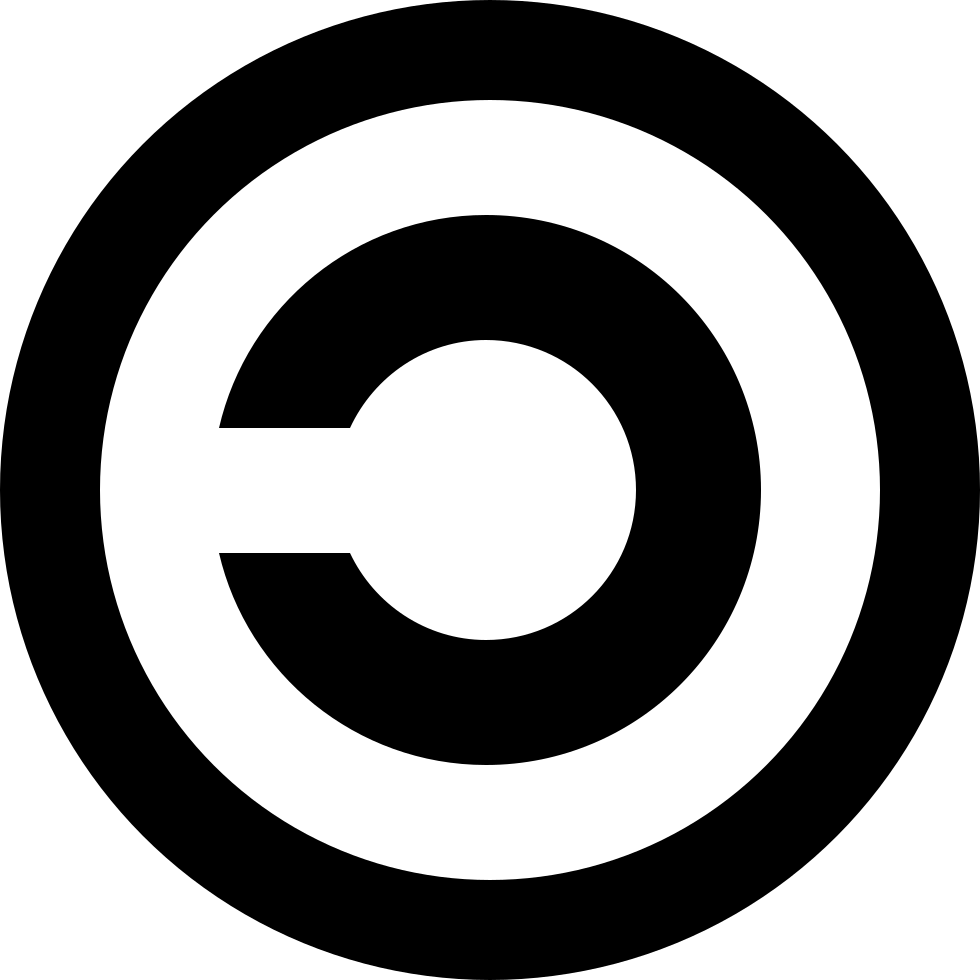
\includegraphics[width=1cm]{Copyleft.svg}
        \else
            
\includegraphics[width=1cm]{Copyleft.eps}
        \fi

Copyright (c) 2011-2012  Laurent Claessens,

Permission is granted to copy, distribute and/or modify this document under the terms of the \href{http://www.gnu.org/licenses/fdl-1.3.html}{GNU Free Documentation License}, Version 1.3 or any later version published by the Free Software Foundation; with no Invariant Sections, no Front-Cover Texts, and no Back-Cover Texts. A copy of the license is included in the section entitled ``GNU Free Documentation License''.

% Ajouter ici l'ISBN. Pour les révisions, mettre un nouvel ISBN et indiquer que c'est une révision.
% Pour l'ISBN:
% Copier tout dans un nouveau répertoire
% Créer une nouvelle branche git
% Coder en dur la date (càd enlever \today)
% Changer la licence vers non modifiable, copiable, et ajouter un lien vers la
%   version modifiable.

% http://www.bnf.fr/fr/professionnels/s_informer_obtenir_isbn/s.qu_est_ce_que_isbn.html

% TODO: écrire le README.txt

\end{center}

\clearpage



\tableofcontents

% This is part of Mes notes de mathématique
% Copyright (c) 2011-2012
%   Laurent Claessens
% See the file fdl-1.3.txt for copying conditions.

%+++++++++++++++++++++++++++++++++++++++++++++++++++++++++++++++++++++++++++++++++++++++++++++++++++++++++++++++++++++++++++
\section{Avertissement}
%+++++++++++++++++++++++++++++++++++++++++++++++++++++++++++++++++++++++++++++++++++++++++++++++++++++++++++++++++++++++++++

Ceci sont des notes «prises au vol» de certains de mes cours pour l'agrégation. Aucune garantie. Merci de me signaler toute faute ou remarque. En particulier je serais content que quelqu'un me donne un avis sur le points suivants :
\begin{enumerate}
    \item
        L'énoncé et la démonstration de la proposition \ref{PropNsLqWb}.
    \item
        Où trouver une preuve de la proposition \ref{PropKZDqTR} sur le supplémentaire topologique ?
    \item
        La preuve du théorème \ref{ThoJsBKir}.
    \item
        La preuve du lemme \ref{LemjXywjH}.
    \item
        La preuve du théorème de Fredholm \ref{ThoagJPZJ}.
    \item
        La preuve du lemme \ref{LemooynkH}.
    \item
        La partie «unicité» du théorème \ref{ThokUUlgU}.
    \item
        La preuve de la proposition \ref{PropRZCKeO}.
    \item
        L'inversion entre la somme et l'intégrale de l'équation \eqref{EqXSgZGw}.
    \item
        Si vous connaissez des exemples ou des contre-exemples intéressants à propos de quoi que ce soit, je suis toujours preneur.
\end{enumerate}

Une version avec ISBN de ce document est en préparation afin qu'il soit acceptable comme livre aux oraux de l'agrégation \ldots j'y travaille et on verra comment les choses vont évoluer.

%+++++++++++++++++++++++++++++++++++++++++++++++++++++++++++++++++++++++++++++++++++++++++++++++++++++++++++++++++++++++++++
\section{Auteurs, contributeurs et remerciements}
%+++++++++++++++++++++++++++++++++++++++++++++++++++++++++++++++++++++++++++++++++++++++++++++++++++++++++++++++++++++++++++

Le principal auteur et metteur en \LaTeX\ de ce document est votre serviteur, Laurent Claessens.

Les personnes qui ont du code \LaTeX\ dans ce document :
\begin{enumerate}
    \item
        Nicolas Richard et Ivik Swan pour les parties des exercices et rappels de calcul différentiel et intégral (Université libre de Bruxelles, 2003-2004) qui leur reviennent.
    \item
        Pierre Bieliavsky pour les énoncés d'analyse numérique (MAT1151 à Louvain la Neuve 2009-2010)
    \item
        Jonathan Di Cosmo pour certaines corrections de MAT1151
\end{enumerate}

Autres sources et remerciements :
\begin{enumerate}
    \item
        Tous les contributeurs du wikipédia francophone (et aussi un peu l'anglophone) doivent être remerciés. J'en ai pompé des quantités astronomiques; des articles utilisés sont cités à divers endroits du texte, mais ce n'est absolument pas exhaustif. Il n'y a à peu près pas un résultat important de ces notes dont je n'aie pas lu la page Wikipédia, et souvent plusieurs pages connexes.
    \item
        Des centaines de profs qui ont mis leurs polys sur internet. Des dizaines d'entre eux (et entre elles) ont des sites dédiés à l'agrégation. Ils sont cités en bibliographie aux endroits où ils sont utilisés. Merci à toutes et à tous d'avoir codé et publié.
    \item
        Le forum usenet de math, en particulier pour la construction des corps fini dans la fil «Vérifier qu'un polynôme est primitif» initié le 20 décembre 2011.
\end{enumerate}

%+++++++++++++++++++++++++++++++++++++++++++++++++++++++++++++++++++++++++++++++++++++++++++++++++++++++++++++++++++++++++++
					\section*{Ces notes sont les vôtres !}
%+++++++++++++++++++++++++++++++++++++++++++++++++++++++++++++++++++++++++++++++++++++++++++++++++++++++++++++++++++++++++


Il y a encore certainement des erreurs, des fautes de frappe et des choses pas claires. Je compte sur vous (oui : toi !) pour me signaler toute imperfection (y compris d'orthographe).

Plus vous signalez de fautes, meilleure sera la qualité du texte, et plus les étudiants de l'année prochaine vous seront reconnaissants.

%Tiens, tant que j'y suis je vous demanderais de penser à la quantité d'argent que vous auriez dû dépenser pour obtenir un texte tel que celui-ci chez un éditeur «classique» qui vous interdirait la photocopie et la redistribution. Maintenant que vous y avez pensé, je vous donnerais bien mon numéro de compte, mais non. J'ai tapé ce texte sur mes heures de travail à l'université; j'ai donc déjà été payé par les contribuables belges et français.

%+++++++++++++++++++++++++++++++++++++++++++++++++++++++++++++++++++++++++++++++++++++++++++++++++++++++++++++++++++++++++++
\section{Contre Moodle, Icampus, Claroline, et autres «plateformes de travail collaboratif»}
%+++++++++++++++++++++++++++++++++++++++++++++++++++++++++++++++++++++++++++++++++++++++++++++++++++++++++++++++++++++++++++

Ces notes ne sont pas destinées à être publiées sur des plateformes telles que Moodle, Icampus ou autres Clarolines. Pourquoi ? parce que la licence FDL l'interdit implicitement en demandant de publier sur des sites \emph{ouverts}.

L'internet est un système décentralisé et ouvert : tout le monde peut s'y connecter, y publier et y lire. C'est pour l'instant la meilleure solution technique inventée par l'humanité pour la diffusion d'information. Des sites comme \href{http://gitorious.org}{gitorious} ou \href{http://wikipedia.org}{wikipedia} sont de \emph{vrais} système de travail collaboratif.

Les plateformes soi-disant collaboratives comme Moodle en sont la négation. L'essentiel de ce qu'apporte Moodle par rapport à un vrai site internet n'est absolument pas la possibilité de partager des information (ça on peut le faire via internet depuis des décennies), mais bien de \emph{restreindre} l'accès à l'information via un système de mot de passe.

Lorsqu'un moine copiste du onzième siècle mettait un manuscrit dans sa bibliothèque, le document était immédiatement consultable par une centaine de moines, et (quitte à faire le déplacement) par des milliers d'érudits. Un document posté sur Moodle touche une dizaine de personnes. Utiliser Moodle pour partager ses documents est donc une régression non pas par rapport à l'internet d'il y a vingt ans, non pas par rapport à l'imprimerie d'il y a cinq siècles, mais bien par rapport aux bibliothèques d'abbayes d'il y a mille ans !

Lorsqu'on parle de science, qu'on veut y apporter un document, une question ou une réponse, un minimum d'honnête intellectuelle, d'éthique du partage de savoir (sans laquelle la science n'existe pas) et peut être aussi de courage, est de parler publiquement. Se cacher derrière un mot de passe et ne permettre l'accès au savoir qu'à ses seuls amis triés sur le volet est une négation de l'esprit scientifique; Moodle est une version dégénérée, une maladie de l'internet.

La faute fondamentale qui fait utiliser Moodle pour partager des documents de mathématique est la perte de notion entre le privé et le public ainsi que la paresse qui consiste à vouloir intégrer tous les outils dans une même interface, voire utiliser les mêmes outils pour effectuer des tâches différentes. Lorsqu'on pose une question de math, c'est essentiellement public; lorsqu'on pose une question d'organisation d'un cours, c'est privé. Ce sont deux activités totalement différentes qui nécessitent deux types d'outils différents. Dans le premier cas, l'outil adapté est internet, dans le deuxième cas, l'outil adapté est Moodle. Vouloir utiliser la même interface pour les deux est n'avoir fondamentalement pas compris le sens de l'internet et son utilité en tant que «outil de l'information».

{\tiny Cela dit c'est pratique pour discuter des horaires des cours ou s'échanger des informations pratiques qui n'ont pas à être publiques.}

%+++++++++++++++++++++++++++++++++++++++++++++++++++++++++++++++++++++++++++++++++++++++++++++++++++++++++++++++++++++++++++
\section{Instructions pour les examens et interrogations}
%+++++++++++++++++++++++++++++++++++++++++++++++++++++++++++++++++++++++++++++++++++++++++++++++++++++++++++++++++++++++++++

Ceci sont des conseils généraux que nous vous conseillons de suivre dans toutes les matières.
\begin{description}
    \item[numéroter] Numérotez clairement toutes les questions. Si votre réponse prend plus d'une page, écrivez «suite au verso», «suite à l'intercalaire \( n\)» etc. À l'endroit où la réponse continue, écrivez «question \( n\), suite».

    \item[vérifiez] Certaines erreurs sont faciles à détecter. Par exemple
        \begin{enumerate}
            \item
                les aires et volumes sont positifs;
            \item
                une intégrale \emph{définie} qui contient «\( dx\)» ne peut pas contenir de \( x\) dans la réponse;

            \item
                en physique et en chimie, les unités doivent être cohérentes : si la réponse est une énergie, vous devez avoir des joules (\unit{\square\metre\kilo\gram\per\square\second}).

        \end{enumerate}
    \item[votre nom] Écrivez votre nom et votre numéro de carte d'étudiant.

    \item[les faciles d'abord] Lisez d'abord toutes les questions avant de répondre. Commencez par les questions faciles.

    \item[justifier] Justifiez vos réponses. N'hésitez pas à écrire des phrases complètes : sujet, verbe, complément. N'abusez pas des symboles dont vous ignorez la signification :
        \begin{enumerate}
            \item
                «\( \Leftrightarrow\)» signifie «si et seulement si», et non «la suite de mon calcul»;
            \item

                «\( \nexists\)» signifie «il n'existe pas», et non «n'existe pas» ou «n'est pas défini».
        \end{enumerate}

    \item[ne pas passer en force] Si vous savez que votre réponse est fausse, mais vous ne savez pas la corriger, écrivez sur votre feuille «cette réponse est fausse pour telle raison, mais je ne sais pas comment corriger». Ne comptez pas sur une inattention du correcteur. En science, affirmer un fait que vous savez être faux s'appelle de la falsification; c'est déontologiquement inacceptable. De la même façon, si vous copiez sur votre voisin\footnote{Indépendamment que c'est sans doute interdit par le règlement; vérifiez avant.}, vous êtes priés de le citer : on ne s'approprie pas le travail d'autrui.

    \item[approximations numériques] Lorsque vous voulez écrire une approximation numérique, réfléchissez au sens de ce que vous allez écrire. En mathématique, ça n'a presque jamais de sens d'écrire une approximation parce que vous ne savez pas dans quel contexte votre calcul pourra être utilisé. Si vous laissez deux décimales à \( \pi\) pour calculer le volume d'eau dans votre piscine gonflable, ça fera l'affaire; si c'est pour calculer la masse du Higgs ou pour mettre un satellite autour de Mars, vous perdez plusieurs millions d'euros.

        En sciences naturelles (physique, chimie ou autres), vous pouvez donner des approximations numériques de façon circonstanciée. Demandez à votre prof de labo.

    \item[orthographe] Sans être obligatoire, ça ne fait jamais de mal. Surtout si le français est votre langue maternelle.
    \item[santé] Mangez des fruits et des légumes de saisons. Choisissez des producteurs locaux qui n'utilisent pas d'engrais synthétisés à base de pétrole. De toutes façons \href{http://www.energybulletin.net/node/51306}{vous n'avez pas le choix}.

\end{description}

%+++++++++++++++++++++++++++++++++++++++++++++++++++++++++++++++++++++++++++++++++++++++++++++++++++++++++++++++++++++++++++
\section{Propagande : utilisez un ordinateur !}
%+++++++++++++++++++++++++++++++++++++++++++++++++++++++++++++++++++++++++++++++++++++++++++++++++++++++++++++++++++++++++++

Si vous faites des exercices supplémentaires et que vous voulez des corrections, n'oubliez pas que vous avez un ordinateur à disposition. De nos jours, les ordinateurs sont capables de calculer à peu près tout ce qui se trouve dans vos cours de math\footnote{Avec une notable exception pour les limites à deux variables.}.

D'ailleurs, je te rappelle que nous sommes est déjà largement dans le vingt et unième siècle et que tu te destines à une carrière professionnelle dans laquelle tu auras des calculs à faire; si tu n'es pas encore capable d'utiliser un ordinateur pour faire ces calculs, il est temps de combler cette lacune.

%---------------------------------------------------------------------------------------------------------------------------
\subsection{Lancez-vous dans Sage}
%---------------------------------------------------------------------------------------------------------------------------

Le logiciel que je vous propose est \href{http://www.sagemath.org}{Sage}. Pour l'utiliser, il n'est même pas nécessaire de l'installer sur votre ordinateur~: il tourne en ligne, directement dans votre navigateur.

\begin{enumerate}

	\item
		Aller sur \href{http://www.sagenb.org}{http://www.sagenb.org}
	\item
		Créer un compte
	\item
		Créer des feuilles de calcul et amusez-vous !!

\end{enumerate}

Il y a beaucoup de \href{http://lmgtfy.com/?q=sage+documentation}{documentation} sur le \href{http://www.sagemath.org}{site officiel}\footnote{\href{http://www.sagemath.org}{http://www.sagemath.org}}.

Si vous comptez utiliser régulièrement ce logiciel, je vous recommande \emph{chaudement} de \href{http://mirror.switch.ch/mirror/sagemath/index.html}{l'installer} sur votre ordinateur. Ce logiciel étant distribué sous licence GPL, vous ne devez ni payer ni vous procurer de codes.

%---------------------------------------------------------------------------------------------------------------------------
\subsection{Exemples de ce que Sage peut faire pour vous}
%---------------------------------------------------------------------------------------------------------------------------

Voici une liste absolument pas exhaustive de ce que Sage peut faire pour vous, avec des exemples. 
\begin{enumerate}

	\item
		Calculer des limites de fonctions, voir l'exercice \ref{exoINGE11140028},

	\item
		D'autres limites et tracer des fonctions, voir l'exercice \ref{exoINGE11140031}.
	\item
		Calculer des dérivées, voir exercice \ref{exo0013}.
	\item
		Calculer des dérivées partielles de fonctions à plusieurs variables, voir exercice \ref{exoFoncDeuxVar0002}.
	\item
		Calculer des primitives, voir certains exercices \ref{exo0017}
	\item

		Résoudre des systèmes d'équations linéaires. Lire \href{http://www.sagemath.org/doc/constructions/linear_algebra.html#solving-systems-of-linear-equations}{la documentation} est ce qui fait la différence entre l'être humain et le non scientifique. Voir les exercices  \ref{exoINGE1121La0016} et \ref{exoINGE1121La0010}.

	\item
		Tout savoir d'une forme quadratique, voir exercice \ref{exoINGE1121La0018}.
	\item
		Calculer la matrice Hessienne de fonctions à deux variables, déterminer les points critiques, déterminer le genre de la matrice Hessienne aux points critiques et écrire extrema de la fonctions (sous réserve d'être capable de résoudre certaines équations), voir les exercices \ref{exoFoncDeuxVar0029} et \ref{exoFoncDeuxVar0028}.
	\item
		Lorsqu'il y a une infinité de solutions, Sage vous l'indique avec des paramètres (ne fonctionne hélas pas avec les fonctions trigonométriques), voir l'exercice \ref{exoDerrivePartielle-0007}.


	\item
		Calculer des dérivées symboliquement, voir exercice \ref{exoDerive-0002}.
	\item
		Calculer des approximations numériques comme dans l'exercice \ref{exoOutilsMath-0028}.
    \item
        Calculer dans un corps de polynômes modulo comme \( \eF_p[X]/P\) où \( P\) est un polynôme à coefficients dans \( \eF_p\). Voir l'exemple \ref{ExemWUdrcs}.
	\item
        Tracer des courbes en trois dimensions, voir exemple \ref{ExempleTroisDxxyy}. Notez que pour cela vous devez installer aussi le logiciel Jmol. Pour Ubuntu\footnote{Pour les autres, je ne sais pas, mais je laisserai jouer l' adage «Windows c'est facile». Quant aux utilisateurs d'OS «alternatifs» comme Hurd ou BSD ben heu \ldots} c'est dans le paquet \info{icedtea6-plugin}.
\end{enumerate}

Sage peut toutefois vous induire en erreur si vous n'y prenez pas garde parce qu'il sait des choses en mathématique que vous ne savez pas. Par conséquent il peut parfois vous donner des réponses (mathématiquement exactes) auxquelles vous ne vous attendez pas. Voir page \ref{PgpXBuBh}.

%+++++++++++++++++++++++++++++++++++++++++++++++++++++++++++++++++++++++++++++++++++++++++++++++++++++++++++++++++++++++++++
%\section{Propagande : n'utilisez pas votre calculatrice}
%+++++++++++++++++++++++++++++++++++++++++++++++++++++++++++++++++++++++++++++++++++++++++++++++++++++++++++++++++++++++++++

%D'abord, l'expérience montre que la majorité des fois qu'un étudiant sort sa calculatrice, c'est pour faire un calcul inutile, et le plus souvent la calculatrice fournit un résultat faux. Étant en 2012, vous ne devriez pas vous contenter de vos calculatrices qui coûtent un os, qui n'ont pas de puissance de calcul, qui ont une définition d'écran ridicule et en noir et blanc. Remarquez que votre GSM (et a forciori vos minis trucs qui se connectent a internet) sont considérablement plus puissants que ces vieilleries; ils ont un meilleur écran.


\part{Mes notes d'agrégation}

\chapter{Théorie des groupes}
Nous allons suivre dans un premier temps \cite{Kropholler}.


\begin{definition}
    Soit \( G\) un groupe. Le \defe{centralisateur}{centralisateur} de \( H\subset G\) est 
    \begin{equation}
        \mZ_G(H)=\{ g\in G\tq hg=gh\,\forall h\in h\}
    \end{equation}
    Si \( H\) est un sous groupe, son \defe{centralisateur}{centralisateur} est
    \begin{equation}
        N_G(H)=\{ g\in G\tq gH=Hg \}.
    \end{equation}
\end{definition}

\begin{definition}
    Un sous groupe \( N\) de \( G\) est \defe{normal}{normal!sous groupe} si pour tout \( g\in G\) et pour tout \( n\in N\), \( gng^{-1}\in N\). Autrement dit lorsque \( gNg^{-1}\subset N\). Lorsque \( N\) est normal dans \( G\) nous noterons \( N\normal G\)\nomenclature[]{\(N \normal G\)}{\( N\) est normal dans \( G\)}.
\end{definition}

\begin{proposition}
    Soit \( N\) un sous groupe de \( G\). Les propriétés suivantes sont équivalentes :
    \begin{enumerate}
        \item
            \( gNg^{-1}\subseteq N\) pour tout \( g\in G\),
        \item
            \( gNg^{-1}= N\) pour tout \( g\in G\),
        \item
            \( gN=Ng\) pour tout \( g\in G\),
        \item
            \( N\) est une union de classes de conjugaison de \( G\),
        \item
            \( N\) est normal.
    \end{enumerate}
\end{proposition}

\begin{definition}
    Soit \( g\in G\) et \( n\in \eZ\). Nous définissons \( g^n\) par
    \begin{enumerate}
        \item
            \( g^0=e\) et \( g^n=gg^{n-1}\) si \( n\) est positif.
        \item
            si \( n<0\), nous posons \( g^n=(g^{-1})^{-n}\).
    \end{enumerate}
\end{definition}

\begin{definition}
    Si \( G\) est un groupe, l'\defe{ordre}{ordre!d'un groupe} est la cardinalité de \( G\) et est noté \( | G |\). L'\defe{ordre}{ordre!élément} d'un élément \( g\) de \( G\) est le naturel
    \begin{equation}
        \min\{ n\in\eN\tq g^n=e \}.
    \end{equation}
    Si le minimum n'existe pas, nous disons que l'ordre de \( g\) est infini.
\end{definition}

%+++++++++++++++++++++++++++++++++++++++++++++++++++++++++++++++++++++++++++++++++++++++++++++++++++++++++++++++++++++++++++
\section{Théorèmes d'isomorphismes}
%+++++++++++++++++++++++++++++++++++++++++++++++++++++++++++++++++++++++++++++++++++++++++++++++++++++++++++++++++++++++++++

Si \( G\) est un groupe et si \( N\) est un sous groupe normal, alors l'ensemble \( G/N\) a une structure de groupe et la projection canonique \( \pi\colon G\to G/N\) est un homomorphisme surjectif de noyau~\( N\).

\begin{theorem}[premier théorème d'isomorphisme]
    Soit \( \theta\colon G\to H\) un homomorphisme de groupe. Alors
    \begin{enumerate}
        \item
            \( \Kernel\theta\) est normal dans \( G\),
        \item
            \( \Image \theta\) est un sous groupe de \( H\)
        \item
            nous avons un isomorphisme naturel
            \begin{equation}
                G/\Kernel\theta\simeq \Image\theta
            \end{equation}
    \end{enumerate}
\end{theorem}

\begin{proof}
    \begin{enumerate}
        \item
        \item
        \item
            Si \( [g]\) représente la classe de \( g\) dans \( G/\Kernel\theta\), l'isomorphisme est donné par \( \varphi[g]=\theta(g)\).
    \end{enumerate}
\end{proof}


\begin{theorem}[Deuxième théorème d'isomorphisme]
    Soient \( H\) et \( N\) deux sous groupes de \( G\) et supposons que \( N\) soit normal. Alors
    \begin{enumerate}
        \item
            \( NH=HN\) est un sous groupe
        \item
            \( N\normal NH\)
        \item
            \( N\cap H\normal H\)
        \item
            nous avons un isomorphisme
            \begin{equation}
                NH/N\simeq H/H\cap N.
            \end{equation}
    \end{enumerate}
\end{theorem}

\begin{proof}
    \begin{enumerate}
        \item
        \item
        \item
        \item
            Il faut d'abord remarquer que \( H\) et \( N\) étant des groupes et le produit \( NH\) étant un groupe, nous avons \( NH=HN\). Soit le morphisme injectif
            \begin{equation}
                \begin{aligned}
                    j\colon H&\to HN \\
                    h&\mapsto h
                \end{aligned}
            \end{equation}
            et la surjection canonique
            \begin{equation}
                \sigma\colon HN\to HN/N 
            \end{equation}
            Nous considérons ensuite l'application composée
            \begin{equation}
                \begin{aligned}
                    f\colon H&\to HN/N \\
                    h&\mapsto hN. 
                \end{aligned}
            \end{equation}
            L'application \( f\) est surjective parce que l'élément \( hnN\in HN/N\) est l'image de \( h\), étant donné que \( hnN=hN\).

            Le noyau de \( f\) est \( \Kernel f=H\cap N\). En effet si \( a\in H\cap N\), nous avons \( f(a)=\sigma(a)\in K\). Par conséquent \( H\cap N\subset \Kernel f\). D'autre part si \( h\in H\) vérifie \( h\in\Kernel f\), alors \( f(h)=hN=N\), ce qui est uniquement possible si \( h\in N\).

            Le premier théorème d'isomorphisme implique alors que \( H/\Kernel f\simeq \Image f\), c'est à dire
            \begin{equation}
                H/N\cap H\simeq HN/N.
            \end{equation}
    \end{enumerate}
\end{proof}

\begin{theorem}[Troisième théorème d'isomorphisme]
    Soient \( N\) et \( M\) deux sous groupes normaux de \( G\) avec \( M\subset N\). Alors \( N/M\) est normal dans \( G/M\) et
    \begin{equation}
        (G/M)/(N/M)\simeq G/N.
    \end{equation}
\end{theorem}

\begin{proof}
    Afin de montrer que \( N/M\) est normal dans \( G/M\), nous considérons \( g\in G\), \( nM\in N/M\) et nous calculons
    \begin{equation}
        gnMg^{-1}=gng^{-1}\underbrace{gMg^{-1}}_{=M}=\underbrace{gng^{-1}}_{\in N}M\in N/M.
    \end{equation}

    Pour prouver l'isomorphisme nous considérons le morphisme
    \begin{equation}
        \begin{aligned}
            \varphi\colon G/M&\to G/N \\
            gM&\mapsto gN. 
        \end{aligned}
    \end{equation}
    C'est surjectif et le noyau est \( N/M\) parce que \( \varphi(gM)=N\) uniquement si \( g\in N\). Nous pouvons appliquer le premier théorème d'isomorphisme à \( \varphi\) en écrivant
    \begin{equation}
        (G/M)/\Kernel \varphi\simeq\Image \varphi,
    \end{equation}
    c'est à dire
    \begin{equation}
        (G/M)/(N/M)\simeq G/N.
    \end{equation}
\end{proof}

%+++++++++++++++++++++++++++++++++++++++++++++++++++++++++++++++++++++++++++++++++++++++++++++++++++++++++++++++++++++++++++
\section{Indice d'un sous groupe}
%+++++++++++++++++++++++++++++++++++++++++++++++++++++++++++++++++++++++++++++++++++++++++++++++++++++++++++++++++++++++++++

Soit \( G\) un groupe fini et \( H\), un sous groupe. L'\defe{indice}{indice} de \( H\) dans \( G\) est le nombre \( | G |/| H |\), souvent noté \( | G:H |\). Le théorème de Lagrange dira en particulier que l'indice est toujours un nombre entier.

\begin{theorem}[Théorème de Lagrange]\index{théorème!Lagrange}
    Soit \( H\) un sous groupe du groupe fini \( G\). Alors \( | H |\) divise \( | G |\) et les trois nombres suivants sont égaux :
    \begin{enumerate}
        \item
            le nombre de classes de \( H\) à gauche,
        \item
            le nombre de classes de \( H\) à droite,
        \item
            l'indice de \( H\) dans \( G\).
    \end{enumerate}
\end{theorem}

\begin{proof}
    Nous commençons par montrer que les classes de \( H\) ont toutes les même nombre d'éléments que \( H\). En effet pour chaque \( g\in G\) nous avons la bijection
    \begin{equation}
        \begin{aligned}
            \varphi\colon H&\to gH \\
            h&\mapsto gh. 
        \end{aligned}
    \end{equation}
    L'injectivité de \( \varphi\) est le fait que \( gh=gh'\) implique \( h=h'\). La surjectivité est par définition de la classe.
\end{proof}
<++>


\chapter{Anneaux et corps}
%+++++++++++++++++++++++++++++++++++++++++++++++++++++++++++++++++++++++++++++++++++++++++++++++++++++++++++++++++++++++++++
\section{Généralités}
%+++++++++++++++++++++++++++++++++++++++++++++++++++++++++++++++++++++++++++++++++++++++++++++++++++++++++++++++++++++++++++

Source : \cite{Tauvel}.

\begin{definition}
    Un \defe{anneau}{anneau} est un triple \( (A,+,\cdot)\) avec les conditions
    \begin{enumerate}
        \item
            \( (A,+)\) est un groupe abélien. Nous notons \( 0\) le neutre.
        \item
            La multiplication est associative et nous notons \( 1\) le neutre
        \item
            La multiplication est distributive par rapport à l'addition.
    \end{enumerate}
\end{definition}

\begin{remark}
    Un anneau est ce qu'on appelle «\emph{ring}» en anglais.
\end{remark}


Soit \( X\) un ensemble et $A$ un anneau. Nous considérons \( \Fun(X,A)\)\nomenclature[A]{\( \Fun(X,Y)\)}{les applications de \( X\) vers \( Y\)} l'ensemble des applications \( X\to A\). Cet ensemble devient un anneau avec les définitions
\begin{subequations}
    \begin{align}
        (f+g)(x)=f(x)+g(x)\\
        (fg)(x)=f(x)g(x).
    \end{align}
\end{subequations}
Cela est la \defe{structure canonique}{structure d'anneau canonique} d'anneau sur \( \Fun(X,A)\).

Le \defe{centralisateur}{centralisateur} de \( x\in A\) dans \( A\) est l'ensemble
\begin{equation}
    \{ y\in A\tq xy=yx \},
\end{equation}
le \defe{centre}{centre} de \( A\) est
\begin{equation}
    \{ y\in A\tq xy=yx\forall x\in A \}.
\end{equation}
Un élément \( a\neq 0\) est un \defe{diviseur de zéro à gauche}{diviseur!de zéro} si il existe \( x\neq 0\) tel que $xa=0$. L'élément \( a\) est un diviseur de zéro \defe{à droite}{diviseur!de zéro à droite} si il existe \( b\) tel que \( ab=0\). Un anneau est \defe{intègre}{intègre!anneau}\index{anneau!intègre} si il est non nul et ne possède pas de diviseurs de zéro.

\begin{example}
    L'ensemble \( \eZ\) avec les opérations usuelles est un anneau intègre.
\end{example}

Un élément \( a\in A\) est \defe{régulier à droite}{régulier à droite} \( ba=0\) implique \( b=0\). Il est régulier ) gauche si \( ab=0\) implique \( b=0\).

L'ensemble \( U(A)\)\nomenclature[A]{\( U(A)\)}{ensemble des inversibles} des éléments inversibles de \( A\) est un groupe pour la multiplication. Nous notons \( A^*=A\setminus\{ 0 \}\).

\begin{lemma}
    Si \( a\) et \( b\) commutent, nous avons la formule
    \begin{equation}        \label{Eqarpurmkbk}
        a^{r+1}-b^{r+1}=(a-b)(\sum_ka^{r-k}b^k).
    \end{equation}
\end{lemma}

\begin{proposition}
    Si \( a\) est un élément nilpotent de l'anneau \( A\), alors \( 1-a\) est inversible. Si \( a\) est nilpotent non nul, alors il est diviseur de zéro.
\end{proposition}

\begin{proof}
    Soit \( n\) le minimum tel que \( a^n=0\). En vertu de la formule \eqref{Eqarpurmkbk} nous avons
    \begin{equation}
        1=1-a^n=(1-a)(1+a+\ldots+a^{n-1})=(1+a+\ldots+a^{n-1})(1-a).
    \end{equation}
    La somme \( 1+a+\ldots+a^{n-1}\) est donc un inverse de \( (1-a)\).
\end{proof}

\begin{definition}
    Si \( A\) et \( B\) sont des anneaux, un \defe{morphisme}{morphisme!d'anneaux} est une application \( f\colon A\to B\) telle que pour tout \( x,y\in A\) nous ayons
    \begin{enumerate}
        \item
            \( f(x+y)=f(x)+f(y)\)
        \item
            \( f(xy)=f(x)f(y)\)
        \item
            \( f(1)=1\)
    \end{enumerate}
\end{definition}

Si \( f\) est un morphisme, nous avons \( f(0)=0\) et \( f(x)^{-1}=f(x^{-1})\).

%+++++++++++++++++++++++++++++++++++++++++++++++++++++++++++++++++++++++++++++++++++++++++++++++++++++++++++++++++++++++++++
\section{Idéaux dans des anneaux}
%+++++++++++++++++++++++++++++++++++++++++++++++++++++++++++++++++++++++++++++++++++++++++++++++++++++++++++++++++++++++++++

\begin{definition}
    Un sous ensemble \( B\subset A\) d'un anneau est un \defe{sous anneau}{sous anneau} si
    \begin{enumerate}
        \item
            \( 1\in B\)
        \item
            \( B\) est un sous groupe pour l'addition
        \item
            \( B\) est stable pour la multiplication.
    \end{enumerate}
    Un sous ensemble \( I\subset A\) est un \defe{idéal}{idéal!dans un anneau} à gauche si
    \begin{enumerate}
        \item
            \( I\) est un sous groupe pour l'addition
        \item
            si \( x\in I\) et \( a\in A\), alors \( ax\in I\).
    \end{enumerate}
\end{definition}

Lorsqu'un ensemble est idéal à gauche et à droite, nous disons que c'est un \defe{idéal bilatère}{idéal!bilatère}. Lorsque nous parlons d'idéal sans précisions, nous parlons d'idéal bilatère.

\begin{remark}
    Un idéal n'est pas toujours un anneau parce que l'identité pourrait manquer. Un idéal qui contient l'identité est l'anneau complet.
\end{remark}

\begin{example}
    L'ensemble \( 2\eZ\) est un idéal de \( \eZ\). Tous les idéaux de \( \eZ\) sont de la forme \( n\eZ\). En effet en vertu de la proposition \ref{PropSsgpZestnZ}, les seule sous groupes de \( \eZ\) (en tant que groupe additif) sont les \( n\eZ\).
\end{example}

Soit \( A\), un anneau, \( I\) un idéal bilatère de \( A\). Nous considérons la relation d'équivalence \( x\sim y\) si et seulement si \( x-y\in I\). Dans ce cas, le quotient
\begin{equation}
    A/\sim=A/I
\end{equation}
est un anneau appelé \defe{anneau quotient}{anneau!quotient par un idéal}. La surjection \( A\to A/I\) est un morphisme.

\begin{proposition}
    Soient \( A\) et \( B\) des anneaux et un homomorphisme \( f\colon A\to B\). Nous considérons l'injection canonique \( j\colon f(A)\to B\) et la surjection canonique \( \phi\colon A\to A/\ker f\). Alors il existe un unique isomorphisme
    \begin{equation}
        \tilde f \colon A/\ker f\to f(A)
    \end{equation}
    tel que \( f=j\circ\tilde f\circ\phi\).

    \begin{equation}
        \xymatrix{%
        A \ar[r]^{f}\ar[d]_{\phi}        &   B\ar[d]^{j}\\
           A/\ker f \ar[r]_{\tilde f}   &   f(A)\subset B
           }
    \end{equation}
\end{proposition}

\begin{proposition}
    Soit \( I\), un idéal de \( A\) et \( \phi\colon A\to A/I\) la surjection canonique. Les idéaux de \( A/I\) sont les \( \phi(J)\) où \( J\) est un idéal de \( A\) contenant \( I\)
\end{proposition}

\begin{proof}
    Si \( I\subset J\) et si \( J \) est un idéal de \( A\), alors \( \phi(J)\) est un idéal dans \( A/I\). En effet un élément de \( \phi(J)\) est de la forme \( \phi(j)\) et un élément de \( A/I\) est de la forme \( \phi(i)\). Leur produit vaut
    \begin{equation}
        \phi(i)\phi(j)=\phi(ij)\in\phi(J).
    \end{equation}
    
    Soit maintenant \( K\), un idéal dans \( A/I\). Soit \( J=\phi^{-1}(K)\). Étant donné qu'un idéal doit contenir \( 0\) (parce qu'un idéal est un groupe pour l'addition), \( [0]\in K\) et par conséquent \( I\subset\phi^{-1}(K)\).
\end{proof}

\begin{corollary}
    Les quotients de \( \eZ\) sont \( \eZ_n\)
\end{corollary}

\begin{proof}
    Nous avons déjà vu que les seuls idéaux de \( \eZ\) sont les \( n\eZ\).
\end{proof}

\begin{proposition}     \label{PropZpintssiprempUzn}
    Soit \( n\geq 2\) un entier et \( \phi\colon \eZ\to \eZ_n\), la surjection canonique. Nous noterons \( \tilde a=\phi(a)\). Alors
    \begin{equation}
        U(\eZ_n)=\phi(P_n)=\{ \tilde x\tq 0\leq x\leq n\tq\pgcd(x,n)=1 \}.
    \end{equation}
    où \( P_n\) est l'ensemble décrit par l'équation \eqref{EqDefPnEntierldeost}. En particulier, \( \Card\big( U(\eZ_n) \big)=\varphi(n)\).

    L'anneau \( \eZ_n\) est intègre si et seulement si \( n\) est premier.
\end{proposition}

\begin{proof}
    Soit \( 0\leq x\leq n\) tel que \( \pgcd(x,n)=1\). Il existe donc \( p,q\in\eZ\) tels que \( px+qn=1\). En passant aux classes,
    \begin{equation}
        \tilde p\tilde x=\tilde 1,
    \end{equation}
    donc \( \tilde p\) est l'inverse de \( \tilde x\). Cela prouve que \( \phi(P_n)\subset U(\eZ_n)\).

    Nous prouvons maintenant l'inclusion inverse. Soit \( \tilde x\) et \( \tilde y\) inverses l'un de l'autre : $\tilde x\tilde y=\tilde 1$. Il existe donc \( q\in\eZ\) tel que \( xy-qn=1\), ce qui prouve que \( \pgcd(x,n)=1\).

    Si \( n\) est premier, tous les éléments de \( \eZ_n\) sont inversibles parce que tous les éléments rentrent dans \( \phi(P_n)\). Donc \( \eZ_n\) est intègre.

    Si \( n\) n'est pas premier, il existe \( p,q\in\eN^*\) tels que \( pq=n\). Dans ce cas au niveau des classes nous avons \( \tilde p\tilde q=0\) avec \( \tilde p\neq 0\neq\tilde q\), ce qui montre que \( \eZ_n\) a des diviseurs de zéro et n'est pas intègre.
\end{proof}

%---------------------------------------------------------------------------------------------------------------------------
\subsection{Caractéristique}
%---------------------------------------------------------------------------------------------------------------------------

L'application 
\begin{equation}
    \begin{aligned}
        \mu\colon \eZ&\to A \\
        n&\mapsto n\cdot 1_A 
    \end{aligned}
\end{equation}
est un morphisme d'anneaux. Le noyau de \( \mu\) étant un sous groupe de \( \eZ\), il existe un et un seul \( p\in\eZ\) tel que \( \ker\mu=p\eZ\). Ce \( p\) est la \defe{caractéristique}{caractéristique!d'un anneau} de \( A\).

\begin{lemma}
    Si \( A\) est de caractéristique nulle, alors \( A\) est infini.
\end{lemma}

\begin{proof}
    En effet, \( \ker\mu=0\) implique que \( n1_A\neq  m1_A\) et par conséquent \( A\) est infini.
\end{proof}

\begin{lemma}
    Si \( p\) est la caractéristique de l'anneau \( A\), alors nous avons l'isomorphisme d'anneaux
    \begin{equation}
         \eZ 1_A\simeq\eZ/p\eZ.
    \end{equation}
\end{lemma}

\begin{proof}
    L'isomorphisme est donné par l'application \( n1_A\mapsto \phi(n)\) si \( \phi\) est la projection canonique \( \eZ\to \eZ_p\).
\end{proof}

\begin{lemma}
    La caractéristique d'un anneau intègre est zéro ou un nombre premier.
\end{lemma}

\begin{proof}
    Si \( A\) est intègre, alors \( \eZ 1_A\) est intègre (a fortiori), et \( \eZ_p\) est intègre parce qu'il est isomorphe à \( \eZ A_A\). Mais nous savons que \( \eZ_p\) est intègre si et seulement si \( p\) est premier (proposition \ref{PropZpintssiprempUzn}).
\end{proof}

\begin{theorem}[Théorème chinois]\index{théorème!chinois}
    Soit \( A\) un anneau commutatif, \( n\geq 2\), des éléments \( x_1,\ldots,x_n\) dans \( A\) et des idéaux \( I_1,\ldots,I_n\) tels que \( I_i+I_j=A\) pour tout \( i\neq j\).

    Alors il existe un \( x\in A\) tel que \( x-x_i\in I_i\) pour tout \( 1\les i\leq n\).
\end{theorem}

\begin{proof}
    Pour \( i\in\{ 1,\ldots,n \}\) nous notons \( J_i\) le produit \( J_i=\prod_{k\neq i}I_k\). Étant donné que chaque \( I_i\) est un idéal, nous avons \( I_k\in J_i\) lorsque \( i\neq k\).

    Soit \( i\) fixé, et considérons \( j\neq i\). Nous pouvons trouver \( a_j\in I_i\) et \( b_j\in I_j\) tel que \( a_j+b_j=1\). Nous avons alors
    \begin{equation}
        1=\prod_{j\neq i}(a_j+b_j).
    \end{equation}
    Par ailleurs \( I_i+J_i=A\) parce que \( J_i\) contient \( I_k\) avec \( k\neq i\) et \( I_i+I_k=A\). Nous pouvons donc prendre \( \alpha_i\in I_i\) et \( \beta_i\in J_i\) tels que
    \begin{equation}
        \prod_{j\neq i}(a_j+b_j)=\alpha_i+\beta_i.
    \end{equation}
    Nous considérons alors l'élément \( x=\beta_1x_1+\ldots+\beta_nx_n\) et nous avons
    \begin{subequations}
        \begin{align}
            x-x_&=(\beta_1-1)x_1+\beta_2x_n+\ldots+\beta_nx_n\\
            &=-\alpha_1x_1+\beta_2x_2+\ldots+\beta_nx_n.
        \end{align}
    \end{subequations}
    Mais \( \alpha_1\in I_1\) et tous les autres termes sont dans les \( J_i\) avec \( i\neq 1\). Par conséquent le tout est dans \( I_1\). Ici nous utilisons par exemple le fait que \( \beta_2\in J_2\subset I_1\) parce que les éléments de \( J_2\) sont des produits d'éléments dont un facteur est dans \( I_1\).
\end{proof}
<++>



\chapter{Espaces vectoriels}
% This is part of Mes notes de mathématique
% Copyright (c) 2011-2012
%   Laurent Claessens, Carlotta Donadello
% See the file fdl-1.3.txt for copying conditions.



%+++++++++++++++++++++++++++++++++++++++++++++++++++++++++++++++++++++++++++++++++++++++++++++++++++++++++++++++++++++++++++
\section{Espace vectoriel normé}
%+++++++++++++++++++++++++++++++++++++++++++++++++++++++++++++++++++++++++++++++++++++++++++++++++++++++++++++++++++++++++++

La valeur absolue est essentielle pour introduire les notions de limite et de continuité pour les fonctions d'une variable. En fait nous disons que la fonction $f\colon \eR\to \eR$ est continue au point $a$ lorsque pour tout $\varepsilon$, il existe un $\delta$ tel que
\begin{equation}
	| x-a |\leq\delta \Rightarrow | f(x)-f(a) |\leq \varepsilon.
\end{equation}
La quantité $| x-a |$ donne la «distance» entre $x$ et $a$; la définition de la continuité signifie que pour tout $\varepsilon$, il existe un $\delta$ tel que si $a$ et $x$ sont au plus à la distance $\delta$ l'un de l'autre, alors $f(x)$ et $f(a)$ ne seront éloigné au plus d'une distance $\varepsilon$.

La valeur absolue, dans $\eR$, nous sert donc à mesurer des distances entre les nombres. Les principales propriétés de la valeur absolue sont :
\begin{enumerate}

	\item
		$| x |=0$ implique $x=0$,
	\item
		$| \lambda x |=| \lambda | |x |$,
	\item
		$| x+y |\leq | x |+| y |$

\end{enumerate}
pour tout $x,y\in\eR$ et $\lambda\in\eR$.

Afin de donner une notion de limite pour les fonctions de plusieurs variables, nous devons trouver un moyen de définir les notion de <<taille>> d'un vecteur et de distance entre deux points de $\eR^n$, avec $n>1$. La notion de <<taille>> doit satisfaire propriétés analogues à celles de la valeur absolue. 

La premier notion de <<taille>> pour un vecteur de $\eR^2$ que nous vient à l'esprit est la longueur du segment entre l'origine et l'extrémité libre du vecteur. Cela peut être calculée à l'aide du théorème de Pythagore : 
\begin{equation}
  \textrm{taille de } (a,b) = \sqrt{a^2+b^2}.
\end{equation}
Nous pouvons introduire une la notion de distance entre les éléments de $\eR^2$ de façon similaire :
\begin{equation}
	d\big((a_x,a_y),(b_x,b_y)\big)=\sqrt{  (a_x-b_x)^2+(a_y-b_y)^2  }.
\end{equation}
Cette définition a l'air raisonnable; est-elle mathématiquement correcte ? Peut-elle jouer le rôle de la valeur absolue dans $\eR^2$ ? Est-elle la seule définitions possibles de <<taille>> et distance en $\eR^2$ ?  


%+++++++++++++++++++++++++++++++++++++++++++++++++++++++++++++++++++++++++++++++++++++++++++++++++++++++++++++++++++++++++++
\section{Normes et distances}\label{Sect_definition}
%+++++++++++++++++++++++++++++++++++++++++++++++++++++++++++++++++++++++++++++++++++++++++++++++++++++++++++++++++++++++++++

Nous voulons formaliser les notions de «taille» et de distance dans $\eR^n$, et plus généralement dans un espace vectoriel $V$ de dimension finie. Pour cela nous nous inspirons des propriétés de la valeur absolue.
\begin{definition}		\label{DefNorme}
	Soit $V$ un espace vectoriel réel. Une \defe{norme}{norme!définition} est une application $N\colon V\to \eR^+$ vérifiant les axiomes 
	\begin{enumerate}

		\item
			$N(0_V)=0$, et $N(x)=0$ implique $x=0_V$;
		\item\label{ItemDefNormeii}
			$N(\lambda x)=| \lambda |N(x)$ pour tout $\lambda\in\eR$ et $x\in V$;
		\item\label{ItemDefNormeiii}
			$N(x+y)\leq N(x)+N(y)$ pour tout $x,y\in V$. Cette propriété est appelée \defe{inégalité triangulaire}{inégalité!triangulaire}.
	\end{enumerate}
	Ici et dans la suite, $0_V$ désigne l'élément zéro de l'espace $V$.
\end{definition}
En prenant $\lambda=-1$ dans la propriété \ref{ItemDefNormeii}, nous trouvons immédiatement que $N(-x)=N(x)$.

\begin{proposition}		\label{PropNmNNm}
	Toute norme $N$ sur l'espace vectoriel $V$ vérifie l'inégalité
	\begin{equation}
		\big| N(x)-N(y) \big|\leq N(x-y)
	\end{equation}
	pour tout $x,y\in V$.
\end{proposition}
	
\begin{proof}
	Nous avons, en utilisant le point \ref{ItemDefNormeiii} de la définition \ref{DefNorme},
	\begin{subequations}
		\begin{align}
			N(x)&=N(x-y+y)\leq N(x-y)+N(y),	\label{subEqNNNxxyyya}\\
			N(y)&=N(y-x+x)\leq N(y-x)+N(x).	\label{subEqNNNxxyyyb}
		\end{align}
	\end{subequations}
	Supposons d'abord que $N(x)\geq N(y)$. Dans ce cas, en utilisant \eqref{subEqNNNxxyyya},
	\begin{equation}
		\big| N(x)-N(y) \big|=N(x)-N(y)\leq N(x-y)+N(y)-N(y)=N(x-y).
	\end{equation}
	Si par contre $N(x)\leq N(y)$, alors nous utilisons \eqref{subEqNNNxxyyyb} et nous trouvons
	\begin{equation}
		\big| N(x)-N(y) \big|=N(y)-N(x)\leq N(y-x)+N(x)-N(x)=N(y-x).
	\end{equation}
	Dans les deux cas, nous avons retrouvé l'inégalité annoncée.
\end{proof}
Cette proposition signifie aussi que
\begin{equation}	\label{EqNleqNNleqNvqlqbs}
	-N(x-y)\leq N(x)-N(y)\leq N(x-y).
\end{equation}

Afin de suivre une notation proche de celle de la valeur absolue, à partir de maintenant, la norme d'un vecteur $v$ sera notée $\| v\|$ au lieu de $N(v)$.
\begin{definition}		\label{DefEVNetDistance}
	Un espace vectoriel $V$ muni d'une norme est une \defe{espace vectoriel normé}{normé!espace vectoriel}, et on écrit $(V,\| . \|)$. La \defe{distance induite}{distance (d'une norme)} par la norme entre les points $a$ et $b$ de $V$ est le nombre $d(a,b)=\| a-b \|$.

	Si $A$ est une partie de $V$ et si $x\in V$, nous disons que la \defe{distance}{distance!point et ensemble} entre $A$ et $x$ est le nombre
	\begin{equation}		\label{EqdefDistaA}
		d(x,A)=\inf_{a\in A}d(x,a).
	\end{equation}
\end{definition}
%The result is on the figure \ref{LabelFigDistanceEnsemble}
\newcommand{\CaptionFigDistanceEnsemble}{La distance entre $x$ et $A$ est donnée par la distance entre $x$ et $p$. Les distances entre $x$ et les autres points de $A$ sont plus grandes que $d(x,p)$.}
\input{Fig_DistanceEnsemble.pstricks}

Il est possible de définir de nombreuses normes sur $\eR^n$. Citons en quelque unes. Les normes $\| . \|_{L^p}$ ($p\in\eN$) sont définies de la façon suivante :
\begin{equation}		\label{EqDeformeLp}
	\| x \|_{L^p}=\Big( \sum_{i=1}^n| x_i |^p\Big)^{1/p},
\end{equation}
pour tout $x=(x_1,\ldots,x_n)\in\eR^n$. Parmi ces normes, celles qui seront le plus souvent utilisées dans ces notes sont
\begin{equation}
	\begin{aligned}[]
		\| x \|_{L^1}&=\sum_{i=1}^n| x_i |,\\
		\| x \|_{L^2}&=\Big( \sum_{i=1}^n| x_i |^2 \Big)^{1/2}.
	\end{aligned}
\end{equation}
La norme $L^2$ est la \defe{norme euclidienne}{norme!euclidienne}. Nous définissons également la \defe{norme supremum}{norme!supremum} par
\begin{equation}
	\| x \|_{\infty}=\sup_{1\leq i\leq n}| x_i |.
\end{equation}
Nous admettons sans démonstration que les fonctions $\| . \|_{L^p}\colon \eR^n\to \eR^+$ sont bien des normes.

\newcommand{\CaptionFigDistanceEuclide}{La \emph{norme} euclidienne induit la \emph{distance} euclidienne. D'où son nom. Le point $C$ est construit aux coordonnées $(A_x,B_y)$.}
\input{Fig_DistanceEuclide.pstricks}

Soient $A=(A_x,A_y)$ et $B=(B_x,B_y)$ deux éléments de $\eR^2$. La distance\footnote{Ne pas confondre «distance» et «norme».} euclidienne entre $A$ et $B$ est donnée par $\| A-B \|_2$. En effet, sur la figure \ref{LabelFigDistanceEuclide}, la distance entre les points $A$ et $B$ est donnée par
\begin{equation}
	| AB |^2=| AC |^2+| CB |^2=| A_x-B_x |^2+| A_y-B_y |^2,
\end{equation}
par conséquent,
\begin{equation}
	| AB |=\sqrt{| A_x-B_x |^2+| A_y-B_y |^2}=\| A-B \|_2.
\end{equation}

\begin{remark}
	Si $A$, $B$ et $C$ sont trois points dans le plan $\eR^2$, alors l'inégalité triangulaire $| AB |\leq| AC |+| CB |$ est précisément la propriété \ref{ItemDefNormeiii} de la norme (définition \ref{DefNorme}). En effet l'inégalité triangulaire s'exprime de la façon suivante en terme de la norme $\| . \|_2$ :
	\begin{equation}	\label{EqNDeuxAmBNNdd}
		\| A-B \|_2\leq \| A-C \|_2+\| C-B \|_2.
	\end{equation}
	En notant $u=A-C$ et $v=C-B$, l'équation \eqref{EqNDeuxAmBNNdd} devient exactement la propriété de définition de la norme :
	\begin{equation}
		\| u+v \|_2\leq \| u \|_2+\| v \|_2.
	\end{equation}
	Ceci explique pourquoi cette propriété des norme est appelée «inégalité triangulaire».
\end{remark}

Les distances que nous avons vues jusqu'à présent sont des distances définies à partir d'une norme. La définition suivante donne une notion générale de distance sur un espace vectoriel \( V\).

\begin{definition}
    Soit \( V\) un espace vectoriel. Une \defe{distance}{distance} sur \( V\) est une application \( d\colon V\times V\to \eR\) telle que
    \begin{enumerate}
        \item
            \( d(x,y)\geq 0\) pour tout \( x,y\in V\);
        \item
            \( d(x,y)=0\) si et seulement si \( x=y\);
        \item
            \( d(x,y)=d(y,x)\) pour tout \( x,y\in V\);
        \item
            \( d(x,y)\leq d(x,z)+d(z,y)\) pour tout \( x,y,z\in V\).
    \end{enumerate}
    La dernière condition est l'inégalité triangulaire. Le nombre \( d(x,y)\) est la \emph{distance} entre \( x\) et \( y\).
\end{definition}
Toute distance définit une norme en posant \( \| v \|=d(v,0)\).

%+++++++++++++++++++++++++++++++++++++++++++++++++++++++++++++++++++++++++++++++++++++++++++++++++++++++++++++++++++++++++++
\section{Boules et sphères}\label{Sect_boules}
%+++++++++++++++++++++++++++++++++++++++++++++++++++++++++++++++++++++++++++++++++++++++++++++++++++++++++++++++++++++++++++

\begin{definition}
	Soit $(V,\| . \|)$, un espace vectoriel normé, $a\in V$ et $r>0$. Nous allons abondamment nous servir des ensembles suivants :
	\begin{enumerate}

		\item
			la \defe{boule ouverte}{boule!ouverte} $B(a,r)=\{ x\in V\tq \| x-a \|<r \}$;
		\item
			la \defe{boule fermée}{boule!fermée} $\bar B(a,r)=\{ x\in V\tq \| x-a \|\leq r \}$;
		\item
			la \defe{sphère}{sphère} $S(a,r)=\{ x\in V\tq \| x-a \|=r \}$.

	\end{enumerate}
\end{definition}
Les différences entre ces trois ensembles sont très importantes. D'abord, les \emph{boules} sont pleines tandis que la \emph{sphère} est creuse. En comparant à une pomme, la boule ouverte serait la pomme «sans la peau», la boule fermée serait «avec la peau» tandis que la sphère serait seulement la peau. Nous avons
\begin{equation}
	\bar B(a,r)=B(a,r)\cup S(a,r).
\end{equation}

\begin{definition}
	Une partie $A$ de $V$ est dite \defe{bornée}{borné!partie de $V$} si il existe un réel $R$ tel que $A\subset B(0_V,R)$.
\end{definition}
Une partie est donc bornée si elle est contenue dans une boule de rayon fini.

\begin{example}
	Dans $\eR$, les boules sont  les intervalles ouverts et fermés tandis que la sphère est donnée par les points extrêmes des intervalles :
	\begin{equation}
		\begin{aligned}[]
			B(a,r)&=\mathopen] a-r , a+r \mathclose[,\\
			\bar B(a,r)&=\mathopen[ a-r , a+b \mathclose],\\
			S(a,r)&=\{ a-r,a+r \}.
		\end{aligned}
	\end{equation}
\end{example}

\begin{example}
	Si nous considérons $\eR^2$, la situation est plus riche parce que nous avons plus de normes. Essayons de voir les sphères de centre $(0,0)\in\eR^2$ et de rayon $r$ pour les normes $\| . \|_1$, $\| . \|_2$ et $\| . \|_{\infty}$.

	Pour la norme $\| . \|_1$, la sphère de rayon $r$ est donnée par l'équation
	\begin{equation}
		| x |+| y |=r.
	\end{equation}
	Pour la norme $\| . \|_2$, l'équation de la sphère de rayon $r$ est
	\begin{equation}
		\sqrt{x^2+y^2}=r,
	\end{equation}
	et pour la norme supremum, la sphère de rayon $r$ a pour équation
	\begin{equation}
		\max\{ | x |,| y | \}=r.
	\end{equation}
	Elles sont dessinées sur la figure \ref{LabelFigLesSpheres}
\newcommand{\CaptionFigLesSpheres}{Les sphères de rayon $1$ pour les trois normes classiques.}
\input{Fig_LesSpheres.pstricks}
\end{example}

\newcommand{\CaptionFigBoulePtLoin}{Le point $P$ est un peu plus loin que $x$, en suivant la même droite.}
\input{Fig_BoulePtLoin.pstricks}

\begin{proposition}		\label{PropBoitPtLoin}
	Soient $V$ un espace vectoriel normé, $a$ dans $V$ et $x$ tel que $d(a,x)=r$, c'est à dire $x\in S(a,r)$. Dans ce cas, toute boule centrée en $x$ contient un point $P$ tel que $d(P,a)>r$ et un point $Q$ tel que $d(Q,a)<r$.
\end{proposition}

\begin{proof}
	Soit une boule de rayon $\delta$ autour de $x$. Le but est de trouver un point $P$ tel que $d(P,a)>r$ et $d(P,x)<\delta$. Pour cela, nous prenons $P$ sur la même droite que $x$ (en partant de $a$), mais juste «un peu plus loin» (voir figure \ref{LabelFigBoulePtLoin}). Plus précisément, nous considérons le point
	\begin{equation}
		P=x+\frac{ v }{ N }
	\end{equation}
	où $v=x-a$ et $N$ est suffisamment grand pour que $d(x,P)$ soit plus petit que $\delta$. Cela est toujours possible parce que
	\begin{equation}
		d(P,x)=\| P-x \|=\frac{ \| v \| }{ N }
	\end{equation}
	peut être rendu aussi petit que l'on veut par un choix approprié de $N$. Montrons maintenant que $d(a,P)>d(a,x)$ :
	\begin{equation}
		\begin{aligned}[]
			d(a,P)&=\| a-x-\frac{ v }{ N }\| \\
			&=\| a-x+\frac{ a }{ N }-\frac{ x }{ N } \|\\
			&=\| \big( 1+\frac{1}{ N }(a-x) \big) \|\\
			&>\| a-x \|=d(a,x).
		\end{aligned}
	\end{equation}
	Nous laissons en exercice le soin de trouver un point $Q$ tel que $d(Q,a)<r$ et $d(Q,x)<\delta$.
\end{proof}

%+++++++++++++++++++++++++++++++++++++++++++++++++++++++++++++++++++++++++++++++++++++++++++++++++++++++++++++++++++++++++++
\section{Topologie}\label{Sect_topologie}
%+++++++++++++++++++++++++++++++++++++++++++++++++++++++++++++++++++++++++++++++++++++++++++++++++++++++++++++++++++++++++++

%---------------------------------------------------------------------------------------------------------------------------
\subsection{Ouverts, fermés, intérieur et adhérence}
%---------------------------------------------------------------------------------------------------------------------------

\begin{definition}
	Soit $(V,\| . \|)$ un espace vectoriel normé et $A$, une partie de $V$. Un point $a$ est dit \defe{intérieur}{intérieur!point} à $A$ si il existe une boule ouverte centrée en $a$ et contenue dans $A$.

	On appelle \defe{l'intérieur}{intérieur!d'un ensemble} de $A$ l'ensemble des points qui sont intérieurs à $A$. Nous notons $\Int(A)$ l'intérieur de $A$.
\end{definition}
Notons que $\Int(A)\subset A$ parce que si $a\in\Int(A)$, nous avons $B(a,r)\subset A$ pour un certain $r$ et en particulier $a\in A$.

\begin{example}
	Trouver l'intérieur d'un intervalle dans $\eR$ consiste à «ouvrir là où c'est fermé». 
	\begin{enumerate}

		\item
			$\Int\big(\mathopen[ 0 , 1 [\big)=\mathopen] 0 , 1 \mathclose[$. 
			
			Prouvons d'abord que $\mathopen] 0,1  \mathclose[\subset\Int(\mathopen[ 0 , 1 [)$. Si $a\in\mathopen] 0 , 1 \mathclose[$, alors $a$ est strictement supérieur à $0$ et strictement inférieur à $1$. Dans ce cas, la boule de centre $a$ et de rayon $\frac{ \min\{ a,1-a \} }{ 2 }$ est contenue dans $\mathopen] 0 , 1 \mathclose[$ (voir figure \ref{LabelFigIntervalle}). Cela prouve que $a$ est dans l'intérieur de $\mathopen[ 0 , 1 [$.

\newcommand{\CaptionFigIntervalle}{Trouver le rayon d'une boule autour de $a$. Une boule qui serait centrée en $a$ avec un rayon strictement plus petit à la fois de $a$ et de $1-a$ est entièrement contenue dans le segment $\mathopen] 0 , 1 \mathclose[$.}
\input{Fig_Intervalle.pstricks}

			Prouvons maintenant que $\Int\big( \mathopen[ 0 , 1 [ \big)\subset\mathopen] 0 , 1 \mathclose[$. Vu que l'intérieur d'un ensemble est inclus à l'ensemble, nous savons déjà que $\Int\big( \mathopen[ 0 , 1 [ \big)\subset\mathopen[ 0 , 1 [$. Nous devons donc seulement montrer que $0$ n'est pas dans l'intérieur de $\mathopen[ 0 , 1 [$. C'est le cas parce que toute boule du type $B(0,r)$ contient le point $-r/2$ qui n'est pas dans $\mathopen[ 0 , 1 [$.

		\item
			$\Int\Big( \mathopen[ 0 , \infty [ \Big)=\mathopen] 0 , \infty \mathclose[$.
		\item
			$\Int\big( \mathopen] 2 , 3 \mathclose[ \big)=\mathopen] 2 , 3 \mathclose[$.

	\end{enumerate}
	
\end{example}

\begin{example}			\label{ExempleIntBoules}
	Les intérieurs des boules et sphères sont importantes à savoir.
	\begin{enumerate}
		\item 
			$\Int\big( B(a,r) \big)=B(a,r)$. Si $x\in B(a,r)$, nous avons $d(a,x)<r$. Alors la boule $B\big(x,r-d(x,a)\big)$ est incluse à $B(a,r)$, et donc $x$ est dans l'intérieur de $B(a,r)$. Conseil : faire un dessin.
		\item
			$\Int\big( \bar B(a,r) \big)=B(a,r)$. Par le point précédent, la boule $B(a,r)$ est certainement dans l'intérieur de la boule fermée. Il reste à montrer que les points de $\bar B(a,r)$ qui ne sont pas dans $B(a,r)$ ne sont pas dans l'intérieur. Ces points sont ceux dont la distance à $a$ est \emph{égale} à $r$. Le résultat découle alors de la proposition \ref{PropBoitPtLoin}.
			
		\item
			$\Int\big( S(a,r) \big)=\emptyset$. Si $x\in S(a,r)$, toute boule centrée en $a$ contient des points qui ne sont pas à distance $r$ de $a$.
			
			Notez que la sphère est un exemple d'ensemble non vide mais d'intérieur vide.
	\end{enumerate}
\end{example}


\begin{definition}
	Une partie $A$ de l'espace vectoriel normé $(V,\| . \|)$ est dite \defe{ouverte}{ouvert} si chacun de ses points est intérieur. La partie $A$ est donc ouverte si $A\subset\Int(A)$. Par convention, nous disons que l'ensemble vide $\emptyset$ est ouvert.

	Une partie est dite \defe{fermée}{fermé} si son complémentaire est ouvert. La partie $A$ est donc fermée si $V\setminus A$ est ouverte.
\end{definition}

Remarque : un ensemble $A$ est ouvert si et seulement si $\Int(A)=A$.

\begin{definition}
	Une partie $A$ de l'espace vectoriel normé $V$ est dite \defe{compacte}{compact} si elle est fermée et bornée.
\end{definition}

Nous verrons tout au long de ce cours que les ensembles compacts, et les fonctions définies sur ces ensembles ont de nombreuses propriétés agraables.

\begin{example}		\label{ExempleFermeIntevrR}
	En ce qui concerne les intervalles de $\eR$,
	\begin{itemize}
		\item $\mathopen] 1 , 2 \mathclose[$ est ouvert;
		\item $\mathopen[ 3,  4 \mathclose]$ est fermé;
		\item $\mathopen[ 5 , 6 [$ n'est ni ouvert ni fermé;
	\end{itemize}
	Les intervalles fermés de $\eR$ sont toujours compacts.
\end{example}

\begin{proposition}		\label{PropTopologieAx}
	Soit $V$ un espace vectoriel normé.
	\begin{enumerate}
		\item
			L'ensemble $V$ lui-même et le vide sont à la fois fermées et ouvertes.
		\item
			Toute union d'ouverts est ouverte.
		\item
			Toute intersection \emph{finie} d'ouverts est ouverte.
		\item		\label{ItemPropTopologieAxiv}
			Le vide et $V$ sont les seules parties de $V$ à être à la fois fermées et ouvertes.
	\end{enumerate}
\end{proposition}

\begin{proof}
	L'ingrédient principal de cette démonstration est que si $a$ est un point d'un ouvert $\mO$, alors il existe une boule autour de $a$ contenue dans $\mO$ parce que $a$ doit être dans l'intérieur de $\mO$.
	\begin{enumerate}

		\item
			Nous avons déjà dit que, par définition, l'ensemble vide est ouvert. Cela implique que $V$ lui-même est fermé (parce que son complémentaire est le vide). De plus, $V$ est ouvert parce que toutes les boules sont inclues à $V$. Le vide est alors fermé (parce que son complémentaire est $V$).
		\item
			Soit une famille $(\mO_i)_{i\in I}$ d'ouverts\footnote{L'ensemble $I$ avec lequel nous «numérotons» les ouverts $\mO_i$ est \emph{quelconque}, c'est à dire qu'il peut être $\eN$, $\eR$, $\eR^n$ ou n'importe quel autre ensemble, fini ou infini.}, et l'union
			\begin{equation}
				\mO=\bigcup_{i\in I}\mO_i.
			\end{equation}
			Soit maintenant $a\in\mO$. Nous devons prouver qu'il existe une boule centrée en $a$ entièrement contenue dans $\mO$. Étant donné que $a\in\mO$, il existe $i\in I$ tel que $a\in\mO_i$ (c'est à dire que $a$ est au moins dans un des $\mO_i$). Par hypothèse l'ensemble $\mO_i$ est ouvert et donc tous ses points (en particulier $a$) sont intérieurs; il existe donc une boule $B(a,r)$ centrée en $a$ telle que $B(a,r)\subset\mO_i\subset\mO$.
		
		\item
			Soit une famille finie d'ouverts $(\mO_k)_{k\in\{ 1,\ldots,n \}}$, et $a\in\mO$ où
			\begin{equation}
				\mO=\bigcap_{k=1}^n\mO_k.
			\end{equation}
			Vu que $a$ appartient à chaque ouvert $\mO_k$, nous pouvons trouver, pour chacun de ces ouverts, une boule $B(a,r_k)$ contenue dans $\mO_k$. Chacun des $r_k$ est strictement positif, et nous n'en avons qu'un nombre fini, donc le nombre $r=\min\{ r_1,\ldots,r_n \}$ est strictement positif. La boule $B(a,r)$ est inclue dans toutes les autres (parce que $B(a,r)\subset B(a,r')$ lorsque $r\leq r'$), par conséquent
			\begin{equation}
				B(a,r)\subset\bigcap_{k=1}^nB(a,r_k)\subset\bigcap_{k=1}^n\mO_k=\mO,
			\end{equation}
			c'est à dire que la boule de rayon $r$ est une boule centrée en $a$ contenue dans $\mO$, ce qui fait que $a$ est intérieur à $\mO$.
		\item
			Nous acceptons ce point sans démonstration. 
	\end{enumerate}
	
\end{proof}

La proposition dit que toute intersection \emph{finie} d'ouvert est ouverte. Il est faux de croire que cela se généralise aux intersections infinies, comme le montre l'exemple suivant :
\begin{equation}
	\bigcap_{i=1}^{\infty}\mathopen] -\frac{1}{ n } , \frac{1}{ n } \mathclose[=\{ 0 \}.
\end{equation}
Chacun des ensembles $\mathopen] -\frac{1}{ n } , \frac{1}{ n } \mathclose[$ est ouvert, mais le singleton $\{ 0 \}$ est fermé (pourquoi ?).

Nous reportons à la proposition \ref{PropBorneSupInf} la preuve du fait que tout ensemble borné de $\eR$ possède un infimum et un supremum.



\begin{definition}
	L'ensemble des ouverts de $V$ est la \defe{topologie}{topologie} de $V$. La topologie dont nous parlons ici est dite \defe{induite}{induite!topologie} par la norme $\| . \|$ de $V$ (parce que cette norme définit la notion de boule et qu'à son tour la notion de boule définit la notion d'ouverts). Un \defe{voisinage}{voisinage} de $a$ dans $V$ est un ensemble contenant un ouvert contenant $a$.
\end{definition}

Il existe de nombreuses topologies sur un espace vectoriel donné, mais certaines sont plus fameuses que d'autres. Dans le cas de $V=\eR^n$, la topologie \defe{usuelle}{topologie!usuelle sur $\eR^n$} est celle induite par la norme euclidienne. Lorsque nous parlons de boules, de fermés, de voisinages ou d'autres notions topologiques (y compris de convergence, voir plus bas) dans $\eR^n$, nous sous-entendons toujours la topologie de la norme euclidienne.

\begin{example}
	Les ensemble suivants sont des voisinages de $3$ dans $\eR$ :
	\begin{itemize}
		\item
			$\mathopen] 1 , 5 \mathclose[$;
		\item
			$\mathopen[ 0 , 10 \mathclose]$;
		\item
			$\eR$.
	\end{itemize}
	Les ensembles suivants ne sont pas des voisinages de $3$ dans $\eR$ :
	\begin{itemize}
		\item 
			$\mathopen] 1 , 3 \mathclose[$;
		\item
			$\mathopen] 1 , 3 \mathclose]$;
		\item
			$\mathopen[ 0 , 5 [\setminus\{ 3 \}$.
	\end{itemize}
\end{example}

\begin{proposition}
	Dans un espace vectoriel normé,
	\begin{enumerate}
		\item
			toute intersection de fermés est fermée;
		\item
			toute union \emph{finie} de fermés est fermée.
	\end{enumerate}
\end{proposition}
Encore une fois, l'hypothèse de finitude de l'intersection est indispensable comme le montre l'exemple suivant :
\begin{equation}
	\bigcup_{n=1}^{\infty}\mathopen[ -1+\frac{1}{ n } , 1-\frac{1}{ n } \mathclose]=\mathopen] -1 , 1 \mathclose[.
\end{equation}
Chacun des intervalles dont on prend l'union est fermé tandis que l'union est ouverte.

\begin{definition}
	Soit $A$, une partie de l'espace vectoriel normé $V$. Un point $a\in V$ est dit \defe{adhérent}{adhérence} à $A$ dans $V$ si pour tout $\varepsilon>0$,
	\begin{equation}
		B(a,\varepsilon)\cap A\neq\emptyset.
	\end{equation}
	Nous notons $\bar A$ l'ensemble des points adhérents à $a$ et nous disons que $\bar A$ est l'adhérence de $A$. L'ensemble $\bar A$ sera aussi souvent nommé \defe{fermeture}{fermeture} de l'ensemble $A$.
\end{definition}
Un point peut être adhérent à $A$ sans faire partie de $A$, et nous avons toujours $A\subset\bar A$.

\begin{example}
	La terminologie «fermeture» de $A$ pour désigner $\bar A$ provient de deux origines.
	\begin{enumerate}
		\item
			L'ensemble $\bar A$ est le plus petit fermé contenant $A$. Cela signifie que si $B$ est un fermé qui contient $A$, alors $\bar A\subset A$. Nous acceptons cela sans preuve.
            % position 25804
            %Nous allons prouver cette affirmation dans l'exercice \ref{exoGeomAnal-0008}.
		\item
			Pour les intervalles dans $\eR$, trouver $\bar A$ revient à fermer les extrémités qui sont ouvertes, comme on en a parlé dans l'exemple \ref{ExempleFermeIntevrR}.
	\end{enumerate}
\end{example}

\begin{example}
	Dans $\eR$, l'infimum et le supremum d'un ensemble sont des points adhérents. En effet si $M$ est le supremum de $A\subset\eR$, pour tout $\varepsilon$, il existe un $a\in A$ tel que $a>M-\varepsilon$, tandis que $M>a$. Cela fait que $a\in B(M,\varepsilon)$, et en particulier que pour tout rayon $\varepsilon$, nous avons $B(M,\varepsilon)\cap A\neq\emptyset$.

	Le même raisonnement montre que l'infimum est également dans l'adhérence de $A$.
\end{example}

\begin{example}		\label{ParlerEncoredeF}
	Il ne faut pas conclure de l'exemple précédent qu'un point limite ou adhérent est automatiquement un minimum ou un maximum. En effet, si nous regardons l'ensemble formé par les points de la suite $x_n=(-1)^n/n$, le nombre zéro est un point adhérent et une limite, mais pas un infimum ni un maximum.
\end{example}

\begin{lemma}
	Si $B$ est une partie fermée de $V$, alors $B=\bar B$.
\end{lemma}

\begin{proof}
	Supposons qu'il existe $a\in\bar B$ tel que $a\notin B$. Alors il n'y a pas d'ouverts autour de $a$ qui soit contenu dans $\complement B$. Cela prouve que $\complement B$ n'est pas ouvert, et par conséquent que $B$ n'est pas fermé. Cela est une contradiction qui montre que tout point de $\bar B$ doit appartenir à $B$ lorsque $B$ est fermé.
\end{proof}

\begin{example}
	Au niveau des intervalles dans $\eR$, prendre l'adhérence consiste à «fermer là où c'est ouvert». Attention cependant à ne pas fermer l'intervalle en l'infini.
	\begin{enumerate}
		\item
			$\overline{ \mathopen[ 0 , 2 [ }=\mathopen[ 0 , 2 \mathclose]$.
		\item
			$\overline{ \mathopen] 3 , \infty \mathopen] }=\mathopen[ 3 , \infty [$.
	\end{enumerate}
\end{example}

\begin{proposition}
	Soit $V$ un espace vectoriel normé et $a\in V$. Les trois conditions suivantes sont équivalentes :
	\begin{enumerate}
		\item
			$a\in\bar A$;
		\item
			il existe une suite d'éléments $x_n$ dans $A$ qui converge vers $a$;
		\item
			$d(a,A)=0$.
	\end{enumerate}
\end{proposition}
Notez que dans cette proposition, nous ne supposons pas que $a$ soit dans $A$.

\begin{proposition}		\label{PropComleIntBar}
	Pour toute partie $A$ d'un espace vectoriel normé nous avons
	\begin{enumerate}
		\item
			$V\setminus\bar A=\Int(V\setminus A)$,
		\item
			$V\setminus\Int(A)=\overline{ V\setminus A }$.
	\end{enumerate}
\end{proposition}

En utilisant les notations du complémentaire (appendice \ref{AppComplement}), les deux points de la proposition se récrivent
\begin{enumerate}
	\item
		$\complement \bar A=\Int(\complement A)$,
	\item\label{ItemLemPropComplementiv}
		$\complement\Int(A)=\overline{ \complement A }$.
\end{enumerate}

\begin{proof}
	Nous avons $a\in V\setminus\bar A$ si et seulement si $a\notin\bar A$. Or ne pas être dans $\bar A$ signifie qu'il existe un rayon $\varepsilon$ tel que la boule $B(a,\varepsilon)$ n'intersecte pas $A$. Le fait que la boule $B(a,\varepsilon)$ n'intersecte pas $A$ est équivalent à dire que $B(a,\varepsilon)\subset V\setminus A$. Or cela est exactement la définition du fait que $a$ est à l'intérieur de $V\setminus A$. Nous avons donc montré que $a\in V\setminus \bar A$ si et seulement si $a\in\Int(V\setminus A)$. Cela prouve la première affirmation.

	Pour prouver la seconde affirmation, nous appliquons la première au complémentaire de $A$ : $\complement(\overline{ \complement A })=\Int(\complement\complement A)$. En prenant le complémentaire des deux membres nous trouvons successivement
	\begin{equation}
		\begin{aligned}[]
			\complement\complement(\overline{ \complement A })&=\complement\Int(\complement\complement A),\\
			\overline{ \complement A }&=\complement\Int(A),
		\end{aligned}
	\end{equation}
	ce qu'il fallait démontrer.
\end{proof}

Attention à ne pas confondre $\complement \bar A$ et $\overline{ \complement A }$. Ces deux ensembles ne sont pas égaux. En effet, en tant que complément d'un fermé, l'ensemble $\complement \bar A$ est certainement ouvert, tandis que, en tant que fermeture, l'ensemble $\overline{ \complement A }$ est fermé. Pouvez-vous trouver des exemples d'ensembles $A$ tels que $\complement \bar A=\overline{ \complement A }$ ?

\begin{proposition}
	Soient $A$ et $B$ deux parties de l'espace vectoriel normé $V$.
	\begin{enumerate}
		\item
			Pour les inclusions, si $A\subset B$, alors $\Int(A)\subset\Int(B)$ et $\bar A\subset\bar B$.
		\item
			Pour les unions, $\overline{ A\cup B }=\overline{ A }\cup\overline{ B }$ et $\overline{ A\cap B }\subset\bar A\cap\bar B$.
		\item
			Pour les intersections, $\Int(A)\cap\Int(B)=\Int(A\cap B)$ et $\Int(A)\cup\Int(B)\subset\Int(A\cup B)$.
	\end{enumerate}
\end{proposition}

\begin{proof}
	\begin{enumerate}
		\item
			Si $a$ est dans l'intérieur de $A$, il existe une boule autour de $a$ contenue dans $A$. Cette boule est alors contenue dans $B$ et donc est une boule autour de $a$ contenue dans $B$, ce qui fait que $a$ est dans l'intérieur de $B$. Si maintenant $a$ est dans l'adhérence de $A$, toute boule centrée en $a$ contient un élément de $A$ et donc un élément de $B$, ce qui prouve que $a$ est dans l'adhérence de $B$.
		\item
			Nous avons $A\subset A\cup B$ et donc, en utilisant le premier point, $\bar A\subset\overline{ A\cup B }$. De la même manière, $\bar B\subset\overline{ A\cup B }$. En prenant l'union, $\bar A\cup\bar B\subset\overline{ A\cup B }$.

			Réciproquement, soit $a\in\overline{ A\cup B }$ et montrons que $a\in\bar A\cup\bar B$. Supposons par l'absurde que $a$ ne soit ni dans $\bar A$ ni dans $\bar B$. Il existe donc des rayon $\varepsilon_1$ et $\varepsilon_2$ tels que
			\begin{equation}
				\begin{aligned}[]
					B(a,\varepsilon_1)\cap A&=\emptyset,\\
					B(a,\varepsilon_2)\cap B&=\emptyset.
				\end{aligned}
			\end{equation}
			En prenant $r=\min\{ \varepsilon_1,\varepsilon_2 \}$, la boule $B(a,r)$ est inclue aux deux boules citées et donc n'intersecte ni $A$ ni $B$. Donc $a\notin\overline{ A\cup B }$, d'où la contradiction.

		\item
			Si nous appliquons le second point à $\complement A$ et $\complement B$, nous trouvons
			\begin{equation}
				\overline{ \complement A\cup\complement B }=\overline{ \complement A}\cup\overline{ \complement B}.
			\end{equation}
			En utilisant les propriétés du lemme \ref{LemPropsComplement}, le membre de gauche devient
			\begin{equation}	\label{Eq2707CACBCAB}
				\overline{ \complement A\cup\complement B }=\overline{ \complement(A\cap B) }=\complement\Int(A\cap B),
			\end{equation}
			tandis que le membre de droite devient
			\begin{equation}		\label{Eq2707cAcBACAACB}
				\overline{ \complement A }\cup\overline{ \complement B }=\complement\Int(A)\cup\complement\Int(A)=\complement\Big( \Int(A)\cap\Int(B) \Big).
			\end{equation}
			En égalisant le membre de droite de \eqref{Eq2707CACBCAB} avec celui de \eqref{Eq2707cAcBACAACB} et en passant au complémentaire nous trouvons
			\begin{equation}
				\Int(A\cap B)=\Int(A)\cap\Int(B),
			\end{equation}
			comme annoncé.

			La dernière affirmation provient du fait que $\Int(A)\subset\Int(A\cup B)$ et de la propriété équivalente pour $B$.
	\end{enumerate}
\end{proof}

\begin{remark}
	Nous avons prouvé que $\overline{ A\cap B }\subset\bar A\cap\bar B$. Il arrive que l'inclusion soit stricte, comme dans l'exemple suivant. Si nous prenons $A=\mathopen[ 0 , 1 \mathclose]$ et $B=\mathopen] 1 , 2 \mathclose]$, nous avons $A\cap B=\emptyset$ et donc $\overline{ A\cap B }=\emptyset$. Par contre nous avons $\bar A\cap\bar B=\{ 1 \}$.
\end{remark}

\begin{definition}
	La \defe{frontière}{frontière} d'un sous-ensemble $A$ de l'espace vectoriel normé $V$ est l'ensemble des points $a\in V$ tels que
	\begin{equation}
		\begin{aligned}[]
			B(a,r)\cap A&\neq \emptyset,\\
			B(a,r)\cap \complement A&\neq \emptyset,
		\end{aligned}
	\end{equation}
	pour tout rayon $r$. En d'autres termes, toute boule autour de $a$ contient des points de $A$ et des points de $\complement A$. La frontière de $A$ se note $\partial A$\nomenclature[T]{$\partial A$}{La frontière de l'ensemble $A$}.
\end{definition}

\begin{proposition}		\label{PropDescFrpbsmI}
	La frontière d'une partie $A$ d'un espace vectoriel normé $V$ s'exprime sous la forme
	\begin{equation}
		\partial A=\bar A\setminus\Int(A).
	\end{equation}
\end{proposition}

\begin{proof}
	Le fait pour un point $a$ de $V$ d'appartenir à $\bar A$ signifie que toute boule centrée en $a$ intersecte $A$. De la même façon, le fait de ne pas appartenir à $\Int(A)$ signifie que toute boule centrée en $a$ intersecte $\complement A$.
\end{proof}

La description de la frontière donnée par la proposition \ref{PropDescFrpbsmI} est celle qu'en pratique nous utilisons le plus souvent. Dans certains textes, elle est prise comme définition de la frontière.

\begin{lemma}
	La frontière de $A$ peut également s'exprimer des façons suivantes :
	\begin{equation}
		\partial A= \bar A\cap\complement\Int(A)=\bar A\cap\overline{ \complement A },
	\end{equation}
\end{lemma}

\begin{proof}
	En partant de $\partial A=\bar A\setminus \Int(A)$, la première égalité est une application de la propriété \ref{ItemLemPropComplementiii} du lemme \ref{LemPropsComplement}. La seconde égalité est alors la proposition \ref{PropComleIntBar}.
\end{proof}

\begin{example}
	Dans $\eR$, la frontière d'un intervalle est la paire constituée des points extrêmes. En effet
	\begin{equation}
		\partial\mathopen[ a , b [=\overline{ \mathopen[ a , b [ }\setminus\Int\big( \mathopen[ a , b [ \big)=\mathopen[ a , b \mathclose]\setminus\mathopen] a , b \mathclose[=\{ a,b \}.
	\end{equation}

	Toujours dans $\eR$ nous avons
	\begin{equation}
		\partial\eR=\bar\eR\setminus\Int(\eR)=\eR\setminus\eR=\emptyset,
	\end{equation}
	et
	\begin{equation}
		\partial\eQ=\bar\eQ\setminus\Int(\eQ)=\eR\setminus\emptyset=\eR.
	\end{equation}
\end{example}

\begin{example}
	Dans $\eR^n$, nous avons
	\begin{equation}
		\partial B(a,r)=\partial\bar B(a,r)=S(a,r).
	\end{equation}
	La première égalité provient du fait que pour tout ensemble, nous ayons $\partial A=\partial\bar A$. Nous cherchons donc $\partial\bar B(a,r)$. Évidement, la fermeture de cet ensemble est lui-même (parce qu'il est déjà fermé), nous avons donc $\partial\bar B(a,r)=\bar B(a,r)\setminus\Int\big( \bar B(a,r) \big)$. Nous avons déjà vu dans l'exemple \ref{ExempleIntBoules} que $\Int\big( \bar B(a,r) \big)=B(a,r)$.

	Nous avons donc
	\begin{equation}
		\partial\bar B(a,r)=\bar B(a,r)\setminus B(a,r)=S(a,r).
	\end{equation}

\end{example}

%---------------------------------------------------------------------------------------------------------------------------
\subsection{Point isolé, point d'accumulation}
%---------------------------------------------------------------------------------------------------------------------------

\begin{definition}
	Soit $D$, une partie de $V$.
	\begin{enumerate}
		\item
			Un point $a\in D$ est dit \defe{isolé}{isolé!point dans un espace vectoriel normé} dans $D$ relativement à $V$ si il existe un $\varepsilon>0$ tel que
			\begin{equation}
				B(a,\varepsilon)\cap D=\{ a \}.
			\end{equation}
		\item
			Un point $a\in V$ est un \defe{point d'accumulation}{accumulation!dans espace vectoriel normé} de $D$ si pour tout $\varepsilon>0$,
			\begin{equation}
				\Big( B(a,\varepsilon)\setminus\{ a \}\Big)\cap D\neq \emptyset.
			\end{equation}
	\end{enumerate}
\end{definition}

\newcommand{\CaptionFigAccumulationIsole}{L'ensemble décrit par l'équation \eqref{Eq2807BouleIso}. Le point $P$ est un point isolé de $D$, tandis que  les points $S$ et $Q$ sont des points d'accumulation.}
\input{Fig_AccumulationIsole.pstricks}

\begin{example}
	Considérons la partie suivante de $\eR^2$ :
	\begin{equation}	\label{Eq2807BouleIso}
		D=\{ (x,y)\tq x^2+y^2<1\}\cup\{ (1,1) \}.
	\end{equation}
	Comme on peut le voir sur la figure \ref{LabelFigAccumulationIsole}, le point $P=(1,1)$ est un point isolé de $D$ parce qu'on peut tracer une boule autour de $P$ sans inclure d'autres points de $D$ que $P$ lui-même. Le point $Q=(-1,0)$ est un point d'accumulation de $D$ parce que toute boule autour de $Q$ contient des points de $D$.

    Le point $S$, étant un point intérieur, est un point d'accumulation : toute boule autour de $S$ intersecte $D$.
    
    Notez cependant que le point $Q$ lui-même n'est pas dans $D$ parce que l'inégalité qui définit $D$ est stricte.
\end{example}

\begin{remark}
    À propos de la position des points d'accumulation et des points isolés.
    \begin{enumerate}
        \item
            Les points intérieurs sont tous des points d'accumulation.
        \item
            Les points isolés ne sont jamais intérieurs.
        \item
            Certains points d'accumulation ne font pas partie de l'ensemble. Par exemple le point $1$ est un point d'accumulation de $E=\mathopen] 0 , 1 \mathclose[$.
        \item
            Les points de la frontière sont soit d'accumulation soit isolés.
    \end{enumerate}
\end{remark}


\begin{example}
	Tous les points de $\eR$ sont des points d'accumulation de $\eQ$ parce que dans toute boule autour d'un réel, on peut trouver un nombre rationnel.
\end{example}

\begin{remark}
	L'ensemble des points d'accumulation d'un ensemble n'est pas exactement son adhérence. En effet, un point isolé dans $A$ est dans l'adhérence de $A$, mais n'est pas un point d'accumulation de $A$.
\end{remark}

%+++++++++++++++++++++++++++++++++++++++++++++++++++++++++++++++++++++++++++++++++++++++++++++++++++++++++++++++++++++++++++
\section{Convergence de suites}\label{Sect_suites}
%+++++++++++++++++++++++++++++++++++++++++++++++++++++++++++++++++++++++++++++++++++++++++++++++++++++++++++++++++++++++++++

Nous disons qu'une suite réelle $(x_n)$ converge\footnote{Voir la définition \ref{DefLimiteSuiteNum} pour plus de détail.} vers $\ell$ lorsque pour tout $\varepsilon$, il existe un $M$ tel que
\begin{equation}
	n>N\Rightarrow | x_n-\ell |\leq\varepsilon.
\end{equation}
Le concept fondamental de cette définition est la notion de valeur absolue qui permet de donner la «distance» entre deux réels. Dans un espace vectoriel normé quelconque, cette notion est généralisée par la distance associée à la norme (définition \ref{DefEVNetDistance}). Nous pouvons donc facilement définir le concept de convergence d'une suite dans un espace vectoriel normé.

\begin{definition}		\label{DefCvSuiteEGVN}
	Soit une suite $(x_n)$ dans un espace vectoriel normé $V$. Nous disons qu'elle est \defe{convergente}{convergence!dans un espace vectoriel normé} si il existe un élément $\ell\in V$ tel que
	\begin{equation}
		\forall \varepsilon>0,\,\exists N\in\eN\tq n\geq N\Rightarrow \| x_n-l \|<\varepsilon.
	\end{equation}
	Dans ce cas, $\ell$ est appelé la \defe{limite}{limite!suite} de la suite $(x_n)$.
\end{definition}




\begin{lemma}		\label{LemLimAbarA}
	Soit $(x_n)$ une suite convergente contenue dans un ensemble $A\subset V$. Alors la limite $x_n$ appartient à $\bar A$.
\end{lemma}

\begin{proof}
	Supposons que nous ayons une partie $A$ de $V$, et une suite $(x_n)$ dont la limite $\ell$ se trouve hors de $\bar A$. Dans ce cas, il existe un $r>0$ tel que\footnote{Une autre manière de dire la même chose : si $\ell\notin\bar A$, alors $d(\ell,A)>0$.} $B(\ell,r)\cap A=\emptyset$. Si tous les éléments $x_n$ de la suite sont dans $A$, il n'y en a donc aucun tel que $d(x_n,\ell)=\| x_n-\ell \|<r$. Cela contredit la notion de convergence $x_n\to \ell$.
\end{proof}

Nous avons déjà mentionné dans l'exemple \ref{ParlerEncoredeF} que zéro était un point adhérent à l'ensemble $F=\{ (-1)^n/n\tq n\in\eN_0 \}$. Nous savons maintenant que $0$ étant la limite de la suite, il est automatiquement adhérent à l'ensemble des éléments de la suite.

\begin{corollary}		\label{CorAdhEstLim}
	Soit $a$ un point de l'adhérence d'une partie $A$ de $V$. Alors il existe une suite d'éléments dans $A$ qui converge vers $a$.
\end{corollary}

\begin{proof}
	Si $a\in A$, alors nous pouvons prendre la suite constante $x_n=a$. Si $a$ n'est pas dans $A$, alors $a$ est dans $\partial A$, et pour tout $n$, il existe un point de $A$ dans la boule $B(a,\frac{1}{ n })$. Si nous nommons $x_n$ ce point, la suite ainsi construite est une suite contenue dans $A$ et qui converge vers $a$ (ce dernier point est laissé à la sagacité du lecteur ou de la lectrice).
\end{proof}

En termes savants, ce corollaire signifie que la fermeture $\bar A$ est composé de $A$ plus de toutes les limites de toutes les suites contenues dans $A$.


\begin{proposition}		\label{PropSuiteCompactSScv}
	Si $K$ est une partie compacte de $V$ et si $(x_n)$ est une suite contenue dans $K$, alors $(x_n)$ possède une sous-suite convergente.
\end{proposition}

Nous ne donnons pas de preuves de cette proposition, étant donné qu'une preuve sera donnée dans le cas particulier de $V=\eR^m$ pour le théorème \ref{ThoBolzanoWeierstrassRn}. Cette preuve fonctionne ici mot à mot en remplaçant $\eR^m$ par $V$ en en réfléchissant un peu sur le concept de «composante».

%+++++++++++++++++++++++++++++++++++++++++++++++++++++++++++++++++++++++++++++++++++++++++++++++++++++++++++++++++++++++++++
\section{Fonctions}		\label{Sect_fonctions}
%+++++++++++++++++++++++++++++++++++++++++++++++++++++++++++++++++++++++++++++++++++++++++++++++++++++++++++++++++++++++++++

Soient $(V,\| . \|_V)$ et $(W,\| . \|_W)$ deux espaces vectoriels normés, et une fonction $f$ de $V$ dans $W$. Il est maintenant facile de définir les notions de limites et de continuité pour de telles fonctions en copiant les définitions données pour les fonctions de $\eR$ dans $\eR$ en changeant simplement les valeurs absolues par les normes sur $V$ et $W$.

En nous inspirant de la définition \ref{DefLimiteFonction}, nous écrivons
\begin{definition}		\label{LimiteDansEVN}
	Soit $f\colon V\to W$ une fonction de domaine \( \Domaine(f)\subset V\) et soit $a$ un point d'accumulation de $\Domaine(f)$. Nous disons que $f$ \defe{admet une limite}{limite!espace vectoriel normé} en $a$ si il existe un élément $\ell\in W$ tel que pour tout $\varepsilon>0$, il existe un $\delta>0$ tel que pour tout $x\in \Domaine(f)$,
    \begin{equation}        \label{EqDefLimzxmasubV}
		0<\| x-a \|_V<\delta\,\Rightarrow\,\| f(x)-\ell \|_W<\varepsilon.
	\end{equation}
	Dans ce cas, nous écrivons $\lim_{x\to a} f(x)=\ell$ et nous disons que $\ell$ est la \defe{limite}{limite} de $f$ lorsque $x$ tend vers $a$.
\end{definition}

\begin{remark}
    Le fait que nous limitions la formule \eqref{EqDefLimzxmasubV} aux \( x\) dans le domaine de \( f\) n'est pas anodin. Considérons la fonction \( f(x)=\sqrt{x^2-4}\), de domaine \( | x |\geq 2\). Nous avons
    \begin{equation}
        \lim_{x\to 2} \sqrt{x^2-4}=0.
    \end{equation}
    Nous ne pouvons pas dire que cette limite n'existe pas en justifiant que la limite à gauche n'existe pas. Les points \( x<2\) sont hors du domaine de \( f\) et ne comptent dons pas dans l'appréciation de l'existence de la limite.

    Vous verrez plus tard que ceci provient de la \wikipedia{fr}{Topologie_induite}{topologie induite} de \( \eR\) sur l'ensemble \( \mathopen[ 2 , \infty [\).
\end{remark}

\begin{definition}\label{DefContDansEVN}
	Une fonction $f\colon D\subset V\to W$ entre deux espaces vectoriels normés $V$ et $W$ est dite \defe{continue}{continue!fonction sur espace vectoriel normé} au point $a\in\bar D$ si $f(x)$ admet une limite pour $x$ tendant vers $a$ et si $\lim_{x\to a} f(x)=f(a)$.
\end{definition}

Une caractérisation très importante des fonctions continues est que l'image inverse d'un ouvert par une fonction continue est ouverte.

\begin{theorem}		\label{ThoContiueImageInvOUvert}
	Soient $V$ et $W$ deux espaces vectoriels normés. Une fonction $f$ de $V$ vers $W$ est continue si et seulement si pour tout ouvert $\mO$ dans $W$, l'ensemble $f^{-1}(\mO)$ est ouvert dans $V$.
\end{theorem}

\begin{proof}
	Supposons d'abord que $f$ est continue. Soit $\mO$ un ouvert de $W$, et prouvons que $f^{-1}(\mO)$ est ouvert. Pour cela, nous allons prouver qu'autour de chaque point $x$ de $f^{-1}(\mO)$, il existe une boule contenue dans $f^{-1}(\mO)$. Nous notons $y=f(x)\in\mO$. Étant donné que $\mO$ est ouvert dans $W$, il existe un rayon $r$ tel que
	\begin{equation}
		B_W\big( f(x),r \big)\subset\mO.
	\end{equation}
	Nous avons ajouté l'indice $W$ pour nous rappeler que c'est une boule dans $W$. Mais la continuité de $f$ implique qu'il existe un rayon $\delta$ tel que $\| x-a \|_V<\delta$ implique $\big\| f(x)-f(a) \big\|_W<r$. Ayant choisit un tel $\delta$, nous savons que si $a\in B_V(x,\delta)$, alors $f(a)\in B_W\big( f(x),r \big)\subset \mO$. Dans ce cas, $a\in f^{-1}(\mO)$. Nous avons donc montré que $B_V(x,\delta)\subset f^{-1}(\mO)$, ce qui prouve que $f^{-1}(\mO)$ est ouvert.

	Supposons maintenant que pour tout ouvert $\mO$ de $W$, l'ensemble $f^{-1}(\mO)$ est ouvert. Nous allons montrer qu'alors $f$ est continue. Soit $x\in V$ et $\varepsilon>0$. Nous devons trouver $\delta$ tel que $0<\| x-a \|_V<\delta$ implique $\| f(a)-f(x) \|_W<\varepsilon$.

	Considérons la boule ouverte $\mO=B_W\big( f(x),\varepsilon \big)$, et son image inverse $f^{-1}(\mO)$ qui est également ouverte par hypothèse. Étant donné que $f(x)\in\mO$, nous avons évidemment $x\in f^{-1}(\mO)$ et donc il existe une boule centrée en $x$ et contenue dans $f^{-1}(\mO)$. Soit $\delta$ le rayon de cette boule :
	\begin{equation}
		B_V\big( x,\delta \big)\subset f^{-1}(\mO).
	\end{equation}
	Par définition de l'image inverse, nous avons aussi $g\big( B_V(x,\delta) \big)\subset\mO$. En récapitulant,
	\begin{equation}
		\| x-a \|_V<\delta\Rightarrow a\in B_V(x,\delta)\Rightarrow f(a)\in\mO=B_W\big( f(x),\varepsilon \big)\Rightarrow\| f(a)-f(x) \|_W<\varepsilon.
	\end{equation}
	Ceci conclu la preuve.
\end{proof}

\begin{remark}
	Cette propriété des fonctions continues est tellement importante qu'elle est souvent prise comme définition de la continuité.
\end{remark}

Un résultat important dans la théorie des fonctions sur les espaces vectoriels normés est qu'une fonction continue sur un compact est bornée et atteint ses bornes. Ce résultat sera (dans d'autres cours) énormément utilisé pour trouver des maxima et minima de fonctions. Le théorème exact est le suivant.

\begin{theorem}		\label{WeierstrassEVN}
	Soit $K\subset V$ une partie compacte (fermée et bornée) d'un espace vectoriel normé $v$. Si $f\colon K\subset V\to \eR$ est une fonction continue, alors $f$ est bornée, et atteint ses bornes. 
	
	C'est à dire qu'il existe $x_0\in K$ tel que $f(x_0)=\inf\{ f(x)\tq x\in K \}$ ainsi que $x_1$ tel que $f(x_1)=\sup\{ f(x)\tq x\in K \}$.
\end{theorem}

Ce résultat sera prouvé dans le théorème \ref{ThoWeirstrassRn} dans le cas particulier de $V=\eR^n$. La preuve qui sera donné à ce moment peut être recopiée (presque) mot à mot en remplaçant $\eR^m$ par $V$. Nous n'allons donc pas donner de démonstration de ce théorème ici. Nous allons par contre donner la preuve d'un résultat un peu plus général.

\begin{proposition}		\label{PropContinueCompactBorne}
	Soient $V$ et $W$ deux espaces vectoriels normés. Soit $K$, une partie compacte de $V$, et $f\colon K\to W$, une fonction continue. Alors l'image $f(K)$ est compacte dans $W$.
\end{proposition}

\begin{proof}
	Nous allons prouver que $f(K)$ est fermée et bornée.
	\begin{description}
		\item[$f(K)$ est fermé] Nous allons prouver que si $(y_n)$ est une suite convergente contenue dans $f(K)$, alors la limite est également contenue dans $f(K)$. Dans ce cas, nous aurons que l'adhérence de $f(K)$ est contenue dans $f(K)$ et donc que $f(K)$ est fermé. Pour chaque $n\in\eN$, le vecteur $y_n$ appartient à $f(K)$ et donc il existe un $x_n\in K$ tel que $f(x_n)=y_n$. La suite $(x_n)$ ainsi construite est une suite dans le fermé $K$ et possède donc une sous-suite convergente (proposition \ref{PropSuiteCompactSScv}). Notons $(x'_n)$ cette sous-suite convergente, et $a$ sa limite : $\lim(x'_n)=a\in K$. Le fait que la limite soit dans $K$ provient du fait que $K$ est fermé.

			Nous pouvons considérer la suite $f(x'_n)$ dans $W$. Cela est une sous-suite de la suite $(y_n)$, et nous avons $\lim f(x'_n)=a$ parce que $f$ est continue. Par conséquent nous avons
			\begin{equation}
				f(a)=\lim f(x'_n)=\lim y_n.
			\end{equation}
			Cela prouve que la limite de $(y_n)$ est dans $f(K)$ et par conséquent que $f(K)$ est fermé.

		\item[$f(K)$ est borné]
			Si $f(K)$ n'est pas borné, nous pouvons trouver une suite $(x_n)$ dans $K$ telle que
			\begin{equation}		\label{EqfxnWgeqn}
				\| f(x_n) \|_W>n
			\end{equation}
			Mais par ailleurs, l'ensemble $K$ étant compact (et donc fermé), nous avons une sous-suite $(x'_n)$ qui converge dans $K$. Disons $\lim(x'_n)=a\in K$. 
			
			Par la continuité de $f$ nous avons alors $f(a)=\lim f(x'_n)$, et donc
			\begin{equation}
				| f(a) |=\lim | f(x'_n) |.
			\end{equation}
			La suite $f(x'_n)$ est alors une suite bornée, ce qui n'est pas possible au vu de la condition \eqref{EqfxnWgeqn} imposée à la suite de départ $(x_n)$.
	\end{description}
\end{proof}

\begin{corollary}	\label{CorFnContinueCompactBorne}
	Une fonction $f\colon K\to \eR$ où $K$ est une partie compacte d'un espace vectoriel normé est toujours bornée.
\end{corollary}

\begin{proof}
	En effet, la proposition \ref{PropContinueCompactBorne} montre que $f(K)$ est compact et donc borné.
\end{proof}


%+++++++++++++++++++++++++++++++++++++++++++++++++++++++++++++++++++++++++++++++++++++++++++++++++++++++++++++++++++++++++++
\section{Produit d'espaces vectoriels normés}\label{sec_prod}
%+++++++++++++++++++++++++++++++++++++++++++++++++++++++++++++++++++++++++++++++++++++++++++++++++++++++++++++++++++++++++++

%---------------------------------------------------------------------------------------------------------------------------
\subsection{Norme}
%---------------------------------------------------------------------------------------------------------------------------

Soient $V$ et $W$ deux espaces vectoriels normés. On appelle \defe{espace produit}{produit!d'espaces vectoriels normés} de $V$ et $W$ le produit cartésien $V\times W$ 
\begin{equation}
V\times W=\{(v,w)\,|\, v\in V,\, w\in W\},
\end{equation}
muni de la norme $\|\cdot \|_{V\times W}$
\begin{equation}	\label{EqNormeVxWmax}
	\|(v,w) \|_{V\times W}=\max\{\|v\|_{V},\|w\|_W\}.
\end{equation}
Il est presque immédiat de vérifier que le produit cartésien $V\times W$ est un espace vectoriel pour les opération de somme et multiplication par les scalaires définies composante par composante. C'est à dire,  si $(v_1,w_1)$, $(v_2,w_2)$ sont dans $V\times W$ et $a$, $b$ sont des scalaires, alors  
\begin{equation}
 a (v_1,w_1)+ b(v_2,w_2)=(av_1,aw_1)+ (bv_2,bw_2)=(av_1+bv_2,aw_1+bw_2).
\end{equation}

\begin{lemma}
	L'opération $\|\cdot \|_{V\times W}\colon V\times W\to \eR$ est une norme.
\end{lemma}

\begin{proof}
	On doit vérifier les trois conditions de la définition \ref{DefNorme}.
	\begin{itemize}
		\item Soit $(v,w)$ dans $V\times W$ tel que $\|(v,w)\|_{V\times W}=\max\{\|v\|_{V},\|w\|_W\}=0$. Alors $\|v\|_V=0$ et $\|w\|_W=0$, donc $v=0_V$ et $w=0_W$. Cela implique $(v,w)=(0_v,0_w)=0_{V\times W}$. 
		\item Pour tout $a$ dans $\eR$ et $(v,w)$ dans $V\times W$,  la norme $\|a (v,w)\|_{V\times W}$ est donnée par  $\max\{\|av\|_{V},\|aw\|_W\}$. On peut factoriser $\|av\|_{V}=|a|\|v\|_{V}$ et $\|aw\|_W=|a|\|w\|_W$ et donc $\|a (v,w)\|_{V\times W}=|a|\max\{\|v\|_{V},\|w\|_W\}=|a|\|(v,w)\|_{V\times W}$.
		\item Soient $(v_1,w_1)$ et $(v_2,w_2)$ dans $V\times W$. 
		\begin{equation}
			\begin{aligned}
				\|(v_1,w_1)+(v_2,w_2)\|_{V\times W}&=\max\{\|v_1+v_2\|_{V},\|w_1+w_2\|_W\}\leq\\
				&\leq \max\{\|v_1\|_V+\|v_2\|_{V},\|w_1\|_W+\|w_2\|_W\}\leq\\
				&\leq\max\{\|v_1\|_V,\|w_1\|_W\}+ \max\{\|v_2\|_{V},\|w_2\|_W\}=\\
				&=\|(v_1,w_1)\|_{V\times W}+\|(v_2,w_2)\|_{V\times W}.
			\end{aligned}
		\end{equation}
	\end{itemize} 
\end{proof}
On remarque tout de suite que la norme $\|\cdot\|_\infty$ sur $\eR^2$ est la norme de l'espace produit $\eR\times\eR$. En outre cette définition nous permet de trouver plusieurs nouvelles normes dans les espaces $\eR^p$. Par exemple, si nous écrivons $\eR^4$ comme $\eR^2\times \eR^2$ on peut munir $\eR^4$ de la norme produit
\[
\|(x_1,x_2,x_3,x_4)\|_{\infty, 2}=\max\{\|(x_1,x_2)\|_\infty, \|(x_3,x_4)\|_2\}. 
\]    
Les applications de projection de l'espace produit $V\times W$ vers les espaces <<facteurs>>, $V$ $W$ sont notées $\pr_V$ et $\pr_W$ et sont définies par
\begin{equation}
	\begin{aligned}
		\pr_V\colon V\times W&\to V \\
		(v,w)&\mapsto v 
	\end{aligned}
\end{equation}
et
\begin{equation}
	\begin{aligned}
		\pr_W\colon V\times W &\to W \\
		(v,w)&\mapsto w. 
	\end{aligned}
\end{equation}
Les inégalités suivantes sont évidentes
\begin{equation}
	\begin{aligned}[]
		\|\pr_V(v,w)\|_V&\leq \|(v,w)\|_{V\times W} \\
		\|\pr_W(v,w)\|_W&\leq \|(v,w)\|_{V\times W}.
	\end{aligned}
\end{equation}
La topologie de l'espace produit est induite par les topologies des espaces <<facteurs>>. La construction est faite en deux passages : d'abord nous disons que une partie $A\times B$ de $V\times W$ est ouverte si $A$ et $B$ sont des parties ouvertes de $V$ et de $W$ respectivement.  Ensuite nous définissons que une partie quelconque de $V\times W$ est ouverte si elle est une intersection finie ou une réunion de parties ouvertes de $V\times W$ de la forme $A\times B$. 

Ce choix de topologie donne deux propriétés utiles de l'espace produit 
\begin{enumerate}
	\item
		Les projections sont des \defe{applications ouvertes}{application!ouverte}. Cela veut dire que l'image par $\pr_V$ (respectivement $\pr_W$) de toute partie ouverte de $V\times W$ est une partie ouverte de $V$ (respectivement $W$). 
	\item 
		Pour toute partir $A$ de $V$ et $B$ de $W$, nous avons $\Int (A\times B)=\Int A\times \Int B$.\label{PgovlABeqbAbB}
\end{enumerate}
Une propriété moins facile a prouver est que pour toute partie $A$ de $V$ et $B$ de $W$ nous avons  $\overline{A\times B}=\bar{A}\times \bar{B}$. Voir le lemme \ref{LemCvVxWcvVW}.
% position 26329
%et l'exercice \ref{exoGeomAnal-0009}.
  
Ce que nous avons dit jusqu'ici est valable pour tout produit d'un nombre fini d'espaces vectoriels normés. En particulier, pour tout $m>0$  l'espace  $\eR^m$ peut être considéré comme le produit de $m$ copies de $\eR$. 

\begin{example}
	Si $V$ et $W$ sont deux espaces vectoriels, nous pouvons considérer le produit $E=V\times W$. Les projections $\pr_V$ et $\pr_W$\nomenclature{$\pr_V$}{projection de $V\times W$ sur $V$}, définies dans la section \ref{sec_prod}, sont des applications linéaires. 

	En effet, la projection $\pr_V\colon V\times W\to V$ est donnée par $\pr_V(v,w)=v$. Alors,
	\begin{equation}
		\begin{aligned}[]
			\pr_V\big( (v,w)+(v',w') \big)&=\pr_V\big( (v+v'),(w+w') \big)\\
			&=v+v'\\
			&=\pr_V(v,w)+\pr_V(v',w'),
		\end{aligned}
	\end{equation}
	et
	\begin{equation}
		\pr_V\big( \lambda(v,w) \big)=\pr_V\big( (\lambda v,\lambda w) \big)=\lambda v=\lambda\pr_V(v,w).
	\end{equation}
	Nous laissons en exercice le soin d'adapter ces calculs pour montrer que $\pr_W$ est également une projection.
\end{example}


%---------------------------------------------------------------------------------------------------------------------------
\subsection{Suites}
%---------------------------------------------------------------------------------------------------------------------------

Nous allons maintenant parler de suites dans $V\times W$. Nous noterons $(v_n,w_n)$ la suite dans $V\times W$ dont l'élément numéro $n$ est le couple $(v_n,w_n)$ avec $v_n\in V$ et $w_n\in W$. La notions de convergence de suite découle de la définition de la norme via la définition usuelle \ref{DefCvSuiteEGVN}. Il se fait que dans le cas des produits d'espaces, la convergence d'une suite est équivalente à la convergence des composantes. Plus précisément, nous avons le lemme suivant.
\begin{lemma}		\label{LemCvVxWcvVW}
	La suite $(v_n,w_n)$ converge vers $(v,w)$ dans $V\times W$ si et seulement les suites $(v_n)$ et $(w_n)$ convergent séparément vers $v$ et $w$ respectivement dans $V$ et $W$. 
\end{lemma}

\begin{proof}
	Pour le sens direct, nous devons étudier le comportement de la norme de $(v_n,w_n)-(v,w)$ lorsque $n$ devient grand. En vertu de la définition de la norme dans $V\times W$ nous avons
	\begin{equation}
		\Big\| (v_n,w_n)-(v,w) \Big\|_{V\times W}=\max\big\{ \| v_n-v \|_V,\| w_n-w \|_W \big\}.
	\end{equation}
	Soit $\varepsilon>0$. Par définition de la convergence de la suite $(v_n,w_n)$, il existe un $N\in\eN$ tel que $n>N$ implique
	\begin{equation}
		\max\big\{ \| v_n-v \|_V,\| w_n-w \|_W \big\}<\varepsilon,
	\end{equation}
	et donc en particulier les deux inéquations
	\begin{subequations}
		\begin{align}
			\| v_n-v \|&<\varepsilon\\
			\| w_n-w \|&<\varepsilon.
		\end{align}
	\end{subequations}
	De la première, il ressort que $(v_n)\to v$, et de la seconde que $(w_n)\to w$.

	Pour le sens inverse, nous avons pour tout $\varepsilon$ un $N_1$ tel que $\| v_n-v \|_V\leq\varepsilon$ pour tout $n>N_1$ et un $N_2$ tel que $\| w_n-w \|_W\leq\varepsilon$ pour tout $n>N_2$. Si nous posons $N=\max\{ N_1,N_2 \}$ nous avons les deux inégalités simultanément, et donc
	\begin{equation}
		\max\big\{ \| v_n-v \|_V,\| w_n-w \|_W \big\}<\varepsilon,
	\end{equation}
	ce qui signifie que la suite $(v_n,w_n)$ converge vers $(v,w)$ dans $V\times W$.
\end{proof}

\begin{remark}		\label{RemTopoProdPasRm}
	Il faut remarquer que la norme \eqref{EqNormeVxWmax} est une norme \emph{par défaut}. C'est la norme qu'on met quand on ne sait pas quoi mettre. Or il y a au moins un cas d'espace produit dans lequel on sait très bien quelle norme prendre : les espaces $\eR^m$. La norme qu'on met sur $\eR^2$ est
	\begin{equation}
		\| (x,y) \|=\sqrt{x^2+y^2},
	\end{equation}
	et non la norme «par défaut» de $\eR^2=\eR\times\eR$ qui serait
	\begin{equation}
		\| (x,y) \|=\max\{ | x |,| y | \}.
	\end{equation}
	Les théorèmes que nous avons donc démontré à propos de $V\times W$ ne sont donc pas immédiatement applicables au cas de $\eR^2$.

	Cette remarque est valables pour tous les espaces $\eR^m$. À moins de mention contraire explicite, nous ne considérons jamais la norme par défaut \eqref{EqNormeVxWmax} sur un espace $\eR^m$.
\end{remark}

Étant donné la remarque \ref{RemTopoProdPasRm}, nous ne savons pas comment calculer par exemple la fermeture du produit d'intervalle $\mathopen] 0,1 ,  \mathclose[\times\mathopen[ 4 , 5 [$. Il se fait que, dans $\eR^m$, les fermetures de produits sont quand même les produits de fermetures.

\begin{proposition}		\label{PropovlAxBbarAbraB}
	Soit $A\subset\eR^m$ et $B\subset\eR^m$. Alors dans $\eR^{m+n}$ nous avons $\overline{ A\times B }=\bar A\times \bar B$.
\end{proposition}

La démonstration risque d'être longue; nous ne la faisons pas ici.



%+++++++++++++++++++++++++++++++++++++++++++++++++++++++++++++++++++++++++++++++++++++++++++++++++++++++++++++++++++++++++++
\section{Équivalence des normes}\label{normes_equiv}
%+++++++++++++++++++++++++++++++++++++++++++++++++++++++++++++++++++++++++++++++++++++++++++++++++++++++++++++++++++++++++++

Au premier coup d'œil, les notions dont nous parlons dans ce chapitre ont l'air très générales. Nous prenons en effet n'importe quel espace vectoriel $V$ de dimension finie, et nous le munissons de n'importe quelle norme (rien que dans $\eR^m$ nous en avons définis une infinité par l'équation \eqref{EqDeformeLp}). À partir de ces données, nous définissons les boules, la topologie, l'adhérence, etc.

%---------------------------------------------------------------------------------------------------------------------------
\subsection{En dimension finie}
%---------------------------------------------------------------------------------------------------------------------------

Dans $\eR^n$, les normes $\| . \|_{L^1}$, $\| . \|_{L^2}$ et $\| . \|_{\infty}$ ne sont pas égales. Cependant elles ne sont pas complètement indépendante au sens où l'on sent bien que si un vecteur sera grand pour une norme, il sera également grand pour les autres normes; les normes «vont dans le même sens». Cette notion est précisée par le concept de norme équivalente (voir appendice \ref{appEquivalence}).

\begin{definition}		\label{DefEquivNorm}
	Deux normes $N_1$ et $N_2$ sur $\eR^m$ sont \defe{\wikipedia{fr}{Norme_équivalente}{équivalentes}}{equivalence@équivalence!norme} si il existe deux nombres réels strictement positifs $k_1$ et $k_2$ tels que
	\begin{equation}
		k_1N_1(x)\leq N_2(x)\leq k_2 N_1(x),
	\end{equation}
	pour tout $x$ dans $\eR^m$. Dans ce cas nous écrivons que $N_1\sim N_2$.
\end{definition}
Il est possible de démontrer que cette notion est une relation d'équivalence sur l'ensemble des normes existantes sur $\eR^m$.

\begin{proposition}
    Nous avons les équivalences de normes $\| . \|_{L^1}\sim\| . \|_{L^2}$, $\| . \|_{L^1}\sim\| . \|_{\infty}$ et $\| . \|_{L^2}\sim\| . \|_{\infty}$. Plus précisément nous avons les inégalités
    \begin{subequations}
        \begin{align}
            \| x \|_2&\leq \| x \|_1\leq\sqrt{n}\| x \|_2,  \label{EqEquivdui}\\
            \| x \|_{\infty}&\leq \| x \|_1\leq n \| x \|_{\infty},\\
            \| x \|_{\infty}&\leq \| x \|_2\leq \sqrt{n}\| x \|_{\infty}.\label{EqEquivduiii}
        \end{align}
    \end{subequations}
\end{proposition}

\begin{proof}
    En mettant au carré la première inégalité \eqref{EqEquivdui}, nous voyons que nous devons vérifier l'inégalité
    \begin{equation}
        | x_1 |^2+\ldots+| x_n |^2\leq\big( | x_1 |+\ldots+| x_n | \big)^2
    \end{equation}
    qui est vraie parce que le membre de droite est égal au carré de chaque terme plus les double produits. La seconde inégalité \eqref{EqEquivdui} provient de l'inégalité de Cauchy-Schwarz (théorème \ref{ThoAYfEHG}) sur les vecteurs
    \begin{equation}
        \begin{aligned}[]
            v&=\begin{pmatrix}
                1/n    \\ 
                \vdots    \\ 
                1/n    
            \end{pmatrix},
            &w&=\begin{pmatrix}
                | x_1 |    \\ 
                \vdots    \\ 
                | x_n |    
            \end{pmatrix}.
        \end{aligned}
    \end{equation}
    Nous trouvons 
    \begin{equation}
        \frac{1}{ n }\sum_i| x_i |\leq\sqrt{b\cdot\frac{1}{ n }}\sqrt{\sum_i| x_i |^2},
    \end{equation}
    et par conséquent
    \begin{equation}
        \sum_i| x_i |\leq\sqrt{n}\| x \|_2.
    \end{equation}
    
    La première inégalité \eqref{EqEquivduiii} se démontre en remarquant que si \( a\) et \( b\) sont positifs, \( a\leq\sqrt{a^2+b}\). En appliquant cela à \( a=\max_i| x_i |\), nous avons
    \begin{equation}
        \max_i| x_i |\leq\sqrt{ | x_1 |^2+\ldots+| x_n |^2  }
    \end{equation}
    parce que \( \max_i| x_i |\) est évidemment un des termes de la somme. Pour la seconde inégalité \eqref{EqEquivduiii}, nous avons
    \begin{equation}
        \sqrt{\sum_k| x_k |^2}\leq\left( \sum_k\max_i| x_i |^2 \right)^{1/2}=\sqrt{n}\| x \|_{\infty}.
    \end{equation}
    Pour obtenir cette inégalité, nous avons remplacé tous les termes \( | x_k |\) par le maximum.
\end{proof}

En réalité, toutes les normes \( \| . \|_{L^p}\) et \( \| . \|_{\infty}\) sont équivalentes et, plus généralement, nous avons le résultat suivant, très étonnant à première vue, et en réalité assez difficile à prouver :
\begin{theorem}[\cite{TrenchRealAnalisys}]		\label{ThoNormesEquiv}
	Sur un espace vectoriel de dimension finie, toutes les normes (pas seulement les normes $L^p$ que nous avons définies sur $\eR^m$) sont équivalentes.
\end{theorem}
% TODO : la preuve est à la page 583 de Trench.

%---------------------------------------------------------------------------------------------------------------------------
\subsection{Contre-exemple en dimension infinie}
%---------------------------------------------------------------------------------------------------------------------------
\label{SubSecPOlynomesCE}

Lorsque nous considérons des espaces vectoriels de dimension infinie, les choses ne sons plus aussi simples. Nous voyons ici sur l'exemple de l'espace des polynômes que le théorème \ref{ThoNormesEquiv} n'est plus valable si on enlève l'hypothèse de dimension finie.

On considère l'ensemble des fonctions polynômiales à coefficients réels sur  l'intervalle $[0,1]$.
\begin{equation}
\mathcal{P}_\eR([0,1])=\{p:[0,1]\to \eR\,|\, p : x\mapsto a_0+a_1 x +a_2 x^2 + \ldots, \, a_i\in\eR,\,\forall i\in \eN\}.
\end{equation}
Cet ensemble, muni des opérations usuelles de somme entre polynômes et multiplications par les scalaires, est un espace vectoriel.  

Sur $\mathcal{P}(\eR)$ on définit les normes suivantes 
\begin{equation}
\begin{aligned}
&\|p\|_\infty=\sup_{x\in[0,1]}\{p(x)\},\\
&\|p\|_1 =\int_0^1|p(x)|\, dx,\\
&\|p\|_2 =\left(\int_0^1|p(x)|^2\, dx\right)^{1/2}.\\
\end{aligned}
\end{equation}
Les inégalités suivantes sont  immédiates
\begin{equation}
\begin{aligned}
&\|p\|_1 =\int_0^1|p(x)|\, dx\leq \|p\|_\infty,\\
&\|p\|_2 =\left(\int_0^1|p(x)|^2\, dx\right)^{1/2}\leq \|p\|_\infty,\\
\end{aligned}
\end{equation}
mais la norme $\|\cdot\|_\infty$ n'est  équivalente ni à $\|\cdot\|_1$, ni à $\|\cdot\|_2$. Soit $p_k(x)= x^k$. Alors
\begin{equation}
\begin{aligned}
&\|p_k\|_\infty=1,\\
&\|p_k\|_1 =\int_0^1x^k\, dx=  \frac{1}{k+1},\\
&\|p_k\|_2 =\left(\int_0^1x^{2k}\, dx\right)^{1/2}=\sqrt{\frac{1}{2k+1}}.
\end{aligned}
\end{equation}
Pour $k\to \infty$ les normes $\|p_k\|_1$, $\|p_k\|_2$ tendent vers zéro, alors que la norme $\|p_k\|_\infty$ est constante, donc les normes ne sont pas équivalentes parce que il n'existe pas un nombre positif $m$ tel que 
\begin{equation}
\begin{aligned}
& m \|p_k\|_\infty\leq \|p_k\|_1 ,\\
& m \|p_k\|_\infty\leq \|p_k\|_2 ,\\
\end{aligned}
\end{equation}
uniformément pour tout $k$ dans $\eN$.

%---------------------------------------------------------------------------------------------------------------------------
\section{Norme opérateur}
%+++++++++++++++++++++++++++++++++++++++++++++++++++++++++++++++++++++++++++++++++++++++++++++++++++++++++++++++++++++++++++
\label{SeckwyQjK}


Soit \( E\) un espace vectoriel (pas spécialement de dimension finie). Une  \defe{norme}{norme} sur $E$ est une application $\| . \|\colon E\to \eR$ telle que
\begin{enumerate}
		\label{PgDefNorme}
	\item
		$\| v \|=0$ seulement si $A=0$,
	\item
		$\| \lambda v \|=| \lambda |\cdot\| v \|$,
	\item
		$\| v+w \|\leq\| v \|+\| w \|$

\end{enumerate}
pour tout $v,w\in E$ et pour tout $\lambda\in\eR$.

\begin{definition}
	Soit $A$ une application linéaire entre espaces vectoriels réels normés. On définit sa \defe{\wikipedia{fr}{Norme_d'opérateur}{norme opérateur}}{norme!opérateur} comme le nombre
	\begin{equation}\label{EqThUCEJ}
		|A|_{\mbox{op}}:=\sup_{|x|=1}\{|\alpha(x)|\}.
	\end{equation}
\end{definition}
où dans le membre de droite, la norme est celle choisie sur \( E\). On l'écrit aussi souvent \( \| A \|_{\infty}\) parce que cette norme donne lieu à la \defe{topologie forte}{topologie!forte} sur l'espace des opérateurs.

La proposition suivante est valable également en dimension infinie. C'est elle qui montre que le produit scalaire est continu dans un espace de Hilbert par exemple.
\begin{proposition}     \label{PropmEJjLE}
    Soient \( V\) et \( W\) deux espaces vectoriels et \( T\colon V\to W\) une application linéaire bornée. Alors elle est continue.
\end{proposition}

\begin{proof}
    Pour tout \( x,y\in V\) nous avons
    \begin{equation}
        \| T(x)-T(y) \|=\| T(x-y) \|\leq \| T \|\| x-y \|.
    \end{equation}
    En particulier si \( x_n\) est une suite qui converge vers \( x\) alors
    \begin{equation}
        0\leq \| T(x_n)-T(x) \|\leq \{ T \}\| x-x_n \|\to 0
    \end{equation}
    et \( T\) est continue.
\end{proof}

La topologie forte n'est pas la seule possible. Il existe aussi par exemple la \defe{topologie faible}{topologie!faible} donnée par la notion de convergence \( A_i\to A\) si et seulement si \( A_ix\to Ax\) pour tout \( x\in E\).Il faut noter que la topologie faible n'est pas une topologie métrique. Cela même si la condition \( A_ix\to Ax\), elle, est métrique vu qu'elle est écrite dans \( E\).

et que dans le cas où \( E\) est de dimension infinie, elle est réellement différente de la topologie forte. Nous verrons à la sous-section \ref{subsecaeSywF} que dans le cas des projections sur un espaces de Hilbert, l'égalité
\begin{equation}
    \sum_{i=1}^{\infty}\pr_{u_i}=\id
\end{equation}
est vraie pour la topologie faible, mais pas pour la topologie forte.

\begin{definition}
    Une \defe{norme matricielle}{norme!matricielle} est une norme sur \( \eM(n,\eC)\) telle que pour toute matrice \( A\) et \( B\), 
    \begin{equation}
        \| AB \|\leq \| A \|\| B \|.
    \end{equation}
\end{definition}
La norme opérateur est une norme matricielle.

\begin{proposition}
    Pour tout norme matricielle, le rayon spectral d'une matrice sur \( \eC\) est toujours plus petit que sa norme. C'est à dire que nous avons toujours \( \rho(A)\leq \| A \|\) pour toute norme matricielle \( \| . \|\).
\end{proposition}

%---------------------------------------------------------------------------------------------------------------------------
\subsection{Normes de matrices}
%---------------------------------------------------------------------------------------------------------------------------
De bonnes choses peuvent être lues dans \cite{BrunelleMatricielle}.

L'ensemble de toutes les matrices de taille \( n\times n\) est un espace vectoriel de dimension \( n^2\) (voir exercice \ref{exoEspVectoNorme0009}). Nous pouvons donc y appliquer toute la théorie que nous venons de développer. Plusieurs normes sont envisageables.

\begin{definition}
    Soient $A,B\in \eM_n(\eR)$. On dit qu'une application $\| . \|: \eM_n(\eR)\to\eR$ est une \defe{norme matricielle}{norme!matricielle} si
\begin{enumerate}
\item $\| A \|\geq 0\ \forall A\in \eM_n(\eR)$ et $\| A \|=0$ si et seulement si $A=0$
\item $\| \beta A\|=| \beta |\|B\|$ pour tous $\beta\in\eR$ et \( A\in\eM(\eR)\)
\item $\|A+B\|\leq\|A\|+\|B\|$ pour tous $A,B\in \eM_n(\eR)$
\item $\|AB\|\leq\|A\|\, \|B\|$ pour tous $A,B\in \eM_n(\eR)$
\end{enumerate}
\end{definition}

Remarquons que par rapport à la définition \ref{DefNorme}, nous ajoutons la condition que \( \| AB \|\leq \| A \|\| B \|\). Comme vous le verrez (ou pas) dans les années à venir, cela correspond à une condition pour obtenir une algèbre de Banach.

\begin{example}     \label{ExemdefnormpMrt}
    Pour chaque norme sur \( \eR^n\), nous pouvons définir une norme correspondante sur \( \eM_n(\eR)\), appelée \defe{norme opérateur}{norme!opérateur}. Si \( \| . \|\) est une norme sur \( \eR^n\), nous définissons \( \| A \|\) par
    \begin{equation}
        \|A\|=\sup_{\|x\|\neq 0}\frac{\|Ax\|}{\|x\|}
    \end{equation}
    En particulier, cela donne lieu à toutes les normes \( \| A \|_p\) qui correspondent aux normes \( \| . \|_p\) sur \( \eR^n\).
\end{example}

\begin{lemma}
    Cette norme peut aussi être écrite sous la forme
    \begin{equation}
        \| A \|_p=\sup_{\|x\|_p=1}\|Ax\|_p.
    \end{equation}
\end{lemma}

La preuve est l'exercice \ref{exoGeomAnal-0040}.


\begin{definition}
    Le \defe{\wikipedia{en}{Spectral_radius}{rayon spectral}}{rayon spectral} d'une matrice carrée $A$, noté $\rho(A)$, est défini de la manière suivante :
    \begin{equation}
        \rho(A)=\max_i|\lambda_i|
    \end{equation}
    où les $\lambda_i$ sont les valeurs propres de $A$.
\end{definition}

\begin{theorem}
    La norme $2$ d'une matrice peut se calculer de la manière suivante $$\|A\|_2=\sqrt{\rho(A{^t}A)}$$
\end{theorem}

%---------------------------------------------------------------------------------------------------------------------------
\subsection{Norme d'une application linéaire}
%---------------------------------------------------------------------------------------------------------------------------
\label{subsecNomrApplLin}

Nous pouvons munir $\aL(\eR^m, \eR^n)$ d'une structure d'espace vectoriel sur $\eR$ en définissant la somme et le produit par un scalaire de la façon suivante. Si $T$ et $U$ sont des élément de $\aL(\eR^m,\eR^m)$ et si $\lambda$ est un réel, nous définissons les éléments $T+U$ et $\lambda T$ par
\begin{enumerate}
	\item
		$(T+U)(x)=T(x)+U(x)$;
	\item
		$(\lambda T)(x)=\lambda T(x)$
\end{enumerate}
pour tout $x$ in $\eR^m$. Nous définissons exactement de la même manière la structure d'espace vectoriel sur $\aL(V,W)$ lorsque $V$ et $W$ sont deux espaces vectoriels.

Nous pouvons de plus définir une norme (au sens de la définition \ref{DefNorme}) sur $\aL(\eR^m,\eR^n)$ afin d'obtenir un espace vectoriel normé.
\begin{definition}		\label{DefNormeAppLineaire}
	Le nombre
	\begin{equation}
		\|T\|_{\mathcal{L}}=\sup_{x\in\eR^m}\frac{\|T(x)\|_{\eR^n}}{\|x\|_{\eR^m}}=\sup_{\|x\|_{\eR^m}\leq 1}\|T(x)\|_{\eR^n}
	\end{equation}
	est la \defe{norme}{norme!d'application linéaire} de $T$. De la même manière, si $T\in\aL(V,W)$ nous définissons
	\begin{equation}
		\| T \|_{\aL}=\sup_{v\in V}\frac{ \| T(v) \|_W }{ \| V \|_V }.
	\end{equation}
\end{definition}

Nous vérifions que l'application $\| . \|$ de $\aL(\eR^m,\eR^n)$ dans $\eR$ ainsi définie est effectivement une norme.
\begin{enumerate}
\item $\|T\|_{\mathcal{L}}=0$ signifie que $\|T(x)\|_{\eR^n}=0$ pour tout $x$ dans $\eR^m$. Comme  $\|\cdot\|_{\eR^n}$ est une norme on conclut que $T(x)=0_{n}$ pour tout $x$ dans $\eR^m$, donc $T$ est l'application nulle. 
\item Pour tout $a$ dans $\eR$ et tout  $T$ dans $\mathcal{L}(\eR^m, \eR^n)$ on a 
\[
\|aT\|_{\mathcal{L}}=\sup_{\|x\|_{\eR^m}\leq 1}\|aT(x)\|_{\eR^n}=|a|\sup_{\|x\|_{\eR^m}\leq 1}\|T(x)\|_{\eR^n}=|a|\|T\|_{\mathcal{L}}.
\]
\item Pour tous $T_1$ et $T_2$ dans $\mathcal{L}(\eR^m, \eR^n)$ on a 
  \begin{equation}\nonumber
    \begin{aligned}
       \|T_1+ T_2\|_{\mathcal{L}}&=\sup_{\|x\|_{\eR^m}\leq 1}\|T_1(x)+T_2(x)\|_{\eR^n}\leq\\
 &\leq\sup_{\|x\|_{\eR^m}\leq 1}\|T_1(x)\|_{\eR^n} +\sup_{\|x\|_{\eR^m}\leq 1}\|T_2(x)\|_{\eR^n}\\
 &=\|T_1\|_{\mathcal{L}}+\|T_2\|_{\mathcal{L}}.
    \end{aligned}
  \end{equation}
\end{enumerate}
\emph{Mutatis mutandis} la même preuve tient pour $\aL(V,W)$.

Le fait que la norme d'une application linéaire est toujours finie est une conséquence du corollaire \ref{CorFnContinueCompactBorne} et du fait que l'ensemble $\{ \| x \|\leq 1 \}$ est compact. Par conséquent la fonction
\begin{equation}
	x\mapsto \frac{ \| T(x) \|_{\eR^n} }{ \| x \|_{\eR^m} }
\end{equation}
est une fonction continue et est donc bornée sur le compact donné par la condition $\| x \|\leq 1$. Le supremum est donc un nombre réel fini.

\begin{example}
	Soit $m=n$, un point $\lambda$ dans $\eR$ et $T_{\lambda}$ l'application linéaire définie par $T_{\lambda}(x)=\lambda x$. La norme de $T_{\lambda}$ est alors
\[
\|T_{\lambda}\|_{\mathcal{L}}=\sup_{\|x\|_{\eR^m}\leq 1}\|\lambda x\|_{\eR^n}= |\lambda|.
\]
Notez que $T_{\lambda}$ n'est rien d'autre que l'homothétie de rapport $\lambda$ dans $\eR^m$.
\end{example}

\begin{example}
	Considérons la rotation $T_{\alpha}$ d'angle $\alpha$ dans $\eR^2$. Elle est donnée par l'équation matricielle
	\begin{equation}
		T_{\alpha}\begin{pmatrix}
			x	\\ 
			y	
		\end{pmatrix}=\begin{pmatrix}
			\cos\alpha	&	\sin\alpha	\\ 
			-\sin\alpha	&	\cos\alpha	
		\end{pmatrix}\begin{pmatrix}
			x	\\ 
			y	
		\end{pmatrix}=\begin{pmatrix}
			\cos(\alpha)x+\sin(\alpha)y	\\ 
			-\sin(\alpha)x+\cos(\alpha)y	
		\end{pmatrix}
	\end{equation}
	Étant donné que cela est une rotation, c'est une isométrie : $\| T_{\alpha}x \|=\| x \|$. En ce qui concerne la norme de $T_{\alpha}$ nous avons
	\begin{equation}
		\| T_{\alpha} \|=\sup_{x\in\eR^2}\frac{ \| T_{\alpha}(x) \| }{ \| x \| }=\sup_{x\in\eR^2}\frac{ \| x \| }{ \| x \| }=1.
	\end{equation}
	Toutes les rotations dans le plan ont donc une norme $1$. La même preuve tient pour toutes les rotations en dimension quelconque. 
\end{example}

\begin{example}
  Soit $m=n$, un point $b$ dans $\eR^m$ et $T_b$ l'application linéaire définie par $T_b(x)=b\cdot x$ (petit exercice : vérifiez qu'il s'agit vraiment d'une application linéaire).  La norme de $T_b$ satisfait les inégalités suivantes 
 \[
\|T_b\|_{\mathcal{L}}=\sup_{\|x\|_{\eR^m}\leq 1}\|b\cdot x\|_{\eR^n}\leq \sup_{\|x\|_{\eR^m}\leq 1}\|b \|_{\eR^n}\|x\cdot x\|_{\eR^n}\leq\|b \|_{\eR^n},
\]
\[
\|T_b\|_{\mathcal{L}}=\sup_{\|x\|_{\eR^m}\leq 1}\|b\cdot x\|_{\eR^n}\geq \left\|b\cdot \frac{b}{\|b \|_{\eR^n}}\right\|_{\eR^n}=\|b \|_{\eR^n},
\]
donc $\|T_b\|_{\mathcal{L}}=\|b \|_{\eR^n}$.
\end{example}

Une inégalité que nous utiliserons quelque fois dans la suite, y compris dans la proposition qui suit.
\begin{lemma}		\label{LemAvmajAfoisv}
	Soit $T$ une application linéaire de $\eR^m$ vers $\eR^n$. Alors
	\begin{equation}
		\| Av \|_n\leq \| A \|_{\aL}\| v \|_m.
	\end{equation}
	pour tout $v\in\eR^m$.
\end{lemma}

\begin{proof}
	Étant donné que le supremum d'un ensemble est plus grand ou égal à tous les éléments qui le compose,
	\begin{equation}
		\| A \|_{\aL(\eR^m,\eR^n)}=\sup_{x\in\eR^m}\frac{ \| Ax \| }{ \| x \| }\geq\frac{ \| Av \| }{ \| v \| },
	\end{equation}
	d'où le résultat.
\end{proof}

\begin{proposition}
  Toute application linéaire $T$ de $\eR^m$ dans $\eR^n$ est continue. 
\end{proposition}
\begin{proof}
  Soit $x$ un point dans $\eR^m$. Nous devons vérifier l'égalité
\[
\lim_{h\to 0_m}T(x+h)=T(x).
\]
Cela revient à prouver que $\lim_{h\to 0_m}T(h)=0$, parce que $T(x+h)=T(x)+T(h)$. Nous pouvons toujours majorer $\|T(h)\|_n$ par $\|T\|_{\mathcal{L}(\eR^m,\eR^n)}\| h \|_{\eR^m}$ (lemme \ref{LemAvmajAfoisv}). Quand $h$ s'approche de $ 0_m $ sa norme $\|h\|_m$ tend vers $0$, ce que nous permet de conclure parce que nous savons que de toutes façons, $\| T \|_{\aL}$ est fini.
\end{proof}

\begin{proposition}
  Soit $T_1$ dans $\mathcal{L}(\eR^m, \eR^n)$ et $T_2$ dans $\mathcal{L}(\eR^n, \eR^p)$ . Alors l'application composée $T_2\circ T_1 $ est dans $\mathcal{L}(\eR^m, \eR^p)$ et sa norme satisfait
\[
\|T_2\circ T_1 \|_{\mathcal{L}}\leq\|T_1\|_{\mathcal{L}} \|T_2\|_{\mathcal{L}}.
\]
\end{proposition}
\begin{proof}
  \begin{itemize}
  \item $T_2\circ T_1 $ est dans $\mathcal{L}(\eR^m, \eR^p)$ : soient $x,\, y$ dans $\eR^m$ et $a,\, b$ dans $\eR$ . 
    \begin{equation}\nonumber
      \begin{aligned}
       T_2&\circ T_1 (ax+by)= T_2\left(T_1(ax+by)\right)=T_2(aT_1(x)+bT_1(y))=\\
&= aT_2\left(T_1(x)\right)+ bT_2\left(T_1(y)\right) = aT_2\circ T_1(x)+ bT_2\circ T_1(y). 
      \end{aligned}
    \end{equation}  
\item
	On veut une estimation de la norme de $T_2\circ T_1 $ :
\[
\|T_2\circ T_1 \|_{\mathcal{L}}= \sup_{x\in\eR^m}\frac{\left\|T_2\left(T_1(x)\right)\right\|_{\eR^p}}{\|x\|_{\eR^m}}\leq  \sup_{x\in\eR^m}\frac{\|T_2\|_{\mathcal{L}}\left\|\left(T_1(x)\right)\right\|_{\eR^p}}{\|x\|_{\eR^m}} =\|T_1\|_{\mathcal{L}} \|T_2\|_{\mathcal{L}}.
\]
  \end{itemize}
\end{proof}

%---------------------------------------------------------------------------------------------------------------------------
\subsection{Espaces d'opérateurs}
%---------------------------------------------------------------------------------------------------------------------------

Soit \( E\), un espace vectoriel. La \defe{topologie \( *\)-faible}{topologie!$*$-faible} sur l'ensemble des opérateurs \( E\to E\) est la topologie de la convergence \( T_n\to T\) si et seulement si \( T_nv\to Tv\) pour tout \( v\in E\).



%+++++++++++++++++++++++++++++++++++++++++++++++++++++++++++++++++++++++++++++++++++++++++++++++++++++++++++++++++++++++++++
\section{Espaces de matrices}
%+++++++++++++++++++++++++++++++++++++++++++++++++++++++++++++++++++++++++++++++++++++++++++++++++++++++++++++++++++++++++++

%---------------------------------------------------------------------------------------------------------------------------
\subsection{Connexité par arcs}
%---------------------------------------------------------------------------------------------------------------------------

\begin{lemma}
    Les groupes \( \gU(n)\) et \( \SU(n)\) sont connexes par arcs.
\end{lemma}

\begin{proof}
    Soit \( A\), une matrice unitaire et \( Q\) une matrice unitaire qui diagonalise \( A\). Étant donné que les valeurs propres arrivent par paires complexes conjuguées,
    \begin{equation}
        QAQ^{-1}=\begin{pmatrix}
            e^{i\theta_1}    &       &       &       &   \\  
            &    e^{-i\theta_1}    &       &       &   \\  
            &       &    \ddots    &       &   \\  
            &       &       &    e^{i\theta_r}    &   \\  
            &       &       &       &        e^{-i\theta_r}
        \end{pmatrix}.
    \end{equation}
    Le chemin \( U(t)\) obtenu en remplaçant \( \theta_i\) par \( t\theta_i\) avec \( t\in\mathopen[ 0 , 1 \mathclose]\) joint \( QAQ^{-1}\) à l'identité. Par conséquent \( Q^{-1}U(t)Q\) joint \( A\) à l'unité.
\end{proof}

\begin{theorem}
    Les matrices \wikipedia{fr}{Endomorphisme_normal}{normales} forment un espace connexe par arc.
\end{theorem}

\begin{proof}
    Soit \( A\) une matrice normale, et \( U\) une matrice unitaire qui diagonalise \( A\). Nous considérons \( U(t)\), un chemin qui joint \( \mtu\) à \( U\) dans \( \gU(n)\). Pour chaque \( t\), la matrice
    \begin{equation}
        A(t)=U(t)^{-1} AU(t)
    \end{equation}
    est normale. Nous avons donc trouvé un chemin dans les matrices normales qui joint \( A\) à une matrice diagonale. Il est à présent facile de la joindre à l'identité.

    Toutes les matrices normales étant connexes à l'identité, l'ensemble des matrices normales est connexe.
\end{proof}

%---------------------------------------------------------------------------------------------------------------------------
\subsection{Densité}
%---------------------------------------------------------------------------------------------------------------------------

\begin{proposition}     \label{PropDigDensVxzPuo}
    Les matrices diagonalisables sont denses dans \( \eM(n,\eC)\).
\end{proposition}

\begin{proof}
    D'après le lemme de Schur \ref{LemSchurComplHAftTq}, une matrice de \( \eM(n,\eC)\) est de la forme
    \begin{equation}
        A=Q\begin{pmatrix}
            \lambda_1    &   *    &   *    \\
              0  &   \ddots    &   *    \\
            0    &   0    &   \lambda_n
        \end{pmatrix}Q^{-1}.
    \end{equation}
    Les valeurs propres sont sur la diagonale. La matrice est diagonalisable si les éléments de la diagonales sont tous différents. Il suffit maintenant de considérer \( n\) suites \( (\epsilon^{(r)}_k)_{k\in\eN}\) convergentes vers zéro telles que pour chaque \( k\) les nombres \( \lambda_r+\epsilon^{(r)}_k\) soient tous différents. La suite de matrices
    \begin{equation}
        A_k=Q\begin{pmatrix}
            \lambda_1+\epsilon^{(1)}_k    &   *    &   *    \\
              0  &   \ddots    &   *    \\
              0    &   0    &   \lambda_n+\epsilon^{(n)}_k
        \end{pmatrix}Q^{-1}.
    \end{equation}
    est alors diagonalisable pour tout \( k\) et nous avons \( \lim_{k\to \infty} A_k=A\).
\end{proof}

%---------------------------------------------------------------------------------------------------------------------------
\subsection{Applications linéaires sur les matrices}
%---------------------------------------------------------------------------------------------------------------------------

\begin{proposition}
    Si \( A\in\eM(n,\eC)\) alors
    \begin{equation}
        e^{\tr(A)}=\det( e^{A}).
    \end{equation}
\end{proposition}

\begin{proof}
    Le résultat est un simple calcul pour les matrices diagonalisable. Si \( A\) n'est pas diagonalisable, nous considérons une suite de matrices diagonalisables \( A_k\) dont la limite est \( A\) (proposition \ref{PropDigDensVxzPuo}). La suite
    \begin{equation}
        a_k= e^{\tr(A_k)}
    \end{equation}
    converge vers \(  e^{\tr(A)}\) tandis que la suite 
    \begin{equation}
        b_k=\det( e^{A_k})
    \end{equation}
    converge vers \( \det( e^{A})\). Mais nous avons \( a_k=b_k\) pour tout \( k\); les limites sont donc égales.
\end{proof}

\begin{lemma}
    Les formes linéaires sur \( \eM(n,\eR)\) sont les applications de la forme
    \begin{equation}
        \begin{aligned}
            f_A\colon \eM_n(\eR)&\to \eR \\
            M&\mapsto \tr(AM). 
        \end{aligned}
    \end{equation}
\end{lemma}

\begin{proof}
    Nous considérons l'application
    \begin{equation}
        \begin{aligned}
            f\colon \eM(n,\eR)&\to \eM(n,\eR)' \\
            A&\mapsto f_A 
        \end{aligned}
    \end{equation}
    et nous voulons prouver que c'est une bijection. Étant donné que nous sommes en dimension finie, nous avons égalité des dimensions de \( \eM_n(\eR)\) et \( \eM_n(\eR)'\), et il suffit de prouver que \( f\) est injective. Soit donc \( A\) telle que \( f_A=0\). Nous l'appliquons à la matrice \( (E_{ij})_{kl}=\delta_{ik}\delta_{jl}\) :
    \begin{subequations}
        \begin{align}
            0&=f_A(E_{ij})\\
            &=\sum_{k}(AE_{ij})_{kk}\\
            &=\sum_{kl}A_{kl}\delta_{il}\delta_{jk}\\
            &=A_{ij}.
        \end{align}
    \end{subequations}
    Donc \( A=0\).
\end{proof}

%---------------------------------------------------------------------------------------------------------------------------
\subsection{Racine carré d'une matrice hermitienne positive}
%---------------------------------------------------------------------------------------------------------------------------

\begin{proposition}     \label{PropVZvCWn}
    Si \( A\in \eM(n,\eC)\) est une matrice hermitienne positive, alors il existe une unique matrice hermitienne positive \( R\) telle que \( A=R^2\). De plus \( R\) est un polynôme (de \( \eR[X]\)) en \( A\).
\end{proposition}
La matrice \( R\) ainsi définie est la \defe{racine carré de}{matrice!racine carré}\index{racine carré de matrice} de \( A\), et est notée \( \sqrt{A}\)\nomenclature[A]{\( \sqrt{A}\)}{racine d'une matrice hermitienne positive}. Une des applications usuelles de cette proposition est la décomposition polaire.
% TODO : faire la décomposition polaire.

\begin{proof}
    \begin{subproof}
    \item[Existence]
        Étant donné que \( A \) est hermitienne, elle est diagonalisable par une unitaire (proposition \ref{ThogammwA}), et ses valeurs propres sont réelles et positives (parce que \( A\) est positive). Soit donc \( P\) une matrice unitaire telle que
        \begin{equation}
            P^*AP=\begin{pmatrix}
                \alpha_1    &       &       \\
                    &   \ddots    &       \\
                    &       &   \alpha_n
            \end{pmatrix}
        \end{equation}
        avec \( \alpha_i>0\). Si on pose
        \begin{equation}
            R=P\begin{pmatrix}
                \sqrt{\alpha_1}    &       &       \\
                    &   \ddots    &       \\
                    &       &   \sqrt{\alpha_n}
            \end{pmatrix}P^*,
        \end{equation}
        alors \( R^2=A\) parce que \( P^*P=\mtu\).
    \item[Hermitienne positive]
        La matrice \( R\) est hermitienne parce que, avec un peu de notation raccourcie, \( R=P^*\sqrt{\alpha}P\) et \( R^*=P^*\sqrt{\alpha}P\). D'autre part, elle est positive parce que ses valeurs propres sont les \( \sqrt{\alpha_i}\) qui sont positives.
        
    \item[Polynôme]
        Nous montrons maintenant que la matrice \( R\) est un polynôme en \( A\). Pour cela nous considérons un polynôme \( Q\) tel que \( A(\alpha_i)=\sqrt{\alpha_i}\) pour tout \( i\). Soit \( \{ e_i \}\) une base de diagonalisation de \( A\) : \( Ae_i=\alpha_ie_i\). Alors c'est encore une base de diagonalisation de \( Q(A)\). En effet si \( Q=\sum_ka_kX^k\), alors
        \begin{equation}
            Q(A)e_i=(\sum_ka_kA^k)e_i=(\sum_ka_k\alpha_i^k)e_i=Q(\alpha_i)e_i=\sqrt{\alpha_i}e_i.
        \end{equation}
        Les valeurs propres de \( Q(A)\) sont donc \( \sqrt{\alpha_i}\). Nous savons maintenant que \( Q(A)\) a la même base de diagonalisation de \( A\) (et donc la même matrice unitaire \( P\) qui diagonalise), c'est à dire que
        \begin{equation}
            Q(A)=P^*\begin{pmatrix}
                \sqrt{\alpha_1}    &       &       \\
                    &   \ddots    &       \\
                    &       &   \sqrt{\alpha_n}
            \end{pmatrix}=R.
        \end{equation}
        Donc oui, \( R\) est un polynôme en \( A\).

        Notons que ce \( Q\) n'est pas du tout unique; il existe une infinité de polynômes qui envoient \( n\) nombres donnés sur \( n\) nombres donnés.

    \item[Unicité]
        Soit \( S\) une matrice hermitienne positive telle que \( R^2=S^2=A\). D'abord \( S\) commute avec \( A\) parce que
        \begin{equation}
            SA=S^3=S^2S=AS.
        \end{equation}
        Donc \( S\) commute aussi avec \( Q(A)=R\). Étant donné que \( S\) et \( R\) commutent et sont diagonalisables, ils sont simultanément diagonalisables par le corollaire \ref{CorQeVqsS}. Soient \( D_R=PRP^*\) et \( D_S=PSP^*\) les formes diagonales de \( R\) et \( S\) dans une base de simultanée diagonalisation. Les carrés des valeurs propres de \( R\) et \( S\) étant identiques (ce sont les valeurs propres de \( A\)) et les valeurs propres de \( R\) et \( S\) étant positives, nous déduisons que \( D_R=D_S\) et donc que \( R=P^*D_RP=P^*D_SP=S\).
    \end{subproof}
\end{proof}

%---------------------------------------------------------------------------------------------------------------------------
\subsection{Enveloppe convexe}
%---------------------------------------------------------------------------------------------------------------------------

\begin{theorem}
    L'enveloppe convexe de \( O(n)\) dans \( \eM_n(\eR)\) est la boule unité pour la norme induite de \( \| . \|_2\) sur \( \eR^n\).
\end{theorem}
% TODO : une preuve.

%+++++++++++++++++++++++++++++++++++++++++++++++++++++++++++++++++++++++++++++++++++++++++++++++++++++++++++++++++++++++++++
\section{Sous espaces caractéristiques}
%+++++++++++++++++++++++++++++++++++++++++++++++++++++++++++++++++++++++++++++++++++++++++++++++++++++++++++++++++++++++++++

Sources : \cite{MneimneReduct} et \wikipedia{fr}{Décomposition_de_Dunford}{divers articles sur wikipédia}.

Lorsqu'un opérateur n'est pas diagonalisable, les valeurs propres jouent quand même un rôle important.

Soit \( E\) un \( \eK\)-espace vectoriel et \( f\in\End(E)\). Pour \( \lambda\in \eK\) nous définissons
\begin{equation}
    F_{\lambda}(f)=\{ v\in E\tq (f-\lambda\mtu)^nv=0, n\in\eN \}.
\end{equation}
C'est l'ensemble de nilpotence de l'opérateur \( f-\lambda\mtu\).

\begin{lemma}
    L'ensemble \( F_{\lambda}(f)\) est non vide si et seulement si \( \lambda\) est une valeur propre de \( f\). L'espace \( F_{\lambda}(f)\) est invariant sous \( f\).
\end{lemma}

\begin{proof}
    Si \( F_{\lambda}(f)\) est non vide, nous considérons \( v\in F_{\lambda}(f)\) et \( n\) le plus petit entier non nul tel que \( (f-\lambda)^nv=0\). Alors \( (f-\lambda)^{n-1}v\) est un vecteur propre de \( f\) pour la valeur propre \( \lambda\). Inversement si \( v\) est une valeur propre de \( f\) pour la valeur propre \( \lambda\), alors \( v\in F_{\lambda}(f)\).

    En ce qui concerne l'invariance, remarquons que \( f\) commute avec \( f-\lambda\mtu\). Si \( x\in F_{\lambda}(f)\) il existe \( n\) tel que \( (f-\lambda\mtu)^nx=0\). Nous avons aussi
    \begin{equation}
        (f-\lambda\mtu)^nf(x)=f\big( (f-\lambda\mtu)^nx \big)=0,
    \end{equation}
    par conséquent \( f(x)\in F_{\lambda}(f)\).
\end{proof}

\begin{remark}
    Toute matrice sur \( \eC\) n'est pas diagonalisable. Considérons en effet l'endomorphisme \( f\) donné par la matrice
    \begin{equation}
        \begin{pmatrix}
            a&    \alpha    &   \beta    \\
            0    &   a    &   \gamma    \\
            0    &   0    &   b
        \end{pmatrix}
    \end{equation}
    où \( a\neq b\), \( \alpha\neq 0\), \( \beta\) et \( \gamma\) sont des nombres complexes quelconques.
    Son polynôme caractéristique est 
    \begin{equation}
        \chi_f(\lambda)=(a-\lambda)^2(b-\lambda)
    \end{equation}
    de telle façon à ce que les valeurs propres soient \( a\) et \( b\). Nous trouvons les vecteurs propres pour la valeur \( a\) en résolvant
    \begin{equation}
        \begin{pmatrix}
            a    &   \alpha    &   \beta    \\
            0    &   a    &   \gamma    \\
            0    &   0    &   b
        \end{pmatrix}\begin{pmatrix}
            x    \\ 
            y    \\ 
            z    
        \end{pmatrix}=\begin{pmatrix}
            ax    \\ 
            ay    \\ 
            az    
        \end{pmatrix}.
    \end{equation}
    L'espace propre \( E_a(f)\) est réduit à une seule dimension générée par \( (1,0,0)\). De la même façon l'espace propre correspondant à la valeur propre \( b\) est donné par 
    \begin{equation}
        \begin{pmatrix}
            \frac{1}{ b-a }\left( \beta+\frac{ \alpha\gamma }{ b-a } \right)    \\ 
            \frac{ \gamma }{ b-a }    \\ 
            1    
        \end{pmatrix}.
    \end{equation}
    Il n'y a donc pas trois vecteurs propres linéairement indépendants, et l'opérateur \( f\) n'est pas diagonalisable.

    Par contre nous pouvons voir que
    \begin{equation}
        (f-\alpha\mtu)^2\begin{pmatrix}
             0   \\ 
            1    \\ 
            0    
        \end{pmatrix}=
        \begin{pmatrix}
            a    &   \alpha    &   \beta    \\
            0    &   a    &   \gamma    \\
            0    &   0    &   b
        \end{pmatrix}
        \begin{pmatrix}
            \alpha    \\ 
            0    \\ 
            0    
        \end{pmatrix}-\begin{pmatrix}
            a\alpha    \\ 
            0    \\ 
            0    
        \end{pmatrix}=\begin{pmatrix}
            0    \\ 
            0    \\ 
            0    
        \end{pmatrix},
    \end{equation}
    de telle sorte que le vecteur \( (0,1,0)\) soit également dans l'espace caractéristique \( F_a(f)\).

    Dans cet exemple, la multiplicité algébrique de la racine \( a\) du polynôme caractéristique vaut \( 2\) tandis que sa multiplicité géométrique vaut seulement \( 1\).
\end{remark}

Le théorème suivant est aussi appelé le théorème de \defe{décomposition primaire}{décomposition!primaire}.


\begin{theorem}[Théorème spectral, décomposition primaire]\index{théorème!spectral}     \label{ThoSpectraluRMLok}
    Soit \( E\) espace vectoriel de dimension finie sur le corps algébriquement clos \( \eK\) et \( f\in\End(E)\). Alors
    \begin{equation}
        E=F_{\lambda_1}(f)\oplus\ldots\oplus F_{\lambda_k}(f)
    \end{equation}
    où la somme est sur les valeurs propres distinctes de \( f\).

    Les projecteurs sur les espaces caractéristique forment un système complet et orthogonal.
\end{theorem}

\begin{proof}
    Soit \( P\) le polynôme caractéristique de \( u\) et une décomposition
    \begin{equation}
        P=(u-\lambda_1)^{\alpha_1}\ldots(u-\lambda_r)^{\alpha_r}
    \end{equation}
    en facteurs irréductibles. La le théorème de noyaux (\ref{ThoDecompNoyayzzMWod}) nous avons
    \begin{equation}        \label{EqDeFVSaYv}
        E=\ker(u-\lambda_1)^{\alpha_1}\oplus\ldots\oplus\ker(u-\lambda_r)^{\alpha_r}.
    \end{equation}
    Les projecteurs sont des polynômes en \( u\) et forment un système orthogonal. Il nous reste à prouver que \( \ker(u-\lambda_i)^{\alpha_i}=F_{\lambda_i}(u)\). L'inclusion
    \begin{equation}    \label{EqzmNxPi}
        \ker(u-\lambda_i)^{\alpha_i}\subset F_{\lambda_i}(u)
    \end{equation}
    est évidente. Nous devons montrer l'inclusion inverse. Prouvons que la somme des \( F_{\lambda_i}(u)\) est directe. Si \( v\in F_{\lambda_i}(u)\cap F_{\lambda_j}(u)\), alors il existe \( v_1=(u-\lambda_i)^nv\neq 0\) avec \( (u-\lambda_i)v_1=0\). Étant donné que \( (u-\lambda_i)\) commute avec \( (u-\lambda_j)\), ce \( v_1\) est encore dans \( F_{\lambda_j}(u)\) et par conséquent il existe \( w=(u-\lambda_j)^mv_1\) non nul tel que 
    \begin{subequations}
        \begin{numcases}{}
            (u-\lambda_i)w=0\\
            (u-\lambda_j)w=0.
        \end{numcases}
    \end{subequations}
    Ce \( w\) serait donc un vecteur propre simultané pour les valeurs propres \( \lambda_i\) et \( \lambda_j\), ce qui est impossible parce que les espaces propres sont linéairement indépendants. Les espaces \( F_{\lambda_i}\) sont donc en somme directe et
    \begin{equation}
        \sum_i\dim F_{\lambda_i}(u)\leq \dim E.
    \end{equation}
    En tenant compte de l'inclusion \eqref{EqzmNxPi} nous avons même
    \begin{equation}
        \dim E=\sum_i\dim\ker(u-\lambda_i)^{\alpha_i}\leq\sum_i F_{\lambda_i}(u)\leq \dim E.
    \end{equation}
    Par conséquent nous avons \( \dim\ker(u-\lambda_i)^{\alpha_i}=\dim F_{\lambda_i}(u)\) et l'égalité des deux espaces.
    
\end{proof}

Le théorème suivant généralise le théorème de diagonalisabilité \ref{ThoDigLEQEXR} au cas où le polynôme minimum est seulement scindé.

\begin{probleme}
    \begin{enumerate}
\item 
    Dans le cas où le corps n'est pas algébriquement clos, il paraît qu'il faut remplacer «diagonalisable» par «semi-simple».
    \end{enumerate}
\end{probleme}

\begin{definition}
    Un endomorphisme d'un espace vectoriel est \defe{semi-simple}{semi-simple!endomorphisme} si tout sous-espace stable par \( u\) possède un supplémentaire stable.
\end{definition}
Si l'espace vectoriel est sur un corps algébriquement clos, alors les endomorphismes semi-simples sont les endomorphismes diagonaux.


\begin{theorem}[Décomposition de Dunford]\index{décomposition!Dunford}\index{Dunford!décomposition} \label{ThoRURcpW}
    Soit \( E\) un espace vectoriel sur le corps algébriquement clos \( \eK\) et \( u\in\End(E)\) un endomorphisme de \( E\). Alors \( u\) se décompose de façon unique sous la forme
    \begin{equation}
        u=s+n
    \end{equation}
    où \( s\) est diagonalisable, \( n\) est nilpotent et \( [s,n]=0\).

    De plus \( s\) et \( n\) sont des polynômes en \( u\) et commutent avec \( u\).
\end{theorem}

\begin{proof}
    Le théorème spectral \ref{ThoSpectraluRMLok} nous indique que
    \begin{equation}
        E=\bigoplus_iF_{\lambda_i}(f).
    \end{equation}
    Nous considérons l'endomorphisme \( s\) de \( E\) qui consiste à dilater d'un facteur \( \lambda\) l'espace caractéristique \( F_{\lambda}(f)\) :
    \begin{equation}
        s=\sum_i\lambda_ip_i
    \end{equation}
    où \( p_i\colon E\to F_{\lambda_i}(u)\) est la projection de \( E\) sur \( F_{\lambda_i}(u)\).

    Nous allons prouver que \( [s,f]=0\) et \( n=f-s\) est nilpotent. Cela impliquera que \( [s,n]=0\).

    Si \( x\in F_{\lambda}(f)\), alors nous avons \( sf(x)=\lambda f(x)\) parce que \( f(x)\in F_{\lambda}(f)\) tandis que \( fs(x)=f(\lambda x)=\lambda f(x)\). Par conséquent \( f\) commute avec \( s\).

    Pour montrer que \( f-s\) est nilpotent, nous en considérons la restriction
    \begin{equation}
        f-s\colon F_{\lambda}(f)\to F_{\lambda}(f).
    \end{equation}
    Cet opérateur est égal à \( f-\lambda\mtu\) et est par conséquent nilpotent.

    Prouvons à présent l'unicité. Soit \( u=s'+n'\) une autre décomposition qui satisfait aux conditions : \( s'\) est diagonalisable, \( n'\) est nilpotent et \( [n',s']=0\). Commençons par prouver que \( s'\) et \( n'\) commutent avec \( u\). En multipliant \( u=s'+n'\) par \( s'\) nous avons
    \begin{equation}
        s'u=s'^2+s'n'=s'^2+n's'=(s'+n')s'=us',
    \end{equation}
    par conséquent \( [u,s']=0\). Nous faisons la même chose avec \( n'\) pour trouver \( [u,n']=0\). Notons que pour obtenir ce résultat nous avons utilisé le fait que \( n'\) et \( s'\) commutent, mais pas leur propriétés de nilpotence et de diagonalisibilité.
    
    
    Si \( s'+n'=s+n\) est une autre décomposition, \( s'\) et \( n'\) commutent avec \( u\), et par conséquent avec tous les polynômes en \( u\). Ils commutent en particulier avec \( n\) et \( s\). Les endomorphismes \( s\) et \( s'\) sont alors deux endomorphismes diagonalisables qui commutent. Par la proposition \ref{PropGqhAMei}, ils sont simultanément diagonalisables. Dans la base de simultanée diagonalisation, la matrice de l'opérateur \( s'-s=n-n'\) est donc diagonale. Mais \( n-n'\) est également nilpotent, en effet si \( A\) et \( B\) sont deux opérateurs nilpotents,
    \begin{equation}
        (A+B)^n=\sum_{k=0}^n\binom{k}{n}A^kB^{n-k}.
    \end{equation}
    Si \( n\) est assez grand, au moins un parmi \( A^k\) ou \( B^{n-k}\) est nul.

    Maintenant que \( n-n'\) est diagonal et nilpotent, il est nul et \( n=n'\). Nous avons alors immédiatement aussi \( s=s'\).
\end{proof}


%---------------------------------------------------------------------------------------------------------------------------
\subsection{Calcul de l'exponentielle d'une matrice}
%---------------------------------------------------------------------------------------------------------------------------

Nous reprenons l'exemple de \cite{MneimneReduct}. Soit \( A\) une matrice dont le polynôme minimum s'écrit
\begin{equation}
    P(X)=(X-1)^2(X-2).
\end{equation}
Par le théorème \ref{ThoDecompNoyayzzMWod} de décomposition des noyaux nous avons
\begin{equation}
    E=\ker(A-1)^2\oplus\ker(A-2).
\end{equation}
En suivant les notations de ce théorème nous avons \( P_1(X)=(X-1)^2\), \( P_2(X)=X-2\) et
\begin{subequations}
    \begin{align}
        Q_1(X)&=X-2\\
        Q_2(X)&=(X-1)^2.
    \end{align}
\end{subequations}
Les polynômes \( R_i\) dont l'existence est assurée par le théorème de Bézout sont
\begin{equation}
    \begin{aligned}[]
        R_1(X)&=-X\\
        R_2(X)&=1.
    \end{aligned}
\end{equation}
Nous avons
\begin{equation}
    R_1Q_1+R_2Q_2=1.
\end{equation}
Le projecteur \( p_i\) sur \( \ker P_i\) est \( R_iQ_i\) :
\begin{equation}
    \begin{aligned}[]
        p_1&=-A(A-2)=\pr_{\ker(u-1)^2}\\
        p_2&=(A-1)^2=\pr_{\ker(u-2)}.
    \end{aligned}
\end{equation}
Passons maintenant au calcul de l'exponentielle. Nous avons évidemment
\begin{equation}
    e^A=e^Ap_1+e^Ap_2.
\end{equation}
Étant donné que \( p_1\) est le projecteur sur le noyau de \( (A-1)^2\), nous avons
\begin{equation}
    e^Ap_1=ee^{A-1}p_1=ep_1+e(u-1)1=ep_1=-Ae(A-2).
\end{equation}
En effet \( e^{A-1}p_1=\sum_{k=0}^{\infty}(A-1)^k\circ p_1\). De la même façon nous avons
\begin{equation}
    e^Ap_2=e^2e^{A-2}p_2=e^2p_2=e^2(A-1)^2.
\end{equation}
Au final,
\begin{equation}
    e^A=-Ae(A-2)+e^2(A-1)^2.
\end{equation}

\begin{theorem}
    Soit une matrice \( A\in \eM(n,\eC)\). On a que la suite \( (A^kx)\) tends vers zéro pour tout \( x\) si et seulement si \( \rho(A)<1\) où \( \rho(A)\)\index{rayon!spectral} est le rayon spectral de $A$
\end{theorem}

\begin{proof}
    Dans le sens direct, il suffit de prendre comme \( x\), un vecteur propre de \( A\). Dans ce cas nous avons \( A^kx=\lambda^kx\). Mais \( \lambda^kx\) ne tend vers zéro que si \( \lambda<1\). Donc toute les valeurs propres de \( A\) doivent être plus petite que \( 1\) et \( \rho(A)<1\).

    Pour l'autre sens nous utilisons la décomposition de Dunford (théorème \ref{ThoRURcpW}) : il existe une matrice inversible \( P\) telle que
    \begin{equation}
        A=P^{-1}(D+N)P
    \end{equation}
    où \( D\) est diagonale, \( N\) est nilpotente et \( [D,N]=0\). Étant donné que \( D+N\) est triangulaire, son polynôme caractéristique que
    \begin{equation}
        \chi_{D+N}(\lambda)=\prod_i D_{ii}-\lambda.
    \end{equation}
    Par similitude, c'est le même polynôme caractéristique que celui de \( A\) et nous savons alors que la diagonale de \( D\) contient les valeurs propres de \( A\).

    Par ailleurs nous avons
    \begin{subequations}
        \begin{align}
            A^k&=P^{-1}(D+N)^kP\\
            &=P^{-1}\sum_{j=0}^k{j\choose k}D^{j-k}N^jP\\
            &==P^{-1}\sum_{j=0}^{n-1}{j\choose k}D^{j-k}N^jP
        \end{align}
    \end{subequations}
    où nous avons utilité le fait que \( D\) et \( N\) commutent ainsi que \( N^{n-1}=0\) parce que \( N\) est nilpotente. Nous utilisons la norme matricielle usuelle, pour laquelle \( \| D \|=\rho(D)=\rho(A)\). Nous avons alors
    \begin{equation}
        \| (D+N)^k \|\leq \sum_{j=0}^k{j\choose k}\rho(D)^{k-j}\| N \|^j.
    \end{equation}
    Du coup si \( \rho(D)<1\) alors \( \| (D+N)^k \|\to 0\) (et c'est même un si et seulement si).
\end{proof}


%---------------------------------------------------------------------------------------------------------------------------
\subsection{Valeurs singulières}
%---------------------------------------------------------------------------------------------------------------------------

\begin{definition}
    Soit \( M\) une matrice \( m\times n\) sur \( \eK\) (\( \eK\) est \( \eR\) ou \( \eC\)). Un nombre réel \( \sigma\) est une \defe{valeur singulière}{valeur!singulière} de \( M\) si il existent des vecteurs unitaires \( u\in \eK^m\), \( v\in \eK^n\) tels que
    \begin{subequations}
        \begin{align}
            Mv&=\sigma u\\
            M^*u&=\sigma v.
        \end{align}
    \end{subequations}
\end{definition}

\begin{theorem}[Décomposition en valeurs singulières]
    Soit \( M\in \eM(m\times n,\eK)\) où \( \eK=\eR,\eC\). Alors \( M\) se décompose en
    \begin{equation}
        M=ADB
    \end{equation}
    où
    il existe deux matrices unitaires \( A\in \gU(m\times m)\), \( B\in \gU(n\times n)\) et une matrice (pseudo)diagonale \( D\in \eM(m\times n)\) tels que
    \begin{enumerate}
        \item 
            \( A\in\gU(m\times m)\), \( B\in\gU(n\times n)\) sont deux matrices unitaires;,
        \item
            \( D\) est (pseudo)diagonale,
        \item
            les éléments diagonaux de \( D\) sont les valeurs singulières de \( M\),
        \item
            le nombre d'éléments non nuls sur la diagonale de \( D\) est le rang de \( M\).
    \end{enumerate}
\end{theorem}

\begin{corollary}
    Soit \( M\in \eM(n,\eC)\). Il existe un isomorphisme \( f\colon \eC^n\to \eC^n\) tel que \( fM\) soit autoadjoint.
\end{corollary}

\begin{proof}
    Si \( M=ADB\) est la décomposition de \( M\) en valeurs singulières, alors nous pouvons prendre \( f=\overline{ B }^tA^{-1}\) qui est une matrice inversible. Pour la vérification que ce \( f\) répond bien à la question, ne pas oublier que \( D\) est réelle, même si \( M\) ne l'est pas.
\end{proof}

%+++++++++++++++++++++++++++++++++++++++++++++++++++++++++++++++++++++++++++++++++++++++++++++++++++++++++++++++++++++++++++
\section{Matrice compagnon et endomorphismes cycliques}
%+++++++++++++++++++++++++++++++++++++++++++++++++++++++++++++++++++++++++++++++++++++++++++++++++++++++++++++++++++++++++++

%---------------------------------------------------------------------------------------------------------------------------
\subsection{Matrice compagnon}
%---------------------------------------------------------------------------------------------------------------------------

Soit le polynôme \( P=X^n-a_{n-1}X^{n-1}-\ldots-a_1X-a_0\) dans \( \eK[X]\). La \defe{matrice compagnon}{matrice!compagnon} de \( P\) est la matrice\nomenclature[A]{\( C(P)\)}{matrice compagnon} donnée par
\begin{equation}
    C(P)=\begin{pmatrix}
        0    &   \cdots    &   \cdots    &   0    &   a_0\\  
        1    &   0    &       &   \vdots    &   a_1\\  
        0    &   \ddots    &   \ddots    &   \vdots    &   \vdots\\  
        \vdots    &   \ddots    &   \ddots    &   0    &   a_{n-2}\\  
        0    &   \cdots    &   0    &   1    &   a_{n-1}    
    \end{pmatrix}
\end{equation}
si \( n\geq 2\) et par \( (a_0)\) si \( n=1\). Si \( f\) est l'endomorphisme associé à la matrice \( C(P)\) nous avons
\begin{equation}
    f(e_i)=\begin{cases}
        e_{i+1}    &   \text{si \( i<n\)}\\
        (a_0,\ldots, a_{n-1})    &    \text{si \( i=n\)}.
    \end{cases}
\end{equation}
Cet endomorphisme est conçu pour vérifier \( P(f)e_1=0\).

\begin{lemma}[\cite{RapportArgreg2011}] \label{LemkVNisk}
    Soit \( P\), un polynôme sur un corps commutatif \( \eK\). Si \( f\) est l'endomorphisme associé à la matrice compagnon de \( P\), alors \( P\) est la polynôme caractéristique de \( f\). En d'autres termes, \( P=\chi_f\).
\end{lemma}

\begin{proof}
    La propriété \( P(f)e_1=0\) nous indique que le polynôme minimal ponctuel de \( f\) en \( e_1\) divise \( P\). L'ensemble des puissances de \( f\) appliquées à \( e_1\), \( \big( f^i(e_1) \big)_{i=1,\ldots, n-1}\) est libre, donc le polynôme minimal ponctuel en \( e_1\) est de degré \( n\) au minimum. En reprenant les notations du théorème \ref{ThoCCHkoU}, nous avons \( I_{e_1}=(P)\) parce que \( P\) est de degré minimum dans \( I_{e_1}\) et \( \chi_f\in I_{e_1}\).

    Donc \( P\) divise \( \chi_f\) et est de degré égal à celui de \( \chi_f\). Étant donné qu'ils sont tous deux unitaires, ils sont égaux.
\end{proof}

\begin{remark}  \label{RemmQjZOA}
    Les matrices compagnons ne sont pas les seules dont le polynôme caractéristique est égal au polynôme minimal. En fait les matrices sont le polynôme caractéristique est égale au polynôme minimal sont denses dans les matrices. En effet une matrice dont le polynôme minimal n'est pas égal au polynôme caractéristique a un polynôme caractéristique avec une racine double. Il est possible, en modifiant arbitrairement peu la matrice de séparer la racine double en deux racines distinctes.
\end{remark}

\begin{definition}[Matrices, endomorphismes et vecteurs cycliques]
    Une matrice est \defe{cyclique}{cyclique!matrice}\index{matrice!cyclique} si elle est semblable à une matrice compagnon. Un endomorphisme \( f\colon E\to E\) est \defe{cyclique}{cyclique!endomorphisme}\index{endomorphisme!cyclique} si il existe un vecteur \( x\in E\) tel que \( \{ f^k(x)\tq k=1,\ldots, n-1 \}\) est une base de \( E\). Un vecteur ayant cette propriété est un \defe{vecteur cyclique}{vecteur!cyclique} pour \( f\).
\end{definition}

\begin{lemma}
    Un endomorphisme est cyclique si et seulement si sa matrice associée est cyclique.
\end{lemma}

\begin{lemma}   \label{LemSGmdnE}
    Une matrice est cyclique si et seulement si ses polynômes minimal et caractéristiques coïncident.
\end{lemma}

\begin{lemma}   \label{LemAGZNNa}
    Si \( f\colon E\to E\) est un endomorphisme cyclique et si \( y\) est un vecteur cyclique de \( f\), alors le polynôme minimal de \( f\) est égal au polynôme minimal de \( f\) au point \( y\) : \( \mu_{f}=\mu_{f,y}\).
\end{lemma}

\begin{proof}
    Montrons que \( \mu_{f,y}\) est un polynôme annulateur de \( f\), ce qui prouvera que \( \mu(f)\) divise \( \mu_{f,y}\). Étant donné que \( y\) est cyclique, tout élément de \( E\) s'écrit sous la forme \( x=Q(f)y\). Prenons un polynôme \( P\) annulateur de \( f\) en \( y\) : \( P(f)y=0\). Nous montrons que \( P\) est alors un polynôme annulateur de \( f\). En effet, nous avons
    \begin{equation}
        P(f)x=\big( P(f)\circ Q(f) \big)y=\big( Q(f)\circ P(f) \big)y=0
    \end{equation}
    où nous avons utilisé le lemme \ref{LemQWvhYb}.
\end{proof}

%---------------------------------------------------------------------------------------------------------------------------
\subsection{Réduction de Frobenius}
%---------------------------------------------------------------------------------------------------------------------------

\begin{theorem}[Réduction de Frobenius \cite{AutourFrobCompa,Vialivs}]      \index{réduction!Frobénius}\index{Frobénius!réduction}
    Soit \( E\), un \( \eK\)-espace vectoriel où \( \eK\) est \( \eR\) ou \( \eC\), et \( f\in \End(E)\). Alors il existe une suite de sous-espaces \( E_1,\ldots, E_r\) stables par \( f\) tels que
    \begin{enumerate}
        \item   \label{ItemmpwjnSs}
            \( E=\bigoplus_{i=1}^rE_i\);
        \item
            pour chaque \( E_i\), l'endomorphisme restreint \( f_i=f|_{E_i}\) est cyclique;
        \item
            si \( \mu_i\) est le polynôme minimal de \( f_i\) alors \( \mu_{i+1}\) divise \( \mu_i\);
    \end{enumerate}
    Une telle décomposition vérifie automatiquement \( \mu_1=\mu_f\) et \( \mu_1\cdots \mu_r=\chi_f\), et la suite \( (\mu_i)_{i=1,\ldots, r}\) ne dépend que de \( f\) et non du choix de la décomposition du point \ref{ItemmpwjnSs}.
\end{theorem}

Les polynômes \( \mu_i\) sont les \defe{invariants de similitude}{invariant!de similitude} de l'endomorphisme \( f\).

\begin{proof}
    Nous commençons par montrer que si une telle décomposition existe, alors
    \begin{subequations}    \label{subEqzcGouz}
        \begin{align}
            \chi_f=\prod_{i=1}^r\mu_i  \label{EqTaxsvb}\\
            \mu_f=\mu_1
        \end{align}
    \end{subequations}
    où \( \chi_f\) est le polynôme caractéristique de \( f\) et \( \mu_f\) est le polynôme minimal\footnote{Cette partie de la preuve provient de \cite{MoncetIVS}.}. D'abord le polynôme caractéristique de \( f\) devra être égal au produit des polynômes caractéristique des \( f|_{E_i}\), mais ces derniers endomorphismes étant cycliques, leurs polynôme caractéristiques sont égaux à leurs polynômes minimaux (lemme \ref{LemSGmdnE}). Cela prouve l'égalité \eqref{EqTaxsvb}. Ensuite tous les \( \mu_i\) doivent diviser le polynôme minimal, donc \( \ppcm(\mu_1,\ldots, \mu_r)\) divise \(\mu_f\). Cependant le polynôme minimal ne doit contenir une et une seule fois chacun des facteurs irréductibles du polynôme caractéristique, et chacun de ces facteurs sont dans les polynômes \( \mu_i\). Par conséquent \( \ppcm(\mu_1,\ldots, \mu_r)=\mu_f\). Mais par ailleurs \( \mu_1=\ppcm(\mu_1,\ldots, \mu_r)\), donc \( \mu_1=\mu_f\).
    
    Mais le produit des \( \mu_i\) est le polynôme caractéristique, donc tous les facteurs irréductibles du polynôme minimal sont dans les \( \mu_i\); cela signifie que \( \mu_f=\ppcm(\mu_1,\ldots, \mu_r)\).

    Soit \( d\), le degré du polynôme minimal de \( f\) et \( y\in E\) tel que \( \mu_f=\mu_{f,y}\) (voir lemme \ref{LemSYsJJj}). Le plus petit espace stable sous \( f\) contenant \( y\) est
    \begin{equation}
        E_y=\Span\{ y,f(y),\ldots, f^{d-1}(y) \}.
    \end{equation}
    Nous notons \( e_i=f^{i-1}(y)\). Notons que les vecteurs donnés forment bien une base de \( E_y\) parce que si les \( e_i\) n'était pas linéairement indépendants, alors soit \( \sum_ka_ke_k=0\). Donc ce cas nous aurions
    \begin{equation}
        \big( \sum_ka_kX^k \big)(f)y=0,
    \end{equation}
    ce qui contredirait la minimalité de \( \mu_{f,y}\).

    La difficulté du théorème est de trouver un complément de \( E_y\) qui soit également stable sous \( f\). Nous commençons par étendre\footnote{Pour autant que j'aie compris, cette extension manque dans \cite{AutourFrobCompa}. Corrigez moi si je me trompe.} \( \{ e_1,\ldots, e_d \}\) en une base \( \{ e_1,\ldots, e_n \}\) de \( E\). Ensuite nous allons montrer que
    \begin{equation}
        E=E_y\oplus F
    \end{equation}
    avec
    \begin{equation}
        F=\{ x\in E\tq  e^*_d\big( f^k(x) \big)=0\forall k\in \eN \}.
    \end{equation}
    Par construction, \( F\) est invariant sous \( f\). Montrons pour commencer que \( E_y\cap F=\{ 0 \}\). Un élément de \( E_y\) s'écrit
    \begin{equation}
        z=a_1e_1+\ldots +a_ke_k
    \end{equation}
    avec \( k\leq d\). Étant donné que \( f\) décale les vecteurs de base, nous avons \( e^*_d\big( f^{d-k}(z) \big)=a_k\). Du coup \( z\in F\) si et seulement si \( a_1=\ldots=a_d=0\), c'est à dire que \( E_y\cap F=\{ 0 \}\).

    Nous montrons maintenant que \( \dim F=n-d\). Pour cela nous considérons l'application
    \begin{equation}
        \begin{aligned}
            T\colon \eK[F]&\to E^* \\
            g&\mapsto e^*_d\circ g. 
        \end{aligned}
    \end{equation}
    Cette application est injective. En effet un élément général de \( \eK[f]\) est
    \begin{equation}
        g=a_1\id+a_2f+\ldots +a_pf^{p-1}
    \end{equation}
    avec \( p\leq d\). Si \( T(g)=0\), alors nous avons en particulier
    \begin{equation}
        0=T(g)e_{_d-p+1}=e^*_d(a_1e_{d-p+1}+a_2e_{d-p+2}+\ldots +a_pe_d)=a_p.
    \end{equation}
    Donc \( a_p=0\) et en appliquant maintenant \( T(g)\) à \( e_{d-p}\) nous obtenons \( a_{p-1}=0\). Au final nous trouvons que \( g=0\) et donc que \( T\) est injective.

    Étant donné que \( \dim\eK[f]=d\) et que \( T\) est injective, \( \dim\Image(T)=d\). Nous regardons l'orthogonal de l'image :
    \begin{subequations}
        \begin{align}
            (\Image(T))^{\perp}&=\{ x\in E\tq T(g)x=0\forall g\in\eK[f] \}\\
            &=\{ x\in E\tq e^*_d\big( g(x) \big)=0\forall g\in \eK[f] \}\\
            &=F.
        \end{align}
    \end{subequations}
    Par conséquent \( F^{\perp}=\Image(T)\). Vu que \( \dim\Image(T)=d\), nous avons donc \( \dim F=n-d\) et il est établi que \( E=E_y\oplus F\). 

    Nous avons donc trouvé \( F\), stable par \( f\) et tel que \( E=E_y\oplus F\). Nous devons maintenant nous assurer que cette décomposition tombe bien pour les polynômes minimaux. Si \( P_1\) est le polynôme minimal de \( f|_{E_yj}\), alors par le lemme \ref{LemAGZNNa} nous avons \( P_1=\mu_{f,y}=\mu_f\) parce que \( f|_{E_y}\) est cyclique sur \( E_y\). Mettons \( P_2\), le polynôme minimal de \( f|_F\). Étant attendu que \( F\) est stable par \( f\), le polynôme \( P_2\) divise \( P_1\). En recommençant la construction sur \( F\), nous construisons un nouvel espace \( F'\) stable sous \( F\) et vérifiant \( \mu_{f|_{F'}}=P_2\), etc.

    Nous passons maintenant à la partie unicité du théorème. Soient deux suites \( F_1,\ldots, F_r\) et \( G_1,\ldots, G_s\) de sous-espaces stables par \( f\) et vérifiant
    \begin{enumerate}
        \item
            \( E=\bigoplus_{i=1}^rF_i\),
        \item
            \( f|_{F_i}\) est cyclique,
        \item
            \( \mu_{f|_{F_{i+1}}}\) divise \( \mu_{f|_{F_i}}\),
    \end{enumerate}
    et, \emph{mutatis mutandis}, les mêmes conditions pour la famille \( \{ G_i \}\). Nous posons \( P_i=\mu_{f_{F_i}}\) et \( Q_i=\mu_{f|_{G_i}}\). Nous allons montrer par récurrence que \( P_i=Q_i\) et \( \dim F_i=\dim G_i\). Il ne sera cependant pas garanti que \( F_i=G_i\). D'abord, \( P_1=Q_1\) parce qu'ils sont tous deux égaux à \( \mu_f\) par les relations \eqref{subEqzcGouz}. Nous supposons que \( P_i=Q_i\) pour \( i\leq 1\leq j-1\) et nous tentons de montrer que \( P_j=Q_j\).

    Nous avons 
    \begin{equation}    \label{EqMrCtZO}
        P_j(f)=P_j(f)|_{F_1}\oplus\ldots\oplus P_j(f)|_{F_{j-1}}.
    \end{equation}
    En effet étant donné que \( P_{j+k}\) divise \( P_j\), nous avons\footnote{En vertu du lemme \ref{LemQWvhYb}.} \( P_{j}(f)=A(f)\circ P_{j+k}(f)\), mais \( P_{j+k}(f)F_{j+k}=0\), donc \( P_j(f)F_{j+k}=0\). Les espaces \( G_i\) n'ayant a priori aucun rapport avec les polynômes \( P_i\), nous écrivons
    \begin{equation}    \label{EqJreLiO}
        P_j(f)=P_j(f)|_{G_1}\oplus\ldots\oplus P_j(f)|_{G_{j-1}}\oplus P_j(f)|_{G_j}\oplus\ldots\oplus P_j(f)|_{G_s}.
    \end{equation}
    Pour \( 1\leq i\leq j-1\), nous avons supposé \( P_i=Q_i\). Étant donné que \( f|_{F_i}\) est semblable à \( C_{_i}\) et \( f|_{G_i}\) est semblable à \( C_{Q_i}\), la matrice de \( f|_{E_i}\) est semblable à la matrice de \( f|_{G_i}\). En particulier,
    \begin{equation}
        \dim P_j(f)F_i=\dim P_j(f)G_i.
    \end{equation}
    En prenant les dimensions des images dans les égalités \eqref{EqMrCtZO} et \eqref{EqJreLiO}, nous trouvons que
    \begin{equation}
        P_j(f)|_{G_j}=\ldots=P_j(f)|_{G_s}=0.
    \end{equation}
    Par conséquent \( P_j\in I_{f|G_j}\) et donc \( P_j\) divise \( Q_j\), qui est générateur de \( I_{f|_{G_j}}\). La situation étant symétrique entre \( P\) et \( Q\), nous montrons de même que \( Q_j\) divise \( P_j\) et donc que \( P_j=Q_j\).

    Ceci achève la démonstration du théorème de réduction de Frobenius.

\end{proof}


Sous forme matricielle, ce théorème dit que toute matrice est semblable à une matrice de la forme bloc-diagonale
\begin{equation}
    f=\begin{pmatrix}
        C_{\mu_1}    &       &       \\
            &   \ddots    &       \\
            &       &   C_{\mu_r}
    \end{pmatrix}
\end{equation}

\begin{remark}
    Si nous travaillons sur \( \eR\), la réduite de Frobenius restera une matrice réelle, même si les valeurs propres sont complexes. En effet le procédé de Frobenius ne regarde absolument pas les valeurs propres, mais seulement les facteurs irréductibles du polynôme caractéristique. La réduite de Frobenius ne tente pas de résoudre ces polynômes, mais se contente d'en utiliser les matrices compagnon.

    La situation sera différente dans le cas de la forme normal de Jordan.
\end{remark}

%---------------------------------------------------------------------------------------------------------------------------
\subsection{Forme normale de Jordan}
%---------------------------------------------------------------------------------------------------------------------------

Il existe une preuve directe de la réduction de Jordan ne nécessitant pas la réduction de Frobenius\cite{LecLinAlgAllen}. Cette dernière passe par les espaces caractéristiques\footnote{Aussi appelés «espaces propres généralisés».} et est à mon avis plus compliquée que la démonstration de Frobenius elle-même. Nous allons donc nous contenter de donner la réduction de Jordan comme un cas particulier de Frobenius.

\begin{theorem}[Réduction de Jordan]\index{réduction!Jordan}\index{Jordan!réduction}
    Soit \( E\) un espace vectoriel sur \( \eK\), et \( f\in\End(E)\) un endomorphisme dont le polynôme caractéristique \( \chi_f\) est scindé\footnote{C'est pour cette hypothèse que \( \eK=\eR\) n'est pas le bon cadre.}. Il existe une base de \( E\) dans laquelle la matrice de \( f\) s'écrit sous la forme
    \begin{equation}
        M=\begin{pmatrix}
            J_{n_1}(\lambda_1)    &       &       \\
                &   \ddots    &       \\
                &       &   J_{n_k}(\lambda_k)
        \end{pmatrix}
    \end{equation}
    où les \( \lambda_i\) sont les valeurs propres de \( f\) (avec éventuelle répétitions) et \( J_n(\lambda)\) représente le bloc \( n\times n\)
    \begin{equation}
        J_n(\lambda)=\begin{pmatrix}
            \lambda    &   1    &       &       &   \\  
                &   \lambda    &   1    &       &   \\  
                &       &   \lambda    &       &   \\  
                &       &       &   \ddots    &   1\\  
                &       &       &       &   \lambda    
        \end{pmatrix}.
    \end{equation}
    En d'autres termes, \( J_n(\lambda)_{ii}=\lambda\) et \( J_n(\lambda)_{i-1,i}=1\).    
\end{theorem}

\begin{proof}
    Nous commençons par le cas où \( f\) est nilpotente; nous notons \( M\) sa matrice. Dans ce cas la seule valeur propre est zéro et le polynôme caractéristique est \( X^m\) pour un certain \( m\). Nous savons par le lemme \ref{LemkVNisk} que (la matrice de) \( f\) est semblable à sa matrice compagnon. En l'occurrence pour \( f\) nous avons
    \begin{equation}
        C_{X^m}=\begin{pmatrix}
             0   &       &       &  0     \\
             1   &   \ddots    &       &   \vdots    \\
                &   \ddots    &   \ddots    &    \vdots   \\ 
                &       &   1    &   0     
         \end{pmatrix}.
    \end{equation}
    Ensuite le changement de base (qui est une similitude) \( (e_1,\ldots, e_n)\mapsto(e_n,\ldots, e_1)\) montre que \( C_{X^m}\) est semblable à un bloc de Jordan \( J_m(0)\).

    Supposons à présent que \( f\) ne soit pas nilpotente. Par l'hypothèse de polynôme caractéristique scindé, nous supposons que \( f\) a \( m\) valeurs propres distinctes et que son polynôme caractéristique est
    \begin{equation}
        \chi_f=(X-\lambda_1)^{l_1}\ldots (X-\lambda_m)^{l_m}.
    \end{equation}
    Le lemme des noyaux (théorème \ref{ThoDecompNoyayzzMWod}) nous enseigne que
    \begin{equation}
        E=\bigoplus_{i=1}^m\underbrace{\ker(f-\mu_i\mtu)^{l_i}}_{F_i}.
    \end{equation}
    La restriction de \( f-\lambda_i\mtu\) à \( F_i\) est par construction un endomorphisme nilpotent, et donc peut s'écrire comme un bloc de Jordan avec des zéros sur la diagonale. En utilisant la décomposition
    \begin{equation}
        f|_{F_i}=(f-\lambda_i\mtu)|_{F_i}+\lambda_i\mtu_{F_i},
    \end{equation}
    nous voyons que \( f|_{F_i}\) s'écrit comme un bloc de Jordan avec \( \lambda_i\) sur la diagonale.
\end{proof}

\begin{remark}
    Nous pouvons calculer la forme normale de Jordan pour une matrice complexe ou réelle, mais dans les deux cas nous devons nous attendre à obtenir une matrice complexe parce que les valeurs propres d'une matrice réelle peuvent être complexes. Cependant nous demandons que le polynôme caractéristique de \( f\) soit scindé sur \( \eK\). En pratique, la décomposition de Jordan n'est garantie que sur les corps algébriquement clos, c'est à dire sur \( \eC\).

    La suite des invariants de similitude sur laquelle repose Frobenius, elle, est disponible sur tout corps, y compris \( \eR\).
\end{remark}

Une application de la décomposition de Jordan est l'existence d'un logarithme pour les matrices.
\begin{proposition}
    Toute matrice inversible complexe est une exponentielle\index{exponentielle!de matrice}.
\end{proposition}

\begin{proof}
    Soit \( A\in \GL(n,\eC)\); nous allons donner une matrice \( B\in \eM(n,\eC)\) telle que \( A=\exp(B)\). D'abord remarquons qu'il suffit de prouver le résultat pour une matrice par classe de similitude. En effet si \( A=\exp(B)\) et si \( M\) est inversible alors 
    \begin{subequations}    \label{EqqACuGK}
        \begin{align}
            \exp(MBM^{-1})&=\sum_k\frac{1}{ k! }(MBM^{-1})^k\\
            &=\sum_k\frac{1}{ k! }MB^kM^{-1}\\
            &=M\exp(B)M^{-1}.
        \end{align}
    \end{subequations}
    Donc \( MAM^{-1}=\exp(MBM^{-1})\). Nous pouvons donc nous contenter de trouver un logarithme pour les blocs de Jordan. Nous supposons donc que \( A=(\mtu+N)\) avec \( N^m=0\). En nous inspirant de \eqref{EqweEZnV}, nous posons
    \begin{equation}
        D(t)=tN-\frac{ t^2 }{ 2 }N^2+\ldots +(-1)^m\frac{ t^{m-1} }{ m-1 }N^{m-1}
    \end{equation}
    et nous allons prouver que \(  e^{D(1)}=\mtu+N\). Notons que \( N\) étant nilpotente, cette somme ainsi que toutes celles qui viennent sont finies. Il n'y a donc pas de problèmes de convergences dans cette preuve (si ce n'est les passages des équations \eqref{EqqACuGK}).

    Nous posons \( S(t)= e^{D(t)}\) (la somme est finie), et nous avons
    \begin{equation}
        S'(t)=D'(t) e^{D(t)}
    \end{equation}
    Afin d'obtenir une expression qui donne \( S'\) en termes de \( S\), nous multiplions par \( (\mtu+tN)\) en remarquant que \( (\mtu+tN)D'(t)=N\) nous avons
    \begin{equation}
        (\mtu+tN)S'(t)=NS(t).
    \end{equation}
    En dérivant à nouveau,
    \begin{equation}    \label{EqKjccqP}
        (\mtu+tN)S''(t)=0.
    \end{equation}
    La matrice \( (\mtu+tN)\) est inversible parce que son noyau est réduit à \( \{ 0 \}\). En effet si \( (\mtu+tN)x=0\), alors \( Nx=-\frac{1}{ t }x\), ce qui est impossible parce que \( N\) est nilpotente. Ce que dit l'équation \eqref{EqKjccqP} est alors que \( S''(t)=0\). Si nous développons \( S(t)\) en puissances de \( t\) nous nous arrêtons au terme d'ordre \( 1\) et nous avons
    \begin{equation}
        S(t)=S(0)+tS'(0)=\mtu+tD'(0)=1+tN.
    \end{equation}
    En \( t=1\) nous trouvons \( S(1)=\mtu+N\). La matrice \( D(1)\) donnée est donc bien un logarithme de $\mtu+N$.
\end{proof}

%+++++++++++++++++++++++++++++++++++++++++++++++++++++++++++++++++++++++++++++++++++++++++++++++++++++++++++++++++++++++++++
\section{Mini introduction au produit tensoriel}
%+++++++++++++++++++++++++++++++++++++++++++++++++++++++++++++++++++++++++++++++++++++++++++++++++++++++++++++++++++++++++++
\label{SeOOpHsn}

%---------------------------------------------------------------------------------------------------------------------------
\subsection{Définitions}
%---------------------------------------------------------------------------------------------------------------------------

Soit \( E\), un espace vectoriel de dimension finie. Si \( \alpha\) et \( \beta\) sont deux formes linéaires sur un espace vectoriel \( E\), nous définissons \( \alpha\otimes \beta\) comme étant la \( 2\)-forme donnée par
\begin{equation}
    (\alpha\otimes \beta)(u,v)=\alpha(u)\beta(v).
\end{equation}
Si \( a\) et \( b\) sont des vecteurs de \( E\), ils sont vus comme des formes sur \( E\) via le produit scalaire et nous avons
\begin{equation}
    (a\otimes b)(u,v)=(a\cdot u)(b\cdot v).
\end{equation}
Cette dernière équation nous incite à pousser un peu plus loin la définition de \( a\otimes b\) et de simplement voir cela comme la matrice de composantes
\begin{equation}
    (a\otimes b)_{ij}=a_ib_j.
\end{equation}
Cette façon d'écrire a l'avantage de ne pas demander de se souvenir qui est une vecteur ligne, qui est un vecteur colonne et où il faut mettre la transposée. Évidemment \( (a\otimes b)\) est soit \( ab^t\) soit \( a^tb\) suivant que \( a\) et \( b\) soient ligne ou colonne.

\begin{lemma}   \label{LemMyKPzY}
    Soient \( x,y\in E\) et \( A,B\) deux opérateurs linéaires sur \( E\) vus comme matrices. Alors
    \begin{equation}        \label{EqXdxvSu}
        (Ax\otimes By)=A(x\otimes y)B^t.
    \end{equation}
\end{lemma}

\begin{proof}
    Calculons la composante \( ij\) de la matrice \( (Ax\otimes By)\). Nous avons
    \begin{subequations}
        \begin{align}
            (Ax\otimes By)_{ij}&=(Ax)_i(By)_j\\
            &=\sum_{kl}A_{ik}x_kB_{jl}y_l\\
            &=A_{ik}(x\otimes y)_{kl}B_{jl}\\
            &=\big( A(x\otimes y)B^t \big)_{ij}.
        \end{align}
    \end{subequations}
\end{proof}


\chapter{Espaces affines}
Ce chapitre provient principalement de \cite{Combes}.


\begin{definition}
    Un \defe{espace affine}{affine!espace}\index{espace!affine} est un ensemble \( \affE\) sur lequel le groupe\footnote{Voir exemple \ref{ExemMaKdwt}.} \( (E,+)\) agit à droite transitivement et librement.
\end{definition}

Étant donné que \( E\) est un groupe commutatif, l'action peut être vue indifféremment à gauche ou à droite. Si \( M\in\affE\) et si \( x\in E\) nous notons \( M+x\) au lieu de \( x\cdot M\) le résultat de l'action de \( x\) sur \( M\).

\begin{remark}
    Lorsque nous écrivons «\( M+x\)», le symbole plus n'est pas une loi de composition interne de \( \affE\), mais une action.
\end{remark}

Soient \( N,M\in\affE\). Par liberté et transitivité de l'action, il existe un unique \( x\in E\) tel que \( M+x=N\). Ce vecteur \( x\) sera noté \( MN\).

\begin{proposition}
    Si \( A,B,C\in\affE\) nous avons les égalités suivantes dans \( E\) :
    \begin{enumerate}
        \item
            \( AB+BC=AC\) (relations de Chasles)\index{relations!de Chasles}\index{Chasles},
        \item
            \( AA=0\),
        \item
            \( AB=-AB\).
    \end{enumerate}
\end{proposition}

Si \( E\) est un espace vectoriel, le groupe \( (E,+)\) agit sur \( E\) par l'action \( t_y(x)=y+x\). Utilisant cette action nous construisons l'\defe{espace affine canonique}{espace!affine!canonique}\index{canonique!espace affine} de \( E\). En particulier nous notons \( \affE_n(\eK)\) l'espace affine canonique de \( \eK^n\) vu comme espace vectoriel sur \( \eK\).

%---------------------------------------------------------------------------------------------------------------------------
\subsection{Repères affines}
%---------------------------------------------------------------------------------------------------------------------------

Soit \( E\) un \( \eK\)-espace vectoriel de dimension \( n\) et \( \affE\) un espace affine construit sur \( E\).
\begin{definition}
    Un multiplet \( (A,e_1,\ldots, e_n)\) où \( A\) est un point de \( \affE\) et \( \{ e_i \}\) est une base de \( E\) est un \defe{repère cartésien}{repère!cartésien!espace affine} de \( \affE\).
\end{definition}
Un tel repère donne une bijection
\begin{equation}
    \begin{aligned}
        \phi\colon \eK^n&\to \affE \\
        (x_1,\ldots, x_n)&\mapsto A+\sum_ix_ie_i. 
    \end{aligned}
\end{equation}
Ces nombres \( x_i\) sont les \defe{coordonnées}{coordonnées!dans un espace affine} du point \( A+\sum_ix_ie_i\) dans le repère \( (A,e_i)\).

Soient \( (A,e_i)\) et \( (A',e'_i)\) deux repères cartésiens pour l'espace affine \( \affE\). Soit \( (a_{ij})\) la matrice de changement de base entre \( \{ e_i \}\) et \( \{ e'_i \}\) dans \( E\). Nous voudrions trouver les \( x_i\) en termes des \( x'_i\).

Pour cela nous considérons un point \( M\) dans \( \affE\) et nous l'écrivons dans les deux bases. Cela fournit l'égalité
\begin{equation}        \label{EqcYfuMg}
    A+\sum_ix_ie_i=A'+\sum_ix'_ie'_i.
\end{equation}
Nous considérons les coordonnées \( (a_i)\) de \( A'\) dans le repère \( (A,e_i)\), c'est à dire
\begin{equation}    \label{EqZNwPHE}
    A'=A+\sum_ia_ie_i.
\end{equation}
En substituant \( e'_i=\sum_ka_{jk}e_k\) et \eqref{EqZNwPHE} dans \eqref{EqcYfuMg} nous trouvons
\begin{equation}
    \sum_kx_ke_k=\sum_ka_ke_k+\sum_{jk}a_{jk}x'_je_k,
\end{equation}
et par conséquent
\begin{equation}
    x_k=a_k+\sum_ja_{jk}x'_j.
\end{equation}

%+++++++++++++++++++++++++++++++++++++++++++++++++++++++++++++++++++++++++++++++++++++++++++++++++++++++++++++++++++++++++++
\section{Classification affine des conique}
%+++++++++++++++++++++++++++++++++++++++++++++++++++++++++++++++++++++++++++++++++++++++++++++++++++++++++++++++++++++++++++

Soit une conique \( f(x,y)=0\) avec
\begin{equation}
    f(x,y)=ax^2+2bxy+cy^2+2dx+2ey+f  
\end{equation}
dans le repère \( R=(A,e_i)\). La signature de la quadratique
\begin{equation}
    q(x,y)=ax^2+2bx+cy^2
\end{equation}
ne dépend pas de la base choisie et un changement de variables
\begin{subequations}
    \begin{numcases}{}
        \tilde x=\alpha x+\beta y\\
        \tilde y=\gamma x+\delta y
    \end{numcases}
\end{subequations}
peut nous amener dans trois cas :
\begin{equation}
    q(x,y)=\begin{cases}
        \tilde x^2+\tilde y^2    &   \text{genre ellipse}\\
        \tilde x^2-\tilde y^2    &    \text{genre hyperbole}\\
        \tilde x^2               &  \text{genre parabole}.   
    \end{cases}
\end{equation}
Dans le troisième cas, la matrice de \( q\) est de rang \( 1\).

Nous cherchons maintenant à savoir si un point \( I=(x_0,y_0)\) est un centre de symétrie de \( f(x,y)=0\). Pour cela nous choisissons le repère centré en \( I\), c'est à dire que nous posons 
\begin{subequations}
    \begin{numcases}{}
        x=x_0+\tilde x\\
        y=y_0+\tilde y.
    \end{numcases}
\end{subequations}
Un peu de calcul montre qu'alors la conique s'écrit
\begin{equation}
    f(x_0,y_0)+q(\tilde x,\tilde y)+(2ax_0+2by_0+2d)\tilde x+(2bx_0+2cy_0+2e)\tilde y=0.
\end{equation}
Le point \( I\) sera un centre de symétrique si les termes linéaires en \( \tilde x\) et \( \tilde y\) s'annulent, c'est à dire si
\begin{subequations}        \label{SyskhiOvW}
    \begin{numcases}{}
        ax_0+by_0+d=0\\
        bx_0+cy_0+e=0.
    \end{numcases}
\end{subequations}
Nous supposons que \( (d,e)\neq (0,0)\), sinon la conique de départ serait déjà centrée. Le déterminant du système \eqref{SyskhiOvW} est 
\begin{equation}
    \delta=ac-b^2.
\end{equation}
Si ce dernier est différent de zéro, le système possède une unique solution et la conique aura alors un unique centre de symétrie.

Si le déterminant du système est nul, il y a soit pas de centre de symétrie, soit une infinité. Dans le premier cas nous sommes en présence d'une parabole, et dans le second cas de deux droites parallèles.

\begin{example}
    Soit 
    \begin{equation}    \label{EqOgsEcz}
        f(x,y)=x^2+2xy-y^2-6x+2y-1=0
    \end{equation}
    donnée dans le repère affine \( R=(A,\{ e_i \})\). Nous commençons par étudier la signature de \( q(x,y)=x^2+2xy-y^2\) dont la matrice symétrique est
    \begin{equation}
        Q=\begin{pmatrix}
            1    &   1    \\ 
            1    &   -1    
        \end{pmatrix}.
    \end{equation}
    Son polynôme caractéristique est \( \lambda^2-2\) sont les racines sont \( \pm\sqrt{2}\). La signature est donc \( (1,-1)\) et nous sommes en présence d'une conique de genre hyperbole. Nous cherchons le centre en posant \( x=\tilde x+x_0\), \( y=\tilde y+y_0\). Le système à résoudre est
    \begin{subequations}
        \begin{numcases}{}
            x_0+y_0-3=0\\
            x_0-y_0+1=0,
        \end{numcases}
    \end{subequations}
    dont l'unique solution est \( (x_0,y_0)=(1,2)\). Nous considérons le repère centré en \( (x_0,y_0)\), c'est à dire le repère
    \begin{equation}
        R'=(I,\{ e_i \})
    \end{equation}
    avec \( I=A+x_0e_1+y_0e_2\) où \( A\) est l'origine du repère dans lequel l'équation \eqref{EqOgsEcz} était donnée.

    Par construction dans ce repère nous avons la conique
    \begin{equation}
        f(x_0,y_0)+q(\tilde x,\tilde y)=0,
    \end{equation}
    c'est à dire
    \begin{equation}
        \tilde x^2+2\tilde x\tilde y-\tilde y^2=0.
    \end{equation}
    Maintenant la nous avons une quadrique centrée nous voulons la mettre sous une forme plus canonique :
    \begin{equation}
        \left( \frac{1}{ \sqrt{2} }(\tilde x+\tilde y) \right)^2-\tilde y^2-1=0.
    \end{equation}
    Nous posons donc
    \begin{subequations}
        \begin{numcases}{}
            X=\frac{1}{ \sqrt{2} }(\tilde x+\tilde y)\\
            Y=\tilde y,
        \end{numcases}
    \end{subequations}
    et nous trouvons l'hyperbole
    \begin{equation}
        X^2-Y^2-1=0.
    \end{equation}
    Cela revient à faire le changement de base
    \begin{subequations}    \label{EqfiVwym}
        \begin{numcases}{}
            e'_1=\sqrt{2}e_1\\
            e'_2=-e_1+e_2.
        \end{numcases}
    \end{subequations}
    Pour rappel, les vecteurs de bases se transforment avec la matrice inverse des coefficients. Étant donné que
    \begin{equation}
        \begin{pmatrix}
            X    \\ 
            Y    
        \end{pmatrix}=\begin{pmatrix}
            1/\sqrt{2}    &   1/\sqrt{2}    \\ 
            0    &   1    
        \end{pmatrix}\begin{pmatrix}
            \tilde x    \\ 
            \tilde y    
        \end{pmatrix},
    \end{equation}
    nous avons
    \begin{equation}
        \begin{pmatrix}
            e'_1    \\ 
            e'_2    
        \end{pmatrix}=\begin{pmatrix}
            1/\sqrt{2}    &   1/\sqrt{2}    \\ 
            0    &   1    
        \end{pmatrix}^{-1}\begin{pmatrix}
            e_1    \\ 
            e_2    
        \end{pmatrix}.
    \end{equation}
    C'est de là que provient le changement \eqref{EqfiVwym}.
\end{example}

%+++++++++++++++++++++++++++++++++++++++++++++++++++++++++++++++++++++++++++++++++++++++++++++++++++++++++++++++++++++++++++
\section{Applications affines}
%+++++++++++++++++++++++++++++++++++++++++++++++++++++++++++++++++++++++++++++++++++++++++++++++++++++++++++++++++++++++++++

\begin{definition}
    Soient \( \affE\) et \( \affE'\) deux espaces affines sur les espaces vectoriels \( E\) et \( E'\) (sur le même corps \( \eK\)). Une application \( f\colon \affE\to \affE'\) est dite \defe{affine}{affine!application} si il existe une application linéaire \( u\colon E\to E'\) telle que pour tout \( M\in\affE\) on ait
    \begin{equation}    \label{EqMqIoWX}
        f(M+x)=f(M)+u(x).
    \end{equation}
\end{definition}
\begin{remark}
    La condition \eqref{EqMqIoWX} pour tout \( M\in\affE\) est équivalente à demander 
    \begin{equation}
        f\circ t_x=t_{u(x)}\circ f
    \end{equation}
    pour tout \( x\in E\).
\end{remark}

\begin{proposition}
    Soit \( f\) une application affine.
    \begin{enumerate}
        \item
            Une application linéaire vérifiant la condition \eqref{EqMqIoWX} est unique. Nous la noterons \( u_f\).
        \item
            L'application \( u_f\) est injective si et seulement si \( f\) est injective.
        \item
            L'application \( u_f\) est surjective si et seulement si \( f\) est surjective.
    \end{enumerate}
    Si \( \affE\) et \( \affE'\) ont même dimension finie, alors en plus \( f\) est injective si et seulement si \( f\) est surjective.
\end{proposition}

\begin{proposition}
    Si \( f\colon \affE\to \affE'\) et \( g\colon \affE\to \affE''\) sont des applications affines, alors \( g\circ f\colon \affE\to \affE''\) est affine et \( u_{g\circ f}=u_g\circ u_f\).
\end{proposition}

\begin{proof}
    Si \( M\in\affE\) et \( x\in E\) nous avons
    \begin{equation}
        \begin{aligned}[]
            (g\circ f)(M+x)&=g\big( f(M)+u_f(x) \big)\\
            &=f\big( f(M) \big)+u_g\big( u_f(x) \big)\\
            &=(g\circ f)(M)+(u_g\circ u_f)(x).
        \end{aligned}
    \end{equation}
\end{proof}

\begin{theorem}
    Soient \( \affE\) et \( \affE'\) deux espaces affines de dimensions finies \( p\) et \( q\) sur \( \eK\). Soient les repères cartésiens \( R=(O,\{ e_i \})\) et \( R'=(O',\{ e_i' \})\). Une application \( f\colon \affE\to \affE'\) est affine si et seulement si il existe une matrice \( a\in\eM_{p,q}(\eK)\) et \( b\in \eK^q\) tels que
    \begin{equation}    \label{EqCmNHjs}
        f(x)=b+ax.
    \end{equation}
\end{theorem}

\begin{remark}
    L'équation \eqref{EqCmNHjs} est écrite en utilisant un abus de notation entre le vecteur \( x\in \eK^p\) et le point de \( \affE\) qui est représenté par \( x\) dans le repère \( (A,\{ e_i \})\).    
\end{remark}

%+++++++++++++++++++++++++++++++++++++++++++++++++++++++++++++++++++++++++++++++++++++++++++++++++++++++++++++++++++++++++++
\section{Isomorphismes}
%+++++++++++++++++++++++++++++++++++++++++++++++++++++++++++++++++++++++++++++++++++++++++++++++++++++++++++++++++++++++++++

\begin{definition}
    Un \defe{isomorphisme}{isomorphisme!espace affine} entre les espaces affines \( \affE\) \( \affE'\) est une application affine \( f\colon \affE\to \affE'\) inversible dont l'inverse est affine.
\end{definition}

\begin{proposition}
    Une application affine bijective est un isomorphisme. Si \( f\) est un isomorphisme d'espaces affines, alors \( u_{f^{-1}}=(u_f)^{-1}\).
\end{proposition}

\begin{proposition}
    Un espace affine de dimension finie \( n\) sur un corps \( \eK\) est isomorphe à l'espace affine canonique \( \affE_n(\eK)\).
\end{proposition}

\begin{proof}
    Si nous considérons le repère \( R=(A,\{ e_i \})\) de l'espace affine \( \affE\) alors l'application
    \begin{equation}
        \begin{aligned}
            \varphi\colon \eK^n&\to \affE \\
            (x_1,\ldots,x_n)&\mapsto A+\sum_ix_ie_i 
        \end{aligned}
    \end{equation}
    est un isomorphisme.
\end{proof}

%+++++++++++++++++++++++++++++++++++++++++++++++++++++++++++++++++++++++++++++++++++++++++++++++++++++++++++++++++++++++++++
\section{Sous espaces affines}
%+++++++++++++++++++++++++++++++++++++++++++++++++++++++++++++++++++++++++++++++++++++++++++++++++++++++++++++++++++++++++++

<++>


\chapter{Espaces projectifs}
% This is part of Mes notes de mathématique
% Copyright (c) 2011-2015
%   Laurent Claessens
% See the file fdl-1.3.txt for copying conditions.

Sur les espaces projectifs : \cite{ProjRolland}.

L'espace projectif de \( E\) est l'ensemble des droites vectorielles de \( E\).
\begin{definition}
    Soit \( \eK\) un corps et \( E\) un espace vectoriel de dimension finie sur \( \eK\). Nous définissons sur \( E\setminus\{ 0 \}\) la relation d'équivalence \( u\sim v\) si et seulement si \( u=\lambda v\) pour un certain \( \lambda\in\eK\). Cette relation est la relation de \defe{colinéarité}{colinéarité}. L'ensemble des classes d'équivalence de \( \sim\) est l'\defe{espace projectif}{espace!projectif}\index{projectif!espace} de \( E\) et sera noté \( P(E)\)\nomenclature[G]{\( P(E)\)}{l'espace projectif de $E$}.
\end{definition}

Si \( \dim E=2\), l'ensemble \( P(E)\) est la \defe{droite projective}{droite!projective}\index{projectif!droite}, et si \( \dim E=3\) nous parlons du \defe{plan projectif}{plan!projectif}\index{projectif!plan}.

Étant donné que tous les \( \eK\)-espaces vectoriels de dimensions \( n+1\) sont isomorphes à\( \eK^{n+1}\), nous noterons \( P_n(\eK)\) ou \( P_n\) l'espace projectif \( P(\eK^{n+1})\). \label{PgNotimesjNtMoW}

\begin{example}
    Si \( n=1\) et \( \eK=\eR\), l'espace projectif est l'ensemble des droites vectorielles dans le plan usuel. Il y en a une pour chaque point du type \( (x,1)\) avec \( x\in\eR\) et ensuite une horizontale, passant par le point \( (1,0)\). Nous avons donc
    \begin{equation}
        P_1(\eR)=\{ (1,0) \}\cup\{ (x,1)\tq x\in \eR \}.
    \end{equation}
    Le point \( (1,0)\) est dit «point à l'infini».
\end{example}

%+++++++++++++++++++++++++++++++++++++++++++++++++++++++++++++++++++++++++++++++++++++++++++++++++++++++++++++++++++++++++++
\section{Sous espaces projectifs}
%+++++++++++++++++++++++++++++++++++++++++++++++++++++++++++++++++++++++++++++++++++++++++++++++++++++++++++++++++++++++++++

Un \defe{sous-espace projectif}{projectif!sous-espace} de \( P(E)\) est une partie de la forme \( P(F)\) où \( F\) est un sous-espace vectoriel de \( E\).

\begin{proposition}     \label{PropuqpWVx}
    Si \( F\) et \( G\) sont des sous-espaces vectoriels de \( E\), alors
    \begin{equation}
        P(F)\cap P(G)=P(F\cap G)
    \end{equation}
    et nous avons
    \begin{equation}        \label{EqNAdWfN}
        \dim P(F)+\dim P(G)=\dim P(F+G)+\dim P(F\cap G).
    \end{equation}
\end{proposition}

\begin{proof}
    Nous avons 
    \begin{equation}
        P(F)=\{ [v]\tq v\in F \}
    \end{equation}
    où les crochets signifient la classe par rapport à la relation de colinéarité. Nous avons alors
    \begin{equation}
        P(F)\cap P(G)=\{ [v]\tq v\in F\cap G \}=P(F\cap G).
    \end{equation}
    Cela prouve le premier point.

    En ce qui concerne l'équation \eqref{EqNAdWfN}, en considérant \( \dim P(E)=\dim E-1\) nous devons prouver l'égalité
    \begin{equation}
        \dim F+\dim G=\dim (F+G)+\dim(F\cap G)
    \end{equation}
    concernant les dimensions des espaces vectoriels usuelles. Si nous considérons une base de \( E\) telle que \( B_1=\{ e_1,\ldots, e_{k_1} \}\) est une base de \( F\cap G\), \( B_2=\{ e_{k_1+1},\ldots, e_{k_2} \}\) complète \( B_1\) en une base de \( F\) et \( B_3=\{ e_{k_2+1},\ldots, e_n \}\) complète \( B_1\cup B_2\) en une base de \( G\).

    Nous avons alors
    \begin{subequations}
        \begin{align}
            \dim F+\dim G&=2\Card(B_1)+\Card(B_2)+\Card(b_3)\\
            \dim(F+G)&=\Card(B_1)+\Card(b_2)+\Card(B_3)\\
            \dim(F\cap G)&=\Card(B_1).
        \end{align}
    \end{subequations}
    De là la relation \eqref{EqNAdWfN} se déduit immédiatement.    
\end{proof}

\begin{theorem}[incidence]\index{théorème!incidence}
    Soient \( F\) et \( F\) deux sous-espaces vectoriels de \( E\) tels que 
    \begin{equation}
        \dim P(F)+\dim P(G)\geq \dim P(E).
    \end{equation}
    Alors \( P(F)\cap P(G)\neq \emptyset\).
\end{theorem}

\begin{proof}
    En utilisant les hypothèses et la proposition \ref{PropuqpWVx} nous avons
    \begin{equation}
        \dim P(E)+\dim P(G)=\dim P(F+G)+\dim P(F\cap G)\geq \dim P(E).
    \end{equation}
    En passant aux espaces vectoriels correspondants,
    \begin{equation}
        \dim(F+G)+\dim(F\cap G)\geq \dim(E)+1.
    \end{equation}
    Mais nous avons aussi \( \dim(F+G)\leq \dim(E)\) et par conséquent \( \dim(F\cap G)\geq 1\). Au final, \( \dim P(F\cap G)\geq 0\). Cela prouve que \( P(F\cap G)\) contient au moins un élément (nous rappelons que lorsqu'un espace projectif contient un seul élément, sa dimension est zéro).
\end{proof}

\begin{example}
    Soient les plans \( \Pi_1\equiv x=0\) et \( \Pi_2\equiv y=0\). Nous avons
    \begin{subequations}
        \begin{align}
            P(\Pi_1)&=\{ [0,y,1] \}\cup\{ [0,1,0] \}\\
            P(\Pi_2)&=\{ [x,0,1] \}\cup\{ [1,0,0] \}
        \end{align}
    \end{subequations}
    où le crochet signifie la classe pour la colinéarité. Ces deux droites projectives ont comme point d'intersection le point \( [0,0,1]\).
\end{example}

\begin{definition}
    Un \defe{hyperplan projectif}{projectif!hyperplan} est un sous-espace projectif de \( P(E)\) de la forme \( P(V)\) où \( V\) est un hyperplan de \( E\).
\end{definition}

\begin{proposition}
    Soit \( H=P(V)\) un hyperplan projectif de \( P(E)\) et soit \( m\) hors de \( H\). Alors toute droite projective passant par \( m\) coupe \( H\) en un et un seul point.
\end{proposition}

\begin{proof}
    Si \( \dim E=n\) nous avons \( \dim V=n-1\). Soit \( d=P(D)\) une droite projective passant par \( m\), c'est à dire que \( D\) est de dimension \( 2\) dans \( E\). Si \( D\subset V\) alors \( m\in P(D)\subset P(V)\); or nous avons demandé que \( m\) soit hors de \( P(V)\). Par conséquent \( D\) n'est pas inclus à \( V\) et en particulier \( \dim(D+V)=\dim(E)\).

    Nous recopions la formule \eqref{EqNAdWfN} pour notre cas :
    \begin{equation}
        \underbrace{\dim d}_{=1}+\underbrace{\dim H}_{=n-2}=\underbrace{\dim P(D+V)}_{=n-1}+\dim P(D\cap V).
    \end{equation}
    Nous avons donc \( \dim P(D\cap V)=0\), ce qui signifie que l'ensemble \( P(D\cap V)=P(D)\cap P(V)=d\cap H\) contient un et un seul point.
\end{proof}

%+++++++++++++++++++++++++++++++++++++++++++++++++++++++++++++++++++++++++++++++++++++++++++++++++++++++++++++++++++++++++++
\section{Espace projectifs comme «complétés» d'espaces affines}
%+++++++++++++++++++++++++++++++++++++++++++++++++++++++++++++++++++++++++++++++++++++++++++++++++++++++++++++++++++++++++++

Soit \( E\) un espace vectoriel de dimension \( 2\) et \( P(E)\) la droite projective correspondante, et soit \( \{ e_1,e_2 \}\) une base de \( E\). Nous considérons la droite affine \( d\equiv y=1\). Nous avons la bijection
\begin{equation}        \label{EqvrfDLz}
    \begin{aligned}
        \phi\colon d\cup\{ \infty \}&\to P(E) \\
        (x,1)&\mapsto \text{la droite vectorielle passant par \( (x,1)\)} \\
        \infty&\mapsto \text{la droite vectorielle passant par \( (1,0)\)}.
    \end{aligned}
\end{equation}

\begin{lemma}
    Si nous munissons l'ensemble \( d\cup\{ \infty \}\) de la topologie compactifiée d'Alexandroff, la bijection \eqref{EqvrfDLz} est un homéomorphisme.
\end{lemma}

Soient maintenant les plans affines dans l'espace vectoriel \( E\) de dimension \( 3\)
\begin{subequations}
    \begin{align}
        \Pi_1\equiv z&=0\\
        \Pi_2\equiv z&=1.
    \end{align}
\end{subequations}
Une droite (vectorielle) de \( E\) coupe \( \Pi_2\) en un et un seul point, sauf si elle est contenue dans \( \Pi_1\). Nous avons donc une bijection
\begin{equation}
    \begin{aligned}
        \phi\colon P(E)&\to \Pi_2\cup P(\Pi_1) \\
        d&\mapsto \begin{cases}
            \Pi_2\cap d    &   \text{si cette intersection est non vide}\\
            d    &    \text{sinon.}
        \end{cases}
    \end{aligned}
\end{equation}
La droite projective \( P(\Pi_1)\) est la droite à l'infini du plan projectif \( P(E)\). Nous voyons que le plan projectif \( P(E)\) peut être vu comme un plan affine \( (\Pi_2)\) «complété»  par une droite affine \( P(\Pi_1)\). Cette dernière droite est elle-même une droite affine complétée par un point à l'infini.

Nous pouvons généraliser cette démarche en considérant un espace affine \( \affE\) de direction \( E\) sur le corps \( \eK\). Nous construisons \( F=E\times \eK\) et nous considérons un repère affine sur \( F\) tel que \( E\equiv x_{n+1}=0\). Nous pouvons donc identifier \( \affE\) à l'hyperplan affine d'équation \( x_{n+1}=1\) dans \( F\).

Une droite vectorielle de \( F\) non contenue dans \( E\) coupe \( \affE\) en un unique point; nous avons donc une bijection
\begin{equation}
    \affE\cup P(E)\to P(F).
\end{equation}
Dans ce cadre, \( P(E)\) est l'hyperplan à l'infini et nous disons que \( P(E)\) est la \defe{complétion projective}{complétion!projective}\index{projectif!complétion} de \( \affE\).

\begin{definition}
    Soit \( E\) un espace vectoriel de dimension \( 3\). Nous disons que \( d\subset P(E)\) est une \defe{droite projective}{projectif!droite} de \( P(E)\) si \( d=P(D)\) pour une plan vectoriel \( D\subset E\).
\end{definition}

\begin{example}
    Nous considérons les plans affines
    \begin{subequations}
        \begin{align}
            \Pi_1&\equiv z=0\\
            \Pi_2&\equiv z=1
        \end{align}
    \end{subequations}
    et nous avons la bijection
    \begin{equation}
        P(E)=\Pi_2\cup P(\Pi_1).
    \end{equation}
    Un plan affine \( D\) a deux possibilités : soit il coupe \( \Pi_2\) en une droite, soit il est égal à \( \Pi_1\). Si \( D\cap\Pi_2=d\) (\( d\) est une droite affine), alors nous avons
    \begin{equation}
        P(D)=d\cup\{ \infty_D \},
    \end{equation}
    ce qui justifie la terminologie comme quoi \( P(D)\) est une droite dans \( P(E)\).
\end{example}

Soit \( E\) un espace vectoriel de dimension \( 3\) et le plan projectif \( P(E)\). Nous avons deux types de droites projectives :
\begin{enumerate}
    \item
        D'abord nous avons la droite à l'infini, donnée\footnote{Dans notre représentation usuelle du plan projectif \( z=1\).} par \( P(z=0)\).
    \item
        Ensuite nous avons toutes les droites affines du plan \( z=1\). Chacune de ces droites est complétée par un point à l'infini. 
\end{enumerate}

\begin{example}     \label{ExempMyTmFp}
    Étudions un peu le second type de droites. D'abord si deux droites sont parallèles, leurs points à l'infini sont identiques. Prenons par exemple les droites \( d=\{ z=1,x=1 \}\) et \( d'=\{ z=1,x=2 \}\). Elles décrivent les directions des vecteurs
    \begin{equation}
        \begin{aligned}[]
            \begin{pmatrix}
                1    \\ 
                 y   \\ 
                1    
            \end{pmatrix}&&\text{et}&&
            \begin{pmatrix}
                2    \\ 
                y    \\ 
                1    
            \end{pmatrix}.
        \end{aligned}
    \end{equation}
    En normalisant, ce sont les vecteurs
    \begin{equation}
        \begin{aligned}[]
            \frac{1}{ \sqrt{2+y^2} }\begin{pmatrix}
                1    \\ 
                y    \\ 
                1    
            \end{pmatrix}&&\text{et}&&
            \frac{1}{ \sqrt{5+y^2} }\begin{pmatrix}
                2    \\ 
                y    \\ 
                1    
            \end{pmatrix},
        \end{aligned}
    \end{equation}
    et toutes deux tendent vers le vecteur \( (0,1,0)\) pour \( y\to\infty\).
\end{example}

\begin{lemma}
    Deux droites d'un plan projectif ont toujours une intersection.
\end{lemma}

\begin{proof}
    Si les deux droites sont des droites affines non parallèles, le résultat est évident. Si elles sont parallèles, alors l'intersection est donnée par le point à l'infini comme indiqué dans l'exemple \ref{ExempMyTmFp}.

    Supposons que \( d\) est la droite à l'infini tandis que \( d'\) est une droite affine. Dans notre représentation usuelle du plan affine, la droite à l'infini \( d\) a contient les vecteurs \( (1,y,0)\) et le point à l'infini \( (0,1,0)\). La droite affine \( d'\) a pour équation paramétriques
    \begin{subequations}
        \begin{numcases}{}
            x=at+c\\
            y=bt+d\\
            z=1.
        \end{numcases}
    \end{subequations}
    Les directions données par la droite \( d'\) sont donc
    \begin{equation}
        \frac{1}{ a^2t^2+b^2t^2+c^2+d^2}\begin{pmatrix}
            at+c    \\ 
            bt+d    \\ 
            1
        \end{pmatrix}
    \end{equation}
    Son point à l'infini est la direction du vecteur \( (a,b,0)\), qui est bien un point de la droite à l'infini (éventuellement son point à l'infini\footnote{D'accord, aller chercher le point à l'infini de la droite à l'infini, c'est chercher loin, mais n'empêche que ça existe.}).
\end{proof}

La plupart du temps nous considérons le plan projectif comme étant le plan affine \( z=1\) de l'espace affine de dimension \( 3\) complété par la droite affine \( x=1,z=0\), elle-même complétée par le point \( (0,1,0)\). Ce n'est évidemment pas la seule manière. Tout plan peut être considéré comme le plan à l'infini et pour une droite projective, tout point peut être considéré comme point à l'infini.

Sur la figure \ref{LabelFigChoixInfinissLabelSubFigChoixInfini0}, le point à l'infini est la direction \( (1,0)\) tandis que la direction \( (1,1)\) n'a rien de spécial. À l'inverse sur la figure \ref{LabelFigChoixInfinissLabelSubFigChoixInfini1}, la direction à l'infini est \( (1,1)\) tandis que la direction \( (1,0)\) est une direction usuelle.

%The result is on figure \ref{LabelFigChoixInfini}.
\newcommand{\CaptionFigChoixInfini}{Deux façons de voir la droite projective. Étant donné que les points de la droite projective doivent être interprétés comme des directions (des classes d'équivallence), en réalité les deux dessins représentent les mêmes ensembles.}
\input{Fig_ChoixInfini.pstricks}

\begin{remark}
    Du point de vue de la topologie, si nous mettons celle de la compactification d'Alexandroff, tous les points de la droite projective sont équivalents.

    Du point de vue de la géométrie différentielle, c'est la même chose. En effet nous pouvons mettre sur la droite projective un système de deux cartes en pensant aux angles. La première sur \( \mathopen] -a , a \mathclose[\) avec par exemple \( a<\pi/4\). La seconde carte serait \( \mathopen] a/2 , \pi \mathclose[\). Dans ce cas la direction \( \theta=0\) semble jouer un rôle spécial, mais il n'en est rien.

    Nous pouvons également considérer les cartes \( \mathopen] \pi/4-a , \pi/4+a \mathclose[\) et \( \mathopen] \pi/4+a/2 , 5\pi/4 \mathclose[\). Dans ces cartes, c'est plutôt le point \( \theta=\pi/4\) qui semble différent (encore qu'il soit bien centré dans une carte).
\end{remark}


%+++++++++++++++++++++++++++++++++++++++++++++++++++++++++++++++++++++++++++++++++++++++++++++++++++++++++++++++++++++++++++
\section{Théorème de Pappus}
%+++++++++++++++++++++++++++++++++++++++++++++++++++++++++++++++++++++++++++++++++++++++++++++++++++++++++++++++++++++++++++

\begin{theorem}     \index{théorème!Pappus!affine}
    Soient deux droites \( d\) et \( d'\) dans un plan affine. Soient \( A,B,C\in d\) et \( A',B',C'\in d'\) tels que \( AB'\parallel BA'\) et \( BC'\parallel B'C\). Alors \( AC'\parallel A'C\).
\end{theorem}

\begin{proof}
    Si \( d\) et \( d'\) ne sont pas parallèles nous considérons \( o\), le point d'intersection. Les relations de parallélisme des hypothèses impliquent qu'il existe \( \lambda_1\) et \( \lambda_2\) tels que
    \begin{subequations}
        \begin{numcases}{}
            A=\lambda_1 B\\
            B'=\lambda_1 A'
        \end{numcases}
    \end{subequations}
    et
    \begin{subequations}
        \begin{numcases}{}
            B'=\lambda_2 C'\\
            C=\lambda_2 B.
        \end{numcases}
    \end{subequations}
    En substituant nous trouvons
    \begin{subequations}
        \begin{numcases}{}
            C=\frac{ \lambda_2 }{ \lambda_1 }A\\
            A'=\frac{ \lambda_2 }{ \lambda_1 }C',
        \end{numcases}
    \end{subequations}
    ce qui implique que \( A'C\parallel AC'\).

    Si les droites \( d\) et \( d'\) sont parallèles, alors nous avons les translations
    \begin{subequations}
        \begin{numcases}{}
            B=A+x\\
            A'=B'+x
        \end{numcases}
    \end{subequations}
    et
    \begin{subequations}
        \begin{numcases}{}
            B=C+y\\
            C'=B'+y,
        \end{numcases}
    \end{subequations}
    ce qui montre que
    \begin{subequations}
        \begin{numcases}{}
            C=A+x-y\\
            A'=C'+x-y,
        \end{numcases}
    \end{subequations}
    et donc que \( A'C\parallel AC'\).
\end{proof}

Le théorème suivant est une version projective.
\begin{theorem}     \index{théorème!Pappus!projectif}
    Soient \( d\) et \( d'\) deux droites projectives d'un plan projectif. Soient \( A,B,C\in d\) et \( A',B',C'\in d'\). Alors les points \( B'C\cap C'B\), \( C'A\cap A'C\) et \( A'B\cap B'A\) sont alignés.
\end{theorem}

\begin{proof}
    Soient \( E=BC'\cap C'B\) et \( E'=C'A\cap A'C\). Ces deux points existent parce que deux droites projectives distinctes ont toujours un unique point d'intersection. Nous allons prendre \( EE'\) comme droite à l'infini et prouver que le point \( A'B\cap B'A\) est dessus. Étant donné que le point d'intersection de \( B'C\) et \( C'B\) est à l'infini nous avons \( B'C\parallel C'B\) (cela est un exemple de la flexibilité de la notion de parallélisme en géométrie projective). De la même façon nous avons \( C'A\parallel A'C\).

    Par le théorème de Pappus affine nous avons alors \( A'B\parallel B'A\) et par conséquent le point d'intersection est sur la droite à l'infini, c'est à dire sur la droite \( EE'\).
\end{proof}

%+++++++++++++++++++++++++++++++++++++++++++++++++++++++++++++++++++++++++++++++++++++++++++++++++++++++++++++++++++++++++++
\section{Homographies}
%+++++++++++++++++++++++++++++++++++++++++++++++++++++++++++++++++++++++++++++++++++++++++++++++++++++++++++++++++++++++++++

%---------------------------------------------------------------------------------------------------------------------------
\subsection{Homographies}
%---------------------------------------------------------------------------------------------------------------------------

\begin{definition}
    Soient \( E\) et \( F\) deux espaces vectoriels avec leurs projections naturelles
    \begin{subequations}
        \begin{align}
            \pi_E\colon E\setminus\{ 0 \}&\to P(E)\\
            \pi_F\colon F\setminus\{ 0 \}&\to P(F).
        \end{align}
    \end{subequations}
    Une application \( g\colon P(E)\to P(F)\) est une \defe{homographie}{homographie} si il existe un isomorphisme d'espaces vectoriels \( \tilde g\colon E\to F\) tel que le diagramme
    \begin{equation}
        \xymatrix{%
        E\setminus\{ 0 \} \ar[r]^{\tilde g}\ar[d]_{\pi_E}        &   F\setminus\{ 0 \}\ar[d]^{\pi_F}\\
           P(E) \ar[r]_{g}   &   P(F)
           }
    \end{equation}
    commute, c'est à dire si il existe \( \tilde g\colon E\to F\) telle que
    \begin{equation}
        \pi_F\big( \tilde g(v) \big)=g\big( \pi_E(v) \big)
    \end{equation}
    pour tout \( v\in E\).
\end{definition}

\begin{lemma}
    Si \( \tilde g\colon E\to F\) est linéaire et si \( \ker\tilde g=\{ 0 \}\) alors l'application \( g\) définie par
    \begin{equation}        \label{EqRlGIJW}
        g\big( \pi_E(v) \big)=\pi_F\big( \tilde g(v) \big)
    \end{equation}
    est une homographie.
\end{lemma}

\begin{proof}
    Nous devons simplement vérifier que l'équation \eqref{EqRlGIJW} définit bien une application. Soient \( v,w\in E\) tels que \( \pi_Ev=\pi_Ew\); nous devons montrer que 
    \begin{equation}        \label{EqmoIUkH}
        \pi_F\tilde gv=\pi_F\tilde gw.
    \end{equation}
    L'équation \eqref{EqmoIUkH} sera vérifiée si et seulement si il existe \( \lambda\in\eR\) tel que \( \tilde gv=\lambda\tilde gw\), c'est à dire si et seulement si \( \tilde g(v-\lambda w)=0\). Étant donné que nous supposons que le noyau de \( \tilde g\) est réduit à \( \{ 0 \}\), l'équation \eqref{EqmoIUkH} sera vérifiée si et seulement si \( v=\lambda w\), ce qui signifie exactement \( \pi_E(v)=\pi_E(w)\).
\end{proof}

La proposition suivante donne les premières propriétés des homographies.
\begin{proposition}
    Quelque propriétés des homographies.
    \begin{enumerate}
        \item
            Une homographie est bijective.
        \item
            Si deux espaces projectifs sont homographes, alors ils ont même dimension.
        \item
            L'ensemble des homographies \( P(E)\to P(F)\) est un groupe (pour la composition).
        \item
            Une homographie conserve l'alignement des points.
    \end{enumerate}
\end{proposition}

\begin{proof}
    Nous considérons une homographie \( g\colon P(E)\to P(F)\), et \( \tilde g\) l'isomorphisme d'espaces vectoriels correspondant.
    \begin{enumerate}
        \item
            Pour l'injectivité, si \( g\big( [v] \big)=g\big( [w] \big)\) alors en utilisant la définition d'une homographie, \( \pi_F\tilde gv=\pi_F\tilde gw\), ce qui implique que \( \tilde gv=\lambda\tilde gw\), et donc \( v=\lambda w\), ce qui signifie \( [v]=[w]\).

            Pour la surjectivité, un élément général de \( P(F)\) prend la forme \( \pi_F\tilde gv\) pour un certain \( v\in E\). Nous avons \( g\big( \pi_Ev \big)=\pi_F\tilde gv\). Par conséquent l'élément \( \pi_F\tilde gv\) est bien dans l'image de \( g\).

        \item
            Une homographie \( P(E)\to P(F)\) n'existe que si il existe un isomorphisme \( E\to F\). Les dimensions sont donc automatiquement égales.
        \item
            Il suffit de vérifier que l'application
            \begin{equation}
                \begin{aligned}
                    \varphi\colon P(E)&\to P(E) \\
                    \pi_F\tilde gv&\mapsto \pi_Ev 
                \end{aligned}
            \end{equation}
            est bien définie et donne l'inverse de \( g\).
        \item
            Soient les points \( A,B,C\) alignés dans \( P(E)\); ils correspondent à des directions de \( E\) qui sont données par des vecteurs situés sur la même droite affine. Autrement dit, il existe trois points \( a,b,c\in E\) situés sur la même droite affine tels que \( A,B,C=\pi_E(a,b,c)\). Les images par \( g\) sont données par \( \pi_F\tilde ga\), \( \pi_F\tilde gb\), et \( \pi_F\tilde gc\).

            Étant donné qu'un isomorphisme d'espaces vectoriels conserve l'alignement affin, les points \( \tilde ga\), \( \tilde gb\) et \( \tilde gc\) sont alignés dans \( F\). Cela implique que les projections par \( \pi_F\) sont alignés dans \( P(F)\).
    \end{enumerate}
\end{proof}

%---------------------------------------------------------------------------------------------------------------------------
\subsection{Le groupe projectif}
%---------------------------------------------------------------------------------------------------------------------------

\begin{definition}
    Le groupe des homographies de l'espace \( P(E)\) est le \defe{groupe projectif}{groupe!projectif}\index{projectif!groupe}, noté \( \PGL(E)\).\nomenclature[G]{\( \PGL(E)\)}{groupe projectif}
\end{definition}

Nous avons une surjection naturelle
\begin{equation}        \label{EqpqNEfe}
    \begin{aligned}
         \GL(E)&\to \PGL(E) \\
        \tilde g&\mapsto g 
    \end{aligned}
\end{equation}
qui s'avère être un morphisme de groupes.

\begin{proposition}
    Nous avons l'isomorphisme de groupes
    \begin{equation}
        \frac{ \GL(E) }{\{  \text{homothéties} \}}\simeq \PGL(E).
    \end{equation}
    
\end{proposition}

\begin{proof}
    Nous devons prouver que le noyau de l'application \eqref{EqpqNEfe} est constitué des homothéties. Considérons un automorphisme d'espace vectoriel \( f\colon E\to E\) dont l'homographie associée est l'identité, et prouvons que \( f\) est une homothétie. Nous avons le diagramme commutatif suivant :
    \begin{equation}
        \xymatrix{%
        E\setminus\{ 0 \} \ar[r]^{f}\ar[d]_{\pi_E}        &   E\setminus\{ 0 \}\ar[d]^{\pi_E}\\
           P(E) \ar[r]_{\id}   &   P(E).
           }
    \end{equation}
    Pour tout vecteur \( v\in E\) nous avons \( \pi_E(v)=\pi_E\big( f(v) \big)\). Cela implique qu'il existe \( \lambda\in\eR\) tel que \( f(v)=\lambda v\). Tous les vecteurs de \( E\) sont donc des vecteurs propres de \( f\). Cela n'est possible que si toutes les valeurs propres sont identiques, c'est à dire que \( f\) est une homothétie.
\end{proof}

%+++++++++++++++++++++++++++++++++++++++++++++++++++++++++++++++++++++++++++++++++++++++++++++++++++++++++++++++++++++++++++
\section{Coordonnées homogènes}
%+++++++++++++++++++++++++++++++++++++++++++++++++++++++++++++++++++++++++++++++++++++++++++++++++++++++++++++++++++++++++++

Soit \( E\) un espace vectoriel de dimension \( n+1\) et une base \( \{ e_0,\ldots, e_n \}\) de \( E\). Soit \( M\in P(E)\) et \( u\in E\) un élément engendrant \( M\). Au point \( M\) nous voudrions associer les coordonnées \( (x_0,\ldots, x_n)\) de \( u\) dans \( E\). Notons que toutes les coordonnées de \( u\) ne sont jamais nulles en même temps parce que \( u\) doit indiquer une direction. Nous savons par ailleurs que les coordonnées \( (x_0,\ldots, x_n)\) indiquent le même point de \( P(E)\) que les coordonnées \( (x'_0,\ldots, x'_n)\) si et seulement si \( x_i=\lambda x_i\).

\begin{definition}
    La classe d'équivalence de \( (x_0,\ldots, x_n)\) est la \defe{coordonnées homogène}{coordonnées!homogène} de \( M\). Nous la notons \( (x_0:\ldots :x_n)\).\nomenclature[G]{\( (x_0:\ldots:x_n)\)}{coordonnées homogènes dans un espace projectif}
\end{definition}


%---------------------------------------------------------------------------------------------------------------------------
\subsection{Dualité}
%---------------------------------------------------------------------------------------------------------------------------

Soit \( E\) un espace vectoriel de dimension \( n+1\). Une forme linéaire non nulle est un élément de \( E^*\), mais aussi un représentant d'un élément de \( P(E^*)\).

Le noyau d'une forme linéaire \( \omega\) est un hyperplan. Le noyau de la forme linéaire \( \lambda\omega\) étant le même hyperplan, l'hyperplan est donné par toute la classe de \( \omega\) dans \( P(E^*)\). Nous avons donc une bijection
\begin{equation}
    P(E^*)\leftrightarrow \{ \text{hyperplans vectoriels de \( E\)} \}.
\end{equation}

Soit \( E\) de dimension \( 3\) et une base \( \{ e_1,e_2,e_3 \}\). L'espace dual \( E^*\) possède la base duale \( \{ e_1^*,e_2^*,e_3^* \}\). À un élément \( m\in P(E^*)\) nous associons la droite
\begin{equation}
    H_m\{ (X:Y:T)\tq m(X,Y,T)=0 \}
\end{equation}
dans \( P(E)\). Si les coordonnées homogènes de \( m\) étaient \( (u:v:w)\) alors l'équation de la droite \( H_m\) est 
\begin{equation}    \label{Eqezgpmk}
    uX+vY+wT=0.
\end{equation}
En effet si \( \omega\in E^*\) est un représentant de \( m\) alors \( \omega=\lambda(ue_1^*+ve_2^*+we_3^*)\) et l'équation \eqref{Eqezgpmk} est indépendante de \( \lambda\) ainsi que du choix du représentant dans \( E\) du point \( (X:Y:T)\) dans \( P(E)\).

Si les points \( m_1\) et \( m_2\) sont distincts dans \( P(E^*)\), ils donnent deux droites \( m_1(X,Y,T)=0\) et \( m_2(X,Y,T)=0\). Les points de la droite qui joint \( m_1\) à \( m_2\) dans \( P(E^*)\) sont de la forme \( \lambda m_1+\mu m_2\) et ils sont associés à l'équation
\begin{equation}
    \lambda m_1(X,Y,T)+\mu m_2(X,Y,T)=0
\end{equation}
qui sont encore des droites dans \( P(E)\). Toutes ces droites passent par le point d'intersection des droits associées à \( m_1\) et \( m_2\). Nous avons donc
\begin{equation}
    \bigcap_{\lambda,\mu}H_{\lambda m_1+\mu m_2}=H_{m_1}\cap H_{m_2}.
\end{equation}

\begin{lemma}
    L'application
    \begin{equation}
        \begin{aligned}
            P(E^*)&\to \{ \text{droites dans \( P(E)\)} \} \\
            m&\mapsto H_m 
        \end{aligned}
    \end{equation}
    est une bijection.
\end{lemma}

\begin{proof}
    Une droite dans \( P(E)\) est donnée en coordonnées homogènes par une équation \( aX+bY+cT=0\). Cette droite est décrite par le point \( (a:b:c)\) dans \( P(E^*)\). Ce dernier correspond à la direction de la forme \( ae_1^*+be_2^*+ce_3^*\). Cela prouve que l'application est surjective.

    Pour l'injectivité, si \( m_1\neq m_2\) dans \( P(E^*)\), les formes \( \omega_1\) et \( \omega_2\) associées dans \( E^*\) ne sont pas multiples l'une de l'autre. Donc les équations
    \begin{equation}
        a_1X+b_1Y+z_1T=0
    \end{equation}
    et
    \begin{equation}
        a_2X+b_2Y+z_2T=0
    \end{equation}
    n'ont pas de solutions communes et décrivent donc des droites distinctes.
\end{proof}

\begin{lemma}   \label{LemjXywjH}
    Trois points distincts \( m_1\), \( m_2\) et \( m_3\) dans \( P(E^*)\) sont alignés si et seulement si les droites \( H_{m_1}\), \( H_{m_2}\) et \( H_{m_3}\) sont distinctes et concourantes.
\end{lemma}

\begin{proof}
    Supposons avoir trois points alignés, c'est à dire
    \begin{equation}    \label{EqXyfbmF}
        m_3=m_1+\mu(m_2-m_1).
    \end{equation}
    Soit \( X:Y:T\) le point d'intersection de \( H_{m_1}\) avec \( H_{m_2}\). Alors \( m_1(X,Y,T)=m_2(X,Y,T)=0\). En tenant compte de \eqref{EqXyfbmF} nous avons alors évidemment \( m_3(X,Y,T)=0\).

    Supposons maintenant que les trois droites \( H_{m_i}\) soient concourantes. Nous avons donc un point \( (X:Y:T)\) dans \( P(E)\) tel que \( m_i(X,Y,T)=0\). Si \( m_i\) est la classe de \( a_ie_1^*+b_ie_2^*+c_ie^*_3\) alors nous avons le système
    \begin{subequations}
        \begin{numcases}{}
            a_1X+b_1Y+c_1T=0\\
            a_2X+b_2Y+c_2T=0\\
            a_3X+b_3Y+c_3T=0.
        \end{numcases}
    \end{subequations}
    Afin que cela ait une solution non triviale nous devons avoir
    \begin{equation}
        \det\begin{pmatrix}
            a_1 &   b_1 &   c_1\\
            a_2 &   b_2 &   c_2\\
            a_3 &   b_3 &   c_3
        \end{pmatrix}\neq 0,
    \end{equation}
    c'est à dire que les points \( (a_i,b_i,c_i)\) soient alignés.
\end{proof}
 
En tenant compte de ce qui a été dit, une droite dans \( P(E^*)\) est constituée de points qui fournissent des droites concourantes dans \( P(E)\). Donc une droite de \( P(E^*)\) se caractérise par un point de \( P(E)\) (l'intersection) de la façon suivante. Un point \( M_d\in P(E)\) donne lieu à un \defe{faisceau de droites}{faisceau de droites} passant par \( M_d\). Chacune de ces droites donne lieu à un point de \( P(E^*)\) et tous ces points sont alignés. Nous avons ainsi construit la droite \( d\) dans \( P(E^*)\) correspondante au point \( M_d\) de \( P(E)\).

%---------------------------------------------------------------------------------------------------------------------------
\subsection{Polynômes}
%---------------------------------------------------------------------------------------------------------------------------

Soit l'espace projectif de dimension \( n\) avec ses coordonnées homogènes \( (X_0:\ldots :X_n)\). Nous considérons l'espace affine \( H\equiv X_n=1\) dans l'espace vectoriel \( E\) de dimension \( n+1\). Nous considérons pour \( H\) un repère affine ayant pour origine le point \( (0,\ldots, 0,1)\). Considérons un polynôme homogène \( P\) sur le corps \( \eK\). L'équation 
\begin{equation}
    P(X_0,\ldots, X_n)=0
\end{equation}
sur l'espace vectoriel \( E\) descend immédiatement à l'espace projectif : étant donné que \( P\) est homogène nous avons \( P(u)=0\) si et seulement si \( P(\lambda u)=0\).

Nous essayons de décrire l'ensemble \( A\) des points de \( P(E)\) satisfaisant \( P(X_0,\ldots, X_n)=0\). Nous savons que les éléments de \( P(E)\) ont chacun un représentant soit dans \( H\) soit sur la droite à l'infini. Ceux de \( A\) ayant un représentant dans \( H\) sont d'équation
\begin{equation}
    Q(x_0,\ldots, x_{n-1})=0
\end{equation}
où \( Q\) est le polynôme donné par \( Q(X_0,\ldots, x_{n-1})=P(x_0,\ldots, x_{n-1},1)\). Les points de \( A\) ayant un représentant sur la droite à l'infini s'obtiennent par l'équation
\begin{equation}
    R(x_0,\ldots, x_{n-1})=0
\end{equation}
où \( R\) est le polynôme donné par \( R(x_0,\ldots, x_{n-1})=P(x_0,\ldots, x_{n-1},0)\).

\begin{example}
    Nous considérons la conique projective
    \begin{equation}    \label{EqpLeQIN}
        X^2-XT-Y^2-T^2=0.
    \end{equation}
    Elle est décomposée en deux partie : une dans l'espace affine «normale» et une à l'infini. La première s'obtient en posant \( T=1\) dans \eqref{EqpLeQIN} :
    \begin{equation}    \label{EqdGHzqJ}
        x^2-x-y^2-1=0.
    \end{equation}
    L'autre est obtenue en posant \( T=0\) :
    \begin{equation}
        x^2-y^2=0.
    \end{equation}
    La partie à l'infini est donc composée de deux points : \( (1:1:0)\) et \( (1:-1:0)\).

    Le graphique de l'équation \eqref{EqdGHzqJ} est donné à la figure \ref{LabelFigProjPoly}. Nous y voyons que les asymptotes sont effectivement données par les directions \( (1,1)\) et \( (1,-1)\) dans le plan.
    \newcommand{\CaptionFigProjPoly}{Le graphique de \( x^2-x-y^2-1=0\).}
    \input{Fig_ProjPoly.pstricks}
\end{example}

Nous pouvons tenter de faire l'exercice inverse : considérer une conique dans \( \eR^2\), la voir comme une partie d'une conique dans l'espace projectif et trouver les points à l'infini qui la complètent.

\begin{example}
    La droite projective usuelle est donnée par la droite affine \( y-1=0\). L'homogénéisation donne \( y-z=0\) et par conséquent la partie à l'infini est donnée par \( y=0\), c'est à dire la direction \( (1,0)\) comme il se doit.
\end{example}

\begin{example}
    Prenons la conique
    \begin{equation}
        x^2+xy+y^3-2=0.
    \end{equation}
    D'abord nous homogénéisons cette équation pour la voir dans \( \eR^3\) :
    \begin{equation}
        x^2z+xyz+y^3-2z^3=0.
    \end{equation}
    Les points à l'infini sont ceux qui correspondent à \( z=0\), c'est à dire la droite donnée en coordonnées homogènes par \( (1:0:0)\).
\end{example}

%---------------------------------------------------------------------------------------------------------------------------
\subsection{Repères projectifs}
%---------------------------------------------------------------------------------------------------------------------------

Si nous avons une base \( \{ e_i \}\) de \( \eR^n\) nous associons à \( M\in P(E)\) les coordonnées \( (X:Y:T)\). Mais si on prend la base \( \{ 2e_1,e_2,\ldots, e_n \}\), les coordonnées du même point deviennent \( (X/2:Y:T)\) alors que du point de vue de l'espace projectif, rien n'a été changé : la classe de \( e_1\) est la même que celle de \( 2e_1\). Les coordonnées homogènes ne sont donc pas intrinsèques.

\begin{definition}
    Soit \( E\) un espace vectoriel de dimension \( n+1\). Un \defe{repère projectif}{repère!projectif}\index{projectif!repère} de \( P(E)\) est la donnée de \( n+2\) points \( m_0,\ldots, m_{n+1}\) tels que
    \begin{enumerate}
        \item
            les vecteurs \( m_i\), \( i\neq 0\), sont les images d'une base \( \{ e_i \}\) de \( E\)
        \item
            \( m_0=\pi_E(e_1+e_2+\ldots +e_{n+1})\).
    \end{enumerate}
\end{definition}
Note que si \( m_k=\pi_E(v_k)\) (\( k=0,\ldots, n+1\)), alors tout choix de \( n+1\) vecteurs parmi les \( v_k\) est une base de \( E\).

\begin{lemma}
    Soit \( (m_0,\ldots, m_{n+1})\) un repère projectif de \( P(E)\). Soient \( \{ e_1,\ldots, e_{n+1} \}\) et \( \{ f_1,\ldots, f_{n+1} \}\) deux bases qui se projettent sur \( \{ m_i \}\) (c'est à dire \( \pi_E(e_i)=\pi_E(f_i)=m_i\)). Si \( \pi_E(e_1+\ldots +e_{n+1})=\pi_E(f_1+\ldots +f_{n+1})\) alors les deux bases sont proportionnelles : il existe un \( \lambda\) tel que \( f_i=\lambda e_i\).
\end{lemma}

\begin{theorem}
    Soient \( P(E)\) et \( P(F)\) deux espaces projectifs de dimensions \( n\).
    \begin{enumerate}
        \item
            Une homographie \( P(E)\to P(E)\) envoie un repère projectif sur un repère projectif.
        \item
            Si \( (m_0,\ldots, m_{n+1})\) est un repère projectif de \( P(E)\), si \( (m'_0,\ldots, m'_{n+1})\) est un repère projectif de \( P(F)\) alors il existe une unique homographie \( g\colon P(E)\to P(F)\) telle que \( g(m_i)=m'_i\) pour tout \( i=0,1,\ldots, n+1\)
    \end{enumerate}
\end{theorem}

Si nous avons une droite projective, trois points sont nécessaires pour créer un repère et donc pour construire une homographie de la droite sur elle-même. Soit \( E\) un espace vectoriel de dimension \( 2\) et \( P(E)\) la droite projective qui lui est associée. Soit une homographie \( f\colon P(E)\to P(E)\) et \( \tilde f\colon E\to E\),l'isomorphisme d'espaces vectoriels associé (par \( f\circ\pi_E=\pi_E\circ \tilde f\)). Si \( \{ e_1,e_2 \}\) est une base de $E$ alors l'application \( \tilde f\) a une matrice
\begin{equation}
    A=\begin{pmatrix}
        a_{11}    &   a_{12}    \\ 
        a_{21}    &   a_{22}    
    \end{pmatrix}\in \eM(2,\eK)
\end{equation}
avec \( \det A\neq 0\) parce que \( \tilde f\) est un isomorphisme.

La plupart des points de \( P(E)\) sont représentés par des points de la forme \( (z,1)\). Nous voudrions savoir quelle est la direction représentée par le point \( \tilde f(z,1)\); c'est à dire que nous voudrions savoir \( f([z,1])\) sous la forme \( [z',1]\) (si possible). Nous avons
\begin{equation}
    \tilde f(z,1)=(a_{11}z+a_{12},a_{21}z+a_{22}).
\end{equation}
Nous posons \( \lambda=a_{21}z+a_{22}\) et nous avons
\begin{equation}
    \tilde f(z,1)=\lambda\left( \frac{ a_{11}z+a_{12} }{ \lambda },1 \right).
\end{equation}
Il y a plusieurs possibilités suivant les valeurs de \( \lambda\) et de \( z\).

\begin{enumerate}
    \item
        Si \( \lambda=0\) c'est que nous avons \( \tilde f(z,1)=(a_{11}z+a_{12},0)\). L'application \( f\) envoie donc le point \( (z:1)\) sur le point à l'infini.
    \item
        Si \( \lambda\neq \), alors \( f\) envoie le point \( (z:1)\) vers un autre point «normal».
    \item
        Si le point de départ est le point à l'infini alors \( \tilde f(1,0)=(a_{11},a_{21})\). Cela peut être le point à l'infini ou non selon les valeurs des \( a_{ij}\).
\end{enumerate}

Dans tous les cas si nous posons
\begin{subequations}
    \begin{numcases}{}
        \varphi_f(z)=\frac{ a_{11}z+a_{12} }{ a_{21}z+a_{22} }\\
        \varphi_f(\infty)=\frac{ a_{11} }{ a_{21} }
    \end{numcases}
\end{subequations}
alors nous avons
\begin{equation}
    \tilde f(z,1)=\big( \varphi_f(z),1 \big).
\end{equation}
Si nous prenons la convention que \( \frac{1}{ 0 }=\infty\) et que \( (\infty,0)\) est le point à l'infini, alors cette application \( \varphi_f\) donne bien toutes les valeurs de \( f\), y compris les cas à l'infini.

%---------------------------------------------------------------------------------------------------------------------------
\subsection{Birapport}
%---------------------------------------------------------------------------------------------------------------------------

Soit une droite projective \( d\) et trois points distincts \( a\), \( b\) et \( c\) sur cette droite. Étant donné qu'ils forment un repère projectif, il existe une unique homographie 
\begin{equation}
    \begin{aligned}
        g\colon d&\to \eK\cup\{ \infty \} \\
        a&\mapsto \infty \\
        b&\mapsto 0 \\
        c&\mapsto 1. 
    \end{aligned}
\end{equation}
Si \( x\) est un point de \( d\) alors nous nommons le \defe{birapport}{birapport} de \( x\) par rapport à \( a\), \( b\) et \( c\) l'élément
\begin{equation}
    [a,b,c,x]=g(x)
\end{equation}
dans \( \eK\cup\{ \infty \}\).
\begin{enumerate}
    \item
        Les points \( a\), \( b\), \( c\) et \( x\) sont distincts si et seulement si \( [a,b,c,x]\in \eK\setminus\{ 0,1 \}\).
    \item
        Étant donné que les coordonnées homogènes sont bijectives, si \( k\in \eK\cup\{ \infty \}\) alors il existe un unique \( x\in d\) tel que \( [a,b,c,x]=k\).
\end{enumerate}

\begin{theorem}
    Une bijection entre deux droites projectives est une homographie si et seulement si elle conserve le birapport.
\end{theorem}

\begin{proposition}
    Soient \( a,b,c,d\in \eK\cup\{ \infty \}\). Alors
    \begin{equation}        \label{EqIYLFEJ}
        [a,b,c,x]=\frac{ (x-b)/(x-a) }{ (c-b)/(c-a) }
    \end{equation}
    où par convention nous prenons \( 1/0=\infty\).
\end{proposition}

\begin{proof}
    Soit \( D\) une droite projective et les coordonnées \( \{ (1,z) \}\cup\{ \infty \}\) dessus. Nous notons \( \varphi\) la fonction du membre de droite de \eqref{EqIYLFEJ}. L'homographie
    \begin{equation}
        \begin{aligned}
            \colon D&\to \eK\cup\{ \infty \} \\
            z&\mapsto \varphi(z) 
        \end{aligned}
    \end{equation}
    envoie \( a\) sur \( \infty\), \( b\) sur \( 0\) et \( c\) sur \( 1\). C'est donc bien cette homographie que définit le birapport et \( x\mapsto[a,b,c,x]\).
\end{proof}

\begin{lemma}
    Soient \( a\), \( b\), \( c\) distincts sur la droite projective \( D=P(E)\). Soient \( x,y\in E\) tels que \( \pi_E(x)=a\), \( \pi_E(y)=b\), \( \pi_E(x+y)=c\). Alors
    \begin{equation}
        d=\pi_E(\lambda x+\mu y)
    \end{equation}
    si et seulement si
    \begin{equation}
        [a,b,c,d]=\pi_{\eK^2}(\lambda,\mu).
    \end{equation}
    
\end{lemma}

\begin{proof}
    Étant donné que \( a\) et \( b\) sont distincts, les vecteurs \( x\) et \( y\) forment une base de \( E\). Soit \( f\colon E\to \eK^2\) un isomorphisme qui envoie \( (x,y)\) sur \( e_1,e_2\) où \( e_i\) sont les vecteurs de base de \( \eK^2\). Ensuite nous considérons  \( g\colon P(E)\to P(\eK^2)\), l'homographie associée à \( f\). Par définition \( f\big( \pi_Ez \big)=\pi_{\eK^2}\big( f(z) \big)\). Par \( f\) nous avons
    \begin{equation}
        \begin{aligned}[]
            a&\mapsto \begin{pmatrix}
                1    \\ 
                0    
            \end{pmatrix}
            &b&\mapsto\begin{pmatrix}
                0    \\ 
                1    
            \end{pmatrix}.
        \end{aligned}
    \end{equation}
    Donc par \( g\) nous avons
    \begin{equation}
        \begin{aligned}[]
            a&\mapsto\infty&
            b\mapsto 0.
        \end{aligned}
    \end{equation}
    Nous avons aussi \( f(\lambda x+\mu y)=(\lambda,\mu)\) et 
    \begin{subequations}
        \begin{align}
            g(c)&=g\big( \pi_E(x+y) \big)\\
            &=\pi_Ff(x+y)\\
            &=\pi_F(f(x)+f(y))\\
            &=\pi_F\begin{pmatrix}
                1    \\ 
                1    
            \end{pmatrix}\\
            &=1.
        \end{align}
    \end{subequations}
    La dernière inégalité est le fait que la direction \( (1,1)\) dans \( \eR^2\) est représentée par le point \( x=1\) sur la droite \( y=1\) qui est notre «représentation» de la droite affine. L'application \( g\) a donc toutes les propriétés qu'il faut pour être l'application qui définit le birapport. Nous avons donc bien \( g(d)=[a,b,c,d]\).

    D'une part si \( d=\pi_E(\lambda x+\mu y)\) alors
    \begin{equation}
        g(d)=\pi_{\eK^2}f(\lambda x+\mu y)=\pi_{\eK^2}(\lambda,\mu).
    \end{equation}
    Dans l'autre sens si \( [a,b,c,d]=\pi_{\eK^2}(\lambda,\mu)\) alors supposons que \( g(d)=\pi_{\eK^2}(\lambda,\mu)\) avec \( d=\pi_E(v)\) alors
    \begin{equation}
        g\pi_Ev=\pi_{\eK^2}f(v),
    \end{equation}
    ce qui implique \( f(v)=\alpha(\lambda,\mu)\) pour un certain \( \alpha\in \eK\). Par conséquent \( v=\alpha(\lambda x+\mu y)\) et \( d=\pi_E(\lambda x+\mu y)\).
\end{proof}

%+++++++++++++++++++++++++++++++++++++++++++++++++++++++++++++++++++++++++++++++++++++++++++++++++++++++++++++++++++++++++++
\section{Sphère de Riemann}
%+++++++++++++++++++++++++++++++++++++++++++++++++++++++++++++++++++++++++++++++++++++++++++++++++++++++++++++++++++++++++++

La \defe{sphère de Riemann}{sphère!de Riemann} est l'espace projectif modelé sur \( \eC^2\) : en vertu des notations données à la page \pageref{PgNotimesjNtMoW}, c'est\nomenclature[G]{\( P_1(\eC)\)}{sphère de Poincarré}
\begin{equation}
    P_1(\eC)=P(\eC^2).
\end{equation}
Une homographie de cet espace est une application \( g\) qui vérifie
\begin{equation}
    g\big( \pi(z_1,z_2) \big)=\pi\big( \tilde g(z_1,z_2) \big)
\end{equation}
pour un certain automorphisme de \( \eC^2\). En ce qui concerne \( \pi\), nous pouvons prendre la convention
\begin{equation}
    P_1(\eC)=\{ (z,1),z\in\eC \}\cap\{ (1,0) \}
\end{equation}
et alors avoir la projection
\begin{equation}
    \pi\begin{pmatrix}
        z_1    \\ 
        z_2    
    \end{pmatrix}=\begin{cases}
        \left( \frac{ z_1 }{ z_2 },1 \right)    &   \text{si \( z_2\neq 0\)}\\
        (1,0)=\infty    &    \text{si \( z_2=0\)}.
    \end{cases}
\end{equation}
Par ailleurs un automorphisme de \( \eC^2\) est de la forme
\begin{equation}
    \tilde g\begin{pmatrix}
        z_1    \\ 
        z_2    
    \end{pmatrix}=\begin{pmatrix}
        a    &   b    \\ 
        c    &   d    
    \end{pmatrix}\begin{pmatrix}
        z_1    \\ 
        z_2
    \end{pmatrix}
\end{equation}
avec \( ad-bc\neq 0\). Cela induit
\begin{equation}
    g\left( \frac{ z_1 }{ z_2 },1 \right)=\pi\begin{pmatrix}
        az_1+bz_2    \\ 
        cz_1+dz_2    
    \end{pmatrix}=
    \begin{cases}
        \left( \frac{ az_1+bz_2 }{ cz_1+dz_2 },1 \right)    &   \text{si \( cz_1+dz_2\neq 0\)}\\
        \infty    &    \text{sinon}.
    \end{cases}
\end{equation}
Nous avons aussi
\begin{equation}
    g(\infty)=\pi(\tilde g(1,0))=\pi\begin{pmatrix}
        a    &   b    \\ 
        c    &   d    
    \end{pmatrix}\begin{pmatrix}
        1    \\ 
        0    
    \end{pmatrix}=\pi\begin{pmatrix}
        a    \\ 
        c    
    \end{pmatrix}=\begin{cases}
        \frac{ a }{ c }    &   \text{si $ c\neq 0$}\\
        \infty    &    \text{si c=0}.
    \end{cases}
\end{equation}

Étant donné que les coordonnées peuvent être multipliées (\( (a,b)=(\lambda a,\lambda b)\)) nous pouvons récrire l'homographie sous la forme
\begin{equation}
    g(z_1,z_2)=(az_1+bz_2,cz_1+dz_2).
\end{equation}
Nous avons aussi
\begin{equation}
    g^{-1}(\infty)=\{ \pi(z_1,z_2)\tq cz_1+dz_2=0 \}.
\end{equation}

% TODO : Regarder si c'est possible de mettre les représentations de SL(2,C) et SO(1,3)

%---------------------------------------------------------------------------------------------------------------------------
\subsection{Action du groupe modulaire}
%---------------------------------------------------------------------------------------------------------------------------
\index{groupe!modulaire}

Le \defe{demi-plan de Poincaré}{Poincaré (demi-plan)} est l'ensemble
\begin{equation}
    P=\{ z\in \eC\tq \Im(z)>0 \}.
\end{equation}
Le \defe{groupe modulaire}{groupe!modulaire}\index{modulaire (groupe)} est le quotient de groupes
\begin{equation}
    \PSL(2,\eZ)=\frac{ \SL(2,\eZ) }{ \eZ_2 }.
\end{equation}
Ce sont donc les matrices au signe près de la forme
\begin{equation}
    \begin{pmatrix}
        a    &   b    \\ 
        c    &   d    
    \end{pmatrix}
\end{equation}
où \( a\), \( b\), \( c\) et \( d\) sont entiers tels que \( ad-cb=1\).

\begin{theorem}[\cite{NsoHIL}] \label{ThoItqXCm}
    Le groupe modulaire agit fidèlement (définition \ref{DefuyYJRh}) sur le demi-plan de Poincaré par
    \begin{equation}    \label{EqVXvwlB}
        \begin{pmatrix}
            a    &   b    \\ 
            c    &   d    
        \end{pmatrix}*z=\frac{ az+b }{ cz+d }.
    \end{equation}
    L'ensemble \(D= D_1\cup D_2\) avec
    \begin{subequations}
        \begin{align}
            D_1&=\{ z\in P\tq | z |>1,\,-\frac{ 1 }{2}\leq \Re(z)<\frac{ 1 }{2} \}\\
            D_2&=\{ z\in P\tq | z |=1,\,-\frac{ 1 }{2}\leq \Re(z)\leq0 \}
        \end{align}
    \end{subequations}
    est un domaine fondamental (définition \ref{DefcSuYxz}) de cette action.

    De plus si nous notons 
    \begin{equation}
        \begin{aligned}[]
            S&=\begin{pmatrix}
                0    &   -1    \\ 
                1    &   0    
            \end{pmatrix},&T&=\begin{pmatrix}
                1    &   1    \\ 
                0    &   1    
            \end{pmatrix},
        \end{aligned}
    \end{equation}
    alors pour tout \( z\in P\), il existe \( A\in \gr(S,T)\) telle que \( A*z\in D\).
    %TODO : faire un dessin
\end{theorem}
\index{groupe!action}
\index{groupe!partie génératrice}
\index{groupe!et géométrie}
\index{racine!de l'unité}
\index{matrice}
\index{homographie}
\index{géométrie!avec nombres complexes}
\index{géométrie!avec des groupes}

\begin{proof}

    Nous divisions la preuve en plusieurs étapes.
    \begin{subproof}
        \item[Bien définie]

            D'abord il faut remarquer que l'action \eqref{EqVXvwlB} est bien définie par rapport au quotient : \( A*z=(-A)*z\). La vérification est immédiate.

        \item[Interne]

            Montrons que si \( A\in \PSL(2,\eZ)\) et \( z\in P\) alors \( A*z\in P\). Nous avons
            \begin{equation}
                A*z=\frac{ az+b }{ cz+d }=\frac{ (az+b)(c\bar z+d) }{ | cz+d |^2 }=\frac{ a| z |c+azd+bc\bar z+bd }{ | cz+d |^2 },
            \end{equation}
            et donc en décomposant \( z=\Re(z)+i\Im(z)\),
            \begin{equation}
                \Im(A*z)=\Im\left( \frac{ azd+bc\bar z }{ | cz+d |^2 } \right)=\frac{ ad-bc }{ | cz+d |^2 }\Im(z)=\frac{ \Im(z) }{ | cz+d |^2 }
            \end{equation}
            où nous avons tenu compte de \( ad-bc=1\). Donc l'action respecte la (stricte) positivité de la partie imaginaire.

        \item[Action]

            Nous vérifions maintenant que la formule donne bien une action : \( A*(B*z)=(AB)*z\). Cela est un bon calcul :
            \begin{subequations}
                \begin{align}
                    A*(B*z)&=A*\left( \frac{ a'z+b }{ c'z+d' } \right)\\
                    &=\frac{ a\left( \frac{ a'z+b }{ c'z+d' } \right)+b }{ c\left( \frac{ a'z+b }{ c'z+d' } \right)+d }\\
                    &=\frac{ a(a'z+b')+b(c'z+d') }{ c(a'z+b')+d(c'z+d') }\\
                    &=\frac{ (aa'+bc')z+(ab'+bd') }{ (ca'+dc')z+(cb'+dd') }\\
                    &=\begin{pmatrix}
                        aa'+bc'    &   ab'+bd'    \\ 
                        a'c+dc'    &   cb'+dd'    
                    \end{pmatrix}*z\\
                    &=(AB)*z.
                \end{align}
            \end{subequations}
        \item[Fidèle]

            Soit \( A\in\PSL(2,\eZ)\) tel que pour tout \( z\in P\) nous ayons
            \begin{equation}
                \frac{ az+b }{ cz+d }=z.
            \end{equation}
            Alors nous avons
            \begin{equation}
                cz^2+(d-a)z+b=0.
            \end{equation}
            Cela est donc un polynôme en \( z\) qui s'annule sur un ouvert\footnote{On ne peut pas dire que \( b=0\) simplement en justifiant qu'on l'obtient en posant \( z=0\) parce que \( z=0\) n'est pas dans le demi-plan de Poincaré.} (le demi-plan de Poincaré). Il doit donc être identiquement nul, donc \( c=b=a-d=0\). Si vous n'y croyez pas, écrivez pour \( z=\epsilon i\) (avec \( \epsilon>0\)) :
            \begin{equation}
                -c\epsilon^2+\epsilon(d-a)i+b=0
            \end{equation}
            pour tout \( \epsilon\). Le fait d'avoir \( c\epsilon^2=b\) pour tout \( \epsilon\) implique que \( c=b=0\). Donc \( A\) est de la forme
            \begin{equation}
                A=\begin{pmatrix}
                    a    &   0    \\ 
                    0    &   d    
                \end{pmatrix},
            \end{equation}
            avec la contrainte supplémentaire que \( ad=1\), les nombres \( a\) et \( b\) étant entiers. Nous avons donc soit \( a=d=1\) soit \( a=d=-1\). Étant donné le quotient par \( \eZ_2\), ces deux possibilités donnent le même élément de \( \PSL(2,\eZ)\).
            

        \item[Les orbites intersectent \( D\)] 

            Soit \( z\in P\). Nous devons trouver \( A\in\PSL(2,\eZ)\) tel que \( A*z\in D\). Nous savons déjà que
            \begin{equation}
                \Im(A*z)=\frac{ \Im(z) }{ | cz+d |^2 }.
            \end{equation}
            Nous notons \( \mO_z\) l'orbite de \( z\) sous le groupe modulaire et nous posons
            \begin{equation}
                I_z=\{ \Im(u)\tq u\in \mO_z \}=\{ \Im(A*z)\tq A\in\PSL(2,\eZ) \},
            \end{equation}
            l'ensemble des parties imaginaires des éléments de l'orbite de \( z\). Nous allons montrer que cet ensemble est borné vers le haut en montrant que la quantité \( | cz+d |\) ne peut, ) \( z\) donné, prendre qu'un nombre fini de valeurs plus grandes que \( \Im(z)\)\footnote{Bien que cela ne soit pas indispensable pour la preuve, remarquons que \( I_z\) ne comprend qu'une quantité au plus dénombrable de valeurs. Le fait que, à \( z\) donné, la quantité \( | cz+d |^2\) puisse être rendue aussi grande que l'on veut est évident. Donc \( I_z\) est borné vers le bas par zéro (qui n'est pas atteint, mais qui est une valeur d'adhérence).}. Nous cherchons donc les couples \( (c,d)\in \eZ^2\) tels que \( | cz+d |<1\). 

            Nous avons \( \Im(cz+d)=c\Im(z)\), donc \( | cz+d |\geq |c \Im(z) |\), mais il n'y a qu'un nombre fini de \( c\in \eZ\) tels que \( | c\Im(z) |<1\). De la même façon, pour la partie réelle nous avons
            \begin{equation}
                \Re(cz+d)=c\Re(z)+d,
            \end{equation}
            et pour chaque \( c\),  il n'y a qu'un nombre fini de \( d\in \eZ\) qui laissent cette quantité plus petite que \( 1\) (en valeur absolue).

            Donc \( I_z\) possède un maximum. Soit \( A_1\in\PSL(2,\eZ)\) tel que \( \Im(A_1*z)=\max I_z\). Nous notons \( z_1=A_1*z\), et que nous n'avons a priori pas l'unicité. Nous allons maintenant agir sur \( z_1\) avec l'élément
            \begin{equation}
                T=\begin{pmatrix}
                    1    &   1    \\ 
                    0    &   1    
                \end{pmatrix}
            \end{equation}
            pour ramener \( z_1\) dans le domaine \( D\). Si \( u\in P\) nous avons \( T*u=u+1\) et donc
            \begin{equation}
                T^n*u=u+n.
            \end{equation}
            Vu que \( D\) est de largeur \( 1\), il existe un \( n\) (éventuellement négatif) tel que 
            \begin{equation}
                \Re(T^n*z_1)\in\mathopen[ -\frac{ 1 }{2} , \frac{ 1 }{2} [.
            \end{equation}
            Notons qu'ici le fait d'être ouvert d'un côté et fermé de l'autre joue de façon essentielle (pour l'unicité aussi). Nous notons \( z_2=T^n*z_1\).
            
            Supposons un instant que \( | z_2 |<1\). Nous considérons l'élément
            \begin{equation}
                S=\begin{pmatrix}
                    0    &   -1    \\ 
                    1    &   0    
                \end{pmatrix}
            \end{equation}
            qui fait
            \begin{equation}
                \Im(S*z)=\frac{ \Im z }{| z |^2}.
            \end{equation}
            Donc si \( | z_2 |<1\) alors \( \Im(S*z_2)>\Im(z_2)\), ce qui contredit la maximalité de \( \Im(z_2)\) dans \( I_z\). Nous en déduisons que \( | z_2 |\geq 1\). Nous en déduisons que \( | z_2 |\geq 1\).

            Si \( | z_2 |>1\), alors \( z_2\in D_1\) et c'est bon. Si \( | z_2 |=1\), alors il faut encore un peu travailler. Si \( z_2\pm 1\) est à l'intérieur du disque, alors en agissant avec \( T\) ou \( T^{-1}\) nous retrouvons la même contradiction que précédemment. En écrivant \( z_2= e^{i\theta}\), nous devons donc avoir \( 2\cos(\theta)\leq 1\) ou encore \( |\Re(z_2)|\leq \frac{ 1 }{2}\). Donc si \( \Re(z_2)\leq 0\) alors \( z_2\in D_2\).

            Le dernier cas à traiter est \( \Re(z_2)\in\mathopen] 0 , \frac{ 1 }{2} \mathclose]\), c'est à dire \( \theta\in \mathopen[ \frac{ \pi }{ 3 } , \frac{ \pi }{2} [\). Dans ce cas l'action avec \( S\) ramène l'angle dans la bonne zone parce que \( S*z=-\frac{1}{ z }\) et donc \( S*(\rho e^{-i\theta})=-\frac{1}{ \rho } e^{-i\theta}\).

            \item[Unicité]

                Nous voulons à présent montrer que si \( z\in D\), alors \( A*z\) n'est plus dans \( D\) (sauf si \( A=\pm\mtu\)). Nous supposons que \( z\in D\) et \( A\in \PSL(2,\eZ)\) soient tels que \( A*z\in D\), et nous prouvons qu'alors soit nous arrivons à une contradiction soit nous arrivons à \( A=\mtu\). Pour cela nous allons décomposer en de nombreux cas.

                \begin{enumerate}
                    \item
                        Nous commençons par \( \Im(A*z)\geq \Im(z)\). Dans ce cas nous avons \( | cz+d |\leq 1\) et en particulier \( | c | |\Im(z) |\leq 1\). Étant donné que le point de \( D\) qui a la partie imaginaire la plus petite est \( -\frac{ 1 }{2}+\frac{ 2 }{ \sqrt{3} }i\), nous trouvons \( | c |\leq 2/\sqrt{3}\). Vu que \( c\) doit être entier, nous avons trois cas : \( c=-1,0,1\).
                        \begin{enumerate}
                            \item
                                Soit \( c=0\). Alors \( A=\begin{pmatrix}
                                    a    &   b    \\ 
                                    0    &   d    
                                \end{pmatrix}\) et la condition de déterminant est \( ad=1\), ce qui signifie \( a=d=1\) (la possibilité \( a=b=-1\) est «éliminée» le quotient par \( \eZ_2\) définissant \( \PSL(2,\eZ)\)). La matrice \( A\) doit alors être de la forme
                                \begin{equation}
                                    A=\begin{pmatrix}
                                        1    &   b    \\ 
                                        0    &   1    
                                    \end{pmatrix}
                                \end{equation}
                                et \( A*z=z+b\). Si \( z\in D\), alors le seul \( z+b\) à être (peut-être) encore dans \( D\) est \( b=0\), mais alors \( A\) est l'identité.

                            \item
                                Soit \( c=1\). Alors la condition \( | cz+d |\leq 1\) nous donne trois possibilités\footnote{Je ne rigolais pas quand je disais qu'on allait avoir de nombreux cas.} : \( d=-1,0,1\).

                                \begin{enumerate}
                                    \item
                                        Si \( d=-1\), alors nous devons avoir \( | z-1 |\leq 1\). Il est instructif de faire un dessin, mais le point d'intersection entre les cercles \( | z |=1\) et \( | z-1 |=1\) est le point \( \frac{ 1 }{2}+\frac{ \sqrt{3} }{2}i\), qui n'est pas dans \( D\). Bref, il n'y a pas de points dans \( D\) vérifiant \( | z-1 |\leq 1\).

                                    \item
                                        Si \( d=1\), alors (et c'est maintenant que la dissymétrie de \( D\) intervient) nous avons le point
                                        \begin{equation}
                                            z=-\frac{ 1 }{2}+\frac{ \sqrt{3} }{2}i
                                        \end{equation}
                                        qui est dans \( D\) et qui vérifie \( | z+1 |\leq 1\). Voyons à quoi ressemble la matrice \( A\) dans ce cas. Son déterminant est \( a-b=1\). Nous écrivons donc
                                        \begin{equation}
                                            A=\begin{pmatrix}
                                                b+1    &   b    \\ 
                                                1    &   1    
                                            \end{pmatrix},
                                        \end{equation}
                                        et en tenant compte du fait que \( z\bar z=| z+1 |=1\), nous calculons
                                        \begin{subequations}
                                            \begin{align}
                                                A*z&=\frac{ (b+1)z+b }{ z+1 }\\
                                                &=\frac{ (bz+z+b)(\bar z+1) }{ | z+1 |^2 }\\
                                                &=z+b+1.
                                            \end{align}
                                        \end{subequations}
                                        La seule façon de ne pas quitter \( D\) est d'avoir \( b=-1\), mais alors nous avons
                                        \begin{equation}
                                            A=\begin{pmatrix}
                                                0    &   -1    \\ 
                                                1    &   1    
                                            \end{pmatrix}
                                        \end{equation}
                                        et \( A*z=z\). Donc au final \( z\) est quand même le seul de son orbite à être dans \( D\).

                                        Notons au passage cette très intéressante propriété du point
                                        \begin{equation}
                                            z_0=-\frac{ 1 }{2}+\frac{ \sqrt{3} }{2}i.
                                        \end{equation}
                                        C'est un point de qui vérifie \( z_0=A*z_0\) pour un élément non trivial \( A\) de \( \PSL(2,\eZ)\). L'existence d'un tel élément est ce qui va nous coûter un peu de sueur pour prouver que \( PSL(2,\eZ)\) est engendré par \( S\) et \( T\).

                                    \item
                                        Le cas \( d=0\) nous fait écrire \(1= \det A=-b\), donc \( b=-1\) et 
                                        \begin{equation}
                                            A=\begin{pmatrix}
                                                a    &   -1    \\ 
                                                1    &   0    
                                            \end{pmatrix}.
                                        \end{equation}
                                        Nous avons alors \( A*z=a-\frac{1}{ z }\). De plus la condition \( | z |\leq 1\) revient à \( | z=1 |\). Pour les nombres complexes de module \( 1\), l'opération \( z\to -1/z\) est la symétrie autour de l'axe des imaginaires purs. Le seul à ne pas sortir de \( D\) est le fameux \( z=-\frac{ 1 }{2}+\frac{ \sqrt{3} }{2}i\), qui revient sur lui-même avec \( a=-1\).
                                \end{enumerate}
                                
                        \end{enumerate}
                        
                        Nous passons à la possibilité \( c=-1\). Dans ce cas la matrice est de la forme
                        \begin{equation}
                            A=\begin{pmatrix}
                                a    &   b    \\ 
                                -1    &   d    
                            \end{pmatrix},
                        \end{equation}
                        et nous revenons au cas \( c=1\) en prenant $-A$ au lieu de \( A\).


                    \item
                        Nous passons au cas \( \Im(A*z)<\Im(z)\). Nous récrivons cette condition avec
                        \begin{equation}
                            \Im(A*z)<\Im\big( A^{-1}*(A*z) \big).
                        \end{equation}
                        Si nous supposons que \( z\) et \( A\) sont tels que \( z\) et \( A*z\) soient tous deux dans \( D\), alors \( z'=A*z\) est un élément de \( D\) tel que
                        \begin{equation}
                            \Im(z')<\Im(A^{-1}*z').
                        \end{equation}
                        Or nous avons vu qu'aucun élément de \( D\) vérifiant cette condition n'existait sans être trivial (celui qui ne bouge pas). Pour cela il suffit d'appliquer tout ce que nous venons de dire avec \( A^{-1}\) au lieu de \( A\).
                \end{enumerate}

            \item[Quelque conclusions]

                Après avoir passé tous les cas en revue, le fameux point \( z_0=-\frac{ 1 }{2}+\frac{ \sqrt{3} }{2}i\) est l'unique point de \( D\) a accepter une matrice non triviale \( A\in \PSL(2,\eZ)\) telle que \( z_0=A*z_0\).

                Nous remarquons aussi que tous les points de \( P\) sont ramenés dans \( D\) par une matrice obtenue comme produit de \( T\), \( S\), \( T^{-1}\) et \( S^{-1}\).

    \end{subproof}
\end{proof}

\begin{corollary}[\cite{SjxoHK}]    \label{CorJQwgNp}
    Les matrices \( S\) et \( T\) génèrent le groupe modulaire au sens où toute matrice de \( \PSL(2,\eZ)\) s'écrit comme
    \begin{equation}
        T^{m_1}S^{p_1}\ldots T^{m_k}S^{p_k}
    \end{equation}
    pour un certain \( k\) et des nombres \( m_i,p_i\in \eZ\). Autrement dit, \( \PSL(2,\eZ)=\gr(S,T)\).
\end{corollary}

\begin{proof}
    Soit \( z\), un point de \( D\) autre que \( z_0\). Alors si \( A\in \PSL(2,\eZ)\) est non trivial nous avons \( A*z\) hors de \( D\). Du coup, comme vu dans la démonstration du théorème \ref{ThoItqXCm}, il existe \( B\in \gr(S,T)\) tel que \( B*(A*z)\in D\). Vu que \( D\) ne contient qu'un seul point de chaque orbite, nous avons
    \begin{equation}
        B*A*z=z,
    \end{equation}
    et donc \( BA=\pm\mtu\), ce qui prouve que\footnote{Dans \( \PSL(2,\eZ)\), nous n'avons pas besoin de mettre \( \pm\) parce qu'il est compris dans la définition.} \( A=B^{-1}\), c'est à dire que \( A\in\gr(S,T)\).
\end{proof}


\chapter{Théorie de la mesure}
% This is part of Mes notes de mathématique
% Copyright (c) 2011-2012
%   Laurent Claessens
% See the file fdl-1.3.txt for copying conditions.


\section{Séries}
\label{secseries}

\subsection{Rappels et définitions}
La notion de série formalise le concept de somme infinie. L'absence de
certaines propriétés de ces objets (problèmes de commutativité et même
d'associativité) incitent à la prudence et montrent à quel point une
définition précise est importante.

Soit ${(a_k)}_{k \geq k_0}$ une suite réelle. La \defe{série} de terme
général $(a_k)${série}, notée
\begin{math}
  \sum_{i=k_0}^\infty a_i,
\end{math}
est la suite ${(s_n)}_{n \geq k_0}$ dont les termes sont donnés par
\begin{equation*}
  s_n \pardef \sum_{i=k_0}^k a_i
\end{equation*}
et sont appelés les \defe{sommes partielles}{somme!partielle} de la série.

La série $\sum_{i=k_0}^\infty a_i$ \defe{converge}{série!convergence} si la suite $(s_n)$
converge vers un réel $s$. Sa limite est appelée la \defe{somme de la
série}{série!somme} et on note
\begin{equation}		\label{EqDefSommeLim}
  \sum_{i=k_0}^\infty a_i = \lim_{n\to\infty}\sum_{i=k_0}^na_i.
\end{equation}
Si la série ne converge pas, elle \defe{diverge}{série!divergence} et peut alors avoir
une limite infinie (uniquement si le terme général est réel, on note
alors $+\infty$ ou $-\infty$ sa limite) ou pas de limite.  La série
$\sum_{i=k_0}^\infty a_i$ \defe{converge absolument}{convergence!absolue} si la série
$\sum_{i=k_0}^\infty \abs{a_i}$ converge.

\begin{proposition}\label{propnseries_propdebase}
Les principales propriétés de la somme définie par la limite \eqref{EqDefSommeLim} sont
  \begin{enumerate}
  \item Si une série converge absolument, alors elle converge
    (simplement).
  \item Si la série est à termes positifs --c'est-à-dire pour tout
    indice $k$, $a_k \in \eR$ et $a_k \geq 0$-- il n'y a aucune
    différence entre convergence absolue et convergence simple.
  \item\label{point3-seriepropdebase} Si une série converge, son terme général doit tendre vers $0$.
\item 
Si la série converge alors la somme est associative
\item
Si la série converge absolument, alors la somme est commutative.
  \end{enumerate}
\end{proposition}

\begin{remark}Vue comme somme infinie, l'associativité et la
  commutativité dans une série sont perdues. Néanmoins, il subsiste
  que
  \begin{enumerate}
  \item si la série converge, on peut regrouper ses termes sans
    modifier la convergence ni la somme (associativité),
  \item si la série converge absolument, on peut modifier l'ordre des
    termes sans modifier la convergence ni la somme (commutativité).
  \end{enumerate}
\end{remark}

\begin{example}\label{exemplesseries}
\begin{enumerate}

\item
    La \defe{série harmonique}{série!harmonique} est
\begin{equation}
\sum_{i=1}^\infty \frac1i
\end{equation}
et diverge (possède une limite $+\infty$).

\item
    La \defe{série géométrique}{série!géométrique} de raison $q \in \eC$ est
\begin{equation}
\sum_{i=0}^\infty q^i.
\end{equation}
Étudions la somme partielle \( S_N=1+q+q^2+\ldots +q^{n}\). Nous avons évidemment $S_N-zS_N=1-q^{N+1}$ et donc
\begin{equation}
    S_N=\sum_{n=0}^N=\frac{ 1-q^{N+1} }{ 1-q }.
\end{equation}
La limite \( \lim_{N\to \infty} S_N\) existe si et seulement si \( | q |\leq 1\) et dans ce cas nous avons
\begin{equation}
    \sum_{n=1}^{\infty}q^n=\frac{ 1 }{ 1-z }.
\end{equation}
La convergence est absolue.

\item
Pour $\alpha \in \RR$, la série de Riemann (ou Dirichlet)
\begin{equation}		\label{EqSerRiem}
\sum_{i=1}^\infty \frac1{i^\alpha}
\end{equation}
converge (absolument, puisque réelle et positive) si et seulement
si $\alpha > 1$, et diverge sinon.
\end{enumerate}
\end{example}

\subsection{Critères de convergence absolue}

  Étant donné le terme général d'une série, il est souvent --dans les cas qui nous intéressent-- difficile de déterminer la somme de la série. L'exemple de la série géométrique est particulier, puisqu'on connait une formule pour chaque somme partielle, mais pour l'exemple des séries de Riemann il n'y a aucune formule simple pour un $\alpha$ général. D'où l'intérêt d'avoir des critères de convergence ne nécessitant aucune connaissance de l'éventuelle limite de la série.

\subsubsection{Critère de comparaison} 

Soient $\sum_i a_i$ et $\sum_j
b_j$ deux séries à termes positifs vérifiant
\begin{equation*}
  0 \leq a_i \leq b_i
\end{equation*}
alors
\begin{enumerate}
\item si $\sum_i a_i$ diverge, alors $\sum_j b_j$ diverge,
\item si $\sum_j b_j$ converge, alors $\sum_i a_i$ converge
  (absolument).
\end{enumerate}

\subsubsection{Critère d'équivalence}
\label{PgCritEquiv}

\begin{proposition}[\cite{TrenchRealAnalisys}]
 Soient $\sum_i a_i$ et $\sum_j b_j$ deux séries à termes positifs. Supposons l'existence de la limite (éventuellement infinie) suivante
\begin{equation}
  \limite i \infty \frac{a_i}{b_i} = \alpha \in \RR \text{ ou $\alpha =
    \infty$.}
\end{equation}
Dans ce cas, nous avons
\begin{enumerate}
\item si $\alpha \neq 0$ et $\alpha\neq \infty$, alors
  \begin{equation}
    \sum_i a_i \text{~converge} \ssi \sum_j b_j\text{~converge,}
  \end{equation}
\item si $\alpha = 0$ et $\sum_j b_j$ converge, alors $\sum_i a_i$
  converge (absolument),
\item si $\alpha = +\infty$ et $\sum_j b_j$ diverge, alors $\sum_i
  a_i$ diverge.
\end{enumerate}
\end{proposition}

\begin{proof}
\begin{enumerate}
	\item
		Le fait que la suite $a_n/b_n$ converge vers $\alpha$ signifie que tant sa limite supérieure que sa limite inférieure convergent vers $\alpha$. En particulier la suite $\frac{ a_n }{ b_n }$ est bornée vers le haut et vers le bas. À partir d'un certain rang $N$, il existe $M$ tel que 
		\begin{equation}
			\frac{ a_n }{ b_n }<M
		\end{equation}
		et il existe $m$ tel que
		\begin{equation}
			\frac{ a_n }{ b_n }>m.
		\end{equation}
		Nous avons donc $a_n<Mb_n$ et $a_n>mb_n$. La série de $(a_n)$ converge donc si et seulement si la série de $(b_n)$ converge.
	\item
		Si $\alpha=0$, cela signifie que pour tout $\epsilon$, il existe un rang tel que $\frac{ a_n }{ b_n }<\epsilon$, et donc tel que $a_n<\epsilon b_k$. La suite de $(a_i)$ converge donc dès que la suite de $(b_i)$ converge.
	\item
		Pour tout $M$, il existe un rang dans la suite à partir duquel on a $\frac{ a_i }{ b_i }>M$, et donc $a_k>Mb_k$. Si la série de $(b_k)$ diverge, la série de $(a_k)$ doit également diverger.
\end{enumerate}
\end{proof}

\subsubsection{Critère du quotient}

\begin{proposition}[\cite{KeislerElemCalculus}]
    Soit $\sum_i a_i$ une série. Supposons l'existence de la limite (éventuellement infinie) suivante
    \begin{equation}
      \limite i \infty \abs{\frac{a_{i+1}}{a_i}} = L\in \RR \text{ ou $L =
        \infty$.}
    \end{equation}
    Alors
    \begin{enumerate}
    \item si $L < 1$, la série converge absolument,
    \item si $L > 1$, la série diverge,
    \item si $L = 1$ le critère échoue : il existe des exemple de convergence et des exemples de divergence.
    \end{enumerate}
\end{proposition}

\begin{proof}
\begin{enumerate}
	\item
		Soit $b$ tel que $L<b<1$. À partir d'un certain rang $K$, on a $\left| \frac{ a_{i+1} }{ a_i } \right| <b$. En particulier,
		\begin{equation}
			| a_{K+1} |<b| a_K |,
		\end{equation}
		et pour $a_{K+2}$ nous avons
		\begin{equation}
			| a_{K+2} |<b| a_{K+1} |<b^2| a_K |.
		\end{equation}
		Au final,
		\begin{equation}
			| a_{K+n} |<b^n| a_K |.
		\end{equation}
		Étant donné que la série $\sum_{n\geq K}b^n$ converge (parce que $b<1$), la queue de suite $\sum_{i\geq K}a_i$ converge, et par conséquent la suite au complet converge.
	\item
		Si $L>1$, on a
		\begin{equation}
			| a_K |<| a_{K+1} |<| a_{K+2} |<\ldots
		\end{equation}
		Il est donc impossible que la suite $(a_i)$ converge vers zéro. La série ne peut donc pas converger.
	\item
		Par exemple la suite harmonique $a_n=\frac{1}{ n }$ vérifie $L=1$, mais la série ne converge pas. Par contre, la suite $a_n=\frac{ 1 }{ n^2 }$ vérifie aussi le critère avec $L=1$ tandis que la série $\sum_n\frac{1}{ n^2 }$ converge.
\end{enumerate}
\end{proof}

\subsubsection{Critère de la racine}

\begin{proposition}[\cite{TrenchRealAnalisys}]
    Soit $\sum_i a_i$ une série, et considérons
    \begin{equation*}
      \limsup_{i \rightarrow \infty} \sqrt[i]{\abs{a_i}} = L \in \RR
      \text{ ou $L =
        \infty$.}
    \end{equation*}
    Alors
    \begin{enumerate}
    \item si $L < 1$, la série converge absolument,
    \item si $L> 1$, la série diverge,
    \item si $L = 1$ le critère échoue.
    \end{enumerate}
\end{proposition}

\begin{proof}
    \begin{enumerate}
        \item
            Si $L<1$, il existe un $r\in \mathopen] 0 , 1 \mathclose[$ tel que $| a_n |^{1/n}<r$ pour les grands $n$. Dans ce cas, $| a_n |<r^{n}$, et la série converge absolument parce que la série $\sum_nr^n$ converge du fait que $r<1$.
        \item
            Si $L>1$, il existe un $r>1$ tel que $| a_n |^{1/n}>r>1$. Cela fait que $| a_n |$ prend des valeurs plus grandes que $n$ pour une infinité de termes. Le terme général $a_n$ ne peut donc pas être une suite convergente. Par conséquent la suite diverge au sens où elle ne converge pas.

    \end{enumerate}
\end{proof}

%---------------------------------------------------------------------------------------------------------------------------
\subsection{Critères de convergence simple}
%---------------------------------------------------------------------------------------------------------------------------

Les critères de comparaison, d'équivalence, du quotient et de la racine sont des critères de convergence absolue. Pour conclure à une convergence simple qui n'est pas une convergence absolue, le critère d'Abel sera notre outil principal.  

\subsubsection{Critère d'Abel}

\begin{proposition}[Critère d'Abel]
    Soit la série $\sum_i c_iz_i$ avec
    \begin{enumerate}
        \item $(c_i)$ est une suite réelle décroissante qui tend vers zéro,
        \item $(z_i)$ est une suite dans $\eC$ dont la suite des sommes partielles est bornée dans $\eC$, c'est à dire qu'il existe un $M>0$ tel que pour tout $n$,
        \begin{equation}
            \left| \sum_{i=1}^nz_i \right| \leq M.
        \end{equation}
        Alors la série $\sum_ic_iz_i$ est convergente.
    \end{enumerate}
\end{proposition}
Remarquons que ce critère ne donne pas de convergence absolue.

\begin{corollary}[Critère des séries alternées]\index{critère!série alternée}       \label{CoreMjIfw}
    Si \( (a_n)\) est une suite décroissante à limite nulle, alors la série
  \begin{equation}
    \sum_{n=0}^\infty {(-1)}^n a_n
  \end{equation}
  converge simplement.
\end{corollary}

%+++++++++++++++++++++++++++++++++++++++++++++++++++++++++++++++++++++++++++++++++++++++++++++++++++++++++++++++++++++++++++
					\section{Développements de Taylor et Maclaurin}
%+++++++++++++++++++++++++++++++++++++++++++++++++++++++++++++++++++++++++++++++++++++++++++++++++++++++++++++++++++++++++++

%---------------------------------------------------------------------------------------------------------------------------
\subsection{Fonctions «petit o» }
%---------------------------------------------------------------------------------------------------------------------------

Nous voulons formaliser l'idée d'une fonction qui tend vers zéro \og plus vite\fg{} qu'une autre. Nous disons que $f\in o\big(\varphi(x)\big)$ si
\begin{equation}
	\lim_{x\to 0} \frac{ f(x) }{ \varphi(x) }=0.
\end{equation}
En particulier, nous disons que $f\in o(x)$ lorsque $\lim_{x\to 0} f(x)/x=0$.

%---------------------------------------------------------------------------------------------------------------------------
\subsection{Formule et reste}
%---------------------------------------------------------------------------------------------------------------------------

\begin{proposition}		\label{PropDevTaylorPol}
    Soient $f\colon I\subset\eR\to \eR$ et $a\in\Int(I)$. Soit un entier $k\geq 1$. Si $f$ est $k$ fois dérivable en $a$, alors il existe un et un seul polynôme $P$ de degré $\leq k$ tel que
    \begin{equation}
        f(x)-P(x-a)\in o\big( | x-a |^k \big)
    \end{equation}
    lorsque $x\to a$, $x\neq a$. Ce polynôme  est donné par
    \begin{equation}
        P(h)=f(a)+f'(a)h+\frac{ f''(a) }{ 2! }h^2+\ldots+\frac{ f^{(k)}(a) }{ k! }h^k.
    \end{equation}
    Notons encore deux façons alternatives d'écrire le résultat. Si \( f\in C^k\) il existe une fonction \( \alpha\) telle que \( \lim_{t\to 0} \alpha(t)=0\) et
    \begin{equation}
        f(x)=\sum_{n=0}^k\frac{ f^{(n)}(a) }{ n! }(x-a)^n+(x-a)^n\alpha(x-a).
    \end{equation}
    Si \( f\in C^{k+1}\) alors
    \begin{equation}        \label{EquQtpoN}
        f(x)=\sum_{n=0}^k\frac{ f^{(n)}(a) }{ n! }(x-a)^n+(x-a)^{n+1}\xi(x-a)
    \end{equation}
    où \( \xi\) est une fonction telle que \( \xi(t)\) tend vers une constante lorsque \( t\to 0\).
\end{proposition}

La proposition suivant donne une intéressante façon de trouver le reste d'un développement de Taylor.
\begin{proposition}		\label{PropResteTaylorc}
Soient $I$, un intervalle dans $\eR$ et $f\colon I\to \eR$ une fonction de classe $C^k$ sur $I$ telle que $f^{(k+1)}$ existe sur $I$. Soient $a\in\Int(I)$ et $x\in I$. Alors il existe $c$ strictement compris entre $x$ et $a$ tel que 
\begin{equation}
	R_{f,a,k}(x)=\frac{ f^{(k+1)}(c) }{ (k+1)! }(x-a)^{k+1}.
\end{equation}
\end{proposition}

%---------------------------------------------------------------------------------------------------------------------------
					\subsection{Exemple : un calcul heuristique de limite}
%---------------------------------------------------------------------------------------------------------------------------
\label{SubSecCalcLimHeuris}

Au cours de la résolution de l'exercice \ref{exoEqsDiff0002}\ref{ItemfEqsDiff00002}, nous devons calculer la limite suivante :
\begin{equation}
	\lim_{x\to 0} \frac{  e^{-2\cos(x)+2}\sin(x) }{ \sqrt{ e^{2\cos(x)+2}}-1 }.
\end{equation}
La stratégie que nous allons suivre pour calculer cette limite est de développer certaines parties de l'expression en série de Taylor, afin de simplifier l'expression. La première chose à faire est de remplacer $ e^{y(x)}$ par $1+y(x)$ lorsque $y(x)\to 0$. La limite devient
\begin{equation}
	\lim_{x\to 0} \frac{ \big( -2\cos(x)+3 \big)\sin(x) }{ \sqrt{-2\cos(x)+2} }.
\end{equation}
Nous allons maintenant remplacer $\cos(x)$ par $1$ au numérateur et par $1-x^2/2$ au dénominateur. Pourquoi ? Parce que le cosinus du dénominateur est dans une racine, donc nous nous attendons à ce que le terme de degré deux du cosinus donne un degré un en dehors de la racine, alors que du degré un est exactement ce que nous avons au numérateur : le développement du sinus commence par $x$.

Nous calculons donc
\begin{equation}
	\begin{aligned}[]
		\lim_{x\to 0} \frac{ \sin(x) }{ \sqrt{-2\left( 1-\frac{ x^2 }{ 2 } \right)+2} }=\lim_{x\to 0} \frac{ \sin(x) }{ x }=1.
	\end{aligned}
\end{equation}
Tout ceci n'est évidement pas très rigoureux, mais en principe vous avez tous les éléments en main pour justifier les étapes.

%+++++++++++++++++++++++++++++++++++++++++++++++++++++++++++++++++++++++++++++++++++++++++++++++++++++++++++++++++++++++++++
\section{Théorie de la mesure}
%+++++++++++++++++++++++++++++++++++++++++++++++++++++++++++++++++++++++++++++++++++++++++++++++++++++++++++++++++++++++++++

Pour la théorie de la mesure, voir entre autres \cite{FubiniBMauray,ProbaDanielLi}.

%---------------------------------------------------------------------------------------------------------------------------
\subsection{Espaces mesurables et mesurés}
%---------------------------------------------------------------------------------------------------------------------------

\begin{definition}
    Si \( \Omega\) est un ensemble, un ensemble \( \tribA\) de sous-ensembles de \( \Omega\) est une \defe{tribu}{tribu} si
    \begin{enumerate}
        \item
            \( \Omega\in\tribA\);
        \item
            \( \complement A\in A\) pour tout \( A\in\tribA\);
        \item
            si \( (A_i)_{i\in I}\) est un ensemble au plus dénombrable d'éléments de \( \tribA\), alors \( \sup_{n\geq 1}A_n=\bigcup_{i\in I}A_i\in\tribA\).
    \end{enumerate}
    Le couple \( (\Omega,\tribA)\) est alors un \defe{espace mesuré}{espace!mesuré}.
\end{definition}

\begin{lemma}
    Une tribu est stable par intersections au plus dénombrables.
\end{lemma}

\begin{proof}
    Soit \( (A_i)_{i\in I}\) une famille au plus dénombrable d'éléments de la tribu \( \tribA\). Nous devons prouver que \( \bigcap_{i\in I}A_i\) est également un élément de \( \tribA\). Pour cela nous passons au complémentaire :
    \begin{equation}
        \complement\left( \bigcap_{i\in I}A_i \right)=\bigcup_{i\in I}\complement A_i.
    \end{equation}
    La définition d'une tribu implique que le membre de droite est un élément de la tribu. Par stabilité d'une tribu par complémentaire, l'ensemble \( \bigcap_{i\in I}A_i\) est également un élément de la tribu.
\end{proof}

La tribu que nous utiliserons toujours dans \( \eR^d\) est la tribu des \defe{boréliens}{boréliens}, notée \( \Borelien(\eR^d)\), qui est la tribu engendrée par les ouverts de \( \eR^d\). Une fonction \( f\colon (\Omega,\tribA)\to (\eR^d,\Borelien(\eR^d))\) est \defe{borélienne}{borélienne} si pour tout \( \mO\in\Borelien\), \( f^{-1}(\mO)\in\tribA\).

\begin{definition}
    Une \defe{\wikipedia{en}{Measure_space}{mesure}}{mesure} sur l'espace mesurable \( (\Omega,\tribA)\) est une application \( \mu\colon \tribA\to \eR\cup\{ \infty \}\) telle que
    \begin{enumerate}
        \item
            \( \mu(A)\geq 0\) pour tout \( A\in\tribA\);
        \item
            \( \mu(\emptyset)=0\);
        \item
            \( \mu\left( \bigcup_{i=0}^{\infty}A_i\right)=\sum_{i=0}^{\infty}\mu(A_i)\) si les \( A_i\) sont des éléments de \( \tribA\) deux à deux disjoints.
    \end{enumerate}
    Une mesure est \defe{\( \sigma\)-finie}{mesure!$\sigma$-finie} si il existe une suite croissante (pour l'inclusion) d'éléments \( (E_n)_{n\in\eN}\) de la tribu, tous de mesure finie et tels que \( \Omega=\bigcup_{n\in \eN}E_n\). Si la mesure est $\sigma$-finie, nous disons que l'espace \( (\Omega,\tribA,\mu)\) est un espace mesuré $\sigma$-fini.
\end{definition}

\begin{definition}
    Une application entre espace mesurés
    \begin{equation}
        f\colon (\Omega,\tribA)\to (\Omega',\tribA')
    \end{equation}
    est \defe{mesurable}{mesurable!application} si pour tout \( B\in\tribA'\), l'ensemble \( f^{-1}(B)\) est dans \( \tribA\).
\end{definition}

Si \( \mu\) est une mesure sur \( \eR^d\), une fonction \( f\colon \eR^d\to \eR\) est une \defe{densité}{densité d'une mesure} si pour tout \( A\subset\eR^d\) nous avons
\begin{equation}
    \mu(A)=\int_Af(x)dx
\end{equation}
où \( dx\) est la mesure de Lebesgue.

%---------------------------------------------------------------------------------------------------------------------------
\subsection{Mesure produit}
%---------------------------------------------------------------------------------------------------------------------------

\begin{definition}      \label{DefTribProfGfYTuR}
    Si \( \tribA\) et \( \tribB\) sont deux tribus sur deux ensembles \( \Omega_1\) et \( \Omega_2\), nous définissons la \defe{tribu produit}{tribu!produit} \( \tribA\otimes\tribB\) comme étant la tribu engendrée par 
    \begin{equation}
        \{ A\times B\tq A\in\tribA,B\in\tribB \}.
    \end{equation}
\end{definition}

\begin{theorem}\index{mesure!produit}
    Soient \( \mu_i\) des mesures $\sigma$-finies sur \( (\Omega_i,\tribA_i)\) (\( i=1,2\)). Il existe une et une seule mesure, notée \( \mu_1\otimes \mu_2\), sur \( (\Omega_1\times\Omega_2,\tribA_1\otimes\tribA_2)\) telle que
    \begin{equation}
        (\mu_1\otimes\mu_2)(A_1\times A_2)=\mu_1(A_1)\mu_2(A_2)
    \end{equation}
    pour tout \( A_1\in \tribA_1\) et \( A_2\in\tribA_2\).
\end{theorem}
Une preuve peut être trouvée dans \cite{FubiniBMauray}.

%---------------------------------------------------------------------------------------------------------------------------
\subsection{Intégrale par rapport à une mesure}
%---------------------------------------------------------------------------------------------------------------------------

Une fonction \( f\colon (\Omega,\tribA)\to (\Omega',\tribA')\) est \defe{mesurable}{mesurable!fonction} si 
\begin{equation}
    f^{-1}(E)\in\tribA
\end{equation}
pour tout \( E\in\tribA'\).


Une mesure \( \mu\) sur un espace mesurable \( (\Omega,\tribA)\) permet de définir une fonctionnelle linéaire sur l'ensemble des fonctions mesurables \( \Omega\to \eR\). Cette fonctionnelle linéaire est l'intégrale que nous allons définir à présent.

D'abord nous considérons les fonction \defe{simples}{simple!fonction}\index{fonction!simple}, c'est à dire les fonctions de la forme
\begin{equation}
    f=\sum_{i=1}^Na_i\caract_{E_i}
\end{equation}
où \( a_i\in\eR\) tandis que les \( E_i\) sont des ensembles \( \mu\)-mesurables. Si \( Y\in \tribA\) nous définissons
\begin{equation}
    \int_Yfd\mu=\sum_ia_i\mu(Y\cap E_i).
\end{equation}
Pour une fonction \( \mu\)-mesurable générale \( f\colon \Omega\to \mathopen[ 0 , \infty \mathclose]\) nous définissons l'intégrale de \( f\) sur \( Y\) par
\begin{equation}        \label{EqDefintYfdmu}
    \int_Yfd\mu=\sup\Big\{ \int_Yhd\mu\,\text{où \( h\) est une fonction simple et mesurable telle que \( 0\leq h\leq f\)} \Big\}.
\end{equation}
Maintenant nous définissons
\begin{equation}
    \mu(f)=\int_{\Omega}f
\end{equation}
si \( f\) est une fonction mesurable sur \( \Omega\).

\begin{remark}
    Dans \( \eR^d\), quasiment toutes les fonctions et ensembles sont mesurables. En effet la construction d'ensembles non mesurables demande obligatoirement l'utilisation de l'axiome du choix; de tels ensembles doivent être construits «exprès pour». Il y a très peu de chances pour que vous tombiez sur un ensemble non mesurable de \( \eR^d\) sans que vous ne vous en rendiez compte.

    Par exemple la variable aléatoire 
    \begin{equation}
        X(\omega)=\begin{cases}
            \frac{1}{ \omega }    &   \text{si $ \omega\neq 0$}\\
            \infty    &    \text{$\omega=0$}.
        \end{cases}
    \end{equation}
    est mesurable, mais non intégrable.
\end{remark}

\begin{lemma}   \label{Lemfobnwt}
    Soit \( f\) une fonction mesurable positive ou nulle telle que
    \begin{equation}
        \int_{\Omega}fd\mu=0.
    \end{equation}
    Alors \( f=0\) \( \mu\)-presque partout.
\end{lemma}

\begin{proof}
    L'ensemble des points \( x\in\Omega\) tels que \( f(x)\neq 0\) peut s'écrire comme une union dénombrable disjointe :
    \begin{equation}
        \{ x\in\Omega\tq f(x)\neq 0 \}=\bigcup_{i=0}^{\infty}E_i
    \end{equation}
    avec
    \begin{subequations}
        \begin{align}
            E_0&=\{ x\in\Omega\tq f(x)>1 \}\\
            E_i&=\{ x\in\Omega\tq \frac{1}{ i+1 }\leq f(x)<\frac{1}{ i } \}.
        \end{align}
    \end{subequations}
    Si un des ensembles \( E_i\) est de mesure non nulle, alors nous pouvons considérer la fonction simple \( h(x)=\frac{1}{ i+1 }\mtu_{E_i}\) dont l'intégrale sur \( \Omega\) est strictement positive. Par conséquent le supremum de la définition \eqref{EqDefintYfdmu} est strictement positif.

    Nous savons donc que \( \mu(E_i)=0\) pour tout \( i\). Étant donné que la mesure d'une union disjointe dénombrable est égale à la somme des mesures, nous avons
    \begin{equation}
        \mu\{ x\in\Omega\tq f(x)\neq 0 \}=0,
    \end{equation}
    ce qui signifie que \( f\) est nulle \( \mu\)-presque partout.
\end{proof}

\begin{corollary}   \label{CorjLYiSm}
    Soit \( f\) une fonction mesurable sur l'espace mesuré \( (\Omega,\tribA,\mu)\) telle que
    \begin{equation}
        \int_{\Omega}f\mtu_{f>0}d\mu=0.
    \end{equation}
    Alors \( f\leq 0\) presque partout.
\end{corollary}

\begin{proof}
    Nous avons l'égalité d'ensembles
    \begin{equation}
        \{ f\mtu_{f>0}\neq 0 \}=\{ \mtu_{f>0}\neq 0 \}.
    \end{equation}
    Mais lemme \ref{Lemfobnwt} implique que \( f\mtu_{f>0}\) est nulle presque partout, c'est à dire que la mesure de l'ensemble du membre de gauche est nulle par conséquent
    \begin{equation}
        \mu\{ \mtu_{f>0}\neq 0 \}=0.
    \end{equation}
    Cela signifie que la fonction \( f\) est presque partout négative ou nulle.
\end{proof}

\begin{lemma}   \label{LemPfHgal}
    Soit \( f\) une fonction telle que \( | f(x)|\leq g(x) \) pour tout \( x\in\Omega\). Si \( g\) est intégrable, alors \( f\) est intégrable.
\end{lemma}

\begin{proof}
    Nous décomposons \( f\) en parties positives et négatives :
    \begin{subequations}
        \begin{align}
            A_+&=\{ x\in\Omega\tq f(x)>0 \}\\
            A_-&=\{ x\in\Omega\tq f(x)<0 \}.
        \end{align}
    \end{subequations}
    Nous posons \( f_+(x)=f(x)\mtu_{A_+}\) et \( f_-(x)=f(x)\mtu_{A_-}\). Nous avons \( f=f_+-f_-\) et
    \begin{equation}
        \int_{\Omega}f=\int_{A_+}f+\int_{A_-}f
    \end{equation}
    parce que \( \Omega=A_+\cup A_-\cup\{ x\in\Omega\tq f(x)=0 \}\). Si \( \varphi\) est une fonction simple qui majore \( f_+\) nous avons
    \begin{equation}
        \varphi(x)=\sum_{k}a_k\mtu_{E_k}(x)\leq f(x)\mtu_{A_+}(x)\leq g(x).
    \end{equation}
    Par conséquent le supremum qui définit \( \int f_+\) est inférieur au supremum qui définit \( \int g\). La fonction \( f_+\) est donc intégrable. La même chose est valable pour la fonction \( f_-\).
\end{proof}

\begin{proposition} \label{PropWBavIf}
    Soit \( f\) une fonction positive \( \tribA\)-mesurable et bornée. Alors \( f\) est limite ponctuelle croissante de fonction simples.
\end{proposition}

\begin{proof}
    Soit \( \sigma_n=\{ a_0=0,\ldots, a_{r_n}=n \}\) une subdivision de \( \mathopen[ 0 , n \mathclose]\) en intervalles de taille plus petites que \( 1/n\) choisis de sorte que \( \sigma_{n-1}\subset\sigma_{n}\), et
    \begin{equation}
        f_n(x)=\begin{cases}
            0    &   \text{si \( f(x)>n\)}\\
            a_i    &    \text{sinon}
        \end{cases}
    \end{equation}
    où \( a_i\) est le plus grand élément de \( \sigma_n\) inférieur à \( f(x)\). La fonction \( f_n\) est simple et nous avons pour tout \( x\)
    \begin{equation}
        \lim_{n\to \infty} f_n(x)=f(x)
    \end{equation}
\end{proof}

%---------------------------------------------------------------------------------------------------------------------------
\subsection{Mesure dominée}
%---------------------------------------------------------------------------------------------------------------------------

Soient \( \mu\) et \( \nu\) deux mesures sur le même espace \( \Omega\) et la même tribu \( \tribA\). Nous disons que la mesure \( \mu\) est \defe{dominée}{dominée!mesure}\cite{PersoFeng} par \( \nu\) si pour tout ensemble mesurable \( A\), \( \nu(A)=0\) implique \( \mu(A)=0\).

La mesure \( \mu\) est \defe{portée}{portée!mesure} par l'ensemble \( E\in\tribA\) si pour tout \( A\in\tribA\), 
\begin{equation}
    \mu(A)=\mu(A\cap E).
\end{equation}

Nous écrivons que \( \mu\perp\nu\)\nomenclature[Y]{\( \mu\perp\nu\)}{mesures perpendiculaires} si il existe un ensemble \( E\in\tribA\) tel que \( \mu\) soit porté par \( E\) et \( \nu\) soit porté par \( \complement E\).

\begin{theorem}[Radon-Nikodym]\index{Radon-Nikodym}
    Soient \( \mu\) et \( m\) deux mesures \( \sigma\)-finies sur un espace métrisable \( (\Omega,\tribA)\).
    \begin{enumerate}
        \item
            Il existe un unique couple de mesures \( \mu_1\) et \( \mu_2\) telles que
            \begin{enumerate}
                \item
                    \( \mu=\mu_1+\mu_2\)
                \item
                    \( \mu_1\) est dominé par \( m\)
                \item
                    \( \mu_2\perp m\).
            \end{enumerate}
            Dans ce cas, les mesures \( \mu_1\) et \( \mu_2\) sont positives et \( \sigma\)-finies.
        \item
            À égalité \(  m\)-presque partout près, il existe une unique fonction mesurable positive \( f\) telle que pour tout mesurable \( A\),
            \begin{equation}
                \mu_1(A)=\int_Ad\mu_1=\int_{\Omega}\mtu_Afd m.
            \end{equation}
        \item
            À égalité \( m\)-presque partout près, il existe une unique fonction positive mesurable \( h\) telle que \( \mu_1=hm\).
    \end{enumerate}
\end{theorem}
Une démonstration est donné dans \cite{NikoLi}.

\begin{corollary}   \label{CorZDkhwS}
    Si \( \mu\) es une mesure \( \sigma\)-finie dominée par la mesure \( \sigma\)-finie \( m\), alors \( \mu\) possède une unique fonction de densité.
\end{corollary}

\begin{corollary}       \label{CorDomDens}
    Soient \( \mu\) et \( m\), deux mesures positives \( \sigma\)-finies sur \( (\Omega,\tribA)\). Alors \( m\) domine \( \mu\) si et seulement si \( \mu\) possède une densité par rapport à \( m\).
\end{corollary}
 
\begin{proof}
    Si \( \mu\) est dominée par \( m\), alors la décomposition \( \mu=\mu+0\) satisfait le théorème de Radon-Nikodym. Par conséquent il existe une fonction \( f\) telle que
    \begin{equation}
        \mu(A)=\int_Afdm.
    \end{equation}
    Cette fonction est alors une densité pour \( \mu\) par rapport à \( m\).

    Pour la réciproque, nous supposons que \( \mu\) a une densité \( f\) par rapport à \( m\), et que \( A\) est une ensemble de \( m\)-mesure nulle :
    \begin{equation}
        m(A)=\int_{\Omega}\mtu_Adm=0.
    \end{equation}
    Cela signifie que la fonction \( \mtu_A\) est \( m\)-presque partout nulle. La fonction produit \( \mtu_Af\) est également nulle \( m\)-presque partout, et par conséquent
    \begin{equation}
        \mu(A)=\int_{\Omega}\mtu_Afdm=0.
    \end{equation}
\end{proof}

\begin{probleme}
    Est-ce que la démonstration de cela ne demande pas la convergence monotone d'une façon ou d'une autre ?
\end{probleme}

%+++++++++++++++++++++++++++++++++++++++++++++++++++++++++++++++++++++++++++++++++++++++++++++++++++++++++++++++++++++++++++
\section{Mesure de Lebesgue}
%+++++++++++++++++++++++++++++++++++++++++++++++++++++++++++++++++++++++++++++++++++++++++++++++++++++++++++++++++++++++++++

Nous construisons à présent la mesure de Lebesgue sur \( \eR^n\). Un \defe{pavé}{pavé} dans \( \eR^n\) est un ensemble de la forme 
\begin{equation}
    B=\prod_{i=1}^n\mathopen[ a_i , b_i \mathclose];
\end{equation}
le volume d'un tel pavé est défini par \( \Vol(B)=\prod_i(b_i-a_i)\). Soit maintenant \( A\subset \eR^n\). La \defe{mesure externe}{mesure!externe} de \( A\) est le nombre
\begin{equation}
    m^*(A)=\inf\{ \sum_{B\in\mF}\Vol(B)\text{ où \( \mF\) est un ensemble dénombrable de pavés dont l'union recouvre \( A\).} \}
\end{equation}
Nous disons que \( A\) est \defe{mesurable}{mesurable!Lebesgue} au sens de Lebesgue si pour tout ensemble \( S\subset \eR^n\) nous avons l'égalité
\begin{equation}
    m^*(S)=m^*(A\cap S)+m^*(S\setminus A).
\end{equation}
Dans ce cas nous disons que la mesure de Lebesgue de \( A\) est \( m(A)=m^*(A)\).

%+++++++++++++++++++++++++++++++++++++++++++++++++++++++++++++++++++++++++++++++++++++++++++++++++++++++++++++++++++++++++++
\section{Mesure de Haar}
%+++++++++++++++++++++++++++++++++++++++++++++++++++++++++++++++++++++++++++++++++++++++++++++++++++++++++++++++++++++++++++

\begin{definition}
    Soit \( G\) un groupe topologique. Une \defe{mesure de Haar}{mesure!de Haar} sur \( G\) est une mesure \( \mu\) telle que 
    \begin{enumerate}
        \item
            \( \mu(gA)=\mu(A)\) pour tout mesurable \( A\) et tout \( g\in G\),
        \item
            \( \mu(K)<\infty\) pour tout compact \( K\subset G\).
    \end{enumerate}
    Si de plus le groupe \( G\) lui-même est compact nous demandons que la mesure soit normalisée : \( \mu(G)=1\).
\end{definition}
L'existence d'une mesure de Haar sur un groupe compact sera une conséquence du théorème de point fixe de Markov-Katutani \ref{ThoeJCdMP}.

%+++++++++++++++++++++++++++++++++++++++++++++++++++++++++++++++++++++++++++++++++++++++++++++++++++++++++++++++++++++++++++
\section{Suite et séries de fonctions}
%+++++++++++++++++++++++++++++++++++++++++++++++++++++++++++++++++++++++++++++++++++++++++++++++++++++++++++++++++++++++++++

Source : \cite{TrenchRealAnalisys}.

%---------------------------------------------------------------------------------------------------------------------------
\subsection{Convergence de suites de fonctions}
%---------------------------------------------------------------------------------------------------------------------------

Nous considérons un espace normé \( (\Omega,\| . \|)\). Nous disons qu'une suite de fonctions \( f_n\) \defe{converge}{convergence!en norme} vers \( f\) pour la norme \( \| . \|\) si \( \forall \epsilon>0\), \( \exists N\) tel que \( n\geq N\) implique \( \| f_n-f \|<\epsilon\).

Dans le cas particulier de la norme 
\begin{equation}
    \| f \|_{\infty}=\sup_{x\in\Omega}| f(x) |,
\end{equation}
nous parlons que \defe{convergence uniforme}{convergence!uniforme}.

\begin{theorem}[Critère de Cauchy]  \label{ThoCauchyZelUF}
    Une suite de fonctions  \( (f_n)_{n\in\eN}\) sur \( \Omega\) converge en norme sur \( \Omega\) si et seulement si \( \forall\epsilon>0\), \( \exists N\) tel que
    \begin{equation}
        \| f_n-f_m \|<\epsilon
    \end{equation}
    pour \( n,m>N\).
\end{theorem}

\begin{corollary}       \label{CorCauchyCkXnvY}
    La série \( \sum f_n\) converge en norme sur \( \Omega\) si et seulement si \( \exists N\) tel que
    \begin{equation}
        \| f_n+\ldots+f_m \|\leq \epsilon
    \end{equation}
    pour tout \( n,m>N\).
\end{corollary}

\begin{proof}
    L'hypothèse montre que la suite des sommes partielles de la série \( \sum f_n\) vérifie le critère de Cauchy du théorème \ref{ThoCauchyZelUF}.
\end{proof}

\begin{definition}
    Nous disons qu'un sous ensemble \( A\) de \( \Omega\) est \defe{complet}{complet} si toute suite de Cauchy d'éléments de \( A\) converge vers un élément de \( A\).
\end{definition}

\begin{theorem}[Weierstrass]
    La série de fonctions \( \sum_{n=1}^{\infty}f_n\) converge en norme si \( \| f_n \|\leq M_n\) avec \( \sum_nM_n<\infty\).
\end{theorem}

\begin{proof}
    Si \( (S_n)_{n\in\eN}\) est la suite des sommes partielles de \( \sum M_n\), alors le critère de Cauchy pour la convergence de suites numériques dit que si \( m\) et \( n\) sont assez grands, \( S_m-S_{n-1}<\epsilon\), c'est à dire
    \begin{equation}
        M_n+\ldots+M_n<\epsilon.
    \end{equation}
    Par conséquent nous avons
    \begin{equation}
        \| f_n+\ldots+f_m \|\leq\| f_n \|+\ldots\| f_m \|\leq \epsilon.
    \end{equation}
    Le corollaire \ref{CorCauchyCkXnvY} montre alors la convergence de la série.
\end{proof}

En corollaire, si \( \sum_n\| f_n \|\) converge, alors \( \sum_nf_n\) converge.

\begin{remark}
    Il n'y a pas de critère correspondant pour les suites. Il n'est pas vrai que si \( \lim_{n\to \infty}\| f_n \| \) existe, alors \( \lim_{n\to \infty} f_n\) existe, comme le montre l'exemple
    \begin{equation}
        f_n(x)=\begin{cases}
            1    &   \text{si \( x\in\mathopen[ 0 , 1 \mathclose]\) et \( n\) est pair}\\
            1    &    \text{si \( x\in\mathopen[ 1 , 2 \mathclose]\) et \( n\) est impair}\\
             0   &    \text{sinon.}
        \end{cases}
    \end{equation}
\end{remark}

%---------------------------------------------------------------------------------------------------------------------------
\subsection{Convergence monotone}
%---------------------------------------------------------------------------------------------------------------------------

Source : \cite{mathmecaChoi}.

\begin{theorem}[Théorème de la convergence monotone ou de Beppo-Levi] \label{ThoConvMonFtBoVh}\index{théorème!convergence monotone}\index{théorème!Beppo-Levi}
    Soit un espace mesuré \( (\Omega,\tribA,\mu)\) et \( (f_n)\) une suite croissante de fonctions mesurables à valeurs dans \( \mathopen[ 0 , \infty \mathclose]\). Alors la limite ponctuelle \( \lim_{n\to \infty} f_n\) existe, est mesurable et
    \begin{equation}
        \lim_{n\to \infty} \int_{\Omega}f_nd\mu= \int_{\Omega}\lim_{n\to \infty} f_nd\mu.
    \end{equation}
\end{theorem}

\begin{proof}
    La limite ponctuelle de la suite est la fonction à valeurs dans \( \mathopen[ 0 , \infty \mathclose]\) donnée par
    \begin{equation}
        f(x)=\lim_{n\to \infty} f_n(x).
    \end{equation}
    Ces limites existent parce que pour chaque \( x\) la suite \( f_n(x)\) est une suite numérique croissante. Nous notons
    \begin{equation}
        I_0=\int_{\Omega}fd\mu.
    \end{equation}
    Nous posons par ailleurs
    \begin{equation}
        I_n=\int_{\Omega}f_n.
    \end{equation}
    Cela est une suite numérique croissante qui a par conséquent une limite que nous notons \( I=\lim_{n\to \infty} I_n\). Notre objectif est de montrer que \( I=I_0\). D'abord par croissance de la suite, pour tous $n$ nous avons \( I_n\leq I_0\), par conséquent \( I\leq I_0\).

    Nous prouvons maintenant l'inégalité dans l'autre sens en nous servant de la définition \eqref{EqDefintYfdmu}. Soit une fonction simple \( h\) telle que \( h\leq f\), et une constante \( 0<C<1\). Nous considérons les ensembles
    \begin{equation}
        E_n=\{ x\in\Omega\tq f_n(x)\geq Ch(x) \}.
    \end{equation}
    Ces ensembles vérifient les propriétés \( E_n\subset E_{n+1}\) et \( \bigcup_{n=1}^{\infty}E_n=\Omega\). Pour chaque \( n\) nous avons les inégalités
    \begin{equation}
        \int_{\Omega}f_n\geq\int_{E_n}f_n\geq C\int_{E_n}h.
    \end{equation}
    Si nous prenons la limite \( n\to\infty\) dans ces inégalités,
    \begin{equation}
        \lim_{n\to \infty} \int_{\Omega}f_n\geq C\lim_{n\to \infty} \int_{E_n}h=C\int_{\Omega}h.
    \end{equation}
    Par conséquent \( \lim_{n\to \infty} \int f_n\geq C\int_{\Omega}h\). Mais étant donné que cette inégalité est valable pour tout \( C\) entre \( 0\) et \( 1\), nous pouvons l'écrire sans le \( C\) :
    \begin{equation}        \label{EqzAKEaU}
        \lim_{n\to \infty} \int_{\Omega}f_n\geq \int_{\Omega}h.
    \end{equation}
    Par définition, l'intégrale de \( f\) est donné par le supremum des intégrales de \( h\) où \( h\) est une fonction simple dominée par \( f\). En prenant le supremum sur \( h\) dans l'équation \eqref{EqzAKEaU} nous avons
    \begin{equation}
        \lim_{n\to \infty} \int_{\Omega}f_n\geq\int_{\Omega}f,
    \end{equation}
    ce qu'il nous fallait.
\end{proof}

\begin{corollary}[Inversion de somme et intégrales]
    Si \( (u_n)\) est une suite de fonctions mesurables positives ou nulles, alors
    \begin{equation}
        \sum_{i=0}^{\infty}\int u_i=\int\sum_{i=0}^{\infty}u_i.
    \end{equation}
\end{corollary}

\begin{proof}
    Nous considérons la suite des sommes partielles de \( (u_n)\) : \( f_n(x)=\sum_{i=0}^nu_n(x)\). Le théorème de la convergence monotone (théorème \ref{ThoConvMonFtBoVh}) implique que
    \begin{equation}
        \lim_{n\to \infty} \int f_n=\int\lim_{n\to \infty} f_n.
    \end{equation}
    Nous remplaçons maintenant \( f_n\) par sa valeur en termes des \( u_i\) et dans le membre de gauche nous permutons l'intégrale avec la somme finie :
    \begin{equation}
        \lim_{n\to \infty} \sum_{i=0}^{\infty}\int u_n=\int\sum_{i=0}^{\infty}u_n,
    \end{equation}
    ce qu'il fallait démontrer.
\end{proof}

\begin{lemma}[Lemme de Fatou]\index{lemme!Fatou}\index{Fatou}   \label{LemFatouUOQqyk}
    Soit \( (\Omega,\tribA,\mu)\) un espace mesuré et \( f_n\colon \Omega\to \mathopen[ 0 , \infty \mathclose]  \) une suite de fonctions mesurables. Alors la fonction \( f(x)=\liminf f_n(x)\) est mesurable et
    \begin{equation}
        \int_{\Omega}\liminf f_nd\mu\leq\liminf\int_{\Omega}fd\mu.
    \end{equation}
\end{lemma}

\begin{proof}
    Nous posons 
    \begin{equation}
        g_n(x)=\inf_{i\geq n}f_i(x).
    \end{equation}
    Cela est une suite croissance de fonctions positives mesurables telles que, par définition, 
    \begin{equation}
        \lim_{n\to \infty}g_n(x)=\liminf f_n(x).
    \end{equation}
    Nous pouvons y appliquer le théorème de la convergence monotone,
    \begin{equation}
        \lim_{n\to \infty} \int g_n(x)=\int\liminf f_n(x).
    \end{equation}
    Par ailleurs, pour chaque \( i\geq n\) nous avons
    \begin{equation}
        \int g_n\leq \int f_i,
    \end{equation}
    en passant à l'infimum nous avons
    \begin{equation}
        \int g_n\leq \inf_{i\geq n}\int f_i,
    \end{equation}
    et en passant à la limite nous avons
    \begin{equation}
        \int\liminf f_n=\lim_{n\to \infty} \int g_n\leq \lim_{n\to \infty} \inf_{i\geq n}\int f_i=\liminf_{i\to\infty}\inf f_i.
    \end{equation}
\end{proof}

L'inégalité donnée dans ce lemme n'est en général pas une égalité, comme le montre l'exemple suivant :
\begin{equation}
    f_i=\begin{cases}
        \mtu_{\mathopen[ 0 , 1 \mathclose]}    &   \text{si \( i\) est pair}\\
        \mtu_{\mathopen[ 1 , 2 \mathclose]}    &    \text{si \( i\) est impair}.
    \end{cases}
\end{equation}
Nous avons évidemment \( g_n(x)=0\) tandis que \( \int_{\mathopen[ 0 , 2 \mathclose]}f_i=1\) pour tout \( i\).

%---------------------------------------------------------------------------------------------------------------------------
\subsection{Convergence dominée de Lebesgue}
%---------------------------------------------------------------------------------------------------------------------------

\begin{theorem}[Convergence dominée de Lebesgue]\index{théorème!convergence dominée de Lebesgue}        \label{ThoConvDomLebVdhsTf}
    Soit \( (f_n)_{n\in\eN}\) une suite de fonctions intégrables sur \( (\Omega,\tribA,\mu)\) à valeurs dans \( \eC\) ou \( \eR\). Nous supposons que  \( f_n\to f\) simplement sur \( \Omega\) presque partout et qu'il existe une fonction intégrable \( g\) telle que
    \begin{equation}
        | f_n(x) |< g(x) 
    \end{equation}
    pour tout \( x\in\Omega\) et pour tout \( n\in \eN\). Alors
    \begin{enumerate}
        \item
            \( f\) est intégrable,
        \item
           $\lim_{n\to \infty} \int_{\Omega}f_n=\int_\Omega f$,
        \item
            $\lim_{n\to \infty} \int_{\Omega}| f_n-f |=0$.
    \end{enumerate}
\end{theorem}

\begin{proof}

    La fonction limite \( f\) est intégrable parce que \( | f |\leq g\) et \( g\) est intégrable (lemme \ref{LemPfHgal}). Par hypothèse nous avons
    \begin{equation}
        -g(x)\leq f_n(x)\leq g(x).
    \end{equation}
    En particulier la fonction \( g_n=f_n+g\) est positive et mesurable si bien que le lemme de Fatou (lemme \ref{LemFatouUOQqyk}) implique
    \begin{equation}
        \int_{\Omega}\liminf g_n\leq\liminf\int_{\Omega}g_n.
    \end{equation}
    Évidement nous avons \( \liminf g_n=f+g\), de telle sorte que
    \begin{equation}
        \int f+\int g\leq \liminf\int g_n=\liminf\int f_n+\int g,
    \end{equation}
    et le nombre \( \int g\) étant fini, nous pouvons le retrancher des deux côtés de l'inégalité :
    \begin{equation}
        \int f\leq\liminf\int f_n.
    \end{equation}
    Afin d'obtenir une minoration de \( \int f\) nous refaisons exactement le même raisonnement en utilisant la suite de fonctions \( k_n=-f_n\to k=-f\). Nous obtenons que
    \begin{equation}
        \int k\geq\liminf\int k_n=-\limsup\int f_n,
    \end{equation}
    et par conséquent
    \begin{equation}    \label{IneqsndMYTO}
        \liminf\int f_n\leq\int f\leq\limsup\int f_n.
    \end{equation}
    La limite supérieure étant plus grande ou égale à la limite inférieure, les trois quantités dans les inégalités \eqref{IneqsndMYTO} sont égales.
\end{proof}

\begin{corollary}       \label{CorCvAbsNormwEZdRc}
    Soit \( (a_i)_{i\in \eN}\) une suite numérique absolument convergente. Alors elle est convergente. Il en est de même pour les séries de fonctions si on considère la convergence ponctuelle.
\end{corollary}

\begin{proof}
    L'hypothèse est la convergence de l'intégrale \( \int_{\eN}| a_i |dm(i)\) où \( dm\) est la mesure de comptage. Étant donné que \( | a_i |\leq | a_i |\), la fonction \( a_i\) (fonction de \( i\)) peut jouer le rôle de \( g\) dans le théorème de la convergence dominée de Lebesgue (théorème \ref{ThoConvDomLebVdhsTf}).
\end{proof}

%---------------------------------------------------------------------------------------------------------------------------
\subsection{Dérivation, intégration}
%---------------------------------------------------------------------------------------------------------------------------

\begin{theorem}[\cite{TrenchRealAnalisys}]      \label{ThoCciOlZ}
    Supposons que \( \sum_{n=0}^{\infty}f_n\) converge uniformément vers \( F\) sur \( \mathopen[ a , b \mathclose]\). Si \( F\) et \( f_n\) sont des fonctions intégrables sur \( \mathopen[ a , b \mathclose]\) alors
    \begin{equation}
        \int_a^bF(x)dx=\sum_{n=0}^{\infty}\int_a^bf_n(x)dx.
    \end{equation}
\end{theorem}

\begin{theorem} \label{ThoCSGaPY}
    Soit \( f_n\) des fonctions \( C^1\mathopen[ a , b \mathclose]\) telles que
    \begin{enumerate}
        \item
            la série \( \sum_n f_n(x_0)\) converge pour un certain \( x_0\in\mathopen[ a , b \mathclose]\),
        \item
            la série des dérivées \( \sum_n f'_n\) converge uniformément sur \( \mathopen[ a , b \mathclose]\).
    \end{enumerate}
    Alors la série \( \sum_n f_n\) converge vers une fonction \( F\) et
    \begin{enumerate}
        \item
            La convergence est uniforme sur \( \mathopen[ a , b \mathclose]\).
        \item
            La fonction \( F\) est dérivable
        \item
            \( F'(x)=\sum_nf'_n(x)\).
    \end{enumerate}
\end{theorem}

%+++++++++++++++++++++++++++++++++++++++++++++++++++++++++++++++++++++++++++++++++++++++++++++++++++++++++++++++++++++++++++
\section{Séries entières}
%+++++++++++++++++++++++++++++++++++++++++++++++++++++++++++++++++++++++++++++++++++++++++++++++++++++++++++++++++++++++++++

Source : \cite{RomainBoilEnt}. Dans cette section nous allons parler de séries complexes autant que de séries réelles. L'étude des propriétés à proprement parler complexes des séries entières (holomorphie) sera effectuée dans le chapitre dédié, à la section \ref{SecoLNvnO}.

Nous rappelons qu'une série de nombres \( \sum_{n=0}^{\infty}a_n\) converge \defe{absolument}{convergence!absolue} si la série
\begin{equation}
    \sum_{n=0}^{\infty}| a_n |
\end{equation}
converge. Cette définition s'étend immédiatement aux séries dans n'importe quel espace normé.

La convergence est \defe{normale}{convergence!normale} si la suite de fonctions \( f_N(z)=\sum_{n=0}^N a_nz^n\) converge uniformément (c'est à dire pour la norme supremum).

\begin{definition}
    Une \defe{série entière}{série!entière} est une somme de la forme
    \begin{equation}
        \sum_{n=0}^{\infty}a_nz^n
    \end{equation}
    avec \( a_n,z\in\eC\).    
\end{definition}
Une série entière peut définir une fonction
\begin{equation}
    f(z)=\sum_na_nz^n.
\end{equation}
Le but de cette section est d'étudier des conditions sur la suite \( (a_n)\) qui assurent la continuité de \( f\) ou la possibilité de dériver ou intégrer la série terme à terme.

%---------------------------------------------------------------------------------------------------------------------------
					\subsection{Série de puissances}
%---------------------------------------------------------------------------------------------------------------------------

Une \defe{série de puissance}{Série!de puissance} est une série de la forme
\begin{equation}		\label{eqseriepuissance}
	\sum_{k=0}^{\infty}c_k(z-z_0)^k
\end{equation}
où $z_0\in \eC$ est fixé, $(c_k)$ est une suite complexe fixée, et $z$ est un paramètre complexe. Nous disons que cette série est \emph{centrée} en $z_0$.

\begin{theorem}		\label{ThoSerPuissRap}
Considérons la série de puissances donnée par le terme général $c_k(z-z_0)^k$. Si nous posons
\begin{equation}		\label{EqRayCOnvSer}
	\alpha=\frac{1}{ R } =\limsup\sqrt[k]{| c_k |}
\end{equation}
alors la série converge absolument si $| z-z_0 |<R$ et diverge si $| z-z_0 |>R$.

De plus, ce rayon de convergence peut être calculé par la formule alternative 
\begin{equation}		\label{EqAlphaSerPuissAtern}
	\alpha=\frac{1}{ R }=\limite k \infty \abs{\frac{c_{k+1}}{c_k}}
\end{equation}
lorsque $c_k$ est non nul à partir d'un certain $k$.
\end{theorem}
Le disque $| z-z_0 |\leq R$ est le \defe{disque de convergence}{Disque de convergence} de la série \eqref{eqseriepuissance}. Notez que ce théorème ne dit rien pour les points tels que $| z-z_0 |=R$. Il faut traiter ces points au cas par cas. Et le pire, c'est qu'une série donnée peut converger pour certain des points sur le bord du disque, et diverger en d'autres.  Il y a un dessin à la figure \ref{LabelFigDisqueConv}.
\newcommand{\CaptionFigDisqueConv}{À l'intérieur du disque de convergence, la convergence est absolue. En dehors, la série diverge. Sur le cercle proprement dit, tout peut arriver.}
\input{Fig_DisqueConv.pstricks}

Le disque de centre $z_0$ et de rayon $R$ est appelé \Defn{disque de convergence}. Pour un complexe $z$ sur le bord de ce disque, c'est-à-dire tel que $\abs{z-z_0} = R$, le comportement peut-être très varié (convergence absolue, convergence simple ou divergence) et n'est éventuellement pas le même sur tout le bord.

L'étude de ce qu'il se passe sur le bord du disque de convergence commence par y étudier la convergence absolue, c'est à dire étudier la série
\begin{equation}
	\sum_k| c_k(z-z_0)^k |=\sum_k| c_k |R^k
\end{equation}
parce que sur le bord, $| z-z_0 |=R$. L'étude du terme général $| c_k |R^k$ a deux utilités :
\begin{enumerate}
\item Si la somme $\sum_{k}| c_k |R^k$ converge, alors la série converge uniformément sur le bord,
\item si la suite $| c_k |R^k$ ne tend pas vers zéro, alors la série ne converge même pas simplement sur le bord.
\end{enumerate}

%---------------------------------------------------------------------------------------------------------------------------
\subsection{Convergence normale}
%---------------------------------------------------------------------------------------------------------------------------

Une série de fonctions \( \sum_{n\in \eN}u_n \) converge \defe{normalement}{convergence!normale} si la série de nombre \( \sum_n\| u_n \|_{\infty}\) converge.

\begin{lemma}
    Soient des fonctions \( u_n\colon \Omega\to \eC\). Si il existe une suite réelle positive \( (a_n)_{n\in \eN}\) telle que
    \begin{enumerate}
        \item
            pour tout \( z\in \Omega\) et pour tout \( n\in \eN\) nous avons \( | u_n(z) |\leq a_n\) (c'est à dire \( a_n\geq \| u_n \|_{\infty}\)),
        \item
            la somme \( \sum_{n}a_n\) converge,
    \end{enumerate}
    alors la série de fonctions \( \sum_{n=0}^{\infty}u_n\) converge normalement.
\end{lemma}

\begin{proof}
    Découle du lemme de comparaison.
\end{proof}

\begin{proposition}
    Soit \( (u_n)\) une suite de fonctions continues \( u_n\colon \Omega\subset\eC\to \eC\). Si la série \( \sum_nu_n\) converge normalement alors la somme est continue.
\end{proposition}

\begin{proof}
    Nous posons \( u(z)=\lim_{n\to \infty} u_n(z)\), et nous vérifions que la fonction ainsi définie sur \( \Omega\) est continue. Soit \( z\in \Omega\) et prouvons la continuité de \( u\) au point \( z\). Pour tout \( z'\) dans un voisinage de \( z\) nous avons 
    \begin{subequations}
        \begin{align}
            \big| u(z)-u(z') \big|&=\left| \sum_{n=0}^{N}u_n(z)-\sum_{n=0}^{N}u_n(z')+\sum_{n=N+1}^{\infty}u_n(z)-\sum_{n=N+1}^{\infty}u_n(z') \right| \\
            &\leq \left| \sum_{n=0}^N u_n(z)-\sum_{n=0}^Nu_n(z') \right| +\sum_{n=N+1}^{\infty}| u_n(z) |+\sum_{n=N+1}^{\infty}| u_n(z') |.
        \end{align}
    \end{subequations}
    Étant donné que les sommes partielles sont continues, en prenant \( N\) suffisamment grand, le premier terme peut être rendu arbitrairement petit. Si \( N\) est suffisamment grand, le second terme est également petit. Par contre, cet argument ne tient pas pour le troisième terme parce que nous souhaitons une majoration pour tout \( z'\) dans une boule autour de \( z\). Nous devons donc écrire
    \begin{equation}
        \sum_{n=N}^{\infty}| u_(z) |\leq \sum_{n=N+1}^{\infty}\| u_n \|_{\infty}.
    \end{equation}
    Ce dernier est arbitrairement petit lorsque \( N\) est grand. Notons que nous avons utilisé l'hypothèse de convergence normale.
\end{proof}

\begin{lemma}[Critère d'Abel]\index{critère!Abel}
    Soit \( (a_n)\) une suite dans \( \eC\) et \( r>0\). Si la suite \( (a_nr^n)\) est bornée alors pour tout \( z\in B(0,r)\) la série \( \sum a_nz^n\) converge absolument.
\end{lemma}

\begin{proof}
    Soit \( M\in \eR\) tel que \( | a_n |r^n\leq M\) pour tout \( n\). Alors nous avons
    \begin{equation}
        | a_nz^n |=| a_n |r^n\big( \frac{ | z | }{ r } \big)^n\leq M\left( \frac{ | z | }{ r } \right)^n
    \end{equation}
    Si \( | z |<r\) alors nous tombons sur la série géométrique qui converge. Par le critère de comparaison la série \( \sum_{n=0}^{\infty}| a_nz^n |\) converge.
\end{proof}

\begin{definition}
    Soit \( \sum_{n\in \eN}a_nz^n\) une série entière. Le \defe{rayon de convergence}{rayon!de convergence} de cette série est le nombre
    \begin{equation}
        R=\sup\{ r\in \eR^+\tq \text{la suite \((a_nr^n)\) est bornée} \}\in\mathopen[ 0 , \infty \mathclose].
    \end{equation}
\end{definition}
Le rayon de convergence d'une série ne dépend que des réels \( | a_n |\), même si à la base \( a_n\in \eC\).

\begin{theorem}
    Soit \( R>0\) le rayon de convergence de la somme \( \sum_na_nz^n\) et \( z\in \eC\).
    \begin{enumerate}
        \item
            Si \( | z |<R\) alors la série converge absolument.
        \item
            Si \( R<\infty\) et si \( | z |>R\) alors la suite \( (a_nz^n)\) n'est pas bornée et la série diverge.
    \end{enumerate}
\end{theorem}

\begin{proof}
    \begin{enumerate}
        \item
            Étant donné que \( | z |<R\), il existe \( r>0\) tel que \( | z |<r<R\). On a que \( (a_nr^n)\) est borné (parce que \( R\) est le supremum) et donc \( (a_n| z_n |)\) est bornée. Le critère d'Abel conclu.
        \item
            Par hypothèse la suite \( (a_n| z |^n)\) n'est pas bornée. La suite \( (a_nz^n)\) n'est donc pas bornée non plus et la série ne peut pas converger.
    \end{enumerate}
\end{proof}

Si les suites \( a_n\) et \( b_n\) sont équivalentes, alors les séries correspondantes auront le même rayon de convergence. Cela ne signifie pas que sur le bord du disque de convergence, elles aient même comportement. Par exemple nous avons
\begin{equation}
    \frac{1}{ \sqrt{n} }\sim \frac{1}{ \sqrt{n} }+\frac{ (-1)^n }{ n }.
\end{equation}
En même temps, en \( z=-1\) la série 
\begin{equation}
    \sum_{n\geq 1}\frac{ z^n }{ \sqrt{n} }
\end{equation}
converge par le critère des séries alternées (corollaire \ref{CoreMjIfw}). Par contre la série
\begin{equation}
    \sum_{n\geq 1}\left( \frac{1}{ \sqrt{n} }+\frac{ (-1)^n }{ n } \right)z^n
\end{equation}
ne converge pas pour \( z=-1\).

\begin{example}
    Soit \( \alpha\in \eR\) et considérons la série \( \sum_{n\geq 1}a_nz^n\) où \( a_n\) est la \( n\)-ième décimale de \( \alpha\). Si \( \alpha\) est un nombre décimal limité, la suite \( (a_n)\) est finie et le rayon de convergence est infini. Sinon, pour tout \( N\) il existe un \( n>N\) tel que \( a_n\neq 0\) et la suite \( (a_n)\) ne tend pas vers zéro. Par conséquent la série
    \begin{equation}
        \sum_{n}a_nz^n
    \end{equation}
    diverge pour \( z=1\) et le rayon de convergence satisfait \( R\leq 1\). Nous avons aussi \( | a_n |\leq 9\), de telle manière à ce que la série soit bornée et par conséquent majorée en module par \( 9z^n\), ce qui signifie que \( R\geq 1\). 

    Nous déduisons alors \( R=1\).
\end{example}

%---------------------------------------------------------------------------------------------------------------------------
\subsection{Propriétés de la somme}
%---------------------------------------------------------------------------------------------------------------------------

\begin{theorem}     \label{ThokPTXYC}
    Soient \( \sum_na_nz^n\) et \( \sum b_nz^n\) deux séries de rayon de convergences respectivement \( R_a\) et \( R_b\).
    \begin{enumerate}
        \item   \label{IteWlajij}
            Si \( R_s\) est le rayon de convergence de \( \sum_n(a_n+b_n)z^n\), nous avons
            \begin{equation}
                R_s\geq \min\{ R_a,R_b \}
            \end{equation}
            et nous avons l'égalité si pour tout \( |z |\leq\min\{ R_a,R_b \}\), \( \sum (a_n+b_n)z^n=\sum_n a_nz^n+\sum_nb_nz^n\).
        \item
            Si \( \lambda\neq 0\) la série \( \sum_n(\lambda a_n)z^n\) a le même rayon de convergence que la série \( \sum_na_nz^n\) et si \( | z |<R_a\) nous avons
            \begin{equation}
                \sum_{n=0}^{\infty}(\lambda a_n)z^n=\lambda\sum_{n=0}^{\infty}a_nz^n.
            \end{equation}
        \item
            Le \defe{produit de Cauchy}{Cauchy!produit}\index{produit!de Cauchy} des deux séries est donné par
            \begin{equation}
                \sum_{n=0}^{\infty}\left( \sum_{i+j=n}a_ib_j \right)z^n.
            \end{equation}
            Si \( R_p\) est le rayon de convergence de ce produit nous avons
            \begin{equation}
                R_p\geq \min\{ R_a,R_b \}
            \end{equation}
            et si \( | z |<\min\{ R_a,R_b \}\) alors
            \begin{equation}
                \sum_{n=0}^{\infty}\left( \sum_{i+j=n}a_ib_j \right)z^n=\left( \sum_{n=0}^{\infty}a_nz^n \right)\left( \sum_{n=0}^{\infty}b_nz^n \right).
            \end{equation}
            
    \end{enumerate}
    
\end{theorem}

\begin{proof}
    Nous prouvons la partie sur le produit de Cauchy. En utilisant la propriété du produit de la somme par un scalaire nous avons
    \begin{subequations}
        \begin{align}
            \left( \sum_{n=0}^{\infty}a_nz^n \right)\left( \sum_{m=0}^{\infty}b_mz^m \right)&=\sum_{n=0}^{\infty}\left( \sum_{m=0}^{\infty}b_ma_nz^{m+n} \right)\\
            &=\lim_{N\to \infty} \lim_{M\to \infty} \sum_{n=0}^N\sum_{m=0}^Mb_ma_nz^{m+n}\\
            &=\lim_{N\to \infty} \lim_{M\to \infty} \sum_{k=0}^{N+M}\sum_{i+k=k}b_ia_jz^k\\
            &=\lim_{N\to \infty} \sum_{k=0}^{\infty}\sum_{i+k=k}b_ia_jz^k\\
            &=\sum_{k=0}^{\infty}\sum_{i+j=k}b_ia_jz^k.
        \end{align}
    \end{subequations}
\end{proof}

\begin{example}
    Montrons un produit de Cauchy dont le rayon de convergence est strictement plus grand que le minimum. D'abord nous considérons
    \begin{equation}
        A=1-z,
    \end{equation}
    c'est à dire \( a_0=1\), \( a_1=-1\), \( a_{n\geq 2}=0\) avec \( R_a=\infty\). Ensuite nous considérons
    \begin{equation}
        B=\sum_nz^n,
    \end{equation}
    c'est à dire \( B=(1-z)^{-1}\) et \( R_b=1\). Le produit de Cauchy de ces deux séries valant \( 1\), le rayon de convergence est infini.
\end{example}

\Exo{reserve0005}

\begin{theorem}
    Une série entière converge normalement sur tout disque fermé inclus au disque de convergence.
\end{theorem}

\begin{proof}
    Toute boule fermée inclue à \( B(0,R)\) est inclue à la boule \( \overline{ B(0,r) }\) pour un certain \( r<R\). Nous nous concentrons donc sur une telle boule fermée.

    Pour chaque \( n\) nous posons \( u_n(z)=a_nz^n\) que nous voyons comme une fonction sur \( \overline{ B(0,r) }\). Pour tout \( n\in \eN\) et tout \( z\in\overline{ B(0,r) }\) nous avons 
    \begin{equation}
        \| u_n \|_{\infty}\leq| a_nz^n |\leq | a_n |r^n.
    \end{equation}
    Étant donné que \( r<R\) la série \( \sum_n | a_n |r^n\) converge et la série \( \sum_n\| u_n \|\) est convergente. La série \( \sum_na_nz^n\) est alors normalement convergente.
\end{proof}

\begin{example}
    Encore une fois nous n'avons pas d'informations sur le comportement au bord. Par exemple la série \( \sum_nz^n\) a pour rayon de convergence \( R=1\), mais \( \sup_{z\in B(0,1)}| z^n |=1\) de telle façon à ce que nous n'avons pas de convergence normale sur la boule fermée.
\end{example}
La convergence normale n'est donc pas de mise sur tout l'intérieur du disque de convergence. La continuité, par contre est effective sur la boule. En effet si \( z_0\in B(0,R)\) alors il existe un rayon \( 0<r<R\) tel que \( B(z_0,r)\subset B(0,R)\). Sur \( B(z_0,r)\) nous avons convergence normale et donc continuité en \( z_0\).

La différence est que la continuité est une propriété locale tandis que la convergence normale est une propriété globale.

\begin{proposition}
    Soit \( f(z)=\sum_na_nz^n\) avec un rayon de convergence \( R\). Si \( \sum | a_n |R^n\) converge alors
    \begin{enumerate}
        \item
            la série \( \sum_na_nz^n\) converge normalement sur \( \overline{ B(0,R) }\),
        \item
            \( f\) est continue sur \( \overline{ B(0,R) }\).
    \end{enumerate}
\end{proposition}

\begin{proof}
    La conclusion est claire dans l'intérieur du disque de convergence. En ce qui concerne le bord, chacune des sommes partielles est une fonction continue. De plus nous avons \( \| u_n \|\leq | a_n |R^n\), dont la série converge. Par conséquent nous avons convergence normale sur le disque fermé.
\end{proof}

Le théorème suivant permet de donner, dans le cas de fonctions réelle, des informations sur la convergence en une des deux extrémités de l'intervalle de convergence.
\begin{theorem}[Convergene radiale de Abel]\index{Abel!convergence radiale} \label{ThoLUXVjs}
    Soit \( f(x)=\sum_na_nx^n\) une série réelle de rayon de convergence \( 0<R<\infty\).
    \begin{enumerate}
        \item
            Si \( \sum a_nR^n\) converge, alors \( f\) est continue sur \( \mathopen[ 0 , R \mathclose]\).
        \item
            Si \( \sum_na_n(-R)^n\) converge, alors \( f\) est continue sur \( \mathopen[ -R , 0 \mathclose]\).
    \end{enumerate}
\end{theorem}

\Exo{reserve0006}

Le résultat suivant permet d'identifier deux séries complexes lorsque leurs valeurs sur \( \eR\) sont identiques.
\begin{proposition}
    Soient les séries \( f(z)=\sum a_nz^n\) et \( g(z)=\sum b_n z^n\) convergentes dans \( B(0,R)\). Si \( f(x)=g(x)\) pour \( x\in \mathopen[ 0 , R [\) alors \( a_n=b_n\).
\end{proposition}

\begin{proof}
    Soit \( n_0\) le plus petit entier tel que \( a_{n_0}\neq b_{n_0}\). Pour tout \( z\in B(0,R)\) nous avons
    \begin{equation}
        f(z)-g(z)=\sum_{n=n_0}^{\infty}(a_n-b_n)z^n=z^{n_0}\varphi(z)
    \end{equation}
    où
    \begin{equation}
        \varphi(z)=\sum_{n\geq 0}(a_{n+n_0}-b_{n+n_0})z^n.
    \end{equation}
    Par le théorème \ref{ThokPTXYC}\ref{IteWlajij} le rayon de convergence de \( \varphi\) est plus grand que \( R\) et la fonction \( \varphi\) est continue en \( 0\). Étant donné que \( \varphi(0)=a_{n_0}-b_{n_0}\neq 0\) et que \( \varphi\) est continue nous avons un \( \rho\) tel que \( \varphi\neq 0\) sur \( B(0,\rho)\). Or cela n'est pas possible parce que au moins sur la partie réelle de cette dernière boule, \( \varphi\) doit être nulle.
\end{proof}

\begin{lemma}       \label{LemFVMaSD}
    Soit une série entière \( \sum a_nz^n\) de rayon de convergence \( R\). Les séries
    \begin{equation}
        \sum \frac{ a_n }{ n+1 }z^{n+1}
    \end{equation}
    et
    \begin{equation}
        \sum_{n\geq 1}na_nz^{n-1}
    \end{equation}
    ont même rayon de convergence \( R\).
\end{lemma}

Notons toutefois que nonobstant ce lemme, les séries dont il est question peuvent se comporter différemment sur le bord du disque de convergence. En effet la série
\begin{equation}
    \sum \frac{1}{ n }z^n
\end{equation}
diverge pour \( z=1\) alors que 
\begin{equation}
    \sum\frac{1}{ n(n+1) }z^{n+1}
\end{equation}
converge pour \( z=1\).


%---------------------------------------------------------------------------------------------------------------------------
\subsection{Dérivation, intégration}
%---------------------------------------------------------------------------------------------------------------------------

Les théorèmes de dérivation et d'intégration de séries de fonctions (théorèmes \ref{ThoCciOlZ} et \ref{ThoCSGaPY}) fonctionnent bien dans le cas des séries entières.

\begin{proposition}
    Soit la série entière
    \begin{equation}
        f(x)=\sum a_nx^n
    \end{equation}
    de rayon de convergence \( R\). Pour tout segment \( \mathopen[ a , b \mathclose]\subset\mathopen] -R , R \mathclose[\) nous pouvons intégrer terme à terme :
    \begin{equation}
        \int_a^bf(t)dt=\sum_{n=0}^{\infty}a_n\int_a^bt^ndt.
    \end{equation}
\end{proposition}

\begin{proof}
    Ceci est un cas particulier du théorème général \ref{ThoCciOlZ}. Notons que par le lemme \ref{LemFVMaSD}, la série entière qui intègre la série de \( f\) terme à terme a le même rayon de convergence que celui de \( f\).
\end{proof}

\begin{proposition}
    Soit la série entière
    \begin{equation}
        f(x)=\sum_{n=0}^{\infty}a_n x^n
    \end{equation}
    de rayon de convergence \( R\). Alors la fonction \( f\) est \( C^1\) sur \( \mathopen] -R , R \mathclose[\) et se dérive terme à terme :
    \begin{equation}
        f'(x)=\sum_{n=1}^{\infty}na_nx^{n-1}
    \end{equation}
    pour tout \( x\in\mathopen] -R , R \mathclose[\).
\end{proposition}

\begin{proof}
    Nous savons que la série \( \sum_{n=1}^{\infty}na_nx^{n-1}\) a le même rayon de convergente que celui de la série \( f\). En particulier cette série des dérivées converge normalement sur tout compact dans \( \mathopen] -R , R \mathclose[\) et la somme est continue. Le théorème \ref{ThoCSGaPY} conclu.
\end{proof}


Pour des techniques de calculs de sommes, voir \cite{DAnSerEntiere}.

\begin{verbatim}
----------------------------------------------------------------------
| Sage Version 4.7.1, Release Date: 2011-08-11                       |
| Type notebook() for the GUI, and license() for information.        |
----------------------------------------------------------------------
sage: n=var('n')
sage: S(x)=sum(  [ n**3*x**n for n in range(0,30)  ]   )
sage: f(x)=-1/(1-x)+7/((x-1)**2)+12/((x-1)**3)+6/( (x-1)**4  )
sage: S(0.1)
0.214906264288980
sage: f(0.1)
0.214906264288981
sage: f.plot(-0.5,0.5)+S.plot(-0.5,0.5)
\end{verbatim}
Les deux courbes se confondent.
% qPPKLJ


%+++++++++++++++++++++++++++++++++++++++++++++++++++++++++++++++++++++++++++++++++++++++++++++++++++++++++++++++++++++++++++
\section{Dérivation sous le signe intégral}
%+++++++++++++++++++++++++++++++++++++++++++++++++++++++++++++++++++++++++++++++++++++++++++++++++++++++++++++++++++++++++++

Une question classique est la dérivation par rapport à \( x\) d'une fonction du type
\begin{equation}
    F(x)=\int f(x,t)dt.
\end{equation}
Il existe divers théorèmes qui répondent à ces questions. Dans notre cadre nous utiliserons le suivant.
\begin{theorem}     \label{ThoDerSousIntegrale}
    Soit \( A\) un ouvert de \( \eR\) et \( \Omega\), un espace mesuré. Soit une fonction \( f\colon A\times \Omega\to \eR\) qui satisfait
    \begin{enumerate}
        \item
            La fonction \( f\) est mesurable en tant que fonction \( A\times\Omega\to \eR\). Pour chaque \( x\in A\), la fonction \( f(x,\cdot)\) est intégrable sur \( \Omega\).
        \item
            Pour presque tout \( \omega\in\Omega\), la fonction \( f(x,\omega)\) est une fonction absolument continue de \( x\).
        \item
            La fonction \( \frac{ \partial f }{ \partial x }\) est localement intégrable, c'est à dire que pour tout \( \mathopen[ a , b \mathclose]\subset A\),
            \begin{equation}
                \int_a^b\int_{\Omega}\left| \frac{ \partial f }{ \partial x }(x,\omega) \right| d\omega\,dx<\infty.
            \end{equation}
    \end{enumerate}
    Alors la fonction de \( x\)
    \begin{equation}
        F(x)=\int_{\Omega}f(x,\omega)d\omega
    \end{equation}
    est absolument continue et pour presque tout \( x\in A\), la dérivée est donné par
    \begin{equation}
        \frac{ d }{ dx }\int_{\Omega}f(x,\omega)d\omega=\int_{\Omega}\frac{ \partial f }{ \partial x }(x,\omega)d\omega.
    \end{equation}
\end{theorem}

\begin{proposition}[Innégalité de Hölder]
    Soit \( \Omega\) un espace mesuré et \( 1\leq p\), \( q\leq\infty\) satisfaisant \( \frac{1}{ p }+\frac{1}{ q }=1\). Soient \( f\in L^p(\Omega)\), \( g\in L^q(\Omega)\). Alors le produit \( fg\) est dans \( L^1(\Omega)\) et nous avons
    \begin{equation}
        \| fg \|_1\leq \| f \|_p\| g \|_q.
    \end{equation}
\end{proposition}

\begin{remark}      \label{RemNormuptNird}
    Dans le cas d'un espace de probabilité, la fonction constante \( g=1\) appartient à \( L^p(\Omega)\). En prenant \( p=q=2\) nous obtenons
    \begin{equation}
        \| f \|_1\leq\| f \|_2.
    \end{equation}
\end{remark}

%+++++++++++++++++++++++++++++++++++++++++++++++++++++++++++++++++++++++++++++++++++++++++++++++++++++++++++++++++++++++++++
\section{Théorème de Fubini}
%+++++++++++++++++++++++++++++++++++++++++++++++++++++++++++++++++++++++++++++++++++++++++++++++++++++++++++++++++++++++++++

\begin{theorem}[Fubini-Tonelli]\index{Funibi-Tonelli}\index{théorème!Fubini-Tonelli}
    Soient \( (\Omega_i,\tribA_i,\mu_i)\) des espaces mesurés $\sigma$-finis. Si
    \begin{equation}
        f\colon \Omega_1\times\Omega_2\to \mathopen[ 0 , \infty \mathclose]
    \end{equation}
    est mesurable pour \( \mu_1\otimes \mu_2\), alors
    \begin{enumerate}
        \item
            Les fonctions
            \begin{subequations}
                \begin{align}
                    x&\mapsto\int_{\Omega_2}f(x,y)d\mu_2(y)\\
                    y&\mapsto\int_{\Omega_2}f(x,y)d\mu_1(x)
                \end{align}
            \end{subequations}
            sont mesurables
        \item
            Nous avons la formule pratique
            \begin{equation}
                \int_{\Omega_1\times\Omega_2}fd(\mu_1\otimes\mu_2)=\int_{\Omega_1}\left( \int_{\Omega_2}f(x,y)d\mu_2(y) \right)d\mu_1(x)
                =\int_{\Omega_2}\left( \int_{\Omega_1}f(x,y)d\mu_1(x) \right)d\mu_2(y).
            \end{equation}
    \end{enumerate}
\end{theorem}

\begin{theorem}
    Soient \( \mu_i\) des mesures \( \sigma\)-finies sur les espaces mesurables \( (\Omega_i,\tribA_i)\) ($i=1,2$). Nous considérons une fonction \( f\colon \Omega_1\otimes\Omega_2\to \eR,\eC\) qui soit mesurable pour la tribu \( \tribA_1\otimes \tribA_2\) et intégrable pour la mesure \( \mu_1\otimes \mu_2\). Alors
    \begin{enumerate}
        \item
            La fonction \( x\mapsto f(x,y)\) est \( \mu_1\)-intégrable pour presque tout \( y\) (par rapport à \( \mu_2\)).
        \item
            La fonction
            \begin{equation}
                y\mapsto\int_{\Omega_1}f(x,y)d\mu_1(x)
            \end{equation}
            est \( \mu_2\)-intégrable. 
        \item
            Nous avons la formule de Fubini
            \begin{equation}
                \int_{\Omega_1\times\Omega_2}fd(\mu_1\otimes\mu_2)=\int_{\Omega_2}\left( \int_{\Omega_1}f(x,y)d\mu_1(x)\right)d\mu_2(y).
            \end{equation}
    \end{enumerate}
\end{theorem}

\begin{example}
    Nous montrons que le théorème ne tient pas si une des deux mesures n'est pas \( \sigma\)-finie. Soit \( I=\mathopen[ 0 , 1 \mathclose]\). Nous considérons l'espace mesuré
    \begin{equation}
        (I,\Borelien(I),\lambda)
    \end{equation}
    où \( \Borelien(I)\) est la tribu des boréliens sur \( I\) et \( \lambda\) est la mesure de Lebesgue (qui est $\sigma$-finie). D'autre part nous considérons l'espace mesuré
    \begin{equation}
        (I,\partP(I),m)
    \end{equation}
    où \( \partP(I)\) est l'ensemble des parties de \( I\) et \( m\) est la mesure de comptage. Cette dernière n'est pas $\sigma$-finie parce que les seuls ensembles de mesure finie pour la mesure de comptage sont des ensembles finis, or une union dénombrable d'ensemble finis ne peut pas recouvrir l'intervalle \( I\).

    Nous allons montrer que dans ce cadre, l'intégrale de la fonction indicatrice de la diagonale sur \( I^2\) ne vérifie pas le théorème de Fubini. Étant donné que \( \Borelien(I)\subset\partP(I)\) nous avons
    \begin{equation}
        \Borelien(I^2)\subset\Borelien(I)\otimes\partP(I).
    \end{equation}
    Soit \( \Delta=\{ (x,x)\tq x\in I \}\). La fonction
    \begin{equation}
        \begin{aligned}
            g\colon I^2&\to \eR \\
            (x,y)&\mapsto x-y 
        \end{aligned}
    \end{equation}
    est continue et \( \Delta=g^{-1}(\{ 0 \})\) est donc fermé dans \( I^2\). L'ensemble \( \Delta\) est donc un borélien de \( I^2\) et par conséquent un élément de la tribu \( \Borelien(I)\otimes\partP(I)\). La fonction indicatrice \( \mtu_{\Delta}\) est alors mesurable pour l'espace mesuré
    \begin{equation}
        (I\times I,\Borelien(I)\otimes\partP(I),\lambda\otimes m).
    \end{equation}
    Pour \( x\) fixé nous avons
    \begin{equation}
        \mtu_{\Delta}(x,y)=\begin{cases}
            1    &   \text{si \( y= x\)}\\
            1    &    \text{si \( y\neq x\)}
        \end{cases}=\mtu_{\{ x \}}(y),
    \end{equation}
    et donc
    \begin{subequations}
        \begin{align}
            A_1&=\int_I\left( \int_I\mtu_{\Delta}(x,y)dm(y) \right)d\lambda(x)\\
            &=\int_I\left( \int_I\mtu_{\{ x \}}(y)dm(y) \right)d\lambda(x)\\
            &=\int_I\Big( m(\{ x \}) \Big)d\lambda(x)\\
            &=\int_I 1d\lambda(x)\\
            &=1.
        \end{align}
    \end{subequations}
    Par contre le support de \( \mtu_{\Delta}\) étant de mesure nulle pour la mesure de Lebesgue, nous avons
    \begin{equation}
        \int_I\mtu_{\Delta}(x,y)d\lambda(x)=0
    \end{equation}
    et par conséquent
    \begin{equation}
        A_2=\int_I\left( \int_I\mtu_{\Delta}(x,y)d\lambda(x) \right)dm(y)=0.
    \end{equation}
    Nous voyons donc que le théorème de Fubini ne s'applique pas.
\end{example}

\begin{example}
    Le théorème de Fubini est utilisé dans le calcul de l'intégrale gaussienne
    \begin{equation}
        G=\int_{\eR} e^{-x^2}dx.
    \end{equation}
    Par symétrie nous pouvons nous contenter de calculer
    \begin{equation}
        G_+=\int_0^{\infty} e^{-x^2}dx.
    \end{equation}
    L'astuce est de passer par l'intermédiaire
    \begin{subequations}
        \begin{align}
            H&=\int_{\eR^+\times\eR^+} e^{-(x^2+y^2)}dxdy       \label{EqIntFausasub}\\
            &=\int_{\eR^+}\left( \int_{\eR^+} e^{-x^2} e^{-y^2}dx \right)dy\\
            &=\left( \int_I e^{-x^2} dx\right)^2\\
            &=G_+^2
        \end{align}
    \end{subequations}
    L'intégrale \eqref{EqIntFausasub} se calcule en passant aux coordonnées polaires et le résultat est \( H=\frac{ \pi }{ 4 }\). Nous avons alors \( G=\frac{ \sqrt{\pi} }{ 2 }\) et
    \begin{equation}
        \int_{\eR} e^{-x^2}=\sqrt{\pi}.
    \end{equation}
\end{example}

\begin{example} \label{ExempInversSumIntFub}
    Le théorème de Fubini-Tonelli nous permet également d'inverser des sommes et des séries. En effet une somme n'est rien d'autre qu'une intégrale pour la mesure de comptage :
    \begin{equation}
        \sum_{n=0}^{\infty}a_n=\int_{\eN}a_ndm(n).
    \end{equation}
    Considérons une suite de fonctions \( f_n\colon \eR^d\to \eR\) \emph{positives}, la quantité
    \begin{equation}    \label{EqAcalculParFubIntSum}
        I=\sum_{n=0}^{\infty}\int_{\eR^n}f_n(x)dx
    \end{equation}
    et les espaces mesurés \( (\eN,\partP(\eN),m)\), \( (\eR^n,\Borelien(\eR^n),\lambda)\) où \( \lambda\) est la mesure de Lebesgue. En écrivant la formule \eqref{EqAcalculParFubIntSum}, nous supposons que pour chaque \( n\), la fonction \( f_n\) est intégrable sur \( \eR^d\) et que le résultat soit sommable. Nous pouvons la récrire sous la forme
    \begin{equation}
        \int_{\eN}\left( \int_{\eR^n}f(n,x)dx \right)dm(n)
    \end{equation}
    avec la notation évidente \( f(n,x)=f_n(x)\). Prouvons que la fonction \( f\colon \eN\times\eR^d\to \eR\) ainsi définie est une fonction mesurable pour l'espace mesuré
    \begin{equation}
        \big( \eN\times\eR^d,\partP(\eN)\otimes\Borelien(\eR^d),m\otimes\lambda \big).
    \end{equation}
    Si \( A\subset\eR\), nous avons
    \begin{equation}
        f^{-1}(A)=\bigcup_{n\in\eN}\{ n \}\times f_n^{-1}(A).
    \end{equation}
    Chacun des ensembles dans l'union appartient à la tribu \( \partP(\eN)\times\Borelien(\eR^d)\) tandis que les tribus sont stables sous les unions dénombrables. La fonction \( f\) est donc mesurable. La fonction \( f\) est donc mesurable. Comme nous avons supposé que \( f\) était positive, le théorème de Fubini-Tonelli s'applique et nous avons
    \begin{equation}
        I=\int_{\eR^d}\left( \int_{\eN}f(n,x)dm(n) \right)dx=\int_{\eR^d}\sum_{n\in \eN}f_n(x)dx.
    \end{equation}
\end{example}

%+++++++++++++++++++++++++++++++++++++++++++++++++++++++++++++++++++++++++++++++++++++++++++++++++++++++++++++++++++++++++++
\section{Théorème de Stone-Weierstrass}
%+++++++++++++++++++++++++++++++++++++++++++++++++++++++++++++++++++++++++++++++++++++++++++++++++++++++++++++++++++++++++++

\begin{definition}
    Nous disons qu'une algèbre \( A\) de fonctions sur un espace \( X\) \defe{sépare les points}{sépare!les points} de \( X\) si pour tout \( x_1\neq x_2\) il existe \( g\in A\) telle que \( g(x_1)\neq g(x_2)\).
\end{definition}


\begin{theorem}[Stone-Weierstrass]\index{théorème!Stone-Weierstrass}\label{ThoWmAzSMF}
    Soit \( X\), un espace compact et Hausdorff et \( A\) une sous algèbre de \( C(X,\eR)\) contenant une fonction constante non nulle. Alors \( A\) est dense dans \( C(X,\eR)\) si et seulement si \( A\) sépare les points de \(X\).
\end{theorem}

%+++++++++++++++++++++++++++++++++++++++++++++++++++++++++++++++++++++++++++++++++++++++++++++++++++++++++++++++++++++++++++
\section{Théorème du point fixe de Picard}
%+++++++++++++++++++++++++++++++++++++++++++++++++++++++++++++++++++++++++++++++++++++++++++++++++++++++++++++++++++++++++++

\begin{definition}
    Une application \( f\colon (X,\| . \|_X)\to (Y,\| . \|_Y)\) entre deux espaces métriques est \defe{contractante}{contractante} si elle est \( k\)-\defe{Lipschitz}{Lipschitz} pour un certain \( 0\leq k<1\), c'est à dire si pour tout \( x,y\in X\) nous avons
    \begin{equation}
        \| f(x)-f(y) \|_Y\leq k\| x-y \|_{X}.
    \end{equation}
\end{definition}

\begin{theorem}[Picard]     \label{ThoEPVkCL}\index{théorème!Picard}
    Soit \( (X,d)\) un espace métrique complet et \( f\colon X\to X\) une application contractante. Alors \( f\) admet un unique point fixe. De plus pour tout \( x_0\in X\), l'unique point fixe de \( f\) est donné par la limite de la suite définie par
    \begin{equation}
        x_{n+1}=f(x_n).
    \end{equation}
\end{theorem}

\begin{remark}
    Nous verrons dans la sous section \ref{subseciKpMFx} que la suite convergente donnée par le théorème de Picard est résistante aux erreurs. En effet si à chaque étape du calcul nous commettons une erreur (pas trop grande), alors la suite obtenue converge également vers le point fixe cherché. Cette propriété se transmet automatiquement aux théorèmes de Cauchy-Lipschitz et à la méthode de Newton.
\end{remark}

\begin{remark}  \label{remIOHUJm}
    Si \( f\) elle-même n'est pas contractante, mais si \( f^p\) est contractante pour un certain \( p\in \eN\) alors la conclusion du théorème de Picard reste valide et \( f\) a le même unique point fixe que \( f^p\). En effet nommons \( x\) le point fixe de \( f\) : \( f^p(x)=x\). Nous avons alors
    \begin{equation}
        f^p\big( f(x) \big)=f\big( f^p(x) \big)=f(x),
    \end{equation}
    ce qui prouve que \( f(x)\) est un point fixe de \( f^p\). Par unicité nous avons alors \( f(x)=x\), c'est à dire que \( x\) est également un point fixe de \( f\).

    Cette remarque est le sujet d'une partie de l'exercice \ref{exoTP20090002}
\end{remark}

Si la fonction n'est pas Lipschitz mais presque, nous avons une variante.
\begin{proposition}
    Soit \( E\) un ensemble compact\footnote{Notez cette hypothèse plus forte} et si \( f\colon E\to E\) est une fonction telle que
    \begin{equation}        \label{EqLJRVvN}
        \| f(x)-f(y) \|< \| x-y \|
    \end{equation}
    pour tout \( x\neq y\) dans \( E\) alors \( f\) possède un unique point fixe.
\end{proposition}

\begin{proof}
    La suite \( x_{n+1}=f(x_n)\) possède une sous suite convergente. La limite de cette sous suite est un point fixe de \( f\) parce que \( f\) est continue. L'unicité est due à l'aspect strict de l'inégalité \eqref{EqLJRVvN}.
\end{proof}

%---------------------------------------------------------------------------------------------------------------------------
\subsection{Théorème de Cauchy-Lipschitz}
%---------------------------------------------------------------------------------------------------------------------------

\begin{definition}
    Une fonction 
    \begin{equation}
        \begin{aligned}
            f\colon \eR^n\times R^m&\to \eR^p \\
            (t,y)&\mapsto f(t,y) 
        \end{aligned}
    \end{equation}
    est \defe{localement Lipschitz}{Lipschitz!localement} en \( y\) au point \( (t_0,y_0)\) si il existe des voisinages \( V\) de \( t_0\) et \( W\) de \( y_0\) et un nombre \( k>0\) tels que pour tout \( (t,y)\in V\times W\) on ait
    \begin{equation}
        \big\| f(t_0,y_0)-f(t,y) \big\|\leq k\| y-y_0 \|.
    \end{equation}
    La fonction est localement Lipschitz sur un ouvert \( U\) de \( \eR^n\times \eR^m\) si elle est localement Lipschitz en chaque point de \( U\).
\end{definition}

\begin{lemma}       \label{LemdLKKnd}
    Soient \( A\) et \( B\) deux espaces compact. L'ensemble des fonctions continues de \( A\) vers \( B\) muni de la norme uniforme est complet.
\end{lemma}

\begin{proof}
    Soit \( (f_k)\) une suite de Cauchy de fonctions dans \( C(A,B)\). Pour chaque \( x\in A \) nous avons
    \begin{equation}
        \| f_k(x)-f_l(x) \|_B\leq \| f_k-f_l \|_{\infty},
    \end{equation}
    de telle sorte que la suite \( (f_k(x))\) est de Cauchy dans \( B\) et converge donc vers un élément de \( B\). La suite de Cauchy \( (f_k)\) converge donc vers une fonction \( f\colon A\to B\). Nous devons encore voir que cette fonction est continue; ce sera l'uniformité de la norme qui donnera la continuité. En effet soit \( x_n\to x\) une suite dans \( A\) convergent vers \( x\in A\). Pour chaque \( k\in \eN\) nous avons
    \begin{equation}
        \| f(x_n)-f(x) \|\leq \| f(x_n)-f_k(x_n) \|  +\| f_k(x_n)-f_k(x) \|+\| f_k(x)-f(x) \|.
    \end{equation}
    En prenant \( k\) et \( n\) assez grands, cette expression peut être rendue aussi petite que l'on veut. La suite \( f(x_n)\) est donc convergente vers \( f(x)\) et la fonction \( f\) est continue.
\end{proof}

%\newpage

%\url{http://student.ulb.ac.be/~lclaesse/mes_notes.pdf}

\begin{theorem}[Cauchy-Lipschitz\cite{SandrineCL}]\index{théorème!Cauchy-Lipschitz}\label{ThokUUlgU}
    Nous considérons l'équation différentielle
    \begin{subequations}        \label{XtiXON}
        \begin{numcases}{}
            y'=f(t,y)\\
            y(t_0)=y_0
        \end{numcases}
    \end{subequations}
    avec \( f\colon U\to \eR^n\) où \( U\) est un ouvert de \( \eR\times \eR^n\). Nous supposons que \( f\) est continue sur \( U\) et localement Lipschitz\footnote{Nous ne supposons pas que \( f\) soit une contraction.} par rapport à \( y\). Alors le système \eqref{XtiXON} admet une unique solution maximale. Cette solution est \( C^1\). 
\end{theorem}

\begin{remark}
    L'écriture «\( y'=f(t,y)\)» est un abus de notation pour demander que pour chaque \( t\) nous demandons \( y'(t)=f(t,y(t))\).
\end{remark}

\begin{proof}
    Si \( y\) est une solution de l'équation différentielle considérée, elle vérifie
    \begin{equation}        \label{EqPGLwcL}
        y(t)=y_0+\int_{t_0}^tf\big( u,y(u) \big)du.
    \end{equation}
    Ceci nous incite à considérer l'opérateur \( \Phi\colon \mF\to \mF\) défini par
    \begin{equation}
        \Phi(y)(t)=y_0+\int_{t_0}^tf\big( u,y(u) \big)du.
    \end{equation}
    Précisons l'espace fonctionnel \( \mF\) adéquat. Soient \( V\) et \( W\) les voisinages de \( t_0\) et \( y_0\) sur lesquels \( f\) est localement Lipschitz. Nous considérons les quantités suivantes :
    \begin{enumerate}
        \item
            \( M=\sup_{V\times W}f\) ;
        \item
            \( r>0\) tel que \( \overline{ B(y_0,r) }\subset V\)
        \item
            \( T>0\) tel que \( \overline{ B(t_0,T) }\subset W\) et \( T<r/M\).
    \end{enumerate}
    Nous considérons alors \( \mF\), l'ensemble des fonctions continues \( \overline{ B(t_0,T) }\to \overline{ B(y_0,r) }\) muni de la norme uniforme. Par le lemme \ref{LemdLKKnd} l'espace \( \mF\) est complet.

    Le fait que \( \Phi(y)\) soit continue lorsque \( y\) est continue est une propriété de l'intégration et du fait que \( f\) soit continue en ses deux variables. Prouvons que \( \Phi(y)(t)\in\overline{ B(y_0,r) }\). Pour cela, notons que
    \begin{equation}
        | \Phi(y)(t)-y_0 |\leq \int_{t_0}^t |f\big( u,y(u) \big)|du\leq | t-t_0 |\| f \|_{\infty}.
    \end{equation}
    Étant donné que \( t\in\overline{ B(t_0,T) }\) nous avons \( | t-t_0 |\leq r/M\) et donc \( | \Phi(y)(t)-y_0 |\leq r\).

    L'équation \eqref{EqPGLwcL} signifie que \( y\) est un point fixe de \( \Phi\). L'espace \( \mF\) étant complet le théorème de point fixe de Picard (théorème \ref{ThoEPVkCL}) s'applique. Nous allons montrer qu'il existe un \( p\in\eN\) tel que \( \Phi^p\) soit contractante. Par conséquent \( \Phi^p\) aura un unique point fixe qui sera également unique point fixe de \( \Phi\) par la remarque \ref{remIOHUJm}.
    
    Prouvons donc que \( \Phi^p\) est contractante pour un certain \( p\). Pour cela nous commençons par montrer la formule suivante par récurrence :
    \begin{equation}        \label{EqRAdKxT}
        \big\| \Phi^p(x)(t)-\Phi^p(y)(t) \big\|\leq \frac{ k^p| t-t_0 |^p }{ p! }\| x-y \|_{\infty}
    \end{equation}
    pour tout \( x,y\in\mF\), et pour tout \( t\in\overline{ B(t_0,T) }\). Pour \( p=0\) la formule \eqref{EqRAdKxT} est vérifiée parce que \( \| x-y \|_{\infty}\) est le supremum de \( \| x(t)-y(t) \|\) pour \( t\in\overline{ B(t_0,T) }\). Supposons que la formule soit vraie pour \( p\) et calculons pour \( p+1\). Pour tout \( t\in\overline{ B(t_0,T) }\) nous avons
    \begin{subequations}
        \begin{align}
            \big\| \Phi^{p+1}(x)(t)-\Phi^{p+1}(y)(t) \big\|&\leq \left| \int_{t_0}^t\big\| f\big( u,\Phi^p(x)(u) \big)-f\big( u,\Phi^p(y)(u) \big) \big\|du \right| \\
            &\leq \left| \int_{t_0}^tk\| \Phi^p(x)(u)-\Phi^p(y)(u) \|du \right|    \label{subIKYixF}\\
            &\leq \left| \int_{t_0}^tk\frac{ k^p| t-t_0 | }{ p! }\| x-y \|_{\infty} \right| \label{subxkNjiV} \\
            &=\frac{ k^{p+1}| t-t_0 |^{p+1} }{ (p+1)! }\| x-y \|_{\infty}.
        \end{align}
    \end{subequations}
    Justifications :
    \begin{itemize}
        \item \eqref{subIKYixF} parce que \( f\) est Lipschitz.
        \item \eqref{subxkNjiV} par hypothèse de récurrence.
    \end{itemize}
    La formule \eqref{EqRAdKxT} est maintenant établie. Nous pouvons maintenant montrer que \( \Phi^p\) est une contraction pour un certain \( p\). Pour tout \( t\in \overline{ B(t_0,T) }\) nous avons
    \begin{subequations}
        \begin{align}
        \big\| \Phi^p(x)-\Phi^p(y) \big\|_{\infty}&\leq \| \Phi^p(x)(t)-\Phi^p(y)(t) \|\\
        &\leq \frac{ k^p }{ t! }| t-t_0 |^p\| x-y \|_{\infty}\\
        &\leq \frac{ k^pT^p }{ p! }\| x-y \|_{\infty}
        \end{align}
    \end{subequations}
    où nous avons utilisé le fait que \( | t-t_0 |^p<T^p\). Le membre de droite tend vers zéro lorsque \( p\to\infty\) parce que \( k<1\) et \( T^p/p!\to 0\). Nous concluons donc que \( \Phi^p\) est une contraction pour un certain \( p\).

    L'unique point fixe de \( \Phi\) est alors l'unique solution continue de l'équation différentielle \eqref{XtiXON}. Par ailleurs l'équation elle-même \( y'=f(t,y)\) demande implicitement que \( y\) soit dérivable et donc continue. Nous concluons que l'unique point fixe de \( \Phi\) est l'unique solution de l'équation différentielle donnée. Cette dernière est automatiquement \( C^1\) parce que si \( y\) est continue alors \( u\mapsto f(u,y(u))\) est continue, c'est à dire que \( y'\) est continue.


    Nous passons maintenant à la partie «prolongement maximum» du théorème. Soient \( x_1\) et \( x_2\) deux solutions maximales du problème \eqref{XtiXON} sur des intervalles \( I_1\) et \( I_2\) respectivement. Les intervalles \( I_1\) et \( I_2\) contiennent \( \overline{ B(t_0,r) }\) sur lequel \( x_1=x_2\) par unicité.
    
    
    Nous allons maintenant montrer que pour tout \( t\geq t_0\) pour lequel \( x_1\) ou \( x_2\) est défini, \( x_1(t)\) et \( x_2(t)\) sont définis et sont égaux. Le raisonnement sur \( t\leq t_0\) est similaire.
    
    Supposons que l'ensemble des \( t\geq t_0\) tels que \( x_1=x_2\) soit ouvert à droite, c'est à dire soit de la forme \( \mathopen[ t_0 ,b [\). Dans ce cas, soit \( x_1\) soit \( x_2\) (soit les deux) cesse d'exister en \( b\). En effet si nous avions les fonctions \( x_i\) sur \(\mathopen[ t_0 , b+\epsilon [\) alors l'équation \( x_1=x_2\) définirait un fermé dans \( \mathopen[ t_0 , b+\epsilon [\). Supposons pour fixer les idées que \( x_1\) cesse d'exister : le domaine de \( x_1\) (parmi les \( t\geq 0\)) est \( \mathopen[ t_0 , b [\) et sur ce domaine nous avons \( x_1=x_2\). Dans ce cas \( x_1\) pourrait être prolongé en \( x_2\) au-delà de \( b\). Si \( x_1\) et \( x_2\) s'arrêtent d'exister en même temps en \( b\), alors nous avons bien \( x_1=x_2\).

    Nous devons donc traiter le cas où \( x_1=x_2\) sur \( \mathopen[ t_0 , b \mathclose]\) alors que \( x_1\) et \( x_2\) existent sur \( \mathopen[ t_0 , b+\epsilon [\) pour un certain \( \epsilon\).

    Nous pouvons appliquer le théorème d'existence locale au problème
    \begin{subequations}
        \begin{numcases}{}
            y'=f(t,y)\\
            y(b)=x_1(b).
        \end{numcases}
    \end{subequations}
    Il existe un voisinage de \( b\) sur lequel la solution est unique. Sur ce voisinage nous devons donc avoir \( x_1=x_2\), ce qui contredit le fait que \( x_1\neq x_2\) en dehors de \( \mathopen[ t_0 , b \mathclose]\).
\end{proof}

%\newpage

%---------------------------------------------------------------------------------------------------------------------------
\subsection{Équation de Fredholm}
%---------------------------------------------------------------------------------------------------------------------------

\begin{theorem}[Équation de Fredholm]\index{Fredholm!équation}\index{équation!Fredholm}     \label{ThoagJPZJ}
    Soit \( K\colon \mathopen[ a , b \mathclose]\times \mathopen[ a , b \mathclose]\to \eR\) et \( \varphi\colon \mathopen[ a , b \mathclose]\to \eR\), deux fonctions continues. Alors si \( \lambda\) est suffisamment petit, l'équation
    \begin{equation}
        f(x)=\lambda\int_a^bK(x,y)f(y)dy+\varphi(x)
    \end{equation}
    admet une unique solution qui sera de plus continue sur \( \mathopen[ a , b \mathclose]\).
\end{theorem}

\begin{proof}
    Nous considérons l'ensemble \( \mF\) des fonctions continues \( \mathopen[ a , b \mathclose]\to\mathopen[ a , b \mathclose]\) muni de la norme uniforme. Le lemme \ref{LemdLKKnd} implique que \( \mF\) est complet. Nous considérons l'application \( \Phi\colon \mF\to \mF\) donnée par
    \begin{equation}
        \Phi(f)(x)=\lambda\int_a^bK(x,y)f(y)dy+\varphi(x). 
    \end{equation}
    Nous montrons que \( \Phi^p\) est une application contractante pour un certain \( p\). Pour tout \( x\in \mathopen[ a , b \mathclose]\) nous avons
    \begin{subequations}
        \begin{align}
            \| \Phi(f)-\Phi(g) \|_{\infty}&\leq \| \Phi(f)(x)-\Phi(g)(x) \|\\
            &=| \lambda |\Big\| \int_a^bK(x,y)\big( f(y)-g(y) \big)dy  \Big\|\\
            &\leq | \lambda |\| K \|_{\infty}| b-a |\| f-g \|_{\infty}
        \end{align}
    \end{subequations}
    Si \( \lambda\) est assez petit, et si \( p\) est assez grand, l'application \( \Phi^p\) est donc une contraction. Elle possède donc un unique point fixe par le théorème de Picard \ref{ThoEPVkCL}.
\end{proof}

%---------------------------------------------------------------------------------------------------------------------------
\subsection{Théorème d'inversion locale}
%---------------------------------------------------------------------------------------------------------------------------

Le théorème suivant est une conséquence du théorème de point fixe de Picard \ref{ThoEPVkCL}.
\begin{theorem}[Inversion locale]
    Soit \( a\in U\) avec \( U\), un ouvert de \( \eR^n\) et \( f\colon U\to \eR^n\), une application \( C^1\) telle que \( df_a\) soit inversible. Alors il existe un voisinage \( V\) de \( a\) et un voisinage \( W\) de \( f(a)\) tels que \( f\colon V\to W\) soit un homéomorphisme.
\end{theorem}

\begin{example}
    Est-ce que l'équation \( e^{y}+xy=0\) définit au moins localement une fonction \( y(x)\) ? Nous considérons la fonction
    \begin{equation}
        f(x,y)=\begin{pmatrix}
            x    \\ 
            e^{y}+xy    
        \end{pmatrix}
    \end{equation}
    La différentielle de cette application est
    \begin{subequations}
        \begin{align}
            df_{(0,0)}(u)&=\frac{ d }{ dt }\Big[ f(tu_1,tu_2) \Big]_{t=0}\\
            &=\frac{ d }{ dt }\begin{pmatrix}
                tu_1    \\ 
                e^{tu_2}+t^2u_1u_2    
            \end{pmatrix}_{t=0}\\
            &=\begin{pmatrix}
                u_1    \\ 
                u_2    
            \end{pmatrix}.
        \end{align}
    \end{subequations}
    L'application \( f\) définit donc un difféomorphisme local autour des points \( (x_0,y_0)\) et \( f(x_0,y_0)\). Soit \( (u,0)\) un point dans le voisinage de \( f(x_0,y_0)\). Alors il existe un unique \( (x,y)\) tel que
    \begin{equation}
        f(x,y)=\begin{pmatrix}
               x \\ 
            e^y+xy    
        \end{pmatrix}=
        \begin{pmatrix}
            u    \\ 
                0
        \end{pmatrix}.
    \end{equation}
    Nous avons automatiquement \( x=u\) et \( e^y+xy=0\). Notons toutefois que pour que ce procédé donne effectivement une fonction implicite \( y(x)\) nous devons avoir des points de la forme \( (u,0)\) dans le voisinage de \( f(x_0,y_0)\).
\end{example}

%+++++++++++++++++++++++++++++++++++++++++++++++++++++++++++++++++++++++++++++++++++++++++++++++++++++++++++++++++++++++++++
					\section{Théorème de la fonction implicite}
%+++++++++++++++++++++++++++++++++++++++++++++++++++++++++++++++++++++++++++++++++++++++++++++++++++++++++++++++++++++++++++

%---------------------------------------------------------------------------------------------------------------------------
\subsection{Mise en situation}
%---------------------------------------------------------------------------------------------------------------------------

Dans un certain nombre de situation, il n'est pas possible de trouver des solutions explicites aux équations qui apparaissent. Néanmoins, l'existence «théorique» d'une telle solution est souvent déjà suffisante. C'est l'objet du théorème de la fonction implicite.

Prenons par exemple la fonction sur $\eR^2$ donnée par 
\begin{equation}
	F(x,y)=x^2+y^2-1.
\end{equation}
Nous pouvons bien entendu regarder l'ensemble des points donnés par $F(x,y)=0$. C'est le cercle dessiné à la figure \ref{LabelFigCercleImplicite}.
\newcommand{\CaptionFigCercleImplicite}{Un cercle pour montrer l'intérêt de la fonction implicite.}
\input{Fig_CercleImplicite.pstricks}
Nous ne pouvons pas donner le cercle sous la forme $y=y(x)$ à cause du $\pm$ qui arrive quand on prend la racine carrée. Mais si on se donne le point $P$, nous pouvons dire que \emph{autour de $P$}, le cercle est la fonction
\begin{equation}
	y(x)=\sqrt{1-x^2}.
\end{equation}
Tandis que autour du point $P'$, le cercle est la fonction
\begin{equation}
	y(x)=-\sqrt{1-x^2}.
\end{equation}
Autour de ces deux point, donc, le cercle est donné par une fonction. Il n'est par contre pas possible de donner le cercle autour du point $Q$ sous la forme d'une fonction.

Ce que nous voulons faire, en général, est de voir si l'ensemble des points tels que
\begin{equation}
	F(x_1,\ldots,x_n,y)=0
\end{equation}
peut être donné par une fonction $y=y(x_1,\ldots,x_n)$. En d'autre termes, est-ce qu'il existe une fonction $y(x_1,\ldots,x_n)$ telle que
\begin{equation}
	F\big( x_1,\ldots,x_n,y(x_1,\ldots,x_n)\big)=0.
\end{equation}



\subsection{Définitions et rappels}
Soit
\begin{equation*}
  F : D \subset (\RR^n \times \RR^m) \to \RR^m : (x,y) \mapsto F(x,y) =
  (F_1(x,y),\ldots,F_m(x,y))
\end{equation*}
avec $x = (x_1,\ldots, x_n)$ et $y = (y_1,\ldots,y_m)$.
% Pour chaque $x$ fixé, on s'intéresse aux solutions du système de $m$
% équations $F(x,y) = 0$ pour les inconnues $y$ ; en particulier, on
% voudrait pouvoir écrire $y = \varphi(x)$ vérifiant $F(x,\varphi(x))
% = 0$.

Pour $(x,y) \in \interieur D$, la matrice
\begin{equation*}
\begin{pmatrix}
\pder {F_1}{y_1}(x,y)& \ldots& \pder {F_1}{y_m}(x,y)\\
\vdots& \ddots & \vdots\\
\pder {F_m}{y_1}(x,y)& \ldots& \pder {F_m}{y_m}(x,y)\\
\end{pmatrix}
\end{equation*}
est la \defe{matrice jacobienne}{jacobienne!matrice} de $F$ par rapport à $y$ (au point
$(x,y)$; son déterminant est appelé le \defe{jacobien}{jacobien} de F par
    rapport à y et se note
  $\pder{(F_1,\ldots,F_m)}{(y_1,\ldots,y_m)}(x,y)$.


\begin{theorem}
	Soit $(\bar x,\bar y)$ tel que $F(\bar x,\bar y) = 0$ et
  $\pder{(F_1,\ldots,F_m)}{(y_1,\ldots,y_m)}(\bar x,\bar y) \neq
  0$. Alors il existe un voisinage $U$ de $x$ dans $\RR^n$, un
  voisinage $V$ de $y$ dans $\RR^m$ et une unique application $\varphi
  : U \to V$ tels que
  \begin{enumerate}
  \item $\varphi(\bar x) = \bar y$ ; 
  \item $F(x,\varphi(x)) = 0$ pour tout $x \in U$.
  \end{enumerate}
\end{theorem}
	
Le théorème de la fonction implicite a pour objet de donner l'existence de la fonction $\varphi$. Maintenant nous pouvons dire beaucoup de choses sur les dérivées de $\varphi$ en considérant la fonction
\begin{equation}
	x\mapsto F\big( x,\varphi(x) \big).
\end{equation}
Par définition de $\varphi$, cette fonction est toujours nulle. En particulier, nous pouvons dériver l'équation
\begin{equation}
	F\big( x,\varphi(x) \big)=0,
\end{equation}
et nous trouvons plein de choses.

%---------------------------------------------------------------------------------------------------------------------------
\subsection{Exemple}
%---------------------------------------------------------------------------------------------------------------------------

Prenons par exemple la fonction
\begin{equation}
	F\big( (x,y),z \big)=ze^z-x-y,
\end{equation}
et demandons nous ce que nous pouvons dire sur la fonction $z(x,y)$ telle que
\begin{equation}
	F\big( x,y,z(x,y) \big)=0,
\end{equation}
c'est à dire telle que
\begin{equation}		\label{EqDefZImplExemple}
	z(x,y) e^{z(x,y)}-x-y=0.
\end{equation}
pour tout $x$ et $y\in\eR$. Nous pouvons facilement trouver $z(0,0)$ parce que
\begin{equation}
	z(0,0) e^{z(0,0)}=0,
\end{equation}
donc $z(0,0)=0$.

Nous pouvons dire des choses sur les dérivées de $z(x,y)$. Voyons par exemple $(\partial_xz)(x,y)$. Pour trouver cette dérivée, nous dérivons la relation \eqref{EqDefZImplExemple} par rapport à $x$. Ce que nous trouvons est
\begin{equation}
	(\partial_xz)e^z+ze^z(\partial_xz)-1=0.
\end{equation}
Cette équation peut être résolue par rapport à $\partial_xz$~:
\begin{equation}
	\frac{ \partial z }{ \partial x }(x,y)=\frac{1}{ e^z(1+z) }.
\end{equation}
Remarquez que cette équation ne donne pas tout à fait la dérivée de $z$ en fonction de $x$ et $y$, parce que $z$ apparaît dans l'expression, alors que $z$ est justement la fonction inconnue. En général, c'est la vie, nous ne pouvons pas faire mieux.

Dans certains cas, on peut aller plus loin. Par exemple, nous pouvons calculer cette dérivée au point $(x,y)=(0,0)$ parce que $z(0,0)$ est connu :
\begin{equation}
	\frac{ \partial z }{ \partial x }(0,0)=1.
\end{equation}
Cela est pratique pour calculer, par exemple, le développement en Taylor de $z$ autour de $(0,0)$.

%+++++++++++++++++++++++++++++++++++++++++++++++++++++++++++++++++++++++++++++++++++++++++++++++++++++++++++++++++++++++++++
\section{Théorèmes de Brouwer et Schauder}
%+++++++++++++++++++++++++++++++++++++++++++++++++++++++++++++++++++++++++++++++++++++++++++++++++++++++++++++++++++++++++++

\begin{proposition}
    Soit \( f\colon \mathopen[ 0 , 1 \mathclose]\to \mathopen[ 0 , 1 \mathclose]\) une fonction continue. Alors \( f\) accepte un point fixe.
\end{proposition}

\begin{proof}
    En effet si nous considérons \( g(x)=f(x)-x\) alors nous avons \( g(0)=f(0)\geq 0\) et \( g(1)=f(1)-1\leq 0\). Si \( g(0)\) ou \( g(1)\) est nul, la proposition est démontrée; nous supposons donc que \( g(0)>0\) et \( g(1)<0\). La proposition découle à présent du théorème des valeurs intermédiaires.
\end{proof}

%---------------------------------------------------------------------------------------------------------------------------
\subsection{Formes différentielles}
%---------------------------------------------------------------------------------------------------------------------------

Nous allons donner une toute petite introduction aux formes différentielles sur des variétés compactes.

\begin{lemma}[\cite{SpindelGeomDoff}]       \label{LemdwLGFG}
    Soit \( \omega\) une \( k\)-forme sur \( \eR^n\) et \( f\), une fonction \( C^{\infty}\) sur \( \eR^n\). Alors \( d(f^*\omega)=f^*d\omega\).
\end{lemma}

\begin{proof}
    Nous effectuons la preuve par récurrence sur le degré de la forme. Soit d'abord une \( 0\)-forme, c'est à dire une fonction \( g\colon \eR^n\to \eR\). Nous avons
    \begin{equation}
        d(d^*g)X=d(g\circ f)X=(dg\circ df)X=dg\big( df X \big)=(f^*dg)(X).
    \end{equation}
    
    Supposons maintenant que le résultat soit exact pour toute les \( p-1\) formes et montrons qu'il reste valable pour les \( p\)-formes. Par linéarité de la différentielle nous pouvons nous contenter de considérer la forme différentielle
    \begin{equation}
        \omega=g\,dx^1\wedge\ldots dx^p
    \end{equation}
    où \( g\) est une fonction \(  C^{\infty}\). Pour soulager les notations nous allons noter \( dx^I=dx^1\wedge\ldots dx^{p-1}\). Nous avons
    \begin{subequations}
        \begin{align}
            d(f^*\omega)&=d\big( f^*(gdx^I\wedge dx^p) \big)\\
            &=d\big( f^*(gdx^I)\wedge f^*dx^p \big)\\
            &=d\big( f^*(gdx^I)\big)\wedge f^*dx^p+(-1)^{p-1}f^*(gdx^I)\wedge(f^*dx^p)  \label{gnAnSt}\\
            &=f^*\big( d(gdx^I) \big)\wedge f^*dx^p      \label{xZrfjZ}\\
            &=f^*\big( d(gdx^I)\wedge dx^p \big)\\
            &=f^*d\omega        \label{loWUji}
        \end{align}
    \end{subequations}
    Justifications : \eqref{gnAnSt} est la formule de Leibnitz. \eqref{xZrfjZ} est parce que le second terme est nul : \( d(f^*dx^p)=f^*(d^2x^p)=0\). Nous avons utilisé l'hypothèse de récurrence et le fait que \( d^2=0\). L'étape \eqref{loWUji} est une utilisation à l'envers de la règle de Leibnitz en tenant compte que \( d^2x^p=0\).
\end{proof}

Soit \( M\) une variété de dimension \( n\) et \( \omega\) une \( n\)-forme différentielle
\begin{equation}
    \omega_p=f(p)dx_1\wedge\ldots\wedge dx_n.
\end{equation}
 Si \( (U,\varphi)\) est une carte (\( U\subset\eR^n\) et \( \varphi\colon U\to M\)) alors nous définissons
\begin{equation}
    \int_{\varphi(U)}\omega=\int_{U}f\big( \varphi(x) \big)dx_1\ldots dx_n.     
\end{equation}
Lorsque nous voulons intégrer sur une partie plus grande qu'une carte nous utilisons une partition de l'unité.
\begin{lemma}   \label{LemGPmRGZ}
    Soit \( \{ U_i \}\) un recouvrement de \( M\) par un nombre fini d'ouverts\footnote{Si \( M\) n'est pas compacte, alors il faut utiliser une version un peu plus élaborée du lemme\cite{SpindelGeomDoff}.}. Alors il existe une famille de fonctions \( f_i\in  C^{\infty}(M)\) telle que
    \begin{enumerate}
        \item
            \( \supp f_i\subset U_i\),
        \item
            pour tout \( i\), nous avons \( f_i\geq 0\),
        \item
            pour tout \( p\in M\) nous avons \( \sum_i f_i(p)=1\).
    \end{enumerate}
\end{lemma}
La famille \( (f_i)\) est une \defe{partition de l'unité}{partition!de l'unité} subordonnée au recouvrement \( \{ U_i \}\). Si \( \{ f_i \}\) est une partition de l'unité subordonnée à un atlas de \( M\) nous définissons
\begin{equation}
    \int_M\omega=\sum_i\int_{U_i}f\omega.
\end{equation}
Il est possible de montrer que cette définition ne dépend pas du choix de la partition de l'unité.

\begin{remark}
    Nous ne définissons pas d'intégrale de \( k\)-forme différentielle sur une variété de dimension \( n\neq k\). Le seul cas où cela se fait est le cas de \( 0\)-formes (les fonctions), mais cela n'est pas vraiment un cas particulier vu que les \( 0\)-formes sont associées aux \( n\)-formes de façon évidente.
\end{remark}

%---------------------------------------------------------------------------------------------------------------------------
\subsection{Théorème de Brouwer}
%---------------------------------------------------------------------------------------------------------------------------

Nous commençons par énoncer et démontrer le théorème de Brouwer dans le cas des fonctions \(  C^{\infty}\) en utilisant le théorème de Stockes.
\begin{proposition}     \label{PropDRpYwv}
    Soit \( B\) la boule fermée de centre \( 0\) et de rayon \( 1\) de \( \eR^n\) et \( f\colon B\to B\) une fonction \(  C^{\infty}\). Alors \( f\) admet un point fixe.
\end{proposition}

\begin{proof}
    Supposons que \( f\) ne possède pas de points fixes. Alors pour tout \( x\in B\) nous considérons la ligne droite partant de \( x\) dans la direction de \( f(x)\) (cette droite existe parce que \( x\) et \( f(x)\) sont supposés distincts). Cette ligne intersecte \( \partial B\) en un point que nous appelons \( F(x)\). La fonction \( F\) ainsi définie vérifie deux propriétés :
    \begin{enumerate}
        \item
            elle est \(  C^{\infty}\) parce que \( f\) l'est;
        \item
            elle est l'identité sur \( \partial B\).
    \end{enumerate}
    La suite de la preuve consiste à montrer qu'une telle rétraction sur \( B\) ne peut pas exister\footnote{Notons qu'il n'existe pas non plus de rétractions continues sur \( B\), mais pour le montrer il faut utiliser d'autres méthodes que Stockes, ou alors présenter les choses dans un autre ordre.}.

    Nous considérons une forme de volume \( \omega\) sur \( \partial B\) : l'intégrale de \( \omega\) sur \( \partial B\) est la surface de \( \partial B\) qui est non nulle. Nous avons alors
    \begin{equation}
        0<\int_{\partial B}\omega
        =\int_{\partial B}F^*\omega
        =\int_Bd(F^*\omega)
        =\int_Bd^*(d\omega)
        =0
    \end{equation}
    Justifications :
    \begin{itemize}
        \item 
            L'intégrale \( \int_{\partial B}\omega\) est la surface de \( \partial B\) et est donc non nulle.
        \item
            La fonction \( F\) est l'identité sur \( \partial B\). Nous avons donc \( \omega=F^*\omega\).
        \item
            Théorème de Stockes.
        \item
            Le lemme \ref{LemdwLGFG}.
        \item
            La forme \( \omega\) est de volume, par conséquent de degré maximum et \( d\omega=0\).
    \end{itemize}
\end{proof}

Un des points délicats est de se ramener au cas de fonctions \( C^{\infty}\). Pour la régularisation par convolution, voir \cite{AllardBrouwer}; pour celle utilisant le théorème de Weierstrass, voir \cite{KuttlerTopInAl}.
\begin{theorem}[Brouwer]\index{théorème!Brouwer}\label{ThoRGjGdO}
    Soit \( B\) la boule fermée de centre \( 0\) et de rayon \( 1\) de \( \eR^n\) et \( f\colon B\to B\) une fonction continue. Alors \( f\) admet un point fixe.
\end{theorem}

\begin{proof}
    Nous commençons par définir une suite de fonctions
    \begin{equation}
        f_k(x)=\frac{ f(x) }{ 1+\frac{1}{ k } }.
    \end{equation}
    Nous avons \( \| f_k-f \|_{\infty}\leq \frac{1}{ 1+k }\) où la norme est la norme uniforme sur \( B\). Par le théorème de Weierstrass \ref{ThoWmAzSMF} il existe une suite de fonctions \(  C^{\infty}\) \( g_k\) telles que
    \begin{equation}
        \|  g_k-f_k\|_{\infty}\leq\frac{1}{ 1+k }.
    \end{equation}
    Vérifions que cette fonction \( g_k\) soit bien une fonction qui prend ses valeurs dans \( B\) :
    \begin{subequations}
        \begin{align}
            \| g_k(x) \|&\leq \| g_k(x)-f_k(x) \|+\| f_k(x) \|\\
            &\leq \frac{1}{ 1+k }+\frac{ \| f(x) \| }{ 1+\frac{1}{ k } }\\
            &\leq \frac{1}{ 1+k}+\frac{1}{ 1+\frac{1}{ k } }\\
            &=1.
        \end{align}
    \end{subequations}
    Par la version \(  C^{\infty}\) du théorème (proposition \ref{PropDRpYwv}), \( g_k\) admet un point fixe que l'on nomme \( x_k\).

    Étant donné que \( x_k\) est dans le compact \( B\), quitte à prendre une sous suite nous supposons que la suite \( (x_k)\) converge vers un élément \( x\in B\). Nous montrons maintenant que \( x\) est un point fixe de \( f\) :
    \begin{subequations}
        \begin{align}
            \| f(x)-x \|&=\| f(x)-g_k(x)+g_k(x)-x_k+x_k-x \|\\
            &\leq \| f(x)-g_k(x) \| +\underbrace{\| g_k(x)-x_k \|}_{=0}+\| x_k-x \|\\
            &\leq \frac{1}{ 1+k }+\| x_k-x \|.
        \end{align}
    \end{subequations}
    En prenant le limite \( k\to\infty\) le membre de droite tend vers zéro et nous obtenons \( f(x)=x\).
\end{proof}

%---------------------------------------------------------------------------------------------------------------------------
\subsection{Théorème de Schauder et équations différentielles}
%---------------------------------------------------------------------------------------------------------------------------

Une conséquence du théorème de Brouwer est le théorème de Schauder qui est valide en dimension infinie.


%\newpage


\begin{theorem}[Théorème de Schauder\cite{LeDretSc}]\index{théorème!Schauder}       \label{ThovHJXIU}
    Soit \( E\), un espace vectoriel normé, \( K\) un convexe compact de \( E\) et \( f\colon K\to K\) une fonction continue. Alors \( f\) admet un point fixe.
\end{theorem}

\begin{proof}
    Étant donné que \( f\colon K\to K\) est continue, elle y est uniformément continue. Si nous choisissons \( \epsilon\) alors il existe \( \delta>0\) tel que 
    \begin{equation}
        \| f(x)-f(y) \|\leq \epsilon
    \end{equation}
    dès que \( \| x-y \|\leq \delta\). La compacité de \( K\) permet de choisir un recouvrement fini par des ouverts de la forme
    \begin{equation}    \label{EqKNPUVR}
        K\subset \bigcup_{1\leq i\leq p}B(x_j,\delta)
    \end{equation}
    où \( \{ x_1,\ldots, x_p \}\subset K\). Nous considérons maintenant \( L=\Span\{ f(x_j)\tq 1\leq j\leq p \}\) et
    \begin{equation}
        K^*=K\cap L.
    \end{equation}
    Le fait que \( K\) et \( L\) soient convexes implique que \( K^*\) est convexe. L'ensemble \( K^*\) est également compact parce qu'il s'agit d'une partie fermée de \( K\) qui est compact (lemme \ref{LemnAeACf}). Notons en particulier que \( K^*\) est contenu dans un espace vectoriel de dimension finie, ce qui n'est pas le cas de \( K\).

    Nous allons à présent construire une sorte de partition de l'unité subordonnée au recouvrement \eqref{EqKNPUVR} sur \( K\) (voir le lemme \ref{LemGPmRGZ}). Nous commençons par définir
    \begin{equation}
        \psi_j(x)=\begin{cases}
            0    &   \text{si \( \| x-x_j \|\geq \delta\)}\\
            1-\frac{ \| x-x_j \| }{ \delta }    &    \text{sinon}.
        \end{cases}
    \end{equation}
    pour chaque \( 1\leq j\leq p\). Notons que \( \psi_j\) est une fonction positive, nulle en-dehors de \( B(x_j,\delta)\). En particulier la fonction suivante est bien définie :
    \begin{equation}
        \varphi_j(x)=\frac{ \psi_j(x) }{ \sum_{k=1}^p\psi_k(x) }
    \end{equation}
    et nous avons \( \sum_{j=1}^p\varphi_j(x)=1\). Les fonctions \( \varphi_j\) sont continues sur \( K\) et nous définissons finalement
    \begin{equation}
        g(x)=\sum_{j=1}^p\varphi_j(x)f(x_j).
    \end{equation}
    Pour chaque \( x\in K\), l'élément \( g(x)\) est une combinaison des éléments \( f(x_j)\in K^*\). Étant donné que \( K^*\) est convexe et que la somme des coefficients \( \varphi_j(x)\) vaut un, nous avons que \( g\) prend ses valeurs dans \( K^*\) par la proposition \ref{PropPoNpPz}.

    Nous considérons seulement la restriction \( g\colon K^*\to K^*\) qui est continue sur un compact contenu dans un espace vectoriel de dimension finie. Le théorème de Brouwer nous enseigne alors que \( g\) a un point fixe (proposition \ref{ThoRGjGdO}). Nous nommons \( y\) ce point fixe. Notons que \( y\) est fonction du \( \epsilon\) choisit au début de la construction, via le \( \delta\) qui avait conditionné la partition de l'unité.

    Nous avons
    \begin{subequations}        \label{EqoXuTzE}
        \begin{align}
            f(y)-y&=f(y)-g(y)\\
            &=\sum_{j=1}^p\varphi_j(y)f(y)-\sum_{j=1}^p\varphi_j(y)f(x_j)\\
            &=\sum_{j=1}^p\varphi(j)(y)\big( f(y)-f(x_j) \big).
        \end{align}
    \end{subequations}
    Par construction, \( \varphi_j(y)\neq 0\) seulement si \( \| y-x_j \|\leq \delta\) et par conséquent seulement si \( \| f(y)-f(x_j) \|\leq \epsilon\). D'autre par nous avons \( \varphi_j(y)\geq 0\); en prenant la norme de \eqref{EqoXuTzE} nous trouvons
    \begin{equation}
        \| f(y)-y \|\leq \sum_{j=1}^p\| \varphi_j(y)\big( f(y)-f(x_j) \big) \|\leq \sum_{j=1}^p\varphi_j(y)\epsilon=\epsilon.
    \end{equation}
    Nous nous souvenons maintenant que \( y\) était fonction de \( \epsilon\). Soit \( y_m\) le \( y\) qui correspond à \( \epsilon=2^{-m}\). Nous avons alors
    \begin{equation}
        \| f(y_m)-y_m \|\leq 2^{-m}.
    \end{equation}
    L'élément \( y_m\) est dans \( K^*\) qui est compact, donc quitte à choisir une sous suite nous pouvons supposer que \( y_m\) est une suite qui converge vers \( y^*\in K\)\footnote{Notons que même dans la sous suite nous avons \( \| f(y_m)-y_m \|\leq 2^{-m}\), avec le même «\( m\)» des deux côtés de l'inégalité.}. Nous avons les majorations
    \begin{equation}
        \| f(y^*)-y^* \|\leq \| f(y^*)-f(y_m) \|+\| f(y_m)-y_m \|+\| y_m-y^* \|.
    \end{equation}
    Si \( m\) est assez grand, les trois termes du membre de droite peuvent être rendus arbitrairement petits, d'où nous concluons que
    \begin{equation}
        f(y^*)=y^*
    \end{equation}
    et donc que \( f\) possède un point fixe.
\end{proof}

%\newpage

Ce théorème permet de démontrer une version du théorème de Cauchy-Lipschitz (théorème \ref{ThokUUlgU}) sans la condition Lipschitz, mais alors sans unicité de la solution. Notons que de ce point de vue nous sommes dans la même situation que la différence entre le théorème de Brouwer et celui de Picard : hors hypothèse de type «contraction», point d'unicité.

\begin{theorem}[Cauchy-Arzela\cite{ClemKetl}]\index{théorème!Cauchy-Arzela}
    Nous considérons le système d'équation différentielles
    \begin{subequations}        \label{EqTXlJdH}
        \begin{numcases}{}
            y'=f(t,y)\\
            y(t_0)=y_0.
        \end{numcases}
    \end{subequations}
    avec \( f\colon U\to \eR^n\), continue où \( U\) est ouvert dans \( \eR\times \eR^n\). Alors il existe un voisinage fermé \( V\) de \( t_0\) sur lequel une solution \( C^1\) du problème \eqref{EqTXlJdH} existe.
\end{theorem}

\begin{proof}[Idée de la démonstration]
    Nous considérons \( M=\| f \|_{\infty}\) et \( K\), l'ensemble des fonctions \( M\)-Lipschitz sur \( U\). Nous prouvons que \( (K,\| . \|_{\infty})\) est compact. Ensuite nous considérons l'application
    \begin{equation}
        \begin{aligned}
            \Phi\colon K&\to K \\
            \Phi(f)(t)&=x_0+\int_{t_0}^tf\big( u,f(u) \big)du. 
        \end{aligned}
    \end{equation}
    Après avoir prouvé que \( \Phi\) était continue, nous concluons qu'elle a un point fixe par le théorème de Schauder \ref{ThovHJXIU}.
\end{proof}


%+++++++++++++++++++++++++++++++++++++++++++++++++++++++++++++++++++++++++++++++++++++++++++++++++++++++++++++++++++++++++++
\section{Théorème de Markov-Kakutani et mesure de Haar}
%+++++++++++++++++++++++++++++++++++++++++++++++++++++++++++++++++++++++++++++++++++++++++++++++++++++++++++++++++++++++++++

\begin{theorem}[Markov-Katutani\cite{BeaakPtFix}]\index{théorème!Markov-Takutani}   \label{ThoeJCdMP}
    Soit \( E\) un espace vectoriel normé et \( K\), une partie non vide, convexe, fermée et bornée de \( E'\). Soit \( T\colon K\to K\) une application continue. Alors \( T\) a un point fixe.
\end{theorem}

\begin{proof}
    Nous considérons un point \( x_0\in K\) et la suite
    \begin{equation}
        x_n=\frac{1}{ n+1 }\sum_{i=0}^n T^ix_0.
    \end{equation}
    La somme des coefficients devant les \( T^i(x_0)\) étant \( 1\), la convexité de \( K\) montre que \( x_n\in K\). Nous considérons l'ensemble
    \begin{equation}
        C=\bigcap_{n\in \eN}\overline{ \{ x_m\tq m\geq n \} }.
    \end{equation}
    Le lemme \ref{LemooynkH} indique que \( C\) n'est pas vide, et de plus il existe une sous suite de \( (x_n)\) qui converge vers un élément \( x\in C\). Nous avons
    \begin{equation}
        \lim_{n\to \infty} x_{\sigma(n)}(v)=x(v)
    \end{equation}
    pour tout \( v\in E\). Montrons que \( x\) est un point fixe de \( T\). Nous avons
    \begin{subequations}
        \begin{align}
            \| (Tx_{\sigma(k)}-x_{\sigma(k)})v \|&=\Big\| T\frac{1}{ 1+\sigma(k) }\sum_{i=0}^{\sigma(k)}T^ix_0(v)-\frac{1}{ 1+\sigma(k) }\sum_{i=0}^{\sigma(k)}T^ix_0(v) \Big\|\\
            &=\Big\| \frac{1}{ 1+\sigma(k) }\sum_{i=0}^{\sigma(k)}T^{i+1}x_0(v)-T^ix_0(v) \Big\|\\
            &=\frac{1}{ 1+\sigma(k) }\big\| T^{\sigma(k)+1}x_0(v)-x_0(v) \big\|\\
            &\leq\frac{ 2M }{ \sigma(k)+1 }
        \end{align}
    \end{subequations}
    où \( M=\sum_{y\in K}\| y(v) \|<\infty\) parce que \( K\) est borné. En prenant \( k\to\infty\) nous trouvons
    \begin{equation}
        \lim_{k\to \infty} \big( Tx_{\sigma(k)}-x_{\sigma(k)} \big)v=0,
    \end{equation}
    ce qui signifie que \( Tx=x\) parce que \( T\) est continue.
\end{proof}

Le théorème suivant est une conséquence du théorème de Markov-Katutani.
\begin{theorem}\index{mesure!Haar}
    Si \( G\) est un groupe topologique compact possédant une base dénombrable de topologie alors \( G\) accepte une unique mesure de Haar normalisée. De plus elle est unimodulaire :
    \begin{equation}
        \mu(Ag)=\mu(gA)=\mu(A)
    \end{equation}
    pour tout mesurables \( A\subset G\) et tout élément \( g\in G\).
\end{theorem}

%+++++++++++++++++++++++++++++++++++++++++++++++++++++++++++++++++++++++++++++++++++++++++++++++++++++++++++++++++++++++++++
\section{Méthode de Newton}
%+++++++++++++++++++++++++++++++++++++++++++++++++++++++++++++++++++++++++++++++++++++++++++++++++++++++++++++++++++++++++++

L'objectif de la méthode de Newton est d'évaluer une racine \( a\) de l'équation \( f(x)=0\) lorsque nous avons déjà une approximation \( x_0\) de \( a\).

%---------------------------------------------------------------------------------------------------------------------------
\subsection{Points fixes attractifs et répulsifs}
%---------------------------------------------------------------------------------------------------------------------------

Source : \cite{DemaillyNum}.

Soit \( I\) un intervalle fermé de \( \eR\) et \( \varphi\colon I\to I\) une application \( C^1\). Soit \( a\) un point fixe de \( \varphi\). Nous disons que \( a\) est \defe{attractif}{point fixe!attractif}\index{attractif!point fixe} si il existe un voisinage \( V\) de \( a\) tel que pour tout \( x_0\in V\) la suite \( x_{n+1}=\varphi(x_n)\) converge vers \( a\). Le point \( a\) sera dit \defe{répulsif}{répulsif!point fixe} si il existe un voisinage \( V\) de \( a\) tel que pour tout \( x_0\in V\) la suite \( x_{n+1}=\varphi(x_n)\) diverge.

\begin{lemma}
    Si \( | \varphi'(a) |<1\) alors \( a\) est attractif et la convergence est au moins exponentielle.

    Si \( | \varphi'(a) |>1\) alors \( a\) est répulsif et la divergence est au moins exponentielle.
\end{lemma}

\begin{proof}
    Si \( | \varphi'(a)<1 |\) alors il existe \( k\) tel que \( | \varphi'(a) |<k<1\) et par continuité il existe un voisinage \( V\) de \( a\) dans lequel \( | \varphi'(x) |<k\) pour tout \( x\in V\). En utilisant le théorème des accroissements finis nous avons
    \begin{equation}
        | x_n-a |=\big| f(x_{n-1}-a) \big|\leq k| x_{n-1}-a |
    \end{equation}
    et par récurrence
    \begin{equation}
        | x_n-a |\leq k^n| x_0-a |.
    \end{equation}

    Le cas \( | \varphi'(a)>1 |\) se traite de façon similaire.
\end{proof}

\begin{remark}
    Dans le cas \(| \varphi'(a) |=1\), nous ne pouvons rien conclure. Si \( \varphi(x)=\sin(x)\) nous avons \( \sin(x)<x\) et le point \( a=0\) est attractif. A contrario, si \( \varphi(x)=\sinh(x)\) nous avons \( |\sinh(x)|>|x|\) et le point \( a=0\) est répulsif.
\end{remark}

%---------------------------------------------------------------------------------------------------------------------------
\subsection{Méthode de Newton}
%---------------------------------------------------------------------------------------------------------------------------

\begin{lemma}       \label{LemXdObnV}
    Soient \( A\) et \( B\) deux matrices inversibles telles que la matrice \( (A+\epsilon B)\) soit inversible pour tout \( \epsilon\) assez petit. Alors il existe une matrice \( X(\epsilon)\) telle que
    \begin{equation}
        (A+\epsilon B)^{-1}=(A^{-1}+\epsilon X)
    \end{equation}
    et telle que \( \lim_{\epsilon\to 0}X(\epsilon)=-A^{-1} BA^{-1}\).
\end{lemma}

\begin{proof}
    Le candidat matrice \( X\) est relativement simple à trouver en écrivant
    \begin{equation}
        (A+\epsilon B)(A^{-1}+\epsilon X)=\mtu+\epsilon AX+\epsilon BA^{-1}+\epsilon^2BX.
    \end{equation}
    En imposant que cela soit \( \mtu\), nous trouvons
    \begin{equation}        \label{EqahWJUU}
        X(\epsilon)=-(A+\epsilon B)^{-1} BA^{-1}.
    \end{equation}
    La matrice \( X(\epsilon)\) donnant un inverse à droite de \( (A+\epsilon B)\), son déterminant est non nul et \( X\) est inversible. Par conséquent elle est également inversible au sens usuel. Le calcul de la limite est direct :
    \begin{equation}
        \lim_{\epsilon\to 0}-(A+\epsilon B)^{-1} BA^{-1}=A^{-1} BA^{-1}
    \end{equation}
    parce que l'inverse est une fonction continue sur \( \eM(n,\eR)\).

    Nous pouvons vérifier explicitement que \eqref{EqahWJUU} donne également un inverse à droite en calculant :
    \begin{subequations}
        \begin{align}
            (A^{-1}+\epsilon X)(A+\epsilon B)&=\big( A^{-1}-\epsilon(A+\epsilon B)^{-1} BZ^{-1} \big)(A+\epsilon B)\\
            &=1+\epsilon A^{-1} B-\epsilon(A+\epsilon B)^{-1} B-\epsilon^2(A+\epsilon B)^{-1} BA^{-1} B.
        \end{align}
    \end{subequations}
    Nous devons donc vérifier que
    \begin{equation}
        A^{-1} B-(A+\epsilon B)^{-1}B-\epsilon(A+\epsilon B)^{-1} BA^{-1} B=0.
    \end{equation}
    Pour le vérifier, il suffit de mettre \( B\) en facteur à droite et d'introduire \( AA^{-1}\):
    \begin{subequations}
        \begin{align}
            A^{-1} B-(A+\epsilon B)^{-1}B&-\epsilon(A+\epsilon B)^{-1} BA^{-1} B\\
            &=\left[ A^{-1}-\Big( (A+\epsilon B)^{-1}(A+\epsilon BA^{-1}) \Big) \right]AA^{-1} B\\
            &=\left[ 1-(A+\epsilon B)^{-1}(A+\epsilon B) \right]A^{-1}B\\
            &=0.
        \end{align}
    \end{subequations}
\end{proof}

\begin{remark}
    Un calcul naïf nous permet de trouver le même résultat de façon plus heuristique. En effet un développement usuel (dans \( \eR\)) est
    \begin{equation}
        \frac{1}{ a+\epsilon b }=\frac{1}{ a }-\frac{ \epsilon b }{ a^2 }+\ldots
    \end{equation}
    Si nous récrivons cela avec des matrices, nous écrivons (attention : passage heuristique!) :
    \begin{equation}
        (A+\epsilon B)^{-1}=A^{-1}-\epsilon A^{-1} BA^{-1}+\ldots
    \end{equation}
    Notons le choix de généraliser \( b/a^2\) par \( a^{-1} ba^{-1}\). Dans les réels les deux écritures sont équivalentes, mais pas dans les matrices.

    Étudions si \( A^{-1}-\epsilon A^{-1}BA^{-1}\) est bien un inverse à \( \epsilon^2\) près de \( (A+\epsilon B)\) :
    \begin{equation}
        (A+\epsilon B)(A^{-1}+\epsilon A^{-1} BA^{-1})=1-\epsilon BA^{-1}+\epsilon BA^{-1}-\epsilon^2BA^{-1}BA^{-1}=1-\epsilon^2BA^{-1} BA^{-1}.
    \end{equation}
    Par conséquent, à des termes en \( \epsilon^2\) près la matrice \( A^{-1}-\epsilon A^{-1}BA^{-1}\) est bien un inverse de \( A+\epsilon B\).
\end{remark}

%\newpage

\begin{theorem}[Méthode de Newton\cite{ChambertNewton}]\index{Newton!méthode}\index{méthode!Newton}
    Soit \( f\colon \eR^n\to \eR^n\) une application de classe \( C^2\) et un point \( a\in \eR^n\) tel que \( f(a)=0\). Nous supposons que \( df_a\) est inversible.

    Alors il existe un voisinage \( V\) de \( a\) tel que pour tout \( x_0\in V\) la suite définie par récurrence
    \begin{equation}
        x_{n+1}=x_n-(df_{x_n})^{-1}\big( f(x_n) \big)
    \end{equation}
    converge vers \( a\). De plus la vitesse est quadratique au sens où il existe \( C>1\) tel que 
    \begin{equation}        \label{EqtkiDXt}
        \| x_n-a \|\leq C^{-1-2^n}.
    \end{equation}
\end{theorem}

\begin{proof}
    Étant donné que \( df_a\) est inversible et que \( df\) est continue, l'application \( df_x\) est inversible\footnote{Nous pouvons voir \( df\) comme l'application qui à \( x\) fait correspondre la matrice \( df_x\in\eM(n,\eR)\). Cette application étant continue et la non inversibilité d'une matrice étant donnée par l'annulation du déterminant, les matrices inversibles forment un ouvert dans l'ensemble des matrices.} pour tout \( x\) dans un voisinage de \( a\). Nous prenons \( r>0\) tel que \( df_x\) soit inversible pour tout \( x\in B(a,r)\).

    Nous considérons la fonction 
    \begin{equation}
        \begin{aligned}
                F\colon B(a,r)&\to \eR^n \\
                x&\mapsto x-(df_x)^{-1}\big( f(x) \big). 
            \end{aligned}
        \end{equation}
        Cela est une application \( C^1\). La clef est de montrer que l'application de \( F\) à un point \( a+h\) rapproche de \( a\) pourvu que \( h\) soit assez petit. Nous avons la formule suivante :
        \begin{equation}        \label{EqyDLQeE}
            F(a+h)-F(a)=h-\big( df_{a+h} \big)^{-1}\big( f(a+h) \big).
        \end{equation}
        Nous allons maintenant utiliser un développement de Taylor par rapport à \( h\) en suivant la formule \eqref{EquQtpoN}. Nous avons
        \begin{equation}
            f(a+h)=f(a)+df_a(h)+\| h \|^2\xi(h)
        \end{equation}
        où \( \xi\colon \eR^n\to \eR^n\) est une fonction qui tend vers une constante lorsque \( h\to 0\). Nous avons aussi
        \begin{equation}
            df_{a+h}=df_a+\| h \|\tau(h)
        \end{equation}
        où \( \tau\colon \eR^n\to \eM(n,\eR)\) est une application qui tend vers une constante lorsque \( h\to 0\). En ce qui concerne l'inverse nous utilisons le lemme\footnote{Pour l'inversibilité de \( \| h \|\tau(h)\), notons que \( df_a\) est inversible et que par hypothèse la somme \( df_a+\| h \|\tau(h)\) est inversible.} \ref{LemXdObnV} :
        \begin{equation}
            \big( df_a+\| h \|\tau(h) \big)^{-1}=(df_a)^{-1}+\| h \|A(h)
        \end{equation}
        où \( A\) est une autre matrice fonction de \(h\) qui tend vers une constante lorsque \( h\) tend vers zéro. En substituant le tout dans \eqref{EqyDLQeE} nous trouvons
        \begin{equation}
            F(a+h)-F(a)=\| h \|^2(df_a)^{-1}\xi(h)+\| h \|\big( A(h)\circ df_a \big)(h)+\| h \|^3A(h)\xi(h).
        \end{equation}
        En ce qui concerne la norme nous utilisons le fait que si \( T\) est un opérateur, \( \| Tx \|\leq \| T \|\| x \|\). Nous trouvons
        \begin{subequations}
            \begin{align}
                \| F(a+h)-F(a) \|&\leq \| h \|^2\| (df_a)^{-1} \|\| \xi(h) \|+\| h \|^2\| A(h)\circ df_a \|+\| h \|^3\| A(h) \|\| \xi(h) \|\\
                &=\| h \|^2\alpha(h)
            \end{align}
        \end{subequations}
    pour une certaine fonction \( \alpha\colon \eR^n\to \eR\) qui tend vers une constante lorsque \( h\to 0\). 

    En posant \( C=\lim_{h\to 0}\alpha(h) \) nous avons la majoration
    \begin{equation}        \label{EqSYiuYF}
        \| F(x)-a \|\leq C\| x-a \|^2.
    \end{equation}
    Nous pouvons également supposer que \( C>1\). Affin de prouver la vitesse de convergence \eqref{EqtkiDXt}, nous allons encore redéfinir \( r\) en demandant \( r<1/C^2\). De cette manière nous avons
    \begin{equation}
        \| x_0-a \|\leq \frac{1}{ C^2 }
    \end{equation}
    et
    \begin{equation}
        \| x_{n+1}-a \|=\| F(x_n)-a \|\leq C\| x_n-a \|^2\leq C\big( C^{-1-2^n} \big)^2=C^{-1-2^{n+1}}.
    \end{equation}

\end{proof}

\begin{remark}
    La valeur de la constate \( C\) a été fixée par l'équation \eqref{EqSYiuYF}. Certes nous pouvons toujours choisir \( C\) plus grand affin d'augmenter la vitesse de convergence, mais le point de départ \( x_0\) devant être dans une boule de taille \( 1/C^2\) autour de \( a\), demander \( C \) plus grand revient à demander un point de départ plus précis.
\end{remark}

%\newpage

%---------------------------------------------------------------------------------------------------------------------------
\subsection{Auto correction d'erreurs}
%---------------------------------------------------------------------------------------------------------------------------
\label{subseciKpMFx}

Source : \cite{NourdinAnal}\footnote{Il me semble qu'à la page 100 de ce livre, l'hypothèse H1 qui est prouvée ne prouve pas Hn dans le cas \( n=1\).}.

Nous commençons par donner une précision au théorème de Picard.
\begin{proposition}
    Soit \( (X,d)\) un espace métrique complet et \( f\colon X\to X\) une application contractante. Alors \( f\) admet un unique point fixe. De plus pour tout \( x_0\in X\), l'unique point fixe de \( f\) est donné par la limite de la suite définie par
    \begin{equation}
        x_{n+1}=f(x_n).
    \end{equation}
    De plus nous estimons l'erreur par
    \begin{equation}    \label{EqKErdim}
        \| x_n-x \|\leq \frac{ k^n }{ 1-k }\| x_n-x_{n-1} \|\leq \frac{ k^n }{ 1-k }\| x_1-x_0 \|.
    \end{equation}
\end{proposition}
La première inégalité donne une estimation de l'erreur calculable en cours de processus; la seconde donne une estimation de l'erreur calculable avant de commencer.

\begin{proof}
    Nous devons seulement prouver les inégalités \eqref{EqKErdim}. En utilisant une somme télescopique nous avons
    \begin{subequations}
        \begin{align}
            \| x_{n+p}-x_n \|&\leq \| x_{n+p}-x_{n+p-1} \|+\ldots +\| x_{n+1}-x_n \|\\
            &\leq k^p\| x_n-x_{n-1} \|+k^{p-1}\| x_n-x_{n-1} \|+\ldots +k\| x_n-x_{n-1} \|\\
            &=k(1+\ldots +k^{p-1})\| x_n-x_{n-1} \\
            &\leq \frac{ k }{ 1-k }\| x_n-x_{n-1} \|.
        \end{align}
    \end{subequations}
    En prenant la limite \( p\to \infty\) nous trouvons
    \begin{equation}        \label{EqlUMVGW}
        \| x-x_n \|\leq \frac{ k }{ 1-k }\| x_n-x_{n-1} \|\leq \frac{ k }{ 1-k }\| x_1-x_0 \|.
    \end{equation}
\end{proof}

Nous pouvons maintenant établir le résultat d'auto correction de la suite de Picard.
\begin{proposition}
    Soit \( E\) un espace métrique complet, \( a\in E\), \( K\) la boule fermée de rayon \( r\) centrée en \( a\) et une application contractante \( f\colon K\to K\) de constante Lipschitz \( k\). Nous définissons les suites \( (u_n)\) et \( (v_n)\) de la façon suivante :
    \begin{enumerate}
        \item
            \( u_0=v_0\in B(a,r)\).
        \item
            \( u_{n+1}=f(v_n)\), \( v_n\in B(u_n,\epsilon)\).
    \end{enumerate}
    Alors \( f\) a un point fixe \( \xi\in B(a,r)\) et 
    \begin{equation}
        \| v_n-\xi \|\leq \frac{ k^n }{ 1-k }\| u_1-u_0 \|+\frac{ \epsilon }{ 1-k }.
    \end{equation}
\end{proposition}

\begin{proof}
    Le fait que \( f\) ait un point fixe est simplement une application du théorème de Picard. Nous allons montrer la relation par récurrence. Tout d'abord pour \( n=1\) nous avons
    \begin{equation}
        \| v_1-\xi \|\leq\| v_1-u_1 \|+\| u_1-\xi \|\leq \epsilon+\frac{ k }{ 1-k }\| u_1-u_0 \|
    \end{equation}
    où nous avons utilisé l'estimation \eqref{EqlUMVGW}. Nous pouvons maintenant faire la récurrence :
    \begin{subequations}
        \begin{align}
            \| v_{n+1}-\xi \|&\leq \| v_{n+1}-u_{n+1} \|+\| u_{n+1}-\xi \|\\
            &\leq \epsilon+k\| v_n-\xi \|\\
            &\leq \epsilon+k\left( \frac{ k^n }{ 1-k }\| u_1-u_0 \|+\frac{ \epsilon }{ 1-k } \right)\\
            &=\frac{ \epsilon }{ 1-k }+\frac{ k^{n+1} }{ 1-k }\| u_1-u_0 \|.
        \end{align}
    \end{subequations}
\end{proof}


\chapter{Espaces de Hilbert}
% This is part of (almost) Everything I know in mathematics
% Copyright (c) 2014,2016
%   Laurent Claessens
% See the file fdl-1.3.txt for copying conditions.

References for Hilbert spaces are \cite{Wassermann,Landsman}.

Do you know what is normed, complete and yellow ? Answer in the footnote\footnote{A bananach space !}.

\section{Basis and orthonormal systems}
%+++++++++++++++++++++++++++++++++++++++++

A \defe{sesquilinear map}{sesquilinear} map on a complex vector space $V$ is a map $(.,.)\colon V\times V\to \eC$ such that
\[ 
\begin{split}
(x+y,x'+y')&=(x,x')+(x,y')+(y,x')+(y,y'),\\
(\lambda x,\mu y)&=\bar\lambda\mu(x,y).
\end{split}  
\]

\begin{definition}		\label{DefBanchHilbertpre}
	\begin{enumerate}
		\item
			A \defe{Banach space}{Banach!space} is a complete and normed vector space.
		\item
			A \defe{pre-Hilbert}{pre-Hilbert} is a complex vector space with an inner product
		\item
			An \defe{Hilbert space}{Hilbert space} is a complex Banach space whose norm is induced from an inner product. Equivalently, it is a pre-Hilbert space in which the topology is complete.
	\end{enumerate}
\end{definition}

From a pre-Hilbert space, one can construct an Hilbert space by \defe{completion}{completion}. The completion of a pre-Hilbert space $H_0$ is the set of all the Cauchy sequences in $H_0$. It turns out that this set is an Hilbert space. Points in $H_0$ are identified with Cauchy sequences that converge in $H_0$.

\begin{remark}
	In some literature\cite{AlgOpGirard}, a pre-Hilbert space is defined as a complex vector space endowed with a sesquilinear positive form. That is a sesquilinear form such that $\langle x, x\rangle \geq 0$. In this case the map $x\mapsto\langle x, x\rangle ^{1/2}$ is only a seminorm: there could be elements with vanishing norm.

	If $H_0$ is such a space, before to take its completion, we have to take its \defe{separation}{separation}. The separation is as follows. Let $I=\{ x\in H_0\tq \langle x, x\rangle =0 \}$. The quotient space $H/I$ is then a pre-Hilbert in the sense of definition \ref{DefBanchHilbertpre}.
\end{remark}

A subset $\mS$ of a pre-Hilbert $\mP$ is \defe{total}{total subset in a pre-Hilbert} if $0$ is the only element in $\mP$ to be orthogonal to each element of $\mS$, in other words: $\scalh{z}{s}=0$ for any $s\in\mP$ implies $z=0$.

\begin{proposition}		\label{PropCconvminiv}
If $C\subset\hH$ is a closed convex subset of the Hilbert space $\hH$ and if $v\in\hH$, there exists one and only one $c_C\in C$ such that
\[ 
  \| v-v_C \|=\min_{w\in C}\| v-w \|,		
\]
i.e. $v_C$ minimizes the distance between $v$ and $C$.
\end{proposition}
\begin{proof}
No proof.
\end{proof}

\begin{proposition}
In the same setting that proposition \ref{PropCconvminiv}, with the assumption that $C$ is a vector subspace of $\hH$, we have $v-v_C\in C^{\perp}$.
\end{proposition}

\begin{proof}
Let $v_C$ be the minimizer given by proposition \ref{PropCconvminiv}; by definition for every $w\in C$, the distance between $v_C+tw$ and $v$ is bigger than the one between $v_C$ and $v$. In particular, the derivative of $\| v_c+tw-v \|^2$ with respect to $t$ vanishes on $t=0$. A small computation provides
\[ 
  \real\big( \langle v-v_C, w\rangle  \big)=0
\]
for every $w$. Doing the same with $iw$, we find that the imaginary part of $\langle v-v_C, w\rangle $ vanishes too, so that the proposition is proved.
\end{proof}

We conclude that when $C$ is a convex closed vector subspace of $\hH$, the latter accepts the decomposition $\hH=C\oplus C^{\perp}$.

A sequence $(x_n)$ in a Hilbert space $\pH$ is an  \defe{orthonormal basis}{basis!of Hilbert space} if 
\begin{itemize}
\item $\scalh{x_i}{x_j}=\delta_{ij}$,
\item the sequence $(n_n)$ is total.
\end{itemize}

An Hilbert space $\pH$ is \defe{separable}{separable!Hilbert space} if it posses a total sequence. The link between this and the topological definition of \emph{separable} is not completely easy. A first step is done in lemma \ref{lem:sep_metric}.

\begin{theorem}
An Hilbert space is separable if and only if it posses an orthonormal basis.
\end{theorem}

A classical but powerful theorem about orthonormal basis :

\begin{theorem}
Let $\pH$ be an infinite dimensional Hilbert space and a sequence $(x_n)$ in $\pH$. Then the following propositions are equivalent :

\begin{enumerate}
\item $(x_n)$ is an orthonormal basis,
\item $\sum_{k=1}^{\infty}|\scalh{x}{x_k}|^2=\|x\|^2$ for every $x\in\pH$,
\item $\sum_{k=1}^{\infty}\scalh{x_k}{x}|x_k=x$ for every $x\in\pH$.
\end{enumerate}
\end{theorem}

We will sometimes denote by $|\psi\rangle$ the vector $\psi$ and $\langle\phi|$ the form $|\psi\rangle\to\scal{ \phi }{ \psi }$. This notation is mainly used in the physics literature.

Let $\{ v_{\alpha} \}$ be a maximal orthogonal set in $\hH$, then each $v\in\hH$ can be written under the form
\begin{equation}		\label{Eqvsumvalphavmaxorth}
	v=\sum_{\alpha}\langle v_{\alpha},v\rangle v_{\alpha},
\end{equation}
and the norm is given by
\begin{equation}
\| v \|^2=\sum_{\alpha}| v_{\alpha},v |^2.
\end{equation}
Notice that the latter sum is absolutely convergent, while the first one is not. The sum in the right hand side of \eqref{Eqvsumvalphavmaxorth} is \defe{unconditionally convergent}{unconditional convergence}. One says that a sum $\sum_{\alpha\in A} X_{\alpha}=X$ unconditionally in a Banach space if $\forall\epsilon>0$, there exists a finite subset $F$ of $A$ such that for every finite subset $F'$ containing $F$,
\[ 
  \| \sum_{\alpha\in F'}(X_{\alpha}-X)\| \leq \epsilon.
\]
That notion of convergence is the good one in Hilbert space where one does not always have absolute convergence.

\begin{theorem}[Riesz-Fisher]		\label{ThoRiesz}\index{Riesz-Fisher theorem}
If $\varphi\colon \hH\to \eC$ is a continuous linear functional on $\hH$, there exists a vector $w\in\hH$ such that
\[ 
  \varphi(v)=\langle v, w\rangle 
\]
for every $v\in\hH$.
\end{theorem}

\begin{proof}
First, remark that, because of continuity, $\ker\varphi$ is a closed subspace of $\hH$, so that $\hH=\ker(\varphi)\oplus\ker(\varphi)^{\perp}$. Let $z$ be any non vanishing element of $\ker(\varphi)^{\perp}$. In that case, the map $v\mapsto\langle z, v\rangle $ has the same kernel as $\varphi$. But we know that two linear maps with the same kernel are related by a simple multiplication by a constant scalar. A rescaling of $z$ by that scalar provides the answer of the theorem.

In order to be complete, notice that the kernel of $v\mapsto\langle z, v\rangle $ has codimension one in $\hH$ because the image has dimension one.
\end{proof}

A more complete version of that theorem is \ref{ThoQgTovL}.

\section{Operators on Hilbert spaces}
%++++++++++++++++++++++++++++++++++++
About spectral theory: \cite{AndrewGreen}.

\begin{definition}	\label{DefVecteurTrace}
	A vector $v\in\hH$ is a \defe{trace vector}{trace!vector} if the functional
	\begin{equation}
		T\mapsto\langle v, Tv\rangle 
	\end{equation}
	is a trace (that is $\omega(T^*T)=\omega(TT^*)$).
\end{definition}

\begin{definition}
    An operator \(T\colon X\to Y\) between two Banach spaces is \defe{\href{http://en.wikipedia.org/wiki/Closed_operator}{closed}}{closed!operator} if for every sequence \( (x_n)\in D(T)\) such that \(x_n\to x\in X\) and \(Tx_n\to y\in Y\) we have \(x\in D(a)\) and \(Ax=y\).
\end{definition}

\begin{proposition}     \label{PropoOpFermableLim}
    An operator admits a closure if and only of for every pair of sequences \( (x_n)\) and \( (y_n)\) in \(D(T)\) with \(\lim x_n=\lim y_n=x\) and such that \(Tx_n\) and \(Ty_n\) converge we have \(\lim Tx_n=\lim Ty_n\).
\end{proposition}

In this case the \defe{closure}{closure} of \(T\) is defined by \( Tx=\lim Tx_n \).

%--------------------------------------------------------------------------------------------------------------------------- 
\subsection{Adjoint, unitary and projection operator}
%---------------------------------------------------------------------------------------------------------------------------

Let a bounded operator \( T\colon \hH_1\to \hH_2\). We define the adjoint operator \(T^*\colon \hH_2\to \hH_1\) in the following way. Let \( v_2\in \hH_2\); we define
\begin{equation}
    \begin{aligned}
        \phi\colon \hH_1 &\to \eC \\
        v_1&\mapsto \langle Tv_1, v_2\rangle. 
    \end{aligned}
\end{equation}
This is an element of \( \hH_1'\), so that the Riesz's theorem \ref{ThoRiesz} produces an elemen t\( y\in \hH_1\) such that
\begin{equation}
    \phi(v_1)=\langle y, v_1\rangle 
\end{equation}
for every \( v_1\in \hH_1\). We define \( T^*v_2\) to be that element.

In short, \( T^*\) is defined by the formule
\begin{equation}
\langle Tv_1, v_2\rangle =\langle v_1, Tv_2\rangle 
\end{equation}
for every \( v_1\in \hH_1\) and \( v_2\in\hH_2\).

\begin{lemma}			\label{LemTTzepoT}
If $TT^*=0$, then $T=0$.
\end{lemma}

\begin{proof}
The assumption makes that for every $v\in\hH$, 
\begin{equation}
0=\langle A^*Av, v\rangle =\langle Av, Av\rangle =\| Av \|^2.
\end{equation}
 That proves that $Av=0$ for every $v$, or that $A=0$.
\end{proof}

An operator such that $T^*T=\mtu$ is an \defe{isometry}{isometry!in Hilbert space}, but is not always invertible. An invertible isometry is an \defe{unitary operator}{unitary!operator} and fulfills $U^*U=\mtu=UU^*$. A \defe{projection}{projection!in Hilbert space} is an operator $P$ such that $P=P^*$ and $P^2=P$.

A \defe{partial isometry}{partial!isometry} is a linear map $\dpt{ W }{ V_1 }{ V_2 }$ between two vector spaces such that there exists a closed subspace $K_1\subset V_1$ with $\scal{ W\psi }{ W\phi }_2=\scal{ \psi }{ \phi }_1$ for all $\psi,\phi\in K_1$ and $W=0$ on $K_1^{\perp}$. The most immediate property is that $W$ is unitary between $K_1$ and $WK_1$.

\begin{lemma}		\label{LemPartIsomCstar}
The element $A\in\cA$ is a partial isometry between $\cA$ and itself if and only if $A^*A$ is a projection.
\end{lemma}

\begin{proof}
If we pose $V_1=V_2=\cA$ in the definition of a partial isometry, the fact for $p$ to be a projection is the existence of $K_1\subset\cA$ such that $\scal{ pA }{ pB }=\scal{ A }{ B }$ for every $A$, $B\in K_1$. For such a $K_1$, we have $p^*p=\id|_{K_1}$ and $p|_{K_1^{\perp}}=0$.
\end{proof}

\subsection{Topology on space of continuous endomorphism} \label{subsec_topomL}
%--------------------------------------------------------

Let $\pH$ be a Hilbert space and $\mL$ the space of continuous endomorphism on $\pH$. The \defe{uniform topology}{topology!uniform on $\protect\mL(\protect\pH)$} is the one of the norm $T\to\| T \|$; the \defe{strong topology}{topology!strong on $\mL(\pH)$} is given by semi-norms $T\to\| T\xi \|$ (one semi-norm for each $\xi\in\pH$); the \defe{weak topology}{topology!weak on $\protect\mL(\protect\pH)$} is given by semi-norms $T\to | \scal{ T\xi }{ \eta } |$.

For a sequence $A_n\in\mL(\pH)$, we write $A_n\to 0$ in the sense of \defe{strong convergence}{convergence!strong in $\protect\mL(\protect\pH)$} in $\mL$ if for all neighbourhood $V$ of $0$, there exists a $N\in\eN$ such that $A_n\in V$ for all $n\geq N$. A neighbourhood of $0$ is of the form
\[ 
  V=\{ T\in\mL(\pH)\tq s_{\xi}(T)<\epsilon \}
\]
with $s_{\xi}$, the strong semi-norm defined by $\xi$ : $s_{\xi}(T)=\| T\xi \|$. So we have $A_n\to 0$ in the sense of strong topology in $\mL(\pH)$ if and only if for all $\xi\in\pH$, $\| A_n\xi \|\to 0$.

\subsection{Compact operators}
%-----------------------------

\begin{definition}
The \defe{adjoint}{adjoint!operator} $A^*$ of the operator $A$ on a Hilbert space is defined by the property $\scal{A\psi}{\phi}=\scal{\psi}{A^*\phi}$. It defines an involution on $\oB(\cB)$.  An element $x$ in an involutive algebra $\cA$ is \defe{hermitian}{hermitian} if $x^*=x$. In the case of $\cA=\cB(\hH)$ --the Banach space of the bounded operators on a Hilbert space $\hH$--- we say \defe{self-adjoint}{self-adjoint operator}.
\end{definition}

As usual notations, $\hH$ denotes a Hilbert space, $\opK$ the space of compact operators and $\opB$ the one of bounded operators. Let us recall some properties of compact operators.  An operator is compact when it can be norm approximated by operators of finite rank, more precisely, we define the \defe{characteristic values}{characteristic!value} of the operator $T$ as
\begin{equation}	\label{Defmuncaharacinfn}
  \mu_n(T)=\inf\{ \| T-R \| \textrm{ where $R$ is an operator of range $\leq n$} \}
\end{equation}

\begin{lemma}
The characteristic values $\mu_n(T)$ are the eigenvalues of the operator $| T |=(T^*T)^{1/2}$\nomenclature[F]{$|T|$}{Absolute value of an operator} classified in decreasing order with multiplicity. 
\end{lemma}



We define $\sigma_n(t)=\sum_{k=0}^n\mu_k(T)$\nomenclature[F]{$\sigma_n(T)$}{The sum of the $n$ first characteristic values of the operator $T$}. In the case of an infinitesimal of order $1$, one has to expect a divergence 
\[ 
  \sigma_n(T)=O(\ln n).
\]
Following the lemma, we have $\mu_0(T)\geq\mu_1(T)\geq\cdots$. One says that the operator $T$ is \defe{compact}{compact!operator} if $\lim_{n\to\infty}\mu_n(T)=0$.

\begin{lemma}		\label{LemAstAcomAcomp}
	If $A$ is an operator on $\hH$ such that $AA^*$ is compact, then $A$ is compact.
\end{lemma}

\begin{proof}
	No proof.
\end{proof}


\begin{proposition}
Let $T$ be a compact operator on a Hilbert space $\hH$. Then
\begin{enumerate}
\item The spectrum $\sigma(T)$ is discrete and has no limit point other than eventually zero,
\item any non zero element in $\sigma(T)$ is eigenvalue of finite multiplicity.
\end{enumerate}
\end{proposition}
Let us point out that a compact operator has no specially any eigenvalues.

\begin{proposition}
Let $T$ be a compact and self-adjoint operator on the Hilbert space $\hH$. There exists a complete orthonormal basis $\{ \phi_n \}_{n\in\eN}$ of $\hH$ such that $T\phi_n=\lambda_n\phi_n$ and $\lambda_n\to0$ when $n\to\infty$.
\end{proposition}

\begin{proposition}
Let $T$ be a compact operator on $\hH$. Then we have a (norm) uniform convergent expansion 
\[ 
  T=\sum_{n\geq 0}\mu_n(T)\psi_n\langle \phi_i, .\rangle .
\]
where $0\leq\mu_{j+1}(T)\leq\mu_j(T)$ and $\{ \psi_n \}_{n\in\eN}$ is orthogonal to $\{ \phi_n \}_{n\in\eN}$.
\end{proposition}

This proposition allows us to decompose $T$ as
\[ 
  T=U| T |
\]
where $| T |=\sqrt{T^*T}$. Hence the $\mu_n(T)$ are eigenvalues of $| T |$ and 
\[ 
  \lim_{n\to\infty}\mu_n(T)=0
\]
because $| T |$ is compact and self-adjoint. The $\phi_n$ are the corresponding eigenvectors and
\[ 
  \psi_n=U\phi_n.
\]
 In this setting, we say that the $\mu_n(T)$ are the \defe{characteristic values}{characteristic!value} of $T$. We have $\mu_0(T)=\| T \|$. 

Remark\label{pg_char_inv_U} that the characteristic values $\mu_n(T)$ are invariant under $T\to UT$ when $U$ is unitary. Indeed if $\mu$ is eigenvalue of $T^*T$ with eigenvector $\psi$, then $U^*\psi$ is eigenvector of $U^*TU$ with the same eigenvalue $\mu$.

\begin{proposition}
The operator $T$ is compact if and only if for all $\epsilon>0$, there exists a finite dimensional subspace $E\subset \hH$ such that
\[ 
  \| T \|_{E^{\perp}}\leq\epsilon.
\]
 \label{prop_comp_ini}
\end{proposition}

\begin{lemma}		\label{LemAmtuBcompaBcm}
	Let $A$ be a compact operator. If $B$ is an invertible operator such that $(A+\mtu)B$ is compact, then $B$ is compact.
\end{lemma}

\begin{probleme}
	The proof is mine; without guarantee.
\end{probleme}

\begin{proof}
	Suppose that $B$ is not compact. There exists a $\sigma>0$ such that for every finite dimensional subspace $G$, we have
	\begin{equation}
		\sup_{\substack{x\in G^{\perp}\\\| x \|=1}}\| Bx \|>\sigma.
	\end{equation}
	Let $\epsilon>0$. Since $A$ is compact, there exists a finite dimensional subspace $F$ such that $\| A \|_{F^{\perp}}<\epsilon$. For $x\in F^{\perp}$, have
	\begin{equation}
		\big\| (A+\mtu)x \big\|\geq\Big| \| Ax \|-\| x \| \Big|=1-\| Ax \|\geq 1-\epsilon,
	\end{equation}
	so that 
	\begin{equation}
		\inf_{\substack{x\in F^{\perp}\\\| x \|=1}}\| (A+\mtu)x \|\geq 1-\epsilon.
	\end{equation}
	In the same way from compactness of $(A+\mtu)B$, there exists a finite dimensional subspace $E$ such that
	\begin{equation}
		\sup_{\substack{x\in E^{\perp}\\\| x \|=1}}\| (A+\mtu)Bx \|\leq \epsilon.
	\end{equation}

	Using these properties,
	\begin{equation}
		\begin{aligned}[]
			\epsilon\geq\sup_{\substack{x\in E^{\perp}\\\| x \|=1}}\| (A+\mtu)x \|&\geq\sup_{\substack{x\in E^{\perp}\\ Bx\in F^{\perp}\\\| x \|=1}}\| (A+\mtu)x \|\\
			&=\sup_{\substack{y\in F^{\perp}\\B^{-1}y\in E^{\perp}\\\sigma<\| y \|<\| B_{E^{\perp}} \|}}\| (A+\mtu)y \|\\
			&\geq\inf_{\substack{y\in F^{\perp}\\B^{-1}y\in E^{\perp}\\\sigma<\| y \|<\| B_{E^{\perp}} \|}}\| (A+\mtu)y \|\\
			&\geq\inf_{\substack{y\in F^{\perp}\\\sigma<\| y \|<\| B_{E^{\perp}} \|}}\| (A+\mtu)y \|\\
			&\geq\inf_{\substack{y\in F^{\perp}\\\| y \|=\sigma}}\| (A+\mtu)y \|\\
			&\geq \sigma(1-\epsilon).
		\end{aligned}
	\end{equation}
	It is now sufficient to choose $\epsilon$ is such a way that $\frac{ \epsilon }{ 1-\epsilon }<\sigma$ in order to get a contradiction.
\end{proof}

\begin{theorem}[Spectral theorem]\index{spectral!theorem!compact operators}\index{theorem!spectral!compact operators}
If $T$ is a compact self-adjoint operator on the Hilbert space $\hH$, then there exists an orthogonal basis of $\hH$ of eigenvectors of $T$. The eigenvalues are moreover real and the sequence converges to zero.
\end{theorem}
\begin{proof}
No proof.
\end{proof}
\begin{proposition}
Two other characterisations of compact operators:
\begin{enumerate}
\item the operator $T$ is compact if and only if it is the limit (for the operator norm) of finite rank operators,
\item if $T$ is an operator over $L^2(X)$ and if $T$ can be written under the form
\[ 
  (Tf)(x)=\int_X k(x,y)f(y)dy,
\]
where $k$ is a square summable function on $X\times X$, then $T$ is compact. Such an operator is said to be \defe{Hilbert-Schmidt}{Hilbert-Schmidt!operator}, and every compact operators over $L^2(X)$ are \emph{not} of that form.
\end{enumerate}
\end{proposition}

Let $T$ be a bounded operator on $\hH$. The \defe{singular values}{singular!value of an operator} of $T$ are defined by
\begin{equation}
\mu_j(T)=\inf_{\dim(V)=j}\sup_{v\perp V}\frac{ \| Tv \| }{ \| v \| }.
\end{equation}
The first singular value gives the operator norm: $\mu_0(T)=\| T \|$.

\begin{proposition}
The operator $T$ is compact if and only if $\lim_{j\to\infty}\mu_j(T)=0$.
\end{proposition}

\begin{lemma}		\label{Lemmulamequ}
If $T$ is a positive\footnote{Notice that, for a positive operator, $\langle Tv, v\rangle \geq 0$, so that $T$ is self-adjoint too.} compact operator and if $(\lambda_j)$ is the sequence of eigenvalues sorted in decreasing order with multiplicity, then
\begin{equation}
\mu_j(T)=\lambda_j(T)
\end{equation}
to the condition that the eigenvalues are numbered from $\lambda_0$ instead of $\lambda_1$.
\end{lemma}

\begin{lemma}	\label{LemIneqscmpborn}
If $T_1$ and $T_2$ are two compact operators and if $S$ is a bounded operator, then
\begin{align*}
\mu_j(T_1+T_2)&\leq \mu_j(T_1)+\mu_j(T_2)\leq\mu_{2j}(T_1+T_2)\\
\mu_j(ST)&\leq\| S \|\mu_j(T)\\
\mu_j(TS)&\leq\| S \|\mu_j(T).
\end{align*}

\end{lemma}
\begin{proof}
No proof.
\end{proof}

Let $\hH$ be an Hilbert space and $\oB(\hH)$ be the set of bounded operators over $\hH$. The \defe{trace class}{trace!class operator} operator ideal is
\begin{equation}
	\oL^1(\hH)=\{ T\in\oB(\hH)\tq \sum\mu_j(T)<\infty \}.
\end{equation}
Such an operator is always compact and the inequalities of lemma \ref{LemIneqscmpborn} assure that $\oL^1$ is an ideal.

An interesting property is that $\oL^1$ is not norm-closed, actually its norm closure is the full $\oB(\hH)$.

From definition of singular values, if $\{ v_1,\cdots,v_n \}$ is any orthogonal set in $\hH$, then
\begin{equation}	\label{Eqineqstrdav}
  \sum_{j=0}^N| \langle v_j, Tv_j\rangle  |\leq \sum_{j=0}^{N}\mu_j(T).
\end{equation}
So we can give the definition of a trace. If $T\in\oL^1$, the \defe{trace}{trace!of an operator} is given by
\begin{equation}
\tr(T)=\sum_{j=1}^{\infty}\langle v_j, Tv_j\rangle
\end{equation}
where $\{ v_j \}$ is any orthonormal basis of $\hH$. The relation \eqref{Eqineqstrdav} makes the sum absolutely convergent and the independent on the choice of basis, as can see by replacing $v_j$ by $A_{ji}v_i$ and using the fact that $(A^t)_{lj}A_{jk}=\delta_{lk}$.

An interesting property of the trace is
\begin{equation}
\tr(ST)=\tr(TS)
\end{equation}
whenever $S\in\oB(\hH)$ and $T\in\oL^1(\hH)$.

\subsection{Hilbert-Schmidt operators}\index{Hilbert-Schmidt!operator}
%--------------------------------------------------------

If $S$ and $T$ are Hilbert-Schmidt operators, one can show that $ST$ is a trace class operator. An operator $T$ over $L^2(X)$ is Hilbert-Schmidt if and only if $\sum\mu_j(T)^2<\infty$.

\begin{lemma}
Let $M$ be a closed manifold endowed with a smooth measure. If $k\in C^{\infty}(M)$, then the operator defined by
\[ 
  (Tf)(x)=\int_Mk(x,y)f(y)dy
\]
is a trace class operator and we have
\begin{equation}
\tr(T)=\int_Mk(x,x)dx.
\end{equation}

\end{lemma}


\subsection{The Schatten-von Neumann ideal}
%-------------------------------------------

The \defe{Schatten-von Neumann ideal}{Schatten-von Neumann ideal} is the set
\[ 
  \oL^p(\hH)=\{ \textrm{compact operator } T\tq \sum_{n=0}^{\infty}\mu_n(T)^p<\infty \}
\]
Interesting properties of this set (including the fact that it is an ideal) are proven by virtue of \defe{Hölder inequality}{hölder inequality}: when $p$ and $q$ are reals such that $\frac{1}{ p }+\frac{1}{ q }=1$, we have
\begin{equation}
\sum_{k}| u_k | |v_k |\leq \Big( \sum_{k}| u_k |^p \Big)^{1/p}\Big( \sum_{k}| v_k |^{q} \Big)^{1/q}.
\end{equation}
There also exists an integral version :
\begin{equation}
\int | fg |\leq \Big( \int | f |^p \Big)^{1/p}\Big( \int| g |^q \Big)^{1/q}.
\end{equation}

\begin{probleme}
	We should find a precise statement with precise hypothesis for that inequality.
\end{probleme}

One can prove that when $\sum_{j=1}^{k}\frac{1}{ p_j }=\frac{1}{ q }$, we have
\begin{equation}    \label{EqPropLLLsvn}
\oL^{p_1}\oL^{p_2}\ldots\oL^{p_k}\subset \oL^q.
\end{equation}

\begin{lemma}
The space $\oL^q(\hH)$ is a left ideal.
\end{lemma}

\begin{proof}
Let $T\in\oL^q(\hH)$: $\sum_n\mu_n(T)^q<\infty$.  If $a$ is an other linear operator on $\hH$, $\mu_n(aT)=\inf\{ \| aT-R \|\,;\Rank(R)\leq n \}=\inf\{ \| aT-aR \|;\Rank(R)\leq n \}$ because $\Rank(aR)$ and $\Rank(a^{-1}R)$ are always lower than $\Rank(T)$. Thus $\mu_n\leq\inf\{ \| a \|\| T-R \|;\Rank(R)\leq n \}=\| a \|\mu_n(T)$.
\end{proof}

The \defe{trace}{trace!of an operator} of an operator is defined on $T\in\oL(\hH)$ by
\begin{equation}
\tr(T)=\sum_{n}\langle T\xi_n,\,\xi_n\rangle
\end{equation}
where $\xi_n$ runs over an orthonormal basis. One can prove that $\tr(T)$ does not depend on the choice of this basis.

\begin{proposition}
When $T$ is compact and positive, on has
\[ 
  \tr(T)=\sum_{n}\mu_n(T).
\]

\end{proposition}
\begin{proof}
No proof.
\end{proof}

I found the following definitions in \cite{OlafPostDissertation}.
\begin{definition}
	A sesquilinear\index{sesquilinear!form} form $q$ on an Hilbert space $\hH$ is \defe{symmetric}{symmetric!sesquilinear form} if $q(u,v)=\overline{ q(v,u) }$ or, equivalently, if $q(u,u)\in\eR$ for every $u,v\in\Domain(q)$. It is \defe{positive}{positive!sesquilinear form} if $q(u)=q(u,u)\geq 0$ for every $u\in\Domain(q)$.
\end{definition}
The space $\Domain(q)$ is endowed by the inner product 
\begin{equation}		\label{EqInnerProdqDomainsq}
	\langle u, v\rangle_q=\langle u, v\rangle_{\hH}+q(u,v).
\end{equation}
Most of time, when we speak about topology on $\Domain(q)$, we are speaking about the topology of that norm. The form $q$ is \defe{closed}{closed!sesquilinear form} is $\Domain(q)$ is complete (for the topology of the inner product \eqref{EqInnerProdqDomainsq}). In that case, $\Domain(q)$ is itself an Hilbert space. 

\begin{definition}		\label{DefFormCoreDomq}
	A set $D\subset\Domain(q)$ which is $q$-norm-dense in $\Domain(q)$ is a \defe{form core}{form core} for $q$.
\end{definition}

\begin{definition}
    Consider the algebra of bounded operators on an Hilbert space \( \hH\). Let \( \Spec(T)\) be the spectrum of \( T\). 
    
    The \defe{point spectrum}{spectrum!point}\index{point!spectrum} of \( T\), \( \Spec_P(T)\), is the set of eigenvalues. This is the set of \( \lambda\in\eC\) such that \( T-\lambda\mtu\) is not injective.

    The \defe{continuous spectrum}{spectrum!continuous}\index{continuous!spectrum}, \( \Spec_C(T)\), is the subset of its spectrum given by the values \( \lambda\) such that \( T-\lambda\mtu\) is injective but for which the image of \( T-\lambda\mtu\) is a dense proper subspace of \( \hH\).

    The \defe{residual spectrum}{spectrum!residual}\index{residual spectrum}, $\Spec_R(T)$, is the part of the spectrum that remains. So \( \lambda\in\Spec_R(T)\) if \( T-\lambda\mtu\) is injective and the closure \( \overline{ \Image(T-\lambda\mtu) }\) is a proper subspace of \( \hH\).
\end{definition}

%---------------------------------------------------------------------------------------------------------------------------
\subsection{Normal operators on Hilbert space}
%---------------------------------------------------------------------------------------------------------------------------

Many properties of normal operators can be found in \cite{AndrewGreen}.

\begin{definition}  \label{DefFQFKZbB}
    An operator \( T\) on an Hilbert space is said to be \defe{normal}{normal!operator} if \( T^*T=TT^*\) 
\end{definition}
In the setting of \( C^*\)-algebras we will define the same kind of normal element, see definition \ref{DefElemNormal}. 

\begin{proposition}
    If \( T\) is a bounded normal operator then \( T-\lambda\mtu\) is a bounded normal operator for every \( \lambda\in\eC\).
\end{proposition}

\begin{proof}
    An immediate computation shows that \( (T-\lambda\mtu)(T^*-\bar\lambda\mtu)=(T^*-\bar\lambda\mtu)(T-\lambda\mtu)\), so \( T-\lambda\mtu\) is normal. In order to see that \( T-\lambda\mtu\) is bounded,
    \begin{subequations}
        \begin{align}
            \| T-\lambda\mtu \|&=\sup_{h\in\hH}\frac{ \| Th-\lambda h \| }{ \| h \| }\\
            &\leq\sup_{h\in\hH}\frac{ \| Th \|+| \lambda|\| h \| }{ \| h \| }\\
            &\leq\sup_{h\in\hH}\frac{ \| Th \| }{ \| h \| }+| \lambda |\\
            &=\| T \|+| \lambda |.
        \end{align}
    \end{subequations}
    The last line is bounded because \( T\) is bounded.
\end{proof}

\begin{proposition}     \label{PropoCartactNormal}
    An operator \( T\) is normal if and only if \( \| Tx \|=\| T^*x \|\) for every \( x\in\hH\).
\end{proposition}

\begin{proposition}
    If \( T\) is diagonalizable by an unitary operator, then it is normal.
\end{proposition}

\begin{proof}
    Let \( U\) be unitary and \( D\) be diagonal such that
    \begin{equation}
        UTU^*=D.
    \end{equation}
    Then we have \( (UTU^*)(UTU^*)^*=DD^*\) and thus
    \begin{equation}
        UTT^*U^*=DD^*.
    \end{equation}
    In the same time,
    \begin{equation}
        DD^*=D^*D=UT^*TU^*,
    \end{equation}
    so we have \( UTT^*U^*=UT^*TU^*\) and then \( TT^*=T^*T\) because \( U\) and \( U^*\) are invertible.
\end{proof}

\begin{proposition}
    If \( T\) is normal and bounded, the residual spectrum \( \Spec_R(T)\) is empty.
\end{proposition}

\begin{proof}
    See \cite{AndrewGreen} at page 20.
\end{proof}

\begin{proposition}
    For a normal operator we have
    \begin{equation}
        \| T \|=r(T)
    \end{equation}
    where \( r(T)\) is the spectral radius of \( T\). 
\end{proposition}

\begin{proof}
    A proof is available \wikipedia{fr}{Endomorphisme_normal}{on wikipedia}.
\end{proof}

\begin{proposition}
    If \( T\) is a normal operator and if \( \lambda\) is an eigenvalue of \( T\), then \( \bar\lambda\) is an eigenvalue of \( T^*\) for the same eigenvector.
\end{proposition}

\begin{proof}
    If \( v\) is eigenvector of \( T\) for the eigenvalue \( \lambda\), using proposition \ref{PropoCartactNormal} on the normal operator \( T-\lambda\mtu\) we have
    \begin{equation}
        0=\| (T-\lambda\mtu)v \|=\| (T-\lambda\mtu)^*v \|.
    \end{equation}
    Thus \( (T^*-\bar\lambda \mtu)v=0\) and \( v\) is eigenvector of \( T^*\) for the eigenvalue \( \bar\lambda\).
\end{proof}

\section{Spectral theory on Banach algebras}		\label{Sec_SpecBanach}
%++++++++++++++++++++++++++++++++++++++++++++

\begin{definition}      \label{DefInvolutionALge}
    An \defe{involution}{involution!on algebra} on an algebra $\cA$ is a $\eR$-linear map $*\colon \cA\to \cA$ which fulfils
    \begin{subequations}
    \begin{align}
      A^{**}&=A,\\
        (AB)^*&=B^*A^*\\
        (\lambda A)^*&=\overline{\lambda }A^*
    \end{align}
    \end{subequations}
    where $\lambda$ is any complex number. An algebra endowed with an involution is a $*$-algebra.
\end{definition}

\begin{remark}
    In the setting of Hopf algebras, we do not require \( A^{**}=A\). In that we follow \cite{SoibelmanI}; see subsection \ref{subsecHopfInvolution}.
\end{remark}

\begin{definition}
The \defe{operator norm}{norm of an operator} of a linear map $\dpt{A}{\cB}{\cB}$ on a Banach space is 
\[
   \|A\|=\sup_{\|v\|=1}\|Av\|\in\eR.
\]
The operator $A$ is \defe{bounded}{bounded!operator} if its norm is finite. \label{def:normappl}
\end{definition}

A classical result is
\begin{proposition} 
A linear operator on a Banach space is bounded if and only if it is continuous.\label{prop:cont_born}
\end{proposition}

\begin{proposition}
The space $\oB(\cB)$\nomenclature[F]{$\cB$}{Space of bounded operators on a Banach space} of bounded operators on the Banach space $\cB$ endowed with the norm operator is a Banach space. 
\end{proposition}

The norm of a functional is defined by
\[
   \|\rho\|:=\sup\{ |\rho(v)|:v\in\cB,\|v\|=1  \}
\]
It is the smallest $c$ that can be used in the definition of the continuity.

We denote by $\cB^*$ the dual of the Banach space $\cB$. It is the set of all the functionals on $\cB$ and it is itself a Banach space.

\begin{theorem}[Hahn-Banach]\index{Hahn-Banach theorem} \label{tho:hahnBanach}
Any functional defined on a linear subspace $\cB_0$ of $\cB$ can be extended to a functional of same norm defined on the whole $\cB$. In particular, if $\rho(v)=0$ for all $\rho\in\cB^*$, then $v=0$.
\end{theorem}



The set of self-adjoint operators of a $C^*$-algebra $\cA$ is written as 
\[
  \cA_{\eR}=\{A\in\cA\tq A^*=A\}.
\]
As notation, we denotes by $G(\cA)$ the set of invertible elements of $\cA$ :
\[
   G(\cA):=\{A\in\cA|A^{-1}\text{ exists}\}
\]

\begin{lemma}
A Banach $*$-algebra with $\|A\|^2\leq\|A^*A\|$ for all $A$ is a $C^*$-algebra.\label{lem:STARAlC}
\end{lemma}

\begin{proof}
The definition is that a $C^*$-algebra is a Banach $*$-algebra such that $\|A^*A\|=\|A\|^2$, then we have to show that  if $A$ belongs to a Banach $*$-algebra, then $\|A\|^2\leq\|A^*A\|$ implies $\|A\|^2=\|A^*A\|$. In a Banach algebra, $\|A\|^2\leq\|A^*A\|\leq\|A^*\|\|A\|$ so that $\|A\|\leq\|A^*\|$. The same with $A^*$ instead of $A$ gives the inverse inequality. Then $\|A\|=\|A^*\|$.
\end{proof}

\begin{definition}
An \defe{unit}{unit!in a Banach algebra} $\cA$ is an element $\cun$ such that $\|\cun\|=1$ and $\cun A=A\cun=A$ for all $A\in\cA$. A Banach algebra which contains an unit is \defe{unital}{}. When $z\in\eC$, we often write $z$ instead of $z\cun$.
\end{definition}

Note that in a $C^*$-algebra, the definition of an unit don't impose the norm because definition of a $C^*$-algebra applied to $A=\cun$ automatically gives $\|\cun\|=1$.

Let $\cA$ be a Banach algebra without unit. We define $\cA_{\cun}:=\cA\oplus\eC$ with the notation $A+\lambda\cun$ for $(A,\cun)$. We enforce an algebra structure on this set following the natural way :
\[
  (A+\lambda\cun)(B+\mu\cun):=AB+\lambda B+\mu A+\lambda\mu\cun,
\]
in other terms, $1\in\eC$ is assimilated to the $\cun$ of $\cA_{\cun}$. The norm on $\cA_{\cun}$ is defined by
\[
   \|(A+\lambda\cun)(B+\mu\cun)\|\leq\|(A+\lambda\cun)\|\|(B+\mu\cun)|
\]
So $\cA_{\cun}$ becomes an unital Banach algebra. We have the following :

\begin{proposition}
For each Banach algebra without unit, there exists an unital Banach algebra $\cA_{\cun}$ and an isometric morphism $\cA\to\cA_{\cun}$ such that $\frac{\cA_{\cun}}{\cA}\simeq\eC$.
\end{proposition}

Note that such an unitization of a Banach algebra is not unique see page \pageref{pg:unit_nonunic} and \cite{Landsman} page 16 and proposition 2.4.6.

  
%+++++++++++++++++++++++++++++++++++++++++++++++++++++++++++++++++++++++++++++++++++++++++++++++++++++++++++++++++++++++++++
\section{Spectral theorem and some consequences}\label{pg_spectralthe}
%++++++++++++++++++++++++++++++++++++++++++++++++++++++++++++++++++++++++

%---------------------------------------------------------------------------------------------------------------------------
\subsection{Spectrum}
%---------------------------------------------------------------------------------------------------------------------------

It is well know that a norm on a set gives rise to a topology. A normed vector space which is complete in the norm topology a \defe{Banach space}{Banach!space}. A \defe{Banach algebra}{Banach!algebra} is a Banach space equipped with an algebra structure such that 
\begin{equation} \label{eq:normBanach}
  \|AB\|\leq\|A\|B\|
\end{equation}
for all $A,B$ in the algebra. \label{def_banach}

\begin{definition}			\label{def:fonctionelle}
A \defe{functional}{functional} on a Banach space $\cA$ is a continuous linear map $\dpt{\rho}{\cA}{\eC}$. 
\end{definition}
We say that $\rho$ is \defe{continuous}{continuous!functional on Banach space} when there exists $c\in\eR$ such that $\forall v\in\cA$,  $|\rho(v)|\leq c\|v\|$.  We recall that, for linear maps, continuity is equivalent to boundedness. In fact we have the following \cite{Ops_Hilb_space}.
\begin{proposition}
	For a map $\rho\colon \hH_1\to \hH_2$ between two Hilbert space, the following are equivalent:
	\begin{enumerate}
	\item $\rho$ is continuous at $0$,
	\item $\rho$ is continuous,
	\item $\rho$ is bounded.
	\end{enumerate}
\end{proposition}

\begin{definition} 
	Let $\cA$ be an unital Banach algebra. The \defe{resolvent}{resolvent}\nomenclature[F]{$\rho(A)$}{Resolvent of $A$} of an element $A\in \cA$ is
	\begin{equation}
	  \rho(A)=\{ z\in\eC\tq(A-z\mtu)^{-1}\text{exists as two-sided inverse}  \}.
	\end{equation}
	The \defe{spectrum}{spectrum}\nomenclature[F]{$\sigma(A)$}{Spectrum of $A$} $\sigma(A)$, or $\Spec(A)$\nomenclature[F]{$\Spec(A)$}{Spectrum of $A$}, is the complement of $\rho(A)$ in $\eC$:
	\begin{equation}
        \Spec(A)=\{ \lambda\in\eC\tq(A-\lambda) \text{ is not invertible in the algebra} \}.
	\end{equation}
\end{definition}
The spectrum of $A$ is sometimes written $\sigma(A)$. 


Notice that in an algebra of polynomials, the spectrum of an element is is almost always $\eC$. The \defe{spectral radius}{spectral!radius}\nomenclature[F]{$r(A)$}{Spectral radius of $A$} of $A\in\cA$ is 
\begin{equation}
   r(A)=\sup_{z\in\Spec(A)}|z|.
\end{equation} \label{def:spectre}
In the finite dimensional case, the spectrum is equal to the set of eigenvalues.

\begin{remark}
When $\cA$ has no unit, the spectrum and the resolvent are defined by considering the unitization $\cA_{\mtu}:=\cA\oplus\eC$ instead of $\cA$.
\end{remark}

%---------------------------------------------------------------------------------------------------------------------------
\subsection{Note about operator algebras}
%---------------------------------------------------------------------------------------------------------------------------

This subsection comes \wikipedia{en}{Decomposition_of_spectrum_(functional_analysis)}{from wikipedia}. Read it for more informations.

In this subsection we consider an algebra of operators on \( H\). We say that \( \lambda\) is an \defe{eigenvalue}{eigenvalue} of \( A\) if there exists \( h\in H\) such that
\begin{equation}
    Ah=\lambda h.
\end{equation}
This implies that \( \lambda\) belongs to the spectrum of \( A\). The contrary is in general not true. If for instance we consider the algebra of \emph{bounded} operators on \( H\), it can happen that \( A-\lambda\mtu\) is invertible but with non bounded inverse. In this case, \( \lambda\) belongs to the spectrum (because \( A-\lambda\mtu\) is not invertible \emph{in the algebra}) but is not an eigenvalue.

The set of eigenvalues is called the \defe{pure point spectrum}{spectrum!pure point}. This is in general a part of the spectrum.

An operator $A\in\oB(\hH)$ is \defe{positive}{positive!operator} if $\langle Av, v\rangle \geq 0$ for every $v\in \hH$. Notice that $A^*A$ is positive for every operator $A$ because $\langle A^*Av, v\rangle =\langle Av, Av\rangle =\| Av \|^2\geq 0$. We will see in theorem \ref{ThoElsPositifsBBstar} that, in the case of unital $C^*$-algebra, all the positive elements are of that form. 

%---------------------------------------------------------------------------------------------------------------------------
\subsection{Spectrum: next steps}
%---------------------------------------------------------------------------------------------------------------------------

\begin{lemma}
The spectrum of a self-adjoint operator is a compact subset of $\eR^+$.
\end{lemma}

\begin{lemma}[\cite{Landsman}]\label{lem:cv_Ak}
Let $\cA$ be an unital Banach algebra, and $A\in\cA$. Then the formula
\begin{equation}
   \lim_{N\to\infty}\sum_{k=0}^{N}A^k = (\mtu-A)^{-1}
\end{equation}
holds if $\|A\|< 1$,. As a consequence, $(A-z\mtu)^{-1}$ exists when $|z|>\|A\|$.
\end{lemma}

\begin{proof}
	Since $\cA$ is complete, it is sufficient for convergence to prove the fact that the sequence of partial sums is Cauchy. Suppose $n>m$ and compute:
	\[
	  \| \sum_{k=0}^nA^k-\sum_{k=0}^mA^k  \|=\| \sum_{k=m+1}^nA^k \|\leq\sum_{k=m+1}^n\|A^k\|
	     \leq\sum_{k=m+1}^n\|A\|^k.
	\]
	The last inequality comes from the fact that $\|AB\|\leq\|A\|\|B\|$. From the theory of the geometric series, we know that the last sum converges to zero when $n,m\to\infty$ because $\|A\|<1$.
	Then 
	$   \sum_{k=0}^{\infty}A^k\in\cA$.
	Remains to check that this is the inverse of $(\mtu-A)$:
	\[
	   \sum_{k=0}^nA^k(\mtu-A)=\sum_{k=0}^n(A^k-A^{k+1})=\mtu-A^{n+1},
	\]
	so
	\[
	   \|\mtu-\sum_{k=0}^nA^k(\mtu-A)   \|=\|A^{n+1}\|\leq\|A\|^{n+1}.
	\]
	Since $\|A\|< 1$, the limit $n\to\infty$ of the right hand side is zero. The conclusion is that $\sum_{k=0}^{\infty}A^k$ is a left inverse of $(\mtu-A)$. The same shows that is is also a right inverse. This proves the first statement. The second is immediate by working with $A/z$ instead of $A$.

\end{proof}

\begin{lemma}
The set of invertible elements
\[
   G(\cA):=\{A\in\cA : A^{-1}\,\text{exists}\}
\]
is open in $\cA$\nomenclature{$G(\cA)$}{Set of invertible elements in $\cA$}
\end{lemma} \label{lem:G_ouvert}

\begin{proof}
	Let us consider a $A\in G(\cA)$ and $B\in\cA$ such that $\|B\|<\|A^{-1}\|^{-1}$. By definition \ref{def_banach}, we have $\|A^{-1} B\|\leq\|A^{-1}\|\|B\|<1$. Thus $A+B=A(\mtu+A^{-1} B)$ has an inverse because $A$ and $(\mtu+A^{-1} B)$ have both an inverse ($\|A^{-1} B\|<1$ and lemma \ref{lem:cv_Ak}).

	Thus, when $A$ has an inverse, the element $A+B$ also has a one when $\|B\|$ is not too big. In other words: any $C\in\cA$ such that $\|A-C\|<\epsilon$ is in $G(\cA)$ when $\epsilon\leq\|A^{-1}\|^{-1}$.
\end{proof}

Now we can prove a great and fundamental theorem.

\begin{theorem}			\label{ThoSpecBanach}
    For any Banach algebra $\cA$ and any element $A\in\cA$, the spectrum $\sigma(A)$ is
    \begin{enumerate}
        \item       \label{ItemThoSpecBanachi}
            a subset of $\{z\in\eC:|z|\leq\|A\|\}$,
        \item
            compact,
        \item
            non empty
        \end{enumerate}
\end{theorem} \label{tho:prop_sigma}

\begin{proof}
	If $\cA$ has no unit, we can add one and then one can suppose $\cA$ to be unital.

	The first point is contained in lemma \ref{lem:cv_Ak}. Thus it is bounded and, in order to prove that it is compact, we only need to prove that it is closed.

	We consider the map $\dpt{f}{\eC}{\cA}$ , $f(z)=z\mtu-A$. Clearly, $\|f(z+\delta)-f(z)\|=\delta$, then $f$ is continuous\footnote{We consider the topology induced by the metric.}. Since $G(\cA)$ is open by the lemma \ref{lem:G_ouvert}, continuity makes $f^{-1}(G(\cA))$ open in $\eC$. But this set is exactly the set of $z\in\eC$ such that $z-A$ has an inverse: $\rho(A)$. The complement $\sigma(A)$ is thus closed and therefore compact.

	Now we show that $\sigma(A)$ is non-empty. For this, we begin by defining $\dpt{g}{\rho(A)}{\cA}$, 
	$g(z):=(z-A)^{-1}$ (which is well defined by definition of $ \rho(A)$). Now, pick a $z_0\in\rho(A)$ and a $z\in\eC$ such that 
	\[
	   |z-z_0|<\| (A-z_0)^{-1} \|^{-1}.
	\]
	Since $\rho(A)$ is open, we can choose $z\in\rho(A)$. Note that $(z_0-A)^{-1}$ is a two-sided inverse because $z_0\in\rho(A)$. Since $\| (z_0-z)(z_0-A)^{-1} \|=|z_0-z|\| (z_0-A)^{-1} \|<1$,  lemma \ref{lem:cv_Ak} assures the convergence and makes sense to the following computation:
	\begin{equation}
	\begin{split}   
	   \frac{1}{z_0-A}\sum_{k=0}^{\infty}(\frac{z_0-z}{z_0-A})^k
	      &=   (z_0-A)^{-1}\left(   [(z_0-A)-(z_0-z)](z_0-A)^{-1}
	       \right)^{-1}\\
	      &=(z-A) ^{-1}\\
	      &=g(z).
	\end{split}      
	\end{equation}
	Then $g(z)=\sum_{k=0}^{\infty}(z_0-z)^k(z_0-A)^{k-1}$ is a norm-converging power series with respect to $z$. Now, assume $z\neq 0$. We have $g(z)=z^{-1}(\mtu-A/z)^{-1}$, then 
	\begin{equation}\label{eq:cv_de_g}
	   \|g(z)\|=|z|^{-1}\| (\mtu-A/z)^{-1} \|\to 0 
	\end{equation}
	when $z\to\infty$.

	Let us now consider a functional $\rho\in\cA^*$. Recall that, by definition, it is bounded, and define 
	$\dpt{g_{\rho}}{\eC}{\eC}$, 
	$g_{\rho}(z):=\rho(g(z))$. The limit \eqref{eq:cv_de_g} makes 
	\[
	\lim_{z\to\infty}|g_{\rho}(z)|\leq\lim_{z\to\infty}c\|g(z)\|=0
	\]
	where $c$ is the constant of definition \ref{def:fonctionelle}. Then
	\begin{equation}\label{eq:limite_g_rho}
	  \lim_{z\to\infty}g_{\rho}(z)=0.
	\end{equation}
	Because $\lim_{z\to\infty}| \rho_g(z) |\leq\lim_{z\to\infty}\| g(z) \|=0$.

	Suppose that $\sigma(A)=\varnothing$, or $\rho(A)=\eC$; the function $g$ is then defined on the whole $\eC$. More precisely, $g_{\rho}$ is an analytic complex function whose vanishes at infinity, then Liouville's theorem makes it constant\quext{As far as I remember, holomorphic equals analytic.}. Due to equation \eqref{eq:limite_g_rho}, for every functional $\rho$,
	\[
	   \rho\big(g(z)\big)=0\quad\forall z\in\eC.
	\]
	This yields $g(z)=0$ for any $z$ in $\eC$, but it is not possible. Thus we are leads to $\rho(A)\neq\eC$ and thus $\sigma(A)\neq\varnothing$.
\end{proof}

\begin{theorem}
The spectrum of any element in a Banach algebra is 
\begin{enumerate}
\item non empty,
\item compact.
\end{enumerate}
\end{theorem}

\begin{proof}
	Let $\cA$ be a Banach algebra and $A\in\cA$, and define $r_{\lambda}=(A-\lambda)^{-1}$. Formally, we have
	\[ 
	  r_{\lambda}=-\lambda^{-1}\left( 1-\frac{ A }{ \lambda } \right)^{-1}=-\lambda^{-1}\left( 1+\frac{ A }{ \lambda }+\frac{ A^2 }{ \lambda^2 }+\ldots \right).
	\]
	We have to study in which case does that expansion make sense, and check that it actually is an inverse of $(A-\lambda)$. 

	When $| \lambda |>\| A \|$, that series is absolutely convergent thanks to the condition \eqref{eq:normBanach}, and one can check that it is an inverse. We conclude that, when $| \lambda |>\| A \|$, the expression $(A-\lambda)$ is invertible.

	Now, the algebraic identity $a^{-1}-b^{-1}=a^{-1}(b-a)b^{-1}$ reads $r_{\lambda}-r_{\mu}=r_{\lambda}(\lambda-\mu)r_{\mu}$, from which we deduce an expression for $r_{\lambda}$ in terms of $r_{\lambda}$ and $r_{\mu}$:
	\[ 
	  r_{\lambda}=r_{\mu}+r_{\lambda}(\lambda-\mu)r_{\mu}.
	\]
	If one substitutes that expression into itself, we find $r_{\lambda}=r_{\mu}+r_{\mu}(\lambda-\mu)r_{\mu}+r_{\lambda}(\lambda-\mu)r_{\mu}(\lambda-\mu)r_{\mu}$. Making the same again and again provides the following expansion: 
	\begin{equation}		\label{EqDevrllambu}
		r_{\lambda}=r_{\mu}+(\lambda-\mu)r_{\mu}^2+(\lambda-\mu)^2r_{\mu}^3+\ldots
	\end{equation}
	So if $r_{\mu}$ exists (i.e. $\mu\notin\Spec(A)$), we want to define $r_{\lambda}$ by that formula. Now, if $| \lambda-\mu |\| r_{\mu} \|<1$, then $\lambda\notin\Spec(A)$ because formula \eqref{EqDevrllambu} actually works. That proves that the set $\eC\setminus\Spec(A)$ is open, and then that $\Spec(A)$ is closed. Since it is bounded too, we conclude that, being a part of $\eC^2$, the set $\Spec(A)$ is compact.

	Let us now prove that the map $\lambda\mapsto r_{\lambda}$ is continuous. Indeed, consider $r_{\lambda}-r_{\mu}j$, and compute the difference using the series \eqref{EqDevrllambu}. One sees that it converges to $0$ when $\lambda\to\mu$. We know that $(A-\lambda)$ is invertible when $| \lambda |>\| A \|$, so that it makes sense to compute the limit of $\| r_{\lambda} \|$ when $\lambda$ goes to infinity. The limit of $\| r_{\lambda} \|$ when $\lambda\to 0$ is $0$. The map $\lambda\mapsto r_{\lambda}$ is a differentiable map over $\eC$ and must then be constant, so that it must be zero everywhere, because its limit is zero.

	We deduce that $\Spec(A)\neq\emptyset$.

	\begin{probleme}
		Some questions to be elucidated:
	\begin{itemize}
	\item In order to prove that $\| r_{\lambda} \|\to 0$ when $\lambda\to\infty$, one has to say that the norm of $r_{\lambda}$ is the invert of the one of $(A-\lambda)$,  and that the latter goes to infinity when $\lambda$ goes to infinity.
	\item The lase deduction is not clear at all, but it is done in greater details in theorem \ref{ThoSpecBanach}. To be merged.
	\end{itemize}

	\end{probleme}
\end{proof}



\begin{corollary}[Theorem of Gelfand-Mazur] 
If all elements (except zero) of an unital Banach algebra $\cA$ are invertible, thus $\cA\simeq\eC$ as Banach algebras.
\label{cor:GelfandMazur}
\end{corollary}

\begin{proof}
	We just saw that $\sigma(A)\neq\emptyset$, thus for all non-zero element $A\in\cA$, there exists a $z_A\in\eC$ such that $A-z_A\cun$ is not invertible. From assumption, $A-z_A\cun=0$, so that $A\to z_A$ is the expected isomorphism. Since $\|A\|=\|z_A\cun\|=|z_A|$, this isomorphism is isometric.
\end{proof}

As a corollary, we have that 
\begin{equation}
r(A)\leq\|A\|.
\end{equation}

The following version of the spectral theorem is known as the \emph{continuous functional calculus}.
\begin{theorem}[First version of the spectral theorem]\index{spectral!theorem!selfadjoint operators}			\label{ThoSpectralTho}
Let $\hH$ be an Hilbert space, and $T\in\oB(\hH)$. If $T$ is self-adjoint, there is an algebra isomorphism
\[ 
  C^*(T,\mtu)\stackrel{\simeq}{\longrightarrow}C\big( \Spec(T) \big)
\]
which maps $T$ to the identity function. That isomorphism is unique and continuous from the norm topology to the topology of uniform convergence. If we denote by $f(T)$ the image of $f\in C\big( \Spec(T) \big)$ by the isomorphism, we have the following properties
\begin{enumerate}
\item $f(1)=\id$,
\item $f(T)^*=\overline{ f }(T)$,
\item $\| f(T) \|=\| f \|=\sup\{ | f(x) |,\,x\in\Spec(T) \}$,
\item\label{ItemSpecffSpecThoSpectral} $\Spec\big( f(T) \big)=f\big( \Spec(T) \big)$,
\item $f(T)\geq 0$ if and only if $f\geq 0$.
\end{enumerate}
\end{theorem}

The map $f\mapsto f(T)$ is the \defe{continuous functional calculus}{continuous!functional calculus!selfadjoint operators}\index{functional calculus!continuous}.

\begin{proof}

	We recall that, by theorem \ref{ThoSpecBanach}, the set $\Spec(T)$ is non empty and compact.

	For the second claim, first suppose that $\dim\hH$ is finite. Then there exists an orthonormal basis $\{ v_1,\ldots,v_n \}$ such that $Tv_j=\lambda_jv_j$, and $\Spec(T)=\{ \lambda_1,\ldots,\lambda_n \}$. Define $f(T)v_j=f(\lambda_j)v_j$. Properties of that map are easy to prove.

	In the infinite dimensional case, the proof is again to build an orthonormal basis of eigenvectors of $T$. We refer to \cite{Wassermann,Landsman} for a proof.
\end{proof}

\begin{corollary}
Every positive operator has an unique positive square root\index{square root of an operator}.
\end{corollary}

\begin{proof}
	Let $A\geq 0$ and $B\in C^*(A,\mtu)$ be the element associated with the square root function on $C\big(\Spec(A))$ by the spectral theorem. Then $B^2=A$ because the correspondence is a morphism and $A$ correspond to the identity. The fact that $B$ is positive comes from the fact that $B=\left( \sqrt[4]{A} \right)^2$.
\end{proof}

Taking the square root of the positive operator $T^*T$, we define the \defe{absolute value}{absolute value of an operator} of the operator $T$\nomenclature[F]{$| T |$}{Absolute value of an operator} by
\begin{equation}		\label{EqAbsValT}
	| T |=\sqrt{T^*T}.
\end{equation}

\begin{lemma}		\label{LemkerTkersqrtT}
We have
\[ 
 \ker(T)=\ker\big( \sqrt{T^*T} \big),
\]
for every $T\in\oB(\hH)$.
\end{lemma}

\begin{proof}
	Taking the adjoint term by term in the development of $f(t)=\sqrt{t}$, we see that 
	\[ 
	  \Big( (T^*T)^{1/2} \Big)^*=(T^*T)^{1/2}, 
	\]
	then a vector $v\in\ker(T)$ satisfies
	\[ 
	  0=\langle Tv, Tv\rangle =\langle v, T^*Tv\rangle =\langle v,\sqrt{T^*T}\sqrt{T^*T}v \rangle =\langle \sqrt{T^*T}v, \sqrt{T^*T}v\rangle,
	\]
	which means that $v\in\ker\big( \sqrt{T^*T} \big)$.
\end{proof}



\begin{lemma}
Let $p$ be a polynomial on $\eC$, if we define
\[
   p(\sigma(A)):=\{ p(z):z\in\sigma(1) \},
\]
then we have $p(\sigma(A))=\sigma(p(A))$. \label{lem:sigma_poly}
\end{lemma}

\begin{proof}
	Let us consider $z,\alpha\in\eC$ and write the factorisations:
	\begin{subequations}
	\begin{align}
	  p(z)-\alpha&=c\prod_{i=1}^{n}(z-\beta_i(\alpha))\label{eq:prod_1}\\
	  p(A)-\alpha\mtu&=c\prod_{i=1}^{n}(A-\beta_i(\alpha)\mtu)\label{eq:prod_2},
	\end{align}
	\end{subequations}
	where --of course-- $c$ and $\beta_i$ are determined by $p$ and $\alpha$.

	Now, particularise to $\alpha\in\rho(p(A))$: $p(A)-\alpha\mtu$ is invertible and thus each of $A-\beta_i(\alpha)\mtu$ is too. In other words (taking the complement) $\alpha\in\sigma(p(A))$ implies that at least one out of $A-\beta_i(\alpha)\mtu$ is not invertible: $\beta_i(\alpha)\in\sigma(A)$ for one of the $i$. On the other hand, by definition $p(\beta_i)-\alpha=0$, then $\alpha\in p(\sigma(A))$. All in all, we have shown that $\sigma(p(A))\subset p(\sigma(A))$.

	For the inverse inclusion, take $\alpha\in p(\sigma(A))$, i.e. $\alpha=p(z)$ for some $z\in\sigma(A)$. In this case the product \eqref{eq:prod_1} is zero and thus $z$ is one of the $\beta_i(z)$. For this $i$, $\beta_i(\alpha)\in\sigma(A)$, then $A-\beta_i(\alpha)$ is non-invertible. By \eqref{eq:prod_2}, $p(A)-\alpha\mtu$ is also non-invertible, and thus $\alpha\in\sigma(p(A))$.

\end{proof}

\begin{lemma}[Polar decomposition]		\label{LemPolarHilbert}
	Every operator $A\in \oB(\hH)$ has a \defe{polar decomposition}{polar!decomposition!operator on Hilbert space} $A=U| A |$ where $| A |=\sqrt{A^*A}$ and $U$ is a partial isometry with the same kernel as $A$.
\end{lemma}

See \cite{Landsman} for a proof. A version of this decomposition in von~Neumann algebras is given in proposition \ref{PropPolarvNA}. The operator $\sqrt{A^*A}$ is defined by means of the spectral theorem \ref{ThoSpectralTho}, see equation \eqref{EqAbsValT}.

The partial isometry $U$ is sometimes called the \defe{sign}{sign of an operator} of $A$ because when it is selfadjoint, it is the operator associated with the sign function by the continuous functional calculus. Indeed, let 
\begin{equation}
	\varphi_A\colon C\big( \Spec(A) \big)\to C^*(A,\mtu)
\end{equation}
be the isomorphism. We denote by $A'$ the restriction of $A$ to the space $\ker(A)^{\perp}$ and $\Sign$ the sign function. This is a continuous function on $\Spec(A')$, thus we can speak about $\varphi_{A'}(\Sign)$. The identity on $\Spec(A')\subset\eR$ can be expressed as
\begin{equation}
	\id(x)=\Sign(x)| x |=\Sign(x)\sqrt{x^*x},
\end{equation}
so that we have $\varphi_{A'}(\id)=\varphi_{A'}(\Sign)\circ \sqrt{(A')^*A'}$. Thus we have the decomposition
\begin{equation}		\label{EqPolarSSKerSign}
	A'=\Sign(A')\circ| A' |.
\end{equation}
The operator $\Sign(A')$ is a partial isometry of $\ker(A)^{\perp}$ because 
\begin{equation}
	\Sign(A')\Sign(A')^*=\varphi_{A'}(\Sign)\varphi_{A'}(\Sign)=\varphi_{A'}(1)=\id.
\end{equation}

\begin{proposition}			\label{prop:cv_lim_sup}
If $(a_k)$ is a sequence in $\eR$ such that there exists a $a\in\eR$ for which for any $k\in\eN$,
\[
\lim\sup_{n\to\infty}a_n\leq a\leq a_k
\]
then $(a_k)$ admits a limit and $\lim_{n\to\infty}a_k=a$.
\end{proposition}

\begin{proposition}
Let $\cA$ be an unital Banach algebra, the spectral radius is given by the formula 
\begin{equation}
   r(A)=\lim_{n\to\infty}\| A^n \|^{1/n}.
\end{equation} \label{prop:An_usn} 
for every $A\in\cA$.
\end{proposition}

\begin{proof}
	Lemma \ref{lem:cv_Ak} says that when $|z|>\|A\|$, the operator $(A-z\cA)^{-1}$ exists. Let us once again consider the function $g$. From the lemma,
	\begin{equation}
	\frac{1}{z}\sum_{k=0}^{\infty}\left(\frac{A}{z}\right)^k=\frac{1}{z}\left(\mtu-\frac{A}{z}\right)^{-1}
						  =(z-A)^{-1}\\
						  =g(z)
	\end{equation}

	On the other hand, for any $z\in\rho(A)$, one can find an element $z_0\in\rho(A)$ such that
	\[
	   g(z)=\sum_{k=0}^{\infty}(z_0-z)^k(z_0-A)^{k-1}
	\]
	converges. If $|z|>r(A)$, then $z\in\rho(A)$ and then this series converges. But in the interior of the convergence disk, a power series converges uniformly. Then
	\[
	  g(z)=\frac{1}{z}\sum_{k=0}^{\infty}\left(\frac{A}{z}\right)^k
	\]
	uniformly converges with respect to $z$ when $|z|>r(A)$.

	On the other hand, classical analysis makes this series norm-convergent only if $\|A\|^n/\|z\|^n$ from a certain large $n$. Since $\|A^n\|\leq\|A\|^n$, one can say:

	$\forall |z|>r(A)$, $\exists N$  such that $n>N$ implies
	\[
	   \frac{\|A^n\|}{|z|^n}<1.
	\]
	Of course, the choice of $N$ relies on $z$. A consequence of this:
	\[
	   \lim\sup_{n\to\infty}\frac{\|A^n\|}{|z|^n}<1
	\]
	Replacing, $<$ by $\leq$, one can replace $|z|$ by $r(A)$; this yields
	\begin{equation}
	   \lim\sup_{n\to\infty} \|A^n\|^{1/n}\leq r(A).
	\end{equation}
	Now, we show that for any $n$, $r(A)\leq\|A^n\|^{1/n}$, so that proposition \ref{prop:cv_lim_sup} concludes our proof.

	Since $\sigma(A)$ is closed (theorem \ref{tho:prop_sigma}), there exists a $\alpha\in\sigma(A)$ such that $|\alpha|=r(A)$. Lemma \ref{lem:sigma_poly} makes $\alpha^n\in\sigma(A^n)$, thus $|\alpha^n|\leq\|A^n\|$ and finally
	\begin{equation}
	  r(A)=\alpha\leq\|A^n\|^{1/n}.
	\end{equation}
	Now we are in the situation of a real sequence $(a_k)$ such that $\limsup_{n\to\infty} a_n\leq a \leq a_k$ for all $a_k$\footnote{We recall the definition of supremum limit\index{supremum!limit}:
	\[ 
	  \limsup_{n\to\infty} a_n=\lim_{n\to\infty}\sup\{ a_k\tq k\geq n \}.
	\]
	}.		% Fin de la note infrapaginale.
	Let us show that in this situation, 
	\begin{equation} \label{eq_limsupnana}
	\limsup_{n\to\infty} a_n=a.
	\end{equation}
	 First suppose that $\limsup_{n\to\infty}a_k=b<a$.  In this case, $\forall \epsilon>0$, there exists a $N$ such that
	$  | \sup\{ a_k\tq k\geq N \}-b |<\epsilon$;
	in other words, $\sup\{ a_k\tq k\geq N \}\in B(b,\epsilon)$. The for all $\delta>0$, there are some $a_k$ with $B(b,\epsilon+\delta)$. If we choose $\epsilon$ and $\delta$ suitably small, it gives some $a_k<a$. We conclude that
	\[ 
	  \lim_{l\to\infty}\{ a_k\tq k\geq l \}=a\leq a_n
	\]
	for all $n$. Let $\epsilon>0$ and assume that there exists a $n>N$ with $a_n$ outside $B(a,\epsilon)$, i.e. suppose that $\lim_{n\to\infty}a_n\neq a$ or doesn't exist. So for all $l$, $\sup\{ a_k\tq k\geq l \}>a+\epsilon$. This is a contradiction with equation \eqref{eq_limsupnana}.

	Now we have to prove that $r(A)\leq \| A^n \|^{1/n}$ for all $n$. Since $\sigma(A)$ is closed, there exists a $\alpha\in\sigma(A)$ such that $| \alpha |=r(A)$ because the supremum of a bounded closed set is reached\angl. From continuous calculus,  $\alpha^n\in\sigma(A^n)$ and therefore $| \alpha^n |\leq\| A^n \|$ because $r(1)\leq \| A^n \|$. We conclude that 
	\[ 
	  r(A)=\alpha\leq\| A^n \|^{1/n}.
	\]
\end{proof}

%+++++++++++++++++++++++++++++++++++++++++++++++++++++++++++++++++++++++++++++++++++++++++++++++++++++++++++++++++++++++++++
\section{Operators with compact resolvent}
%+++++++++++++++++++++++++++++++++++++++++++++++++++++++++++++++++++++++++++++++++++++++++++++++++++++++++++++++++++++++++++

The following come from \cite{Whittaker} and a remark after the definition of a K-cycle in \cite{itoNCG_Varilly}. Since the Dirac operator of a spectral triple has compact resolvent, we need to know some theory about operators with compact resolvent\index{compact!resolvent}.

\begin{lemma}		\label{LemResComKerFin}
	Let $T$ be an operator with compact resolvent and $\lambda\in\eC\setminus\Spec(T)$. Then the kernel of $T$ is an eigenspace of $(T-\lambda\mtu)^{-1}$ for the eigenvalue $\lambda$.
\end{lemma}

\begin{proof}
	First notice that $\lambda\neq 0$; if not, the kernel would be empty because we choose $\lambda$ among the values that are \emph{not} eigenvalues of $T$. If $x\in\ker(T)$, then $x=-\frac{1}{ \lambda }(T-\lambda\mtu)x$. Applying $(T-\lambda\mtu)^{-1}$ on both sides,
	\begin{equation}
		(T-\lambda\mtu)^{-1}x=-\frac{1}{ \lambda }x,
	\end{equation}
	as claimed.
\end{proof}

Since the eigenspaces of a compact operator are finite dimensional, we have in particular 
\begin{corollary}		\label{CorRezcomkerfin}
	If $T$ is an operator with compact resolvent, then the kernel of $T$ is finite dimensional.
\end{corollary}

\begin{lemma}		\label{LemResLcmpResLLcmp}
	Let $D\colon \hH\to \hH$ be an operator and consider $R_{\lambda}=(D-\lambda\mtu)^{-1}$ for each $\lambda\in\eC\setminus\Spec(D)$ (i.e. $\lambda$ is in the resolvent of $D$). Then
	\begin{enumerate}
		\item
			If $\lambda_1,\lambda_2\in\eC\setminus\Spec(D)$, we have
			\begin{equation}
				R_{\lambda_1}-R_{\lambda_2}=(\lambda_1-\lambda_2)R_{\lambda_1}R_{\lambda_2};
			\end{equation}
		\item
			The operator $R_{\lambda_1}$ is compact if and only if $R_{\lambda_2}$ is compact. In other words, all the resolvent are compact if only one is compact.
	\end{enumerate}
\end{lemma}

\begin{proof}
	We have
	\begin{equation}
		\lambda_1-\lambda_2=(D-\lambda_2)-(D-\lambda_1)=(D-\lambda_1)\Big( (D-\lambda_1)^{-1}-(D-\lambda_2)^{-1} \Big)(D-\lambda_2),
	\end{equation}
	so that
	\begin{equation}
		(D-\lambda_1)^{-1}-(D-\lambda_2)^{-1}=(\lambda_2-\lambda_1)(D-\lambda_1)^{-1}(D-\lambda_2)^{-1}.
	\end{equation}
	That proves the first claim. In order to prove the second claim, suppose that $R_{\lambda_1}$ is compact and write
	\begin{equation}
		R_{\lambda_1}=\big( (\lambda_1-\lambda_2)R_{\lambda_1}+\mtu \big)R_{\lambda_2}.
	\end{equation}
	We are thus in the case of lemma \ref{LemAmtuBcompaBcm} which makes $R_{\lambda_2}$ compact.
\end{proof}

\begin{proposition}
	Let $D$ be a selfadjoint operator on the Hilbert space $\hH$. The operator $(D^2-\mtu)^{-1}$ is compact on $\hH$ if and only if $(D-\lambda\mtu)^{-1}$ is compact for some $\lambda\notin\Spec(D)$.
\end{proposition}

\begin{proof}
	The operator $(D^2+\mtu)^{-1}$ can be written under the form
	\begin{equation}		\label{EqDecDdeuxplusuncmp}
		(D^2+\mtu)^{-1}=\Big( (D+i\mtu)(D-i\mtu) \Big)^{-1}=(D-i\mtu)^{-1}(D+i\mtu)^{-1}.
	\end{equation}
	Since $D$ is selfadjoint, the latter expression is of the form $AA^*$. If $(D^2+\mtu)^{-1}$ is compact, this shows that $(D\pm i\mtu)^{-1}$ are compacts by lemma \ref{LemAstAcomAcomp} while the values $\pm i$ are not in the spectra of $D$ which is real.

	If $(D-\lambda\mtu)^{-1}$ is compact for some value $\lambda\notin\Spec(D)$, lemma \ref{LemResLcmpResLLcmp} shows that $(D\pm i\mtu)^{-1}$ are compacts because $\pm i$ are outside the spectrum of $D$. Now the decomposition \ref{EqDecDdeuxplusuncmp} shows that $(D^2+\mtu)$ is compact.
\end{proof}

%+++++++++++++++++++++++++++++++++++++++++++++++++++++++++++++++++++++++++++++++++++++++++++++++++++++++++++++++++++++++++++
					\section{Strong, weak and other topologies}
%+++++++++++++++++++++++++++++++++++++++++++++++++++++++++++++++++++++++++++++++++++++++++++++++++++++++++++++++++++++++++++

We are dealing with separable Hilbert spaces. More details in \cite{JonesVN}. The \defe{weak topology}{weak topology} on $\oB(\hH)$ is the one associated with the following convergence of nets. One says that $T_{\alpha}\to T$ if and only if for every $v$ and $w$ in $\hH$, we have
\begin{equation}
 \langle v, T_{\alpha}w\rangle \to \langle v, Tw\rangle .
\end{equation}

One of the main feature of the weak topology is the \defe{Banach-Alaoglu}{Banach-Alaoglu theorem} theorem.
\begin{theorem}[\href{http://en.wikipedia.org/wiki/Banach-Alaoglu_theorem}{Banach-Alaoglu}]		\label{ThoBanachAlaoglu}
If $\hH$ is a Hilbert space, then the unit ball in $\oB(\hH)$ is weakly compact.
\end{theorem}


The \defe{strong topology}{strong topology} on $\oB(\hH)$ is the topology generated by the open sets
\begin{equation}
\mU(S,v,\epsilon)=\{ T\in\oB(\hH)\tq \| Tv-Sv \|\leq\epsilon \}
\end{equation}
for all $S\in\oB(\hH)$, $v\in\hH$ and $\epsilon>0$. The associated convergence notion is the one of the pointwise convergence: $T_{\alpha}\to T$ if and only if 
\begin{equation}		\label{EqDEflimforte}
\| T_{\alpha}v-Tv \|\to 0
\end{equation}
 for all $v\in\hH$.

The strong topology has more closed and open sets than the weak one. One difference between weak and strong topology is that the weak one is compatible with the involution while the strong is not. More precisely, \label{PgStarWeakRespecte}
\begin{align}
	T_{\alpha}\stackrel{w}{\to}T\,\Rightarrow\,(T_{\alpha})^*\stackrel{w}{\to}T^*
\end{align}
while the same is not true for convergence in the strong topology.

%---------------------------------------------------------------------------------------------------------------------------
					\subsection{Ultraweak topology}		\label{subSecUltraWtopol}
%---------------------------------------------------------------------------------------------------------------------------



\begin{definition}
The \defe{ultraweak}{ultraweak topology}\index{topology!ultraweak} is the weakest topology (the one with the fewest open sets) on $\oB(\hH)$ such that the functionals
\begin{equation}
	T\mapsto \sum_{n=1}^{\infty}\langle v_nT, Tw_n\rangle 
\end{equation}
are continuous for every choice of sequences $(v_n)$ and $(w_n)$ such that $\sum_n\| v_n \|<\infty$ and $\sum_n\| w_n \|<\infty$.
\end{definition}

\begin{proposition}
Every ultraweakly continuous linear functional on $\oB(\hH)$ has the form
\begin{equation}
	T\mapsto\sum\langle v_n, Tv_n\rangle 
\end{equation}
where $(v_n)$ is any sequence of vectors such that $\sum_n\| v_n \|<\infty$.
\end{proposition}

\begin{proof}
No proof.
\end{proof}

An operator $T\in\oB(\hH)$ is \defe{Hilbert-Schmidt class}{Hilbert-Schmidt!class operator} if
\begin{equation}
	\| T \|_{HS}^2:=\sum_{n,m}^{\infty}| \langle v_n, Tv_m\rangle  |^2<\infty
\end{equation}
for some orthonormal basis $\{ v_n \}$ of $\hH$. The operator $T$ is \defe{trace class}{trace!class operator} if
\begin{equation}
	\| T \|_1:=\sum_n\langle | T |v_n, v_n\rangle <\infty
\end{equation}
for some orthonormal basis $\{ v_n \}$ of $\hH$. Notice that, from a simple change of basis formula, the fact to put these conditions for \emph{some} basis of for \emph{every} basis are equivalent. When $T$ is a trace class operator, we define its \defe{trace}{trace!of an operator} by
\begin{equation}
	\tr(T)=\sum_n\langle Tv_n, v_n\rangle 
\end{equation}
where $\{ v_n \}$ is an orthonormal basis of $\hH$. That definition is independent of the choice. We denote by $\oL^1(\hH)$\nomenclature[F]{$\oL(\hH)$}{Space of trace class operators over $\hH$} the set of trace class operators in $\hH$. 

\begin{proposition}
One has
\begin{equation}
	\| ST \|_1\leq \| S \|_{\oB(\hH)}\| T \|_1
\end{equation}
whenever it makes sense. Here, $\| . \|_{\oB(\hH)}$ denotes the operator norm over $\oB(\hH)$ and $\| . \|_1$ denotes the trace.
\end{proposition}
\begin{proof}
No proof.
\end{proof}

One consequence of that proposition is that the map
\begin{equation}
	S\mapsto \tr(ST)
\end{equation}
is a bounded linear functional on $\oB(\hH)$.

\begin{proposition}
Every trace class operator is a compact linear operator.
\end{proposition}

\begin{proof}[Sketch of the proof]
First, we know that $T$ is compact if and only if $| T |$ is compact. From spectral theory, the largest spectral value is the largest element in the sum $\sum_n\langle | T |v_n, v_n\rangle $, and the second largest spectral value is the second largest element of that sum and so on. Thus the convergence of the sum implies that $| T |$ is compact.
\end{proof}

Thus every positive trace class operator read
\begin{equation}
	Tv=\sum_n\lambda_n\langle v_n, v\rangle v_n,
\end{equation}
where the numbers $\lambda_n$ are positive reals, while a general trace class operator, being a positive one followed by a partial isometry, read
\begin{equation}		\label{EqFormTraceClassGene}
	Tv=\sum_n\lambda_n\langle v_n, v\rangle w_n
\end{equation}
where $\{ v_n \}$ and $\{ w_n \}$ are orthonormal basis of $\hH$ related by the partial isometry implied in the decomposition of $T$. When $T$ is the trace class operator \eqref{EqFormTraceClassGene}, the trace reads
\begin{equation}
	\tr(ST)=\sum_n\lambda_n\langle v_n, Sw_n\rangle .
\end{equation}
Since the $\lambda_n$ are eigenvalues of a compact operator, we have $\sum_n\lambda_n<\infty$, so that one can redefine $v_n\to \sqrt{\lambda_n}v_n$ and $W_n\to \sqrt{\lambda_n}w_n$ that are now summable sequences instead of being actual orthonormal basis. Thus one has
\begin{equation}
	\tr(ST)=\sum_n\langle v_n, Sw_n\rangle ,
\end{equation}
which proves that $\tr(ST)$ is ultraweakly continuous as function of $T$. In turn, that implies that the space of ultraweakly continuous linear functions identifies with the space $\oL(\hH)$ of trace class operators by the formula
\begin{equation}
	\varphi_S(T)=\tr(ST)
\end{equation}
for $S\in\oL^1(\hH)$. Notice that general theory of trace class operators assures that $\tr(ST)$ makes sense when $S\in\oL^1(\hH)$, and we have moreover $\| \varphi_S \|=\| S \|_1$. There is also the map
\begin{equation}
\begin{aligned}
 \oB(\hH)&\to \oL^1(\hH) \\ 
   T&\mapsto \varphi^T 
\end{aligned}
\end{equation}
where $\varphi^T(S)=\varphi(ST)$.

In the same way as $l^1(\eN)^*\simeq l^{\infty}(\eN)$, we have the following.
\begin{theorem}
The map $T\mapsto \varphi^T$ is an isometric isomorphism between $\oB(\hH)$ and $\oL^1$.
\end{theorem}

\begin{proof}
No proof.
\end{proof}
Notice that if $x\in l^{\infty}(\eN)$, the functions $\varphi_i(x)=x_i$ provide an inclusion of $l^1(\eN)$ in $l^{\infty}(\eN)^*$, the latter space being in fact much bigger.

\begin{theorem}[Hahn-Banach]\index{Hahn-Banach theorem}
If $M\subseteq\oB(\hH)$ is a closed subspace in the ultraweak topology, then
\begin{equation}
	M\simeq (M_{*})*
\end{equation}
where $M_*$ is the space of ultraweakly continuous linear functionals on $M$. Moreover the weak-$*$ topology on $M$ is equivalent to th ultraweak one.
\end{theorem}


\chapter{Variables aléatoires et théorie des probabilités}
% This is part of Agregation : modélisation
% Copyright (c) 2011-2013
%   Laurent Claessens
% See the file fdl-1.3.txt for copying conditions.

Une bonne référence pour ce chapitre est \cite{ProbaDanielLi}.

%+++++++++++++++++++++++++++++++++++++++++++++++++++++++++++++++++++++++++++++++++++++++++++++++++++++++++++++++++++++++++++
\section{Espace de probabilité}
%+++++++++++++++++++++++++++++++++++++++++++++++++++++++++++++++++++++++++++++++++++++++++++++++++++++++++++++++++++++++++++

Une \defe{mesure de probabilité}{mesure!probabilité} sur un espace mesuré \( (\Omega,\tribA)\) est une mesure positive telle que \( P(\Omega)=1\). Dans ce cas, le triple \( (\Omega,\tribA,P)\) est un \defe{espace de probabilité}{espace!de probabilité}.

Un point \( \omega\in\Omega\) est une \defe{observation}{observation}, une partie mesurable \( A\in\tribA\) est un \defe{événement}{événement}. L'ensemble \( A\cup B\) représente l'événement \( A\) ou \( B\) tandis que l'ensemble \( A\cap B\) représente l'événement \( A\) et \( B\).

Si les \( A_n\) sont des événements, nous définissons la \defe{limite supérieur}{limite!supérieure} et la \defe{limite inférieure}{limite!inférieure} de la suite \( A_n\) par
\begin{equation}
    \limsup_{n\to\infty}A_n=\bigcap_{n\geq 1}\bigcup_{k\geq n}A_k
\end{equation}
et
\begin{equation}
    \liminf_{n\to\infty}A_n=\bigcup_{n\geq 1}\bigcap_{k\geq n}A_k
\end{equation}
Si \( \omega\in\liminf A_n\), alors \( \omega\) réalise tous les \( A_n\) sauf un nombre fini.

Nous avons
\begin{equation}
    \limsup A_n=\{ \omega\in\Omega\tq \omega\in A_n\text{pour une infinité de \( n\)} \}.
\end{equation}

\begin{theorem}[Borel-Cantelli]\index{théorème!Borel-Cantelli}
    Si
    \begin{equation}
        \sum_{n=1}^{\infty}P(A_n)<\infty
    \end{equation}
    alors \( P(\limsup A_n)=0\).
\end{theorem}
%TODO : une conséquence de Borel-Cantelli a l'air d'être le théorème des nombres normaux,
% prouvé sur la page https://fr.wikipedia.org/wiki/Nombre_normal

\begin{proof}
    La condition \( \sum_{n\geq 1}P(A_n)<\infty\) signifie que la fonction
    \begin{equation}
        \varphi=\sum_{n\geq 1}\caract_{A_n}
    \end{equation}
    est \( P\)-intégrable. Par conséquent, elle est finie presque partout (au sens de \( P\)), c'est à dire
    \begin{equation}
        P(\varphi=\infty)=0.
    \end{equation}
    Les points \( \omega\) sur lesquels \( \varphi(\omega)=\infty\) sont ceux tels que
    \begin{equation}
        \sum_{n\geq 1}\caract_{A_n}(\omega)=\infty,
    \end{equation}
    c'est à dire les \( \omega\) qui appartiennent à une infinité d'ensembles \( A_n\), ou encore les \( \omega\in\limsup A_n\). Nous avons donc montré que
    \begin{equation}
        \{ \omega\tq \varphi(\omega)=\infty \}=\{ \omega\in\Omega\tq \omega\in A_n\text{pour une infinité de \( n\)} \}=\limsup A_n.
    \end{equation}
    Or l'hypothèse signifie que la probabilité du membre de gauche est nulle.
\end{proof}

\begin{corollary}
    Si \( \sum_{n=1}^{\infty}P(\complement A_n)<\infty\), alors presque surement tous les \( B_n\) sont réalisés à l'exception d'un nombre fini.
\end{corollary}

%+++++++++++++++++++++++++++++++++++++++++++++++++++++++++++++++++++++++++++++++++++++++++++++++++++++++++++++++++++++++++++
\section{Variables aléatoires}
%+++++++++++++++++++++++++++++++++++++++++++++++++++++++++++++++++++++++++++++++++++++++++++++++++++++++++++++++++++++++++++

\begin{definition}
    Une \defe{variable aléatoire}{variable aléatoire} est une application mesurable
    \begin{equation}
        X\colon (\Omega,\tribA)\to (\eR^d,\Borelien(\eR^d)).
    \end{equation}
\end{definition}
Nous convenons que \( \eR^1=\bar\eR\), c'est à dire que dans le cas où la variable aléatoire \( X\) est réelle, nous acceptons les valeurs \( \pm\infty\).


\begin{definition}      \label{DefAbsoluCont}
    Une fonction \( F\colon \eR\to \eR\) est \defe{absolument continue}{absolument continue} sur \( \mathopen[ a , b \mathclose]\) si il existe une fonction \( f\) sur \( \mathopen[ a , b \mathclose]\) telle que
    \begin{equation}
        F(x)=\int_a^xf(t)dt
    \end{equation}
    pour tout \( x\in\mathopen[ a , b \mathclose]\).

    Une variable aléatoire réelle \( X\) est \defe{absolument continue}{variable aléatoire!absolument continue} si il existe une fonction positive et intégrable \( f\colon \eR\to \eR\) telle que pour tout intervalle \( I\subset\eR\),
    \begin{equation}
        P(X\in I)=\int_If(t)dt.
    \end{equation}
    Nous disons alors que \( f\) est la \defe{densité}{densité} de \( X\).
\end{definition}


%---------------------------------------------------------------------------------------------------------------------------
\subsection{Indépendance}
%---------------------------------------------------------------------------------------------------------------------------

La définition suivante vient de l'instructive motivation de \cite{CourgGudRennes}. La définition d'indépendance de deux événements se généralise à \( n\) événements de la façon suivante.
\begin{definition}
    Nous disons que les événements \( A_1,\ldots,A_n\) sont \defe{indépendants}{indépendance!événements} si pour tout choix \( \{ i_1,\ldots,i_k \}\subset\{ 1,\ldots,n \}\) nous avons
    \begin{equation}
        P(A_{i_1}\cap\ldots\cap A_{i_k})=P(A_{i_1})\ldots P(A_{i_k}).
    \end{equation}
    Les sous tribus \( \tribA_1,\ldots,\tribA_n\) sont \defe{indépendantes}{indépendance!sous tribus} si pour tout choix \( A_i\in \tribA_i\), les événements \( A_i\) sont indépendants.
\end{definition}

\begin{example}
    Soit \( \Omega=\mathopen[ 0 , 1 \mathclose]\times \mathopen[ 0 , 1 \mathclose]\) muni de la mesure de Lebesgue. Soient \( A=\mathopen[ 0 , a \mathclose]\times \mathopen[ 0 , 1 \mathclose]\) et \( B=\mathopen[ 0 , 1 \mathclose]\times \mathopen[ 0 , b \mathclose]\). Nous avons \( P(A)=a\) et \( P(B)=b\) ainsi que \( P(A\cup B)=ab\).
\end{example}

\begin{lemma}       \label{LemTribIndepProdProb}
    Les tribus \( \tribA_1,\ldots,\tribA_n\) sont indépendantes si et seulement si
    \begin{equation}
        P(A_1\cap\ldots\cap A_n)=P(A_1)\ldots P(A_n)
    \end{equation}
    pour tout \( A_i\in\tribA_i\).
\end{lemma}

\begin{proof}
    L'implication dans le sens direct découle immédiatement des définitions.

    Nous supposons avoir un choix \( (A_i)_{i=1,\ldots,n}\) avec \( A_i\in\tribA_i\) et nous devons montrer que ces événements sont indépendants, c'est à dire que si \( J\subset\{ 1,\ldots,n \}\) alors les événements \( (A_j)_{j\in J}\) sont indépendants. Sans perte de généralité, nous pouvons supposer que si \( i\notin J\), \( A_i=\Omega\). Alors nous avons
    \begin{equation}
        P\big( \bigcap_{j\in J}A_j \big)=P\big( \bigcap_{i=1}^nA_i \big)=\prod_{i=1}^nP(A_i)=\prod_{j\in J}P(A_j)
    \end{equation}
    parce que \( P(A_i)=P(\Omega)=1\) lorsque \( i\) n'est pas dans \( J\).
\end{proof}

Si \( A\) est un événement, la \defe{tribu engendrée}{tribu!engendrée!par un événement} par \( A\) est
\begin{equation}
    \sigma(A)=\{ \emptyset,A,\complement A,\Omega \}.
\end{equation}

Soit \( X\colon \Omega\to \eR^d\) une variable aléatoire. La \defe{tribu engendrée}{tribu!engendrée!par une variable aléatoire} est
\begin{equation}
    \tribA_X=\{ X^{-1}(B)\tq B\in\Borelien(\eR^d) \}.
\end{equation}
Cela est la plus petite tribu sous tribu de \( \tribA\) pour laquelle \( X\) est mesurable.

Nous disons que les variables aléatoires \( X_k\colon \Omega\to \eR^d\) sont \defe{indépendantes}{indépendance!variables aléatoires} si les tribus \( \tribA_{X_1},\ldots,\tribA_{X_n}\) le sont.

\begin{proposition}
    Soient \( (X_k\colon \Omega\to \eR^{d_k})\) des variables aléatoires indépendantes et \( B_k\in \Borelien(\eR^{d_k})\). Alors
    \begin{equation}
        P(X_k\in B_k\forall k\leq n)=P(X_1\in B_1)\ldots P(X_n\in B_n).
    \end{equation}
\end{proposition}

\begin{proof}
    Lorsque nous écrivons \( X_i\in B_i\), nous parlons de l'événement
    \begin{equation}
        (X_i\in B_i)=\{ \omega\in\Omega\tq X_i(\omega)\in B_i \}=X_i^{-1}(B_i)\in \tribA_{X_i}.
    \end{equation}
    Vu que par hypothèse les tribus \( (\tribA_i)\) sont indépendantes, le lemme \ref{LemTribIndepProdProb} nous montre que
    \begin{equation}
        P\big( \bigcap_{i=1}^nX_i\in B_i \big)=\prod_iP(X_i\in B_i).
    \end{equation}
    Il reste à voir que l'ensemble \( X_i^{-1}(B_i)\) fait partie de la tribu \( \tribA\) de départ. Cela est la définition du fait que l'application \( X_i\) soit une variable aléatoire : elle doit être mesurable en tant qu'application
    \begin{equation}
        X_i\colon (\Omega,\tribA)\to (\eR^d,\Borelien(\eR^d)).
    \end{equation}
\end{proof}

\begin{lemma}       \label{LemIndepEvenCompl}
    Les événements \( (A_i)_{i=0,\ldots,n}\) sont indépendants si et seulement si les événements obtenus en remplaçant certains des \( A_i\) par \( \complement A_i\).
\end{lemma}

\begin{proof}
    Sans perte de généralité, nous pouvons nous contenter de prouver que les événements \( \complement A_0,A_1,\ldots,A_n\) sont indépendants sous l'hypothèse que les événements \( A_0,A_1,\ldots,A_n\) sont indépendants. Soit \( I\) un sous-ensemble de \( \{ 1,\ldots,n \}\). Nous avons
    \begin{subequations}
        \begin{align}
            P\big( \complement A_0\bigcap_{i\in I}A_i \big)&=P\big( \bigcap_{i\in I}A_i\setminus\bigcap_{i\in I}A_i\cap A_0 \big)\\
            &=P\big( \bigcap_{i\in I}A_i \big)-P\big( \bigcap_{i\in I}A_i\cap A_0 \big)\\
            &=P\big( \bigcap_{i\in I}A_i \big)\big( 1-P(\complement A_0) \big)\\
            &=P\big( \bigcap_{i\in I}A_i \big)P(\complement A_0).
        \end{align}
    \end{subequations}
\end{proof}

\begin{proposition}
    Les événements \( (A_i)_{i=1,\ldots,n}\) sont indépendants si et seulement si les variables aléatoires \( \mtu_{A_1},\ldots,\mtu_{A_n}\) le sont.
\end{proposition}

\begin{proof}
    La tribu engendrée par la variable aléatoire \( \mtu_{A_k}\) est
    \begin{equation}    \label{EqtribAAimtu}
        \tribA_{\mtu_{A_k}}=\{ \emptyset,A_k,\complement A_k,\Omega \}.
    \end{equation}
    En effet si \( 1\in B\), alors \( A_i\subset\mtu_{A_i}^{-1}(B)\), et si \( 0\in B\), alors \( \complement A_i\subset\mtu_{A_i}^{-1}(B)\). Les éléments \( 0\) et \( 1\) sont tous deux soit dans \( B\), soit hors de \( B\). Cela donne les \( 4\) possibilités énumérées dans \eqref{EqtribAAimtu}.

    Supposons que les événements \( (A_i)\) sont indépendants. Nous devons vérifier que les tribus le soient, c'est à dire que les événements \( A_i\) et \( \complement A_j\) sont indépendants. Cela est une conséquence du lemme \ref{LemIndepEvenCompl}.
\end{proof}

\begin{theorem}[Doob\cite{ProbaDanielLi}]     \label{ThofrestemesurablesXYYX}
    Soit \( X\colon \Omega\to \eR^d\) une variable aléatoire. Une fonction \( Y\colon \Omega\to \eR^{p}\) est une variable aléatoire \( \tribA_X\)-mesurable si et seulement si il existe une fonction borélienne \( f\colon \eR^d\to \eR^{p}\) telle que \( Y=f(X)\).
\end{theorem}

\begin{proposition}
    Soient des variables aléatoires \( X_k\colon \Omega\to \eR^{d_k}\) des variables aléatoires indépendantes et des fonctions boréliennes \( f_k\colon \eR^{d_k}\to \eR^{p_k}\). Alors les variables aléatoires \( f_k(X_k)\) sont indépendantes.
\end{proposition}

\begin{proof}
    Le théorème \ref{ThofrestemesurablesXYYX} assure que les applications
    \begin{equation}
        f_k\circ X_k\colon \Omega\to \eR^{d_k}
    \end{equation}
    sont \( \tribA_{X_k}\)-mesurables. En particulier pour tout borélien \( B\subset\eR^{p_k}\), nous avons \( X^{-1}_k\circ f^{-1}_k(B)\in\tribA_{X_k}\). Nous avons donc
    \begin{equation}
        \sigma(f_k\circ X_k)\subset\sigma(X_k),
    \end{equation}
    et par conséquent les tribus \( \sigma(f_k\circ X_k)\) sont indépendantes étant donné que les tribus \( \sigma(X_k)\) le sont.
\end{proof}

\begin{lemma}[Lemme de regroupement]\index{lemme!regroupement}  \label{LemHOjqqw}
    Soit \( (\Omega,\tribA,P)\) un espace de probabilité et \( (\tribA)_{i\in I}\) une famille de tribus indépendantes dans \( \tribA\). Si \( (M_j)_{j\in J}\) est une partition de \( I\), alors les tribus
    \begin{equation}
        \tribB_j=\sigma\big( \bigcup_{i\in M_j}\tribA_i \big)
    \end{equation}
    sont indépendantes.

    Si les variables aléatoires \( \{ X_1,X_2,X_3,X_4,X_5 \}\) sont indépendantes, et si \( f\) et \( g\) sont des fonctions mesurables, alors les variables aléatoires \( f(X_2,x_3,X_5)\) et \( g(X_1,X_4)\) sont indépendantes.
\end{lemma}
Une preuve a l'air d'être donnée dans \cite{VincentBa}.
%TODO : lire cette preuve.

%---------------------------------------------------------------------------------------------------------------------------
\subsection{Lois conjointes et indépendance}
%---------------------------------------------------------------------------------------------------------------------------

\begin{definition}
    Deux événements \( A\) et \( B\) sont dits \defe{indépendants}{indépendance} si
    \begin{equation}
        P(A\cap B)=P(A)P(B).
    \end{equation}
\end{definition}
Si nous considérons \( n\) variables aléatoires réelles \( X_1,\ldots,X_n\colon\Omega\to\eR\), la loi du \( n\)-uplet \( X=(X_1,\ldots,X_n)\) est une variable aléatoire \( X\colon \Omega\to \eR^n\) appelée la \defe{loi conjointe}{loi!conjointe} des lois \( X_i\). Dans ce cas, les variables aléatoires \( X_i\) elles-mêmes sont dites lois \defe{marginales}{loi!marginale} de \( X\).

\begin{proposition}     \label{PropPXXXPXPXPX}
    Les variables aléatoires \( \{ X_i \}\) sont indépendantes si et seulement si
    \begin{equation}
        P_{(X_1,\ldots,X_n)}=P_{X_1}\otimes\ldots\otimes P_{X_n}.
    \end{equation}
\end{proposition}

\begin{definition}      \label{DefFonrepConj}
    Soient \( \{ X_i \}_{1\leq i\leq n}\) des variables aléatoires réelles (pas spécialement indépendantes). La \defe{densité conjointe}{densité!conjointe} de \( X_1\),\ldots,\( X_n\) est la fonction \( f\colon \eR^n\to \eR\) qui satisfait
    \begin{enumerate}
        \item
            \( f(x_1,\ldots,x_n)\geq 0\) pour tout \( (x_1,\ldots,x_n)\in\eR^n\),
        \item
            \( \int_{\eR^n}f=1\),
        \item       \label{ItemDefFonrepConjiii}
            pour tout \( A_i\subset\eR \) nous avons
            \begin{equation}
                P(\bigcap_{i=1}^n X_i\in A_i)=\int_{\prod_i A_i}f(x_1,\ldots,x_n)dx_1\ldots dx_n.
            \end{equation}
    \end{enumerate}
\end{definition}

\begin{proposition}     \label{PropDensiteConjIndep}
    Si les variables aléatoires \( X_1\),\ldots \( X_n\) sont indépendantes et ont des densités \( f_{X_1}\),\ldots,\( f_{X_n}\), alors la variable aléatoire conjointe \( X=(X_1,\ldots,X_n)\) a pour densité conjointe la fonction
    \begin{equation}
        f_X(x_1,\ldots,x_n)=f_{X_1}(x_1)\ldots f_{X_n}(x_n).
    \end{equation}
\end{proposition}

\begin{proof}
    En partant de la définition de l'indépendance et de la fonction de densité conjointe, ainsi qu'en utilisant le théorème de Fubini,
    \begin{equation}
        \begin{aligned}[]
            \int_{A_1\times \ldots\times A_n}f_X(x_1,\ldots,x_n)dx_1\ldots dx_n&=
            P(X_1\in A_1,\ldots,X_n\in A_n)\\
            &=P(X_1\in A_1)\ldots P(X_n\in A_n)\\
            &=\left( \int_{A_1}f_{X_1}(x_1)dx_1 \right)\ldots\left( \int_{A_n}f_{X_n}(x_n)dx_n \right)\\
            &=\int_{A_1\times\ldots\times A_n}f_{X_1}(x_1)\ldots f_{X_n}(x_n)dx_1\ldots dx_n.
        \end{aligned}
    \end{equation}
    La fonction \( (x_1,\ldots,x_n)\mapsto f_{X_1}(x_1)\ldots f_{X_n}(x_n)\) vérifie donc la condition \ref{ItemDefFonrepConjiii} de la définition \ref{DefFonrepConj}. La vérification des autres conditions est immédiate.
\end{proof}


La proposition suivante\cite{ProbaDanielLi} provient du fait que la mesure d'une loi conjointe est le produit des mesures lorsque les variables aléatoires sont indépendantes (proposition \ref{PropPXXXPXPXPX}).
\begin{proposition}
    Si les variables aléatoires réelles \( X_1\),\ldots,\( X_n\) sont intégrables et indépendantes, alors leur produit est intégrable et l'espérance du produit est égal au produit des espérances :
    \begin{equation}
        E(X_1\cdots X_n)=E(X_1)\ldots E(X_n).
    \end{equation}
\end{proposition}

%---------------------------------------------------------------------------------------------------------------------------
\subsection{Somme et produit de variables aléatoires indépendantes}
%---------------------------------------------------------------------------------------------------------------------------
\label{subsecscnvommevariablsindep}


Soient \( X\) et \( Y\), deux variables aléatoires réelles indépendantes. Nous voudrions étudier la loi de la variable aléatoire \( S=X+Y\). Nous commençons par calculer la fonction de répartition en utilisant le résultat de la proposition \ref{PropDensiteConjIndep} :
\begin{subequations}
    \begin{align}
        F_{X+Y}(z)=P(X+Y\leq z)&=\int_{x+y\leq z}f_{X,Y}(x,y)dx\,dy\\
        &=\int_{-\infty}^{\infty}dx\int_{-\infty}^{z-x}dyf_X(x)f_Y(y)\\
        &=\int_{\eR}\left( \int_{-\infty}^{z-x}f_Y(y)dy \right)f_X(x)dx\\
        &=\int_{\eR}F_Y(z-x)f_X(x)dx.
    \end{align}
\end{subequations}
Pour calculer la fonction de densité de \( S\), nous dérivons la fonction de répartition :
\begin{subequations}
    \begin{align}
        f_{X+Y}(z)&=\frac{ d F_{X+Y} }{ d z }(z)\\
        &=\int_{\eR}f_Y(z-x)f_X(x)dx,
    \end{align}
\end{subequations}
ce qui nous amène à dire que la densité de la somme est le produit de convolution\index{convolution} des densités :
\begin{equation}        \label{EqdensitesooemXYint}
    f_{X+Y}(x)=\int_{\eR}f_Y(x-t)f_X(t)dt,
\end{equation}
ou encore \( f_{X+Y}=f_X\star f_Y\).

Notez que nous avons passé sous le silence la difficulté d'inverser la dérivée et l'intégrale. Un exemple sera donné au point \ref{subsecPoissonetexpo}.


\begin{lemma}       \label{LemEXYEXEYprodindep}
    Soient \( X\) et \( Y\), deux variables aléatoires indépendantes et identiquement distribuées. Alors
    \begin{equation}
        E(XY)=E(X)E(Y).
    \end{equation}
\end{lemma}

\begin{proof}
    Par indépendance, fonction de densité conjointe de \( X\) et \( Y\) vaut \( f_{X,Y}=f_Xf_Y\). Par conséquent l'utilisation de Fubini entraine
    \begin{equation}
        E(XY)=\int_{\eR\times\eR}xyf_{X,Y}(x,y)dxdy=E(X)E(Y).
    \end{equation}
\end{proof}

\begin{lemma}   \label{LemVarXpYsmindep}
    Soit \( X\) et \( Y\) deux variables aléatoires indépendantes et identiquement distribuées. Alors
    \begin{equation}
        \Var(X+Y)=\Var(X)+\Var(Y).
    \end{equation}
\end{lemma}

\begin{proof}
    Par définition, \( \Var(X+Y)=E\big( [X+Y-E(X)-E(Y)]^2 \big)\). En développant le carré et en utilisant le lemme \ref{LemEXYEXEYprodindep},
    \begin{equation}
        \Var(X+Y)=E(X^2)-E(X)^2+E(Y^2)-E(Y)^2=\Var(X)+\Var(Y).
    \end{equation}
\end{proof}

%---------------------------------------------------------------------------------------------------------------------------
\subsection{Espérance}
%---------------------------------------------------------------------------------------------------------------------------

Nous dirons que la variable aléatoire \( X\) a un \defe{moment d'ordre \( p\)}{moment} si \( X\in L^p(\Omega,\tribA,P)\) (\( 1\leq p<\infty\)). Si \( X\) est \defe{intégrable}{variable aléatoire!intégrable} (c'est à dire si \( X\in L^1\)), alors nous définissons l'\defe{espérance}{espérance} de \( X\) par
\begin{equation}        \label{EqdCBLst}
    E(X)=\int_{\Omega}XdP\in\eR^d.
\end{equation}
Si \( E(X)=0\) nous disons que la variable aléatoire est \defe{centrée}{variable aléatoire!centrée}. La variable aléatoire \( X-E(X)\) est la variable aléatoire centrée associée à \( X\).

Le \defe{moment}{moment} d'ordre \( p\) de la variable aléatoire \( X\) est l'espérance
\begin{equation}
    m_n(X)=E(X^n).
\end{equation}

\begin{proposition}
    Si \( X\) et \( Y\) sont deux variables aléatoires (pas spécialement indépendantes), nous avons
    \begin{equation}
        E(X+Y)=E(X)+E(Y).
    \end{equation}
\end{proposition}

Nous donnons la preuve dans le cas de variables aléatoires indépendantes. Le cas plus général de variable aléatoires non indépendantes peut être trouvé dans \cite{Marazzi}.
\begin{proof}
    Nous avons le calcul suivant :
    \begin{subequations}
        \begin{align}
            E(X+Y)&=\int_{\eR}xf_{X+Y}(x)dx\\
            &=\int_{\eR}x\int_{\eR}f_Y(x-t)f_X(t)dtdx\\
            &=\int_{\eR}f_X(t)\underbrace{\int_{\eR}xf_Y(x-t)dx}_{=E(Y)+t}\,dt\\
            &=\int_{\eR}f_X(t)\big( E(Y)+t \big)dt\\
            &=E(Y)+\int_{\eR}tf_X(t)dt\\
            &=E(Y)+E(X)
        \end{align}
    \end{subequations}
    où nous avons utilisé la proposition \ref{EqdensitesooemXYint} et le fait que l'intégrale sur \( \eR\) d'une densité vaut \( 1\).
\end{proof}

Une application de l'inégalité de Hölder (proposition \ref{ProptYqspT}) est la suivante. Si \( X\) et \( Y\) sont des variables aléatoires intégrables alors
\begin{equation}
    E(XY)\leq E(X^2)^{1/2}E(Y^2)^{1/2}.
\end{equation}
En effet
\begin{equation}    \label{EqEXYleqXdYdNormHolder}
    E(XY)\leq \| XY \|_{L^1(\Omega)}\leq \| X \|_{L^2(\Omega)}\| Y \|_{L^2(\Omega)}.
\end{equation}

%---------------------------------------------------------------------------------------------------------------------------
\subsection{Variance}
%---------------------------------------------------------------------------------------------------------------------------

Si \( X\in L^2(\Omega,\tribA,P)\) alors nous définissons la \defe{variance}{variance} de \( X\) par
\begin{equation}
    \Var(X)=E\big( [X-E(X)]^2 \big).
\end{equation}

\begin{proposition}     \label{PrropVarAlterfrom}
    La variance de la variable aléatoire \( X\) peut être exprimée par la formule
    \begin{equation}        \label{EqtWqMGB}
        \Var(X)=E(X^2)-[E(X)]^2
    \end{equation}
    où \( X^2=X\cdot X\) et \( E(X)^2=\) sont des produits scalaires dans \( \eR^d\).
\end{proposition}

\begin{proof}
    De façon explicite, nous avons
    \begin{equation}
        E\big( [X-E(X)]^2 \big)=\int_{\Omega}\big( X(\omega)-E(X) \big)\cdot\big( X(\omega)-E(X) \big)dP(\omega)
    \end{equation}
    où \( E(X)\in\eR^d\) est une constante. En développant le produit scalaire nous avons
    \begin{subequations}
        \begin{align}
            E\big( [X-E(X)]^2 \big)&=E\big( X^2-2X\cdot E(X)+E(X)^2 \big)\\
            &=E(X^2)-2E(X)^2+E(X)^2\\
            &=E(X^2)-E(X)^2.
        \end{align}
    \end{subequations}
\end{proof}


Nous définissons l'\defe{écart-type}{écart-type} de \( X\) par
\begin{equation}
    \sigma_X=\sqrt{\Var(X)}.
\end{equation}
En d'autres termes,
\begin{equation}
    \sigma_X=\| X-E(X) \|_{L^2}.
\end{equation}
On définit encore la \defe{moyenne quadratique}{moyenne!quadratique} de \( X\) par
\begin{equation}
    \| X \|_{L^2}=\big[ E(X^2) \big]^{1/2}.
\end{equation}

La variable aléatoire 
\begin{equation}
    \bar V_n=\frac{1}{ n }\sum_i(X_i-\bar X_n)^2
\end{equation}
est la \defe{variance empirique}{variance!empirique} de l'échantillon \( (X_i)\).

%---------------------------------------------------------------------------------------------------------------------------
\subsection{Covariance}
%---------------------------------------------------------------------------------------------------------------------------

Soient \( X\) et \( Y\), deux variables aléatoires réelles. Leur \defe{covariance}{covariance} est définie par
\begin{equation}
    \Cov(X,Y)=E\Big[ \big( X-E(X) \big)\big( Y-E(Y) \big) \Big]
\end{equation}
L'idée est que la covariance devient grande si \( X\) et \( Y\) s'écartent de leurs moyennes dans le même sens. Il existe une formule alternative :
\begin{equation}
    \Cov(X,Y)=E(XY)-E(X)E(Y)
\end{equation}

En ce qui concerne les dimensions plus hautes, si \( X\colon \Omega\to \eR^d\) est un vecteur aléatoire de carré intégrable, nous définissons
\begin{equation}    \label{EqZlvLWx}
    \Cov(X)=E\Big[ \big(  X-E(X) \big)\otimes\big( X-E(X)\big) \Big]
\end{equation}
où par \( a\otimes b\) nous entendons la matrice \( (a\otimes b)_{ij}=a_ib_j\). Cela peut aussi être noté \( a^tb\) si l'on fait bien attention à qui est un vecteur colonne et qui est un vecteur ligne.

\begin{proposition}     \label{PropoVarXpYCov}
    Si \( X\) et \( Y\) sont deux variables aléatoires non spécialement indépendantes, nous avons
    \begin{equation}
        \Var(X+Y)=\Var(X)+\Var(Y)+2\Cov(X+Y).
    \end{equation}
\end{proposition}

\begin{proof}
    Il s'agit d'un calcul en partant de
    \begin{equation}
        \begin{aligned}[]
            \Var(X+Y)&=E\big( (X+Y)^2 \big)-E(X+Y)^2\\
            &=E(X^2)+E(Y^2)+2E(XY)\\
            &\quad+\big( E(X)+E(Y) \big)^2-2E(X)^2-2E(X)E(Y)\\
            &\quad-2 E(Y)E(X)-2E(Y)^2.
        \end{aligned}
    \end{equation}
    À partir d'ici il s'agit de recombiner tous les termes pour former la formule annoncée.
\end{proof}

Plus généralement nous avons la formule
\begin{equation}
    \Var(\sum_i X_i)=\sum_i\Var(X_i)+2\sum_{1\leq i< j\leq n}\Cov(X_i,X_j).
\end{equation}

%---------------------------------------------------------------------------------------------------------------------------
\subsection{Probabilité conditionnelle, première}
%---------------------------------------------------------------------------------------------------------------------------

Soit \( (\Omega,\tribA,P)\) un espace de probabilité et \( B\in\tribA\) avec $P(B)>0$. Nous pouvons introduire une nouvelle loi de probabilité \( P_B\) sur \( (\Omega,\tribA)\) en définissant
\begin{equation}    \label{EqProbCond}
    P_B(A)=\frac{ P(A\cap B) }{ P(B) }=P(A|B).
\end{equation}
La première égalité est la définition de \( P_B\). La seconde est une notation. On vérifie que \( (\Omega,\tribA,P)\) est un espace de probabilité parce que \( P_B(\Omega)=1\) et 
\begin{equation}
    P_B(\bigcup_iA_i)=\sum_iP_B(A_i)
\end{equation}
si les \( A_i\) sont deux à deux disjoints.

Une conséquence immédiate de \eqref{EqProbCond} est que si \( A\) et \( B\) sont des événements indépendants alors
\begin{equation}
    P(A|B)=\frac{ P(A\cap B) }{ P(B) }=P(A).
\end{equation}

\begin{theorem}     \label{ThoBayesEtAutres}
    Soient \( (B_n)_{n\geq 1}\) une partition finie de \( \Omega\) telle que \( P(B_i)>0\). Soit \( A\in\tribA\) tel que \( P(A)>0\).
    \begin{enumerate}
        \item
            Si \( A\), \( B\) et \( C\) sont des événements, alors
            \begin{equation}
                P(A\cap B|C)=P(A|B\cap C)P(B|C).
            \end{equation}
        \item
            Si \( P(B)>0\), alors \( P(A\cap B)=P(A|B)P(B)=P(B|A)P(A)\).
        \item On a la \defe{formule des probabilités totales}{formule!probabilité totales} :
            \begin{equation}
                P(A)=\sum_{i=1}^nP(A|B_i)P(B_i)=\sum_iP(A\cap B_i).
            \end{equation}
        \item
            On a la \defe{formule de Bayes}{formule!Bayes} :
            \begin{equation}
                P(B_k|A)=\frac{ P(A|B_k)P(B_k) }{ \sum_iP(A|B_i)P(B_i) }.
            \end{equation}
    \end{enumerate}
\end{theorem}

\begin{proof}
    \begin{enumerate}
        \item
            En développant le membre de droite,
            \begin{equation}
                \begin{aligned}[]
                    P(A\cap B|C)&=\frac{ P(A\cap B\cap C) }{ P(B\cap C) }\frac{ P(B\cap C) }{ P(C) }\\
                    &=P(A\cap B|C).
                \end{aligned}
            \end{equation}
        \item
            C'est la définition de \( P(A|B)\) et \( P(B|A)\).
        \item
            Vu que les \( B_i\) forment une partition, nous avons
            \begin{equation}
                P(A)=\sum_iP(A\cap B_i)=\sum_iP(A|B_i)P(B_i).
            \end{equation}
        \item
            En utilisant les deux premiers points, nous trouvons
            \begin{equation}
                \begin{aligned}[]
                    P(A|B_k)P(B_k)&=P(A\cap B_k)\\
                    &=P(B_k|A)P(A)\\
                    &=P(B_k|A)\sum_iP(A|B_i)P(B_i).
                \end{aligned}
            \end{equation}
    \end{enumerate}
\end{proof}

%---------------------------------------------------------------------------------------------------------------------------
\subsection{Espérance conditionnelle}
%---------------------------------------------------------------------------------------------------------------------------

\begin{theorem}     \label{ThoMWfDPQ}
    Soit un espace de probabilité \( (\Omega,\tribA,P)\) et une variable aléatoire intégrable \( X\colon \Omega\to \eR\). Pour chaque sous tribu \( \tribF\) de \( \tribA\), il existe une (presque partout) unique variable aléatoire \( Y\colon \Omega\to \eR\) telle que
    \begin{enumerate}
        \item
            \( Y\) est \( \tribF\)-mesurable
        \item
            \( Y\) est \( P\)-intégrable
        \item
            pour tout \( B\in\tribF\),
            \begin{equation}        \label{EqBwBkgE}
                \int_{B}XdP=\int_B YdP.
            \end{equation}
    \end{enumerate}
    Cette variable aléatoire sera notée \( E(X|\tribF)\)\nomenclature[P]{\( E(X|\tribF)\)}{Espérance conditionnelle de \( X\) sachant \( \tribF\)} pour des raisons qui apparaîtront plus tard.
\end{theorem}

\begin{remark}
    Prendre \( Y=X\) ne fonctionne pas parce qu'en général si \( \mO\) est mesurable dans \( \eR\), alors \( X^{-1}(\mO)\) est dans la tribu \( \tribA\), mais n'est pas automatiquement dans la tribu \( \tribF\).
\end{remark}

\begin{proof}
    Cette preuve provient en bonne partie de \cite{ProbCOndutetz}.

    \begin{description}
        \item[Unicité] Si \( Y_1\) et \( Y_2\) vérifient tous les deux les conditions, l'ensemble \( \{ Y_1<Y_2 \}\) est un élément de \( \tribF\) et nous avons
            \begin{equation}
                \int_{\{ Y_1<Y_2 \}}X=\int_{Y_1<Y_2}Y_1=\int_{Y_1<Y_2}Y_2.
            \end{equation}
            En particulier nous avons \( \int_{\{ Y_1<Y_2 \}}(Y_1-Y_2)=0\) et donc
            \begin{equation}
                (Y_1-Y_2)\mtu_{Y_1-Y_2}=0
            \end{equation}
            presque partout. Le corollaire \ref{CorjLYiSm} montre alors que \( Y_1-Y_2\geq 0\) presque partout. De la même manière, l'ensemble \( \{ Y_2<Y_1 \}\) est dans \( \tribF\) et nous trouvons que \( Y_2-Y_1\geq 0\) presque partout. Par conséquent \( Y_1=Y_2\) presque partout.
        \item[Existence dans le cas de carré intégrable]

            Nous supposons que \( X\in L^2(\Omega,\tribA,P)\) et nous considérons \( K\), le sous ensemble de \( L^2(\Omega,\tribA,P)\) des fonctions \( \tribF\)-mesurables. Le théorème des projections \ref{ThoProjOrthuzcYkz} nous indique que
            \begin{equation}
                L^2(\Omega,\tribA,P)=K\oplus K^{\perp}
            \end{equation}
            par la décomposition \( X=\pr_{K}X+(X-\pr_KX)\). La variable aléatoire \( Y=\pr_KX\) a les propriétés d'être \( \tribF\)-mesurable et \( \langle Y-X, Z\rangle =0\) pour tout \( Z\in K\). Soit \( A\in\tribF\), si nous considérons \( Z=\mtu_A\), la dernière condition signifie que
            \begin{equation}
                \int_{\Omega}X\mtu_A=\int_{\Omega}Y\mtu_A,
            \end{equation}
            ou encore
            \begin{equation}
                \int_AY=\int_AX.
            \end{equation}
            La variable aléatoire \( Y=\pr_KX\) répond donc à la question dans le cas où \( X\in L^2(\Omega,\tribF,P)\).

        \item[Existence en général] 

            Nous considérons maintenant que \( X\in L^1(\Omega,\tribA,P)\). Quitte à décomposer \( X\) en deux fonctions positives \( X_+\) et \( X_-\) telles que \( X=X_++X_-\), nous pouvons supposer que \( X\) est positive. Par hypothèse \( X\in L^1(\Omega,\tribA,P)\); pour chaque \( n\in\eN\) nous posons
            \begin{equation}
                X_n(\omega)=\min\{ X(\omega),n \}.
            \end{equation}
            Étant donné que la mesure \( P\) est une mesure de probabilité, les constantes sont intégrables et \( X_n\in L^2(\Omega,\tribA,P)\). De plus la suite \( (X_n)\) est croissante et
            \begin{equation}
                \lim_{n\to \infty} X_n(\omega)=X(\omega).
            \end{equation}

            Si nous notons encore \( K\) l'ensemble des variables aléatoires dans \( L^2(\Omega,\tribA,P)\) qui sont \( \tribF\)-mesurables, pour chaque \( n\) nous avons donc la variable aléatoire 
            \begin{equation}
                Y_n=\pr_KX_n=E(X_n|\tribF)
            \end{equation}
            qui est \( \tribF\)-mesurable et telle que
            \begin{equation}
                \int_A X_n=\int_AY_n
            \end{equation}
            pour tout \( A\in\tribF\). Nous voudrions prouver que la variable aléatoire \( Y=\lim_nY_n\) existe et est la solution au problème, c'est à dire est \( E(X|\tribF)\). 

            Commençons par prouver que \( Y_n\geq 0\) presque partout. Pour cela nous remarquons que l'ensemble \( \{ Y_n<0 \}\) est mesurable et
            \begin{equation}
                0\geq\int_{Y_n<0}Y_n=\int_{Y_n<0}X_n\geq 0.
            \end{equation}
            La première inégalité est évidente et la dernière est due au fait que \( X_n\) est positive. Par conséquent
            \begin{equation}
                \int_{Y_n<0}Y_n=0
            \end{equation}
            et le lemme \ref{CorjLYiSm} conclu que \( P(Y_n<0)=0\).

            Soit \( Z\colon \Omega\to \eR\) une variable aléatoire positive dans \( L^2(\Omega,\tribA,P)\). Montrons que \( \pr_KZ\) est encore positive. Pour cela nous considérons l'ensemble \( A=\{ \pr_KZ<0 \}\) et les inégalités
            \begin{equation}
                0\leq \int_AZ=\int_A\pr_KZ\leq 0,
            \end{equation}
            ce qui montre que \( \int_A\pr_KZ=0\) et par conséquent que \( P\{ \pr_K(Z)<0 \}=0\). Cela nous montre que la projection depuis \( L^2\) conserve la positivité.

            Étant donné que \( X_{n-1}-X_n\geq 0\) nous avons aussi
            \begin{equation}
                Y_{n-1}-Y_{n}\geq 0
            \end{equation}
            La suite de fonctions
            \begin{equation}
                n\mapsto Y_n=E(X_n|\tribF)
            \end{equation}
            est croissante et vérifie le théorème de la convergence monotone :
            \begin{subequations}
                \begin{align}
                    \int_A X&=\lim_{n\to \infty} \int_A X_n\\
                    &=\lim_{n\to \infty} \int_A E(X_n|\tribF)\\
                    &=\int_A\lim_{n\to \infty } E(X_n|\tribF)\\
                    &=\int_A Y.
                \end{align}
            \end{subequations}
            Par conséquent \( E(X|\tribF)\) existe et
            \begin{equation}
                Y=\lim_{n\to \infty} E(X_n|\tribF)=E(X|\tribF).
            \end{equation}
    \end{description}
\end{proof}

\begin{proposition}[Transitivité de l'espérance conditionnelle]
    Si \( \tribB_2\subseteq\tribB_1\subset\tribA\) alors
    \begin{equation}
        E\Big( E(X|\tribB_1)|\tribB_2 \Big)=E(X|\tribB_2).
    \end{equation}
\end{proposition}

\begin{proof}
    Si \( B\in\tribB_2\), nous avons
    \begin{equation}
        \int_BE\big( E(X|\tribB_1)|\tribB_2 \big)dP=\int_B E(X|\tribB_1)dP=\int_BdP.
    \end{equation}
    La première égalité est la définition de l'espérance conditionnelle par rapport à \( \tribB_2\). La seconde égalité est celle de l'espérance conditionnelle par rapport à \( \tribB_1\) et le fait que \( B\in\tribB_2\subset\tribB_1\). Ce que nous avons prouvé est que
    \begin{equation}
        E\big( E(X|\tribB_1)|\tribB_2 \big)
    \end{equation}
    est une variable aléatoire \( \tribB_2\)-mesurable vérifiant la condition
    \begin{equation}
        \int_BE\big( E(X|\tribB_1)|\tribB_2 \big)=\int_BE(X|\tribB_2)
    \end{equation}
    pour tout \( B\in \tribB_2\). C'est donc \( E(X|\tribB_2)\) par la partie unicité du théorème \ref{ThoMWfDPQ}.
\end{proof}

\begin{proposition}
    Soit \( (\Omega,\tribF,P)\) un espace de probabilité, soit \( \tribA\) une sous tribu de \( \tribF\) et \( X\), une variable aléatoire \( \tribF\)-mesurable et intégrable. Alors la variable aléatoire \( E(X|\tribA)\) du théorème \ref{ThoMWfDPQ} est l'unique (presque partout) variable aléatoire à être \( \tribA\)-mesurable telle que nous ayons
    \begin{equation}
        E\big( E(X|\tribA)Y \big)=E(XY).
    \end{equation}  
    pour toute variable aléatoire \( Y\) \( \tribA\)-mesurable.
\end{proposition}

\begin{proof}
    Supposons pour commencer que \( Y\) soit une fonction simple positive, alors \( Y=\sum_{i=1}^na_i\mtu_{E_i}\) et nous avons
    \begin{subequations}
        \begin{align}
            \int_{\Omega}E(X|Y)&=\sum_{i}a_i\int_{E_i}E(X|\tribA)\\
            &=\sum_ia_i\int_{E_i}X\\
            &=\int_{\Omega}XY.
        \end{align}
    \end{subequations}
    Maintenant si \( Y\) est mesurable et bornée, elle est limite croissante de fonctions simples bornées (proposition \ref{PropWBavIf}) et le résultat tient par la convergence monotone, théorème \ref{ThoConvMonFtBoVh}.

    Si \( Y\) n'est pas positive, nous séparons \( Y=Y_+-Y_-\).

    Pour l'unicité, soit \( Z\) et \( Z'\) deux variables aléatoires telles que pour toute variable aléatoire \( Y\),
    \begin{equation}
        \int_{\Omega}ZY=\int_{\Omega}XY=\int_{\Omega}Z'Y.
    \end{equation}
    Si nous prenons \( Y=\mtu_{\{ Z\neq Z' \}}\), nous avons
    \begin{equation}
        0=\int_{\Omega}(Z-Z')\mtu_{Z\neq Z'}=\int_{Z\neq Z'}Z-Z',
    \end{equation}
    d'où le fait que \( P(Z\neq Z')=0\).
\end{proof}

Si \( X\) est une variable aléatoire dont la tribu engendrée est indépendante de la tribu \( \tribF\), nous voudrions que la connaissance de \( \tribF\) n'influence pas la connaissance de \( X\), c'est à dire que
\begin{equation}
    E(X|\tribF)=E(X).
\end{equation}
Ce que nous avons est même mieux. Nous avons le lemme suivant.
\begin{lemma}[\cite{ProbaDanielLi}]     \label{LemxUZFPV}
    Les tribus \( \tribF_1\) et \( \tribF_2\) sont indépendantes si et seulement si
    \begin{equation}
        E(U|\tribF_1)=E(U)
    \end{equation}
    pour toute variable aléatoire \( U\) étant \( \tribF_1\)-mesurable.
\end{lemma}
Ici, par \( E(U)\) nous entendons la variable aléatoire constante prenant la valeur numérique \( E(U)\) en tout point de \( \Omega\).

\begin{proof}
    Si \( \tribF_1\) et \( \tribF_2\) sont indépendantes, alors pour tout \( B\in\tribF_2\) nous avons
    \begin{subequations}    \label{EqGGqgxl}
            \begin{align}
                \int_B UdP&=E(U\mtu_B)\\
                &=E(U)E(\mtu_B)         \label{subeqBZWLNS}\\
                &=E(U)\int_{\Omega}\mtu_BdP\\
                &=\int_B E(U)dP.
            \end{align}
        \end{subequations}
    Justifications.
    \begin{itemize}
        \item L'intégrale \( \int_BUdP\) a un sens même si \( B\in\tribF_2\) alors que \( U\) est \( \tribF_1\)-mesurable. Le supremum \eqref{EqDefintYfdmu} définissant l'intégrale est tout de même bien défini, en particulier, l'ensemble sur lequel on prend le supremum est non vide.
        \item
            Pour \eqref{subeqBZWLNS}, la variable aléatoire \( U\) est \( \tribF_1\)-mesurable (donc la tribu engendrée par \( U\) est dans \( \tribF_1\)) alors que \( \mtu_B\) est \( \tribF_2\)-mesurable. Les tribus engendrées étant indépendantes, les variables aléatoires le sont et nous pouvons décomposer l'espérance.
    \end{itemize}
    Ce que montre le calcul \eqref{EqGGqgxl} est que \( E(U)\) est une variable aléatoire \( \tribF_2\)-mesurable (parce que constante) dont l'intégrale sur chaque élément de \( \tribF_2\) vaut l'intégrale de \( U\). Par la partie unicité du théorème \ref{ThoMWfDPQ}, nous déduisons que \( E(U)=E(U|\tribF_2)\).
\end{proof}

\begin{corollary}   \label{CorakyvMp}
    Si \( X\) est une variable aléatoire et si \( \tribF\) est une tribu, alors
    \begin{equation}
        E\big( E(X|\tribF) \big)=E(X).
    \end{equation}
\end{corollary}

\begin{proof}
    Il suffit d'appliquer la définition \eqref{EqBwBkgE} à \( B=\Omega\) :
    \begin{subequations}
        \begin{align}
            E\big( E(X|\tribF) \big)&=\int_{\Omega}E(X|\tribF)(\omega)dP(\omega)\\
            &=\int_{\Omega}X(\omega)dP(\omega)\\
            &=E(X).
        \end{align}
    \end{subequations}
\end{proof}

\begin{example}
    Soient \( X_1\), \( X_2\) deux variables aléatoires à valeurs dans \( \{ 0,1 \}\) avec probabilité \( 1/2\) et indépendantes. Nous considérons \( S=X_1+X_2\). La situation est modélisée par l'espace
    \begin{equation}
        \Omega=\{ (0,0),(0,1),(1,0),(1,1) \}
    \end{equation}
    et les variables aléatoires
    \begin{subequations}
        \begin{align}
            X_i(\omega_1,\omega_2)=\omega_{i}\\
            S(\omega_1,\omega_2)=\omega_1+\omega_2.
        \end{align}
    \end{subequations}
    Pour vérifier que de cette manière nous avons bien que \( X_1\) est indépendante de \( X_2\), nous commençons par voir les tribus associées. Un ouvert de \( \eR\) soit contient \( 0\) et \( 1\), soit contient un seul des deux soit n'en contient aucun des deux. En appliquant \( X_1^{-1}\) à chacune de ces quatre situations nous voyons que la tribu \( \sigma(X_1)\) est
    \begin{equation}
        \tribF_1=\sigma(X_1)=\big\{ \{ (0,0),(0,1) \},\{ (1,0),(1,1) \},\Omega,\emptyset \}.
    \end{equation}
    De la même façon nous avons
    \begin{equation}
        \tribF_2=\sigma(X_1)=\big\{ \{ (0,0),(1,0) \},\{ (0,1),(1,1) \},\Omega,\emptyset \}.
    \end{equation}
    Nous posons
    \begin{subequations}
        \begin{align}
            A_0&=\{ (0,0),(0,1) \}\\
            A_1&=\{ (1,0),(1,1) \}\\
            B_0&=\{ (0,0),(1,0) \}\\
            B_1&=\{ (0,1),(1,1) \}.
        \end{align}
    \end{subequations}
    Étant donné que \( A_i\cap B_j=(i,j)\), nous avons toujours que \( P(A_i\cap B_j)=\frac{1}{ 4 }=P(A_i)P(B_j)\). L'indépendance est donc assurée.

    Calculons l'espérance conditionnelle \( E(S|\tribF_1)\). Une fonction \( \tribF_1\)-mesurable doit être constante sur \( A_0\) et \( A_1\), donc l'espérance conditionnelle est une fonction constante sur \( A_0\) et \( A_1\) dont l'intégrale sur ces ensembles est égale à l'intégrale de \( S\). Nous avons en particulier
    \begin{equation}
        \int_{A_0}E(S|\tribF_1)=\int_{A_0}S,
    \end{equation}
    c'est à dire
    \begin{equation}
        E(S|\tribF_1)(0,0)+E(S|\tribF_1)(0,1)=S(0,0)+S(0,1)=1.
    \end{equation}
    Nous en concluons que \( E(S|\tribF_1)(0,0)=E(S|\tribF_1)(0,1)=\frac{ 1 }{2}\). Cela correspond à l'intuition que si on est au point \( (0,1)\) ou au point \( (0,0)\) en ne sachant que \( X_1\), nous ne savons que le premier zéro, et donc l'espérance de la somme est \( \frac{ 1 }{2}\).

    Un calcul très similaire montre que
    \begin{equation}
        E(S|\tribF_1)(1,0)=E(S|\tribF_1)(1,1)=\frac{ 3 }{2}.
    \end{equation}
    Cela correspond au fait qu'en ces points, nous ne savons que le fait que le premier tirage a donné \( 1\), et donc que l'espérance est \( \frac{ 3 }{2}\).

    Complétons ce tour d'horizon en mentionnant que la tribu engendrée par \( X_1\) et \( X_2\) est la tribu des parties de \( \Omega\), de telle façon que l'espérance conditionnelle de \( S\) sachant \( X_1\) et \( X_2\) est égale à \( S\).
\end{example}

\begin{definition}
    Soit \( Z\) une variable aléatoire. L'\defe{espérance conditionnelle}{espérance!conditionnelle} «\( X\) sachant \( Z\)» est la variable aléatoire
    \begin{equation}
        E(X|Z)=E(X|\sigma(Z))
    \end{equation}
    où \( \sigma(Z)\) est la tribu engendrée par \( Z\).
\end{definition}

\begin{proposition}
    Soit une variable aléatoire réelle \( X\in L^1(\Omega,\tribA,P)\). Pour toute variable aléatoire \( Y\colon \Omega\to \eR^d\), il existe une fonction borélienne \( \tribA_Y\)-mesurable \( h\colon \eR^d\to \eR\) telle que
    \begin{equation}
        E(X|Y)=h\circ Y.
    \end{equation}
\end{proposition}

\begin{proof}
    Nous utilisons le résultat de Doob (théorème \ref{ThofrestemesurablesXYYX}). Par définition \( E(X|Y)\) est une variable aléatoire réelle \( \tribA_Y\)-mesurable, et il existe une fonction borélienne \( h\colon \eR^d\to \eR\) telle que \( E(X|Y)=f\circ Y\).
\end{proof}

Cette fonction \( h\colon \eR^d\to \eR\) nous permet de définir\index{espérance!conditionnelle!variable aléatoire}
\begin{equation}
    E(X|Z=z)=h(z).
\end{equation}
Cela est l'espérance conditionnelle d'une variable aléatoire par rapport à une valeur donnée d'une autre variable aléatoire.

%---------------------------------------------------------------------------------------------------------------------------
\subsection{Probabilité conditionnelle, seconde}
%---------------------------------------------------------------------------------------------------------------------------

Soit \( A\in\tribA\) un événement et \( \tribF\) une sous tribu de \( \tribA\). Nous définissons\index{espérance!conditionnelle!événement} \( P(A|\tribF)\) par
\begin{equation}
    P(A|\tribF)=E(\mtu_{A}|\tribF).
\end{equation}
Notons que cela est une variable aléatoire et non un réel.

Pour la suite de la construction nous avons besoin du lemme suivant.
\begin{lemma}
    Soit \( (B_i)_{i\in\eN}\) une partition de \( \Omega\) en éléments de \( \tribA\) deux à deux disjoints tels que \( P(B_i)\neq 0\). Soit \( \tribF\) la tribu engendrée par les \( B_i\). Une variable aléatoire réelle est \( \tribF\)-mesurable si et seulement si elle est constante sur chaque \( B_i\).
\end{lemma}

Si \( X\) est une variable aléatoire, alors \( E(X|\tribF)\) est une variable aléatoire \( \tribF\)-mesurable et elle est donc constante sur les ensembles \( B_i\) :
\begin{equation}
    E(X|\tribF)=\sum_{i\in\eN}a_i\mtu_{B_i}.
\end{equation}
Étant donné que, par construction, \( B_i\) est \( \tribF\)-mesurable, nous avons 
\begin{subequations}
    \begin{align}
        \int_{B_i}XdP&=\in_{B_i}E(X|\tribF)\\
        &=\sum_ja_j\int_{B_i}\mtu_{B_j}\\
        &=\sum_ja_j\delta_{ij}P(B_j)\\
        &=a_iP(B_i).
    \end{align}
\end{subequations}
Par conséquent
\begin{equation}
    a_i=\frac{1}{ P(B_i) }\int_{B_i}XdP
\end{equation}
et
\begin{equation}    \label{EqCibwoG}
    E(X|\tribF)=\sum_{i\in \eN}\left( \frac{1}{ P(B_i) }\int_{B_i}XdP \right)\mtu_{B_i}.
\end{equation}
En particulier si \( B\in \tribA\) nous considérons la partition \( \{ B,\complement B \}\) de \( \Omega\) et la tribu engendrée
\begin{equation}
    \tribF=\{ \emptyset,B,\complement B,\Omega \}.
\end{equation}
La formule \eqref{EqCibwoG} devient
\begin{equation}
    E(X|\tribF)=\left( \frac{1}{ P(B) }\int_BXdP \right)\mtu_B+\left( \frac{1}{ P(\complement B) }\int_{\complement B}XdP \right)\mtu_{\complement B}.
\end{equation}
Si nous considérons \( A\in\tribA\), nous écrivons cette égalité avec \( X=\mtu_A\) pour obtenir
\begin{subequations}
    \begin{align}
        P(A|\tribF)=E(\mtu_A|\tribF)&=\frac{ P(A\cap B) }{ P(B) }\mtu_B+\frac{ P(A\cap\complement B) }{ P(\complement B) }\mtu_{\complement B}\\
        &=P(A|B)\mtu_B+P(A|\complement B)\mtu_{\complement B}
    \end{align}
\end{subequations}
où nous avons noté
\begin{equation}
    P(A|B)=\frac{ P(A\cap B) }{ P(B) }
\end{equation}
l'\defe{espérance conditionnelle}{espérance!conditionnelle!événements} de «\( A\) sachant \( B\)».

\begin{remark}
    La définition \(P(A|\tribF)=P(\mtu_A|\tribF)\) n'est pas la probabilité conditionnelle de \( A\) sachant \( B\), même si la tribu \( \tribF\) est la tribu engendrée par l'événement \( B\).
\end{remark}

Il nous reste à définir la probabilité conditionnelle d'un événement relativement à une variable aléatoire. Si la variable aléatoire \( X\) est à valeurs discrètes, nous disons que \( P(A|X)\) est la variable aléatoire de valeur
\begin{equation}
    P(A|X)(\omega)=P(A|X=X(\omega)).
\end{equation}
Dans le cas d'une variable aléatoire à valeurs continues, cette définition ne fonctionne pas parce que la condition \( X=X(\omega)\) est souvent de probabilité nulle, tandis que c'est toujours une mauvaise idée de conditionner par rapport à un événement de probabilité nulle. C'est la base du \wikipedia{en}{Borel's_paradox}{paradoxe de Borel}. La bonne définition du conditionnement de l'événement \( A\) par rapport à la variable aléatoire $X$ est
\begin{equation}
    P(A|X)=P(A|\sigma(X))=E\big( \mtu_A|\sigma(X) \big).
\end{equation}

\begin{proposition}
    Si \( X\) est une variable aléatoire et si \( A\) est un événement, alors
    \begin{equation}
        E\big( P(A|X) \big)=P(A).
    \end{equation}
\end{proposition}

\begin{proof}
    Nous commençons par le cas discret, c'est à dire \( X\colon \Omega\to \eN\). Nous notons \( p_k=P(X=k)\). En décomposant l'intégrale sur \( \Omega\) par rapport à l'union disjointe
    \begin{equation}
        \Omega=\bigcup_{k\in \eN}A_k=\bigcup_{k\in \eN}\{ \omega\in\Omega \tq X(\omega)=k\},
    \end{equation}
    nous obtenons
    \begin{subequations}
        \begin{align}
            E\big( P(A|X) \big)&=\int_{\Omega}P(A|X)(\omega)dP(\omega)\\
            &=\sum_{k=0}^{\infty}\int_{A_k}P(A|X=X(\omega))dP(\omega)\\
            &=\sum_k\int_{A_k}\frac{ P(A\cap X=k) }{ P(X=k) }dP(\omega) & \text{dans \( A_k\), \( X(\omega)=k\)}\\
            &=\sum_k\frac{1}{ p_k }P(A\cap X=k)\underbrace{\int_{A_k}1dP(\omega)}_{P(A_k)=p_k}\\
            &=\sum_{k}P(A\cap X=k)\\
            &=P(A).
        \end{align}
    \end{subequations}
    Nous devons maintenant prouver la propriété dans le cas où \( X\) prend des valeurs continues. Pour cela il suffit d'appliquer le corollaire \ref{CorakyvMp} :
    \begin{equation}
        E\big( E(\mtu_A|\sigma(A)) \big)=E(\mtu_A)=P(A).
    \end{equation}
\end{proof}

%---------------------------------------------------------------------------------------------------------------------------
\subsection{Résumé des choses conditionnelles}
%---------------------------------------------------------------------------------------------------------------------------

La probabilité conditionnelle d'un événement par rapport à un autre est un nombre :
\begin{equation}
    P(A|B)=\frac{ P(A\cap B) }{ P(B) }.
\end{equation}

La probabilité conditionnelle d'un événement vis-à-vis d'une variable aléatoire discrète est une variable aléatoire :
\begin{equation}
    P(A|X)(\omega)=P(A|X=X(\omega)).
\end{equation}
Dans le cas continu,
\begin{equation}
    P(A|X)=P(A|\sigma(X))=E(\mtu_A|\sigma(X)).
\end{equation}

L'espérance conditionnelle d'une variable aléatoire par rapport à une tribu \( E(X|\tribF)\) est la variable aléatoire \( \tribF\)-mesurable telle que
\begin{equation}
    \int_BE(X|\tribF)=\int_BX
\end{equation}
pour tout \( X\in \tribF\). Si \( X\in L^2(\Omega,\tribA,P)\) alors \( E(X|\tribF)=\pr_K(X)\) où \( K\) est le sous-ensemble de \( L^2(\Omega,\tribA,P)\) des fonctions \( \tribF\)-mesurables (théorème \ref{ThoMWfDPQ}). Cela au sens des projections orthogonales.

L'espérance conditionnelle d'une variable aléatoire par rapport à une autre est une variation sur le thème :
\begin{equation}
    E(X|Y)=E(X|\sigma(Y)).
\end{equation}

La probabilité conditionnelle d'un événement par rapport à une tribu est la variable aléatoire
\begin{equation}
    P(A|\tribF)=E(\mtu_A|\tribF).
\end{equation}

%---------------------------------------------------------------------------------------------------------------------------
\subsection{Fonction de répartition}
%---------------------------------------------------------------------------------------------------------------------------

Si \( X\) est une variable aléatoire réelle, nous définissons sa \defe{fonction de répartition}{fonction!de répartition} par
\begin{equation}
    \begin{aligned}
        F_X\colon \eR&\to \mathopen[ 0 , 1 \mathclose] \\
        F_X(x)&=P(X\leq x). 
    \end{aligned}
\end{equation}

%---------------------------------------------------------------------------------------------------------------------------
\subsection{Fonction caractéristique}
%---------------------------------------------------------------------------------------------------------------------------

La \defe{fonction caractéristique}{fonction!caractéristique!d'une variable aléatoire} de la variable aléatoire \( X\colon \Omega\to \eR\) est la fonction réelle définie par
\begin{equation}
    \Phi_X(t)=E( e^{itX}).
\end{equation}
Une autre façon d'écrire la définition est
\begin{equation}
    \Phi_X(t)=\int_{\eR} e^{itX}dP_X(x),
\end{equation}
ou encore, si \( X\) a une densité \( f_X\),
\begin{equation}        \label{EqFnCaractfncadens}
    \Phi_X(t)=\int_{\eR} e^{itx}f_X(x)dx
\end{equation}
Nous reconnaissons la transformée de Fourier :
\begin{equation}
    \Phi_X(t)=\hat f_X(-t/2\pi).
\end{equation}

La proposition suivante se déduit en utilisant le théorème de dérivation sous l'intégrale \ref{ThoDerSousIntegrale}.
\begin{proposition}     \label{PropDerFnCaract}
    Soit $X$ une variable aléatoire qui accepte un moment d'ordre \( r\geq 1\). Alors la fonction caractéristique \( \Phi_X\) est \( r\) fois continument dérivable et
    \begin{equation}
        \Phi_X^{(r)}(t)=E\big( (iX)^r e^{itX} \big).
    \end{equation}
\end{proposition}
\index{transformée!de Fourier}

\begin{proof}
    Nous étudions la fonction
    \begin{equation}
        \Phi(t)=\int_{\Omega} e^{itX(\omega)}dP(\omega).
    \end{equation}
    Nous considérons la fonction
    \begin{equation}
        \begin{aligned}
            f\colon \eR\times\Omega&\to \eR \\
            (t,\omega)&\mapsto  e^{itX(\omega)}. 
        \end{aligned}
    \end{equation}
    et nous regardons si ce contexte vérifie les hypothèses du théorème \ref{ThoDerSousIntegrale}.
    \begin{enumerate}
        \item
            Étant donné que \( X\) est mesurable, \( f\) sera mesurable.
        \item
            La fonction \( t\mapsto e^{itX(\omega)}\) est absolument continue pour chaque \( \omega\).
        \item
            Note : par rapport aux notations du théorème \ref{ThoDerSousIntegrale}, nous avons ici \( A=\eR\). Prenons donc un intervalle (compact) \( \mathopen[ a , b \mathclose]\subset\eR\) et calculons
            \begin{equation}        \label{EqfpfpttoiXieitXo}
                \frac{ \partial f }{ \partial t }(t,\omega)=iX(\omega) e^{itX},
            \end{equation}
            et
            \begin{equation}
                \int_a^b\int_{\Omega}\left| iX(\omega) e^{itX(\omega)} \right| d\omega\,dt=\int_a^b\int_{\Omega}| X(\omega) |d\omega\,dt.
            \end{equation}
            Par hypothèse \( X\) accepte un moment d'ordre \( 1\), de sorte que l'intégrale par rapport à \( \omega\) converge vers un nombre qui ne dépend pas de \( t\). L'intégrale sur \( t\) ne pose alors aucun problèmes.
    \end{enumerate}
    Par conséquent nous pouvons effectuer la première dérivation :
    \begin{equation}
        \Phi'(t)=\frac{ d\Phi }{ dt }(t)=\int_{\Omega}iX(\omega) e^{itX(\omega)}d\omega=E(iX e^{itX})
    \end{equation}
    et la fonction \( \Phi'\) est absolument continue. Ce dernier point est important parce que c'est lui qui permet de faire la récurrence et passer à l'ordre deux.

    Le résultat ressort alors en dérivant successivement l'expression \eqref{EqfpfpttoiXieitXo}.
\end{proof}

\begin{example}
    Sachant la fonction caractéristique de \( X\), nous pouvons calculer les moments. Par exemple
    \begin{equation}
        E(X^2)=\Phi''_X(0).
    \end{equation}
\end{example}

\begin{theorem}     \label{ThonMxtTy}
    Si \( \Phi_X=\Phi_Y\), alors \( P_X=P_Y\).
\end{theorem}
%TODO : trouver une preuve.
Notons que cela n'implique pas que \( X=Y\). En effet \( X\) et \( Y\) peuvent même être définis sur des espaces probabilisés différents.

Dans le cas d'une variable aléatoire vectorielle, nous définissons \( \Phi_X\colon \eR^d\to \eR\) par
\begin{equation}        \label{EqydvDxg}
    \Phi_X(v)=E\big(  e^{i\langle v, X\rangle } \big)
\end{equation}

%---------------------------------------------------------------------------------------------------------------------------
\subsection{Fonction génératrice des moments, transformée de Laplace}
%---------------------------------------------------------------------------------------------------------------------------

Soit \( X\) une variable aléatoire. Sa \defe{transformée de Laplace}{transformée!Laplace} ou \defe{fonction génératrice des moments}{moment!fonction génératrice} est la fonction
\begin{equation}
    M_X(t)=E( e^{tX})
\end{equation}
pour chaque \( t\) tel que cette espérance existe.

\begin{theorem}[\cite{LetacGen}]
    Soit \( X\) une variable aléatoire réelle et
    \begin{equation}
        I_X=\{ t\in \eR\tq \text{ $E( e^{tX})$ existe}\}.
    \end{equation}
    La fonction
    \begin{equation}
        \begin{aligned}
            M_X\colon I_X&\to \eR \\
            t&\mapsto E( e^{tX}) 
        \end{aligned}
    \end{equation}
    est la \defe{transformée de Laplace}{transformée!Laplace}\index{Laplace!transformée} de \( X\). 
    \begin{enumerate}
        \item
            \( I_X\) est un intervalle contenant \( 0\).
        \item
            Si \( I_X\) n'est pas réduit à \( \{ 0 \}\) alors \( M_X\) se développe en série entière
            \begin{equation}
                M_X(t)=\sum_{n=0}^{\infty}\frac{ E(X^n) }{ n! }t^n.
            \end{equation}
        \item
            Si \( X\) et \( Y\) sont des variables aléatoires indépendantes, alors \( I_{X+Y}=I_X\cap I_Y\) et 
            \begin{equation}
                M_{X+Y}=M_XM_Y
            \end{equation}
            sur \( I_{X+Y}\).
    \end{enumerate}
\end{theorem}
\index{transformée!Laplace}

\begin{proof}
    Le fait que \( 0\) soit dans \( I_X\) est évident : \( E(1)=1\). Pour montrer que \( I_X\) est un intervalle nous prenons \( z\in I_X\) et \( 0<s<z\) ou \( z<s<0\), puis nous montrons que \( s\in I_X\). Il faut remarquer que dans tous les cas,
    \begin{equation}
        e^{sX}\leq 1+ e^{zX}.
    \end{equation}
    En effet soit \( sX\) et \( zX\) sont tous deux à gauche de zéro et alors ils sont tous deux plus petit que \( 1\); soit ils sont tous deux à droite de \( 0\) et alors \( e^{zX}> e^{sX}\) par croissance de l'exponentielle. Nous avons donc dans tous les cas que
    \begin{equation}
        E( e^{sX})=\int_{\eR}f_X(x) e^{sX}dx\leq \int_{\eR}f_X(x)(1+ e^{zx})=1+E( e^{zX}).
    \end{equation}
    
    Soit maintenant \( a>0\) tel que \( \mathopen[ -a , a \mathclose]\in I_X\). Étant donné que \(  e^{a| X |}< e^{aX} e^{-aX}\), l'espérance \( E( e^{a| X |})\) existe toujours pour \( | t |\). Nous avons
    \begin{subequations}
        \begin{align}
            \left| M_X(t)-\sum_{n=0}^N\frac{ E(X^n) }{ n! }t^n \right| &=\left| E\Big(  e^{tX}-\sum_{n=0}^N\frac{ X^n }{ n! }t^n \Big) \right| \\
            &=\left| E\Big( \sum_{n=N+1}^{\infty}\frac{ X^n }{ n! }t^n \Big) \right| \\
            &\leq E\left( \sum_{n=N+1}^{\infty}\frac{ | tX |^n }{ n! } \right).
        \end{align}
    \end{subequations}
    Maintenant le but est de prendre la limite \( N\to\infty\) en inversant la limite et l'espérance par le théorème de la convergence dominée (\ref{ThoConvDomLebVdhsTf}). L'intégrale à traiter est
    \begin{equation}
        \lim_{N\to \infty} \int_{\Omega}\sum_{n=N+1}^{\infty}\frac{ | tX(\omega) |^n }{ n! }dP(\omega).
    \end{equation}
    L'intégrante est uniformément borné (en \( N\)) par \(  e^{tX(\omega)}\), qui est intégrable par hypothèse (choix de \( t\)). Du coup
    \begin{equation}
        \lim_{N\to \infty} \int_{\Omega}\sum_{n=N+1}^{\infty}\frac{ | tX(\omega) |^n }{ n! }dP(\omega)=E\left( \lim_{N\to \infty} \sum_{n=N+1}^{\infty}\frac{ | tX |^n }{ n! } \right)=0.
    \end{equation}
\end{proof}

%---------------------------------------------------------------------------------------------------------------------------
\subsection{Loi d'une variable aléatoire}
%---------------------------------------------------------------------------------------------------------------------------

La \defe{loi}{loi d'une variable aléatoire} de la variable aléatoire \( X\), notée \( P_X\) est la mesure image de \( P\) par \( X\), c'est à dire
\begin{equation}
    P_X(B)=P(X\in B)
\end{equation}
pour tout borélien \( B\subset\eR^d\). Note :
\begin{equation}
    P(X\in B)=P\big( \{ \omega\in\Omega\tq X(\omega)\in B \} \big)=P\big( X^{-1}(B) \big).
\end{equation}
En particulier \( P_X\) est une mesure de probabilité sur \( \eR^d\) parce que 
\begin{equation}
    P_X(\eR^d)=P(\Omega)=1.
\end{equation}
Si \( Q\) est une mesure de probabilité sur \( \eR^d\), nous notons \( X\sim Q\) si \( P_X=Q\). Nous disons alors que «\( X\) suit la loi \( Q\)».

La proposition suivante permet de calculer en pratique les intégrales qui définissent par exemple l'espérance mathématique d'une variable aléatoire.
\begin{proposition}[Théorème de transfert]\index{théorème!transfert}     \label{PropintdPintdPXeR}
    Si \( X\) est une variable aléatoire, alors
    \begin{equation}
        E(f\circ X)=\int_{\Omega}f\big( X(\omega) \big)dP(\omega)=\int_{\eR^d}f(x)dP_X(x)
    \end{equation}
    dès que \( f\colon \eR^d\to \bar\eR\) est telle qu'une des deux intégrales existe. En particulier, ça marche si \( f\) est borélienne.
\end{proposition}
% TODO : donner une preuve de ce théorème.
Je crois qu'il y a une preuve de ce théorème dans \cite{ThjoTrnSaada}.


En utilisant cette proposition nous trouvons une formule pratique pour l'espérance d'une variable aléatoire réelle:
\begin{equation}
    E(X)=\int_{\Omega}X(\omega)dP(\omega)=\int_{\eR}xdP_X(x),
\end{equation}
en vertu de la proposition \ref{PropintdPintdPXeR} appliquée à la fonction \( f(x)=x\).

\begin{proposition}
    Une variable aléatoire réelle \( X\) est intégrable si et seulement si \( P(x=\pm\infty)=0\) et
    \begin{equation}
        \int_{\eR}| x |dP_X(x)<\infty.
    \end{equation}
\end{proposition}

Le lien entre la densité \( f_X\) de la variable aléatoire \( X\) et sa loi est
\begin{equation}
    P_X(A)=\int_Af_X(x)dx
\end{equation}
pour tout ensemble mesurable \( A\subset\eR\). Le lien entre la mesure de Lebesgue et celle de la loi de \( X\) est alors donné par
\begin{equation}
    dP_X(x)=f_X(x)dx.
\end{equation}
En particulier l'espérance de \( X\) peut être calculée à partir de sa densité via la formule
\begin{equation}        \label{EqEspDensform}
    E(X)=\int_{\eR}xdP_X(x)=\int_{\eR}x f_X(x)dx.
\end{equation}

%---------------------------------------------------------------------------------------------------------------------------
\subsection{Changement de variables}
%---------------------------------------------------------------------------------------------------------------------------

\begin{theorem}
    Soit \( \mO\), un ouvert de \( \eR^n\) et \( \mO'\) un ouvert de \( \eR^m\) ainsi qu'un difféomorphisme \( C^1\) \( \varphi\colon \mO\to \mO'\). Soit \( X\colon \Omega\to \eR^n\) une variable aléatoire prenant presque surement ses valeurs dans \( \mO\). Si nous supposons que \( X\) a la densité \( f_X\), alors la variable aléatoire \( Y=\varphi(X)\) accepte la densité \( f_Y\colon \mO'\to \eR\) donnée par
    \begin{equation}
        f_Y(v)=f_X\big( \varphi^{-1}(v) \big)| J_{\varphi^{-1}}(v) |.
    \end{equation}
\end{theorem}

\begin{proof}
    Nous devons vérifier la relation 
    \begin{equation}
        P(Y\in B)=\int_Bf_Y(v)dv
    \end{equation}
    pour tout borélien \( B\subset \mO'\). Nous avons
    \begin{subequations}
        \begin{align}
            P(Y\in B)&=\int_{\eR^m}\mtu_{B}(v)dP_Y(v)\\
            &=E(\mtu_B\circ Y)\\
            &=E\big( (\mtu_B\circ \varphi)\circ X\big)\\
            &=\int_{\eR^n}(\mtu_B\circ\varphi)(u)dP_X(u)\\
            &=\int_{\eR^n}(\mtu_B \circ\varphi)(u)f_X(u)du.
        \end{align}
    \end{subequations}
    À ce niveau, nous utilisons la formule de changement de variables du théorème \ref{ThomFeRCi}. Nous trouvons alors
    \begin{equation}
        P(Y\in B)=\int_{\eR^m}\mtu_B\big( \varphi^{-1}(v) \big)f_X\big( \varphi^{-1}(v) \big)| J_{\varphi^{-1}}(v) |dv.
    \end{equation}
\end{proof}

%+++++++++++++++++++++++++++++++++++++++++++++++++++++++++++++++++++++++++++++++++++++++++++++++++++++++++++++++++++++++++++
\section{Événements}
%+++++++++++++++++++++++++++++++++++++++++++++++++++++++++++++++++++++++++++++++++++++++++++++++++++++++++++++++++++++++++++

\begin{lemma}       \label{LemEXYEXEYindep}\label{PropVarPropnnlin}
    Si \( X\) est une variable aléatoire,
    \begin{enumerate}
        \item
            $\Var(ax)=a^2\Var(X)$ pour tout \( a\in\eR\);
        \item
            Si de plus \( Y\) est une variable aléatoire indépendante de \( X\), alors $\Var(X+Y)=\Var(X)+\Var(Y)$.
    \end{enumerate}
\end{lemma}

\begin{proof}
    Nous avons
    \begin{subequations}
        \begin{align}
            \Var(X+Y)&=E(X^2+Y^2+2XY)-\big( E(X)+E(Y) \big)^2\\
            &=E(X^2)+E(Y^2)+2E(XY)-E(X)^2-E(Y)^2E(X)E(Y).
        \end{align}
    \end{subequations}
    Étant donné que \( X\) et \( Y\) sont indépendantes nous avons \( E(XY)=E(X)E(Y)\).
\end{proof}


Si les \( X_1,\ldots,X_n\) sont des variables aléatoires on considère la \defe{moyenne empirique}{moyenne!empirique}
\begin{equation}
    \bar X_n=\frac{ X_1+\ldots+X_n }{ n }.
\end{equation}

%+++++++++++++++++++++++++++++++++++++++++++++++++++++++++++++++++++++++++++++++++++++++++++++++++++++++++++++++++++++++++++
\section{Convergence}
%+++++++++++++++++++++++++++++++++++++++++++++++++++++++++++++++++++++++++++++++++++++++++++++++++++++++++++++++++++++++++++

Soient \( X_i\) des variables aléatoires réelles définies sur le même espace de probabilité \( (\Omega,\tribA,P)\). Nous disons que \( X_i\) converge \defe{presque surement}{convergence!presque surement} vers la variable aléatoire \( X\) et nous notons 
\begin{equation}
    X_n\stackrel{p.s.}{\longrightarrow}X
\end{equation}
si
\begin{equation}
    P\big( \{ \omega\in\Omega\tq\,X_n(\omega)\to X(\omega) \} \big)=1
\end{equation}
où la convergence \( X_n(\omega)\to X(\omega)\) est la convergence usuelle dans \( \eR\).

\begin{lemma}
    Nous avons \( X_n\stackrel{p.s.}{\longrightarrow}X\) si et seulement si il existe un événement \( A\in\tribA\) tel que \( P(A)=1\) et tel que \( X_n(\omega)\to X(\omega)\) pour tout \( \omega\in A\).
\end{lemma}

Nous disons que les variables aléatoires réelles \( X_n\) convergent \defe{en probabilité}{convergence!en probabilité} vers la variable aléatoire \( X\) si pour tout \( \eta>0\), on a
\begin{equation}
    P\big( | X_n-X |\geq \eta \big)\to 0,
\end{equation}
et on note
\begin{equation}
    X_n\stackrel{P}{\longrightarrow}X.
\end{equation}

Nous disons que \( X_n\) converge vers \( X\) \defe{en loi}{convergence!en loi} vers la variable aléatoire \( X\) et nous notons
\begin{equation}
    X_n\stackrel{\hL}{\longrightarrow}X
\end{equation}
si pour toute fonction continue et bornée \( g\) nous avons
\begin{equation}
    E\big( g(X_n) \big)\to E\big( g(X) \big)=\int gdP_X.
\end{equation}


\begin{proposition}     \label{PrpopCaractCvL}
    Deux autres caractérisations de la convergence en loi.
    \begin{enumerate}
        \item
            Nous avons \( X_n\stackrel{\hL}{\longrightarrow}X\) si et seulement si
            \begin{equation}
                \Phi_{X_n}(v)\to\Phi_X(v)
            \end{equation}
            pour tout \( v\in\eR^d\). Ici \( \Phi_X\) est la fonction caractéristique de \( X\).
        \item
            Dans la définition de la convergence en loi nous pouvons indifféremment utiliser les fonctions continues et bornées, les fonctions continues à support compact ou les fonctions bornées uniformément continues.
    \end{enumerate}
\end{proposition}

\begin{proposition}
    La convergence presque sure entraine à la fois la convergence en probabilité et celle en loi. La convergence en probabilité entraine la convergence en loi.
\end{proposition}
La convergence en loi n'implique pas la convergence en probabilité, et par conséquent pas non plus la convergence presque certaine.

Dans le cas particulier \( d=1\) nous avons quelque critères supplémentaires. 

\begin{proposition}     \label{PropoFnrepCvL}
    Supposons que les variables aléatoires \( X_n\) soient réelles, et notons \( F_n\) la fonction de répartition de \( X_n\). Si \( F_n(x)\to F(x)\) pour tout \( x\) dans l'ensemble des points de continuité de \( F\), alors \( X_n\stackrel{\hL}{\longrightarrow}X\).
\end{proposition}

\begin{proposition}
    Si les \( X_n\) sont des variables aléatoires réelles positives, et si \( X\) est une variable aléatoire positive, alors \( X_n\stackrel{\hL}{\longrightarrow}X\) si les transformées de Laplace des fonctions de répartition convergent ponctuellement, c'est à dire si
    \begin{equation}
        E\big(  e^{-\alpha X_n} \big)\to E\big(  e^{-\alpha X} \big)
    \end{equation}
    pour tout \( \alpha\geq 0\).
\end{proposition}

\begin{proposition}
    Si les \( X_n\) et \( X\) sont des variables aléatoires réelles discrètes à valeurs dans \( \{ x_0,x_1,\ldots \}\) alors \( X_n\stackrel{\hL}{\longrightarrow} X\) si et seulement si
    \begin{equation}
        P(X_n=x_k)\to P(X=x_k)
    \end{equation}
    pour tout \( k\in\eN\).
\end{proposition}

\begin{proposition}[\cite{CourgGudRennes}]     \label{PropXncvXFXcvFxt}
    Soient \( X_n\) et \( X\) des variables aléatoires réelles. Nous avons
    \begin{equation}
        X_n\stackrel{\hL}{\longrightarrow}X
    \end{equation}
    si et seulement si pour tout \( t\) où \( F_X\) est continue,
    \begin{equation}
        \lim_{n\to \infty} F_{X_n}(t)=F_X(t).
    \end{equation}
\end{proposition}

\begin{proposition}[\cite{CourgGudRennes}]     \label{PropCvLfcvPsicst}
    Soit \( X_n\) une suite de variables aléatoires \( \Omega\to \eR^d\) et \( a\in\eR^d\). Si \( X_n\stackrel{\hL}{\longrightarrow}a\), alors
    \begin{equation}
        X_n\stackrel{P}{\longrightarrow}a.
    \end{equation}
\end{proposition}

\begin{proof}
    Quitte à passer aux composantes, nous pouvons supposer que \( d=1\). Nous avons
    \begin{subequations}
        \begin{align}
           P\big( | X_n-a |>\eta \big)&=P(X_n-a>\eta)+P(-X_n-a>\eta)\\
           &=P(X_n>\eta+a)+1-P(X_n>a-\eta)  \label{EqPXngeqetaapumP}\\
           &=1-F_{X_n}(\eta+a)+F_{X_n}(a-\eta).
        \end{align}
    \end{subequations}
    Nous allons utiliser la proposition \ref{PropXncvXFXcvFxt}. La fonction de répartition de la variable aléatoire constante \( X=a\) est donnée par
    \begin{equation}
        F_a(t)=P(a<t)=\caract{\eR^+}(t-a).
    \end{equation}
    Par conséquent, la convergence en loi \( X_n\stackrel{\hL}{\longrightarrow}a\) nous montre que
    \begin{equation}
        F_{X_n}(t)\to \caract_{\eR^+}(t-a)
    \end{equation}
    pour tout \( t\neq a\) parce que \( t=0\) est un point de discontinuité de \( \caract_{\eR^+}\). Nous avons par conséquent
    \begin{equation}
        P\big( | X_n-a |>\eta \big)=1-\caract_{\eR^+}(\eta)+\caract_{\eR^+}(-\eta)=0
    \end{equation}
    parce que \( \eta>0\).
\end{proof}

% TpijUi
\begin{probleme}
    Dans \cite{CourgGudRennes}, l'équation \eqref{EqPXngeqetaapumP} arrive avec une inégalité. Pourquoi ?
\end{probleme}

\begin{lemma}[Slutsky]\index{lemme!de Slutsky}  \label{LemgXDlhs}
    Soient \( X_n\) et \( Y_n\) des suites de variables aléatoires réelles telles que
    \begin{equation}
        \begin{aligned}[]
            X_n&\stackrel{\hL}{\longrightarrow} X\\
            Y_n&\stackrel{P}{\longrightarrow}a\in\eR.
        \end{aligned}
    \end{equation}
    Alors \( (X_n,Y_n)\stackrel{\hL}{\longrightarrow}(X,a)\).
\end{lemma}

\begin{proof}
    La preuve qui suit provient de \cite{MPSmaitrise}. Étant donné que \( Y_n\stackrel{\hL}{\longrightarrow} a\), nous avons \( Y_n\stackrel{P}{\longrightarrow} a\) par la proposition \ref{PropCvLfcvPsicst}. Soit une fonction \(f\colon \eR^2\to \eR^2 \); nous devons prouver que
    \begin{equation}
        E\big( f(X_n,Y_n) \big)\to E\big( f(X,a) \big).
    \end{equation}
    Soit \( \epsilon>0\). Nous avons
    \begin{equation}    \label{EqEparXnYnfXa}
        E\big( \| f(X_n,Y_n)-f(X,a) \| \big)\leq E\big(  \| f(X_n,Y_n)-f(X_n,a) \|  \big)+E\big(   \| f(X_n,a)-f(X,a) \|  \big).
    \end{equation}
    La fonction\( g(t)=f(t,a)\) étant continue et bornée, la convergence en loi \( X_n\stackrel{\hL}{\longrightarrow}X\) donne
    \begin{equation}
        E\big( \| f(X_n,a)-f(X,a) \| \big)\to 0.
    \end{equation}
    Étudions à présent le premier terme du membre de droite de \eqref{EqEparXnYnfXa}. Pour tout \( \eta> 0\) et toute variables aléatoires \( Z\) et \( Z'\) nous avons
    \begin{equation}
        E(Z)=E(Z\caract_{| Z' |<\eta})+E(Z\caract_{| Z' |\geq \eta}).
    \end{equation}
    Nous décomposons donc le premier terme de \eqref{EqEparXnYnfXa} en
    \begin{equation}    \label{EqEXnADecomsecvolta}
        \begin{aligned}[]
            E\big( \| f(X_n,Y_n)-f(X_n,a) \| \big)&=E\big( \| f(X_n,Y_n)-f(X_n,a) \|\caract_{| Y_n-a |<\eta} \big)\\
            &\quad+E\big( \| f(X_n,Y_n)-f(X_n,a) \|\caract_{| Y_n-a |\geq\eta} \big).
        \end{aligned}
    \end{equation}
    Choisissons maintenant une valeur de \( \eta\) telle que
    \begin{equation}
        | (x,y)-(x',y') |<\eta\Rightarrow| f(x,y)-f(x',y') |\leq \epsilon.
    \end{equation}
    Un tel \( \eta\) existe par l'uniforme continuité de \( f\). Dans le premier terme, \( | Y_n-a |<\eta\), par conséquent
    \begin{equation}
        \| (X_n,Y_n)-(X_n,a) \|=| Y_n-a |<\eta
    \end{equation}
    et donc
    \begin{equation}
        \| f(X_n,Y_n)-f(X_n,a) \|\leq \epsilon.
    \end{equation}
    Le premier terme devient donc
    \begin{equation}
        E\big( \| f(X_n,Y_n)-f(X_n,a) \|\caract_{| Y_n-a |<\eta} \big)\leq \epsilon E(\caract_{| Y_n-a |<\eta})\leq \epsilon
    \end{equation}
    parce que \( E(\caract_A)=P(A)\leq 1\). Pour le second terme de \eqref{EqEXnADecomsecvolta} nous effectuons la majoration
    \begin{equation}
        \| f(X_n,Y_n)-f(X_n,a) \|\leq 2\| f \|_{\infty}
    \end{equation}
    tandis que la convergence \( Y_n\stackrel{P}{\longrightarrow} a\) entraine 
    \begin{equation}
        P\big( | Y_n-a |\geq \eta \big).
    \end{equation}
\end{proof}

\begin{proposition}     \label{PropcvLsousfonc}
    Soient \( X_n\) des variables aléatoires telles que
    \begin{equation}
        X_n\stackrel{\hL}{\longrightarrow} X
    \end{equation}
    et \( h\), une fonction mesurable sur l'espace d'arrivée de \( X_n\). Soit \( C\) l'ensemble des points de continuité de \( h\). Alors si \( P(X\in C)=1\), nous avons 
    \begin{equation}
        h(X_n)\stackrel{\hL}{\longrightarrow}h(X).
    \end{equation}
\end{proposition}
Une démonstration a l'air d'être donnée sur \wikipedia{en}{Continuous_mapping_theorem}{wikipédia}.

Une conséquence de cette proposition couplée au lemme de Slutsky est le résultats suivant, qui est donné sous le nom de \wikipedia{en}{Slutsky's_theorem}{théorème de Slutsky} sur wikipédia.
\begin{corollary}       \label{CorINgTPH}
    En reprenant les notations du lemme de Slutsky, si
    \begin{subequations}
        \begin{align}
            X_n&\stackrel{\hL}{\longrightarrow} X\\
            Y_n&\stackrel{P}{\longrightarrow} a,
        \end{align}
    \end{subequations}
    alors
    \begin{subequations}
        \begin{align}
            X_n+Y_n&\stackrel{\hL}{\longrightarrow}X+a\\
            X_nY_n&\stackrel{\hL}{\longrightarrow}aX\\
            Y_n^{-1}X_n&\stackrel{\hL}{\longrightarrow}a^{-1}X\\
        \end{align}
    \end{subequations}
    pourvu que \( a\) soit inversible.
\end{corollary}


\begin{lemma}[Borel-Cantelli]\index{lemme!de Borel-Cantelli}
    Soit \( (A_n)\) une suite d'événements (avec \( A_n\in\tribA\) pour tout \( n\)).
    \begin{enumerate}
        \item
            Si \( \sum_{n=0}^{\infty}P(A_n)\) converge, alors
            \begin{equation}
                P(A_n\,\text{i.s.})=0.
            \end{equation}
        \item
            Si la somme \( \sum_nP(A_n)\) diverge, et si de plus les \( A_i\) sont indépendants, alors
            \begin{equation}
                P(A_n\,\text{i.s.})=1.
            \end{equation}
    \end{enumerate}
\end{lemma}
La notation \( P(A_n\,\text{i.s.})\) signifie «infiniment souvent», c'est à dire
\begin{equation}
    P(A_n\,\text{i.s.})=P\big( \bigcap_{N\in\eN}\bigcup_{k\geq N}A_k \big)=P(\limsup A_n)
\end{equation}

Une façon de paraphraser le lemme de Borel-Cantelli est que nous avons l'alternative
\begin{equation}    \label{EqparaphrCantelli}
    P(\limsup A_n)=\begin{cases}
        0    &   \text{si $\sum_{n\geq 0}P(A_n)<\infty$}\\
        1    &    \text{sinon}.
    \end{cases}
\end{equation}

\begin{proposition}
    Soit \( X_n\), une suite de variables aléatoires et \( X\) une variable aléatoires. Si
    \begin{equation}
        \sum_nP\big( \| X_n-X \|>\eta \big)<\infty
    \end{equation}
    pour tout \( \epsilon\), alors \( X_n\stackrel{p.s.}{\longrightarrow}X\).
\end{proposition}

\begin{proof}
    Fixons \( \epsilon\) et considérons les événements \( A_{n}=\| X_n-X \|>\epsilon\). L'hypothèse dit que
    \begin{equation}
        \sum_nP(A_{n,\epsilon})<\infty
    \end{equation}
    et le lemme de Borel-Cantelli implique que
    \begin{equation}
        P(\limsup\| X_n-X \|>\epsilon)=0.
    \end{equation}
    Un élément \( \omega\) est dans \( \limsup A_n\) si il est contenu dans tous les \( A_n\), par conséquent, pour chaque \( \epsilon\) nous avons l'inclusion
    \begin{equation}
        \{ \omega\in\Omega\tq X_n(\omega)\to X(\omega) \}\subset\complement\limsup A_n.
    \end{equation}
    Nous pouvons aller plus loin et écrire
    \begin{equation}        \label{EqProbomOmXnmXforalleps}
        \{ \omega\in\Omega\tq X_n(\omega)\to X(\omega) \}=\complement\{ \omega\in\Omega\tq \| X_n-X \|>\epsilon,\forall\epsilon>0 \}.
    \end{equation}
    Or la probabilité de l'ensemble
    \begin{equation}
        \{ \omega\in\Omega\tq\| X_n-X \|>\epsilon \}
    \end{equation}
    est \( 0\) pour chaque \( \epsilon\), et par conséquent la probabilité du membre de droite de \eqref{EqProbomOmXnmXforalleps} est \( 1\).
\end{proof}

\begin{example}
    Considérons une suite de \( 0\) et de \( 1\) dans laquelle le \( 1\) arrive avec une probabilité \( p\) et le \( 0\) avec une probabilité \( 1-p\). Une telle suite est modélisée par une suite de variables aléatoires de Bernoulli \( (X_n)_{n\in\eN}\) indépendantes de paramètre \( p\).

    Question : une telle suite contient elle une infinité de \( 1\) ? Considérons les événements indépendants \( A_n=\{ X_n=1 \}\). Nous avons
    \begin{equation}
        \sum_n P(A_n)=\sum_nP(X_n=1)=\sum_np=\infty.
    \end{equation}
    Par Borel-Cantelli et son expression \eqref{EqparaphrCantelli}, nous avons alors
    \begin{equation}
        P(\limsup A_n)=1.
    \end{equation}
    Donc une infinité d'événements \( A_n\) se produisent, et nous avons bien une infinité de \( 1\) dans la suite.

    Remarque : dans ce raisonnement nous pouvons considérer une probabilité non constante \( p_n\) tant que la série \( \sum_np_n\) diverge.
\end{example}

%+++++++++++++++++++++++++++++++++++++++++++++++++++++++++++++++++++++++++++++++++++++++++++++++++++++++++++++++++++++++++++
\section{Loi des grands nombres, théorème central limite}
%+++++++++++++++++++++++++++++++++++++++++++++++++++++++++++++++++++++++++++++++++++++++++++++++++++++++++++++++++++++++++++

%---------------------------------------------------------------------------------------------------------------------------
\subsection{Loi des grands nombres}
%---------------------------------------------------------------------------------------------------------------------------

\begin{lemma}[Inégalité de Markov]\index{Markov (inégalité)}
    Soit une variable aléatoire \( X\in L^p\) et \( \epsilon>0\). Nous avons
    \begin{equation}
        P(| X |\geq \epsilon)\leq \frac{1}{ \epsilon^r }E(| X |^r).
    \end{equation}
\end{lemma}

\begin{proof}
    Nous avons
    \begin{equation}
        E(| X |^r)\geq\int_{| X |\geq \epsilon}X(\omega)dP(\omega)\geq \epsilon^r\int_{| X |\geq\epsilon}dP=\epsilon^rP(| Y |\geq\epsilon).
    \end{equation}
\end{proof}

\begin{theorem}[Loi forte des grands nombres]\index{loi!des grands nombres (forte)}     \label{ThoefQyKZ}
    Soit \( (X_n)\) une suite de variables aléatoires réelles
    \begin{enumerate}
        \item
            indépendantes et identiquement distribuées,
        \item
            intégrables (c'est à dire dans \( L^1\)),
    \end{enumerate}
    alors
    \begin{equation}
        \frac{1}{ n }\sum_{i=1}^nX_i  \stackrel{p.s.}{\longrightarrow} E(X_1).
    \end{equation}
\end{theorem}
Note : étant donné que les variables aléatoires sont identiquement distribuées, nous avons évidemment \( E(X_1)=E(X_2)=\ldots\)

\begin{probleme}
    Est-ce que les variables aléatoires doivent vraiment être réelles ?
\end{probleme}

\begin{corollary}
    Si les variables aléatoires réelles \( X_n\) sont
    \begin{enumerate}
        \item
            indépendantes et identiquement distribuées,
        \item
            dans \( L^2\)
    \end{enumerate}
    alors
    \begin{equation}
        \bar X_n\stackrel{P}{\longrightarrow}E(X_1).
    \end{equation}
\end{corollary}

\begin{proof}
    Nous voulons prouver que pour tout \( \eta>0\),
    \begin{equation}
        P\big( | \bar X_n-E(X_1) |>\eta \big)\to 0.
    \end{equation}
    Remarquons d'abord que les variables aléatoires \( X_n\) étant identiquement distribuées, \( E(\bar X_n)=E(X_1)\) parce que \( E(X_i)=E(X_1)\) pour tout \( i\). L'inégalité de Markov avec \( r=2\) nous donne
    \begin{equation}
        P\big( | \bar X_n-E(\bar X_n) |>\eta \big)\leq\frac{1}{ \eta^2 }E\big( | \bar X_n-E(\bar X_n) |^2 \big)
    \end{equation}
    où nous reconnaissons \( E\big( | \bar X_n-E(\bar X_n) |^2 \big)=\Var(\bar X_n)\). Par la proposition \ref{LemEXYEXEYindep} nous avons \( \Var(\bar X_n)=\Var(X_1)/n\) et par conséquent
    \begin{equation}
        P\big( | \bar X_n-E(\bar X_n) |>\frac{1}{ n\eta^2 }\Var(X_1),
    \end{equation}
    qui tend vers zéro lorsque \( n\to\infty\).
\end{proof}

\begin{proposition}
    Soient \( X_n\) des variables aléatoires indépendantes et identiquement distribuées avec \( X_n\geq 0\). Nous acceptons \( E(X_1)=\infty\), c'est à dire que nous relaxons la condition \( X_n\in L^1\) par rapport à la loi des grands nombres.

    Alors
    \begin{equation}
        \bar X_n\stackrel{p.s.}{\longrightarrow} E(X_1)\in\mathopen[ 0 , \infty \mathclose].
    \end{equation}
\end{proposition}

\begin{proof}
    Si \( E(X_1)<\infty\), nous sommes dans le cas de la loi des grands nombres. Pour chaque \( N\in\eN\) nous considérons la suite de variables aléatoires
    \begin{equation}
        X_n^{(N)}=\min(X_n,N).
    \end{equation}
    Nous avons évidement \( \bar X^{(N)}_n\leq \bar X_n\). Les variables aléatoires \( X^{(N)}_n\) étant bornées par \( N\), elles vérifient la loi des grands nombres pour chaque \( N\) séparément. Par conséquent nous avons pour chaque \( N\) la limite
    \begin{equation}        \label{EqbarXNbtoXnubus}
        \bar X^{(N)}_n\to E(X^{(N)}_1)
    \end{equation}
    Nous supposons que \( E(X_1)=\infty\), par conséquent  \( \lim_{N\to\infty}E(X_1^{(N)})=\infty\). Soit \( \eta>0\) et choisissons \( N\) de telle manière à avoir
    \begin{equation}
        E(X_1^{(N)})>\eta+1.
    \end{equation}
    La limite \eqref{EqbarXNbtoXnubus} nous permet de trouver \( n_0\) tel que pour tout \( n>n_0\) nous ayons \( \bar X^{(N)}_n>\eta\). Au final,
    \begin{equation}
        \eta<\bar X^{(N)}_n\leq \bar X_n,
    \end{equation}
    ce qui montre que \( \bar X_n\to\infty\).
\end{proof}

\begin{example}
    La loi des grands nombres justifie la pratique courante d'approximer une grandeur physique par la moyenne empirique d'un grand nombre de mesures.
\end{example}

\begin{example}
    Citons ici le dernier paragraphe de \emph{Le mystère de Marie Roget} par Edgar Allan Poe, traduit par Charles Baudelaire\footnote{Disponible sur \url{https://fr.wikisource.org/wiki/Le_Mystère_de_Marie_Roget}}.

    \begin{quote}
Rien, par exemple, n’est plus difficile que de convaincre le lecteur non spécialiste que, si un joueur de dés a amené les six deux fois coup sur coup, ce fait est une raison suffisante de parier gros que le troisième coup ne ramènera pas les six. Une opinion de ce genre est généralement rejetée tout d’abord par l’intelligence. On ne comprend pas comment les deux coups déjà joués, et qui sont maintenant complètement enfouis dans le Passé, peuvent avoir de l’influence sur le coup qui n’existe que dans le Futur. La chance pour amener les six semble être précisément ce qu’elle était à n’importe quel moment, c’est-à-dire soumise seulement à l’influence de tous les coups divers que peuvent amener les dés. Et c’est là une réflexion qui semble si parfaitement évidente, que tout effort pour la controverser est plus souvent accueilli par un sourire moqueur que par une condescendance attentive. 
    \end{quote}
    Dans le cours de la nouvelle, Edgar Poe cite et utilise la théorie des probabilités avec une justesse inaccoutumée dans la littérature. Mais dans ce paragraphe final, Poe montre de façon la plus formelle qu'il n'a \emph{rien} compris à la loi des grands nombres.
\end{example}

%---------------------------------------------------------------------------------------------------------------------------
\subsection{Marche aléatoire}
%---------------------------------------------------------------------------------------------------------------------------

Nous considérons un mobile qui se déplace sur l'axe \( \eZ\). À chaque pas de temps, nous supposons qu'il va faire un pas à gauche avec une probabilité \( p\) et un pas à droite avec une probabilité \( (1-p)\). Nous nous demandons quel est le mouvement du mobile sur le long terme.

La position \( S_n\) du mobile à l'instant \( n\) est donnée par
\begin{equation}
    S_n=\sum_{i=1}^nX_i
\end{equation}
où \( X_i\) est le pas effectué à l'instant \( i\). Ce sont des variables de Bernoulli indépendantes avec
\begin{equation}
    X_i\stackrel{\hL}{=}p\delta_{-1}+(1-p)\delta_1
\end{equation}
c'est à dire
\begin{subequations}
    \begin{align}
        P(X_i=-1)&=p\\
        P(X_i=1)&=1-p.
    \end{align}
\end{subequations}
Ces variables vérifient les hypothèses de la loi des grands nombres :
\begin{enumerate}
    \item
        elles sont indépendantes et identiquement distribuées,
    \item
        elles sont intégrables.
\end{enumerate}
Pour le second point, le calcul est
\begin{equation}
    \int_{\Omega}| X_i |dP=\int_{\eR}| x |dP_X=\int_{\eR}| x |(p\delta_{-1}+(1-p)\delta_{1})=| 1-p |+| p |=1.
\end{equation}
Nous avons par conséquent
\begin{equation}
    \bar X_n=\frac{1}{ n }\sum_{i=1}^nX_i\stackrel{p.s.}{\longrightarrow} E(X_1)=(1-2p)
\end{equation}
et
\begin{equation}
    \frac{ S_n }{ n }\to(1-2p).
\end{equation}
Si \( p\neq 1/2\) nous pouvons conclure que
\begin{enumerate}
    \item
        si \( p>1/2\), alors \( S_n\stackrel{p.s.}{\longrightarrow}-\infty\)
    \item
        si \( p<1/2\), alors \( S_n\stackrel{p.s.}{\longrightarrow}\infty\).
\end{enumerate}
De plus nous connaissons la vitesse de divergence : elle est linéaire. Le mobile suit essentiellement l'équation
\( p(n)=(1-2p)n\).

\begin{remark}
    Cela ne traite pas le cas \( p=1/2\). Dans ce cas, nous pouvons simplement dire que \( S_n=o(n)\).
\end{remark}

%---------------------------------------------------------------------------------------------------------------------------
\subsection{Théorème central limite}
%---------------------------------------------------------------------------------------------------------------------------

\begin{lemma}       \label{Lemexpznznsurnton}
    Soit \( z_n\to z\) une suite convergente dans \( \eC\). Alors
    \begin{equation}
        \left( 1+\frac{ z_n }{ n } \right)^n\to e^z.
    \end{equation}
\end{lemma}

\begin{theorem}     \label{ThoOWodAi}
    Si les variables aléatoires \( X_n\) sont
    \begin{enumerate}
        \item
            indépendantes et identiquement distribuées de loi parente \( X\),
        \item
            \( X_1\in L^2(\Omega,\tribA)\),
    \end{enumerate}
    alors nous notons \( \bar X_n=\frac{1}{ n }\sum_{i=1}^{n}X_i\), \( m=E(X_1)\) et \( \sigma^2=\Var(X_1)\) et nous avons
    \begin{equation}
        \frac{ \bar X_n-E(X) }{ \sqrt{\Var(X)/n} }=\frac{ \bar X_n-m }{ \sigma/\sqrt{n} }\stackrel{\hL}{\longrightarrow}\dN(0,1).
    \end{equation}
    
\end{theorem}

\begin{proof}
    Nous allons écrire la démonstration dans le cas de variables aléatoires réelles. La proposition \ref{PrpopCaractCvL} dit que la suite \( X_n\) converge en loi vers \( X\) si et seulement si les fonctions caractéristiques convergent ponctuellement. Nous devons donc prouver, pour chaque\footnote{Chuck Norris peut \emph{vraiment} le faire pour \emph{chaque} $t\in\eR$} \( t\in\eR\) que
    \begin{equation}        \label{EqPhitophidNtznu}
        \Phi_{\frac{ S_n-nm }{ \sigma\sqrt{n} }}(t)\to\Phi_{\dN(0,1)}(t).
    \end{equation}
    Supposons dans un premier temps que \( E(X_i)=0\) et \( \sigma(X_i)=1\). Dans ce cas nous considérons la fonction 
    \begin{subequations}
        \begin{align}
            \Phi_{\frac{ S_n }{ \sqrt{n} }}&=E\big(  e^{i\frac{ t }{ \sqrt{n} }\sum_{k=1}^nX_k} \big)\\
            &=\prod_{k=1}^nE\big(  e^{i\frac{ t }{ \sqrt{n} }X_1} \big)\\
            &=\prod_{k=1}^n\Phi_{X_1}\left( \frac{ t }{ \sqrt{n} } \right)\\
            &=\Phi_{X_1}\left( \frac{ t }{ \sqrt{n} } \right)^n.
        \end{align}
    \end{subequations}
    Cette quantité est a priori complexe; nous ne pouvons donc pas immédiatement passer au logarithme. Nous pouvons par contre utiliser un développement en puissances de \( t\) en nous servant de la proposition \ref{PropDerFnCaract} et de l'hypothèse comme quoi \( X_1\in L^2\) :
    \begin{equation}
        \Phi_{X_1}(t)=\Phi_{X_1}(0)+\Phi_{X_1}'(0)t+\Phi_{X_1}''(0)\frac{ t^2 }{2}+\alpha(t)t^2
    \end{equation}
    où \( \alpha\) est une fonction qui a la propriété \( \lim_{x\to 0} \alpha(x)=0\).

    En utilisant les hypothèses et la formule de dérivation de la fonction caractéristique,
    \begin{subequations}
        \begin{align}
            \Phi_{X_1}(0)&=1\\
            \Phi'_{X_1}(0)&=E\big( (iX) \big)=0\\
            \Phi''_{X_1}(0)&=E(-X^2)=-\Var(X_1)=-1.
        \end{align}
    \end{subequations}
    Nous avons donc
    \begin{equation}
        \Phi_{X_1}\left( \frac{ t }{ \sqrt{n} } \right)=\underbrace{1-\frac{ 1 }{2}\frac{ t^2 }{ n }}_{\in\eR}+\underbrace{\frac{ t^2 }{ n }\alpha\left( \frac{ t }{ \sqrt{n} } \right)}_{\in\eC},
    \end{equation}
    de telle sorte que, en considérant une valeur fixée de \( t\),
    \begin{equation}        \label{EqPhifracfacbetanrigh}
        \Phi_{\frac{ S_n }{ \sqrt{n} }}(t)=\left( 1-\frac{ \frac{ t^2 }{ 2 }+\beta_n }{ n } \right)^n
    \end{equation}
    où \( \beta_n=t^2\alpha(t/\sqrt{n})\). Nous avons bien entendu \( \lim_{n\to \infty} \beta_n=0\).
    
    Nous pouvons appliquer le lemme \ref{Lemexpznznsurnton} pour obtenir la limite
    \begin{equation}        \label{EqlimninfySnsqrtntdsnd}
        \lim_{n\to \infty} \Phi_{\frac{ S_n }{ \sqrt{n} }}(t)= e^{-t^2/2}.
    \end{equation}
    La convergence \eqref{EqPhitophidNtznu} est par conséquent prouvée dans le cas où \( E(X_i)=0\) et $\Var(X_i)=1$.

    Considérons maintenant des variables aléatoires avec \( E(X_i)=m\) et \( \Var(X_i)=\sigma^2\). Elles peuvent être écrites sous la forme
    \begin{equation}
        X_i=\sigma X_i+m
    \end{equation}
    où \( X'_i\) est d'espérance nulle et de variance un. Nous avons alors
    \begin{equation}
        S_n=\sigma\sum_{i=1}^nX_i'+nm,
    \end{equation}
    et
    \begin{equation}
        \frac{ S_n-nm }{ \sigma\sqrt{n} }=\frac{ S'_n }{ \sqrt{n} }
    \end{equation}
    où \( S'_n=\sum_iX'_i\). L'étude de la variable aléatoire 
    \begin{equation}
        \frac{ S_n-nm }{ \sigma\sqrt{n} }
    \end{equation}
    revient donc à celle de \( S'_n/\sqrt{n}\) qui vient d'être effectuée.
\end{proof}

\begin{remark}
    Nous pouvons obtenir la limite \eqref{EqlimninfySnsqrtntdsnd} d'une façon alternative. Nous considérons la détermination du logarithme complexe sur \( \eC\setminus\eR^-\); cela est une fonction analytique vérifiant l'équation
    \begin{equation}
        e^{\ln(z)}=z
    \end{equation}
    pour tout \( z\in\eC\setminus\eR^-\) et le développement
    \begin{equation}
        \ln(1+z)=\sum_{n=1}^{\infty}(-1)^{n+1}\frac{ z^n }{ n }.
    \end{equation}
    En particulier, \( \ln(1+z)=z+z\alpha(z)\) où \( \lim_{z\to 0}\alpha(z)=0\). Nous reprenons à l'équation \eqref{EqPhifracfacbetanrigh} en fixant \( t\). Nous avons
    \begin{subequations}
        \begin{align}
            \Phi_{\frac{ S_n }{ \sqrt{n} }}(t)&=\exp\left[ \ln\big(\Phi_{\frac{ S_n }{ \sqrt{n} }}(t)\big) \right]\\
            &=\exp\left[ n\ln\left( 1+\frac{ -\frac{ t^2 }{2}-\beta_n }{ n } \right) \right]\\
            &=\exp\left[ -\frac{ t^2 }{2}-\beta_n+ \big( -\frac{ t^2 }{2}-\beta_n \big)\alpha\left( \frac{ -\frac{ t^2 }{2}-\beta_n }{ n } \right) \right].
        \end{align}
    \end{subequations}
    À la limite \( n\to 0\) nous tombons sur \(  e^{-t^2/2}\).
    
\end{remark}

\begin{remark}
    Étant donné que la variable aléatoire 
    \begin{equation}
        \frac{ S_n-nm }{ \sigma\sqrt{n} }
    \end{equation}
    converge en loi vers \( \dN(0,1)\), nous avons la convergence des fonctions de répartition partout où la fonction de répartition de la normale est continue (donc sur tout \( \eR\)). En particulier,
    \begin{equation}
        \left| P\left( \frac{ S_n-nm }{ \sigma\sqrt{n} }\leq x \right)-\int_{-\infty}^x\frac{1}{ \sqrt{2\pi} } e^{-y^2/2}dy \right| \to 0.
    \end{equation}
    Nous avons la borne de \defe{Berry-Esséen}{Berry-Esséen (borne)} qui donne une estimation de la vitesse de convergence: si \( X\in L^3\), alors  il existe une constante \( C\), indépendante de \( x\), des \( X_i\) et de \( n\) telle que
    \begin{equation}
        \left| P\left( \frac{ S_n-nm }{ \sigma\sqrt{n} }\leq x \right)-\int_{-\infty}^x\frac{1}{ \sqrt{2\pi} } e^{-y^2/2}dy \right| \leq\frac{ X\mu_3 }{ \sigma^3\sqrt{n} }
    \end{equation}
    où \( \mu_3=E\big( | X_1-m |^3 \big)\) est le moment d'ordre \( 3\) de \( X\). La chose à retenir est que la convergence est à la vitesse de \( 1/\sqrt{n}\).
\end{remark}

En dimension \( d>1\), nous avons encore un théorème central limite.
\begin{theorem}
    Si \( d>1\), et si nous avons des variables aléatoires \( X_n\) à valeurs dans \( \eR^d\) avec
    \begin{enumerate}
        \item
            les \( X_n\) sont indépendantes et identiquement distribuées
        \item
            les \( X_n\) sont dans \( L^2\).
    \end{enumerate}
    Alors nous notons \( X_1=(X_1^{(1)},\ldots,X_1^{(d)})\). Nous avons
    \begin{equation}
        \frac{ S_n-nm }{ \sqrt{n} }\stackrel{\hL}{\longrightarrow}\dN(0,\Sigma)
    \end{equation}
    où \( \Sigma\) est ma matrice de covariance du vecteur aléatoire \( X_1\) :
    \begin{equation}
        \Sigma=\big( \Cov(X_1^{(1),\ldots,X_1^{(d)}}) \big)_{i,j=1,\ldots,d}.
    \end{equation}
\end{theorem}


\chapter{Lois de probabilités}
% This is part of Agregation : modélisation
% Copyright (c) 2011
%   Laurent Claessens
% See the file fdl-1.3.txt for copying conditions.

%+++++++++++++++++++++++++++++++++++++++++++++++++++++++++++++++++++++++++++++++++++++++++++++++++++++++++++++++++++++++++++
\section{Les lois usuelles}
%+++++++++++++++++++++++++++++++++++++++++++++++++++++++++++++++++++++++++++++++++++++++++++++++++++++++++++++++++++++++++++

%---------------------------------------------------------------------------------------------------------------------------
\subsection{Loi de Bernoulli}
%---------------------------------------------------------------------------------------------------------------------------

Une expérience de Bernoulli consiste à tirer au hasard un \( 0\) ou un \( 1\) avec une probabilité \( p\) de tomber sur \( 1\) et \( 1-p\) de tomber sur zéro. Il s'agit donc d'une expérience qui réussi ou qui rate.

Le cas typique est une urne avec des boules indiscernables blanches ou noires. La probabilité \( p\) est la proportion de blanches dans l'urne (avec remise entre les tirages). Dans ce cas, nous avons l'espace de probabilité \( (\Omega,\tribA,P)\) où \( \Omega\) représente l'ensemble des boules, \( \tribA\) est l'ensemble des parties de \( \Omega\) et \( P\) est l'équiprobabilité sur \( \Omega\). Une variable aléatoire est une application
\begin{equation}
    \begin{aligned}
        X\colon \Omega&\to \{ 0,1 \} \\
        \omega&\mapsto \text{couleur de la boule \( \omega\)}.
    \end{aligned}
\end{equation}
Nous notons \( \dB(1,p)\) la loi de Bernoulli. Elle a une expression très simple :
\begin{subequations}
    \begin{align}
        \dB(0,1)\big( \{ 1 \} \big)&=p\\
        \dB(0,1)\big( \{ 0 \} \big)&=1-p
    \end{align}
\end{subequations}

Une variable aléatoire réelle est de \defe{Bernoulli}{Bernoulli} de paramètre \( p\) (\( 0<p<1\)) si
\begin{equation}
    X\colon \Omega\to \eR
\end{equation}
avec \( P(x=1)=p\) et \( P(X=0)=1-p\). En tant que mesure sur \( \eR\), nous avons
\begin{equation}
    P_X=p\delta_1+(1-p)\delta_0.
\end{equation}
Une fonction \( h\) qui réalise le supremum de la formule \eqref{EqDefintYfdmu} est par exemple une fonction en escalier qui vaut en \( x\) le plus petit entier plus grand ou égal à \( x\). L'espérance d'une loi de Bernoulli est alors
\begin{equation}
    E(x)=p.
\end{equation}
Étant donné que la variable aléatoire \( X\) prend seulement les valeurs \( 0\) et \( 1\), nous avons pour tout ensemble mesurable \( B\)
\begin{equation}
    P_{X^2}(B)=P(X^2\in B)=P(X\in B),
\end{equation}
et par conséquent \( P_{X^2}=P_X\) et \( E(X^2)=E(X)\). Nous trouvons donc la variance
\begin{equation}
    \Var(X)=E(X^2)-E(X)^2=p-p^2=p(1-p).
\end{equation}

%---------------------------------------------------------------------------------------------------------------------------
\subsection{Loi binomiale}
%---------------------------------------------------------------------------------------------------------------------------

Une expérience binomiale consiste à répéter \( n\) expériences de Bernoulli de paramètre \( p\) et de compter le nombre de réussites. Une telle expérience peut être réalisée selon la procédure suivante.

Soit une urne contenant \( N\) boules dont une proportion \( p\) de \( 1\) et \( 1-p\) de \( 0\). Une expérience binomiale de paramètres \( n\) et \( p\) consistera à prendre \( n\) boules \emph{avec remise} et à compter le nombre de \( 1\) obtenus.

En termes d'espaces probabilisé, nous avons \( \Omega\) qui est l'ensemble des tuple de taille \( n\) à valeurs dans \( \{ 0,1 \}\), la tribu \( \tribA\) est l'ensemble des parties de \( \Omega\), et la probabilité \( P\) est l'équiprobabilité :
\begin{equation}
    P(\omega)=\frac{1}{ N^n }
\end{equation}
si il y a \( N\) boules dans l'urne. Nous construisons alors la variable aléatoire
\begin{equation}
    X(\omega)=\sum_{i=1}^n\omega_i
\end{equation}
où \( \omega\) est une suite de taille \( n\) de $0$ et de \( 1\).

Calculons \( P(x=k)\). Il s'agit de considérer tous les sous-ensembles de taille \( n\) de \( \Omega\) contenant exactement \( k\) fois \( 1\). Il y a \( {n\choose k}\) manière de décider lesquelles des \( n\) boules seront blanches. Ensuite, chaque boule blanche peut être choisie parmi les \( m\) boules disponibles, et chaque boule noire peut être choisie parmi les  \( (N-m)\) disponibles. Nous avons donc
\begin{equation}        \label{EqformunPxkBin}
    P(X=k)={n\choose k}\frac{ m^k(N-m)^{n-k} }{ N^k }.
\end{equation}
En effet la mesure de probabilité sur \( \Omega\) est la mesure de comptage renormalisée par le cardinal de \( \Omega\) qui vaut \( N^m\). Étant donné que \( p=m/N\), nous transformons facilement \eqref{EqformunPxkBin} en
\begin{equation}
    P(X=k)={n\choose k}p^k(1-p)^{n-k}.
\end{equation}

%---------------------------------------------------------------------------------------------------------------------------
\subsection{Loi géométrique}
%---------------------------------------------------------------------------------------------------------------------------

Soit \( (X_n)\) une suite indépendante et identiquement distribuée de lois de Bernoulli de paramètre \( p\). Alors la variable aléatoire
\begin{equation}
    Z=\inf\{ n\geq 1\tq X_n=1 \}
\end{equation}
est une loi géométrique de paramètre \( p\).

La loi géométrique compte donc le nombre d'expériences de Bernoulli à effectuer avant que le premier succès soit au rendez-vous. Nous avons
\begin{equation}
    P(Z=k)=P(X_k=1)P(X_1,\ldots,X_{k-1}=0)=p(1-p)^{k-1}
\end{equation}

%---------------------------------------------------------------------------------------------------------------------------
\subsection{Loi de Poisson}
%---------------------------------------------------------------------------------------------------------------------------

Une variable aléatoire \( Z\) suit une \defe{loi de Poisson}{loi!de Poisson} de paramètre \( \lambda\), notée \( \dP(\lambda)\) si
\begin{equation}
    P(Z=k)= e^{-\lambda}\frac{ \lambda^k }{ k! }
\end{equation}
pour tout \( k\in\eN\).

%---------------------------------------------------------------------------------------------------------------------------
\subsection{Approximation de la binomiale par une Poisson}
%---------------------------------------------------------------------------------------------------------------------------

\begin{proposition}
    Soit \( (X_n)\) une suite de variables aléatoires avec \( X_n\sim\dB(n,p_n)\) telle que \( np_n\) converge vers une constante \( \lambda>0\). Alors \( X_n\stackrel{\hL}{\longrightarrow}\dP(\lambda)\).
\end{proposition}

\begin{proof}
    Commençons par écrire la loi binomiale sous une forme plus adaptée au passage à la limite :
    \begin{equation}
        P(X=k)={n\choose k}p^k(1-p)^{n_k}=\frac{ n(n-1)\ldots (n-k+1) }{ k! }p^k(1-p)^{n-k}.
    \end{equation}
    Le produit au numérateur contient \( k\) termes dans lesquels nous mettons \( n\) en évidence. Nous trouvons
    \begin{equation}
        P(X=k)=\frac{ (np)^k\left( 1-\frac{1}{ n } \right)\left( 1-\frac{ 2 }{ n } \right)\ldots\left( 1-\frac{ k-1 }{ n } \right) }{ k! }p^k(n-p)^{n-k}.
    \end{equation}
    Lorsque nous passons à la limite, tous les facteurs du type \( 1-l/n\) tendent vers \( 1\) ainsi que \( (1-p_n)^{-k}\). Les facteurs sont la limite n'est pas \( 1\) sont donc
    \begin{equation}
        P(X_n=k)\simeq\frac{ (np_n)^k }{ k! }(1-p_n)^k.
    \end{equation}
    Nous avons
    \begin{equation}
        \lim_{n\to \infty} (1-p_n)^n=\lim_{n\to \infty} \left( 1-\frac{ np_n }{ n } \right)^n= e^{-\lambda}.
    \end{equation}
    La thèse est alors obtenue en remettant les morceaux ensemble.
\end{proof}

\begin{example}
    Considérons un serveur informatique qui reçoit des requêtes. Toutes les \( \unit{10^{-3}}{\second}\) il reçoit une requête avec une probabilité \( p=0.05\). La variable aléatoire qui consiste à donner le nombre de requêtes effectivement effectuées en une seconde suit une loi binomiale \( \dP(1000,p)\).

    Déterminons la probabilité que le serveur reçoive \( 20\) requêtes en une seconde. Nous approximons \( \dB(1000,0.05)\) par \( \dP(50)\), et la réponse est
    \begin{equation}
        e^{-50}\frac{ 50^{20} }{ 20! }\simeq 7\cdot 10^{-7}.
    \end{equation}
\end{example}

%---------------------------------------------------------------------------------------------------------------------------
\subsection{Loi exponentielle}
%---------------------------------------------------------------------------------------------------------------------------

La loi exponentielle de paramètre \( \lambda\), notée \( \dE(\lambda)\) est la loi de densité
\begin{equation}
    f_X\colon x\mapsto\begin{cases}
        \lambda e^{-\lambda x}    &   \text{si \( x\geq 0\)}\\
        0    &    \text{sinon}.
    \end{cases}
\end{equation}
Si \( X\sim\dE(\lambda)\), alors la fonction de répartition de \( X\) est donnée par
\begin{equation}
    F(x)=P(X\leq x)=\begin{cases}
        1- e^{-\lambda x}    &   \text{si \( x\geq 0\)}\\
        0    &    \text{sinon}.
    \end{cases}
\end{equation}
En ce qui concerne l'espérance nous faisons le calcul suivant :
\begin{equation}
    E(X)=\int_{\eR}xf_X(x)dx=\lambda\int_{\eR^+}x e^{-\lambda x}dx=\frac{1}{ \lambda }.
\end{equation}
La loi exponentielle est une loi \emph{sans mémoire} en ce sens que
\begin{equation}
    P(X>x+y|X>y)=P(X>x).
\end{equation}
En effet nous utilisons la règle de la probabilité conditionnelle
\begin{equation}
    P(A|B)=\frac{ P(A\cap B) }{ P(B) }.
\end{equation}
Ici,
\begin{equation}
    P(X>x+y|X>y)=\frac{ P(X>x+y) }{ P(X>y) }= e^{-\lambda x}.
\end{equation}

\begin{example}
    Une machine a une durée de vie représentée par une variable aléatoire suivant une loi de Poisson de paramètre \( \lambda\). Soit \( T_y\) la variable aléatoire qui représente la temps de vie restant sachant que la machine a déjà vécu un temps \( y\). Nous voulons trouver la fonction de répartition de \( T_y\). Nous avons
    \begin{equation}
        P(T_y>x)=P(X>x+y|X>y)=P(X>x)= e^{-\lambda x}.
    \end{equation}
    Dans ce cas, la loi de \( T_y\) ne dépend pas de \( y\). Cela signifie que la machine ne vieilli pas et surtout que le modèle n'est pas réaliste.
\end{example}

%---------------------------------------------------------------------------------------------------------------------------
\subsection{Loi de Poisson et loi exponentielle}
%---------------------------------------------------------------------------------------------------------------------------
\label{subsecPoissonetexpo}

Soient \( X_1,\ldots,X_n\) des variables aléatoires réelles indépendantes de loi exponentielle de paramètre \( \lambda\). En utilisant le produit de convolution, nous pouvons trouver la fonction de densité de la somme (voir point \ref{subsecscnvommevariablsindep}). Commençons avec deux variables aléatoires \( X\) et \( Y\). Les densités sont
\begin{subequations}
    \begin{align}
        f_X(x)&=\mtu_{[x\geq 0]}\lambda e^{-\lambda x}\\
        f_Y(y)&=\mtu_{[y\geq 0]}\lambda e^{-\lambda y},
    \end{align}
\end{subequations}
et la densité conjointe est alors
\begin{subequations}
    \begin{align}
        f_{X+Y}(x)&=\int_{\eR}\mtu_{[x-t\geq 0]}\lambda e^{-\lambda(x-t)}\mtu_{[t\geq 0]}\lambda e^{-\lambda t}dt\\
        &=\lambda^2 e^{-\lambda x}\int_0^x1\,dt\\
        &=x\lambda^2 e^{-\lambda x}.
    \end{align}
\end{subequations}
Par récurrence si \( S=X_1+\ldots+X_n\) nous trouvons
\begin{equation}
    f_S(x)=x^{n-1}\lambda^n e^{-\lambda x}.
\end{equation}

Soit \( (T_k)_{k\in\eN}\) une suite de variables aléatoires indépendantes de loi \( \dE(\lambda)\). Nous considérons la variable aléatoire \( S_n=\sum_{i=1}^nX_i\) et pour chaque \( t\in\eR^+\) nous considérons
\begin{equation}
    N_t=\max\{ n\geq 1\tq \sum_{i=1}^nT_i\leq t \}.
\end{equation}
Nous allons prouver\cite{Suquet} que \( N_t\sim\dP(\lambda t)\). Ce que nous devons calculer est
\begin{equation}
    P(N_t=k)=P(S_{n}\leq t\leq S_{n+1}).
\end{equation}
Nous introduisons la variable aléatoire \( V_{n=1}=(X_1,\ldots,X_{n+1})\) ainsi que l'ensemble
\begin{equation}
    A_{n+1}=\{ x\in\eR^{n+1}\tq x_1+\ldots+x_n\leq t\leq x_1+\ldots+x_n+x_{n+1} \}.
\end{equation}
Le problème est donc de calculer
\begin{equation}
    P(S_n\leq t\leq S_{n+1})=P(V_{n+1}\in A_{n+1}^+)=\int_{A_{n+1}^+}f_{n+1}(x)dx
\end{equation}
où \( A_{n+1}^+\) est la partie de $A_{n+1}$ dans laquelle \( x_i\geq 0\) pour tout \( i\) et \( f_{n+1}\) est la fonction de densité conjointe des variables aléatoires \( X_i\). Nous effectuons le changement de variables
\begin{subequations}
    \begin{align}
        s_k&=\sum_{i\leq k}x_i\\
        x_k&=s_k-s_{k-1}
    \end{align}
\end{subequations}
dont le déterminant vaut \( 1\). D'autre part par indépendance des variables aléatoires \( X_i\), la fonction de partition jointe \( f_{n+1}\) s'exprime sous la forme
\begin{subequations}
    \begin{align}
        f_{n+1}(x_1,\ldots,x_{n+1})&=f_{X_1}(x_1)\ldots f_{X_{n\1}}(x_{n+1})\\
        &=\lambda^{n+1} e^{-\lambda(x_1+\ldots+x_{n+1})}\\
        &=\lambda^{n+1} e^{-\lambda s_{n+1}}.
    \end{align}
\end{subequations}
En ce qui concerne les bornes de l'intégrale dans les variables \( s_i\), nous voulons que tous les \( x_i\) soient positifs, par conséquent \( s_1\geq 0\) et ensuite l'équation \( x_k=s_k-s_{k-1}\) demande \( s_k\geq s_{k-1}\). Les bornes sont donc données par l'ensemble
\begin{equation}
    0\leq s_1\leq s_2\leq\ldots\leq s_n\leq t\leq s_{n+1},
\end{equation}
c'est à dire \( B_n\times \mathopen] t , \infty \mathclose[\) où 
\begin{equation}
    B_n=\{ (s_1,\ldots,s_n)\tq 0\leq s_1\leq s_2\leq\ldots\leq s_n\leq t \}.
\end{equation}
Le théorème de Fubini nous permet de décomposer l'intégrale :
\begin{subequations}
    \begin{align}
        P(S_n\leq t\leq S_{n+1})&=\int_{B_n\times\mathopen] t , \infty \mathclose[}\lambda^{n+1} e^{-\lambda s_{n+1}}ds_1\ldots ds_{n+1}\\
        &=\lambda^{n+1}\left( \int_{B_n}ds_1\ldots ds_n \right)\underbrace{\left( \int_t^{\infty} e^{-\lambda s_{n+1}}ds_{n+1} \right)}_{=\lambda^{-1} e^{-\lambda t}}\\
        &=\lambda^n e^{-\lambda t}\Vol(B_n)
    \end{align}
\end{subequations}
où \( \Vol(B_n)\) est le volume de \( B_n\) qui reste à calculer. L'ensemble \( C^n=[0,t]^n\) se décompose en cellules disjointes (à ensemble de mesure nulle près) de la forme
\begin{equation}
    C_{\sigma}=\{ 0\leq s_{\sigma(1)}\leq s_{\sigma(2)}\leq\ldots\leq s_{\sigma(n)}\leq t \}
\end{equation}
pour chaque permutation \( \sigma\in S_n\). Il y a exactement \( n!\) telles cellules dans \( C^n\). Par conséquent
\begin{equation}
    t^n=\Vol(C^n)=n!\Vol(C_{\sigma})=n!\Vol(B_n)
\end{equation}
et \( \Vol(B_n)=\frac{ t^n }{ n! }\). Finalement nous avons
\begin{equation}
    P(n_t=n)=P(S_n\leq t\leq S_{n+1})=\frac{ (\lambda t)^n }{ n! } e^{-(\lambda t)}.
\end{equation}

%---------------------------------------------------------------------------------------------------------------------------
\subsection{Loi normale}
%---------------------------------------------------------------------------------------------------------------------------

La loi normale de paramètres \( m\) et \( \sigma>0\), notée \( \dN(m,\sigma^2)\) est la loi donnée par la densité
\begin{equation}
    \gamma_{m,\sigma^2}(x)=\frac{1}{ \sigma\sqrt{2\pi} }\exp\left[ -\frac{ 1 }{2}\left( \frac{ x-m }{ \sigma } \right)^2 \right].
\end{equation}

\begin{proposition}
    Si la variable aléatoire réelle \( X\) suit une loi normale \( \dN(m,\sigma^2)\), alors nous avons \( E(X)=m\) et \( \Var(X)=\sigma^2\).
\end{proposition}

\begin{proof}
    L'espérance d'une variable aléatoire se calcule à partir de la formule \eqref{EqEspDensform}:
    \begin{subequations}
        \begin{align}
            E(X)&=\frac{1}{ \sigma\sqrt{2\pi} }\int_{\eR}x\exp\left[ -\frac{1}{ 2 }\left( \frac{ x-m }{ \sigma } \right)^2 \right]dx\\
            &=\frac{1}{ \sigma\sqrt{2\pi} }\sigma\int_{\eR}(\sigma u+m) e^{-u^2/2}
        \end{align}
    \end{subequations}
    où nous avons effectué le changement de variable \( u=(x-m)/\sigma\). Nous utilisons ensuite l'intégrale remarquable
    \begin{equation}
        \int_{\eR} e^{-u^2/2}du=\sqrt{2\pi}.
    \end{equation}

    En ce qui concerne la variance, nous avons le même genre de calculs.
\end{proof}

La \defe{loi normale réduite}{normale!loi réduite} est la densité
\begin{equation}
    \gamma(x)=\gamma_{0,1}(x)=\frac{1}{ \sqrt{2\pi} } e^{-x^2/2}.
\end{equation}
La variable aléatoire \( X\) suit la loi \( \dN(m,\sigma^2)\) si et seulement si la variable aléatoire $Z=\frac{ X-m }{ \sigma }$ suit la loi normale réduite \( \dN(0,1)\).

\begin{proposition}     \label{PropFnCaractNorm}
    La fonction caractéristique de la distribution normale \( \dN(m,\sigma^2)\) est
    \begin{equation}
        \Phi_{\dN(m,\sigma^2)}(t)=\exp\left( itm-\frac{ \sigma^2t^2 }{ 2 } \right).
    \end{equation}
\end{proposition}

\begin{proof}
    En suivant la formule \eqref{EqFnCaractfncadens}, l'intégrale à calculer est 
    \begin{equation}
        \Phi_{\dN(m,\sigma^2)}(t)=\frac{1}{ \sigma\sqrt{2\pi} }\int_{\eR} e^{itx} e^{-\frac{ 1 }{2}\left( \frac{ x-m }{ \sigma } \right)^2}dx.
    \end{equation}
    Nous reconnaissons une transformée de Fourier. Afin de la calculer sans encombres, nous passons par les fonctions intermédiaires suivantes :
    \begin{equation}
        \begin{aligned}[]
            g(x)&= e^{-\frac{ 1 }{2}x^2}\\
            h(x)&=g\left( \frac{ x }{ \sigma } \right)\\
            k(x)&=h(x-m).
        \end{aligned}
    \end{equation}
    La fonction caractéristique que nous cherchons est \( \frac{1}{ \sigma\sqrt{2\pi} }\hat k(t)\). Les formules liées à la transformée de Fourier nous donnent
    \begin{subequations}
        \begin{align}
            \hat k(t)&=\hat h(t) e^{itm}    \label{subeqhatktrTFinvitm}\\
            \hat h(t)&=\sigma\hat g(\sigma t)\\
            \hat g(t)&=\int_{\eR} e^{-itx} e^{-\frac{ 1 }{2}x^2}dx=\sqrt{2\pi} e^{-t^2/2}.
        \end{align}
    \end{subequations}
    Attention : l'intégrale à calculer est une transformée de Fourier \emph{inverse}, d'où la formule \eqref{subeqhatktrTFinvitm} qui a un signe de différence avec la formule usuelle. En recombinant toutes ces expressions nous trouvons
    \begin{equation}
        \Phi_{\dN(m,\sigma^2)}= e^{-\sigma^2t^2/2} e^{itm},
    \end{equation}
    ce qu'il nous fallait.
\end{proof}

Une espérance qui sert de temps en temps est celle de \( X= e^{\beta Z}\) lorsque \( Z\sim\dN(0,1)\). Elle se calcule en remarquant que \( x^2-2\beta x=(x-\beta)^2-\beta^2\), donc
\begin{subequations}        \label{EqEspexpbetaZnorm}
    \begin{align}
        E( e^{\beta Z})&=\frac{1}{ 2\pi }\int_{\eR} e^{\beta x} e^{-x^2/2}dx\\
        &=\frac{1}{ \sqrt{2\pi} }\int_{\eR} e^{-\frac{ 1 }{2}(x-\beta)^2} e^{\beta^2/2}\\
        &=\frac{  e^{\beta^2/2} }{ \sqrt{2\pi} }\int_{ e^{-y^2/2}}dy\\
        &= e^{\beta^2/2}.
    \end{align}
\end{subequations}

%---------------------------------------------------------------------------------------------------------------------------
\subsection{Théorème de Cochran}
%---------------------------------------------------------------------------------------------------------------------------

\begin{definition}
    La loi \( \chi^2\)\index{loi!$\chi^2$} à \( d\) degrés de liberté est la loi de la variable aléatoire \( Y_1^2+\ldots+y_n^2\) si les \( (Y_i)\) sont des variable aléatoires normales indépendantes centrées et réduites.

    La loi de \defe{Student}{Student}\index{loi!Student} à \( d\) degrés de liberté est la loi de la variable aléatoire
    \begin{equation}
        \frac{ X }{ \sqrt{K/d} }
    \end{equation}
    où \( X\sim\dN(0,1)\) et \( K\sim\chi^2(d)\) sont des variables aléatoires indépendantes. Cette loi est notée \( \dT(d)\)
\end{definition}

Nous avons une illustration de la densité de la loi \( \chi^2(10)\) à la figure \ref{LabelFigChiSquared}.
\newcommand{\CaptionFigChiSquared}{La densité de $\chi^2(10)$.}
\input{Fig_ChiSquared.pstricks}



\begin{theorem}[Théorème de Cochran]     \label{ThoCochraneChiStudent}
    Soient \( (X_i)\) des variables aléatoires gaussiennes indépendantes de loi \( \dN(m,\sigma^2)\) avec \( \sigma>0\). Alors
    \begin{enumerate}
        \item
            \( \bar X_n\sim\dN(m,\frac{ \sigma^2 }{ n })\),
        \item       \label{ItemThoCochraneChiStudentii}
            \( \left( \frac{ n-1 }{ \sigma^2 } \right)S_n^2=\left( \frac{ n }{ \sigma^2 } \right)\bar V_n^2\sim\chi^2(n-1)\),
        \item
            les variables aléatoires \( \bar X_n\) et \( \bar V_n\) sont indépendantes et
            \begin{equation}
                \frac{ \bar X_n-m }{ S_n/\sqrt{n} }=\frac{ \bar X_n-m }{ \sqrt{\bar V_n/(n-1)} }\sim\dT(n-1).
            \end{equation}
    \end{enumerate}
\end{theorem}
Une preuve peut être trouvée dans \cite{ProbaDanielLi}. Nous pouvons aussi écrire le dernier résultat en termes de la variance corrigée \( S_n\), l'estimateur sans biais de la variance parce que
\begin{equation}
    \sqrt{\frac{ \bar V_n }{ n-1 }}=\frac{1}{ \sqrt{n} }S_n
\end{equation}
en vertu de la définition \eqref{Eqdefvarempicorri}.

%+++++++++++++++++++++++++++++++++++++++++++++++++++++++++++++++++++++++++++++++++++++++++++++++++++++++++++++++++++++++++++
\section{Simulations de réalisations de variables aléatoires}
%+++++++++++++++++++++++++++++++++++++++++++++++++++++++++++++++++++++++++++++++++++++++++++++++++++++++++++++++++++++++++++

Le générateur de base que possède un système informatique est un générateur de nombres pseudo-aléatoires de nombres entiers entre \( 0\) et \( m-1\) généré par une suite du type
\begin{equation}
    x_{n+1}=(ax_n+b)\mod m.
\end{equation}

%---------------------------------------------------------------------------------------------------------------------------
\subsection{Générateur uniforme}
%---------------------------------------------------------------------------------------------------------------------------

%///////////////////////////////////////////////////////////////////////////////////////////////////////////////////////////
\subsubsection{Première méthode}
%///////////////////////////////////////////////////////////////////////////////////////////////////////////////////////////

Une première façon de générer une variable aléatoire de loi uniforme sur \( \mathopen] 0 , 1 \mathclose[\) est de diviser par \( m-1\) la suite de \( x_n\). En effet nous avons la proposition suivante.

\begin{proposition}
    Si \( (Y_n)\) est une suite de variables aléatoires indépendantes et identiquement distribuées de loi uniforme sur \( \{ 0,\ldots,n-1 \}\). Alors
    \begin{equation}
        \frac{ Y_n }{ n }\stackrel{\hL}{\longrightarrow}\dU\mathopen[ 0 , 1 \mathclose].
    \end{equation}
\end{proposition}

\begin{proof}
    Nous prouvons la convergence en loi en passant par la fonction de répartition et la proposition \ref{PropoFnrepCvL}. La fonction de répartition de la densité \( \dU[0,1]\) est 
    \begin{equation}
        F_X(x)=x\mtu|_{\mathopen[ 0 , 1 \mathclose]}.
    \end{equation}
    La fonction de répartition de la variable aléatoire (discrète) \( X_n=\frac{ Y_n }{ n }\) est
    \begin{equation}
        P(\frac{ Y_n }{ n }\leq x)=P(Y_n\leq nx)=\frac{ \lfloor nx \rfloor }{ n }
    \end{equation}
    où \( \lfloor a\rfloor\) est le plus grand entier inférieur à \( a\). Nous avons évidemment 
    \begin{equation}
        \lim_{n\to \infty} \frac{ \lfloor nx\rfloor }{ n }=x,
    \end{equation}
    ce qui montre la convergence des fonctions de répartitions et donc la convergence en loi qui nous intéresse.
\end{proof}

%///////////////////////////////////////////////////////////////////////////////////////////////////////////////////////////
\subsubsection{Seconde méthode}
%///////////////////////////////////////////////////////////////////////////////////////////////////////////////////////////

Soit \( (Y_n)\) une suite de variables aléatoires indépendantes et identiquement distribuées selon la loi \( Y_n\sim\dU\{ 0,\ldots,m-1 \}\). Alors la série de variables aléatoires
\begin{equation}
    Z=\sum_{k=0}^{\infty}\frac{ Y_k }{ m^{k+1} }
\end{equation}
est une série qui converge presque surement parce que \( Y_k\) est borné par \( m\). Avec probabilité zéro nous avons \( Z=\sum_k1/m^k\) qui converge. Nous avons
\begin{equation}
    Z\sim\dU\mathopen[ 0 , 1 \mathclose].
\end{equation}
L'argument pour montrer cette loi est qu'en base \( m\), la variable aléatoire \( Z\) a un développement décimal \( Z=0.Y_1Y_2Y_3Y_4\cdots\).

%---------------------------------------------------------------------------------------------------------------------------
\subsection{Simulation par inversion}
%---------------------------------------------------------------------------------------------------------------------------

Nous cherchons maintenant à simuler une loi \( X\) de fonction de répartition \( F\).

\begin{definition}
    Soit \( f\colon \eR\to \mathopen[ 0 , 1 \mathclose]\) une fonction croissante, continue à droite et telle que
    \begin{subequations}
        \begin{align}
            \lim_{x\to -\infty} f(x)=0\\
            \lim_{x\to \infty} f(x)=1.
        \end{align}
    \end{subequations}
    L'\defe{inverse généralisé}{inverse généralisé} de \( f\), notée \( f^{-1}\) est la fonction définie par
    \begin{equation}
        f^{-1}(t)=\inf\{ x\tq f(x)\geq t \}.
    \end{equation}
\end{definition}

\begin{remark}
    L'inverse généralisé d'une fonction bijective est la vraie fonction réciproque usuelle.
\end{remark}

\begin{proposition}     \label{PropInvgenecntddr}
    Soit \( f\) une fonction admettant un inverse généralisé \( f^{-1}\). Alors nous avons \( f^{-1}(t)\leq a\) si et seulement si \( t\leq f(a)\).
\end{proposition}
La continuité à droite joue pour démontrer cette proposition.


\begin{proposition}
    Si \( F\) est la fonction de répartition de la variable aléatoire \( X\) et si \( V\) est une variable aléatoire de loi uniforme \( \dU\mathopen[ 0 , 1 \mathclose]\), alors \( F^{-1}(U)\) a la même loi que \( X\).
\end{proposition}

\begin{proof}
    Nous montrons que les fonction de répartition de \( X\) et de \( F^{-1}(U)\) sont identiques. En utilisant la proposition \ref{PropInvgenecntddr}, nous avons
    \begin{subequations}
        \begin{align}
            P\big( F^{-1}(U)\leq y \big)&=P\big( U\leq F(y) \big)\\
            &=F(y)\\
            &=P(X\leq y).
        \end{align}
    \end{subequations}
    Donc \( F^{-1}(U)\) est la fonction de répartition de \( X\).
\end{proof}

La difficulté de la méthode par inversion est qu'il faut être capable de calculer l'inverse de la fonction de répartition de la loi à simuler.

%///////////////////////////////////////////////////////////////////////////////////////////////////////////////////////////
\subsubsection{Loi exponentielle}
%///////////////////////////////////////////////////////////////////////////////////////////////////////////////////////////

La loi exponentielle est une loi qui peut être simulée par inversion. La fonction de répartition vaut
\begin{equation}
    F(x)=1- e^{\lambda x},
\end{equation}
et l'inverse vaut
\begin{equation}
    F^{-1}(x)=-\frac{1}{ \lambda }\ln(1-y).
\end{equation}
Par conséquent, une bonne formule pour simuler une loi exponentielle est
\begin{equation}
    -\frac{1}{ \lambda }\ln(1-U).
\end{equation}
Notez que \( U\) étant uniforme, nous pouvons tout autant prendre \( -\ln(U)/\lambda\).

%---------------------------------------------------------------------------------------------------------------------------
\subsection{Algorithme de Box-Muller}
%---------------------------------------------------------------------------------------------------------------------------

Il s'agit de simuler une loi gaussienne. La proposition est la suivante.

\begin{proposition}
    Si \( U\) et \( V\) sont des variables aléatoires indépendantes de même loi uniforme sur \( \mathopen[ 0 , 1 \mathclose]\), alors le couple
    \begin{equation}
        (X,Y)=\big( \sqrt{-2\ln(U)}\cos(2\pi V),\sqrt{-2\ln(U)}\sin(2\pi V) \big)
    \end{equation}
    vérifie
    \begin{enumerate}
        \item
            \( X\) est indépendante de \( Y\)
        \item
            \( X\) et \( Y\) sont de loi \( \dN(0,1)\).
    \end{enumerate}
\end{proposition}

\begin{proof}
    Nous allons montrer la proposition en utilisant les fonctions tests. Soit donc \( \varphi\colon \eR^2\to \eR\) une fonction bornée et mesurable. Soient \( Z\) et \( W\), deux variables aléatoires indépendantes de loi \( \dN(0,1)\). Nous allons montrer que
    \begin{equation}
        F\big( \varphi(X,Y) \big)=E\Big[ \varphi\big( \sqrt{-2\ln(U)}\cos(2\pi V),\sqrt{-2\ln(U)}\sin(2\pi V) \big) \Big].
    \end{equation}
    Par indépendance de \( U\) et \( V\), la densité du couple est le produit des densités, donc en passant aux coordonnées polaires,
    \begin{subequations}
        \begin{align}
            \diamondsuit&=E\big[ \varphi(Z,W) \big]\\
            &=\frac{1}{ 2\pi }\int_{-\infty}^{\infty}\int_{\infty}^{\infty}\varphi(x,y) e^{-x^2/2} e^{-y^2/2}dxdy\\
            &=\frac{1}{ 2\pi }\int_0^{2\pi}d\theta\int_0^{\infty}\varphi(r\cos\theta,r\sin\theta) e^{-r^2/2}rdr.
        \end{align}
    \end{subequations}
    Nous posons \( u= e^{-r^2/2}\) et \( v=\frac{ \theta }{ 2\pi }\). En particulier \( r=\sqrt{-2\ln(u)}\) et
    \begin{subequations}
        \begin{align}
            \diamondsuit&=\int_0^1\int_0^1\varphi\big( \sqrt{-2\ln(u)}\cos(2\pi v),\sqrt{-2\ln(u)}\sin(2\pi v) \big)dudv\\
            &=E\Big( \varphi\big( \sqrt{-2\ln(U)}\cos(2\pi V),\sqrt{-2\ln(U)}\sin(2\pi V) \big) \Big)
        \end{align}
    \end{subequations}
    parce que mesure \( dudv\) est la densité de la loi uniforme.
\end{proof}

En pratique, la formule 
\begin{equation}
    (x,y)\mapsto\big( \sqrt{-2\ln x}\cos(2\pi y),\sqrt{-2\ln x}\sin(2\pi y) \big)
\end{equation}
est une façon d'obtenir deux gaussiennes à partir de deux variables uniformes.

%---------------------------------------------------------------------------------------------------------------------------
\subsection{Méthode du rejet}
%---------------------------------------------------------------------------------------------------------------------------

La méthode du rejet permet de simuler des lois à densité. Soit \( f\) la densité de la loi à simuler. Nous faisons les hypothèses suivantes.
\begin{enumerate}
    \item
        Il existe une densité \( g\) d'une variable aléatoire facile à simuler.
    \item
        Il existe un \( k\geq 0\) tel que \( f(x)\leq kg(x)\).
\end{enumerate}

\begin{remark}
    Le \( k\) de la seconde hypothèse est nécessairement plus grand que \( 1\). En effet,
    \begin{equation}
        1=\int f\leq k\int g=k
    \end{equation}
    parce que \( f\) et \( g\) sont des densités et ont donc une intégrale égale à \( 1\).
\end{remark}

\begin{proposition}
    Soient \( (X_n)\) et \( (U_n)\) des suites de variables aléatoires indépendantes au sens où non seulement les \( X_i\) et \( U_k\) sont indépendants entre eux, mais de plus \( X_i\) est indépendant de \( U_j\) pour tout \( i\) et \( j\). Nous supposons que les \( X_i\) sont indépendantes et identiquement distribuées, de densité \( g\) et que les \( U_i\) sont indépendantes et identiquement distribuées de loi uniforme.

    Nous introduisons la variable aléatoire à valeurs dans \( \eN\)
    \begin{equation}
        p(\omega)=\inf\{ n\geq 0\tq \alpha\big( X_n(\omega) \big)\geq U_n(\omega) \}
    \end{equation}
    où \( \alpha\) est la fonction définie par
    \begin{equation}
        \alpha(x)=\begin{cases}
            \frac{ f(x) }{ kg(x) }    &   \text{si \( g(x)\neq 0\)}\\
            0    &    \text{si \( g(x)=0\)}.
        \end{cases}
    \end{equation}
    Alors la variable aléatoire \( Y\) définie par 
    \begin{equation}
        Y(\omega)=X_{p(\omega)}(\omega)
    \end{equation}
    admet \( f\) pour densité.
\end{proposition}

\begin{proof}
    D'abord étant donné que \( f(x)\leq kg(x)\) nous avons \( \alpha(x)\in\mathopen[ 0 , 1 \mathclose]\). Nous pouvons a priori avoir \( p(\omega)=\infty\), ce qui rendrait caduque la définition de \( Y(\omega)\). Montrons donc pour commencer que \( P(p=\infty)=0\). En utilisant l'indépendance nous avons
    \begin{subequations}        \label{EqSubEqPnNinftyalphaUu}
        \begin{align}
            P\big( \alpha(X_n)<U_n,\forall n\big)&=\lim_{N\to \infty} \prod_{i=1}^NP\big( \alpha(X_i)< U_i \big)\\
            &=\lim_{N\to \infty} P\big( \alpha(X_1)<U_1 \big)^N.
        \end{align}
    \end{subequations}
    Pour conclure nous devons prouver que \( P\big( \alpha(X_1)<U_1 \big)< 1\). Pour cela nous calculons
    \begin{subequations}
        \begin{align}
            P\big( \alpha(X_1)<U_1 \big)&=\int_{\eR}dx\int_0^1du\mtu_{\alpha(x)<u}g(x)\\
            &=\int_{\eR}g(x)\big( 1-\alpha(x) \big)dx\\
            &=\int_{\eR}\left( g(x)-\frac{ f(x) }{ k } \right)\\
            &=1-\frac{1}{ k }\\
            &<1.
        \end{align}
    \end{subequations}
    L'équation \eqref{EqSubEqPnNinftyalphaUu} nous permet donc de conclure que \( P\big( \alpha(X_n)<U_n,\forall n\big)=0\). Par conséquent la variable aléatoire \( Y(\omega)=X_{p(\omega)}(\omega)\) a un sens.

    Nous devons maintenant prouver que \( Y\) a bien \( f\) pour densité. Pour cela nous considérons un ensemble mesurable \( A\in\Borelien(\eR)\) et nous montrons que \( P(Y\in A)=\int_Af(x)dx\). Nous avons
    \begin{equation}    \label{EqdscPAYXjApj}
        P(Y\in A)=P(X_p\in A)=\sum_{i=1}^{\infty}P(X_j\in A,p=j).
    \end{equation}
    Par ailleurs nous avons
    \begin{equation}        \label{EqalPXjAvpjalphaXj}
        \begin{aligned}[]
            P(X_j\in A,p=j)&=P\big( X_j\in A,\alpha(X_j)\geq U_j,\alpha(X_m)<U_m\,\forall m\leq j-1 \big)\\
            &=P\big( X_j\in A,\alpha(X_j)\geq U_j \big)P\big( \alpha(X_1)<U_1 \big)^{j-1}\\
            &=P\big( X_j\in A,\alpha(X_j)\geq U_j \big)\left( 1-\frac{1}{ k } \right)^{j-1}.
        \end{aligned}
    \end{equation}
    Étant donné que \( g(x)dx\) est la densité de \( X_j\) et que \( du\) est la densité de \( U\), nous avons
    \begin{subequations}
        \begin{align}
        P\big( X_j\in A,\alpha(X_j)\geq U_j \big)&=\int_{\eR}\int_0^1\mtu_{x\in A}\mtu_{\alpha(x)\geq u}g(x)dudx\\
        &=\int_{\eR}g(x)\mtu_{x\in A}\underbrace{\int_0^1\mtu_{\alpha(x)\geq u}du}_{\alpha(x)}\,dx.\\
        &=\int_{\eR}\mtu_{x\in A}\frac{ f(x) }{ k }dx\\
        &=\frac{1}{ k }P(X\in A).
        \end{align}
    \end{subequations}
    En remplaçant dans l'équation \eqref{EqalPXjAvpjalphaXj} nous trouvons
    \begin{equation}
        P(X_j\in A,p=j)=\frac{1}{ k }P(X\in A)\left( 1-\frac{1}{ k } \right)^{j-1}.
    \end{equation}
    Et enfin, l'équation \eqref{EqdscPAYXjApj} donne
    \begin{equation}
        P(Y\in A)=\frac{1}{ k }P(X\in A)\sum_{i=1}^{\infty}\left( 1-\frac{1}{ k } \right)^{j-1}=P(X\in A).
    \end{equation}
\end{proof}

%---------------------------------------------------------------------------------------------------------------------------
\subsection{Simuler une loi géométrique à l'ordinateur}
%---------------------------------------------------------------------------------------------------------------------------

Si \( (X_n)\) est une suite de variables aléatoires indépendantes et identiquement distribuées avec \( X_n\sim \dB(p)\), alors
\begin{equation}
    Z=\min\{ k\geq 1\tq X_k=1 \}\sim\dG(p).
\end{equation}
Nous avons alors \( P(Z=k)=(1-p)^kp\). 

Si nous avons un générateur de lois de Bernoulli de paramètre \( p\), alors nous on simulons jusqu'à obtenir \( 1\) et nous comptons combien de simulations ont été nécessaires.

%---------------------------------------------------------------------------------------------------------------------------
\subsection{Simuler une loi exponentielle à l'ordinateur}
%---------------------------------------------------------------------------------------------------------------------------

Nous pouvons utiliser la méthode de l'inversion. Étant donné que la fonction de répartition de la loi exponentielle est \( F(x)=1- e^{-\lambda x}\), nous avons \( F^{-1}(y)=\frac{1}{ \lambda }\ln(1-y)\). Par conséquent à partir d'un générateur uniforme \( U\), nous pouvons calculer
\begin{equation}
    F^{-1}(U)=\frac{1}{ \lambda }\ln(U)
\end{equation}
qui suivra une loi exponentielle d'espérance \( 1/\lambda\).

%---------------------------------------------------------------------------------------------------------------------------
\subsection{Simuler une loi de Poisson à l'ordinateur}
%---------------------------------------------------------------------------------------------------------------------------

Nous savons du point \ref{subsecPoissonetexpo} que si les \( T_i\) sont des variables aléatoires indépendantes et identiquement distribuées de loi \( \dE(\lambda)\), alors nous avons
\begin{equation}
    \max\{ n\geq 1\tq\sum_iT_i\leq 1 \}\sim\dP(\lambda).
\end{equation}
La façon usuelle pour créer une loi exponentielle est d'avoir un générateur de loi uniforme \( U_i\) et d'écrire que
\begin{equation}
    -\frac{1}{ \lambda }\ln(U_i)\sim \dE(\lambda).
\end{equation}
Nous devons donc faire la somme de telles variables aléatoires et voir à partir de quel moment la somme dépasse \( 1\). Le calcul est le suivant :
\begin{equation}
    -\sum_{i=1}^{n}\frac{1}{ \lambda }\ln(U_i)\leq 1
\end{equation}
implique
\begin{equation}
    \prod_{i=1}^nU_i\leq  e^{-\lambda}.
\end{equation}
En pratique, la variable aléatoire qui se comporte comme une loi de Poisson de paramètre \( \lambda\) est
\begin{equation}
    N=\max\{ n\geq 1\tq \prod_{i=1}^nU_i\geq e^{-\lambda} \}.
\end{equation}
Nous générons donc des nombres aléatoires entre \( 1\) et \( 1\) et nous effectuons le produit jusqu'à ce qu'il passe en dessous de \(  e^{-\lambda}\). À ce moment, nous retournons le nombre de nombres qu'il a fallu générer.


%+++++++++++++++++++++++++++++++++++++++++++++++++++++++++++++++++++++++++++++++++++++++++++++++++++++++++++++++++++++++++++
\section{Monte-Carlo}
%+++++++++++++++++++++++++++++++++++++++++++++++++++++++++++++++++++++++++++++++++++++++++++++++++++++++++++++++++++++++++++

Nous voudrions calculer une valeur approchée de l'intégrale
\begin{equation}
    I=\int_a^bf(x)dx.
\end{equation}
Les méthodes classiques consistent à discrétiser l'intervalle \( \mathopen[ a , b \mathclose]\) et en calculant une somme de la forme \( \sum_iw_if(x_i)\).

L'idée de Monté Carlo est de remplacer le découpage déterministe \( x_i\) par des variables aléatoires \( X_i\) en trois étapes. 

\begin{enumerate}
    \item
        Pour cela nous commençons par écrire l'intégrale comme une espérance : \( I=E(X)\) où \( X\) est une variable aléatoire définie sur un espace probabilisé \( (\Omega,\tribF,P)\) à déterminer. Une contrainte est évidemment d'avoir \( X\in L^1(\Omega,\tribF,P)\).

    \item
        Nous générons une suite indépendantes et identiquement distribuée de variables aléatoires \( (X_n)\) de même loi que \( X\) et la loi (forte) des grands nombres implique que
        \begin{equation}
            \bar X_n=\frac{1}{ n }\sum_{k=1}^nX_k\stackrel{p.s.}{\longrightarrow} E(X)=I.
        \end{equation}
        
    \item
        Le dernier point sera de donner un intervalle de confiance.
\end{enumerate}
 
\begin{example}     \label{ExempleIintfdxEXu}
    Nous voudrions déterminer de façon approchée l'intégrale \( I=\int_0^1 f(x)dx\). Si \( U\sim\dU\mathopen[ 0 , 1 \mathclose]\), alors
    \begin{equation}
        I=E\big( f(U) \big)
    \end{equation}
    et il suffit de faire
    \begin{equation}
        I\simeq\frac{1}{ n }\sum_{k=1}^nf(U_i).
    \end{equation}
    où mes \( U_i\) sont indépendantes et identiquement distribuées de loi \( \dU\mathopen[ 0 , 1 \mathclose]\).
\end{example}

\begin{example}
    Supposons que la fonction à intégrer se présente sous la forme \( f(x)=h(x)g(x)\) avec \( g\geq 0\) et telle que l'intégrale \( \int_{\eR}g\) existe. Notons
    \begin{equation}
        c=\int_{\eR}g
    \end{equation}
    et
    \begin{equation}
        I=\int_{\eR}h(x)c\frac{ g(x) }{ c }dx.
    \end{equation}
    Nous avons alors \( I=E\big( ch(Y) \big)\) où \( Y\) admet la densité \( g(x)c\).
\end{example}

Passons au cas de plusieurs variables et considérons l'intégrale
\begin{equation}
    I=\int_{\mathopen[ 0 , 1 \mathclose]^1}f(x_1,\ldots,x_d)dx_1\ldots dx_d.
\end{equation}
Nous écrivons
\begin{equation}
    I=E\big( f(U_1,\ldots,U_d) \big)
\end{equation}
où les \( U_i\) sont de loi uniformes sur \( \mathopen[ 0 , 1 \mathclose]\). En pratique, nous générons une suite de variables aléatoires de \( (Z_k)\) de lois uniformes que nous regroupons par paquets :
\begin{equation}
    V_k=(Z_{dk},Z_{dk+1},\ldots,Z_{d(k+1)-1}).
\end{equation}
Ces variables aléatoires \( V_k\) sont indépendantes et identiquement distribuées de loi \( \dU\mathopen[ 0 , 1 \mathclose]^{d}\). Ensuite la loi des grands nombres nous indique que
\begin{equation}
    I\sim\frac{1}{ n }\sum_{k=1}^nf(V_k).
\end{equation}

%---------------------------------------------------------------------------------------------------------------------------
\subsection{Intervalle de confiance}
%---------------------------------------------------------------------------------------------------------------------------

%///////////////////////////////////////////////////////////////////////////////////////////////////////////////////////////
\subsubsection{Principe}
%///////////////////////////////////////////////////////////////////////////////////////////////////////////////////////////

Nous supposons que nous travaillons sur une approximation de Monte-Carlo telle que la variable aléatoire choisie soit dans \( L^2\). La loi des grands nombres nous dit que \( \bar X_n\sim I\) tandis que le théorème central limite nous enseigne que
\begin{equation}
    \frac{ \bar X_n-E(X) }{ \sigma/\sqrt{n} }\stackrel{\hL}{\longrightarrow}\dN\left( 0,1 \right).
\end{equation}
Par conséquent
\begin{equation}
    P\left( \frac{ \bar X_n-E(X) }{ \sigma/\sqrt{n} }\in\mathopen[ -u , u \mathclose] \right)\simeq P(-u\leq Z\leq u)
\end{equation}
où \( Z\sim\dN(0,1)\). En remplaçant \( E(X)\) par \( I\) et en effectuant les manipulations usuelles, nous trouvons que \( P(I\in J_{\alpha})=1-\alpha\) si
\begin{equation}
    J_{\alpha}=\big[ \bar X_n-u_{\alpha}\frac{ \sigma }{ \sqrt{n} },\bar X_n+u_{\alpha}\frac{ \sigma }{ \sqrt{n} } \big]
\end{equation}
où \( \sigma^2\) est la variance de \( X\). Si \( \sigma\) n'est pas connue, alors nous le remplaçons par un estimateur
\begin{equation}
    S'_n=\frac{1}{ n-1 }\sum_{k=1}^n(X_k-\bar X_n)^2
\end{equation}
et nous considérons l'intervalle
\begin{equation}
    J'_{\alpha}=\big[ \bar X_n-u_{\alpha}\frac{ S'_n }{ \sqrt{n} }\bar X_n+u_{\alpha}\frac{ S'_n }{ \sqrt{n} } \big].
\end{equation}
Il y a deux façons de faire diminuer la longueur de l'intervalle de confiance : augmenter \( n\) ou diminuer \( \sigma\). Pour le second point, le choix de \( X\) dans \( I=E(X)\) est essentiel.

\begin{example}
    Soit à calculer 
    \begin{equation}
        I=\frac{1}{ \sqrt{2\pi} }\int_{\eR} e^{\beta z} e^{-z^2/2}dz
    \end{equation}
    avec \( \beta>0\). Nous introduisons la variable aléatoire \( X= e^{\beta Z}\) avec \( Z\sim\dN(0,1)\). Nous avons alors 
    \begin{equation}
        I=E(X).
    \end{equation}
    Par ailleurs l'intégrale demandée vaut \(  e^{\beta^2/2}\). En appliquant les formules vues plus haut nous trouvons
    \begin{equation}
        J_{\alpha}=\big[ \bar X_n-u_{\alpha}\frac{ \sigma }{ \sqrt{n} },\bar X_n+u_{\alpha}\frac{ \sigma }{ \sqrt{n} } \big]
    \end{equation}
    où
    \begin{equation}
        \sigma^2=\Var(X)=E( e^{2\beta Z})-E( e^{\beta z})^2= e^{2\beta^2}- e^{\beta^2}.
    \end{equation}
    Nous avons utilisé la formule \eqref{EqEspexpbetaZnorm}. Si nous choisissons \( \beta=2\), nous trouvons \( \sigma^2\simeq 2926\). Donc si nous voulons une longueur de \( J_{\alpha}\) plus petite que \( 10^{-2}\) tout en demandant \( \alpha=0.05\) (ce qui implique \( u_{\alpha}=1.96\)), nous devons avoir
    \begin{equation}
        1.96\frac{ 2973 }{ \sqrt{n} }<10^{-2},
    \end{equation}
    c'est à dire environ \( n=10^{11}\), ce qui soit dit en passant est très largement au delà des capacités de la commande \href{http://www.iecn.u-nancy.fr/~pincon/scilab/Doc/node85.html}{rand} de scilab.
\end{example}

Nous allons maintenant voir quelque méthodes pour réduire la variance.

%///////////////////////////////////////////////////////////////////////////////////////////////////////////////////////////
\subsubsection{Échantillonnage préférentiel}
%///////////////////////////////////////////////////////////////////////////////////////////////////////////////////////////

Nous devons calculer \( I=\int_{\eR}f(x)dx\). Pour cela nous introduisons artificiellement une densité \( g\) et nous écrivons
\begin{equation}
    I=\int_{\eR}\frac{ f(x) }{ g(x) }g(x)dx=E\left( \frac{ f(Y) }{ g(Y) } \right)
\end{equation}
où \( Y\) est de densité \( g\). Il faut essayer de trouver \( g\) de telle sorte à ce que 
\begin{equation}
    \Var\left( \frac{ f(Y) }{ g(Y) } \right)
\end{equation}
soit la plus petite possible.

%///////////////////////////////////////////////////////////////////////////////////////////////////////////////////////////
\subsubsection{Méthode de la variable de contrôle}
%///////////////////////////////////////////////////////////////////////////////////////////////////////////////////////////

Soit \( I=E(X)\). Nous introduisons une variable aléatoire \( Z\) et nous écrivons
\begin{equation}
    I=E(X-Z)+E(Z).
\end{equation}
Il faut alors choisir \( Z\) de telle sorte que \( E(Z)\) soit calculable et que \( X-Z\) ait une variance plus faible. En particulier, \( Z\) ne peut pas être indépendante de \( X\).

%///////////////////////////////////////////////////////////////////////////////////////////////////////////////////////////
\subsubsection{Variables antithétiques}
%///////////////////////////////////////////////////////////////////////////////////////////////////////////////////////////

Soit \( I=\int_0^1f(x)dx\). La première idée (exemple \ref{ExempleIintfdxEXu}) est d'écrire 
\begin{equation}
    I=E\big( f(U) \big)
\end{equation}
où \( U\sim\dU\mathopen[ 0 , 1 \mathclose]\), mais nous n'avons pas de garanties sur la variance de \( f(U)\). Nous pouvons écrire
\begin{equation}
    I=E\big( f(U) \big)=E\Big[ \frac{ 1 }{2}\big( f(U)-f(1-U) \big) \Big].
\end{equation}
Ici \( 1-U\) est encore une variable aléatoire uniforme sur \( \mathopen[ 0 , 1 \mathclose]\), mais il se fait que la variable aléatoire
\begin{equation}
    Z=\frac{ 1 }{2}\big( f(U)+f(1-U) \big)
\end{equation}
a une variance inférieure à \( \Var\big( f(U) \big)\). En effet, \( f(U)\) et \( f(1-U)\) ne sont pas indépendantes, par conséquent le résultat du lemme \ref{LemVarXpYsmindep} n'est pas valide, par contre la proposition \ref{PropoVarXpYCov} reste vraie et nous avons
\begin{equation}
    \Var(Z)=\frac{1}{ 4 }\Var\big( f(U) \big)+\frac{1}{ 4 }\Var\big( f(1-U) \big)+\frac{ 1 }{2}\Cov\big( f(U),f(1-U) \big).
\end{equation}
Nous avons \( \Var\big( f(1-U) \big)=\Var\big( f(U) \big)\). En ce qui concerne le terme avec la covariance, nous lui appliquons l'équation \eqref{EqEXYleqXdYdNormHolder} :
\begin{subequations}
    \begin{align}
        \Cov\big( f(U),f(1-U) \big)&=E\Big( (f(U)-I)(f(1-U)-I) \Big)\\
        &\leq E\big( (f(U)-I)^2 \big)^{1/2}E\big( (f(1-U)-I)^2 \big)^{1/2}\\
        &=\Var\big( f(U) \big)
    \end{align}
\end{subequations}
où nous avons utilisé le fait que \( E\big( f(U) \big)=E\big( f(1-U) \big)=I\). Au final nous avons bien obtenu
\begin{equation}
    \Var(Z)\leq \Var\big( f(U) \big).
\end{equation}




\chapter{Statistiques}
%+++++++++++++++++++++++++++++++++++++++++++++++++++++++++++++++++++++++++++++++++++++++++++++++++++++++++++++++++++++++++++
\section{Notations et hypothèses}
%+++++++++++++++++++++++++++++++++++++++++++++++++++++++++++++++++++++++++++++++++++++++++++++++++++++++++++++++++++++++++++

Nous notons \( X\) le caractère à étudier, et \( \Omega\) l'ensemble des individus. Le caractère à étudier est vu comme une fonction sur \( \Omega\) :
\begin{equation}
    X\colon \Omega\to \eR,\eN,\{ 0,1 \},\ldots
\end{equation}
Les \defe{statistiques descriptives}{statistiques!descriptives} sont les techniques pour présenter et résumer les données : diagrammes, graphiques, indicateurs numériques : moyenne, écart-type, médiane, \ldots

Nous faisons les hypothèses suivantes :
\begin{enumerate}
    \item
        Chaque observation \( x_i\) est la réalisation de la variable aléatoire \( X\) qui sera de loi inconnue \( \mu\).
    \item
        Le \( n\)-uple \( (x_1,\ldots,x_n)\) est la réalisation de \( (X_1,\ldots,X_n)\) qui est l'échantillon de taille \( n\).
    \item
        Les variables aléatoires \( X_i\) sont indépendantes et identiquement distribuées, de loi commune \( \mu\). La loi \( \mu\) est la \defe{loi parente}{loi!parente} de l'échantillon.
\end{enumerate}

\begin{example}
    Un échantillon de taille \( 1\) consisterait à tirer au sort une personne dans une population et mesurer sa taille.
\end{example}

\begin{example}
    Une échantillon de taille \( n\) consisterait à tirer au sort \( n\) personnes dans une population et de mesurer leurs tailles.
\end{example}

L'\defe{inférence statistique}{inférence statistique} est l'art de dégager des informations sur la population à partir d'informations partielles : intervalles de confiance, estimateurs, test d'hypothèses, \ldots

En théorie des probabilités, nous connaissons la loi de la variable aléatoire \( X\) et nous en déduisons des informations sur le réalisations de \( X\) : valeur la plus probable, moyenne, intervalle dans lequel \( X(\omega)\) a le plus de chance d'appartenir. En statistique, au contraire, la loi est inconnues et nous cherchons des informations sur la loi à partir d'un échantillon de données numériques observées.

%+++++++++++++++++++++++++++++++++++++++++++++++++++++++++++++++++++++++++++++++++++++++++++++++++++++++++++++++++++++++++++
\section{Modèle statistique}
%+++++++++++++++++++++++++++++++++++++++++++++++++++++++++++++++++++++++++++++++++++++++++++++++++++++++++++++++++++++++++++

Une \defe{modèle statistique}{modèle statistique} est un triplet
\begin{equation}
    \statS=\Big[ (\Omega,\tribF,P),(X_{\theta})_{\theta\in\Theta},(\mu_{\theta})_{\theta\in\Theta} \Big]
\end{equation}
où \( (\Omega,\tribF,P)\) est un espace probabilisé, \( (X_{\theta})\) est une famille de variables aléatoires définies sur \( \Omega\) et telles que pour tout \( \theta\in\Theta\), la variable aléatoire \( X_{\theta}\) suive la loi \( \mu_{\theta}\). Les $\mu_{\theta}$ sont des mesures sur les boréliens de \( \eR\) et pour tout \( B\in\Borelien(\eR)\) nous avons
\begin{equation}
    P(X_{\theta}\in B)=\mu_{\theta}(B).
\end{equation}
\begin{remark}
    D'une certaine manière, l'introduction de \( \mu_{\theta}\) dans la définition est redondante parce que ces mesures sont déjà contenues dans la données des variables aléatoires \( X_{\theta}\).
\end{remark}

\begin{example}[Modèle statistique gaussien]
    Si nous savons que les variables aléatoires \( X_i\) suivent une loi gaussienne, alors nous considérons \( \Theta=\eR\times\eR^+\) et \( \theta=(m,\sigma^2j)\). Dans ce cas, \( \mu_{\theta}=\dN(m,\sigma^2)\) et le but de la statistique est de déterminer la valeur de \( \theta\) qui correspond à une population en partant de l'observation d'un échantillon.
\end{example}

\begin{definition}
    Si \( \Theta\subset\eR^k\), nous disons que le modèle statistique est un modèle \defe{paramétrique}{modèle!paramétrique}.
\end{definition}
Le modèle gaussien est un modèle paramétrique : dès que \( m\) et \( \sigma^2\) sont déterminés, la loi du phénomène \( X\) est connue.

\begin{definition}
    Pour chaque \( \theta\in\theta\), un \defe{échantillon}{échantillon} de taille \( n\) associé à un modèle statistique \( \big[ (\Omega,\tribF,P),(X_{\theta}),(\mu_{\theta}) \big]\) est un vecteur \( \big( X_{\theta,1},\ldots,X_{\theta,n} \big)\) de taille \( n\) de variables aléatoires indépendantes et identiquement distribuées de la même loi que la variable aléatoire \( X_{\theta}\). La loi \( \mu_{\theta}\) est la \defe{loi parente}{loi!parente} de l'échantillon.
\end{definition}

\begin{definition}
    Un \defe{modèle d'échantillonnage}{modèle!échantillonnage} sur le modèle statistique \( \statS\) est une famille \( (X_{\theta,1},\ldots, X_{\theta,n})_{\theta\in\Theta}\) d'échantillons de taille \( n\geq 1\).
\end{definition}

Nous noterons souvent \( (X_1,\ldots,X_n)\) à la place de \( (X_{\theta,1},\ldots,X_{\theta,n})\) un échantillon, mais il faut se souvenir que les \( X_i\) suivent toujours la même loi donnée par \( \theta\). La loi du vecteur \( (X_1,\ldots,X_n)\) est \( \mu_{\theta}\otimes\ldots\otimes\mu_{\theta}\) et est définie sur l'espace \( (\Omega^n,\tribF\otimes\ldots\otimes\tribF,P^{\otimes n})\).

\begin{remark}
    Le travail du statisticien est de proposer un modèle statistique \( \statS\) a priori. Si nous étudions la taille d'une population, nous allons choisir un modèle gaussien. Plus le modèle est précis, plus l'espace \( \Theta\) est petit mais plus il y a de risques que le vérité soit hors de l'ensemble considéré.
\end{remark}
<++>




\chapter{Chaînes de Markov à temps discret}
Les chaînes de Markov interviennent pour la description des systèmes dont l'évolution future ne dépend que de l'état présent.

\begin{definition}
    Soit \( E\) un ensemble au plus dénombrable et \( (\Omega,\tribF,P)\) un espace probabilisé. Une \defe{chaîne de Markov}{chaîne de Markov} à valeurs dans \( E\) est une famille \( (X_n)_{n\in\eN}\) de variables aléatoires telles que pour tout \( x_0,\ldots,x_{n+1}\in E\),
    \begin{equation}
        P(X_{n+1}=x_{n=1}|X_n=x_n,\ldots,X_0=x_0)=P(X_{n+1}=x_{n+1}|X_n=x_n).
    \end{equation}
\end{definition}
Pour une chaîne de Markov, il n'est pas important de savoir l'historique pour prédire la futur : \( X_{n+1}\) est seulement déterminé par \( X_n\).

\begin{remark}
    Il existe une théorie des chaînes de Markov à temps continu ou avec \( E\) non dénombrable, mais ce n'est pas au programme.
\end{remark}

Nous notons
\begin{equation}
    p_n(x,y)=P(X_{n+1}=y|X_n=x)
\end{equation}
la \defe{probabilité de transition}{transition!probabilité} de la chaîne à l'instant \( n\). Si cette probabilité ne dépend pas de \( n\), nous disons que la chaîne de Markov est \defe{homogène}{homogène!chaîne de Markov}, et nous notons \( p(x,y)\) au lieu de \( p_n(x,y)\). Nous notons \( Q\) la matrice (éventuellement infinie) de transition\index{matrice!de transition}
\begin{equation}
    Q_{xy}=p(x,y).
\end{equation}
Nous avons
\begin{equation}
    \sum_{y\in E}p(x,y)=1
\end{equation}
parce que c'est la somme de toutes les transitions possibles en partant de \( x\). Notons aussi que \( p(x,y)\geq 0\).

\begin{definition}
    Une matrice dont tous les éléments sont positifs ou nuls et donc la somme de toutes les lignes sont \( 1\) est une \defe{matrice stochastique}{matrice!stochastique}.
\end{definition}

\begin{lemma}
    Si \( U\) est une matrice stochastique, alors il existe une chaîne de Markov dont la matrice de transition soit \( U\).
\end{lemma}

\begin{remark}
    La somme \( \sum_{x\in E}p(x,y)\) ne vaut pas spécialement \( 1\). Si les états \( x_1\) et \( x_2\) arrivent tous les deux en \( y\) de façon certaine, alors nous avons \( \sum_xp(x,y)\geq 2\). Il n'y a donc pas de limites aux sommes des colonnes.
\end{remark}

\begin{example}
    Nous considérons une fourmi qui se déplace dans un appartement à trois pièces \( A\), \( B\), \( C\). Supposons qu'à chaque minute, elle a une probabilité \( 1/3\) de rester dans la pièce et une probabilité \( 2/3\) de se déplacer. Le plan de l'appartement est
    \begin{equation}
        \xymatrix{%
        A \ar[r]      &  B\ar[r]&C
           }
    \end{equation}
    De la pièce \( A\) est est donc uniquement possible d'aller vers la pièce \( B\); de la \( B\) il est possible d'aller en \( A\) et en \( C\) et de la \( C\) il est uniquement possible d'aller en \( B\).

    La matrice de transition de cette chaîne de Markov est 
    \begin{equation}
        Q=\begin{pmatrix}
            1/3    &   2/3    &   0    \\
            1/3    &   1/3    &   1/3    \\
            0    &   2/3    &   1/3
        \end{pmatrix}
    \end{equation}
\end{example}

%---------------------------------------------------------------------------------------------------------------------------
\subsection{Marche aléatoire sur \texorpdfstring{Z}{\( \eZ\)}}
%---------------------------------------------------------------------------------------------------------------------------

Soit \( (Y_n)\) une suite de variables aléatoires indépendantes et identiquement distribuées telles qui vaut \( -1\) avec une probabilité \( p\) et \( 1\) avec une probabilité \( (1-p)\). La loi est
\begin{equation}
    Y_n\sim p\delta_{-1}+(1-p)\delta_{1}.
\end{equation}
Nous considérons la variable aléatoire
\begin{equation}
    X_n=X_0+\sum_{i=1}^nY_k
\end{equation}
où \( X_0\) est une variable aléatoire indépendante des \( Y_i\) à valeurs dans \( \eZ\).

Vérifions que ce système est une chaîne de Markov. L'espace des états est \( E=\eZ\) et nous devons vérifier que
\begin{equation}
    P(X_{n+1}=x_{n+1}|X_n=x_n,\ldots,X_0=x_O)=P(X_{n+1}=x_{n+1}|X_n=x_n).
\end{equation}
<++>


%\part{Géométrie analytique}
%\import{GeomAnal/}{pour_mes_notes_geometrie_analytique}


\part{Calcul différentiel et intégral 1}
Cette partie concerne des rappels et des exercices des cours de calcul différentiel et intégral donnés à Bruxelles en première et deuxième année de physique en 2008-2009. Ces cours n'existent plus aujourd'hui et toute la matière de cette partie sera progressivement fondue dans les autres parties.

\chapter{Rappels de CdI}
% This is part of Mes notes de mathématique
% Copyright (c) 2011-2012
%   Laurent Claessens
% See the file fdl-1.3.txt for copying conditions.



%+++++++++++++++++++++++++++++++++++++++++++++++++++++++++++++++++++++++++++++++++++++++++++++++++++++++++++++++++++++++++++
					\section{Maximisation sans contraintes}
%+++++++++++++++++++++++++++++++++++++++++++++++++++++++++++++++++++++++++++++++++++++++++++++++++++++++++++++++++++++++++++

%---------------------------------------------------------------------------------------------------------------------------
					\subsection{Fonctions à une seule variable}
%---------------------------------------------------------------------------------------------------------------------------

\begin{definition}
Soit $f\colon A\subset \eR\to \eR$ et $a\in A$. Le point $a$ est un \defe{maximum local}{Maximum!local} de $f$ si il existe un voisinage $\mU$ de $a$ tel que $f(a)\geq f(x)$ pour tout $x\in\mU\cap A$. Le point $a$ est un \defe{maximum global}{Maximum!global} si $f(a)\geq g(x)$ pour tout $x\in A$.
\end{definition}

La proposition basique à utiliser lors de la recherche d'extrema est la suivante :
\begin{proposition}
Soit $f\colon A\subset\eR\to \eR$ et $a\in\Int(A)$. Supposons que $f$ est dérivable en $a$. Si $a$ est un \href{http://fr.wikipedia.org/wiki/Extremum}{extremum} local, alors $f'(a)=0$.
\end{proposition}

La réciproque n'est pas vraie, comme le montre l'exemple de la fonction $x\mapsto x^3$ en $x=0$ : sa dérivée est nulle et pourtant $x=0$ n'est ni un maximum ni un minimum local. 

Cette proposition ne sert donc qu'à sélectionner des \emph{candidats} extremum. Afin de savoir si ces candidats sont des extrema, il y a la proposition suivante (proposition 1, page 227).

\begin{proposition}
Soit $f\colon I\subset \eR\to \eR$, une fonction de classe $C^k$ au voisinage d'un point $a\in\Int I$. Supposons que
\begin{equation}
	f'(a)=f''(a)=\ldots=f^{(k-1)}(a)=0,
\end{equation}
et que
\begin{equation}
	f^{(k)}(a)\neq 0.
\end{equation}
Dans ce cas,
\begin{enumerate}

\item
Si $k$ est pair, alors $a$ est un point d'extremum local de $f$, c'est un minimum si $f^{(k)}(a)>0$, et un maximum si $f^{(k)}(a)<0$,
\item
Si $k$ est impair, alors $a$ n'est pas un extremum local de $f$.

\end{enumerate}
\end{proposition}

Note : jusqu'à présent nous n'avons rien dit des extrema \emph{globaux} de $f$. Il n'y a pas grand chose à en dire. Si un point d'extremum global est situé dans l'intérieur du domaine de $f$, alors il sera extremum local (a fortiori). Ou alors, le maximum global peut être sur le bord du domaine. C'est ce qui arrive à des fonctions strictement croissantes sur un domaine compact.

Une seule certitude : si une fonction est continue sur un compact, elle possède une minimum et un maximum global.

%---------------------------------------------------------------------------------------------------------------------------
					\subsection{Fonctions à plusieurs variables}
%---------------------------------------------------------------------------------------------------------------------------


%---------------------------------------------------------------------------------------------------------------------------
					\subsection{Quelque mots à propos de matrices}
%---------------------------------------------------------------------------------------------------------------------------

Les notions qui suivent seront vues au cours de géométrie lorsqu'il sera temps. 

Si $g$ est une application bilinéaire sur $\eR^2$, nous disons qu'elle est
\begin{enumerate}

\item
\defe{Définie positive}{Application!définie positive} si $g(u,u)\geq 0$ pour tout $u\in\eR^2$ et $g(u,u)=0$ si et seulement si $u=0$.

\item
\defe{semi-définie positive}{Application!semi-définie positive} si $g(u,u)\geq 0$ pour tout $u\in\eR^2$. 

\end{enumerate}

Une matrice $M$ est définie positive si $v^tMv>0$ pour tout $v\neq 0$, en particulier si $v$ est un vecteur propre de valeur propre $\lambda$ (c'est à dire si $Mv=\lambda v$), alors $\lambda v^tv>0$, et donc $\lambda>0$. Donc $M$ sera définie positive si toutes ses valeurs propres sont positives.

\begin{proposition}
	Soit $M$, une matrice $2\times 2$ symétrique\footnote{la matrice $d^2f(a)$ est toujours symétrique quand $f$ est de classe $C^2$.}. Nous avons
	\begin{enumerate}
		\item
		$\det M>0$ et $\tr(M)>0$ implique $M$ définie positive,
		\item
		$\det M>0$ et $\tr(M)<0$ implique $M$ définie négative,
		\item
		$\det M<0$ implique ni semi définie positive, ni définie négative (et donc pas un extrema dans le cas où $M=d^2f(a)$ par le point \ref{ItemPropoExtreRn} de la proposition \ref{PropoExtreRn}),
		\item
		$\det M=0$ implique $M$ semi-définie positive ou semi-définie négative.
	\end{enumerate}
\end{proposition}
 

%---------------------------------------------------------------------------------------------------------------------------
					\subsection{Les théorèmes}
%---------------------------------------------------------------------------------------------------------------------------



Un point $a$ à l'intérieur du domaine d'une fonction $f\colon A\subset\eR^n\to \eR$ est une \defe{point critique}{Critique!point} de $f$ lorsque $df(a)=0$. Ces points sont analogues aux points où la dérivée d'une fonction sur $\eR$ s'annule. Les points critiques de $f$ sont dons les candidats à être des points d'extremum.

\begin{proposition}		\label{PropoExtreRn}
Soit $f\colon A\subset\eR^n\to \eR$ une fonction de classe $C^2$ au voisinage de $a\in\Int(A)$.
\begin{enumerate}

\item
Si $a$ est un point critique de $f$, et si $d^2f(a)$ est \href{http://fr.wikipedia.org/wiki/Matrice_définie_positive}{définie positive}, alors $a$ est un minimum local strict de $f$,
\item		\label{ItemPropoExtreRn}
Si $a$ est un minimum local, alors $a$ est un point critique et $d^2f(a)$ est semi-définie positive.

\end{enumerate}
\end{proposition}

La seconde partie de l'énoncé est tout à fait comparable au fait bien connu que, pour une fonction $f\colon \eR\to \eR$, si le point $a$ est minimum local, alors $f'(a)=0$ et $f''(a)\geq 0$. Notez le fait que l'inégalité n'est pas stricte, ce qui correspond à $d^2f(a)$ \emph{semi}-definie positive.

Pour rappel, dans le cas d'une fonction à deux variables, $d^2f(a)$ est la matrice (et donc l'application linéaire)
\begin{equation}
	d^2f(a)=\begin{pmatrix}
	\frac{ d^2f  }{ dx^2 }(a)	&	\frac{ d^2f  }{ dx\,dy }(a)	\\ 
	\frac{ d^2f  }{ dy\,dx }(a) 	&	\frac{ d^2f  }{ dy^2 }(a)
\end{pmatrix}.
\end{equation}
Dans le cas d'une fonction $C2$, cette matrice est symétrique.

La méthode pour chercher les extrema de $f$ est donc de suivre le points suivants :
\begin{enumerate}

\item
Trouver les candidats extrema en résolvant $\nabla f=(0,0)$,
\item
écrire $d^2f(a)$ pour chacun des candidats
\item
calculer les valeurs propres de $d^2f(a)$, déterminer si la matrice est définie positive ou négative,
\item
conclure.

\end{enumerate}


%+++++++++++++++++++++++++++++++++++++++++++++++++++++++++++++++++++++++++++++++++++++++++++++++++++++++++++++++++++++++++++
					\section{Limites à plusieurs variables}
%+++++++++++++++++++++++++++++++++++++++++++++++++++++++++++++++++++++++++++++++++++++++++++++++++++++++++++++++++++++++++++
		\label{SecLimVarsPlus}

Prenons une fonction $f\colon \eR^n\to \eR$. Nous disons que
\begin{equation}
	\lim_{x\to x_0}f(x)=l\in\eR
\end{equation}
lorsque $\forall \epsilon>0$, $\exists\delta$ tel que $\| x-x_0 \|\leq\delta$ implique $| f(x)-l |\leq \epsilon$. 

Remarquez qu'ici, $x\in\eR^n$, et sachez distinguer $\| . \|$, la norme dans $\eR^n$ de $| . |$ qui est la valeur absolue dans $\eR$. Une autre façon d'exprimer cette définition est que l'ensemble des valeurs atteintes par $f$ dans une boule de rayon $\delta$ autour de $x_0$ n'est pas très loin de $l$. Nous définissons donc
\begin{equation}
	E_{\delta}=\{ f(x)\tq x\in B(x_0,\delta) \}.
\end{equation}
Notez que si $f$ n'est pas définie en $x_0$, il n'y a pas de valeurs correspondantes au centre de la boule dans $E_{\delta}$. Ceci est évidement la situation générique lorsqu'il y a une indétermination à lever dans le calcul de la limite. Nous avons alors que
\begin{equation}
	\lim_{x\to x_0}f(x)=l
\end{equation}
lorsque $\forall\epsilon>0$, $\exists\delta$ tel que 
\begin{equation}		\label{Eqvmoinsrapplimdeux}
	\sup\{ | v-l |\tq v\in E_{\delta} \}\leq\epsilon.
\end{equation}
Une façon classique de montrer qu'une limite n'existe pas, est de prouver que, pour tout $\delta$, l'ensemble $E_{\delta}$ contient deux valeurs constantes. Si par exemple $0\in E_{\delta}$ et $1\in E_{\delta}$ pour tout $\delta$, alors aucune valeur de $l$ (même pas $l=\pm\infty$) ne peut satisfaire à la condition \eqref{Eqvmoinsrapplimdeux} pour toute valeur de $\epsilon$.

Nous laissons à la sagacité de l'étudiant le soin d'adapter tout ceci pour le cas $\lim_{x\to x_0}f(x)=\pm\infty$.

La proposition suivante semble évidente, mais nous sera tellement
utile qu'il est préférable de l'expliciter~:
\begin{proposition}
Soit $f : D \to \eR$ une fonction dont le domaine
  s'écrit comme une réunion \emph{finie}
  \begin{equation*}
    D = \bigcup_{i=1}^k A_i
  \end{equation*}  
  où $k$ est un entier. Soit $a \in \adh D$ tel que $a \in \adh A_i$
  pour tout $i \leq k$, et soit $b \in \eR$. Alors, la limite
  \begin{equation*}
    \limite x a f(x)
  \end{equation*}
  existe et vaut $b$ si et seulement si chacune des limites
  \begin{equation*}
    \limite[x \in A_i] x a f(x)
  \end{equation*}
  existe et vaut $b$.
\end{proposition}

\begin{proof}On sait déjà que si la limite de $f : D \to \eR$
  existe, alors toute restriction à $A_i$ admet la même limite. Il
  suffit donc de prouver la réciproque.

  Par hypothèse, pour tout $i = 1 \ldots k$, nous savons que
  \begin{equation*}
    \forall \epsilon > 0\, \exists \delta_i > 0 \tq (x \in A_i)
    \text{ et }
    (\norme{x-a} < \delta_i) \Rightarrow \norme{f(x) - b} < \epsilon
  \end{equation*}

  Si $\epsilon$ est fixé, posons $\delta = \min_i\{\delta_i\}$. Nous
  savons alors que
  \begin{enumerate}
  \item pour tout $x \in D$, il existe $i$ tel que $x \in A_i$, et
  \item si $x$ vérifie $\norme{x-a} < \delta$, alors pour tout $i$,
    $\norme{x-a} < \delta_i$ par définition de $\delta$.
  \end{enumerate}
  
  On en déduit que si $x \in D$ et $\norme{x-a} < \delta$, alors il
  existe $i$ tel que $x \in A_i$ et $\norme{x-a} < \delta_i$, ce qui
  implique $\abs{f(x) - b} < \epsilon$ et prouve la continuité.
\end{proof}

\begin{example}
  \begin{enumerate}
  \item Pour qu'une fonction $f : \eR \to \eR$ admette une limite en
    $a \in \eR$, il faut et il suffit qu'elle y admette une limite à
    droite et une limite à gauche qui soient égales.

  \item Une suite $(x_k)$ admet une limite si et seulement si les
    sous suites $(x_{2k})$ et $(x_{2k+1})$ convergent vers la même
    limite. Ceci n'est pas une application directe de la proposition,
    mais la teneur est la même.
  \end{enumerate}
\end{example}
%+++++++++++++++++++++++++++++++++++++++++++++++++++++++++++++++++++++++++++++++++++++++++++++++++++++++++++++++++++++++++++
					\section{Différentiabilité}
%+++++++++++++++++++++++++++++++++++++++++++++++++++++++++++++++++++++++++++++++++++++++++++++++++++++++++++++++++++++++++++


%---------------------------------------------------------------------------------------------------------------------------
					\subsection{Le pourquoi et le comment de la dérivée}
%---------------------------------------------------------------------------------------------------------------------------

La notion de dérivée est associée à la recherche de la droite tangente à une courbe. Reprenons rapidement le cheminement. La dérivée de $f\colon \eR\to \eR$ au point $a$ est un nombre $f'(a)$, qui définit donc une application linéaire dont le coefficients angulaire est $f'(a)$, et que nous notons $df_a$ :
\begin{equation}
	\begin{aligned}
		df_a\colon \eR&\to \eR \\
		u&\mapsto f'(a)u. 
	\end{aligned}
\end{equation}
La droite donnée par l'équation
\begin{equation}
	y(a+u)=f'(a)u
\end{equation}
est parallèle à la tangente en $a$. Pour trouver la tangente, il suffit de la décaler de la hauteur qu'il faut. L'équation de la droite tangente au graphe de $f$ au point $\big( a,f(a) \big)$ devient
\begin{equation}		\label{EqDiffRapTgDer}
	y(x)=f(a)+f'(a)(x-a)=f(a)+df_a(x-a).
\end{equation}
Nous nous proposons de généraliser cette formule au cas de la recherche du plan tangent à une surface.
 
%---------------------------------------------------------------------------------------------------------------------------
					\subsection{Dérivée partielle et directionnelles}
%---------------------------------------------------------------------------------------------------------------------------

Soit une fonction $f:A\subset \mathbb{R}^n \rightarrow \mathbb{R}^m$. Si $n\neq 1$, la notion de \emph{dérivée} de la fonction $f$ n'a plus de sens puisqu'on ne peut plus parler de pente de \emph{la} tangente au graphe de $f$ en un point. On introduit alors quelque notions qui feront, en dimension quelconque, le même travail que la dérivée en dimension un : les dérivées directionnelles et la différentielle. Nous allons voir qu'en dimension un, la différentielle coïncide avec la dérivée.


\begin{definition} 
	Soit un point $a \in int\,A$ et un vecteur $u \in \mathbb{R}^n$ avec $\| u \| =1$. La dérivée de $f$ au point $a$ dans la direction $u$ est donnée par la limite suivante, si elle existe 
	\begin{equation}
		\frac{\partial f}{\partial u}(a) = \lim_{t\rightarrow 0}\frac{f(a+tu) - f(a)}{t}
	\end{equation}
\end{definition}

Géométriquement, il s'agit du taux de variation instantané de $f$ en $a$ dans la direction du vecteur $u$, c'est-à-dire de la pente de la tangente dans la direction du vecteur $u$ au graphe de $f$ au point $(a, f(a))$.

\begin{remark}
On peut reformuler la définition en écrivant $x = a + u$, on obtient~:
\begin{equation}
	\limite[u\neq 0]{u}{0} \frac{f(a+u)-f(a)-T(u)}{\norme{u}} = 0.
\end{equation}
\end{remark}

\begin{remark}
Pourquoi avons-nous posé la condition $\| u \|=1$ ? Le but de la dérivée directionnelle dans la direction $u$ est de savoir à quelle vitesse la fonction monte lorsque l'on se déplace en suivant la direction $u$. Cette information n'aura un caractère \og objectif\fg{} que si l'on avance à une vitesse donnée. En effet, si on se déplace deux fois plus vite, la fonction montera deux fois plus vite. Par convention, nous demandons donc d'avancer à vitesse $1$.
\end{remark}

\subsubsection*{Cas particulier où $n=2$:} $a = (a_1, a_2)$, $u =
(u_1,u_2)$ et
$$\frac{\partial f}{\partial u}(a_1, a_2) = \lim_{t\rightarrow
0}\frac{f(a_1+tu_1,a_2+tu_2) - f(a_1, a_2)}{t}$$

Un cas particulier des dérivées directionnelles est la dérivée partielle. Si nous considérons la base canonique $e_i$ de $\eR^n$, nous notons
\begin{equation}
	\frac{ \partial f }{ \partial x_i }=\frac{ \partial f }{ \partial e_i }.
\end{equation}
Dans le cas d'une fonction à deux variables, nous avons donc les deux dérivées partielles
\begin{equation}
	\begin{aligned}[]
		\frac{ \partial f }{ \partial x }(a)&&\text{et}&&\frac{ \partial f }{ \partial y }(a)
	\end{aligned}
\end{equation}
qui correspondent aux dérivées directionnelles dans les directions des axes. Ces deux nombres représentent de combien la fonction $f$ monte lorsqu'on part de $a$ en se déplaçant dans le sens des axes $X$ et $Y$.

%///////////////////////////////////////////////////////////////////////////////////////////////////////////////////////////
					\subsubsection{Quelque propriétés et notations}
%///////////////////////////////////////////////////////////////////////////////////////////////////////////////////////////

\begin{enumerate}
\item
 $\forall \alpha \in \mathbb{R}$,
si $v = \alpha\,u$, alors $\frac{\partial f}{\partial v}(a) =
\alpha\,\frac{\partial f}{\partial u}(a)$.
\item Si on prend $u=e_j$ le $j$ème vecteur de la base canonique de
$\mathbb{R}^n$, alors
$$\frac{\partial f}{\partial e_j}(a) = \frac{\partial f}{\partial
x_j}(a)$$ c'est-à-dire que la dérivée de $f$ au point $a$ dans la
direction $e_j$ est la dérivée partielle de $f$ par rapport à sa
$j$ème variable.

\item 
Une fonction peut être dérivable dans certaines directions
mais pas dans d'autres (rappelez vous que si la limite à droite est
différente de la limite à gauche, la limite n'existe pas). 

\item
Même si une fonction est dérivable en un point dans toutes les
directions, on n'est pas sûr qu'elle soit continue en ce point. La
dérivabilité directionnelle n'est donc pas une notion suffisante
pour assurer la continuité. C'est pourquoi on introduit le concept
de \emph{différentiabilité}. 
\end{enumerate}

%---------------------------------------------------------------------------------------------------------------------------
					\subsection{Différentielle}
%---------------------------------------------------------------------------------------------------------------------------

\begin{definition}		\label{DefDifferentiablFnRn}
Soit un point $a \in int\,A$. La fonction $f$ est \defe{différentiable}{différentiable} au point $a$ si il existe une application linéaire $df_a\colon \eR^n\to \eR^m$ telle que 
\begin{equation}		\label{EqDefDiffableT}
	\lim_{x\to a} \frac{f(x) - f(a) - df_a (x-a)}{\|x-a\|}=0.
\end{equation}
\end{definition}

Si $f$ est différentiable en $a$, l'application $df_a$ est appelée la différentielle de $f$ en $a$. Voyons comment cette application linéaire agit sur les vecteurs de $\mathbb{R}^n$.

Le théorème suivant reprend pas principales propriétés d'une fonction différentiable.
\begin{theorem}		\label{ThoRapPropDiffSi}
Si $f$ est différentiable en $a\in\eR^n$, alors
\begin{enumerate}
\item $f$ est continue en $a$.

\item  Toute les dérivées directionnelles $\partial_uf(a)$ existent et nous avons l'égalité
\begin{equation}		\label{EqDiffPartRap}
	\begin{aligned}
		df_a\colon \eR^n&\to \eR^m \\
		u&\mapsto df_a(u)=\frac{ \partial f }{ \partial u }(a)=\sum_i \frac{ \partial f }{ \partial x_i }u^i,
	\end{aligned}
\end{equation}
si les $u^i$ sont les composantes de $u$ dans la base canonique de $\eR^n$.

La différentielle de $f$ en $a$ envoie donc un vecteur $u$ sur la dérivée directionnelle de $f$ au point $a$ dans la direction $u$. 

\item\label{ItemThoDiffSiLin} L'application $df_a$ est une application linéaire.
\end{enumerate}
\end{theorem}
Le point \ref{ItemThoDiffSiLin} est évidement contenu dans la définition de la différentielle, mais c'est bien de la remettre en toute lettre. En regard avec la formule \eqref{EqDiffPartRap}, elle dit que $\partial_uf(a)$ est linéaire par rapport à $u$.

\subsubsection*{Cas particuliers} \begin{description} \item $n=1$:
$f: \mathbb{R}\rightarrow \mathbb{R}$ est dérivable en $a$ si et
seulement si $f$ est différentiable en $a$ et
$$df_a:\mathbb{R}\rightarrow \mathbb{R}: x \mapsto df_a(x) =
f'(a)\,.\,x$$ \item $n=2$: $f$ est différentiable en $a =(a_1, a_2)$
si et seulement si
$$\lim_{(v_1,v_2)\rightarrow (0,0)} \frac{f(a_1+v_1, a_2+v_2) - f(a_1,a_2) - [ \frac{\partial f}{\partial x}(a)\,v_1+
\frac{\partial f}{\partial y}(a)\,v_2]}{\sqrt{v_1^2+v_2^2}} = 0
$$\end{description}\vspace{0.3cm}


Parmi les vecteurs $u \in \mathbb{R}^n$, un vecteur d'origine $(a,
f(a))$ se distingue des autres: le vecteur gradient de $f$ en $a$
donnant la direction de plus grande pente de $f$ en
$a$.\vspace{0.3cm}


\begin{definition}
La courbe de niveau de $f$ associée à a est donnée par
$$ S_a = f^{-1}\,(f(a)) = \{(x_1, \ldots, x_n)\in \mathbb{R}^n : f(x_1, \ldots,
x_n)=f(a) \}$$
\end{definition}

Nous avons maintenant en main les concepts utiles pour trouver l'équation du plan tangent à une surface.

%---------------------------------------------------------------------------------------------------------------------------
					\subsection{Gradient et recherche du plan tangent}
%---------------------------------------------------------------------------------------------------------------------------

De la même manière que la tangente à une courbe était la droite de coefficient angulaire donné par la dérivée, maintenant, le plan tangent à une surface est le plan dont les vecteurs directeurs sont les dérivées partielles :

La généralisation de l'équation \eqref{EqDiffRapTgDer} est 
\begin{equation}		\label{EqDefPlanTag}
	T_a(x)=f(a)+\sum_i\frac{ \partial f }{ \partial x_i }(a)(x-a)^i
\end{equation}

Nous introduisons aussi souvent l'opérateur différentiel abstrait \defe{nabla}{nabla}, noté $\nabla$ et qui est donné par le vecteur
\begin{equation}
	\nabla=\left( \frac{ \partial  }{ \partial x_1 },\ldots,\frac{ \partial  }{ \partial x_n } \right).
\end{equation}
Les égalités suivantes sont juste des notations, sommes toutes logiques, liées à $\nabla$ :
\begin{equation}
	\nabla f=\left( \frac{ \partial f }{ \partial x_1 },\ldots,\frac{ \partial f }{ \partial x_n } \right),
\end{equation}
et
\begin{equation}		\label{EqDefGradient}
	\nabla f(a) = \left(\frac{\partial f}{\partial x_1}(a), \frac{\partial f}{\partial x_2}(a), \ldots, \frac{\partial f}{\partial x_n}(a)\right).
\end{equation}
Ce dernier est un élément de $\eR^n$ : chaque entrée est un nombre réel.

\begin{definition} 
Le vecteur gradient de $f$ au point $a$ est le vecteur donné par la formule \eqref{EqDefGradient}.
\end{definition}
La notation $\nabla$ permet d'écrire la différentielle sous forme un peu plus compacte. En effet, la formule \eqref{EqDiffPartRap} peut être notée
\begin{equation}
	df_a(u)=\scal{\nabla f(a)}{u}.
\end{equation}

En utilisant ce produit scalaire, l'équation \eqref{EqDefPlanTag} peut se récrire
\begin{equation}
	T_a(x)=f(a)+\sum_i\frac{ \partial f }{ \partial x_i }(a)(x-a)^i=f(a)+\scal{\nabla f(a)}{x-a}.
\end{equation}

Affin d'éviter les confusions, il est parfois souhaitable de bien mettre les parenthèses et noter $(\nabla f)(a)$ au lieu de $\nabla f(a)$.

\begin{proposition}
$\nabla f(a)\,\bot \,S_a$
\end{proposition}


\begin{equation}		\label{EqPlanTgSansNabla}
	z=f(a)+\sum_i\frac{ \partial f }{ \partial f }(a)(x-a)^i.
\end{equation}

\subsubsection*{Cas particulier où $n=2$:} 
Le plan $T_a$ avec $a=(a_1,a_2)$ a pour équation dans $\eR^3$:
\begin{equation}		\label{EqPlanTgEnDimDeux}
	z = f(a_1,a_2) + \frac{\partial f}{\partial x}(a_1,a_2)\,(x-a_1)+ \frac{\partial f}{\partial y}(a_1,a_2)\,(y-a_2).
\end{equation}




%---------------------------------------------------------------------------------------------------------------------------
					\subsection{Différentielle comme élément de l'espace dual}
%---------------------------------------------------------------------------------------------------------------------------


Si nous considérons la base canonique $\{ e_i \}_{i=1,\ldots,n}$ de $\eR^n$. À partir d'elle, nous considérons la \defe{base duale}{Base duale}. En termes pratiques, nous définissons $dx_i$ comme la forme sur $\eR^n$ qui à un vecteur $u$ fait correspondre sa composante $i$ :
\begin{equation}
	dx_i\begin{pmatrix}
	u^1	\\ 
	\vdots	\\ 
	u^n	
\end{pmatrix}=u^i.
\end{equation}
En termes savants, $dx_i$ est le dual de $e_i$. Si tu ne l'as pas encore compris, Jean Doyen va te le faire comprendre !


Maintenant, dans la formule \eqref{EqDiffPartRap}, nous pouvons remplacer $u^i$ par $dx_i(u)$, et écrire
\begin{equation}
	df_a(u)=\sum_i\frac{ \partial f }{ \partial x_i }(a)u^i=\sum_i\frac{ \partial f }{ \partial x_i }(a)dx_i(u).
\end{equation}
Ce qui arrive tout à droite est explicitement vu comme une forme sur $\eR$, dont les composantes dans la base duale sont les dérivées partielles de $f$ au point $a$, agissant sur $u$. En faisant un pas en arrière, nous omettons le $u$, et nous écrivons
\begin{equation}
	df_a=\sum_{i=1}^n\frac{ \partial f }{ \partial x_i }(a)dx^i
\end{equation}

Cette notation $dx_i$ pour la forme duale de $e_i$ est en réalité parfaitement logique parce que $dx^i$ est la différentielle de la projection
\begin{equation}
	\begin{aligned}
		x^i\colon \eR^n&\to \eR \\
		(x^1,\ldots,x^n)&\mapsto x^i. 
	\end{aligned}
\end{equation}
Je te laisse un peu méditer sur cette différentielle de la projection. L'important est que tu aies compris cela d'ici la fin de ta deuxième année.


%---------------------------------------------------------------------------------------------------------------------------
					\subsection{Prouver qu'un fonction n'est pas différentiable}
%---------------------------------------------------------------------------------------------------------------------------

Chacun des point du théorème \ref{ThoRapPropDiffSi} est en soi un critère pour montrer qu'une fonction n'est pas différentiable en un point.

%///////////////////////////////////////////////////////////////////////////////////////////////////////////////////////////
					\subsubsection{Continuité}
%///////////////////////////////////////////////////////////////////////////////////////////////////////////////////////////


Le premier critère à vérifier est donc la continuité. Si une fonction n'est pas continue en un point, alors elle n'y sera pas différentiable. Pour rappel, la continuité en $a$ se teste en vérifiant si $\lim_{x\to a}f(x)=f(a)$.

%///////////////////////////////////////////////////////////////////////////////////////////////////////////////////////////
					\subsubsection{Linéarité}
%///////////////////////////////////////////////////////////////////////////////////////////////////////////////////////////

Un second test est la linéarité de la dérivée directionnelle par rapport à la direction : l'application $u\mapsto\frac{ \partial f }{ \partial u }(a)$ doit être linéaire, sinon $df_a$ n'existe pas.
\begin{example}		\label{Exemple0046Diff}
Examinons la fonction
\begin{equation}
	\begin{aligned}
		f\colon \eR^2&\to \eR \\
		(x,y)&\mapsto \begin{cases}
	\frac{ xy^2 }{ x^2+y^4 }	&	\text{si $(x,y)\neq (0,0)$}\\
	0	&	 \text{sinon}.
\end{cases}
	\end{aligned}
\end{equation}
Prenons $u=(u_1,u_2)$ et calculons la dérivée de $f$ dans la direction de $u$ au point~$(0,0)$ :
\begin{equation}
	\begin{aligned}[]
		\frac{ \partial f }{ \partial u }(0,0)	
			&=\lim_{t\to 0}\frac{ f(tu_1,tu_2)-f(0,0) }{ t }\\
			&=\lim_{t\to 0}\frac{1}{ t }\left( \frac{ tu_1t^2u_2 }{ t^2u_1^2+t^4u_2^4 } \right)\\
			&=\lim_{t\to 0}\left( \frac{ u_1u_2^2 }{ u_1^2+t^2u_2^4 } \right)\\
			&=\begin{cases}
	\frac{ u_2^2 }{ u_1 }	&	\text{si $u_1\neq 0$}\\
	0	&	 \text{si $u_1=0$}.
\end{cases}
	\end{aligned}
\end{equation}
Cette application n'est pas linéaire par rapport à $u$. En effet, notons
\begin{equation}
	\begin{aligned}
		A\colon \eR^n&\to \eR \\
		u&\mapsto \frac{ \partial f }{ \partial u }(0,0), 
	\end{aligned}
\end{equation}
et vérifions que pour tout $u$ et $v$ dans $\eR^n$ et $\lambda\in\eR$, nous ayons $A(\lambda u)=\lambda A(u)$ et $A(u+v)=A(u)+A(v)$. Le premier fonctionne parce que
\begin{equation}
	A(\lambda u)=A(\lambda u_1,\lambda u_2)=\frac{ \lambda^2 u_2^2 }{ \lambda u_1 }=\lambda\frac{ u_2^2 }{ u_1 }=\lambda A(u).
\end{equation}
Mais nous avons par exemple
\begin{equation}
	A\big( (0,1)+(2,3) \big)=A(2,4)=\frac{ 16 }{ 2 }=8,
\end{equation}
tandis que
\begin{equation}
	A(0,1)+A(2,3)=0+\frac{ 9 }{ 2 }\neq 8.
\end{equation}
La fonction $f$ n'est donc pas différentiable en $(0,0)$, parce que la candidate différentielle, $df_{(0,0)}(u)=\frac{ \partial f }{ \partial u }(0,0)$, n'est même pas linéaire.

Nous verrons, dans l'exercice \ref{exo0046}, une autre manière de traiter cette fonction.
\end{example}

%///////////////////////////////////////////////////////////////////////////////////////////////////////////////////////////
					\subsubsection{Cohérence des dérivées partielles et directionnelle}
%///////////////////////////////////////////////////////////////////////////////////////////////////////////////////////////

Dans la pratique, nous pouvons calculer $\partial_uf(a)$ pour une direction $u$ générale, et puis en déduire $\partial_xf$ et $\partial_yf$ comme cas particuliers en posant $u=(1,0)$ et $u=(0,1)$. Une chose incroyable, mais pourtant possible est qu'il peut arriver que
\begin{equation}
	\frac{ \partial f }{ \partial u }(a)\neq \sum_i\frac{ \partial f }{ \partial x_i }(a)u^i.
\end{equation}
Ceci se produit lorsque $f$ n'est pas différentiable en $a$. En voici un exemple.

%///////////////////////////////////////////////////////////////////////////////////////////////////////////////////////////
					\subsubsection{Un candidat dans la définition (marche toujours)}
%///////////////////////////////////////////////////////////////////////////////////////////////////////////////////////////

Lorsqu'une fonction est donné, un candidat différentielle au point $(a_1,a_2)$ est souvent assez simple à trouver en un point :
\begin{equation}
	T(u_1,u_2)=\frac{ \partial f }{ \partial x }(a_1,a_2)u_1+\frac{ \partial f }{ \partial y }(a_1,a_2)u_2.
\end{equation}
L'application $T$ est la candidate différentielle en ce sens que si la différentielle existe, alors elle est égale à $T$. Ensuite, il faut vérifier si
\begin{equation}		\label{EqLimDefDiff}
	\lim_{(x,y)\to (a_1,a_2)} \frac{f(x,y) - f(a_1,a_2) - T\big( (x,y)-(a_1,a_2) \big)}{\| (x,y)-(a_1,a_2) \|}=0
\end{equation}
ou non. Si oui, alors la différentielle existe et $df_{(a,b)}(u)=T(u)$, sinon\footnote{y compris si la limite \eqref{EqLimDefDiff} n'existe même pas.}, la différentielle n'existe pas.

Attention : dans la ZAP, les dérivées partielles $\partial_xf$ et $\partial_yf$ ne peuvent en général pas être calculées en utilisant les règles de calcul (c'est bien pour ça que la ZAP est une zone à problèmes). Il faut d'office utiliser la définition
\begin{equation}
	\frac{ \partial f }{ \partial x }(a_1,a_2)=\lim_{t\to 0}\frac{ f(a_1+t,a_2)-f(a_1,a_2) }{ t },
\end{equation}
et la définition correspondante pour $\partial_yf$.


\subsubsection*{Conclusion}
Soient $f:A\subset \eR^n \rightarrow \eR^m$, et $a\in int\,A$. Si $f$ est différentiable en $a$, $$ (df_a (e_j))_i = d(f_i)_a(e_j) =\frac{\partial f_i}{\partial x_j}(a)= [Jac(f)_{|a}]_{ij}$$ et la matrice de l'application linéaire $df_a$ est la matrice jacobienne $m\times n$ de $f$ en $a$ notée $Jac(f)_{|a}$.


%---------------------------------------------------------------------------------------------------------------------------
					\subsection{Calcul de différentielles}
%---------------------------------------------------------------------------------------------------------------------------


\begin{remark}		\label{deriveepartielles}
  En pratique, ayant une formule pour la fonction $f$, on dérive --grâce aux règles usuelles de dérivation-- par rapport à la variable $x_i$ en considérant que les autres ($x_j$ avec $j \neq i$) sont des constantes.
\end{remark}

\begin{example}Pour $f(x,y) = xy + x^2$, les dérivées partielles
  s'écrivent
  \begin{equation*}
    \frac{\partial f}{\partial x} = y + 2x \quad\text{et}\quad \frac{\partial f}{\partial y} = x
  \end{equation*}
\end{example}


Des \emph{règles de calcul} sont d'application. En particulier, quand
ces opérations existent, les sommes, différences, produits, quotients
et compositions d'applications différentiables sont différentiables.

Toute application linéaire est différentiable, et sa différentielle en
tout point est égale à l'application elle-même. En particulier, les
\Defn{projections canoniques}, c'est-à-dire les applications du type
$(x,y,z) \mapsto y$, sont linéaires donc différentiables.

\begin{example}
Les cas suivants sont faciles :
  \begin{enumerate}
  \item En combinant les projections canoniques avec les règles de
    calculs, on obtient que toute fonction polynômiale à $n$ variables
    est différentiable comme application de $\eR^n$ dans $\eR$.

  \item Toute fonction rationnelle, du type $f(x) \pardef
    \frac{P(x)}{Q(x)}$ où $P$ et $Q$ sont des polynômes, est
    différentiable en tout point $a$ tel que $Q(a) \neq 0$.

  \item Pour une fonction d'une variable $f : D \subset \eR \to
    \eR$, le caractère différentiable et le caractère dérivable
    coïncident. De plus, on a
    \begin{equation*}
      d f_a(u) = f'(a) u.
    \end{equation*}
  \end{enumerate}
\end{example}

%---------------------------------------------------------------------------------------------------------------------------
					\subsection{Notes idéologiques sur le concept de plan tangent}
%---------------------------------------------------------------------------------------------------------------------------
\label{ssecConceptPlanTag}

La page 94 du syllabus dit des choses très intéressantes que tu n'auras sans doute pas comprises \ldots et que tu ne comprendra sans doute pas complètement avant d'avoir un vrai cours de géométrie différentielle. Notons $G$, le graphe d'une fonction $f$, c'est à dire
\begin{equation}
	G=\{ (x,y,z)\in\eR^3\tq z=f(x,y) \}.
\end{equation}
Première affirmation : si $\gamma\colon \eR\to G$ est une courbe telle que $\gamma(0)=\big( a,f(a) \big)$, alors $\gamma'(0)\in\eR^n$ est dans le plan tangent à $G$ au point $\big( a,f(a) \big)$.

Plus fort : tous les éléments du plan tangent sont de cette forme.

Le plan tangent à $G$ en un point $x\in G$ est donc constitué des vecteurs vitesse de tous les chemins qui passent par $x$.

Prenons maintenant $S$, une courbe de niveau de $G$, c'est à dire
\begin{equation}
	S=\{ (x,y)\in\eR^2\tq f(x,y)=C \}.
\end{equation}
Si nous prenons un chemin dans $G$ qui est, de plus, contraint à $S$, c'est à dire tel que $\gamma(t)\in S$, alors $\gamma'(0)$ sera tangent à $G$ (ça, on le savait déjà), mais en plus, $\gamma'(0)$ sera tangent à $S$, ce qui est logique.

La morale est que si vous prenez un chemin qui se ballade dans n'importe quoi, alors la dérivée du chemin sera un vecteur tangent à ce n'importe quoi.

En outre, si $\gamma(t)\in S$ et $\gamma(0)=a$, alors
\begin{equation}
	\scal{\nabla f(a)}{\gamma'(0)}=0,
\end{equation}
c'est à dire que le vecteur tangent à la courbe de niveau est perpendiculaire au gradient. Cela est intuitivement logique parce que la tangente à la courbe de niveau correspond à la direction de \emph{moins} grande pente.

%+++++++++++++++++++++++++++++++++++++++++++++++++++++++++++++++++++++++++++++++++++++++++++++++++++++++++++++++++++++++++++
					\section{Jacobienne et calcul de différentielles}
%+++++++++++++++++++++++++++++++++++++++++++++++++++++++++++++++++++++++++++++++++++++++++++++++++++++++++++++++++++++++++++

\subsection{Rappels et définitions}

Dans cette section nous considérons des fonctions $f : D \to \eR^m$
où $D \subset \eR^n$, et un point $a \in \interieur D$ où $f$ est
différentiable.
\begin{remark}
  La définition de continuité (resp. différentiabilité) pour une
  fonction à valeurs vectorielles est celle introduite précédemment,
  et on remarque que pour avoir la continuité
  (resp. différentiabilité) de $f$ en un point, il faut et il suffit
  de chacune des composantes de $f = (f_1,\ldots, f_m)$, vues
  séparément comme fonctions à $n$ variables et à valeurs réelles,
  soit continue (resp. différentiable) en ce point.
\end{remark}

\begin{defn}La \Defn{jacobienne} de $f$ en $a$ est la matrice
  \begin{equation*}
    (\Jac f)_a \begin{pmatrix}
      \pder {f_1} {x_1}(a) & \ldots &\pder {f_1} {x_n}(a)\\
      \vdots& & \vdots\\
      \pder {f_m} {x_1}(a) & \ldots &\pder {f_m} {x_n}(a)
    \end{pmatrix}
  \end{equation*}
  composée de l'ensemble des dérivées partielles de $f$.

  Si $m = 1$, cette matrice ne contient qu'une ligne ; c'est donc un
  vecteur appelé le \Defn{gradient de $f$ en $a$} et noté $\nabla f(a)$.
\end{defn}

\begin{remark}
  \begin{enumerate}
  \item Si la fonction est supposée différentiable, calculer la
    jacobienne revient à connaître la différentielle. En effet, par
    linéarité de la différentielle et par définition des dérivées
    partielles, nous avons
    \begin{equation*}
      d f_a (u) =%
      \begin{pmatrix}
        \pder {f_1} {x_1}(a) & \ldots &\pder {f_1} {x_n}(a)\\
        \vdots& & \vdots\\
        \pder {f_m} {x_1}(a) & \ldots &\pder {f_m} {x_n}(a)
      \end{pmatrix}
      \begin{pmatrix}u_1\\\vdots\\u_n\end{pmatrix}
    \end{equation*}
    où $u = (u_1, \ldots, u_n)$ et où le membre de droite est un
    produit matriciel

  \item Remarquons que la jacobienne peut exister en un point donné
    sans que la fonction soit différentiable en ce point !
  \end{enumerate}
\end{remark}

\begin{proposition}[Règles de calculs] Soient $f$ et $g$ des fonctions
  différentiables en $g(a)$ et $a$ respectivement, alors la composée
  $f\circ g$ est différentiable en $a$ et
  \begin{equation*}
    d (f\circ g)_a = d f_{g(a)} \circ d g_a
  \end{equation*}
  et de plus les jacobiennes correspondantes vérifient
  \begin{equation*}
    \Jac (f\circ g)_a = \Jac f_{g(a)} \Jac g_a
  \end{equation*}
  où le membre de droite est le produit (non-commutatif !) des deux matrices.
\end{proposition}

\begin{corollary}[Chain rule] Si $f : \eR^p \to \eR$ et $g : \eR \to
  \eR^p$, alors
  \begin{equation*}
    (f\circ g)^\prime(t) = \sum_{i=1}^p \pder f {x_i}(g(t)) g_i^\prime(t).
  \end{equation*}
\end{corollary}

\begin{remark}
  \begin{enumerate}
  \item Si $p = 1$, on retrouve la règle usuelle de dérivation de
    fonctions composées.

  \item 
	  Si $g$ est à plusieurs variables, cette règle permet de déterminer les dérivées partielles de $f \circ g$, puisqu'une dérivée partielle peut être vue comme dérivée usuelle par rapport à une seule variable (voir remarque page \pageref{deriveepartielles}).

  \item Si $f$ est à valeurs vectorielles, cette formule permet de
    retrouver la jacobienne de $f \circ g$ puisqu'il suffit de traiter
    chaque composante de $f$ séparément.
  \end{enumerate}
\end{remark}

\begin{defn}
  Soit $f : \eR^n \to\eR$ une fonction différentiable en un point
  $a$. Le \emph{plan tangent} au graphe de $f$ en $(a,f(a))$ est
  l'ensemble des points
  \begin{equation*}
    \begin{split}
      T_af &= \{ (x,z) \in \eR^n \times \eR \tq z = f(a) + d f_a (x-a)\}\\
      &= \{ (x,z) \in \eR^n \times \eR \tq z = f(a) + \scalprod{\nabla f(a)}{x-a}\}
    \end{split}
  \end{equation*}
\end{defn}

%+++++++++++++++++++++++++++++++++++++++++++++++++++++++++++++++++++++++++++++++++++++++++++++++++++++++++++++++++++++++++++
					\section{Intégrales multiples}
%+++++++++++++++++++++++++++++++++++++++++++++++++++++++++++++++++++++++++++++++++++++++++++++++++++++++++++++++++++++++++++

%%%%%%%%%%%%%%%%%%%%%%%%%%%%%%%%%%%
%
%  NOTE : toute cette partie a été reprise dans OutilsMath le 3 avril 2011.
%       

Il est expliqué dans le cours théorique comment on définit le nombre
\begin{equation}
	\int_Ef
\end{equation}
lorsque $E\subset\eR^n$ et $f\colon \eR^n\to \eR$. Nous allons maintenant montrer comment calculer des intégrales en pratique.

%\label{PgRapIntMultFubiniRect}
% ceci était le label d'une sous section ``Intégrale sur un rectangle''.


%---------------------------------------------------------------------------------------------------------------------------
					\subsection{Intégrales sur d'autres domaines}
%---------------------------------------------------------------------------------------------------------------------------
Voir la sous section \ref{PgRapIntMultFubiniTri}.


%---------------------------------------------------------------------------------------------------------------------------
					\subsection{Changement de variables}
%---------------------------------------------------------------------------------------------------------------------------


Le domaine $E=\{ (x,y)\in\eR^2\tq x^2+y^2<1 \}$ s'écrit plus facilement $E=\{ (r,\theta)\tq r<1 \}$ en coordonnées polaires. Le passage aux coordonnées polaire permet de transformer une intégration sur un domaine rond à une intégration sur le domaine rectangulaire $\mathopen]0,2\pi\mathclose[\times\mathopen]0,1\mathclose[$. La question est évidement de savoir si nous pouvons écrire
\begin{equation}
	\int_Ef=\int_{0}^{2\pi}\int_0^1f(r\cos\theta,r\sin\theta)drd\theta.
\end{equation}
Hélas, non; la vie n'est pas aussi simple. Le théorème est celui de la page 480.

\begin{theorem}
Soit $g\colon A\to B$ un difféomorphisme. Soient $F\subset B$ un ensemble mesurable et borné et $f\colon F\to \eR$ une fonction bornée et intégrable. Supposons que $g^{-1}(F)$ soit borné et que $Jg$ soit borné sur $g^{-1}(F)$. Alors
\begin{equation}
	\int_Ff(x)dy=\int_{g^{-1}(F)f\big( g(x) \big)}| Jg(x) |dx
\end{equation}
\end{theorem}
Pour rappel, $Jg$ est le déterminant de la matrice \href{http://fr.wikipedia.org/wiki/Matrice_jacobienne}{jacobienne} (aucun lien de \href{http://fr.wikipedia.org/wiki/Jacob}{parenté}) donnée par
\begin{equation}
	Jg=\det\begin{pmatrix}
	\partial_xg_1	&	\partial_yg_1	\\ 
	\partial_xg_2	&	\partial_tg_2	
\end{pmatrix}.
\end{equation}
Un \defe{difféomorphisme}{difféomorphisme} est une application $g\colon A\to B$ telle que $g$ et $g^{-1}\colon B\to A$ soient de classe $C^1$.

%///////////////////////////////////////////////////////////////////////////////////////////////////////////////////////////
					\subsubsection{Coordonnées polaires}
%///////////////////////////////////////////////////////////////////////////////////////////////////////////////////////////

Les coordonnées polaires sont données par le difféomorphisme
\begin{equation}
	\begin{aligned}
		g\colon \mathopen]0,\infty\mathclose[\times\mathopen]0,2\pi\mathclose[ &\to\eR^2\setminus D\\
		(r,\theta)&\mapsto \big( r\cos(\theta),r\sin(\theta) \big)
	\end{aligned}
\end{equation}
où $D$ est la demi droite $y=0$, $x\geq 0$. Le fait que les coordonnées polaires ne soient pas un difféomorphisme sur tout $\eR^2$ n'est pas un problème pour l'intégration parce que le manque de difféomorphisme est de mesure nulle dans $\eR^2$. Le jacobien est donné par
\begin{equation}
	Jg=\det\begin{pmatrix}
	\partial_rx	&	\partial_{\theta}x	\\ 
	\partial_ry	&	\partial_{\theta}y
\end{pmatrix}=\det\begin{pmatrix}
	\cos(\theta)	&	-r\sin(\theta)	\\ 
	\sin(\theta)	&	r\cos(\theta)	
\end{pmatrix}=r.
\end{equation}

Voir l'exemple \ref{ExpmfDtAtV}.

%///////////////////////////////////////////////////////////////////////////////////////////////////////////////////////////
\subsubsection{Coordonnées sphériques}
%///////////////////////////////////////////////////////////////////////////////////////////////////////////////////////////

Voir le point \ref{SubSubCoordSpJxhMwm}


%+++++++++++++++++++++++++++++++++++++++++++++++++++++++++++++++++++++++++++++++++++++++++++++++++++++++++++++++++++++++++++
\section{Formes différentielles et son intégrale sur un chemin}
%+++++++++++++++++++++++++++++++++++++++++++++++++++++++++++++++++++++++++++++++++++++++++++++++++++++++++++++++++++++++++++

%---------------------------------------------------------------------------------------------------------------------------
\subsection{Forme différentielle}
%---------------------------------------------------------------------------------------------------------------------------

La formule d'intégration d'un champ de vecteur,
\begin{equation}
	\int_{\gamma}G=\int_{[a,b]}\langle G (\gamma(t)), \gamma'(t)\rangle dt,
\end{equation}
contient quelque chose d'intéressant : la combinaison $\langle G( \gamma(t) ), \gamma'(t)\rangle$. Cette combinaison sert à transformer le vecteur tangent $\gamma'(t)$ en un nombre en utilisant le produit scalaire avec le vecteur $G( \gamma(t) )$.

Si $G$ est un champ de vecteur sur $\eR^n$, et si $x\in\eR^n$, nous pouvons considérer, de façon un peu plus abstraite, l'application
\begin{equation}		\label{EqDefBemol}
	\begin{aligned}[]
		G^{\flat}_x\colon \eR^n&\to \eR \\
			v&\mapsto \langle G(x), v\rangle . 
	\end{aligned}
\end{equation}
Cela permet de compactifier la notation et écrire
\begin{equation}
	\int_{\gamma}G=\int_{[a,b]} G^{\flat}_{\gamma(t)}\big( \gamma'(t)\big) dt.
\end{equation}

Nous nous proposons maintenant d'étudier plus en détail ce qu'est l'objet $G^{\flat}$. La règle \eqref{EqDefBemol} dit que pour chaque $x$, l'application $G_x^{\flat}$ est une forme sur $\eR^n$, c'est à dire une application linéaire de $\eR^n$ vers $\eR$. Nous écrivons que
\begin{equation}
	G_x^{\flat}\in\big( \eR^n \big)^*.
\end{equation}
Nous connaissons la \defe{base duale}{Base duale} de $(\eR^n)^*$, ce sont les formes $e^*_i$ définies par $e^*_i(e_j)=\delta_{ij}$. Dans le cadre du cours d'analyse, nous allons noter ces formes\footnote{Parce que ce sont les différentielles des fonctions (projections)
\begin{equation}
	\begin{aligned}
			x_i\colon \eR^n&\to \eR \\
			x&\mapsto x_i 
		\end{aligned}
	\end{equation}
}
par $dx_i$ :
\begin{equation}
	\begin{aligned}[]
		e^*_1&=dx_1\colon v\mapsto v_1	\\
			&\vdots			\\
		e^*_n&=dx_n\colon v\mapsto v_n
	\end{aligned}
\end{equation}
Étant donné que ces $dx_i$ forment une base de l'espace vectoriel $(\eR^n)^*$, toute application linéaire $L\colon \eR^n\to \eR$ s'écrit
\begin{equation}
	\begin{aligned}[]
		Lv&=a_1v_1+\ldots+a_nv_n\\
			&=a_1dx_1(v)+\ldots+a_ndx_n(v).
	\end{aligned}
\end{equation}
Plus abstraitement, nous notons
\begin{equation}
	\begin{aligned}[]
		L&=a_1dx_1+\ldots+a_ndx_n\\
		&=\sum_{i=1}^na_idx_i.
	\end{aligned}
\end{equation}
L'application $L$ est une combinaison linéaire des $dx_i$ au sens de l'espace vectoriel $(\eR^n)^*$.

L'objet $G^{\flat}$ est la donnée, en chaque point de $D$, d'une telle forme sur $\eR^n$. Nous donnons alors la définition suivante.
\begin{definition}
	Soit $D$, un domaine dans $\eR^n$. Une $1$-\defe{forme différentielle}{Forme différentielle} $\omega$ sur $D$ est une application
	\begin{equation}
		\begin{aligned}
				\omega\colon D&\to (\eR^n)^* \\
				x&\mapsto \omega_x. 
			\end{aligned}
		\end{equation}
\end{definition}
Étant donné que $\{ dx_i \}$ est une base de $(\eR^n)^*$, pour chaque $x\in D$, il existe des uniques réels $a_i(x)$ tels que
\begin{equation}
	\omega_x=a_1(x)dx_1+\ldots+a_n(x)dx_n.
\end{equation}
Nous disons qu'une $1$-forme différentielle est \defe{continue}{continue!forme différentielle} si les fonctions $a_i$ sont continues. La forme sera $C^k$ quand les $a_i$ seront $C^k$.

\begin{remark}
	L'ensemble des $1$-formes différentielles forment un espace vectoriel avec les définitions
	\begin{equation}
		\begin{aligned}[]
			(\lambda\omega)_x(v)&=\lambda\omega_x(v)\\
			(\omega+\mu)_x(v)&=\omega_x(v)+\mu_x(v).
		\end{aligned}
	\end{equation}
\end{remark}

Lorsque une $1$-forme différentielle s'écrit toujours sous la forme
\begin{equation}
	\omega=\sum_i a_idx_i
\end{equation}
pour certaines fonctions $a_i$. Évidemment, ces fonctions $a_i$ peuvent être trouvées en appliquant $\omega$ aux éléments de la base canonique de $\eR^n$ :
\begin{equation}
	a_j(x)=\omega_x(e_j)
\end{equation}
parce que $\omega_x(e_j)=\sum_ia_i(x)dx_i(e_i)=\sum_ia_i(x)\delta_{ij}=a_j(x)$.

Nous pouvons ainsi déterminer le développement de $G^{\flat}$ dans la base des $dx_i$ en faisant le calcul
\begin{equation}
	G_x^{\flat}(e_i)=\langle G(x), e_i\rangle =G_i(x),
\end{equation}
donc les composantes de $G^{\flat}$ dans la base $dx_i$ sont exactement les composantes de $G$ dans la base $e_i$ :
\begin{equation}
	G^{\flat}_x=G_1(x)dx_1+\ldots+G_n(x)dx_n.
\end{equation}


%///////////////////////////////////////////////////////////////////////////////////////////////////////////////////////////
\subsubsection{Une petite note pour titiller monsieur Jean Doyen}
%///////////////////////////////////////////////////////////////////////////////////////////////////////////////////////////

Pensons pendant quelque minutes aux fonctions de $\eR$ dans $\eR$. Monsieur Jean Doyen dit toujours que quand le sage demande la fonction $f$, le simple dit \og $f(x)$\fg. Or $f(x)$ n'est pas une fonction; c'est $f$, la fonction. Avec un tout petit peu de mauvaise foi, nous pouvons prétendre que $x$ désigne la fonction identité qui à chaque $x$ fait correspondre $x$ lui-même. Il est d'ailleurs un peu normal de désigner comme ça cette fonction. Dans ce cas, $f(x)$ désigne la fonction composée de la fonction $f$ avec la fonction $x$, et tout le monde est content.

Avouons que cela est un petit peu de mauvaise foi\footnote{J'offre un pot à qui ose écrire que $f(x)$ est bien la \emph{fonction} composée de $f$ avec $x$ sur sa feuille d'examen du cours d'algèbre linéaire.}. Vraiment ?

La fonction $x$ est une fonction de $\eR$ vers $\eR$. Sa différentielle en un point est donc une application de $\eR$ vers $\eR$. Devinez ce qu'elle vaut ? Ben oui : la différentielle de la fonction $x$ est \emph{vraiment} le $dx$ qu'on écrit tout le temps, la forme différentielle, la base de l'espace dual !

%///////////////////////////////////////////////////////////////////////////////////////////////////////////////////////////
\subsubsection{L'isomorphisme musical}
%///////////////////////////////////////////////////////////////////////////////////////////////////////////////////////////

Nous savons qu'un champ de vecteur $G$ produit la forme différentielle $G^{\flat}$. La construction inverse existe également. Si $\omega$ est une $1$-forme différentielle, nous pouvons définir le champ de vecteur $\omega^{\sharp}$ par la formule (implicite)
\begin{equation}
	\omega_x(v)=\langle \omega^{\sharp}(x), v\rangle 
\end{equation}
pour tout $v\in\eR^n$. Par définition, $(\omega^{\sharp})^{\flat}=\omega$. 

\begin{exercice}
	Prouver que, en composantes, 
	\begin{equation}
		\omega^{\sharp}(x)=\big( a_1(x),\ldots,a_n(x) \big),
	\end{equation}
	et vérifier que si $G$ est un champ de vecteurs, alors $(G^{\flat})^{\sharp}=G$.
\end{exercice}


%///////////////////////////////////////////////////////////////////////////////////////////////////////////////////////////
\subsubsection{Formes différentielles exactes et fermées}
%///////////////////////////////////////////////////////////////////////////////////////////////////////////////////////////

Considérons une fonction différentiable $f\colon D\to \eR$. Pour chaque $x\in D$, nous avons l'application différentielle
\begin{equation}
	\begin{aligned}
		df(x)\colon \eR^n&\to \eR \\
		v&\mapsto \sum_{i=1}^n\frac{ \partial f }{ \partial x_i }(x)v_i, 
	\end{aligned}
\end{equation}
c'est à dire que $df$ est une $1$-forme différentielle dont les composantes sont
\begin{equation}
	df(x)=\frac{ \partial f }{ \partial x_1 }(x)dx_1+\ldots+\frac{ \partial f }{ \partial x_n }(x)dx_n.
\end{equation}

Il est naturel de se demander si toutes les formes différentielles sont des différentielles de fonctions. Une réponse complète est délicate à établir, mais a d'innombrables conséquences en physique, notamment en ce qui concerne l'existence d'un potentiel vecteur pour le champ magnétique dans les équations de Maxwell.
\begin{definition}
	Deux classes importantes de formes différentielles sont à mettre en évidence
	\begin{enumerate}
		\item
			Une forme différentielle $\omega$ sur un ouvert $D\subset\eR^n$ est \defe{exacte}{forme différentielle!exacte} si il existe une fonction différentiable $f\colon D\to \eR$ telle que
			\begin{equation}
				 \omega_x=df(x)
			\end{equation}
			pour tout $x\in D$.
		\item
			Une $1$-forme de classe $C^1$ sur l'ouvert $D$ est \defe{fermée}{forme différentielle!fermée} si pour tout $i,j=1,\ldots n$, nous avons
			\begin{equation}
				\frac{ \partial a_i }{ \partial x_j }=\frac{ \partial a_j }{ \partial x_i }.
			\end{equation}
	\end{enumerate}
\end{definition}

\begin{proposition}
	Si $\omega$ est une $1$-forme exacte de classe $C^1$, alors $\omega$ est fermée.
\end{proposition}

\begin{proof}
	Le fait que $\omega$ soit exacte implique l'existence d'une fonction $f$ telle que $\omega=df$, c'est à dire
	\begin{equation}
		\omega_x=\sum_i a_i(x)dx_i=\sum_i\frac{ \partial f }{ \partial x_i }(x)dx_i,
	\end{equation}
	c'est à dire que $a_i(x)=\frac{ \partial f }{ \partial x_i }(x)$. L'hypothèse que $\omega$ est $C^1$ implique que $f$ est $C^2$, et donc que nous pouvons inverser l'ordre de dérivation pour les dérivées secondes $\partial^2_{ij}f=\partial^2_{ji}f$. Nous pouvons donc faire le calcul suivant :
	\begin{equation}
		\frac{ \partial a_i }{ \partial x_j }=\frac{ \partial  }{ \partial x_j }\frac{ \partial f }{ \partial x_i }=\frac{ \partial  }{ \partial x_i }\frac{ \partial f }{ \partial x_j }=\frac{ \partial a_j }{ \partial x_i },
	\end{equation}
	ce qu'il fallait démontrer.
\end{proof}

Ceci est assez pour les formes différentielles pour cette année.

%---------------------------------------------------------------------------------------------------------------------------
\subsection{Intégration d'une forme différentielle sur un chemin}
%---------------------------------------------------------------------------------------------------------------------------

Les formes intégrales que nous avons déjà vues sont celles de fonctions et de champs de vecteur sur des chemins. Si $\gamma\colon [a,b]\to \eR^n$ est le chemin, les formules sont
\begin{equation}
	\begin{aligned}[]
		\int_{\gamma}f&=\int_{[a,b]}f\big( \gamma(t) \big)\| \gamma'(t) \|dt\\
		\int_{\gamma}G&=\int_{[a,b]}\langle G\big( \gamma(t) \big), \gamma'(t)\rangle dt.
	\end{aligned}
\end{equation}
Dans les deux cas, le principe est que nous disposons de quelque chose (la fonction $f$ ou le vecteur $G$), et du vecteur tangent $\gamma'(t)$, et nous essayons d'en tirer un nombre que nous intégrons. Lorsque nous avons une $1$-forme, la façon de l'utiliser pour produire un nombre avec le vecteur tangent est évidement d'appliquer la $1$-forme au vecteur tangent. La définition suivante est donc naturelle.

\begin{definition}
	Soit $\gamma\colon [a,b]\to \eR^n$, un chemin de classe $C^1$ tel que son image est contenue dans le domaine $D$. Si $\omega$ es une $1$-forme différentielle sur $D$, nous définissons l'\defe{intégrale de $\omega$ le long de $\gamma$}{Intégrale d'une forme différentielle} le nombre
	\begin{equation}
		\begin{aligned}[]
			\int_{\gamma}\omega&=\int_a^b\omega_{\gamma(t)}\big( \gamma'(t) \big)dt\\
				&=\int_a^b\Big[ a_1\big( \gamma(t) \big)\gamma'_1(t)+\ldots +  a_n\big( \gamma(t) \big)\gamma'_n(t) \Big]dt.
		\end{aligned}
	\end{equation}
\end{definition}

Cette définition est une bonne définition parce que si on change la paramétrisation du chemin, on ne change pas la valeur de l'intégrale, c'est la proposition suivante.
\begin{proposition}
	Si $\gamma$ et $\beta$ sont des chemins équivalents, alors
	\begin{equation}
		\int_{\gamma}\omega=\int_{\beta}\omega,
	\end{equation}
	c'est à dire que l'intégrale est invariante sous les reparamétrisation du chemin.
\end{proposition}
\begin{proof}
	Deux chemins sont équivalents quand il existe un difféomorphisme $C^1$ $h\colon [a,b]\to [c,d]$ tel que $\gamma(t)=(\beta\circ h)(t)$. En remplaçant $\gamma$ par $(\beta\circ h)$ dans la définition de $\int_{\gamma}\omega$, nous trouvons
	\begin{equation}
		\int_a^b\omega_{\gamma(t)}\big( \gamma'(t) \big)dt=\int_a^b\omega_{(\beta\circ h)(t)}\big( (\beta\circ h)'(t) \big)dt.
	\end{equation}
	Un changement de variable $u=h(t)$ transforme cette dernière intégrale en $\int_{\beta}\omega$, ce qui prouve la proposition.
\end{proof}

\begin{remark}
	Si $\gamma$ est une somme de chemins, $\gamma=\gamma^{(1)}+\ldots+\gamma^{(n)}$, où chacun des $\gamma^{(i)}$ est un chemin, alors
	\begin{equation}
		\int_{\gamma}\omega=\sum_{i=1}^n\int_{\gamma_i}\omega
	\end{equation}
	parce que $\omega$ est linéaire.
\end{remark}

\begin{remark}
	Si $-\gamma$ est le chemin
	\begin{equation}
		\begin{aligned}
			- \gamma\colon [a,b]&\to \eR^n \\
			t&\mapsto \gamma\big( b-(t-a) \big),
		\end{aligned}
	\end{equation}
	alors
	\begin{equation}
		\int_{-\gamma}\omega=-\int_{\gamma}\omega,
	\end{equation}
	c'est à dire que si l'on parcours le chemin en sens inverse, alors on change le signe de l'intégrale.
\end{remark}

L'intégrale d'une forme différentielle sur un chemin est compatible avec l'intégrale déjà connue d'un champ de vecteur sur le chemin parce que si $G$ est un champ de vecteurs,
\begin{equation}
	\int_{\gamma}G^{\flat}=\int_{\gamma}G.
\end{equation}
En effet,
\begin{equation}
	\begin{aligned}[]
		\int_{\gamma G^{\flat}}	&=\int_a^b G_{\gamma(t)}^{\flat}(\gamma'(t))\\
					&=\int_a^b\big[ G_1( \gamma(t) )dx_1+\ldots G_n(\gamma(t))dx_n \big]\big( \gamma'_1(t),\ldots,\gamma'_n(t) \big)\\
					&=\int_{a}^b\langle G(\gamma(t)), \gamma'(t)\rangle \\
					&=\int_{\gamma}G.
	\end{aligned}
\end{equation}


\begin{proposition}
	Soit $\omega=df$, une $1$-forme exacte et continue sur le domaine $D$. Alors la valeur de $\int_{\gamma}df$ ne dépend que des valeurs de $f$ aux extrémités de $\gamma$.
\end{proposition}

\begin{proof}
	Nous avons
	\begin{equation}
		\begin{aligned}[]
			\int_{\gamma}\omega=\int_{\gamma}df&=\int_{a}^b\sum_{i=1}n\frac{ \partial f }{ \partial x_i }\big( \gamma(t) \big)\gamma'_i(t)dt\\
				&=\int_a^b\frac{ d }{ dt }\Big( (f\circ\gamma)(t) \Big)dt\\
				&=(f\circ\gamma)(b)-(f\circ\gamma(a)).
		\end{aligned}
	\end{equation}
\end{proof}

%---------------------------------------------------------------------------------------------------------------------------
\subsection{Interprétation physique : travail}
%---------------------------------------------------------------------------------------------------------------------------

\begin{definition}
	Une force $F\colon D\subset\eR^n\to \eR^n$ est \defe{\href{http://fr.wikipedia.org/wiki/Force_conservative}{conservative}}{Conservative} si elle dérive d'un potentiel, c'est à dire si il existe une fonction $V\in C^1(D,\eR)$ telle que 
	\begin{equation}
		F(x)=(\nabla V)(x).
	\end{equation}
\end{definition}
Étant donné que $F$ est un champ de vecteurs, nous avons une forme différentielle associée $F^{\flat}$,
\begin{equation}
	F^{\flat}_x\colon x\mapsto \langle F(x), v\rangle .
\end{equation}

\begin{lemma}
	Le champ $F$ est conservatif si et seulement si la $1$-forme différentielle $F^{\flat}$ est exacte.
\end{lemma}

\begin{proof}
	Supposons que la force $F$ soit conservative, c'est à dire qu'il existe une fonction $V$ telle que $F=\nabla V$. Dans ce cas, il est facile de prouver que $F^{\flat}$ est exacte et est donnée par $F_x^{\flat}=dV(x)$. En effet,
	\begin{equation}
		\begin{aligned}[]
			F_x^{\flat}(v)	&=\langle F(x), v\rangle \\
					&=F_1(x)v_1+\ldots+F_n(x)v_n\\
					&=\frac{ \partial V }{ \partial x_1 }(x)v_1+\ldots\frac{ \partial V }{ \partial x_n }(x)v_n\\
					&=dV(x)v.
		\end{aligned}
	\end{equation}
	
	Pour le sens inverse, supposons que $F^{\flat}$ soit exacte. Dans ce cas, nous avons une fonction $V$ telle que $F^{\flat}=dV$. Il est facile de prouver qu'alors, $F=\nabla V$.
\end{proof}
En résumé, nous avons deux façons équivalentes d'exprimer que la force $F$ dérive du potentiel $V$ :  soit nous disons $F=\nabla V$, soit nous disons $F^{\flat}=dV$.

\begin{proposition}
	Si $F$ est une force conservative, alors le \href{http://fr.wikipedia.org/wiki/Travail_d'une_force}{travail} de $F$ lors d'un déplacement ne dépend pas du chemin suivit.
\end{proposition}

\begin{proof}
	Le travail d'une force le long d'un chemin n'est autre que l'intégrale de la force le long du chemin, et le calcul est facile :
	\begin{equation}
		W_{\gamma}(F)=\int_{\gamma}F=\int_{\gamma}dV=V\big( \gamma(b) \big)-V\big( \gamma(a) \big).
	\end{equation}
	Donc si $\beta$ est un autre chemin tel que $\beta(a)=\gamma(a)$ et $\beta(b)=\gamma(b)$, nous avons $W_{\beta}(F)=W_{\gamma}(F)$.
\end{proof}

%+++++++++++++++++++++++++++++++++++++++++++++++++++++++++++++++++++++++++++++++++++++++++++++++++++++++++++++++++++++++++++
\section{Intégrale sur une variété}
%+++++++++++++++++++++++++++++++++++++++++++++++++++++++++++++++++++++++++++++++++++++++++++++++++++++++++++++++++++++++++++

%---------------------------------------------------------------------------------------------------------------------------
\subsection{Mesure sur une carte}
%---------------------------------------------------------------------------------------------------------------------------

Nous considérons dans cette section uniquement des variétés $M$ de dimension $2$ dans $\eR^3$.  Une particularité de $\eR^3$ (par rapport aux autres $\eR^n$) est qu'il existe le produit vectoriel. 

Si $v$, $w\in\eR^3$, alors le vecteur $v\times w$ est une vecteur normal au plan décrit par $v$ et $w$ qui jouit de l'importante propriété suivante :
\begin{equation}
	\text{aire du parallélogramme}=\| v\times w \|.
\end{equation}
L'aire du parallélogramme construit sur $v$ et $w$ est donnée par la norme du produit vectoriel. Afin de donner une mesure infinitésimale en un point $p\in M$, nous voudrions prendre deux vecteurs tangents à $M$ en $p$, et puis considérer la norme de leur produit vectoriel. Cette idée se heurte à la question du choix des vecteurs tangents à considérer.

Dans $\eR^2$, le choix est évident : nous choisissons $e_x$ et $e_y$, et nous avons $\|e_x\times e_y\|=1$. L'idée est donc de choisir une carte $F\colon W\to F(w)$ autour du point $p=F(w)$, et de choisir les vecteurs tangents qui correspondent à $e_x$ et $e_y$ via la carte, c'est à dire les vecteurs
\begin{equation}
	\begin{aligned}[]
		\frac{ \partial F }{ \partial x }(w),&&\text{et}&&\frac{ \partial F }{ \partial y }(w).
	\end{aligned}
\end{equation}
L'\defe{élément infinitésimal de surface}{Élément de surface} sur $M$ au point $p=F(w)$ est alors défini par
\begin{equation}
	d\sigma_F=\|  \frac{ \partial F }{ \partial x }(w)\times\frac{ \partial F }{ \partial y }(w) \|dw,
\end{equation}
et si la partie $A\subset M$ est entièrement contenue dans $F(W)$, nous définissons la \defe{mesure}{mesure!dans une carte} de $A$ par
\begin{equation}		\label{EqDefMuDeuxDF}
	\mu_2(A)=\int_{F^{-1}(A)}d\sigma_F=\int_{F^{-1}(A)}\| \frac{ \partial F }{ \partial x }(w)\times\frac{ \partial F }{ \partial y }(w) \|dw.
\end{equation}
\begin{remark}
	Afin que cette définition ait un sens, nous devons prouver qu'elle ne dépend pas du choix de la carte $F$. En effet, les vecteurs $\partial_xF$ et $\partial_yF$ dépendent de la carte $F$, donc leur produit vectoriel (et sa norme) dépendent également de la carte $F$ choisie. Il faudrait donc un petit miracle pour que le nombre $\mu_2(A)$ donné par \eqref{EqDefMuDeuxDF} soit indépendant du choix de $F$.  Nous allons bientôt voir comme cas particulier du théorème \ref{ThoIntIndepF} que c'est en fait le cas. C'est à dire que si $F$ et $\tilde F$ sont deux cartes qui contiennent $A$, alors
	\begin{equation}
		\int_{F^{-1}(A)}d\sigma_F=\int_{\tilde F^{-1}(A)}d\sigma_{\tilde F}.
	\end{equation}
\end{remark}

%///////////////////////////////////////////////////////////////////////////////////////////////////////////////////////////
\subsubsection{Exemple : la mesure de la sphère}
%///////////////////////////////////////////////////////////////////////////////////////////////////////////////////////////

Nous nous proposons maintenant de calculer la surface de la sphère $S^2=x^2+y^2+z^2=R^2$. L'application $F\colon B( (0,0),R)\to R^3$ donnée par
\begin{equation}
	F(x,y)=\begin{pmatrix}
		x	\\ 
		y	\\ 
		\sqrt{R^2-x^2-y^2}	
	\end{pmatrix}
\end{equation}
est une carte pour une demi sphère. Ses dérivées partielles sont
\begin{equation}
	\begin{aligned}[]
		\frac{ \partial F }{ \partial x }&=\begin{pmatrix}
			1	\\ 
			0	\\ 
			-\frac{ x }{ \sqrt{R^2-x^2-y^2} }	
		\end{pmatrix},
		&\frac{ \partial F }{ \partial y }&=\begin{pmatrix}
			0	\\ 
			1	\\ 
			-\frac{ y }{ \sqrt{R^2-x^2-y^2} }	
		\end{pmatrix}.
	\end{aligned}
\end{equation}
Le produit vectoriel de ces deux vecteurs tangents donne
\begin{equation}
	\frac{ \partial F }{ \partial x }(x,y)\times\frac{ \partial F }{ \partial y }(x,y)=\frac{ x }{ \alpha }e_1+\frac{ y }{ \alpha }e_2+e_3
\end{equation}
où $\alpha=\sqrt{R^2-x^2-y^2}$. En calculant la norme, nous trouvons
\begin{equation}
	\| \frac{ \partial F }{ \partial x }(x,y)\times\frac{ \partial F }{ \partial y }(x,y)\| =\sqrt{  \frac{ R^2 }{ R^2-x^2-y^2 } },
\end{equation}
et en passant aux coordonnées polaires, nous écrivons l'intégrale \eqref{EqDefMuDeuxDF} sous la forme
\begin{equation}
	\int_B\| \partial_xF\times\partial_yF \|=\int_0^{2\pi}d\theta\int_0^R r\sqrt{  \frac{ R^2 }{ R^2-x^2-y^2 } }dr=2\pi R^2,
\end{equation}
qui est bien la mesure de la demi sphère.

%---------------------------------------------------------------------------------------------------------------------------
\subsection{Intégrale sur une carte}
%---------------------------------------------------------------------------------------------------------------------------

Nous pouvons maintenant définir l'intégrale d'une fonction sur une carte de la variété $M$.
\begin{definition}
	Soit $F\colon W\subset \eR^2\to \eR^3$, une carte pour une variété $M$. Soit $A$, une partie de $F(W)$ telle que $A=F(B)$ où $B\subset W$ est mesurable.  Soit encore $f\colon A\to \eR$, une fonction continue. L'\defe{intégrale}{intégrale!d'une fonction sur une carte} de $f$ sur $A$ est le nombre
	\begin{equation}	\label{EqDefIntDeuxDF}
		\int_Af=\int_Afd\sigma_F=\int_{F^{-1}(A)}(f\circ F)(w)\|  \frac{ \partial F }{ \partial x }(w)\times\frac{ \partial F }{ \partial y }(w) \| dw
	\end{equation}
\end{definition}

\begin{remark}
	L'intégrale \eqref{EqDefIntDeuxDF} n'est pas toujours bien définie. Étant donné que $F$ est $C^1$ et que $f$ est continue, l'intégrante est continue. L'intégrale sera donc bien définie par exemple lorsque $B$ est borné et si la fermeture $\bar A$ est un compact contenu dans $F(w)$.
\end{remark}

Le théorème suivant montre que le travail que nous avons fait jusqu'à présent ne dépend en fait pas du choix de carte $F$ effectué.

\begin{theorem}\label{ThoIntIndepF}
	Soient $F\colon W\to F(w)$ et $\tilde F\colon \tilde W\to \tilde F(\tilde W)$, deux cartes de la variété $M$. Soit une partie $A\subset F(W)\cap\tilde F(\tilde W)$ telle que $A=F(B)$ avec $B\subset W$ mesurable.  Alors $A=\tilde F(\tilde B)$ avec $\tilde B\subset\tilde W$ mesurable.

	Si $f$ est une fonction continue, et si $\int_Afd\sigma_F$ existe, alors $\int_Afd\sigma_{\tilde F}$ existe et
	\begin{equation}
		\int_Afd\sigma_F=\int_Afd\sigma_{\tilde F}.
	\end{equation}
\end{theorem}


%---------------------------------------------------------------------------------------------------------------------------
\subsection{Exemples}
%---------------------------------------------------------------------------------------------------------------------------

Intégrons la fonction $f(x,y,z)$ sur le carré $K=\mathopen] 0 , 1 \mathclose[\times \mathopen] 0 , 2 \mathclose[\times\{ 1 \}$. La première carte que nous pouvons utiliser est
\begin{equation}
	\begin{aligned}
		F\colon \mathopen] 0 , 1 \mathclose[\times\mathopen] 0 , 2 \mathclose[&\to K \\
		(x,y)&\mapsto (x,y,1). 
	\end{aligned}
\end{equation}
Nous trouvons aisément les vecteurs tangents qui forment l'élément de surface:
\begin{equation}
	\begin{aligned}[]
		\frac{ \partial F }{ \partial x }&=\begin{pmatrix}
			1	\\ 
			0	\\ 
			0	
		\end{pmatrix},
		&\frac{ \partial F }{ \partial y }&=\begin{pmatrix}
			0	\\ 
			1	\\ 
			0	
		\end{pmatrix},
	\end{aligned}
\end{equation}
donc $d\sigma_F=1\cdot dxdy$, et
\begin{equation}		\label{IntKSurcarrUn}
	\int_Kfd\sigma_F=\int_{\mathopen] 0 , 1 \mathclose[\times\mathopen] 0 , 2 \mathclose[}f(x,y,1)\cdot 1\cdot dxdy.
\end{equation}

Nous pouvons également utiliser la carte
\begin{equation}
	\begin{aligned}
		\tilde F\colon \mathopen] 0 , \frac{ 1 }{2} \mathclose[\times\mathopen] 0 , 6 \mathclose[&\to K \\
		(\tilde x,\tilde y)&\mapsto (2\tilde x,\frac{ \tilde y }{ 3 },1). 
	\end{aligned}
\end{equation}
Les vecteurs tangents sont maintenant
\begin{equation}
	\begin{aligned}[]
		\frac{ \partial \tilde F }{ \partial \tilde x }&=\begin{pmatrix}
			2	\\ 
			0	\\ 
			0	
		\end{pmatrix},
		&\frac{ \partial \tilde F }{ \partial \tilde y }&=\begin{pmatrix}
			0	\\ 
			1/3	\\ 
			0	
		\end{pmatrix},
	\end{aligned}
\end{equation}
de telle façon à ce que $d\sigma_{\tilde F}=\| \frac{ 2 }{ 3 }e_3 \|=\frac{ 2 }{ 3 }$. Cette fois, l'intégrale de $f$ sur $K$ s'écrit
\begin{equation}
	\int_Kfd\sigma_{\tilde F}=\int_{\mathopen] 0 , \frac{ 1 }{2} \mathclose[\times\mathopen] 0 , 6 \mathclose[}f\big( 2\tilde x,\frac{ \tilde y }{ 3 },1 \big)\cdot\frac{ 2 }{ 3 }\cdot d\tilde xs\tilde y.
\end{equation}
Conformément au théorème \ref{ThoIntIndepF}, cette dernière intégrale est égale à l'intégrale \eqref{IntKSurcarrUn} parce qu'il s'agit juste d'un changement de variable.


%---------------------------------------------------------------------------------------------------------------------------
\subsection{Orientation}
%---------------------------------------------------------------------------------------------------------------------------


Soient $F\colon W\to F(w)$ et $\tilde F\colon \tilde W\to \tilde F(\tilde W)$, deux cartes de la variété $M$. Nous pouvons considérer la fonction $h=\tilde F^{-1}\circ F$, définie uniquement sur l'intersection des cartes :
\begin{equation}
	h\colon F^{-1}\big( F(W)\cap\tilde F(\tilde W) \big)\to \tilde F^{-1}\big( F(W)\cap\tilde F(\tilde W) \big).
\end{equation}
Nous disons que $F$ et $\tilde F$ ont même \defe{orientation}{orientation} si
\begin{equation}
	J_h(w)>0
\end{equation}
pour tout $w\in  F^{-1}\big( F(W)\cap\tilde F(\tilde W) \big)$.

Considérons les deux carte suivantes pour le même carré:
\begin{equation}
	\begin{aligned}
		F\colon\mathopen] 0 , 1 \mathclose[\times \mathopen] 0 , 1 \mathclose[ &\to \eR^3 \\
		(x,y)&\mapsto (x,y,0) 
	\end{aligned}
\end{equation}
et
\begin{equation}
	\begin{aligned}
		\tilde F\colon\mathopen] 0 , \frac{ 1 }{2} \mathclose[\times\mathopen] 0 , \frac{1}{ 3 } \mathclose[ &\to \eR^3 \\
		(x,y)&\mapsto (2x,3y,0) 
	\end{aligned}
\end{equation}
Ici, $h(x,y)=\left( \frac{ x }{ 2 },\frac{ y }{ 3 } \right)$ et nous avons $J_h=\frac{1}{ 6 }>0$. Ces deux cartes ont même orientation. Notez que
\begin{equation}
	\frac{ \partial F }{ \partial x }\times\frac{ \partial F }{ \partial y }=e_3,
\end{equation}
tandis que
\begin{equation}
	\frac{ \partial \tilde F }{ \partial x }\times\frac{ \partial \tilde F }{ \partial y }=6e_3.
\end{equation}
Les vecteurs normaux à la paramétrisation pointent dans le même sens.

Si par contre nous prenons la paramétrisation
\begin{equation}
	\begin{aligned}
		G\colon \mathopen] 0,1 \mathclose[\times\mathopen] 0,1 ,  \mathclose[&\to \eR^2 \\
		(x,y)&\mapsto (x,(1-y),0), 
	\end{aligned}
\end{equation}
nous avons
\begin{equation}
	\frac{ \partial G }{ \partial x }\times\frac{ \partial G }{ \partial y }=-e_3,
\end{equation}
et si $g=G^{-1}\circ F$, alors $J_g=-1$.

L'orientation d'une carte montre donc si le vecteur normal à la surface pointe d'un côté ou de l'autre de la surface.

\begin{definition}
	Une variété $M$ est \defe{orientable}{orientable!variété} si il existe un atlas de $M$ tel que deux cartes quelconques ont toujours même orientation. Une variété est \defe{orientée}{variété !orientée} lorsque qu'un tel choix d'atlas est fait.
\end{definition}

\begin{proposition}
	Soit $M$, une variété orientable et un atlas orienté $\{ F_i\colon W_i\to \eR^3 \}$. Alors le vecteur unitaire
	\begin{equation}
		\frac{   \frac{ \partial F }{ \partial x }(x,y)\times\frac{ \partial F }{ \partial y }(x,y)   }{ \| \frac{ \partial F }{ \partial x }(x,y)\times\frac{ \partial F }{ \partial y }(x,y)\| }
	\end{equation}
	ne dépend pas du choix de $F$ parmi les $F_i$.
\end{proposition}


\begin{proof}
	Considérons deux cartes $F_1$ et $F_2$, ainsi que l'application $h=F_2^{-1}\circ F_1$. Écrivons le vecteur $\partial_x F_1\times\partial_yF_1$ en utilisant $F_1=F_2\circ h$. D'abord, par la règle de dérivation de fonctions composées,
	\begin{equation}
		\frac{ \partial (F_2\circ h) }{ \partial x }=\frac{ \partial F_2 }{ \partial x }\frac{ \partial h_1 }{ \partial x }+\frac{ \partial F_2 }{ \partial y }\frac{ \partial h_2 }{ \partial x }.
	\end{equation}
	Après avoir fait le même calcul pour $\frac{ \partial (F_2\circ h) }{ \partial y }$, nous pouvons écrire
	\begin{equation}
		\partial_x(F_2\circ h)\times\partial_y(F_2\circ h)=(\partial_xh_1\partial_xF_2+\partial_xh_2\partial_yF_2)\times(\partial_yh_1\partial_xF_2+\partial_yh_2\partial_yF_2).
	\end{equation}
	Dans cette expression, les facteurs $\partial_ih_j$ sont des nombres, donc ils se factorisent dans les produits vectoriels. En tenant compte du fait que $\partial_xF_2\times\partial_xF_2=0$ et $\partial_yF_2\times\partial_yF_2=0$, ainsi que de l'antisymétrie du produit vectoriel, l'expression se réduit à
	\begin{equation}
		\left( \frac{ \partial F_2 }{ \partial x }\times\frac{ \partial F_2 }{ \partial y } \right)(\partial_xh_1\partial_yh_2-\partial_xh_2\partial_yh_2).
	\end{equation}
	Par conséquent,
	\begin{equation}
		\frac{ \partial F_1 }{ \partial x }\times\frac{ \partial F_1 }{ \partial y } =\frac{ \partial (F_2\circ h) }{ \partial x }\times\frac{ \partial (F_2\circ h) }{ \partial y } =\left( \frac{ \partial F_2 }{ \partial x }\times\frac{ \partial F_2 }{ \partial y } \right)\det J_h.
	\end{equation}
	Donc, tant que $J_h$ est positif, les vecteurs unitaires correspondants au membre de gauche et de droite sont égaux.
\end{proof}

\begin{corollary}
	Si nous avons choisit un atlas orienté pour la variété $M$, nous avons une fonction continue $G\colon M\to \eR^3$ telle que $\| G(p) \|=1$ pour tout $p\in M$. Cette fonction est donnée par
	\begin{equation}		\label{DefCarteGOritn}
		G(F(x,y))=\frac{   \frac{ \partial F }{ \partial x }(x,y)\times\frac{ \partial F }{ \partial y }(x,y)   }{ \| \frac{ \partial F }{ \partial x }(x,y)\times\frac{ \partial F }{ \partial y }(x,y)\| }
	\end{equation}
	sur l'image de la carte $F$.
\end{corollary}

\begin{proof}
	La fonction $G$ est construite indépendamment sur chaque carte $F(W)$ en utilisant la formule \eqref{DefCarteGOritn}. Cette fonction est une fonction bien définie sur tout $M$ parce que nous venons de démontrer que sur $F_1(W_1)\cap F_2(W_2)$, les fonctions construites à partir de $F_1$ et à partir de $F_2$ sont égales.
\end{proof}

Il est possible que prouver, bien que cela soit plus compliqué, que la réciproque est également vraie.
\begin{proposition}
	Une variété $M$ de dimension $2$ dans $\eR^3$ est orientable si et seulement si il existe une fonction continue $G\colon M\to \eR^3$ telle que pour tout $p\in M$, le vecteur $G(p)$ soit de norme $1$ et normal à $M$ au point $p$.
\end{proposition}

%---------------------------------------------------------------------------------------------------------------------------
\subsection{Intégrale d'une fonction sur une variété}
%---------------------------------------------------------------------------------------------------------------------------

Nous supposons à présent que $M$ est une variété compacte de dimension $2$ dans $\eR^3$. La compacité fait que $M$ possède un atlas contenant un nombre fini de cartes $F_i\colon W_i\to F_i(W_i)$. 

Si $A\subset M$ est tel que pour chaque $i$, $A\cap F_i(W_i)=F_i(V_i)$ pour une ensemble $V_i$ mesurable dans $\eR^2$, alors nous considérons
\begin{equation}
	A_1=A\cap F_1(W_2)=F_1(V_1).
\end{equation}
Ensuite, nous construisons $A_2$ en considérant $F_A(W_2)$ et en lui retranchant $A_1$ :
\begin{equation}
	A_2=\big( A\cap F_2(W_2) \big)\cap F_1(V_1).
\end{equation}
En continuant de la sorte, nous construisons la décomposition
\begin{equation}
	A=A_1\cup\ldots\cup A_p
\end{equation}
de $A$ en ouverts disjoints, chacun de ouverts $A_p$ étant compris dans une carte.

Il est possible de prouver que dans ce cas, la définition suivante a un sens et ne dépend pas du choix de l'atlas effectué.
\begin{definition}
	Si $f\colon A\to \eR$ est une fonction continue, alors l'\defe{intégrale}{intégrale!d'une fonction sur une variété} est le nombre
	\begin{equation}
		\int_Af=\sum_{i=1}^p\int_{A_i}fd\sigma_{F_i}.
	\end{equation}
\end{definition}

%+++++++++++++++++++++++++++++++++++++++++++++++++++++++++++++++++++++++++++++++++++++++++++++++++++++++++++++++++++++++++++
\section{Variétés et extrema liés}
%+++++++++++++++++++++++++++++++++++++++++++++++++++++++++++++++++++++++++++++++++++++++++++++++++++++++++++++++++++++++++++

\subsection{Introduction}
Soit $f : S^2 \to \eR$ une fonction définie sur la sphère usuelle
$S^2 \subset \eR^3$. Une question naturelle est d'estimer la
régularité de $f$ ; est-elle continue, dérivable, différentiable ? Il
n'existe pas de dérivée directionnelle étant donné que le quotient
différentiel
\begin{equation*}
  \frac{f(x + \epsilon u_1 ,y + \epsilon u_2) - f(x,y)}{\epsilon}
\end{equation*}
n'a pas de sens pour un point $(x + \epsilon u_1 ,y + \epsilon u_2)$
qui n'est pas --sauf valeurs particulières-- dans la surface. Pour la
même raison il n'est pas possible de parler de différentiabilité de
cette manière. Comment faire, sans devoir étendre le domaine de
définition de $f$ à un voisinage de la sphère ? Une solution possible
est de parler de la notion de variété.

Une variété est un objet qui ressemble, vu de près, à $\eR^m$ pour un
certain $m$. En d'autres termes, on imagine une variété comme un
recollement de morceaux de $\eR^m$ vivant dans un espace plus grand
$\eR^n$. Ces morceaux sont appelés des ouverts de carte, et
l'application qui exprime la ressemblance à $\eR^m$ est l'application
de carte.

%---------------------------------------------------------------------------------------------------------------------------
\subsection{Définition et propriétés}
%---------------------------------------------------------------------------------------------------------------------------

\begin{definition}
  Soit $\emptyset \neq M \subset \eR^n$, $1 \leq m < n$ et $k \geq
  1$. $M$ est une \Defn{variété de classe $C^k$ de dimension $m$} si
  pour tout $a \in \var M$, il existe un voisinage ouvert $U$ de $a$
  dans $\eR^n$, et un ouvert $V$ de $\eR^m$ tel que $U \cap \var M$
  soit le graphe d'une fonction $f : V \subset \eR^m \to \eR^{n-m}$
  de classe $C^1$, c'est-à-dire qu'il existe un réagencement des
  coordonnées $(x_{i_1}, \ldots, x_{i_m}, x_{i_{m+1}}, \ldots,
  x_{i_n})$ avec
  \begin{equation*}
    M \cap U = \left\{ (x_1, \ldots, x_n) \in \eR^n \tq
%      \begin{array}{l} % deux conditions
      (x_{i_1}, \ldots, x_{i_m}) \in V \quad \left\{\begin{array}{c!{=}l} % 1: equations
        x_{i_{m+1}} & f_1(x_{i_1}, \ldots, x_{i_m})\\
        \vdots & \vdots \\
        x_{i_n} & f_{n-m}(x_{i_1}, \ldots, x_{i_m})
      \end{array}\right.
%    \end{array}
    \right\}
  \end{equation*}
  où $V$ est un voisinage ouvert de $(a_{i_1}, \ldots, a_{i_m}) \in \eR^m$.
\end{definition}


Le cours regorge de théorèmes qui proposent des conditions équivalentes à la définition d'une variété. Celle que nous allons le plus utiliser est la suivante, de la page 268.

\begin{proposition}
	Soit $M\subset\eR^n$ et $1\leq m\leq n-1$. L'ensemble $M$ est une variété si et seulement si $\forall a\in M$, il existe un voisinage ouvert $\mU$ de $a$ dans $\eR^n$ et une application $F\colon W\subset\eR^m\to \eR^n$ où $W$ est un ouvert tels que
	\begin{enumerate}
		\item
			$F$ est un homéomorphisme de $W$ vers $M\cap\mU$,
		\item
			$F\in C^1(W,\eR^n)$,
		\item
			Le rang de $dF(w)\in L(\eR^m,\eR^n)$ est de rang maximum (c'est à dire $m$) en tout point $w\in W$.
	\end{enumerate}
\end{proposition}
Pour rappel, si $T\colon \eR^m\to \eR^n$ est une application linéaire, son \defe{rang}{rang} est la dimension de son image. On peut prouver que si $A$ est la matrice d'une application linéaire, alors le rang de cette application linéaire est égal à la taille de la plus grande matrice carré de déterminant non nul contenue dans $A$.

La condition de rang maximum sert à éviter le genre de cas de la figure \ref{LabelFigExempleNonRang} qui représente l'image de l'ouvert $\mathopen] -1 , 1 \mathclose[$ par l'application $F(t)=(t^2,t^3)$.
\newcommand{\CaptionFigExempleNonRang}{Quelque chose qui n'est pas de rang maximum et qui n'est pas une variété.}
\input{Fig_ExempleNonRang.pstricks}
La différentielle a pour matrice
\begin{equation}
	dF(t)=(2t,3t^2).
\end{equation}
Le rang maximum est $1$, mais en $t=0$, la matrice vaut $(0,0)$ et son rang est zéro. Pour toute autre valeur de $t$, c'est bon.

Une autre caractérisation des variétés est donnée par la proposition suivante (proposition 3, page 274).
\begin{proposition}		\label{PropCarVarZerFonc}
	Soit $M\in \eR^n$ et $1\leq m\leq n-1$. L'ensemble $M$ est une variété si et seulement si $\forall a\in M$, il existe un voisinage ouvert $\mU$ de $a$ dans $\eR^n$ tel et une application $G\in C^1(\mU,\eR^{n-m})$ tel que
	\begin{enumerate}

		\item
			le rang de $dG(a)\in L(\eR^n,\eR^{n-m})$ soit maximum (c'est à dire $n-m$) en tout $a\in M$,
		\item
			$M\cap\mU=\{ x\in\mU\tq G(x)=0 \}$.

	\end{enumerate}
\end{proposition}


%---------------------------------------------------------------------------------------------------------------------------
\subsection{Espace tangent}
%---------------------------------------------------------------------------------------------------------------------------

Soit $M$, une variété dans $\eR^n$, et considérons un chemin $\gamma\colon I\to \eR^n$ tel que $\gamma(t)\in M$ pour tout $t\in I$ et tel que $\gamma(0)=a$ et que $\gamma$ est dérivable en $0$. La \defe{tangente}{tangente à un chemin} au chemin $\gamma$ au point $a\in M$ est la droite
\begin{equation}
	s\mapsto a+s\gamma'(0).
\end{equation}
L'\defe{espace tangent}{Espace tangent} de $M$ au point $a$ est l'ensemble décrit par toutes les tangentes en $a$ pour tous les chemins $\gamma$ possibles.

\begin{proposition}			\label{PropDimEspTanVarConst}
	Une variété de dimension $m$ dans $\eR^n$ a un espace tangent de dimension $m$ en chacun de ses points.
\end{proposition}

%---------------------------------------------------------------------------------------------------------------------------
\subsection{Extrema liés}
%---------------------------------------------------------------------------------------------------------------------------
 
Soit $f$, une fonction sur $\eR^n$, et $M\subset \eR^n$ une variété de dimension $m$. Nous voulons savoir quelle sont les plus grandes et plus petites valeurs atteintes par $f$ sur $M$.

Pour ce faire, nous avons un théorème qui permet de trouver des extrema \emph{locaux} de $f$ sur la variété. Pour rappel, $a\in M$ est une \defe{extrema local de $f$ relativement}{Extrema local!relatif} à l'ensemble $M$ si il existe une boule $B(a,\epsilon)$ telle que $f(a)\leq f(x)$ pour tout $x\in B(a,\epsilon)\cap M$.

\begin{theorem}
	Soit $A\subset\eR^n$ et
	\begin{enumerate}

		\item
			une fonction (celle à minimiser) $f\in C^1(A,\eR)$,
		\item 
			des fonctions (les contraintes) $G_1,\ldots,G_k\in C^1(A,\eR)$,
		\item
			$M=\{ x\in A\tq G_i(x)=0\,\forall i\}$,
		\item
			un extrema local $a\in M$ de $f$ relativement à $M$.
	\end{enumerate}
	Supposons que les gradients $\nabla G_1(a)$, \ldots,$\nabla G_k(a)$ soient linéairement indépendants.

	Alors $a=(x_1,\ldots,x_n)$ est dans les solutions de $\nabla L=0$ où
	\begin{equation}
		L(x_1,\ldots,x_n,\lambda_1,\ldots,\lambda_k)=f(x_1,\ldots,x_n)+\sum_{i=1}^k\lambda_iG_i(x_1,\ldots,x_n)
	\end{equation}
\end{theorem}
La fonction $L$ est le \defe{lagrangien}{lagrangien} du problème.

\href{http://www.sagenb.org/home/pub/353/}{En pratique}, les candidats extrema locaux sont tous les points où les gradients ne sont pas linéairement indépendants, plus tous les points donnés par l'équation $\nabla L=0$. Parmi ces candidats, il faut trouver lesquels sont maxima ou minima, locaux ou globaux.

L'existence d'extrema locaux se prouve généralement en invoquant de la compacité, et en invoquant le lemme suivant qui permet de réduire le problème à un compact.

\begin{lemma}		\label{LemmeMinSCimpliqueS}
	Soit $S$, un ensemble dans $\eR^n$ et $C$, un ouvert de $\eR^n$. Si $a\in\Int S$ est un minimum local relatif à $S\cap C$, alors il est un minimum local par rapport à $S$.
\end{lemma}

\begin{proof}
	Nous avons que $\forall x\in B(a,\epsilon_1)\cap S\cap C$, $f(x)\geq f(x)$. Mais étant donné que $C$ est ouvert, et que $a\in C$, il existe un $\epsilon_2$ tel que $B(a,\epsilon_2)\subset C$. En prenant $\epsilon=\min\{ \epsilon_1,\epsilon_2 \}$, nous trouvons que $f(x)\geq f(a)$ pour tout $x\in B(a,\epsilon)\cap(S\cap C)=B(a,\epsilon)\cap S$.
\end{proof}

\section{Intégrales curvilignes}
\label{secintcurvi}

\subsection{Chemins de classe \texorpdfstring{$C^1$}{C1}}

Soit $p, q\in \eR^n$. Un \defe{chemin}{chemin} $C^1$ par morceaux joignant $p$ à $q$ est une application continue
\begin{equation}
  \gamma : [a,b] \to \eR^n \qquad \gamma(a) = p, \gamma(b) = q
\end{equation}
pour laquelle il existe une subdivision $a = t_0 < t_1 < \ldots < t_{r-1} < t_r = b$ telle que :
\begin{enumerate}
\item la restriction de $\gamma$ sur chaque ouvert $\mathopen]t_i,
  t_{i+1}\mathclose[$ est de classe $C^1$~;
\item pour tout $0 \leq i \leq r$, $\gamma^\prime$ possède une limite
  à gauche (sauf pour $i = 0$) et une limite à droite (sauf pour $i =
  r$) en $t_i$.
\end{enumerate}
Le \defe{chemin $\gamma$ est (globalement) de classe $C^1$}{Chemin!classe $C^2$} si la
subdivision peut être choisie de \og longueur\fg{} $r = 1$.

\begin{remark}
	Si $a$ et $b$ sont des points de
  $\eR^n$, on peut créer le chemin particulier
  \begin{equation*}
    \gamma : [0,1] \to \eR^n : t \mapsto (1-t)a + tb
  \end{equation*}
  qui relie ces points par un segment de droite.
\end{remark}

\subsection{Intégrer une fonction}
Soit $f : D \subset \eR^n \to \eR$ une fonction continue, et $\gamma
: [a,b] \to D$ un chemin $C^1$. On définit \Defn{l'intégrale de $f$
  sur $\gamma$} par
\begin{equation*}
  \int_\gamma f d s = \int_\gamma f = \int_a^b f(\gamma(t)) \norme{\gamma^\prime(t)} d t.
\end{equation*}

\begin{remark}
  Cette définition ne dépend pas de la paramétrisation choisie, ni du
  sens du chemin (échange entre point de départ et point d'arrivée).
\end{remark}

La formule qui donne la longueur d'un chemin est évidement l'intégrale de la fonction $1$ sur le chemin, c'est à dire
\begin{equation}
	L=\int_a^b\| \gamma'(t) \|dt.
\end{equation}
Si on veut savoir la longueur d'une courbe donnée sous la forme d'une fonction $y=y(x)$, un chemin qui trace la courbe est évidement donné par
\begin{equation}
	\gamma(t)=(t,y(t)),
\end{equation}
et le vecteur tangent au chemin est $\gamma'(t)=(1,y'(t))$. Donc
\begin{equation}
	\| \gamma'(t) \|=\sqrt{1+y'(t)^2},
\end{equation}
et 
\begin{equation}			\label{EqLongFonction}
	L=\int_a^b\sqrt{1+y'(t)^2}.
\end{equation}

\subsection{Intégrer un champ de vecteurs}
Un \Defn{champ de vecteur} est une application $G : \eR^n \to
\eR^n$. On définit l'intégrale de $G$ sur un chemin $\gamma : [a,b]
\to \eR^n$ par
\begin{equation*}
  \int_\gamma G \pardef \int_a^b \scalprod {G(\gamma(t))}{\gamma^\prime(t)} d t.
\end{equation*}

\begin{remark}
  Cette définition ne dépend pas de la paramétrisation choisie, mais
  le signe change selon le sens du chemin.
\end{remark}

%---------------------------------------------------------------------------------------------------------------------------
\subsection{Intégrer une forme différentielle sur un chemin}
%---------------------------------------------------------------------------------------------------------------------------

Une \defe{forme différentielle}{Forme!différentielle} sur $\eR^n$ est une application
\begin{equation}
	\begin{aligned}
		\omega\colon \eR^n&\to (\eR^n)^* \\
		x&\mapsto \omega_x 
	\end{aligned}
\end{equation}
qui à chaque point $x$ de $\eR^n$ associe une forme linéaire $\omega_x: \eR^n \to \eR$.

On sait que $\{ d x_i \}_{1\leq i\leq n}$ est une base de
${(\eR^{n})}^{*}$, donc toute forme différentielle s'écrit
\begin{equation*}
  \omega_x = \sum_{i=0}^n a_i(x) d x_i
\end{equation*}
où $a_1,\ldots,a_n$ sont les \Defn{composantes de $\omega$} dans la
base usuelle, et sont des fonctions à valeurs réelles. Pour un vecteur
$v = (v_1,\ldots,v_n)$ on a donc par définition de $d x_i$
\begin{equation*}
  \omega_x v = \sum_{i=0}^n a_i(x) v_i.
\end{equation*}

L'intégrale d'une forme différentielle sur un chemin est définie par
\begin{equation*}
  \int_\gamma \omega = \int_a^b \omega_{\gamma(t)}\gamma^\prime(t) d t
\end{equation*}

\begin{remark}
  Cette définition ne dépend pas de la paramétrisation choisie, mais
  le signe change selon le sens du chemin.
\end{remark}

\subsection{Lien entre forme différentielle et champ vectoriel}
Si $G$ est un champ de vecteurs, on peut définir la forme différentielle
\begin{equation*}
  \omega^G : \eR^n \to {(\eR^n)}^\ast : x \mapsto \left\lbrack \omega^G_x :
  \eR^n \to \eR : v \mapsto \omega^G_x v = \scalprod {G(x)}v \right\rbrack
\end{equation*}
et réciproquement, si $\omega_x = \sum_i a_i(x)d x_i$ est une forme
différentielle on définit le champ de vecteurs
\begin{equation*}
  G^\omega(x) = (a_1(x),\ldots,a_n(x)).
\end{equation*}

Avec ces définitions, pour un chemin $\gamma$ donné on a
\begin{equation*}
  \int_\gamma \omega^G = \int_\gamma G^\omega
\end{equation*}

%---------------------------------------------------------------------------------------------------------------------------
\subsection{Intégrer un champs de vecteurs sur un bord en $2D$}
%---------------------------------------------------------------------------------------------------------------------------

Si $D\subset\eR^2$ est tel que $\partial D$ est une variété de dimension $1$ et tel que $D$ accepte un champ de vecteur normal extérieur unitaire $\nu$. Si nous voulons définir 
\begin{equation}
	\int_{\partial D}G,
\end{equation}
le mieux est de prendre une paramétrisation $\gamma\colon \mathopen[ 0 , 1 \mathclose]\to \eR^2$ et de calculer
\begin{equation}
	\int_0^1 \langle G_{\gamma(t)}, \frac{ \dot\gamma(t) }{ \| \dot\gamma(t) \| }\rangle dt.
\end{equation}
Hélas, cette définition ne fonctionne pas parce que son signe dépend du sens de la paramétrisation $\gamma$. Si la paramétrisation tourne dans l'autre sens, il y a un signe de différence.

Nous allons définir
\begin{equation}		\label{EqIntVectbordDeux}
	\int_{\partial D}G=\int_0^1\langle G_{\gamma(t)}, T(t)\rangle dt
\end{equation}
où $T(t)=\dot\gamma(t)/\| \dot\gamma(t) \|$ et où $\gamma$ est choisit de telle façon à ce que la rotation d'angle $\frac{ \pi }{ 2 }$ amène $\nu$ sur $T$. Cela fixe le choix de sens.

Ce choix de sens aura des répercussions dans l'application de la formule de Green et du théorème de Stokes.

%---------------------------------------------------------------------------------------------------------------------------
\subsection{Intégrer une forme différentielle sur un bord en $2D$}
%---------------------------------------------------------------------------------------------------------------------------

Nous n'allons pas chercher très loin :
\begin{equation}
	\int_{\partial D}\omega=\int_{\partial D}\omega^{\sharp},
\end{equation}
c'est à dire que l'intégrale de la forme différentielle est celle du champ de vecteur associé. Le membre de droite est définit par \eqref{EqIntVectbordDeux}, avec le choix d'orientation qui va avec.

%---------------------------------------------------------------------------------------------------------------------------
\subsection{Intégrer une forme différentielle sur un bord en $3D$}
%---------------------------------------------------------------------------------------------------------------------------

Nous allons maintenant intégrer une forme différentielle sur certains chemins fermés dans $\eR^3$. Soit $F(D)\subset\eR^3$, une variété de dimension $2$ dans $\eR^3$ où $F\colon D\subset\eR^2\to \eR^3$ est la carte. Nous supposons que $D$ vérifie les hypothèses de la formule de Green. Alors nous définissons
\begin{equation}		\label{EqDefIntTroisForBord}
	\int_{F(\partial D)}\omega = \int_{\partial D} F^*\omega
\end{equation}
où $F^*\omega$ est la forme différentielle définie sur $\partial D$ par $(F^*\omega)(v)=\omega\big( dF(v) \big)$.

Cette définition est très abstraite, mais nous n'allons, en pratique, jamais l'utiliser, grâce au théorème de Stokes.

%---------------------------------------------------------------------------------------------------------------------------
\subsection{Intégrer d'un champ de vecteurs sur un bord en $3D$}
%---------------------------------------------------------------------------------------------------------------------------

Encore une fois, nous n'allons pas chercher bien loin :
\begin{equation}
	\int_{F(\partial D)G}=\int_{F(\partial D)}G^{\flat}
\end{equation}
où $G^{\flat}$ est la forme différentielle associée au champ de vecteur. Le membre de droite est définit par l'équation \eqref{EqDefIntTroisForBord}.

%+++++++++++++++++++++++++++++++++++++++++++++++++++++++++++++++++++++++++++++++++++++++++++++++++++++++++++++++++++++++++++
\section{Intégrales de surface}
%+++++++++++++++++++++++++++++++++++++++++++++++++++++++++++++++++++++++++++++++++++++++++++++++++++++++++++++++++++++++++++

%---------------------------------------------------------------------------------------------------------------------------
\subsection{Intégrale d'une fonction}
%---------------------------------------------------------------------------------------------------------------------------
\label{secintsurfaciques}
Soit $M$ une variété de dimension $n$ dans $\eR^m$. Soit $F : W \subset \eR^n \to M$ une paramétrisation d'un ouvert relatif de $M$.  

Si $f$ est une fonction définie sur un sous-ensemble $A \subset F(W)$ tel que $F^{-1}(A)$ est mesurable, l'\Defn{intégrale de $f$ sur $A$} est définie par
\begin{equation*}
  \int_A f = \int_{F^{-1}(A)} f(F(w)) \sqrt{\det(\transpose{J_F(w)} {J_F(w)})} dw
\end{equation*}
où l'intégrale est l'intégration usuelle (de Lebesgue) sur $F^{-1}(A) \subset \eR^n$. On écrit parfois cette intégrale $\int_{F^{-1}(A)} f(F(w)) d\sigma$ où
\begin{equation*}
  d\sigma = \sqrt{\det(\transpose{J_F(w)} {J_F(w)})} dw
\end{equation*}
est l'\Defn{élément infinitésimal de volume} de la variété. 

Si $m = 3$ et $n = 2$, l'élément infinitésimal de volume vaut
\begin{equation*}
  d \sigma = \norme{\pder F {w_1} \wedge \pder F {w_2}} dw
\end{equation*}
où $\wedge$ représente le produit vectoriel dans $\eR^3$, et $(w_1,w_2)$ sont les coordonnées sur $W \subset \eR^2$. Dans la suite, nous ne regarderons plus que ce cas.

\subsection{Intégrale d'un champ de vecteurs}
Dans l'intégration curviligne, on a noté que si l'intégrale d'une fonction ne dépendait pas de l'orientation du chemin, l'intégrale d'un champ de vecteurs ou d'une forme différentielle en dépendait. Ce problème d'orientation apparait également dans l'intégration sur des surfaces de l'espace.

%% Page 530, exemple 4
Une \Defn{orientation} sur une surface $S \subset \eR^3$ est le choix
d'un champ de vecteurs continu $\nu : S \to \eR^3$ dont la norme en
tout point de $S$ vaut $1$. On remarque qu'ayant fait un tel choix
d'orientation $\nu(x)$ en un point $x$, le seul autre choix possible
en $x$ est $-\nu(x)$.
%% Page 
Si $S$ est le bord d'un ouvert $D \subset \eR^3$, l'\Defn{orientation
  induite par $D$ sur $S$} est, si elle existe, l'orientation qui
pointe hors de $D$ en tout point de $S$. Plus précisément, il faut que
pour tout $x \in D$ il existe $\epsilon > 0$ vérifiant, pour tout $0 <
t < \epsilon$, la relation $t \nu(x) \notin D$. Dans ce cas, le champ
de vecteurs $\nu$ est appelé le \Defn{vecteur normal unitaire
  extérieur} à $D$ et il est forcément unique.

Soit $G$ un champ de vecteurs défini sur une surface orientée par un
champ $\nu$. L'intégrale de $G$ sur $S$, aussi appelée le \Defn{flux
de $G$ à travers $S$}, est
\begin{equation}\label{eqflux-star}
  \iint_S G \cdot d S \pardef \iint_S \scalprod{G}{\nu} d \sigma.
\end{equation}
Si on suppose que la surface est paramétrisée par une application
\begin{equation*}
  F : W \subset \eR^2 \to \eR^3 : (u,v) \mapsto (F_1(u,v),F_2(u,v),F_3(u,v))
\end{equation*}
alors un vecteur unitaire $\nu$ peut s'écrire sous la forme
\begin{equation*}
  \nu = \frac{\pder F u \wedge \pder F v}{\norme{\pder F u \wedge \pder F v}}
\end{equation*}
et grâce à cette paramétrisation l'intégrale \eqref{eqflux-star}
devient
\begin{equation*}
  \iint_S G \cdot d S = \iint_W \scalprod{G(F(u,v))}{\pder F u \wedge \pder F v} d u
  d v.
\end{equation*}
où on utilise l'expression de $d \sigma$ obtenue précédemment dans le
cas qui nous intéresse (surface dans l'espace).

%+++++++++++++++++++++++++++++++++++++++++++++++++++++++++++++++++++++++++++++++++++++++++++++++++++++++++++++++++++++++++++
\section{Divergence, Green, Stokes}
%+++++++++++++++++++++++++++++++++++++++++++++++++++++++++++++++++++++++++++++++++++++++++++++++++++++++++++++++++++++++++++


Le théorème de Stokes (et ses variations) peut se voir comme une généralisation du théorème fondamental du calcul différentiel et intégral qui stipule que
\begin{equation*}
	\int_a^b f^\prime(x) d x = f(b) - f(a)
\end{equation*}
c'est-à-dire qui relie l'intégrale de $f^\prime$ sur $I = [a,b]$ aux valeurs de $f$ sur le bord $\partial I = \{a,b\}$. Le signe $-$ qui apparait vient de l'orientation ; celle-ci requiert de la prudence dans l'utilisation des théorèmes.

Voici, pour votre culture générale, un énoncé général :
\begin{theorem}
	Si $M$ est une variété orientable de dimension $n$ avec un bord noté $\partial  M$, alors pour toute forme différentielle $\omega$ de degré $n-1$ on a 
	\begin{equation*}
		\int_{ M} d \omega = \int_{\partial  M} \omega.
	\end{equation*}
	où $d \omega$ désigne la différentielle extérieure de $\omega$.
\end{theorem}
Nous allons maintenant voir quelque cas particuliers. 


\subsection{Théorème de la divergence}

Si nous considérons une surface dans $\eR^n$ et un champ de vecteurs, il est bon de se demander quelle \og quantité de vecteurs\fg{} traverse la surface. Soit $D$, un ouvert borné de $\eR^n$ telle que $\partial D$ soit une variété de dimension $n-1$, et $G$, un champ de vecteurs défini sur $\bar D$. Afin de compter combien de $G$ traverse $\partial D$, il faudra faire en sorte de ne considérer que la composante de $G$ normale à $\partial D$ : pas question d'intégrer par exemple la norme de $G$ sur $\partial D$.

Comme nous le savons, la composante du vecteur $v$ dans la direction $w$ est le produit scalaire $v\cdot 1_w$ où $1_w$ est le vecteur de norme $1$ dans la direction $w$. Nous allons donc introduire le concept de vecteur normal extérieur. Soit $x\in\partial D$ et $\nu\in\eR^n$, nous disons que $\nu$ est un \defe{vecteur normal extérieur}{Normal extérieur!vecteur} de $\partial D$ si
\begin{enumerate}

	\item
		$\langle \nu, v\rangle =0$ pour tout vecteur tangent $v$ à $\partial D$ au point $x$. Pour rappel, $\partial D$ étant une variété de dimension $n-1$, il y a $n-1$ tels vecteurs $v$ linéairement indépendants.
	
	\item
		Il existe un $\delta>0$ tel que $\forall t\in\mathopen] 0 , \delta \mathclose[$, nous avons $c+t\nu\notin \bar D$ et $x-t\nu\in D$.
 
\end{enumerate}

Nous pouvons maintenant définir le concept de flux. Soit $D\subset \eR^n$ tel que $\partial D$ soit une variété de dimension $n-1$ qui admette un vecteur normal extérieur $\nu(x)$ en chaque point. Soit aussi $G\colon \bar D\to \eR^n$, un champ de vecteur de classe $C^1$. Le \defe{flux}{flux!d'un champ de vecteur} de $G$ au travers de $\partial D$ est le nombre
\begin{equation}
	\int_{\partial D}\langle G(x), \nu(x)\rangle d\sigma(x).
\end{equation}

Cette intégrale est en général très compliquée à calculer parce qu'il faut trouver le champ de vecteur normal, puis une paramétrisation de la surface $\partial D$ et ensuite appliquer la méthode décrite au point \ref{secintsurfaciques}. 

Heureusement, il y a un théorème qui nous permet de calculer plus facilement : sans devoir trouver de vecteurs normaux.


Il n'est pas plus contraignant d'énoncer ce théorème dans le cadre d'une hypersurface de $\eR^n$, ce que nous faisons donc~:
\begin{theorem}[Formule de la divergence]
	Soit $D$ un ouvert borné de $\eR^n$ dont le bord est \og assez régulier par morceaux\fg{}, c'est-à-dire~:
	\begin{equation}
		\partial D = A_1 \cup \ldots A_p \cup N
	\end{equation} 
	où
	\begin{enumerate}
		\item $A_1, \ldots, A_p, N$ sont deux à deux disjoints,
		\item pour tout $i \leq p$, $A_i$ est un ouvert relatif d'une certaine variété $M_i$ de dimension $(n-1)$
		\item $\bar A_i \subset M_i$
		\item $N$ est un compact contenu dans une réunion finie de variétés de dimensions $(n-2)$.
	\end{enumerate}
	Supposons également qu'en chaque point de $A_1 \cup \ldots \cup A_p$ il existe un vecteur normal extérieur $\nu$.
	
	Si $G$ est un champ de vecteurs de classe $C^1$ sur $\bar D$ alors
	\begin{equation}
		\int_D \nabla\cdot G = \sum_{i=1}^p \int_{A_i} \scalprod{G}{\nu}.
	\end{equation}
	L'intégrale du membre de gauche est l'intégrale sur un ouvert d'une simple fonction.
\end{theorem}

\subsection{Formule de Green}
La formule de Green est un cas particulier du théorème de la divergence dans
le cas $n = 2$, légèrement reformulé~:
\begin{theorem}
	Soit $D \subset \eR^2$ ouvert borné tel que son bord est est la réunion finie d'un certain nombre de chemins de classe $C^1$ de Jordan réguliers.  Supposons qu'en chaque point de son bord, $D$ possède un vecteur normal unitaire extérieur $\nu$. Soient $P$ et $Q$ deux fonctions réelles de classe $C^1$ sur $\bar D$. Alors
  \begin{equation*}
    \iint_D (\partial_xQ - \partial_yP)dx\,dy = \oint_{\partial D}
    Pd x + Q d y
  \end{equation*}
  où chaque chemin $\gamma$ formant le bord de $D$ est orienté de
  sorte que $T \nu = \frac{\dot\gamma}{\norme{\dot\gamma}}$ où $T$
  représente la rotation d'angle $+\frac\pi2$.
\end{theorem}

Pour rappel, une chemin $\gamma\colon \mathopen[ 0 , 1 \mathclose]\to \eR^n$ est \defe{régulier}{régulier!chemin} si il est $C^1$ et si $\gamma(t)\neq 0$ pour tout $r$. Le chemin est de \defe{Jordan}{Jordan!chemin} si $\gamma(1)=\gamma(0)$ et si $\gamma\colon \mathopen[ a , b [\to \eR^n$ est injective.

\subsection{Formule de Stokes}
\label{secstokesusuel}
La formule de Stokes est la version classique, qui permet d'exprimer la circulation d'un champ de vecteur le long d'une courbe de $\eR^3$ comme le flux de son rotationnel à travers n'importe quel surface dont le bord est la courbe. La version présentée ici suppose que la surface peut se paramétrer en un seul morceau~:
\begin{theorem}
  Soit $F : W\subset \eR^2 \to \eR^3$ une paramétrisation (carte) d'une surface dans $\eR^3$, supposée de classe $C^2$. Soit $D$ un ouvert de $\eR^2$ vérifiant les hypothèses de la formule de Green, et tel que $\bar D \subset W$. Soit $G$ un champ de vecteurs de classe $C^1$ défini sur $F(\bar D)$, et soit $N$ le champ normal unitaire donné par la paramétrisation
  \begin{equation}		
	N = \frac{\pder F u \wedge \pder F v}{\norme{\pder F u \wedge \pder F v}}
\end{equation}
  alors
  \begin{equation}\label{EqStokesTho}
    \iint_{F(D)} \scalprod{\rot G}{N} d\sigma_F = \int_{F(\partial D)} G
  \end{equation}
  où les chemins formant le bord $\partial D$ sont orientés comme dans le théorème de Green.
\end{theorem}
Notons, juste pour avoir une bonne nouvelle de temps en temps, que 
\begin{equation}
	d\sigma_F=\left\| \frac{ \partial F }{ \partial u }\times\frac{ \partial F }{ \partial v }  \right\|dudv,
\end{equation}
mais cette norme apparaît exactement au dénominateur de $N$. Il ne faut donc pas la calculer parce qu'elle se simplifie.

Sous forme un peu plus physicienne\footnote{et surtout plus explicite.}, la formule \eqref{EqStokesTho} s'écrit
\begin{equation}
	\int_{F(D)}\langle \nabla\times G, N(x)\rangle\, d\sigma_F(x)=\int_{F(\gamma)}\langle G, T\rangle\, ds
\end{equation}
où $T$ est le vecteur unitaire tangent à $F(\gamma)$.

%///////////////////////////////////////////////////////////////////////////////////////////////////////////////////////////
\subsubsection{Quelle est la bonne orientation ?}
%///////////////////////////////////////////////////////////////////////////////////////////////////////////////////////////

Le signe du vecteur normal $N$ dépend du choix de l'ordre des coordonnées dans la carte. Supposons que je veuille paramétrer la surface $x^2+y^2=1$, $z=1$. Nous prenons naturellement comme carte le cercle $C$ de rayon $1$ dans $\eR^2$ et la carte
\begin{equation}
	F(r,\theta)=\begin{pmatrix}
		r\cos\theta	\\ 
		r\sin\theta	\\ 
		1	
	\end{pmatrix}.
\end{equation}
Mais nous aurions aussi pu mettre les coordonnées $r$ et $\theta$ dans l'autre ordre :
\begin{equation}
	\tilde F(\theta,r)=\begin{pmatrix}
		r\cos\theta	\\ 
		r\sin\theta	\\ 
		1	
	\end{pmatrix}.
\end{equation}
Les vecteurs normaux ne sont pas les même : la carte $F$ donnera $\partial_rF\times\partial_{\theta}F$, tandis que l'autre donnera $\partial_{\theta}\tilde F\times\partial_r\tilde F$. Le signe change !

Il faut savoir laquelle choisir. Le cercle $C\subset \eR^2$ a une orientation donnée par le théorème de Green. Nous choisissons l'ordre des coordonnées pour que $1_{\theta}$ et $1_{r}$ soient dans la même orientation que les vecteurs $\nu$ et $T$ tels que donnés par le théorème de Green, et tels que dessinés sur la figure \ref{LabelFigCercleTnu}.
\newcommand{\CaptionFigCercleTnu}{L'orientation sur le cercle. Si nous les prenons dans l'ordre, les vecteurs $(1_r,1_{\theta})$ ont la même orientation que celle donnée par les vecteurs $(\nu,T)$ donnés par la convention de Green.}
\input{Fig_CercleTnu.pstricks}

Plus généralement, nous choisissons l'ordre des coordonnées $u$ et $v$ pour que la base $(1_u,1_v)$ ait la même orientation que $(\nu,T)$ où $T$ a le sens convenu dans le théorème de Green.

%+++++++++++++++++++++++++++++++++++++++++++++++++++++++++++++++++++++++++++++++++++++++++++++++++++++++++++++++++++++++++++
					\section{Un petit extra}
%+++++++++++++++++++++++++++++++++++++++++++++++++++++++++++++++++++++++++++++++++++++++++++++++++++++++++++++++++++++++++++

Soit $f$ une fonction de $\eR$ dans $\eR$. Supposons que 
\begin{enumerate}

\item		\label{ItemExtrai}
$f(1)=1$,

\item		\label{ItemExtraii}
$f(x+y)=f(x)+f(y)$ pour tout réels $x$ et $y$.

\end{enumerate}
Nous pouvons montrer\footnote{et toi, tu le peux ?} que la seule fonction {\it continue} qui possède ces propriétés est la fonction identité $f(x)=x$ pour tout $x\in\eR$.

De la même manière, il est aisé de voir que les seules applications linéaires de $\Rn$ dans $\Rn$ sont de la forme 
\begin{equation}
	f(x)=Ax
\end{equation}
pour une constante réelle $A$. Une question naturelle qu'on peut alors se poser est la suivante: 
\begin{quote} 
	Est-il possible de définir une fonction non continue ayant les propriétés \ref{ItemExtrai} et \ref{ItemExtraii} ?
\end{quote}
En fait, il est possible de démontrer que si $E$ est un espace vectoriel de dimension finie, alors toute application linéaire $f:E\rightarrow  F$ (où $F$ est un espace vectoriel) sera continue. Ceci ne reste plus vrai si l'espace vectoriel $E$ est de dimension infinie. Donc une manière de trouver une réponse positive à la question posée plus haut, serait de voir $\Rn$ comme espace vectoriel de dimension infinie. Après un peu de réflexion, la réponse est venue à nous (merci à Nicolas et à Samuel). 



Si nous admettons l'\href{http://fr.wikipedia.org/wiki/Axiome_du_choix}{axiome du choix}, alors nous pouvons appliquer le théorème de Zorn et nous savons que tout espace vectoriel admet une base. En particulier, l'ensemble des réels vu comme espace vectoriel sur $\Qn$ admet une base, i.e. $\exists (e_i)_{i\in I}$  des éléments de $\Rn$ tels que tout réel s'écrit comme combinaison linéaire à coefficients rationnels  de ces $e_i$, i.e.
\begin{equation}
	\forall r \in \Rn, \exists (\lambda_i)_{i\in I} \text{ des éléments de } \Qn \text{ tels que  } r = \sum_{i\in I} \lambda_i e_i.
\end{equation}
Utilisons cette base pour définir une fonction $h$ de la manière suivante.
\begin{equation}
\forall i \in I, \mbox{ on définit } h(e_i) = \alpha_i
\end{equation}
 où les $\alpha_i$ doivent être bien choisis dans $\Rn$. Pour satisfaire la propriété \ref{ItemExtrai}, choisissons sans perte de généralité $e_1 = 1$ et $h(e_1) = 1$.  Ajoutons à cette propriété la linéarité en imposant que 
\begin{equation}
h(\sum \lambda_i e_i) = \sum \lambda_i \alpha_i.
\end{equation}
Les équations (1) et (2) nous permettent de voir que, moyennant le choix des $\alpha_i$, la fonction $h$ est bien définie sur $\Rn$ et linéaire. Il est clair que si nous prenons par exemple
$$\alpha_i=e_i\;\forall i \in I$$ 
nous obtenons que la fonction $h$ est en fait la fonction identité sur $\Rn$. Par contre, si nous définissons la fonction $h$ comme satisfaisant la propriété (2) et si nous choisissons les $\alpha_i$ dans (1) de la manière suivante 
\begin{equation}
	\begin{aligned}[]
		h(e_1)	&= e_2\\
		h(e_2)	&= e_1\\
		h(e_i)	&= e_i	&&\forall i\in I\setminus\{ 1,2 \}
	\end{aligned}
\end{equation}
alors la fonction ainsi obtenue est  linéaire et bien définie mais n'est plus l'identité. Donc nous avons trouvé une application linéaire de $\Rn$ dans $\Rn$ qui n'est pas continue.  

\begin{exercice}
 Trouver d'autres exemples d'applications linéaires non continues (pas nécessairement des transformations de $\Rn$). 		
\end{exercice}



\chapter{Travaux personnels}
% This is part of Exercices et corrigés de CdI-1
% Copyright (c) 2011,2012
%   Laurent Claessens
% See the file fdl-1.3.txt for copying conditions.

%TODO : lorsque GeomAnal aura été fourchetté, ces exercices devront aller là-bas.
% Ces trois exercices étaient du travail personnel de CdI1 à l'ULB en 2008-2009.
\Exo{TP20090001}
\Exo{TP20090002}
\Exo{TP20090003}






\chapter{Convergences et espaces fonctionnels}
	% This is part of the Exercices et corrigés de CdI-2.
% Copyright (C) 2008, 2009
%   Laurent Claessens
% See the file fdl-1.3.txt for copying conditions.

%+++++++++++++++++++++++++++++++++++++++++++++++++++++++++++++++++++++++++++++++++++++++++++++++++++++++++++++++++++++++++++
\section{Suites et séries de fonctions}
%+++++++++++++++++++++++++++++++++++++++++++++++++++++++++++++++++++++++++++++++++++++++++++++++++++++++++++++++++++++++++++

\begin{theorem}[Théorème 1, page I.8]			\label{ThoUnigCvCont}
	Soit $f_k\colon A\subset\eR^n\to \eR^m$ une suite de fonctions continues, convergeant uniformément vers $f$. Alors $f$ est continue.
\end{theorem}

\begin{theorem}[Théorème 2, page I.10]			\label{ThoUnifCvIntRiem}
	Soit $A$ un ensemble mesurable et borné de $\eR^n$ et $f_k\colon A\to \eR$ des fonctions bornées et intégrables au sens de Lebesgue. Si la suite $f_k$ converge uniformément vers $f$, alors $f$ est bornée et intégrable au sens de Lebesgue et 
	\begin{equation}
		\int_A f=\lim_{k\to\infty} f_k.
	\end{equation}
\end{theorem}

\begin{theorem}[Théorème 1, page I.14]			\label{ThoSerUnifCont}
	Si les $g_k$ sont continues et si $\sum g_k$ converge uniformément, alors $\sum g_k$ est continue.
\end{theorem}

\begin{theorem}[Critère de Weierstrass Théorème 1, page I.16]		\label{ThoCritWeierstrass}
	Soient $g_k\colon A\to \eC$ et $\sum_{k=1}^{\infty}g_k$. Si $| g_k(x) |\leq M_k\in\eR$, $\forall x\in A$ et si $\sum_{k=1}^{\infty}M_k$ converge, alors $\sum_{k=1}^{\infty}g_k$ converge absolument et uniformément.
\end{theorem}

\begin{theorem}[Page I.12]		\label{ThoSerUnifDerr}
	Soit $U\subset\eR^n$ ouvert, $f_k\colon U\to \eR$ et $f_k$ de classe $C^1$. Supposons que $f_k$ converge simplement vers $f$ et que $\partial_if_k$ converge uniformément sur tout compact  vers une fonction $g_i$ pour $i=1,\ldots,n$. Alors $f$ est de classe $C^1$ et $\partial_if=g_i$. De plus, $f_k$ converge vers $f$ uniformément.
\end{theorem}

\begin{theorem}[Critère d'Abel, page I.18]				\label{ThoSerCritAbel}
	Soit $\sum_{k=1}^{\infty}g_k(x)$, une série de fonctions complexes où $g_k(x)=\varphi_k(x)\psi_k(x)$. Supposons que
	\begin{enumerate}

		\item
			$\varphi_k\colon A\to \eC$ et $| \sum_{k=1}^K\varphi_k(x) |\leq M$ où $M$ est indépendant de $x$ et $K$,
		\item
			$\psi_k\colon A\to \eR$ avec $\psi_k(x)\geq 0$ et pour tout $x$ dans $A$, $\psi_{k+1}(x)\leq \psi_k(x)$, et enfin supposons que $\psi_k(x)$ converge uniformément vers $0$.

	\end{enumerate}
	Alors $\sum_{k=1}^{\infty}g_k$ est uniformément convergente.
\end{theorem}

\begin{theorem}[Abel, théorème 2, page I.25]		\label{ThoAbelSeriePuiss}
	Si la série de puissances (réelle) converge en $x=x_0+R$, alors elle converge uniformément sur $\mathopen[ x_0-R+\epsilon , x_0+R \mathclose]$ ($\epsilon>0$) vers une fonction continue.
\end{theorem}



%+++++++++++++++++++++++++++++++++++++++++++++++++++++++++++++++++++++++++++++++++++++++++++++++++++++++++++++++++++++++++++
					\section[Intégrales de fonctions et domaines non bornées]{Intégrales de fonctions non bornées sur des domaines non bornés}
%+++++++++++++++++++++++++++++++++++++++++++++++++++++++++++++++++++++++++++++++++++++++++++++++++++++++++++++++++++++++++++

%---------------------------------------------------------------------------------------------------------------------------
					\subsection{Ensembles mesurables de mesure finie}
%---------------------------------------------------------------------------------------------------------------------------

Une petite note à propos des ensembles et fonctions mesurable. \emph{Toutes} les fonctions et ensembles que vous connaissez sont mesurables. Il est en effet assez compliqué de construire des fonctions ou des ensembles non mesurables. Un exemple d'ensemble non mesurable est donné à la page 425 du cours de première. La conclusion est qu'il faut vraiment le faire exprès pour tomber sur quelque chose de non mesurable.

%---------------------------------------------------------------------------------------------------------------------------
					\subsection[Fonctions et ensembles non bornés]{Intégrales de fonctions non bornées sur des ensembles non bornés}
%---------------------------------------------------------------------------------------------------------------------------

Soit $f\colon \eR^n\to \overline{ \eR }$, une fonction positive. On dit qu'elle est \defe{intégrable}{Intégrable (fonction)} sur $E\subset\eR^n$ si
\begin{enumerate}
\item $\forall r>0$, la fonction $f_r$ est intégrable sur $E_r$;
\item la limite $\lim_{r\to\infty}\int_{E_r}f_r$ est finie.
\end{enumerate}
Dans ce cas, on pose 
\begin{equation}
	\int_Ef=\lim_{r\to\infty}\int_{E_r}f_r.
\end{equation}

\begin{theorem}[Page I.38]		\label{ThoFnTestIntnnBorn}
Soit $E$ mesurable dans $\eR^n$ et $f\colon E\to \overline{ \eR }$. Si $f$ est mesurable et si il existe $g\colon E\to \overline{ \eR }$ intégrable sur $E$ telle que $| f(x) |\leq g(x)$ pour tout $x\in E$, alors $f$ est intégrable sur~$E$.

Réciproquement, si $f$ est intégrable sur $E$, alors $f$ est mesurable.
\end{theorem}

%---------------------------------------------------------------------------------------------------------------------------
					\subsection{Passage à la limite sous le signe intégral}
%---------------------------------------------------------------------------------------------------------------------------

Un autre résultat très important pour l'étude de l'intégrabilité est le théorème de la \defe{convergence dominée de Lebesgue}{}:
\begin{theorem}[Théorème 3, page I.44]
	Soit $E\subset \eR^n$ un ensemble mesurable et $\{ f_k \}$, une suite de fonctions intégrables sur $E$ qui converge simplement vers une fonction $f\colon E\to \overline{ \eR }$. Supposons qu'il existe une fonction $g$ intégrable sur $E$ telle que pour tout $k$,
\begin{equation}
	| f(x) |\leq g(x)
\end{equation}
pour tout $x\in E$. Alors $f$ est intégrable sur $E$ et 
\begin{equation}
	\int_Ef=\lim_{k\to\infty}\int_Ef_k.
\end{equation}
\end{theorem}

%---------------------------------------------------------------------------------------------------------------------------
					\subsection{Théorème de Fubini et changement de variables}
%---------------------------------------------------------------------------------------------------------------------------

\begin{theorem}[Théorème \defe{de Fubini}{Fubini}, théorème 2, page I.46]		\label{ThoFubini}
Soit $(x,t)\mapsto f(x,y)\in\bar \eR$ une fonction intégrable sur $B_n\times B_m\subset\eR^{n+m}$ où $B_n$ et $B_m$ sont des ensembles mesurables de $\eR^n$ et $\eR^m$. Alors :
\begin{enumerate}
\item pour tout $x\in B_n$, sauf éventuellement en les points d'un ensemble $G\subset B_n$ de mesure nulle, la fonction $y\in B_m\mapsto f(x,y)\in\bar\eR$ est intégrable sur $B_m$
\item
la fonction
\begin{equation}
	x\in B_n\setminus G\mapsto\int_{B_m}f(x,y)dy\in\eR
\end{equation}
est intégrable sur $B_n\setminus G$

\item 
On a
\begin{equation}
	\int_{B_n\times B_m}f(x,y)dxdy=\int_{B_n}\left( \int_{B_m}f(x,y)dy \right)dx.
\end{equation}

\end{enumerate}
\end{theorem}

Notons en particulier que si $f(x,y)=\varphi(x)\phi(y)$, alors $\int_{B_m}\varphi(y)dy$ est une constante qui peut sortir de l'intégrale sur $B_n$, et donc
\begin{equation}		\label{EqFubiniFactori}
	\int_{B_n\times B_m}\varphi(x)\phi(y)dxdy=\int_{B_n}\varphi(x)dx\int_{B_m}\phi(y)dy.
\end{equation}


%---------------------------------------------------------------------------------------------------------------------------
					\subsection{Intégrale d'une fonction vectorielle}
%---------------------------------------------------------------------------------------------------------------------------

%---------------------------------------------------------------------------------------------------------------------------
					\subsection{Intégrale en dimension un}
%---------------------------------------------------------------------------------------------------------------------------

\begin{proposition}[Critère de comparaison, Proposition 1, page I.53]
Soit $f$ mesurable sur $]a,\infty[$ et bornée sur tout $]a,b]$, et supposons qu'il existe un $X_0\geq a$, tel que sur $]X_0,\infty[$,
\begin{equation}
	| f(x) |\leq g(x)
\end{equation}
où $g(x)$ est intégrable. Alors $f(x)$ est intégrable sur $]a,\infty[$.
\end{proposition}

\begin{corollary}[Critère d'équivalence, Corollaire 1, page I.53]
Soient $f$ et $g$ des fonctions mesurables et positives ou nulles sur $]a,\infty[$, bornées sur tout $]a,b]$, telles que 
\begin{equation}
	\lim_{x\to\infty}\frac{ f(x) }{ g(x) }=L
\end{equation}
existe dans $\bar\eR$.
\begin{enumerate}
\item Si $L\neq\infty$ et $\int_{a}^{\infty}g(x)$ existe, alors $\int_a^{\infty}f(x)dx$ existe,
\item Si $L\neq 0$ et si $\int_a^{\infty}f(x)dx$ existe, alors $\int_a^{\infty}g(x)dx$ existe,
\end{enumerate}
\end{corollary}

\begin{corollary}[Critère des fonctions test, Corollaire 2, page I.54]			\label{CorCritFonsTest}
Soit $f(x)$ une fonction mesurable et positive ou nulle sur $]a,\infty[$ et bornée pour tout $]a,b]$. Nous posons
\begin{equation}
	L(\alpha)=\lim_{x\to\infty}x^{\alpha}f(x),
\end{equation}
et nous supposons qu'elle existe.
\begin{enumerate}
\item Si il existe $\alpha>1$ tel que $L(\alpha)\neq\infty$, alors $\int_a^{\infty}f(x)dx$ existe,
\item Si il existe $\alpha\leq1$ et $L(\alpha)\neq 0$, alors $\int_a^{\infty}f(x)dx$ n'existe pas.
\end{enumerate}
\end{corollary}

\begin{corollary}[Corollaire 4, page I.58]		\label{CorAlphaLCasInteabf}
	Soit $f\colon ]a,b]\to \eR$ une fonction mesurable, positive ou nulle, et bornée sur $[a+\epsilon,b]$ $\forall\epsilon>0$. Si $\lim_{x\to a}(x-a)^{\alpha}f(x)=L$ existe, alors
	\begin{enumerate}
		\item Si $\alpha<1$ et $L\neq\infty$, alors $\int_a^bf(x)dx$ existe,
		\item Si $\alpha\geq 1$ et $L\neq 0$, alors $\int_a^bf(x)dx$ n'existe pas.
	\end{enumerate}
\end{corollary}

%---------------------------------------------------------------------------------------------------------------------------
					\subsection{Intégrales convergentes}
%---------------------------------------------------------------------------------------------------------------------------

\begin{definition}[Définition 1, page I.58]

Soit $f$, une fonction mesurable sur $[a,\infty[$, bornée sur tout intervalle $[a,b]$. On dit que l'intégrale
\begin{equation}
	\int_a^{\infty}f(x)dx
\end{equation}
\defe{converge}{Intégrale!convergente} si la limite
\begin{equation}		\label{EqDEfConvergeZeroInftX}
	\lim_{X\to\infty}\int_a^{X}f
\end{equation}
existe et est finie.
\end{definition}


%+++++++++++++++++++++++++++++++++++++++++++++++++++++++++++++++++++++++++++++++++++++++++++++++++++++++++++++++++++++++++++
					\section{Fonctions définies par des intégrales et régularisation}
%+++++++++++++++++++++++++++++++++++++++++++++++++++++++++++++++++++++++++++++++++++++++++++++++++++++++++++++++++++++++++++
%+++++++++++++++++++++++++++++++++++++++++++++++++++++++++++++++++++++++++++++++++++++++++++++++++++++++++++++++++++++++++++
%					\section[Fonctions définies par des intégrales]{Fonctions définies par des intégrales et régularisation}

%+++++++++++++++++++++++++++++++++++++++++++++++++++++++++++++++++++++++++++++++++++++++++++++++++++++++++++++++++++++++++++

Supposons $A\subset\eR^m$  et $B\subset\eR^n$ compact. Nous considérons $f(x,t)\colon A\times B\to \eR$ une fonction bornée sur $A\times B$ et intégrable par rapport à $t$ pour tout $x\in A$. Soit $F\colon A\to \eR$ définie par
\begin{equation}
	F(x)=\int_Bf(x,t)dt.
\end{equation}

%---------------------------------------------------------------------------------------------------------------------------
					\subsection{Fonction définies par une intégrale sur un compact}
%---------------------------------------------------------------------------------------------------------------------------

\begin{proposition}[Proposition 2, page I.67]		\label{PropDerrSSIntegraleDSD}
Supposons $A\subset\eR^m$ ouvert et $B\subset\eR^n$ compact. Si pour un $i\in\{ i,\ldots,n \}$, la dérivée partielle $\frac{ \partial f }{ \partial x_i }$ existe dans $A\times B$ et est continue, alors $\frac{ \partial F }{ \partial x_i }$ existe dans $A$, est continue et
\begin{equation}
	\frac{ \partial F }{ \partial x_i }=\int_B\frac{ \partial f }{ \partial x_i }(x,t)dt,
\end{equation}
l'égalité signifie que l'on peut \og dériver sous le signe intégral\fg.
\end{proposition}

%---------------------------------------------------------------------------------------------------------------------------
					\subsection{Intégrale sur un segment variable}
%---------------------------------------------------------------------------------------------------------------------------


\begin{proposition}[Proposition 1, page I.72]		\label{PropDerrFnAvecBornesFonctions}
Soit $f(x,t)$ une fonction continue sur $[\alpha,\beta]\times[a,b]$, telle que $\frac{ \partial f }{ \partial x }$ existe et soit continue sur $]\alpha,\beta[\times[a,b]$. Soient $\varphi(x)$ et $\psi(x)$, des fonctions continues de $[\alpha,\beta]$ dans $\eR$ et admettant une dérivée continue sur $]\alpha,\beta [$. Alors la fonction
\begin{equation}
	F(x)=\int_{\varphi(x)}^{\psi(x)}f(x,t)dt
\end{equation}
admet une dérivée continue sur $]\alpha,\beta[$ et
\begin{equation}	\label{EqFormDerrFnAvecBorneNInt}
	\frac{ dF }{ dx }=\int_{\varphi(x)}^{\psi(x)}\frac{ \partial f }{ \partial x }(x,t)dt+f\big( x,\psi(x) \big)\cdot\frac{ d\psi }{ dx }- f\big( x,\varphi(x) \big)\cdot\frac{ d\varphi }{ dx }.
\end{equation}
\end{proposition}

%---------------------------------------------------------------------------------------------------------------------------
					\subsection{Intégrales convergentes}
%---------------------------------------------------------------------------------------------------------------------------

\begin{theorem}[Théorème 1, page I.75]		\label{ThoInDerrtCvUnifFContinue}
	Uniforme convergence, continuité et dérivation.
	\begin{enumerate}
		\item 
		Soit $f(x,t)$ continue sur $[\alpha,\beta]\times[a,\alpha[$ et $F(x)=\int_a^{\infty}f(x,t)dt$; cette intégrale étant supposée uniformément convergente. Alors $F(x)$ est continue.
		\item
		Supposons $f$ continue et sa dérivée partielle $\frac{ \partial f }{ \partial x }$ continue sur $[\alpha,\beta]\times[a,\alpha[$. Supposons que $F(x)=\int_a^{\infty}f(x,t)dt$ converge et que $\int_a^{\infty}\frac{ \partial f }{ \partial x }dt$ converge uniformément. Alors $F$ est $C^1$ sur $[\alpha,\beta]$ et 
		\begin{equation}
			\frac{ dF }{ dx }=\int_a^{\infty}\frac{ \partial f }{ \partial x }dt.
		\end{equation}
	\end{enumerate}
\end{theorem}
%---------------------------------------------------------------------------------------------------------------------------
					\subsection{Critères de convergence uniforme}
%---------------------------------------------------------------------------------------------------------------------------


Affin de tester l'uniforme convergence d'une intégrale, nous avons le \defe{critère de Weierstrass}{Critère!Weierstrass}:
\begin{theorem}[Théorème 1, page I.77]		\label{ThoCritWeiIntUnifCv}
Soit $f(x,t)\colon [\alpha,\beta]\times[a,\infty[ \to \eR$, une fonction dont la restriction à toute demi-droite $x=cst$ est mesurable. Si $| f(x,t) |< \varphi(t)$ et $\int_a^{\infty}\varphi(t)dt$ existe, alors l'intégrale
\begin{equation}
	\int_0^{\infty}f(x,t)dt
\end{equation}
est uniformément convergente.
\end{theorem}


Le théorème suivant est le \defe{critère d'Abel}{Critère!Abel pour intégrales} :
\begin{theorem}[Théorème 2, page I.77]		\label{ThoAbelIntUnif}
	Supposons que $f(x,t)=\varphi(x,t)\psi(x,t)$ où $\varphi$ et $\psi$ sont bornée et intégrables en $t$ au sens de Riemann sur tout compact $[a,b]$, $b\geq a$. Supposons que :
	\begin{enumerate}
		\item $| \int_a^{T}\varphi(x,t)dt |\leq M$ où $M$ est indépendant de $T$ et de $x$,
		\item $\psi(x,t)\geq 0$,
		\item pour tout $x\in[\alpha,\beta]$, $\psi(x,t)$ est une fonction décroissante de $t$,
		\item les fonctions $x\mapsto \psi(x,t)$ convergent uniformément vers $0$ lorsque $t\to\infty$.
	\end{enumerate}
	Alors l'intégrale
	\begin{equation}
		\int_a^{\infty}f(x,t)dt
	\end{equation}
	est uniformément convergente.
\end{theorem}

%---------------------------------------------------------------------------------------------------------------------------
					\subsection{Fonctions euleriennes}
%---------------------------------------------------------------------------------------------------------------------------

%---------------------------------------------------------------------------------------------------------------------------
					\subsection{Fonctions à support compact}
%---------------------------------------------------------------------------------------------------------------------------

%---------------------------------------------------------------------------------------------------------------------------
					\subsection{Produit de convolution}
%---------------------------------------------------------------------------------------------------------------------------

%---------------------------------------------------------------------------------------------------------------------------
					\subsection{Régularisation}
%---------------------------------------------------------------------------------------------------------------------------

%---------------------------------------------------------------------------------------------------------------------------
					\subsection{Théorème d'approximation de Weierstrass}
%---------------------------------------------------------------------------------------------------------------------------

%+++++++++++++++++++++++++++++++++++++++++++++++++++++++++++++++++++++++++++++++++++++++++++++++++++++++++++++++++++++++++++
					\section{Quelque propriétés des espaces fonctionnels}
%+++++++++++++++++++++++++++++++++++++++++++++++++++++++++++++++++++++++++++++++++++++++++++++++++++++++++++++++++++++++++++




\chapter{Foire aux questions}
	% This is part of the Exercices et corrigés de CdI-2.
% Copyright (C) 2008, 2009
%   Laurent Claessens
% See the file fdl-1.3.txt for copying conditions.


Le but de ce chapitre est de répondre de façon plus détaillé aux questions qui ont été souvent posées durant les séances d'exercices.


%+++++++++++++++++++++++++++++++++++++++++++++++++++++++++++++++++++++++++++++++++++++++++++++++++++++++++++++++++++++++++++
					\section{Le coup du compact}
%+++++++++++++++++++++++++++++++++++++++++++++++++++++++++++++++++++++++++++++++++++++++++++++++++++++++++++++++++++++++++++

Dans les sections qui suivent, nous verrons des fonctions définies par toute une série de processus de limite (suites, séries, intégrales). Une des questions centrales est de savoir si la fonction limite est continue, étant donné que les fonctions sont continues.

Pour cela, nous inventons le concept de \emph{convergence uniforme}. Si la limite (série, intégrale) est uniforme, alors la fonction limite sera continue. Il arrive qu'une limite ne soit pas uniforme sur un intervalle ouvert $]0,1]$, et que nous voulions quand même prouver la continuité sur cet intervalle. C'est à cela que sert la notion de convergence uniforme \emph{sur tout compact}. En effet, la notion de continuité est une notion locale : savoir ce qu'il se passe dans un petit voisinage autour de $x$ est suffisant pour savoir la continuité en $x$ (idem pour sa dérivée).

Si nous avons uniforme convergence sur tout compact de $]0,1]$, mais pas uniforme convergence sur cet intervalle, la limite sera quand même continue sur $]0,1$. En effet, si $x\in]0,1]$, il existe un ouvert autour de $x$ contenu dans un compact contenu dans $]0,1]$. L'uniforme convergence sur ce compact suffit à prouver la continuité en $x$.

Déduire la continuité sur un ouvert à partir de l'uniforme convergence sur tout compact de l'ouvert est appelé faire le \defe{coup du compact}{Compact!le coup du}.

%+++++++++++++++++++++++++++++++++++++++++++++++++++++++++++++++++++++++++++++++++++++++++++++++++++++++++++++++++++++++++++
					\section{Vitesses de $x^{\alpha}$, de l'exponentielle et du logarithme}
%+++++++++++++++++++++++++++++++++++++++++++++++++++++++++++++++++++++++++++++++++++++++++++++++++++++++++++++++++++++++++++

Une astuce\label{PgAstuceLnPoly} usuelle qu'il faut savoir est que $\forall \alpha>0$, $\exists N$ tel que $n>N\Rightarrow \ln(n)\leq n^{\alpha}$. En effet, nous avons
\begin{equation}
	\lim_{x\to\infty} \frac{ x^{\alpha} }{ \ln(x) }=\lim_{x\to\infty} \frac{ \alpha x^{\alpha-1} }{ 1/x }=\lim_{x\to\infty} \alpha x^{\alpha}=\infty
\end{equation}
quand $\alpha>0$. Cela tient également lorsque nous considérons $\ln(x)^p$ au lieu de $\ln(x)$. De cela, nous disons que le logarithme croit moins vite que n'importe quel polynôme. Cela est également démontré à la page 135 du cours de première année.

Dans le même ordre d'idées, l'exponentielle crois plus vite que tout polynôme, et plus vite que que logarithme :
\begin{equation}		\label{EqExpDecrtPlusVite}
	\lim_{t\to\infty} e^{-t}(\ln t)^{n}t^{\alpha}=0
\end{equation}
pour tout $n$ et pour tout $\alpha$.



%+++++++++++++++++++++++++++++++++++++++++++++++++++++++++++++++++++++++++++++++++++++++++++++++++++++++++++++++++++++++++++
					\section{Remarque : Abel et $\sin(xt)$}
%+++++++++++++++++++++++++++++++++++++++++++++++++++++++++++++++++++++++++++++++++++++++++++++++++++++++++++++++++++++++++++

Étant donné que la fonction sinus est bornée, il est tentant de l'utiliser comme $\varphi$ dans le critère d'Abel (théorème \ref{ThoAbelIntUnif}). Hélas,
\begin{equation}
	\int_0^T\sin(xt)=-\frac{ 1 }{ x }\big( \cos(xT)-\cos(x) \big),
\end{equation}
qui n'est pas bornée pour tout $x$ ! Poser $\varphi(x,t)=\sin(xt)$ \emph{ne fonctionne pas} pour assurer la convergence uniforme sur un intervalle qui contient des $x$ arbitrairement proches de $0$. Le critère d'Abel avec $\varphi(x,t)=\sin(xt)$ ne permet que de conclure à l'uniforme convergence \emph{sur tout compact} ne contenant pas $0$. Cela est toutefois souvent suffisant pour étudier la continuité ou la dérivabilité en se servant du fameux coup du compact.

%+++++++++++++++++++++++++++++++++++++++++++++++++++++++++++++++++++++++++++++++++++++++++++++++++++++++++++++++++++++++++++
					\section{Formes différentielles}
%+++++++++++++++++++++++++++++++++++++++++++++++++++++++++++++++++++++++++++++++++++++++++++++++++++++++++++++++++++++++++++
\label{SecFormDiffRappel}

Petits rappels sur des choses vues en première\footnote{Vous pouvez lire les rappels théoriques du syllabus d'exercices de première (qui est, lui aussi, en perpétuelle évolution)\\
\url{http://student.ulb.ac.be/~lclaesse/CdI1.pdf}} affin de résoudre et comprendre l'exercice \ref{exo_I-3-3}. Une \defe{forme}{forme} sur un espace vectoriel $V$ est une application linéaire $\omega\colon V\to \eR$. Si $D$ est un ouvert dans $\eR^n$, une \defe{forme différentielle}{Forme!différentielle} sur $D$ est une application $\omega\colon D\to (\eR^n)^*$, c'est à dire, en chaque point $x\in D$, une forme $\omega_x\colon \eR^n\to \eR$.

Un exemple type de forme différentielle est la différentielle d'une fonction $f\colon D\to \eR$. En effet, la différentielle d'une telle fonction est l'application linéaire
\begin{equation}
	\begin{aligned}
		df\colon \eR^n&\to \eR \\
		v&\mapsto \frac{ \partial f }{ \partial x }v_x+\frac{ \partial f }{ \partial y }v_y. 
	\end{aligned}
\end{equation}
La forme différentielle $\omega$ est \defe{exacte}{forme!différentielle!exacte} si il existe une fonction $f$ telle que $\omega=df$; elle est dite \defe{fermée}{forme!différentielle!fermée} si $d\omega=0$.

Soit $D\subset\eR^n$. Par définition de la différentielle d'une $1$-forme, nous avons une formule de Leibnitz
\begin{equation}
	d(f\omega)=df\wedge\omega+fd\omega.
\end{equation}
En particulier,
\begin{equation}
	d(fdx)=df\wedge dx+f\underbrace{d(dx)}_{=0}=\frac{ \partial f }{ \partial x }dx\underbrace{dx\wedge dx}_{=0}+\frac{ \partial f }{ \partial y }dy\wedge dx. S
\end{equation}
Une forme différentielle $\omega$ continue de degré $1$ sur $D$ est \defe{exacte}{forme différentielle!exacte} si il existe $F\colon D\to \eR$ telle que $\omega=dF$. On dit que la forme est \defe{fermée}{forme différentielle!fermée} si $d\omega=0$. Dire que la forme différentielle $\omega=fdx+gdy$ est fermée, c'est dire que
\begin{equation}
	\frac{ \partial g }{ \partial x }=\frac{ \partial f }{ \partial y }.
\end{equation}

Si $F\colon \eR^2\to \eR$ est une fonction $C^2$, sa différentielle est la forme
\begin{equation}
	dF=\frac{ \partial F }{ \partial x }dx+\frac{ \partial F }{ \partial y }dy.
\end{equation}
Si nous nommons $f$ et $g$ les fonctions $\partial_xF$ et $\partial_yF$, nous avons donc
\begin{equation}
	Df=fdx+gdy,
\end{equation}
qui vérifie
\begin{equation}
	\partial_yf=\partial_xg,
\end{equation}
parce que $\frac{ \partial f }{ \partial y }=\frac{ \partial^2F  }{ \partial x\partial y }=\frac{ \partial^2F  }{ \partial y\partial x }=\frac{ \partial g }{ \partial x }$. Ce que nous avons donc prouvé, c'est que 
\begin{lemma}
Si $fdx+gdy$ est la différentielle d'une fonction de classe $C^2$, alors $\partial_yf=\partial_xg$.
\end{lemma}

\begin{theorem}[Théorème, page 574 du cours de première]		\label{ThoFermeExactFormRappel}
Supposons que $D\subset\eR^n$ soit un ouvert simplement connexe. Alors toute forme différentielle de degré $1$ et de classe $C^1$ sur $D$ qui est fermée est exacte.
\end{theorem}


%+++++++++++++++++++++++++++++++++++++++++++++++++++++++++++++++++++++++++++++++++++++++++++++++++++++++++++++++++++++++++++
					\section{Que faire avec \texorpdfstring{$f(z)dz=g(t)dt$}{fzdz} ?}
%+++++++++++++++++++++++++++++++++++++++++++++++++++++++++++++++++++++++++++++++++++++++++++++++++++++++++++++++++++++++++++
\label{SecFairedzdt}

Dans de nombreux exercices d'équations différentielles, nous tombons sur $u'=f(t)$, et nous faisons formellement
\begin{equation}
	\begin{aligned}[]
		\frac{ du }{ dt }&=f(t)	&\Rightarrow	&&du=f(t)dt.,
	\end{aligned}
\end{equation}
et ensuite, il y a la formule un peu magique
\begin{equation}
	u-u_0=\int_{t_0}^tf(t)dt.
\end{equation}
Voyons ce qu'il en est. Tout d'abord, il faut comprendre ce que signifie la formule
\begin{equation}		\label{EqDiffAstufzdz}
	f(z)dz=g(t)dt.
\end{equation}
Il s'agit d'une égalité entre deux formes différentielles sur $\eR$ où $z$ est une fonction de $t$.  Étant donné que $z$ est une fonction de $t$, il faut voir $dz$ comme la différentielle de cette fonction. La différentielle d'une fonction à une variable est donné par la dérivée :
\begin{equation}
	dz_t=z'(t)dt
\end{equation}
Écrire l'équation \eqref{EqDiffAstufzdz} pour chaque $t$ revient donc à écrire
\begin{equation}
	f\big( z(t) \big)z'(t)dt=g(t)dt
\end{equation}
Cela est une égalité entre deux formes différentielles. Nous avons donc égalité entre les intégrales des formes sur un chemin. Prenons un chemin tout simple de $t_0$ vers $t$ :
\begin{equation}
	\int_{t_0}^tf\big( z(t) \big)z'(t)dt=\int_{t_0}^tg(t)dt.
\end{equation}
Dans le premier membre, nous faisons un changement de variable $\xi=z(t)$, $d\xi=z'(t)dt$, et nous obtenons
\begin{equation}		\label{EqIntDiffAstuztz}
	\int_{z_0)}^{z(t)}f(\xi)d\xi=\int_{t_0}^tg(t)dt.
\end{equation}
où nous avons remplacé la constante $z(t_0)$ par $z_0$ dans la borne d'intégration.  Si $F$ est une primitive de $f$ et $G$ une primitive de $g$, nous avons
\begin{equation}
	F(z)-F(z_0)=G(t)-G(t_0).
\end{equation}
Si aucun problème de Cauchy n'est donné, les constantes $F(z_0)$ et $G(t_0)$ sont mises en une seule et nous écrivons la solution
\begin{equation}
	F\big( z(t) \big)=G(t)+C,
\end{equation}
qui est une équation implicite pour $z(t)$. 

Nous trouvons assez souvent le cas simple
\begin{equation}	\label{EqAstfzdzdt}
	f(z)dz=dt.
\end{equation}
En remplaçant $g(t)=1$ dans \eqref{EqIntDiffAstuztz}, nous trouvons la fameuse
\begin{equation}		\label{Eqttzint}
	t-t_0=\int_{z_0}^zf(z)dz,
\end{equation}
dans laquelle il y a un abus de notation terrible entre le $z$ de la borne (que les étudiant(e)s oublient souvent) et la variable d'intégration $z$ !!

Le passage de \eqref{EqAstfzdzdt} à \eqref{Eqttzint} sera très souvent utilisé dans le cours de mécanique par exemple.


%+++++++++++++++++++++++++++++++++++++++++++++++++++++++++++++++++++++++++++++++++++++++++++++++++++++++++++++++++++++++++++
					\section{Pourquoi la variation des constantes fonctionne toujours ?}
%+++++++++++++++++++++++++++++++++++++++++++++++++++++++++++++++++++++++++++++++++++++++++++++++++++++++++++++++++++++++++++

Prenons une équation non homogène 
\begin{equation}		\label{EqAstNNHomo}
	z'(t)=f(t)z(t)+g(t),
\end{equation}
et supposons avoir une solution de l'homogène associée sous la forme $z_H(t)=Ch(t)$. Le coup de la variation des constates consiste à essayer une solution pour l'équation non homogène sous la forme\footnote{Je ne sais plus qui a eu l'idée de changer le nom de la constante de $C$ vers $K$ au moment de la transformer en fonction, mais c'est une bonne idée.}
\begin{equation}
	z(t)=K(t)h(t).
\end{equation}
Nous injectons cette solution dans l'équation de départ en utilisant le fait que $z'(t)=K'(t)h(t)+K(t)h'(t)$ :
\begin{equation}
	K'(t)h(t)+K(t)h'(t)=f(t)K(t)h(t)+g(t).
\end{equation}
Le terme $K(t)h'(t)$ se récrit en utilisant la propriété de définition de $h$, c'est à dire que $h'(t)=f(t)h(t)$. Nous voyons que les termes ne contenant pas de $K'$ se simplifient; il reste
\begin{equation}
	K'h=g.
\end{equation}
Cette équation a comme solution
\begin{equation}
	K=\int \frac{ f }{ h }+C.
\end{equation}
J'insiste sur la constante d'intégration ! En réalité, celles et ceux qui auront compris l'équation \eqref{Eqttzint} sauront que $K$ est donné par
\begin{equation}
	K(t)=\int_{\xi_0}^{t}\frac{ f(\xi) }{ g(\xi) }d\xi
\end{equation}
où $\xi_0$ joue le rôle de la constante d'intégration.

Quoi qu'il en soit, la solution générale de l'équation non homogène est
\begin{equation}		\label{EqSolVarCosntCool}
	z(t)=K(t)h(t)=\left( \int\frac{ g }{ h }+C \right)h.
\end{equation}
Cette solution comprend deux termes : $Ch$ qui est solution de l'homogène, et $\left( \int \frac{ g }{ h } \right)h$ qui est une particulière de l'équation non homogène.

Quelque conclusions :

\begin{enumerate}
\item
Si vous avez encore du $K$ (et pas que du $K'$) dans votre équation qui donne $K$, c'est que vous n'être pas dans le cadre d'une équation de type \eqref{EqAstNNHomo}. Le plus souvent, c'est que vous avez fait une faute de calcul quelque part.

\item
La méthode des variations des constantes n'est pas en contradiction avec le principe de \og SGEH+SPENH\fg. En effet, la SGEP et la SPENH sont toutes deux dans la solution \eqref{EqSolVarCosntCool}.

\item
La variation des constantes peut être vue comme une façon cool de trouver une solution particulière de l'équation non homogène.

\item
La simplification ne se fait que après avoir remplacé $Kh'$ par $Kfh$, c'est à dire après avoir utilisé le fait que $z_H$ est solution de l'homogène. Sinon, la simplification n'est pas du tout évidente a priori. Il se peut même que, visuellement, les termes $Kh'$ et $Kfh$ ne se ressemblent pas du tout. C'est ce qui arrive par exemple à l'exercice \ref{exo_II-1-07}\ref{ItemCII107}, pour arriver à l'équation \eqref{EqFracII107exoVVprb}.

\end{enumerate}


\chapter{Appendices}
% This is part of Exercices et corrigés de CdI-1
% Copyright (c) 2011,2012
%   Laurent Claessens
% See the file fdl-1.3.txt for copying conditions.

%+++++++++++++++++++++++++++++++++++++++++++++++++++++++++++++++++++++++++++++++++++++++++++++++++++++++++++++++++++++++++++



\part{Calcul différentiel et intégral 2}
% This is part of the Exercices et corrigés de CdI-2.
% Copyright (C) 2008-2011
%   Laurent Claessens
% See the file fdl-1.3.txt for copying conditions.


\chapter*{Les séances d'exercices}


\chapter{Convergences et espaces fonctionnels}
	% This is part of the Exercices et corrigés de CdI-2.
% Copyright (C) 2008, 2009
%   Laurent Claessens
% See the file fdl-1.3.txt for copying conditions.

%+++++++++++++++++++++++++++++++++++++++++++++++++++++++++++++++++++++++++++++++++++++++++++++++++++++++++++++++++++++++++++
\section{Suites et séries de fonctions}
%+++++++++++++++++++++++++++++++++++++++++++++++++++++++++++++++++++++++++++++++++++++++++++++++++++++++++++++++++++++++++++

\begin{theorem}[Théorème 1, page I.8]			\label{ThoUnigCvCont}
	Soit $f_k\colon A\subset\eR^n\to \eR^m$ une suite de fonctions continues, convergeant uniformément vers $f$. Alors $f$ est continue.
\end{theorem}

\begin{theorem}[Théorème 2, page I.10]			\label{ThoUnifCvIntRiem}
	Soit $A$ un ensemble mesurable et borné de $\eR^n$ et $f_k\colon A\to \eR$ des fonctions bornées et intégrables au sens de Lebesgue. Si la suite $f_k$ converge uniformément vers $f$, alors $f$ est bornée et intégrable au sens de Lebesgue et 
	\begin{equation}
		\int_A f=\lim_{k\to\infty} f_k.
	\end{equation}
\end{theorem}

\begin{theorem}[Théorème 1, page I.14]			\label{ThoSerUnifCont}
	Si les $g_k$ sont continues et si $\sum g_k$ converge uniformément, alors $\sum g_k$ est continue.
\end{theorem}

\begin{theorem}[Critère de Weierstrass Théorème 1, page I.16]		\label{ThoCritWeierstrass}
	Soient $g_k\colon A\to \eC$ et $\sum_{k=1}^{\infty}g_k$. Si $| g_k(x) |\leq M_k\in\eR$, $\forall x\in A$ et si $\sum_{k=1}^{\infty}M_k$ converge, alors $\sum_{k=1}^{\infty}g_k$ converge absolument et uniformément.
\end{theorem}

\begin{theorem}[Page I.12]		\label{ThoSerUnifDerr}
	Soit $U\subset\eR^n$ ouvert, $f_k\colon U\to \eR$ et $f_k$ de classe $C^1$. Supposons que $f_k$ converge simplement vers $f$ et que $\partial_if_k$ converge uniformément sur tout compact  vers une fonction $g_i$ pour $i=1,\ldots,n$. Alors $f$ est de classe $C^1$ et $\partial_if=g_i$. De plus, $f_k$ converge vers $f$ uniformément.
\end{theorem}

\begin{theorem}[Critère d'Abel, page I.18]				\label{ThoSerCritAbel}
	Soit $\sum_{k=1}^{\infty}g_k(x)$, une série de fonctions complexes où $g_k(x)=\varphi_k(x)\psi_k(x)$. Supposons que
	\begin{enumerate}

		\item
			$\varphi_k\colon A\to \eC$ et $| \sum_{k=1}^K\varphi_k(x) |\leq M$ où $M$ est indépendant de $x$ et $K$,
		\item
			$\psi_k\colon A\to \eR$ avec $\psi_k(x)\geq 0$ et pour tout $x$ dans $A$, $\psi_{k+1}(x)\leq \psi_k(x)$, et enfin supposons que $\psi_k(x)$ converge uniformément vers $0$.

	\end{enumerate}
	Alors $\sum_{k=1}^{\infty}g_k$ est uniformément convergente.
\end{theorem}

\begin{theorem}[Abel, théorème 2, page I.25]		\label{ThoAbelSeriePuiss}
	Si la série de puissances (réelle) converge en $x=x_0+R$, alors elle converge uniformément sur $\mathopen[ x_0-R+\epsilon , x_0+R \mathclose]$ ($\epsilon>0$) vers une fonction continue.
\end{theorem}



%+++++++++++++++++++++++++++++++++++++++++++++++++++++++++++++++++++++++++++++++++++++++++++++++++++++++++++++++++++++++++++
					\section[Intégrales de fonctions et domaines non bornées]{Intégrales de fonctions non bornées sur des domaines non bornés}
%+++++++++++++++++++++++++++++++++++++++++++++++++++++++++++++++++++++++++++++++++++++++++++++++++++++++++++++++++++++++++++

%---------------------------------------------------------------------------------------------------------------------------
					\subsection{Ensembles mesurables de mesure finie}
%---------------------------------------------------------------------------------------------------------------------------

Une petite note à propos des ensembles et fonctions mesurable. \emph{Toutes} les fonctions et ensembles que vous connaissez sont mesurables. Il est en effet assez compliqué de construire des fonctions ou des ensembles non mesurables. Un exemple d'ensemble non mesurable est donné à la page 425 du cours de première. La conclusion est qu'il faut vraiment le faire exprès pour tomber sur quelque chose de non mesurable.

%---------------------------------------------------------------------------------------------------------------------------
					\subsection[Fonctions et ensembles non bornés]{Intégrales de fonctions non bornées sur des ensembles non bornés}
%---------------------------------------------------------------------------------------------------------------------------

Soit $f\colon \eR^n\to \overline{ \eR }$, une fonction positive. On dit qu'elle est \defe{intégrable}{Intégrable (fonction)} sur $E\subset\eR^n$ si
\begin{enumerate}
\item $\forall r>0$, la fonction $f_r$ est intégrable sur $E_r$;
\item la limite $\lim_{r\to\infty}\int_{E_r}f_r$ est finie.
\end{enumerate}
Dans ce cas, on pose 
\begin{equation}
	\int_Ef=\lim_{r\to\infty}\int_{E_r}f_r.
\end{equation}

\begin{theorem}[Page I.38]		\label{ThoFnTestIntnnBorn}
Soit $E$ mesurable dans $\eR^n$ et $f\colon E\to \overline{ \eR }$. Si $f$ est mesurable et si il existe $g\colon E\to \overline{ \eR }$ intégrable sur $E$ telle que $| f(x) |\leq g(x)$ pour tout $x\in E$, alors $f$ est intégrable sur~$E$.

Réciproquement, si $f$ est intégrable sur $E$, alors $f$ est mesurable.
\end{theorem}

%---------------------------------------------------------------------------------------------------------------------------
					\subsection{Passage à la limite sous le signe intégral}
%---------------------------------------------------------------------------------------------------------------------------

Un autre résultat très important pour l'étude de l'intégrabilité est le théorème de la \defe{convergence dominée de Lebesgue}{}:
\begin{theorem}[Théorème 3, page I.44]
	Soit $E\subset \eR^n$ un ensemble mesurable et $\{ f_k \}$, une suite de fonctions intégrables sur $E$ qui converge simplement vers une fonction $f\colon E\to \overline{ \eR }$. Supposons qu'il existe une fonction $g$ intégrable sur $E$ telle que pour tout $k$,
\begin{equation}
	| f(x) |\leq g(x)
\end{equation}
pour tout $x\in E$. Alors $f$ est intégrable sur $E$ et 
\begin{equation}
	\int_Ef=\lim_{k\to\infty}\int_Ef_k.
\end{equation}
\end{theorem}

%---------------------------------------------------------------------------------------------------------------------------
					\subsection{Théorème de Fubini et changement de variables}
%---------------------------------------------------------------------------------------------------------------------------

\begin{theorem}[Théorème \defe{de Fubini}{Fubini}, théorème 2, page I.46]		\label{ThoFubini}
Soit $(x,t)\mapsto f(x,y)\in\bar \eR$ une fonction intégrable sur $B_n\times B_m\subset\eR^{n+m}$ où $B_n$ et $B_m$ sont des ensembles mesurables de $\eR^n$ et $\eR^m$. Alors :
\begin{enumerate}
\item pour tout $x\in B_n$, sauf éventuellement en les points d'un ensemble $G\subset B_n$ de mesure nulle, la fonction $y\in B_m\mapsto f(x,y)\in\bar\eR$ est intégrable sur $B_m$
\item
la fonction
\begin{equation}
	x\in B_n\setminus G\mapsto\int_{B_m}f(x,y)dy\in\eR
\end{equation}
est intégrable sur $B_n\setminus G$

\item 
On a
\begin{equation}
	\int_{B_n\times B_m}f(x,y)dxdy=\int_{B_n}\left( \int_{B_m}f(x,y)dy \right)dx.
\end{equation}

\end{enumerate}
\end{theorem}

Notons en particulier que si $f(x,y)=\varphi(x)\phi(y)$, alors $\int_{B_m}\varphi(y)dy$ est une constante qui peut sortir de l'intégrale sur $B_n$, et donc
\begin{equation}		\label{EqFubiniFactori}
	\int_{B_n\times B_m}\varphi(x)\phi(y)dxdy=\int_{B_n}\varphi(x)dx\int_{B_m}\phi(y)dy.
\end{equation}


%---------------------------------------------------------------------------------------------------------------------------
					\subsection{Intégrale d'une fonction vectorielle}
%---------------------------------------------------------------------------------------------------------------------------

%---------------------------------------------------------------------------------------------------------------------------
					\subsection{Intégrale en dimension un}
%---------------------------------------------------------------------------------------------------------------------------

\begin{proposition}[Critère de comparaison, Proposition 1, page I.53]
Soit $f$ mesurable sur $]a,\infty[$ et bornée sur tout $]a,b]$, et supposons qu'il existe un $X_0\geq a$, tel que sur $]X_0,\infty[$,
\begin{equation}
	| f(x) |\leq g(x)
\end{equation}
où $g(x)$ est intégrable. Alors $f(x)$ est intégrable sur $]a,\infty[$.
\end{proposition}

\begin{corollary}[Critère d'équivalence, Corollaire 1, page I.53]
Soient $f$ et $g$ des fonctions mesurables et positives ou nulles sur $]a,\infty[$, bornées sur tout $]a,b]$, telles que 
\begin{equation}
	\lim_{x\to\infty}\frac{ f(x) }{ g(x) }=L
\end{equation}
existe dans $\bar\eR$.
\begin{enumerate}
\item Si $L\neq\infty$ et $\int_{a}^{\infty}g(x)$ existe, alors $\int_a^{\infty}f(x)dx$ existe,
\item Si $L\neq 0$ et si $\int_a^{\infty}f(x)dx$ existe, alors $\int_a^{\infty}g(x)dx$ existe,
\end{enumerate}
\end{corollary}

\begin{corollary}[Critère des fonctions test, Corollaire 2, page I.54]			\label{CorCritFonsTest}
Soit $f(x)$ une fonction mesurable et positive ou nulle sur $]a,\infty[$ et bornée pour tout $]a,b]$. Nous posons
\begin{equation}
	L(\alpha)=\lim_{x\to\infty}x^{\alpha}f(x),
\end{equation}
et nous supposons qu'elle existe.
\begin{enumerate}
\item Si il existe $\alpha>1$ tel que $L(\alpha)\neq\infty$, alors $\int_a^{\infty}f(x)dx$ existe,
\item Si il existe $\alpha\leq1$ et $L(\alpha)\neq 0$, alors $\int_a^{\infty}f(x)dx$ n'existe pas.
\end{enumerate}
\end{corollary}

\begin{corollary}[Corollaire 4, page I.58]		\label{CorAlphaLCasInteabf}
	Soit $f\colon ]a,b]\to \eR$ une fonction mesurable, positive ou nulle, et bornée sur $[a+\epsilon,b]$ $\forall\epsilon>0$. Si $\lim_{x\to a}(x-a)^{\alpha}f(x)=L$ existe, alors
	\begin{enumerate}
		\item Si $\alpha<1$ et $L\neq\infty$, alors $\int_a^bf(x)dx$ existe,
		\item Si $\alpha\geq 1$ et $L\neq 0$, alors $\int_a^bf(x)dx$ n'existe pas.
	\end{enumerate}
\end{corollary}

%---------------------------------------------------------------------------------------------------------------------------
					\subsection{Intégrales convergentes}
%---------------------------------------------------------------------------------------------------------------------------

\begin{definition}[Définition 1, page I.58]

Soit $f$, une fonction mesurable sur $[a,\infty[$, bornée sur tout intervalle $[a,b]$. On dit que l'intégrale
\begin{equation}
	\int_a^{\infty}f(x)dx
\end{equation}
\defe{converge}{Intégrale!convergente} si la limite
\begin{equation}		\label{EqDEfConvergeZeroInftX}
	\lim_{X\to\infty}\int_a^{X}f
\end{equation}
existe et est finie.
\end{definition}


%+++++++++++++++++++++++++++++++++++++++++++++++++++++++++++++++++++++++++++++++++++++++++++++++++++++++++++++++++++++++++++
					\section{Fonctions définies par des intégrales et régularisation}
%+++++++++++++++++++++++++++++++++++++++++++++++++++++++++++++++++++++++++++++++++++++++++++++++++++++++++++++++++++++++++++
%+++++++++++++++++++++++++++++++++++++++++++++++++++++++++++++++++++++++++++++++++++++++++++++++++++++++++++++++++++++++++++
%					\section[Fonctions définies par des intégrales]{Fonctions définies par des intégrales et régularisation}

%+++++++++++++++++++++++++++++++++++++++++++++++++++++++++++++++++++++++++++++++++++++++++++++++++++++++++++++++++++++++++++

Supposons $A\subset\eR^m$  et $B\subset\eR^n$ compact. Nous considérons $f(x,t)\colon A\times B\to \eR$ une fonction bornée sur $A\times B$ et intégrable par rapport à $t$ pour tout $x\in A$. Soit $F\colon A\to \eR$ définie par
\begin{equation}
	F(x)=\int_Bf(x,t)dt.
\end{equation}

%---------------------------------------------------------------------------------------------------------------------------
					\subsection{Fonction définies par une intégrale sur un compact}
%---------------------------------------------------------------------------------------------------------------------------

\begin{proposition}[Proposition 2, page I.67]		\label{PropDerrSSIntegraleDSD}
Supposons $A\subset\eR^m$ ouvert et $B\subset\eR^n$ compact. Si pour un $i\in\{ i,\ldots,n \}$, la dérivée partielle $\frac{ \partial f }{ \partial x_i }$ existe dans $A\times B$ et est continue, alors $\frac{ \partial F }{ \partial x_i }$ existe dans $A$, est continue et
\begin{equation}
	\frac{ \partial F }{ \partial x_i }=\int_B\frac{ \partial f }{ \partial x_i }(x,t)dt,
\end{equation}
l'égalité signifie que l'on peut \og dériver sous le signe intégral\fg.
\end{proposition}

%---------------------------------------------------------------------------------------------------------------------------
					\subsection{Intégrale sur un segment variable}
%---------------------------------------------------------------------------------------------------------------------------


\begin{proposition}[Proposition 1, page I.72]		\label{PropDerrFnAvecBornesFonctions}
Soit $f(x,t)$ une fonction continue sur $[\alpha,\beta]\times[a,b]$, telle que $\frac{ \partial f }{ \partial x }$ existe et soit continue sur $]\alpha,\beta[\times[a,b]$. Soient $\varphi(x)$ et $\psi(x)$, des fonctions continues de $[\alpha,\beta]$ dans $\eR$ et admettant une dérivée continue sur $]\alpha,\beta [$. Alors la fonction
\begin{equation}
	F(x)=\int_{\varphi(x)}^{\psi(x)}f(x,t)dt
\end{equation}
admet une dérivée continue sur $]\alpha,\beta[$ et
\begin{equation}	\label{EqFormDerrFnAvecBorneNInt}
	\frac{ dF }{ dx }=\int_{\varphi(x)}^{\psi(x)}\frac{ \partial f }{ \partial x }(x,t)dt+f\big( x,\psi(x) \big)\cdot\frac{ d\psi }{ dx }- f\big( x,\varphi(x) \big)\cdot\frac{ d\varphi }{ dx }.
\end{equation}
\end{proposition}

%---------------------------------------------------------------------------------------------------------------------------
					\subsection{Intégrales convergentes}
%---------------------------------------------------------------------------------------------------------------------------

\begin{theorem}[Théorème 1, page I.75]		\label{ThoInDerrtCvUnifFContinue}
	Uniforme convergence, continuité et dérivation.
	\begin{enumerate}
		\item 
		Soit $f(x,t)$ continue sur $[\alpha,\beta]\times[a,\alpha[$ et $F(x)=\int_a^{\infty}f(x,t)dt$; cette intégrale étant supposée uniformément convergente. Alors $F(x)$ est continue.
		\item
		Supposons $f$ continue et sa dérivée partielle $\frac{ \partial f }{ \partial x }$ continue sur $[\alpha,\beta]\times[a,\alpha[$. Supposons que $F(x)=\int_a^{\infty}f(x,t)dt$ converge et que $\int_a^{\infty}\frac{ \partial f }{ \partial x }dt$ converge uniformément. Alors $F$ est $C^1$ sur $[\alpha,\beta]$ et 
		\begin{equation}
			\frac{ dF }{ dx }=\int_a^{\infty}\frac{ \partial f }{ \partial x }dt.
		\end{equation}
	\end{enumerate}
\end{theorem}
%---------------------------------------------------------------------------------------------------------------------------
					\subsection{Critères de convergence uniforme}
%---------------------------------------------------------------------------------------------------------------------------


Affin de tester l'uniforme convergence d'une intégrale, nous avons le \defe{critère de Weierstrass}{Critère!Weierstrass}:
\begin{theorem}[Théorème 1, page I.77]		\label{ThoCritWeiIntUnifCv}
Soit $f(x,t)\colon [\alpha,\beta]\times[a,\infty[ \to \eR$, une fonction dont la restriction à toute demi-droite $x=cst$ est mesurable. Si $| f(x,t) |< \varphi(t)$ et $\int_a^{\infty}\varphi(t)dt$ existe, alors l'intégrale
\begin{equation}
	\int_0^{\infty}f(x,t)dt
\end{equation}
est uniformément convergente.
\end{theorem}


Le théorème suivant est le \defe{critère d'Abel}{Critère!Abel pour intégrales} :
\begin{theorem}[Théorème 2, page I.77]		\label{ThoAbelIntUnif}
	Supposons que $f(x,t)=\varphi(x,t)\psi(x,t)$ où $\varphi$ et $\psi$ sont bornée et intégrables en $t$ au sens de Riemann sur tout compact $[a,b]$, $b\geq a$. Supposons que :
	\begin{enumerate}
		\item $| \int_a^{T}\varphi(x,t)dt |\leq M$ où $M$ est indépendant de $T$ et de $x$,
		\item $\psi(x,t)\geq 0$,
		\item pour tout $x\in[\alpha,\beta]$, $\psi(x,t)$ est une fonction décroissante de $t$,
		\item les fonctions $x\mapsto \psi(x,t)$ convergent uniformément vers $0$ lorsque $t\to\infty$.
	\end{enumerate}
	Alors l'intégrale
	\begin{equation}
		\int_a^{\infty}f(x,t)dt
	\end{equation}
	est uniformément convergente.
\end{theorem}

%---------------------------------------------------------------------------------------------------------------------------
					\subsection{Fonctions euleriennes}
%---------------------------------------------------------------------------------------------------------------------------

%---------------------------------------------------------------------------------------------------------------------------
					\subsection{Fonctions à support compact}
%---------------------------------------------------------------------------------------------------------------------------

%---------------------------------------------------------------------------------------------------------------------------
					\subsection{Produit de convolution}
%---------------------------------------------------------------------------------------------------------------------------

%---------------------------------------------------------------------------------------------------------------------------
					\subsection{Régularisation}
%---------------------------------------------------------------------------------------------------------------------------

%---------------------------------------------------------------------------------------------------------------------------
					\subsection{Théorème d'approximation de Weierstrass}
%---------------------------------------------------------------------------------------------------------------------------

%+++++++++++++++++++++++++++++++++++++++++++++++++++++++++++++++++++++++++++++++++++++++++++++++++++++++++++++++++++++++++++
					\section{Quelque propriétés des espaces fonctionnels}
%+++++++++++++++++++++++++++++++++++++++++++++++++++++++++++++++++++++++++++++++++++++++++++++++++++++++++++++++++++++++++++




\chapter{Équations différentielles}
	% This is part of the Exercices et corrigés de CdI-2.
% Copyright (C) 2008-2011
%   Laurent Claessens
% See the file fdl-1.3.txt for copying conditions.


Ici se trouvent les rappels sur les équations différentielles pour les premières et seconde BAC. Tout ce qui se trouve dans cette section n'est donc pas à lire pour les premières.

\label{secequadiff1erordre}
Une équation différentielle ordinaire est la recherche de toutes les fonctions définie sur une partie de $\eR$ satisfaisant à une certaine égalité, faisant intervenir les dérivées de la fonction recherchée.


Dans la suite, $I$ désignera un intervalle de $\eR$. Une fonction sera \defe{dérivable sur $I$}{Dérivalble!fonction} si elle est dérivable au sens usuel sur l'intérieur de $I$, et si elle est dérivable à droite (resp. à gauche) sur l'éventuel bord gauche (resp. droit) de $I$.

\begin{definition}
  Une \defe{équation différentielle ordinaire d'ordre $n$ sur $I$}{Équation différentielle!ordinaire!ordre 1} est la recherche d'une fonction $y : I \to \eR$ dérivable $n$ fois, satisfaisant à une équation du type
  \begin{equation}\label{eqequadiff}
    F(t, y(t), y^\prime(t), \ldots, y^{n\prime}(t)) = 0 \quad \text{pour tout $t \in I$}
  \end{equation}
  où $I$ est un intervalle de $\eR$ et \begin{math}F : (I \times D) \subset (\eR\times\eR^{n+1})\to \eR\end{math} est une fonction donnée.
\end{definition}

\begin{remark}
L'équation différentielle~(\ref{eqequadiff}) sera raccourcie sous la forme
  \begin{equation}
    F(t, y, y^\prime, \ldots, y^{n\prime}) = 0
  \end{equation}
  où la dépendance en $t$ est sous-entendue.
\end{remark}

\begin{example}
	Soit $f : I \to \eR$ une fonction continue fixée. L'équation différentielle
	\begin{equation}
		y^\prime = f(t)
	\end{equation}
	se ramène à la recherche des primitives de $f$ sur l'intervalle $I$.
\end{example}

%+++++++++++++++++++++++++++++++++++++++++++++++++++++++++++++++++++++++++++++++++++++++++++++++++++++++++++++++++++++++++++
					\section{Théorèmes d'existence et d'unicité}
%+++++++++++++++++++++++++++++++++++++++++++++++++++++++++++++++++++++++++++++++++++++++++++++++++++++++++++++++++++++++++++

%---------------------------------------------------------------------------------------------------------------------------
					\subsection{Équations différentielles sous forme normale}
%---------------------------------------------------------------------------------------------------------------------------

%+++++++++++++++++++++++++++++++++++++++++++++++++++++++++++++++++++++++++++++++++++++++++++++++++++++++++++++++++++++++++++
					\section{Systèmes différentiels linéaires}
%+++++++++++++++++++++++++++++++++++++++++++++++++++++++++++++++++++++++++++++++++++++++++++++++++++++++++++++++++++++++++++

Rapide aperçu de ce qui est dit entre les pages II.30 et II.49.

%---------------------------------------------------------------------------------------------------------------------------
					\subsection{La magie de l'exponentielle\ldots}
%---------------------------------------------------------------------------------------------------------------------------

Prenons l'équation différentielle très simple
\begin{equation}
	y'=ay.
\end{equation}
La solution est $y(t)=A e^{at}$. Et si on a la donnée que Cauchy $y(t_0)=y_0$, alors
\begin{equation}		\label{EqytexposimpleProp}
	y(t)=A e^{at} e^{-at_0} e^{at_0}= e^{a(t-t_0)}y(t_0).
\end{equation}
Donc on a le facteur multiplicatif $ e^{a(t-t_0)}$ qui sert à faire passer de $y(0)$ à $y(t)$. C'est un peu un opérateur d'évolution. Ce qui fait la magie  de l'exponentielle, c'est son développement en série
\begin{equation}		\label{EqDevExpoMag}
	e^x=1+x+\frac{ x^2 }{ 2 }+\frac{ x^3 }{ 3! }+\frac{ x^4 }{ 4! }+\ldots
\end{equation}
qui est tel que chaque terme est la dérivée du terme suivant.

Maintenant, si on a un système
\begin{equation}
	\bar y'=A\bar y,
\end{equation}
il n'est pas du tout étonnant d'avoir comme solution $\bar y(t)= e^{At}$ où l'exponentielle de la matrice est définie exactement par la série \eqref{EqDevExpoMag}. C'est un peu longuet, mais dans le cours, c'est effectivement ce qui est prouvé. La matrice résolvante $R(t,t_0)\colon \bar y_0\to \bar y(t;t_0,y_0)$ est donné par
\begin{equation}
	R(t,t_0)= e^{(t-t_0)A},
\end{equation}
exactement comme dans l'équation \eqref{EqytexposimpleProp}.

%---------------------------------------------------------------------------------------------------------------------------
					\subsection{\ldots mais la difficulté}
%---------------------------------------------------------------------------------------------------------------------------

Maintenant, il est suffisant de calculer des exponentielles de matrices pour résoudre des systèmes. Hélas, il est en général très difficile de calculer des exponentielles. Tu peux essayer de prouver les deux suivantes :
\begin{equation}
	\begin{aligned}[]
		A=\begin{pmatrix}
	0	&	a	\\ 
	-a	&	0	
\end{pmatrix}	&\leadsto  e^{A}=\begin{pmatrix}
	\cos(a)	&	\sin(a)	\\ 
	-\sin(a)	&	\cos(a)	
\end{pmatrix}\\
		S=\begin{pmatrix}
	0	&	a	\\ 
	a	&	0	
\end{pmatrix}	&\leadsto  e^{S}=\begin{pmatrix}
	\cosh(a)	&	\sinh(a)	\\ 
	\sinh(a)	&	\cosh(a)	
\end{pmatrix}.
	\end{aligned}
\end{equation}
La première, tu vas la revoir si tu fais de la géométrie différentielle ou de la mécanique quantique : l'algèbre de Lie du groupe des matrices orthogonales de déterminant $1$ est l'algèbre des matrices antisymétriques.

La seconde se retrouve en relativité parce que $e^S$ est la matrice qui préserve $x^2-y^2$, tout comme $e^A$ préserve $x^2+y^2$. Si tu as besoin d'une rafraîchissure de mémoire sur les fonctions hyperboliques, ou bien si leur utilité en relativité t'intéresse, tu peux aller voir la partie sur la relativité \href{http://student.ulb.ac.be/~lclaesse/physique-math.pdf}{ici}\footnote{ \url{http://student.ulb.ac.be/~lclaesse/physique-math.pdf}}.

%---------------------------------------------------------------------------------------------------------------------------
					\subsection{La recette}
%---------------------------------------------------------------------------------------------------------------------------

Afin d'éviter de devoir calculer explicitement des exponentielles de matrices, nous faisons appel à toutes sortes de trucs, dont la forme de Jordan. Le résultat final est la méthode suivante. Soit le système homogène
\begin{equation}
	\bar y'=A\bar y.
\end{equation}

\let\oldTheEnumi\theenumi
\renewcommand{\theenumi}{\arabic{enumi}}
\begin{enumerate}

\item 
D'abord, nous calculons les valeurs propres de $A$.

\item
Ensuite les vecteurs propres.

\item\label{ItemRapSystDc}
Une bonne valeur propre, c'est une valeur propre dont l'espace propre a une dimension égale à sa multiplicité. C'est à dire que si $\lambda$ est de multiplicité $m$, alors on a, dans les bon cas,  $m$ vecteur propres linéairement indépendants.

Dans ce cas, si $v_1,\ldots,v_m$ sont les vecteurs, alors on a les solutions linéairement indépendantes suivantes :
\begin{equation}
	\begin{pmatrix}
	\vdots	\\ 
	v_1	\\ 
		\vdots	
\end{pmatrix} e^{\lambda t},\ldots,
\begin{pmatrix}
	\vdots		\\ 
	v_m	\\ 
	\vdots		
\end{pmatrix} e^{\lambda t}.
\end{equation}
Pour chaque bonne valeur propre, ça nous fait un tel paquet de solutions linéairement indépendantes.

\item
Si $\lambda$ n'est pas une bonne valeur propre, alors les choses se compliquent. Mettons que $\lambda$ ait $k$ vecteurs propres en moins que sa multiplicité. Dans ce cas, il faut chercher des solutions sous la forme
\begin{equation}		\label{EqEqRapAsTestPolk}
	 \begin{pmatrix}
	a^{(k)}_1t^k+\ldots+a_1^{(0)}	\\ 
	\vdots	\\ 
	a^{(k)}_1t^k+\ldots+a_n^{(0)}		
\end{pmatrix} e^{\lambda t}.
\end{equation}
C'est à dire qu'on prend comme coefficient de $ e^{\lambda t}$, un vecteur de polynômes de degré $k$. Il faut mettre cela dans l'équation de départ pour voir quelles sont les contraintes sur les constantes $a_i^{(j)}$ introduites.

\item\label{ItemRapSystDe}
Nous avons un cas particulier du cas précédent. Si $\lambda$ est une valeur propre de multiplicité $m$ qui n'a que un seul vecteur propre $v$, alors il faut chercher des polynômes de degré $m-1$, et on peut directement fixer le coefficient de $t^{m-1}$, ce sera l'unique vecteur propres :
\begin{equation}
\left[
	\begin{pmatrix}
	\vdots	\\ 
	v	\\ 
	\vdots	
\end{pmatrix}+
\begin{pmatrix}
	a_1^{(m-2)}	\\ 
	\vdots	\\ 
	a_n^{(m-2)}	
\end{pmatrix}t^{m-2}+\ldots
\right] e^{\lambda t}.
\end{equation}
Cela économise quelque calculs par rapport à poser brutalement \eqref{EqEqRapAsTestPolk}.

\end{enumerate}
\let\theenumi\oldTheEnumi

%+++++++++++++++++++++++++++++++++++++++++++++++++++++++++++++++++++++++++++++++++++++++++++++++++++++++++++++++++++++++++++
					\section{Continuité et dérivabilité des solutions}
%+++++++++++++++++++++++++++++++++++++++++++++++++++++++++++++++++++++++++++++++++++++++++++++++++++++++++++++++++++++++++++

%+++++++++++++++++++++++++++++++++++++++++++++++++++++++++++++++++++++++++++++++++++++++++++++++++++++++++++++++++++++++++++
					\section{Équations résolubles}
%+++++++++++++++++++++++++++++++++++++++++++++++++++++++++++++++++++++++++++++++++++++++++++++++++++++++++++++++++++++++++++

\subsection{Équation à variables séparées}
\label{secvarsep}


Nous suivons les pages 311--312 du cours. Une équation différentielle à variables séparées est une équation différentielle d'ordre $1$ qui peut s'écrire sous la forme
\begin{equation}		\label{EqGeneTheSep}
	y'=u(t)f(y)
\end{equation}
où $u\colon I\to \eR$ et $f\colon J\to \eR$ sont deux fonctions continues données. Cette équation est résolue par le théorème 1 de la page 311 du cours. Voyons rapidement comment l'appliquer en pratique. 

Rappelons nous que le problème est de trouver les fonction $y\colon I'\to \eR$ telles que pour tout $t \in I'$,
\begin{equation}
	y'(t)=u(t)f\big( y(t) \big).
\end{equation}
Nous considérons $U$, une primitive de $u$ sut $I$ et $G$, une primitive de $1/f$ sur $J$. Si $I'\subseteq I$ et $y\colon I'\to J$, alors $y$ est solution de \eqref{EqGeneTheSep} si et seulement si il existe une constante $C$ telle que
\begin{equation}		\label{EqSolSepThe}
	G\big( y(t) \big)=U(t)+C.
\end{equation}
La recherche des solutions de l'équation différentielle se ramène donc à la recherche de primitives et de solutions d'une équation algébrique (il faut isoler $y(t)$ dans \eqref{EqSolSepThe}). Réciproquement toute solution régulière de cette dernière relation est solution de l'équation différentielle.

Remarque : lorsque nous cherchons $U$ et $G$, nous ne cherchons que \emph{une} primitive. Il ne faut pas considérer des constantes d'intégration à ce niveau.


%---------------------------------------------------------------------------------------------------------------------------
					\subsection{Équation linéaire du premier ordre}
%---------------------------------------------------------------------------------------------------------------------------


%---------------------------------------------------------------------------------------------------------------------------
					\subsection{Équations et systèmes linéaire à coefficients constants}
%---------------------------------------------------------------------------------------------------------------------------

Nous regardons l'équation
\begin{equation}	\label{EqLinConstantRappels}
	y^{(n)} + a_1 y^{(n-1)} + \ldots + a_{n-1} y^\prime + a_n y = v(t)
\end{equation}
où les coefficients $a_k$ sont maintenant des constantes. La méthode est donnée à la page $311$ du cours. Il faut commencer par résoudre le polynôme caractéristique
\begin{equation}
	r^n+a_1 r^{n-1}+\ldots +a_n=0.
\end{equation}
Si $\lambda_1,\ldots,\lambda_k$ sont les solutions avec multiplicité $\mu_1,\ldots,\mu_k$, alors le \defe{système fondamental}{Système fondamental} de solutions linéairement indépendantes est l'ensemble suivant de solutions à l'équation homogène :
\begin{equation}
	\begin{aligned}[]
		 e^{\lambda_1 t},t e^{\lambda_1 t},	&	\ldots,t^{\mu_1-1} e^{\lambda_1  t}\\
							&\vdots\\
		 e^{\lambda_k t},t e^{\lambda_k t},	&\ldots,t^{\mu_k-1} e^{\lambda_k  t}.
	\end{aligned}
\end{equation}
Nous notons $y_i$ ces solutions. La solution générale de l'équation homogène est donc donnée par
\begin{equation}
	y_H=\sum_i c_i y_i.
\end{equation}
Afin de trouver la solution générale de l'équation non homogène, nous appliquons la méthode de variation des constantes, en imposant les $n-1$ conditions
\begin{equation}		\label{EqVarCstSubtil}
	\sum_{i=1}^n c'_i(t)y_i^{(l)}(t)=0
\end{equation}
avec $l=0,\ldots,n-2$. Ces condition plus l'équation de départ \eqref{EqLinConstantRappels} forment un système de $n$ équations différentielles pour les $n$ fonctions inconnues $c_i(t)$.

Cette condition peut paraître mystérieuse. Elle est posée à la page 337 du cours de première année. Il est cependant encore possible de travailler sans poser la condition \eqref{EqVarCstSubtil} en suivant la recette donnée à la page 338, en calculant des déterminants de Wronskien. Des exemples sont donnés dans les exercices sur le second ordre en première\footnote{\url{http://student.ulb.ac.be/~lclaesse/CdI1.pdf}}.

\paragraph{Si les coefficients ne sont pas constants ?}

Une équation différentielle linéaire d'ordre $n$ sur $I$ est une
équation de la forme
\begin{equation}	\label{EqLinRappels}
	y^{(n)} + u_1(t) y^{(n-1)} + \ldots + u_{n-1}(t) y^\prime + u_n(t) y = v(t)
\end{equation}
où $v$ et $u_k$ sont des fonctions continues fixées de $I$ vers $\eR$.

Pour résoudre cette équation, il faut commencer par résoudre l'équation homogène correspondante (c'est à dire celle que l'on obtient en posant $v(t)=0$). Ensuite, nous trouvons la solution de l'équation \eqref{EqLinRappels} en appliquant la méthode de la \defe{variation des constantes}{Variations des constantes}.

Donnons un exemple du pourquoi la méthode de variations des constantes est efficace. Soit l'équation 
\begin{equation}		\label{EqDiffExempleVarCst}
	u'+f(t)u=g(t),
\end{equation}
 et disons que $u_H$ est une solution de l'équation homogène. La méthode de variations des constantes consiste à poser $u(t)=K(t)u_H(t)$, et donc $u'(t)=K'u_H+Ku_H'$. En remettant dans l'équation de départ,
\begin{equation}
	K'u_H+Ku_H'+fKu_H=g.
\end{equation}
La somme $Ku_H'+fKu_H$ est nulle, par définition de $u_H$. Par conséquent, il ne reste que
\begin{equation}
	K'=\frac{ g(t) }{ u_H }.
\end{equation}
Lorsqu'on utilise la méthode de variation des constantes, nous trouvons toujours une simplification \og miraculeuse\fg.

En première année, seul le cas où les $u_i$ sont des constantes est vu. C'est en deuxième année que le cas avec des coefficients fonctions de $t$ est étudié\quext{Merci de me signaler si je me trompe.}.


%---------------------------------------------------------------------------------------------------------------------------
					\subsection{Équation homogène}
%---------------------------------------------------------------------------------------------------------------------------
\label{SubSecEqDiffHomo}

Page II.71. C'est une équation de la forme
\begin{equation}
	y'=f(t,y)
\end{equation}
où $f(\lambda t,\lambda y)=f(t,y)$ pour tout $\lambda\neq 0$.
\begin{lemma}[Lemme page II.71]
L'équation $y'=f(t,y)$ est homogène si et seulement si $f(t,y)$ est une fonction de $y/t$ seulement.
\end{lemma}
Pour résoudre l'équation homogène, on pose
\begin{equation}		\label{EqDiffHomoPoser}
	z(t)=\frac{ y(t) }{ t },
\end{equation}
donc $tz=y$, et 
\begin{equation}
	y'(t)=tv'(t)+v(t),
\end{equation}
à remettre dans l'équation de départ.

%---------------------------------------------------------------------------------------------------------------------------
					\subsection{L'équation \texorpdfstring{$y'=f\left( \frac{ at+by+c }{ a't+b'y+c' } \right)$}{yat}}
%---------------------------------------------------------------------------------------------------------------------------

La théorie relative à cette équation se trouve à la page II.72 du cours.

%---------------------------------------------------------------------------------------------------------------------------
					\subsection{Équation de Bernoulli}
%---------------------------------------------------------------------------------------------------------------------------
\label{SubSecBernh}

Voir page II.73. C'est une équation du type
\begin{equation}	\label{EqBerNDiffalp}
	y'=a(t)y+b(t)y^{\alpha}
\end{equation}
où $\alpha\neq 0$ ou $1$. Pour la résoudre, on divise l'équation par $y^{\alpha}$, et on pose $u=y^{1-\alpha}$, et on tombe sur une équation linéaire
\begin{equation}
	u'=(1-\alpha)\big( a(t)u+b(t) \big).
\end{equation}


%---------------------------------------------------------------------------------------------------------------------------
					\subsection{Équation de Riccati}
%---------------------------------------------------------------------------------------------------------------------------
\label{SubSecRicatti}

Contrairement à ce qui est écrit dans le cours, l'orthographe est \emph{\href{http://fr.wikipedia.org/wiki/Jacopo_Riccati}{Riccati}}, et non \emph{Ricatti}.

C'est une équation de la forme 
\begin{equation}		\label{EqDiffGFeneRicatti}
	y'=a(t)y^2+b(t)y+c(t).
\end{equation}

En général, on ne peut pas la résoudre, mais si on en connaît \emph{a priori} des solutions particulières, alors on peut s'en sortir.

\begin{enumerate}

\item 
Si on sait que $y_1(t)$ est une solution, alors on pose
\begin{equation}
	y(t)=y_1(t)+\frac{1}{ u(t) },
\end{equation}
et on obtient une équation linéaire
\begin{equation}
	u'=-\big( 2y_1(t)a(t)+b(t) \big)u-a(t).
\end{equation}

\item
Si $y_1$ et $y_2$ sont solutions, alors nous avons $y$ sous forme implicite
\begin{equation}
	\frac{ y-y_1 }{ y-y_2 }=K e^{\int a(t)\big( y_1(t)-y_2(t) \big)dt}.
\end{equation}
\end{enumerate}

Pour résoudre une équation de Ricatti, il faut donc d'abord deviner une ou deux solutions.

%---------------------------------------------------------------------------------------------------------------------------
					\subsection{Équation différentielle exacte}
%---------------------------------------------------------------------------------------------------------------------------
\label{SubSecEqDiffExacte}

%///////////////////////////////////////////////////////////////////////////////////////////////////////////////////////////
					\subsubsection{Résolution lorsque tout va bien}
%///////////////////////////////////////////////////////////////////////////////////////////////////////////////////////////

Avant de vous lancer dans les équations différentielles exacte, vous devez lire la section sur les formes différentielles \ref{SecFormDiffRappel}. Une équation différentielle exacte est de la forme $P(t,y)+Q(t,y)y'=0$ que nous allons écrire sous la forme
\begin{equation}		\label{EqExacteDiff}
	P(t,y)dt+Q(t,y)dy=0.
\end{equation}
Nous savons que si $\partial_yP=\partial_tQ$, alors il existe une fonction $f(t,y)$ telle que $Pdt+Qdy=df$. Pour trouver une telle fonction, nous pouvons simplement intégrer la forme $Pdt+Qdy$. En effet, si $\gamma\colon [0,1]\to \eR^2$ est un chemin tel que $\gamma(0)=(0,0)$ et $\gamma(1)=(t,y)$, alors en définissant
\begin{equation}
	f(t,y)=\int_{\gamma}[Pdt+Qdt]=\int_{0}^1\big[ (P\circ\gamma)(u)dt+(Q\circ\gamma)(u) \big]\big( \gamma'(u) \big)du,
\end{equation}
nous avons $df=Pdt+Qdy$. N'importe quel chemin fait l'affaire. Calculons avec $\gamma(u)=(tu,yu)$. La dérivée de ce chemin est donnée par
\begin{equation}
	\gamma'(u)=t\begin{pmatrix}
	1	\\ 
	0	
\end{pmatrix}+y\begin{pmatrix}
	0	\\ 
	1	
\end{pmatrix}.
\end{equation}
Étant donné que $dt\begin{pmatrix}
	a	\\ 
	b	
\end{pmatrix}=a$ et $dy\begin{pmatrix}
	a	\\ 
	b	
\end{pmatrix}=b$, nous avons
\begin{equation}
	\begin{aligned}[]
	f(t,y)&=\int_0^1[Pdt+Qdy]\big( \gamma(u) \big)\left( t\begin{pmatrix}
	1	\\ 
	0	
\end{pmatrix}+y\begin{pmatrix}
	0	\\ 
	1	
\end{pmatrix} \right)du\\
		&=\int_0^1P\big( \gamma(t) \big)tdu+\int_0^1Q\big( \gamma(t) \big)ydu\\
		&=\int_0^1\big[ tP(tu,uy)+yQ(tu,yu) \big]du.
	\end{aligned}
\end{equation}
Nous retrouvons exactement la formule \eqref{EqFormI33Fffdd} de l'exercice \ref{exo_I-3-3}. Si ça t'étonne, c'est que tu n'as pas compris ;) Dans le cas où nous avons la fonction $f$ qui vérifie $P=\partial_tf$ et $Q=\partial_yf$, l'équation \eqref{EqExacteDiff} devient
\begin{equation}
	\frac{ \partial f }{ \partial t }+\frac{ \partial f }{ \partial y }\frac{ dy }{ dt }=0,
\end{equation}
c'est à dire 
\begin{equation}
	\frac{ d }{ dt }\Big[ f\big( t,y(t) \big) \Big]=0,
\end{equation}
dont la solution
\begin{equation}
	f\big( t,y(t) \big)=C
\end{equation}
donne la solution $y(t)$ sous forme implicite.

%///////////////////////////////////////////////////////////////////////////////////////////////////////////////////////////
					\subsubsection{Facteur intégrant (quand tout ne va pas bien)}
%///////////////////////////////////////////////////////////////////////////////////////////////////////////////////////////

Si la forme $Pdt+Qdy$ n'est pas exacte, il n'existe pas de fonction $f$ qui résolve l'affaire. Nous pouvons toutefois essayer de trouver un \defe{facteur itnégrant}{Facteur!intégrant}. Nous cherchons une fonction $M$ telle que
\begin{equation}
	(MP)dt+(MQ)dy
\end{equation}
soit exacte. Nous cherchons donc $M(t,y)$ telle que $\partial_y(MP)=\partial_t(MQ)$. En utilisant la règle de Leibnitz, nous trouvons l'équation suivante pour $M$ :
\begin{equation}		\label{EqDuFacteurIntegrant}
	M(\partial_yP-\partial_tQ)=Q(\partial_tM)-P(\partial_yM).
\end{equation}
Cette équation est en générale extrêmement difficile à résoudre, mais dans certains cas particuliers, il est possible d'en trouver une solution à tâtons.


%---------------------------------------------------------------------------------------------------------------------------
					\subsection{Équation d'Euler}
%---------------------------------------------------------------------------------------------------------------------------

La théorie se trouve à la page II.77.


%---------------------------------------------------------------------------------------------------------------------------
					\subsection{Réduction de l'ordre}
%---------------------------------------------------------------------------------------------------------------------------

Afin de diminuer l'ordre d'une équation dans laquelle le paramètre n'apparaît pas, il y a deux changements de variables très utiles. Le premier, le plus simple, est simplement de poser $z(t)=y'(t)$, ce qui donne $z'(t)=y''(t)$. Le second, \emph{qui n'est pas le même}, est $z\big( y(t) \big)=y'(t)$, qui entraîne $y''(t)=z'\big( y(t) \big)z(t)$. Dans ce second cas, il faut également changer de variable, et utiliser $y(t)$ comme variable au lieu de $t$.

%---------------------------------------------------------------------------------------------------------------------------
					\subsection{L'équation \texorpdfstring{$y''=f(y)$}{yfy}}
%---------------------------------------------------------------------------------------------------------------------------

%---------------------------------------------------------------------------------------------------------------------------
					\subsection{Équation ne dépendant pas de \texorpdfstring{$t$}{t}}
%---------------------------------------------------------------------------------------------------------------------------

La théorie se trouve à la page II.79 du syllabus.

%---------------------------------------------------------------------------------------------------------------------------
					\subsection{\ldots et les autres}
%---------------------------------------------------------------------------------------------------------------------------








\chapter{Foire aux questions}
	% This is part of the Exercices et corrigés de CdI-2.
% Copyright (C) 2008, 2009
%   Laurent Claessens
% See the file fdl-1.3.txt for copying conditions.


Le but de ce chapitre est de répondre de façon plus détaillé aux questions qui ont été souvent posées durant les séances d'exercices.


%+++++++++++++++++++++++++++++++++++++++++++++++++++++++++++++++++++++++++++++++++++++++++++++++++++++++++++++++++++++++++++
					\section{Le coup du compact}
%+++++++++++++++++++++++++++++++++++++++++++++++++++++++++++++++++++++++++++++++++++++++++++++++++++++++++++++++++++++++++++

Dans les sections qui suivent, nous verrons des fonctions définies par toute une série de processus de limite (suites, séries, intégrales). Une des questions centrales est de savoir si la fonction limite est continue, étant donné que les fonctions sont continues.

Pour cela, nous inventons le concept de \emph{convergence uniforme}. Si la limite (série, intégrale) est uniforme, alors la fonction limite sera continue. Il arrive qu'une limite ne soit pas uniforme sur un intervalle ouvert $]0,1]$, et que nous voulions quand même prouver la continuité sur cet intervalle. C'est à cela que sert la notion de convergence uniforme \emph{sur tout compact}. En effet, la notion de continuité est une notion locale : savoir ce qu'il se passe dans un petit voisinage autour de $x$ est suffisant pour savoir la continuité en $x$ (idem pour sa dérivée).

Si nous avons uniforme convergence sur tout compact de $]0,1]$, mais pas uniforme convergence sur cet intervalle, la limite sera quand même continue sur $]0,1$. En effet, si $x\in]0,1]$, il existe un ouvert autour de $x$ contenu dans un compact contenu dans $]0,1]$. L'uniforme convergence sur ce compact suffit à prouver la continuité en $x$.

Déduire la continuité sur un ouvert à partir de l'uniforme convergence sur tout compact de l'ouvert est appelé faire le \defe{coup du compact}{Compact!le coup du}.

%+++++++++++++++++++++++++++++++++++++++++++++++++++++++++++++++++++++++++++++++++++++++++++++++++++++++++++++++++++++++++++
					\section{Vitesses de $x^{\alpha}$, de l'exponentielle et du logarithme}
%+++++++++++++++++++++++++++++++++++++++++++++++++++++++++++++++++++++++++++++++++++++++++++++++++++++++++++++++++++++++++++

Une astuce\label{PgAstuceLnPoly} usuelle qu'il faut savoir est que $\forall \alpha>0$, $\exists N$ tel que $n>N\Rightarrow \ln(n)\leq n^{\alpha}$. En effet, nous avons
\begin{equation}
	\lim_{x\to\infty} \frac{ x^{\alpha} }{ \ln(x) }=\lim_{x\to\infty} \frac{ \alpha x^{\alpha-1} }{ 1/x }=\lim_{x\to\infty} \alpha x^{\alpha}=\infty
\end{equation}
quand $\alpha>0$. Cela tient également lorsque nous considérons $\ln(x)^p$ au lieu de $\ln(x)$. De cela, nous disons que le logarithme croit moins vite que n'importe quel polynôme. Cela est également démontré à la page 135 du cours de première année.

Dans le même ordre d'idées, l'exponentielle crois plus vite que tout polynôme, et plus vite que que logarithme :
\begin{equation}		\label{EqExpDecrtPlusVite}
	\lim_{t\to\infty} e^{-t}(\ln t)^{n}t^{\alpha}=0
\end{equation}
pour tout $n$ et pour tout $\alpha$.



%+++++++++++++++++++++++++++++++++++++++++++++++++++++++++++++++++++++++++++++++++++++++++++++++++++++++++++++++++++++++++++
					\section{Remarque : Abel et $\sin(xt)$}
%+++++++++++++++++++++++++++++++++++++++++++++++++++++++++++++++++++++++++++++++++++++++++++++++++++++++++++++++++++++++++++

Étant donné que la fonction sinus est bornée, il est tentant de l'utiliser comme $\varphi$ dans le critère d'Abel (théorème \ref{ThoAbelIntUnif}). Hélas,
\begin{equation}
	\int_0^T\sin(xt)=-\frac{ 1 }{ x }\big( \cos(xT)-\cos(x) \big),
\end{equation}
qui n'est pas bornée pour tout $x$ ! Poser $\varphi(x,t)=\sin(xt)$ \emph{ne fonctionne pas} pour assurer la convergence uniforme sur un intervalle qui contient des $x$ arbitrairement proches de $0$. Le critère d'Abel avec $\varphi(x,t)=\sin(xt)$ ne permet que de conclure à l'uniforme convergence \emph{sur tout compact} ne contenant pas $0$. Cela est toutefois souvent suffisant pour étudier la continuité ou la dérivabilité en se servant du fameux coup du compact.

%+++++++++++++++++++++++++++++++++++++++++++++++++++++++++++++++++++++++++++++++++++++++++++++++++++++++++++++++++++++++++++
					\section{Formes différentielles}
%+++++++++++++++++++++++++++++++++++++++++++++++++++++++++++++++++++++++++++++++++++++++++++++++++++++++++++++++++++++++++++
\label{SecFormDiffRappel}

Petits rappels sur des choses vues en première\footnote{Vous pouvez lire les rappels théoriques du syllabus d'exercices de première (qui est, lui aussi, en perpétuelle évolution)\\
\url{http://student.ulb.ac.be/~lclaesse/CdI1.pdf}} affin de résoudre et comprendre l'exercice \ref{exo_I-3-3}. Une \defe{forme}{forme} sur un espace vectoriel $V$ est une application linéaire $\omega\colon V\to \eR$. Si $D$ est un ouvert dans $\eR^n$, une \defe{forme différentielle}{Forme!différentielle} sur $D$ est une application $\omega\colon D\to (\eR^n)^*$, c'est à dire, en chaque point $x\in D$, une forme $\omega_x\colon \eR^n\to \eR$.

Un exemple type de forme différentielle est la différentielle d'une fonction $f\colon D\to \eR$. En effet, la différentielle d'une telle fonction est l'application linéaire
\begin{equation}
	\begin{aligned}
		df\colon \eR^n&\to \eR \\
		v&\mapsto \frac{ \partial f }{ \partial x }v_x+\frac{ \partial f }{ \partial y }v_y. 
	\end{aligned}
\end{equation}
La forme différentielle $\omega$ est \defe{exacte}{forme!différentielle!exacte} si il existe une fonction $f$ telle que $\omega=df$; elle est dite \defe{fermée}{forme!différentielle!fermée} si $d\omega=0$.

Soit $D\subset\eR^n$. Par définition de la différentielle d'une $1$-forme, nous avons une formule de Leibnitz
\begin{equation}
	d(f\omega)=df\wedge\omega+fd\omega.
\end{equation}
En particulier,
\begin{equation}
	d(fdx)=df\wedge dx+f\underbrace{d(dx)}_{=0}=\frac{ \partial f }{ \partial x }dx\underbrace{dx\wedge dx}_{=0}+\frac{ \partial f }{ \partial y }dy\wedge dx. S
\end{equation}
Une forme différentielle $\omega$ continue de degré $1$ sur $D$ est \defe{exacte}{forme différentielle!exacte} si il existe $F\colon D\to \eR$ telle que $\omega=dF$. On dit que la forme est \defe{fermée}{forme différentielle!fermée} si $d\omega=0$. Dire que la forme différentielle $\omega=fdx+gdy$ est fermée, c'est dire que
\begin{equation}
	\frac{ \partial g }{ \partial x }=\frac{ \partial f }{ \partial y }.
\end{equation}

Si $F\colon \eR^2\to \eR$ est une fonction $C^2$, sa différentielle est la forme
\begin{equation}
	dF=\frac{ \partial F }{ \partial x }dx+\frac{ \partial F }{ \partial y }dy.
\end{equation}
Si nous nommons $f$ et $g$ les fonctions $\partial_xF$ et $\partial_yF$, nous avons donc
\begin{equation}
	Df=fdx+gdy,
\end{equation}
qui vérifie
\begin{equation}
	\partial_yf=\partial_xg,
\end{equation}
parce que $\frac{ \partial f }{ \partial y }=\frac{ \partial^2F  }{ \partial x\partial y }=\frac{ \partial^2F  }{ \partial y\partial x }=\frac{ \partial g }{ \partial x }$. Ce que nous avons donc prouvé, c'est que 
\begin{lemma}
Si $fdx+gdy$ est la différentielle d'une fonction de classe $C^2$, alors $\partial_yf=\partial_xg$.
\end{lemma}

\begin{theorem}[Théorème, page 574 du cours de première]		\label{ThoFermeExactFormRappel}
Supposons que $D\subset\eR^n$ soit un ouvert simplement connexe. Alors toute forme différentielle de degré $1$ et de classe $C^1$ sur $D$ qui est fermée est exacte.
\end{theorem}


%+++++++++++++++++++++++++++++++++++++++++++++++++++++++++++++++++++++++++++++++++++++++++++++++++++++++++++++++++++++++++++
					\section{Que faire avec \texorpdfstring{$f(z)dz=g(t)dt$}{fzdz} ?}
%+++++++++++++++++++++++++++++++++++++++++++++++++++++++++++++++++++++++++++++++++++++++++++++++++++++++++++++++++++++++++++
\label{SecFairedzdt}

Dans de nombreux exercices d'équations différentielles, nous tombons sur $u'=f(t)$, et nous faisons formellement
\begin{equation}
	\begin{aligned}[]
		\frac{ du }{ dt }&=f(t)	&\Rightarrow	&&du=f(t)dt.,
	\end{aligned}
\end{equation}
et ensuite, il y a la formule un peu magique
\begin{equation}
	u-u_0=\int_{t_0}^tf(t)dt.
\end{equation}
Voyons ce qu'il en est. Tout d'abord, il faut comprendre ce que signifie la formule
\begin{equation}		\label{EqDiffAstufzdz}
	f(z)dz=g(t)dt.
\end{equation}
Il s'agit d'une égalité entre deux formes différentielles sur $\eR$ où $z$ est une fonction de $t$.  Étant donné que $z$ est une fonction de $t$, il faut voir $dz$ comme la différentielle de cette fonction. La différentielle d'une fonction à une variable est donné par la dérivée :
\begin{equation}
	dz_t=z'(t)dt
\end{equation}
Écrire l'équation \eqref{EqDiffAstufzdz} pour chaque $t$ revient donc à écrire
\begin{equation}
	f\big( z(t) \big)z'(t)dt=g(t)dt
\end{equation}
Cela est une égalité entre deux formes différentielles. Nous avons donc égalité entre les intégrales des formes sur un chemin. Prenons un chemin tout simple de $t_0$ vers $t$ :
\begin{equation}
	\int_{t_0}^tf\big( z(t) \big)z'(t)dt=\int_{t_0}^tg(t)dt.
\end{equation}
Dans le premier membre, nous faisons un changement de variable $\xi=z(t)$, $d\xi=z'(t)dt$, et nous obtenons
\begin{equation}		\label{EqIntDiffAstuztz}
	\int_{z_0)}^{z(t)}f(\xi)d\xi=\int_{t_0}^tg(t)dt.
\end{equation}
où nous avons remplacé la constante $z(t_0)$ par $z_0$ dans la borne d'intégration.  Si $F$ est une primitive de $f$ et $G$ une primitive de $g$, nous avons
\begin{equation}
	F(z)-F(z_0)=G(t)-G(t_0).
\end{equation}
Si aucun problème de Cauchy n'est donné, les constantes $F(z_0)$ et $G(t_0)$ sont mises en une seule et nous écrivons la solution
\begin{equation}
	F\big( z(t) \big)=G(t)+C,
\end{equation}
qui est une équation implicite pour $z(t)$. 

Nous trouvons assez souvent le cas simple
\begin{equation}	\label{EqAstfzdzdt}
	f(z)dz=dt.
\end{equation}
En remplaçant $g(t)=1$ dans \eqref{EqIntDiffAstuztz}, nous trouvons la fameuse
\begin{equation}		\label{Eqttzint}
	t-t_0=\int_{z_0}^zf(z)dz,
\end{equation}
dans laquelle il y a un abus de notation terrible entre le $z$ de la borne (que les étudiant(e)s oublient souvent) et la variable d'intégration $z$ !!

Le passage de \eqref{EqAstfzdzdt} à \eqref{Eqttzint} sera très souvent utilisé dans le cours de mécanique par exemple.


%+++++++++++++++++++++++++++++++++++++++++++++++++++++++++++++++++++++++++++++++++++++++++++++++++++++++++++++++++++++++++++
					\section{Pourquoi la variation des constantes fonctionne toujours ?}
%+++++++++++++++++++++++++++++++++++++++++++++++++++++++++++++++++++++++++++++++++++++++++++++++++++++++++++++++++++++++++++

Prenons une équation non homogène 
\begin{equation}		\label{EqAstNNHomo}
	z'(t)=f(t)z(t)+g(t),
\end{equation}
et supposons avoir une solution de l'homogène associée sous la forme $z_H(t)=Ch(t)$. Le coup de la variation des constates consiste à essayer une solution pour l'équation non homogène sous la forme\footnote{Je ne sais plus qui a eu l'idée de changer le nom de la constante de $C$ vers $K$ au moment de la transformer en fonction, mais c'est une bonne idée.}
\begin{equation}
	z(t)=K(t)h(t).
\end{equation}
Nous injectons cette solution dans l'équation de départ en utilisant le fait que $z'(t)=K'(t)h(t)+K(t)h'(t)$ :
\begin{equation}
	K'(t)h(t)+K(t)h'(t)=f(t)K(t)h(t)+g(t).
\end{equation}
Le terme $K(t)h'(t)$ se récrit en utilisant la propriété de définition de $h$, c'est à dire que $h'(t)=f(t)h(t)$. Nous voyons que les termes ne contenant pas de $K'$ se simplifient; il reste
\begin{equation}
	K'h=g.
\end{equation}
Cette équation a comme solution
\begin{equation}
	K=\int \frac{ f }{ h }+C.
\end{equation}
J'insiste sur la constante d'intégration ! En réalité, celles et ceux qui auront compris l'équation \eqref{Eqttzint} sauront que $K$ est donné par
\begin{equation}
	K(t)=\int_{\xi_0}^{t}\frac{ f(\xi) }{ g(\xi) }d\xi
\end{equation}
où $\xi_0$ joue le rôle de la constante d'intégration.

Quoi qu'il en soit, la solution générale de l'équation non homogène est
\begin{equation}		\label{EqSolVarCosntCool}
	z(t)=K(t)h(t)=\left( \int\frac{ g }{ h }+C \right)h.
\end{equation}
Cette solution comprend deux termes : $Ch$ qui est solution de l'homogène, et $\left( \int \frac{ g }{ h } \right)h$ qui est une particulière de l'équation non homogène.

Quelque conclusions :

\begin{enumerate}
\item
Si vous avez encore du $K$ (et pas que du $K'$) dans votre équation qui donne $K$, c'est que vous n'être pas dans le cadre d'une équation de type \eqref{EqAstNNHomo}. Le plus souvent, c'est que vous avez fait une faute de calcul quelque part.

\item
La méthode des variations des constantes n'est pas en contradiction avec le principe de \og SGEH+SPENH\fg. En effet, la SGEP et la SPENH sont toutes deux dans la solution \eqref{EqSolVarCosntCool}.

\item
La variation des constantes peut être vue comme une façon cool de trouver une solution particulière de l'équation non homogène.

\item
La simplification ne se fait que après avoir remplacé $Kh'$ par $Kfh$, c'est à dire après avoir utilisé le fait que $z_H$ est solution de l'homogène. Sinon, la simplification n'est pas du tout évidente a priori. Il se peut même que, visuellement, les termes $Kh'$ et $Kfh$ ne se ressemblent pas du tout. C'est ce qui arrive par exemple à l'exercice \ref{exo_II-1-07}\ref{ItemCII107}, pour arriver à l'équation \eqref{EqFracII107exoVVprb}.

\end{enumerate}



\chapter{Exercices}
	% This is part of the Exercices et corrigés de CdI-2.
% Copyright (C) 2008, 2009
%   Laurent Claessens
% See the file fdl-1.3.txt for copying conditions.

%+++++++++++++++++++++++++++++++++++++++++++++++++++++++++++++++++++++++++++++++++++++++++++++++++++++++++++++++++++++++++++
					\section{Suites de fonctions}
%+++++++++++++++++++++++++++++++++++++++++++++++++++++++++++++++++++++++++++++++++++++++++++++++++++++++++++++++++++++++++++

	\Exo{_I-1-1}
	\Exo{_I-1-2}
	\Exo{_I-1-3}
	\Exo{_I-1-4}
	\Exo{_I-1-5}
	\Exo{_I-1-6}
	\Exo{_I-1-7}
	\Exo{_I-1-8}
	\Exo{_I-1-8b}
	\Exo{_I-1-9}

%+++++++++++++++++++++++++++++++++++++++++++++++++++++++++++++++++++++++++++++++++++++++++++++++++++++++++++++++++++++++++++
					\section{Séries de fonctions}
%+++++++++++++++++++++++++++++++++++++++++++++++++++++++++++++++++++++++++++++++++++++++++++++++++++++++++++++++++++++++++++

	\Exo{_I-1-10}
	\Exo{_I-1-11}
	\Exo{_I-1-12}
	\Exo{_I-1-13}
	\Exo{_I-1-14}
	\Exo{_I-1-15}
	\Exo{_I-1-16}

Après avoir fait le théorème de Borel, essayons de voir ce qu'il dit. Le théorème de la page I.29 nous donne facilement, sous forme de séries de puissances, une fonction $ C^{\infty}$ sur un intervalle dont les dérivées en zéro sont données à l'avance. L'exercice que nous venons de faire nous permet de trouver une fonction $ C^{\infty}$ sur tout $\eR$ dont les dérivées sont données à l'avance.

% TODO : La ligne suivante m'a l'air un peu trop simple pour être vraie ... y réfléchir encore un peu avant de décommenter :
%De plus, la fonction $u$ ainsi définie est à support compact, contenu dans le support de $f$, parce que $t_n\leq 1$. Nous obtenons ainsi des fonctions $ C^{\infty}$ à support compact dont les dérivées en un point sont données à l'avance.

%+++++++++++++++++++++++++++++++++++++++++++++++++++++++++++++++++++++++++++++++++++++++++++++++++++++++++++++++++++++++++++
					\section{Existence d'intégrales}
%+++++++++++++++++++++++++++++++++++++++++++++++++++++++++++++++++++++++++++++++++++++++++++++++++++++++++++++++++++++++++++

En vertu des différents théorèmes, l'étude de la convergence et de l'existence d'une intégrale d'une fonction sur $[a,\infty[$ se fait dans l'ordre suivant :
\begin{itemize}
\item si l'intégrale de $f$ existe, alors elle converge,
\item si la fonction est positive et que son intégrale n'existe pas, alors elle ne converge pas,
\item si le signe de la fonction est variable et que l'intégrale n'existe pas, alors elle peut converger ou non, selon les cas.
\end{itemize}

	\Exo{_I-2-1}
	\Exo{_I-2-2}
	\Exo{_I-2-3}
	\Exo{_I-2-4}
	
%+++++++++++++++++++++++++++++++++++++++++++++++++++++++++++++++++++++++++++++++++++++++++++++++++++++++++++++++++++++++++++
					\section{Fonctions définies par des intégrales}
%+++++++++++++++++++++++++++++++++++++++++++++++++++++++++++++++++++++++++++++++++++++++++++++++++++++++++++++++++++++++++++


	\Exo{_I-3-1}
	\Exo{_I-3-2}
	\Exo{CourbesSurfaces0017}


%+++++++++++++++++++++++++++++++++++++++++++++++++++++++++++++++++++++++++++++++++++++++++++++++++++++++++++++++++++++++++++
					\section{Convergence, continuité et dérivation sous le signe intégral}
%+++++++++++++++++++++++++++++++++++++++++++++++++++++++++++++++++++++++++++++++++++++++++++++++++++++++++++++++++++++++++++

	\Exo{_I-3-4}
	\Exo{_I-3-5}
	\Exo{_I-3-6}
	\Exo{_I-3-7}
	\Exo{_I-3-8}
	\Exo{_I-3-9}
	\Exo{_I-3-10}
	\Exo{_I-3-11}
%+++++++++++++++++++++++++++++++++++++++++++++++++++++++++++++++++++++++++++++++++++++++++++++++++++++++++++++++++++++++++++
					\section{Quelque propriétés des espaces fonctionnels}
%+++++++++++++++++++++++++++++++++++++++++++++++++++++++++++++++++++++++++++++++++++++++++++++++++++++++++++++++++++++++++++

	\Exo{_I-4-1}
	\Exo{_I-4-2}
	\Exo{_I-4-3}


	% This is part of the Exercices et corrigés de CdI-2.
% Copyright (C) 2008, 2009
%   Laurent Claessens
% See the file fdl-1.3.txt for copying conditions.


%+++++++++++++++++++++++++++++++++++++++++++++++++++++++++++++++++++++++++++++++++++++++++++++++++++++++++++++++++++++++++++
					\section{Équations différentielles}
%+++++++++++++++++++++++++++++++++++++++++++++++++++++++++++++++++++++++++++++++++++++++++++++++++++++++++++++++++++++++++++

%---------------------------------------------------------------------------------------------------------------------------
					\subsection{Équations différentielles résolubles}
%---------------------------------------------------------------------------------------------------------------------------

\Exo{_II-1-01}
\Exo{_II-1-02}
\Exo{_II-1-03}
\Exo{_II-1-04}
\Exo{_II-1-05}
\Exo{_II-1-06}

%---------------------------------------------------------------------------------------------------------------------------
					\subsection{Équation de Bernoulli}
%---------------------------------------------------------------------------------------------------------------------------

\Exo{reserve0004}
\Exo{_II-1-08}

%TODO : changer tous les noms de fichiers contenant «_».

%---------------------------------------------------------------------------------------------------------------------------
					\subsection{Équations de Ricatti}
%---------------------------------------------------------------------------------------------------------------------------


\Exo{_II-1-09}

%---------------------------------------------------------------------------------------------------------------------------
					\subsection{Équations homogènes}
%---------------------------------------------------------------------------------------------------------------------------


\Exo{_II-1-10}

%---------------------------------------------------------------------------------------------------------------------------
					\subsection{Équations différentielles exactes. Facteurs intégrants}
%---------------------------------------------------------------------------------------------------------------------------


\Exo{_II-1-11}
\Exo{_II-1-12}


%---------------------------------------------------------------------------------------------------------------------------
					\subsection{L'équation \texorpdfstring{$y'=f\left( \frac{ at+by+c }{ a't+b'y+c' } \right)$}{yat}}
%---------------------------------------------------------------------------------------------------------------------------

\Exo{_II-1-13}

%---------------------------------------------------------------------------------------------------------------------------
					\subsection{Équation d'Euler}
%---------------------------------------------------------------------------------------------------------------------------

\Exo{_II-1-14}

%---------------------------------------------------------------------------------------------------------------------------
					\subsection{Équation dont on peut réduire l'ordre}
%---------------------------------------------------------------------------------------------------------------------------

\Exo{_II-1-15}
\Exo{_II-1-16}

%---------------------------------------------------------------------------------------------------------------------------
					\subsection{Quelque exemples d'équations résolubles}
%---------------------------------------------------------------------------------------------------------------------------

\Exo{_II-1-17}

%---------------------------------------------------------------------------------------------------------------------------
					\subsection{L'équation différentielle linéaire du second ordre}
%---------------------------------------------------------------------------------------------------------------------------

\Exo{_II-1-20}
\Exo{_II-1-21}
\Exo{_II-1-22}
\Exo{_II-1-23}
\Exo{_II-1-24}

%---------------------------------------------------------------------------------------------------------------------------
					\subsection{Équation différentielle implicite du premier ordre}
%---------------------------------------------------------------------------------------------------------------------------

\Exo{_II-1-18}
\Exo{_II-1-19}
\Exo{_II-1-28}
\Exo{_II-1-25}
\Exo{_II-1-26}
\Exo{_II-1-27}

%+++++++++++++++++++++++++++++++++++++++++++++++++++++++++++++++++++++++++++++++++++++++++++++++++++++++++++++++++++++++++++
					\section{Systèmes différentiels linéaires à coefficients constants}
%+++++++++++++++++++++++++++++++++++++++++++++++++++++++++++++++++++++++++++++++++++++++++++++++++++++++++++++++++++++++++++


\Exo{_II-2-01}
\Exo{_II-2-02}
\Exo{_II-2-03}
\Exo{_II-2-04}
\Exo{_II-2-05}
\Exo{_II-2-06}
\Exo{_II-2-07}




\part{Outils mathématiques}
% This is part of Outils mathématiques
% Copyright (c) 2011
%   Laurent Claessens
% See the file fdl-1.3.txt for copying conditions.

\chapter{Systèmes de coordonnées}
% This is part of Mes notes de mathématique
% Copyright (c) 2011-2012
%   Laurent Claessens
% See the file fdl-1.3.txt for copying conditions.

%+++++++++++++++++++++++++++++++++++++++++++++++++++++++++++++++++++++++++++++++++++++++++++++++++++++++++++++++++++++++++++
\section{Les coordonnées cartésiennes}
%+++++++++++++++++++++++++++++++++++++++++++++++++++++++++++++++++++++++++++++++++++++++++++++++++++++++++++++++++++++++++++

Dans le plan, le choix de deux axes gradués perpendiculaires permet de repérer un point $M$ à partir de deux nombres réels $x$ et $y$, nommés \defe{abscisse}{abscisse} et \defe{ordonnées}{ordonnées} que l'on nomme les \defe{coordonnées cartésiennes}{coordonnées cartésiennes} de $M$.

Quelque exemples sur la figure \ref{LabelFigDefinitionCartesiennes}.
\newcommand{\CaptionFigDefinitionCartesiennes}{Quelque points en coordonnées cartésiennes.}
\input{Fig_DefinitionCartesiennes.pstricks}

Nous représentons alors le point par le couple $(x,y)$, et on identifie le point $M$ avec le vecteur $\overrightarrow{OM}$ qui relie l'origine $O$ des axes et le point $M$. Étant donné qu'il faut deux nombres pour repérer un point dans le plan, l'ensemble de tous les points s'identifie avec l'ensemble $\eR\times\eR=\eR^2$.

Dans l'espace, nous pouvons faire la même chose avec trois axes au lieu de deux. Les points sont alors donnés par des triples $(x,y,z)$. Étant donné qu'il faut trois nombres pour repérer un point dans l'espace, l'ensemble de tous les points de l'espace s'identifie avec l'ensemble $\eR\times\eR\times\eR=\eR^3$.

%+++++++++++++++++++++++++++++++++++++++++++++++++++++++++++++++++++++++++++++++++++++++++++++++++++++++++++++++++++++++++++
\section{Opérations sur les vecteurs}
%+++++++++++++++++++++++++++++++++++++++++++++++++++++++++++++++++++++++++++++++++++++++++++++++++++++++++++++++++++++++++++

L'\defe{addition}{addition de vecteurs} de deux vecteurs est définie par
\begin{equation}
	\begin{pmatrix}
		x	\\ 
		y	\\ 
		z	
	\end{pmatrix}+\begin{pmatrix}
		x'	\\ 
		y'	\\ 
		z'	
	\end{pmatrix}=\begin{pmatrix}
		x+x'	\\ 
		y+y'	\\ 
		z+z'	
	\end{pmatrix}.
\end{equation}
La \defe{multiplication}{multiplication de vecteurs par un scalaire} d'un vecteur $(x,y,z)$ par le scalaire $\lambda\in\eR$ est définie par
\begin{equation}
	\lambda\begin{pmatrix}
		x	\\ 
		y	\\ 
		z	
	\end{pmatrix}=\begin{pmatrix}
		\lambda x	\\ 
		\lambda y	\\ 
		\lambda z	
	\end{pmatrix}.
\end{equation}

%---------------------------------------------------------------------------------------------------------------------------
\subsection{Le produit scalaire}
%---------------------------------------------------------------------------------------------------------------------------

Le \defe{produit scalaire}{produit scalaire} entre deux vecteurs est défini par
\begin{equation}
	\begin{pmatrix}
		x	\\ 
		y	\\ 
		z	
	\end{pmatrix}\cdot\begin{pmatrix}
		x'	\\ 
		y'	\\ 
		z'	
	\end{pmatrix}=xx'+yy'+zz'.
\end{equation}
Nous utilisons souvent la notation compacte
\begin{equation}
	X=\begin{pmatrix}
		x	\\ 
		y	\\ 
		z	
	\end{pmatrix}
\end{equation}
et par conséquent nous écrivons le produit scalaire $X\cdot X'$.

\begin{proposition}[Propriétés du produit scalaire]
	Si $X$ et $Y$ sont des vecteurs de $\eR^3$, alors
	\begin{description}
		\item[Symétrie] $X\cdot Y=Y\cdot X$;
		\item[Linéarité] $(\lambda X+\mu X')\cdot Y=\lambda(X\cdot Y)+\mu(X'\cdot Y)$ pour tout $\lambda$ et $\mu$ dans $\eR$;
		\item[Défini positif] $X\cdot X\geq 0$ et $X\cdot X=0$ si et seulement si $X=0$.
	\end{description}
\end{proposition}
Note : lorsque nous écrivons $X=0$, nous voulons voulons dire $X=\begin{pmatrix}
	0	\\ 
	0	\\ 
	0	
\end{pmatrix}$.

%---------------------------------------------------------------------------------------------------------------------------
\subsection{Projection et angles}
%---------------------------------------------------------------------------------------------------------------------------

\begin{definition}
	La \defe{norme}{norme!vecteur} du vecteur $X$, notée $\| X \|$, est définie par 
	\begin{equation}
		\| X \|=\sqrt{X\cdot X}=\sqrt{x^2+y^2+z^2}
	\end{equation}
	si $X=(x,y,z)$. Cette norme sera parfois nommée «norme euclidienne».
\end{definition}
Cette définition est motivée par le théorème de Pythagore. Le nombre $X\cdot X$ est bien la longueur de la «flèche» $X$. Plus intrigante est la définition suivante :
\begin{definition}
	Deux vecteurs $X$ et $Y$ sont \defe{orthogonaux}{orthogonal!vecteur} si $X\cdot Y=0$. 
\end{definition}
Cette définition de l'orthogonalité est motivée par la proposition suivante.

\begin{proposition}		\label{PropProjScal}
	Si nous écrivons $\pr_Y$  l'opération de projection sur la droite qui sous-tend $Y$, alors nous avons
	\begin{equation}
		\| \pr_YX \|=\frac{ X\cdot Y }{ \| Y \| }.
	\end{equation}
\end{proposition}

\begin{proof}
	Les vecteurs $X$ et $Y$ sont des flèches dans l'espace. Nous pouvons choisir un système d'axe orthogonal tel que les coordonnées de $X$ et $Y$ soient
	\begin{equation}
		\begin{aligned}[]
			X&=\begin{pmatrix}
				x	\\ 
				y	\\ 
				0	
			\end{pmatrix},
			&y&=\begin{pmatrix}
				l	\\ 
				0	\\ 
				0	
			\end{pmatrix}
		\end{aligned}
	\end{equation}
	où $l$ est la longueur du vecteur $Y$. Pour ce faire, il suffit de mettre le premier axe le long de $Y$, le second dans le plan qui contient $X$ et $Y$, et enfin le troisième axe dans le plan perpendiculaire aux deux premiers.

	Un simple calcul montre que $X\cdot Y=xl+y\cdot 0+0\cdot 0=xl$. Par ailleurs, étant donné la figure \ref{LabelFigProjectionScalaire}, nous avons $\| \pr_YX \|=x$.
	\newcommand{\CaptionFigProjectionScalaire}{La longueur de la projection de $X=(x,y)$ sur $Y$ est $x$.}
	\input{Fig_ProjectionScalaire.pstricks}
	Par conséquent,
	\begin{equation}
		\| \pr_YX \|=\frac{ X\cdot Y }{ l }=\frac{ X\cdot Y }{ \| Y \| }.
	\end{equation}
\end{proof}

\begin{corollary}
	Si la norme de $Y$ est $1$, alors le nombre $X\cdot Y$ est la longueur de la projection de $X$ sur $Y$.
\end{corollary}

\begin{proof}
	Poser $\| Y \|=1$ dans la proposition \ref{PropProjScal}.
\end{proof}

Nous sommes maintenant en mesure de déterminer, pour deux vecteurs quelconques $u$ et $v$, la projection orthogonale de $u$ sur $v$. Ce sera le vecteur $\bar u$ parallèle à $v$ tel que $u-\bar u$ est orthogonal à $v$. Nous avons donc
\begin{equation}
    \bar u=\lambda v
\end{equation}
et 
\begin{equation}
    (u-\lambda v)\cdot v=0.
\end{equation}
La seconde équation donne $u\cdot v-\lambda v\cdot v=0$, ce qui fournit $\lambda$ en fonction de $u$ et $v$ :
\begin{equation}
    \lambda=\frac{ u\cdot v }{ \| v \|^2 }.
\end{equation}
Nous avons par conséquent
\begin{equation}
    \bar u=\frac{ u\cdot v }{ \| v \|^2 }v.
\end{equation}
Armés de cette interprétation graphique du produit scalaire, nous comprenons pourquoi nous disons que deux vecteurs sont orthogonaux lorsque leur produit scalaire est nul.

Nous pouvons maintenant savoir quel est le coefficient angulaire d'une droite orthogonale à une droite donnée. En effet, supposons que la première droite soit parallèle au vecteur $X$ et la seconde au vecteur $Y$. Les droites seront perpendiculaires si $X\cdot Y=0$, c'est à dire si
\begin{equation}
	\begin{pmatrix}
		x_1	\\ 
		y_1	
	\end{pmatrix}\cdot\begin{pmatrix}
		y_1	\\ 
		y_2	
	\end{pmatrix}=0.
\end{equation}
Cette équation se développe en 
\begin{equation}		\label{Eqxuyukljsca}
	x_1y_1=-x_2y_2.
\end{equation}
Le coefficient angulaire de la première droite est $\frac{ x_2 }{ x_1 }$. Isolons cette quantité dans l'équation \eqref{Eqxuyukljsca} :
\begin{equation}
	\frac{ x_2 }{ x_1 }=-\frac{ y_1 }{ y_2 }.
\end{equation}
Donc le coefficient angulaire de la première est l'inverse et l'opposé du coefficient angulaire de la seconde.

\begin{example}
	Soit la droite $d\equiv y=2x+3$. Le coefficient angulaire de cette droite est $2$. Donc le coefficient angulaire d'une droite perpendiculaires doit être $-\frac{ 1 }{ 2 }$.
\end{example}

\begin{theorem}[Inégalité de Cauchy-Schwarz]\index{Cauchy-Schwarz}\index{inégalité!Cauchy-Schwarz}      \label{ThoCauchySchwarzIneg}
	Si $X$ et $Y$ sont des vecteurs, alors
	\begin{equation}
		| X\cdot Y |\leq\| X \|\| Y \|.
	\end{equation}
\end{theorem}

\begin{proof}
	Étant donné que les deux membres de l'inéquation sont positifs, nous allons travailler en passant au carré afin d'éviter les racines carrés dans le second membre.
	
	Nous considérons la fonction
	\begin{equation}
		\varphi(t)=\| X+tY \|=(X+tY)\cdot(X+tY)=X\cdot X+tX\cdot Y+tY\cdot X+t^2Y\cdot Y.
	\end{equation}
	En ordonnant les termes selon les puissance de $t$,
	\begin{equation}
		\varphi(t)=\| Y \|^2t^2+2(X\cdot Y)t+\| X \|^2.
	\end{equation}
	Cela est un polynôme du second degré en $t$. Par conséquent le discriminant\footnote{Le fameux $b^2-4ac$.} doit être négatif. Nous avons donc
	\begin{equation}
		4(X\cdot Y)^2-4\| X \|^2\| Y \|^2\leq 0,
	\end{equation}
	ce qui donne immédiatement
	\begin{equation}
		(X\cdot Y)^2\leq\| X \|^2\| Y^2 \|.
	\end{equation}
	
\end{proof}

\begin{proof}[Preuve alternative]
	La preuve peut également être donnée en ne faisant pas référence au produit scalaire. Il suffit d'écrire toutes les quantités en termes des coordonnées de $X$ et $Y$. Si nous posons
	\begin{equation}
		\begin{aligned}[]
			X&=\begin{pmatrix}
				x_1	\\ 
				x_2	\\ 
				x_2	
			\end{pmatrix},
			&Y&=\begin{pmatrix}
				y_1	\\ 
				y_2	\\ 
				y_3	
			\end{pmatrix},
		\end{aligned}
	\end{equation}
	l'inégalité à prouver devient
	\begin{equation}
		(x_1y_1+x_2y_2+x_3y_3)^2\leq (x_1^2+x_2^2+x_3^2)(y_1^2+y_2^2+y_3^2).
	\end{equation}
	Nous considérons la fonction
	\begin{equation}
		\varphi(t)=(x_1+ty_1)^2+(x_2+ty_2)^2+(x_3+ty_3)^2
	\end{equation}
	En tant que norme, cette fonction est évidement positive pour tout $t$. En regroupant les termes de chaque puissance de $t$, nous avons
	\begin{equation}
		\varphi(t)=(y_1^2+y_2^2+y_3^2)t^2+2(x_1y_1+x_2y_2+x_3y_3)t+(x_1^2+x_2^2+x_3^2).
	\end{equation}
	Cela est un polynôme du second degré en $t$. Par conséquent le discriminant doit être négatif. Nous avons donc
	\begin{equation}
		4(x_1y_1+x_2y_2+x_3y_3)^2-(x_1^2+x_2^2+x_3^2)(y_1^2+y_2^2+y_3^2)\leq 0.
	\end{equation}
	La thèse en découle aussitôt.
\end{proof}

\begin{proposition}
	La norme euclidienne a les propriétés suivantes :
	\begin{enumerate}
		\item
			Pour tout vecteur $X$ et réel $\lambda$,  $\| \lambda X \|=| \lambda |\| X \|$. Attention à ne pas oublier la valeur absolue !
		\item
			Pour tout vecteurs $X$ et $Y$, $\| X+Y \|\leq \| X \|+\| Y \|$.
	\end{enumerate}
\end{proposition}

\begin{proof}
	Le premier point est l'exercice \ref{exoOutilsMath-0002}. Pour le second, nous avons les inégalités suivantes :
	\begin{subequations}
		\begin{align}
			\| X+Y \|^2&=\| X \|^2+\| Y \|^2+2X\cdot Y\\
			&\leq\| X \|^2+\| Y \|^2+2|X\cdot Y|\\
			&\leq\| X \|^2+\| Y \|^2+2\| X \|\| Y \|\\
			&=\big( \| X \|+\| Y \| \big)^2
		\end{align}
	\end{subequations}
	Nous avons utilisé d'abord la majoration $| x |\geq x$ qui est évident pour tout nombre $x$; et ensuite l'inégalité de Cauchy-Schwarz.
\end{proof}

%+++++++++++++++++++++++++++++++++++++++++++++++++++++++++++++++++++++++++++++++++++++++++++++++++++++++++++++++++++++++++++
\section{Angle entre deux vecteurs}
%+++++++++++++++++++++++++++++++++++++++++++++++++++++++++++++++++++++++++++++++++++++++++++++++++++++++++++++++++++++++++++

Si $a$ et $b$ sont des réels, l'inégalité $| a |\leq b$ peut se développer en une double inégalité
\begin{equation}
	-b\leq a\leq b.
\end{equation}
L'inégalité de Cauchy-Schwarz devient alors
\begin{equation}
	-\| X \|\| Y \|\leq X\cdot Y\leq\| X \|\| Y \|.
\end{equation}
Si $X\neq 0$ et $Y\neq 0$, nous avons alors
\begin{equation}
	-1\leq\frac{ X\cdot Y }{ \| X \|\| Y \| }\leq 1.
\end{equation}
Il existe donc un angle $\theta\in\mathopen[ 0 , \pi \mathclose]$ tel que
\begin{equation}		\label{eqDefAngleVect}
	\cos(\theta)=\frac{ X\cdot Y }{ \| X \|\| Y \| }.
\end{equation}
L'angle ainsi défini est l'\defe{angle}{angle!entre vecteurs} entre $X$ et $Y$. La définition \eqref{eqDefAngleVect} est souvent utilisée sous la forme
\begin{equation}		\label{eqPropCosThet}
	X\cdot Y=\| X \|\| Y \|\cos(\theta).
\end{equation}

Notez que les angles sont toujours des angles plus petits ou égaux à \unit{180}{\degree}.

%+++++++++++++++++++++++++++++++++++++++++++++++++++++++++++++++++++++++++++++++++++++++++++++++++++++++++++++++++++++++++++
\section{Le cercle trigonométrique}
%+++++++++++++++++++++++++++++++++++++++++++++++++++++++++++++++++++++++++++++++++++++++++++++++++++++++++++++++++++++++++++


Le \href{http://fr.wikiversity.org/wiki/Trigonométrie/Cosinus_et_sinus_dans_le_cercle_trigonométrique}{cercle trigonométrique} est le cercle de rayon $1$ représenté à la figure \ref{LabelFigCercleTrigono}. Sa longueur est $2\pi$.
\newcommand{\CaptionFigCercleTrigono}{Le cercle trigonométrique.}
\input{Fig_CercleTrigono.pstricks}

Nous verrons plus tard que la longueur de l'arc de cercle intercepté par un angle $\theta$ est égal à $\theta$. Les radians sont donc l'unité d'angle les plus adaptés au calcul de longueurs sur le cercle. %Voir exercice \ref{exoGeomAnal-0034}. % L'exercice exoGeomAnal-0034 est dans le cours de géométrie analytique et non ici. On ne peut donc pas décommenter avant une possible fusion.

%---------------------------------------------------------------------------------------------------------------------------
\subsection{Les fonctions sinus et cosinus}
%---------------------------------------------------------------------------------------------------------------------------

La longueur de la projection du point $P$ sur la droite horizontale va naturellement être égale à $\cos(\theta)$. En effet, si nous notons $X$ un vecteur horizontal de norme $1$, cette projection est donné par $P\cdot X$. Mais en reprenant l'équation \eqref{eqPropCosThet}, nous voyons que
\begin{equation}
	P\cdot X=\| P \|\| X \|\cos(\theta),
\end{equation}
tandis qu'ici nous avons $\| P \|=\| X \|=1$.

Nous appelons $\sin(\theta)$ la longueur de la projection sur l'axe vertical.

Quelque dessins nous convainquent que 
\begin{equation}
	\begin{aligned}[]
		\sin(\theta+2\pi)&=\sin(\theta)&\cos(\theta+2\pi)&=\sin(\theta),\\
		\sin(\theta+\frac{ \pi }{2})&=\cos(\theta)&\cos(\theta+\frac{ \pi }{2})&=-\sin(\theta),\\
		\sin(\pi-\theta)&=\sin(\theta)&\cos(\pi-\theta)&=-\cos(\theta).
	\end{aligned}
\end{equation}
Le théorème de Pythagore nous montre aussi l'importante relation
\begin{equation}
	\sin^2(\theta)+\cos^2(\theta)=1.
\end{equation}

Quelque valeurs remarquables pour les sinus et cosinus :
\begin{equation}
	\begin{aligned}[]
		\sin 0&=0,&\sin\frac{ \pi }{ 6 }&=\frac{ 1 }{2},&\sin\frac{ \pi }{ 4 }&=\frac{ \sqrt{2} }{2},&\sin\frac{ \pi }{ 3 }&=\frac{ \sqrt{3} }{2},&\sin\frac{ \pi }{2}&=1,&\sin\pi&=0\\
		\cos 0&=1,&\cos\frac{ \pi }{ 6 }&=\frac{ \sqrt{3} }{2},&\cos\frac{ \pi }{ 4 }&=\frac{ \sqrt{2} }{2},&\cos\frac{ \pi }{ 3 }&=\frac{ 1 }{2},&\cos\frac{ \pi }{2}&=0,&\cos\pi&=-1
	\end{aligned}
\end{equation}
Voir l'exercice \ref{exoOutilsMath-0003}.

%---------------------------------------------------------------------------------------------------------------------------
\subsection{La fonction tangente}
%---------------------------------------------------------------------------------------------------------------------------

La définition de la \defe{tangente}{tangente} est :
\begin{equation}
	\tan\theta=\frac{ \sin\theta }{ \cos\theta }.
\end{equation}
Cette fonction a une interprétation géométrique donnée sur la figure \ref{LabelFigTgCercleTrigono}.
\newcommand{\CaptionFigTgCercleTrigono}{Interprétation géométrique de la fonction tangente. La tangente de l'angle $\theta$ est positive (et un peu plus grande que $1$) tandis que celle de la tangente de l'angle $\varphi$ est négative.}
\input{Fig_TgCercleTrigono.pstricks}

La restriction de la fonction tangente à l'intervalle $\mathopen] -\frac{ \pi }{2} , \frac{ \pi }{2} \mathclose[$ est une bijection vers $\eR$. Nous avons donc une fonction inverse
\begin{equation}
	\begin{aligned}
		\tan^{-1}\colon \eR&\to \mathopen] -\frac{ \pi }{2} , \frac{ \pi }{2} \mathclose[ \\
		x&\mapsto \text{$y$ tel que $\tan(y)=x$.}
	\end{aligned}
\end{equation}
Notez que cette définition, bien qu'elle ait un sens, ne dit pas comment \emph{calculer} le nombre $\tan^{-1}(x)$ pour un nombre $x$ donné\footnote{Si vous utilisez votre calculatrice, n'oubliez pas que les formules que vous connaissez ne sont valables qu'en radian.}.


%---------------------------------------------------------------------------------------------------------------------------
\subsection{Les coordonnées polaires}
%---------------------------------------------------------------------------------------------------------------------------

On a vu qu'un point $M$ dans $\eR^2$ peut être représenté par ses abscisses $x$ et ses ordonnées $y$. Nous pouvons également déterminer le même point $M$ en donnant un angle et une distance comme montré sur la figure \ref{LabelFigCoordPolaires}.
\newcommand{\CaptionFigCoordPolaires}{Un point en coordonnées polaires est donné par sa distance à l'origine et par l'angle qu'il faut avec l'horizontale.}
\input{Fig_CoordPolaires.pstricks}
Le même point $M$ peut être décrit indifféremment avec les coordonnées $(x,y)$ ou bien avec $(r,\theta)$.

\begin{remark}
	L'angle $\theta$ d'un point n'étant a priori défini qu'à un multiple de $2\pi$ près, nous convenons de toujours choisir un angle $0\leq\theta<2\pi$. Par ailleurs l'angle $\theta$ n'est pas défini si $(x,y)=(0,0)$.

	La coordonnée $r$ est toujours positive.
\end{remark}

En utilisant la trigonométrie, il est facile de trouver le changement de variable qui donne $(x,y)$ en fonction de $(r,\theta)$:
\begin{subequations}		\label{EqrthetaxyPoal}
	\begin{numcases}{}
		x=r\cos(\theta)\\
		y=r\sin(\theta).
	\end{numcases}
\end{subequations}

%///////////////////////////////////////////////////////////////////////////////////////////////////////////////////////////
\subsubsection{Transformation inverse : théorie}
%///////////////////////////////////////////////////////////////////////////////////////////////////////////////////////////

Voyons la question inverse : comment retrouver $r$ et $\theta$ si on connais $x$ et $y$ ? Tout d'abord,
\begin{equation}
	r=\sqrt{x^2+y^2}
\end{equation}
parce que la coordonnée $r$ est la distance entre l'origine et $(x,y)$. Comment trouver l'angle ? Nous supposons $(x,y)\neq (0,0)$. Si $x=0$, alors le point est sur l'axe vertical et nous avons
\begin{equation}
	\theta=\begin{cases}
		\pi/2	&	\text{si $y>0$}\\
		3\pi/2	&	 \text{si $y<0$.}
	\end{cases}
\end{equation}
Notez que si $y<0$, conformément à notre convention $\theta\geq 0$, nous avons noté $\frac{ 3\pi }{2}$ et non $-\frac{ \pi }{ 2 }$.

Supposons maintenant le cas général avec $x\neq 0$. Les équations \eqref{EqrthetaxyPoal} montrent que
\begin{equation}
	\tan(\theta)=\frac{ y }{ x }.
\end{equation}
Nous avons donc
\begin{equation}
	\theta=\tan^{-1}\left( \frac{ y }{ x } \right).
\end{equation}
La fonction inverse de la fonction tangente est celle définie plus haut.


%///////////////////////////////////////////////////////////////////////////////////////////////////////////////////////////
\subsubsection{Transformation inverse : pratique}
%///////////////////////////////////////////////////////////////////////////////////////////////////////////////////////////

Le programme suivant utilise \href{http://www.sagemath.org}{Sage}\footnote{Un module pour python} :

\VerbatimInput[tabsize=3]{calculAngle.py}

Son exécution retourne :
\begin{verbatim}
(sqrt(2), 1/4*pi)
(sqrt(5), pi - arctan(1/2))
(6, 1/6*pi)
\end{verbatim}
Notez que ce sont des valeurs \emph{exactes}. Ce ne sont pas des approximations, ce logiciel travaille de façon symbolique ! Merci donc de jeter vos vieilles calculatrices à la poubelle\footnote{Pensez au recyclage : c'est plein de métaux lourds !} : c'est de la technologie qui n'a plus cours en 2012.

%+++++++++++++++++++++++++++++++++++++++++++++++++++++++++++++++++++++++++++++++++++++++++++++++++++++++++++++++++++++++++++
\section{Coordonnées cylindriques et sphériques}
%+++++++++++++++++++++++++++++++++++++++++++++++++++++++++++++++++++++++++++++++++++++++++++++++++++++++++++++++++++++++++++

Les \defe{coordonnées cylindriques}{coordonnées!cylindrique} sont un perfectionnement des coordonnées polaires. Il s'agit simplement de donner le point $(x,y,z)$ en faisant la conversion $(x,y)\mapsto(r,\theta)$ et en gardant le $z$. Les formules de passage sont
\begin{subequations}
	\begin{numcases}{}
		x=r\cos(\theta)\\
		y=r\sin(\theta)\\
		z=z.
	\end{numcases}
\end{subequations}
Voir les exercices \ref{exoOutilsMath-0005} et \ref{exoOutilsMath-0006}.

Les \defe{coordonnées sphériques}{coordonnées!sphériques} sont ce qu'on appelle les «méridiens» et «longitudes» en géographie. Les formules de transformation sont 
\begin{subequations}		\label{SubEqsCoordSphe}
	\begin{numcases}{}
		x=\rho\sin(\theta)\cos(\varphi)\\
		y=\rho\sin(\theta)\sin(\varphi)\\
		z=\rho\cos(\theta)
	\end{numcases}
\end{subequations}
avec $0\leq\theta\leq\pi$ et $0\leq\varphi<2\pi$.

\begin{remark}
	Attention : d'un livre à l'autre les conventions sur les noms des angles changent. N'essayez donc pas d'étudier par cœur des formules concernant les coordonnées sphériques trouvées autre part. Par exemple sur le premier dessin de \href{http://fr.wikipedia.org/wiki/Coordonnées_sphériques}{wikipédia}, l'angle $\varphi$ est noté $\theta$ et l'angle $\theta$ est noté $\Phi$. Mais vous noterez que sur cette même page, les convention de noms de ces angles changent plusieurs fois.
\end{remark}

Trouvons le changement inverse, c'est à dire trouvons $\rho$, $\theta$ et $\varphi$ en termes de $x$, $y$ et $z$. D'abord nous avons
\begin{equation}
	\rho=\sqrt{x^2+y^2+z^2}.
\end{equation}
Ensuite nous savons que
\begin{equation}
	\cos(\theta)=\frac{ z }{ \rho }
\end{equation}
détermine de façon unique\footnote{Le problème $\rho=0$ ne se pose pas; pourquoi ?} un angle $\theta\in\mathopen[ 0 , \pi \mathclose]$. Dès que $\rho$ et $\theta$ sont connus, nous pouvons poser $r=\rho\sin\theta$ et alors nous nous trouvons avec les équations
\begin{subequations}
	\begin{numcases}{}
		x=r\cos(\varphi)\\
		y=r\sin(\varphi),
	\end{numcases}
\end{subequations}
qui sont similaires à celles déjà étudiées dans le cas des coordonnées polaires.

% TODO: Ajouter un texte sur les équations de plan, et pourquoi ax+by+cz+d=0 est perpendiculaire au vecteur (a,b,c).

%+++++++++++++++++++++++++++++++++++++++++++++++++++++++++++++++++++++++++++++++++++++++++++++++++++++++++++++++++++++++++++
\section{Déterminant et produit vectoriel}
%+++++++++++++++++++++++++++++++++++++++++++++++++++++++++++++++++++++++++++++++++++++++++++++++++++++++++++++++++++++++++++

%---------------------------------------------------------------------------------------------------------------------------
\subsection{Quelque propriétés du déterminant}
%---------------------------------------------------------------------------------------------------------------------------

Une \defe{matrice}{matrice} $2\times 2$ est un tableau de nombres
\begin{equation}
    \begin{pmatrix}
        a    &   b    \\ 
        c    &   d    
    \end{pmatrix}.
\end{equation}
Le \defe{déterminant}{déterminant} de cette matrice est le nombre
\begin{equation}
    \begin{vmatrix}
          a  &   b    \\ 
        c    &   d    
    \end{vmatrix}=ad-cb.
\end{equation}
Nous verrons plus tard\footnote{Et dans les années à venir.} que ce nombre contient énormément d'informations sur la matrice. Il détermine entre autres le nombre de solutions que va avoir le système d'équations linéaires associé à la matrice.

Pour une matrice $3\times 3$, nous avons le même concept, mais un peu plus compliqué. Le déterminant de la matrice
\begin{equation}
    \begin{pmatrix}
        a_{11}    &   a_{12}    &   a_{13}    \\
        a_{21}    &   a_{22}    &   a_{23}    \\
        a_{31}    &   a_{32}    &   a_{33}    
    \end{pmatrix}
\end{equation}
est le nombre
\begin{equation}
    \begin{vmatrix}
        a_{11}    &   a_{12}    &   a_{13}    \\
        a_{21}    &   a_{22}    &   a_{23}    \\
        a_{31}    &   a_{32}    &   a_{33}    
    \end{vmatrix}=
    a_{11}\begin{vmatrix}
        a_{22}  &   a_{23}    \\ 
        a_{32}    &   a_{33}    
    \end{vmatrix}+
    a_{12}\begin{vmatrix}
        a_{21}  &   a_{23}    \\ 
        a_{31}    &   a_{33}
    \end{vmatrix}+
    a_{13}\begin{vmatrix}
        a_{21}  &   a_{22}    \\ 
        a_{31}    &   a_{32}
    \end{vmatrix}.
\end{equation}


\begin{proposition}
    Si on permute deux lignes ou deux colonnes d'une matrice, alors le déterminant change de signe.
\end{proposition}

\begin{proposition}
    Si on multiplie une ligne ou une colonne d'une matrice par un nombre $\lambda$, alors le déterminant est multiplié par $\lambda$.
\end{proposition}

\begin{proposition}
    Si deux lignes ou deux colonnes sont proportionnelles, alors le déterminant est nul.
\end{proposition}

\begin{proposition}
    Si on ajoute à une ligne une combinaison linéaire des autres lignes, alors le déterminant ne change pas (idem pour les colonnes).
\end{proposition}

%---------------------------------------------------------------------------------------------------------------------------
\subsection{Produit vectoriel}
%---------------------------------------------------------------------------------------------------------------------------

Une application importante du déterminant $3\times 3$ est qu'il détermine le \defe{produit vectoriel}{produit!vectoriel} entre deux vecteurs. Pour cela nous introduisons les vecteurs de base
\begin{equation}
    \begin{aligned}[]
        e_x&=\begin{pmatrix}
            1    \\ 
            0    \\ 
            0    
        \end{pmatrix}
        ,&e_y=\begin{pmatrix}
            0    \\ 
            1    \\ 
            0    
        \end{pmatrix},&e_z&=\begin{pmatrix}
            0    \\ 
            0    \\ 
            1    
        \end{pmatrix}.
    \end{aligned}
\end{equation}
Ensuite, si $v$ et $w$ sont des vecteurs dans $\eR^3$, nous définissons
\begin{equation}
    \begin{aligned}[]
        \begin{pmatrix}
            v_x    \\ 
            v_y    \\ 
            v_z    
        \end{pmatrix}\times\begin{pmatrix}
            w_x    \\ 
            w_y    \\ 
            w_z    
        \end{pmatrix}=
        \begin{vmatrix}
              e_x  &   e_y    &   e_z    \\
              v_x  &   v_y    &   v_z    \\
              w_x  &   w_y    &   w_z    \\
        \end{vmatrix}&=
        (v_yw_z-w_yvz)e_x\\
        &-(v_xw_z-w_xvz)e_y\\
        &+(v_xw_y-w_xvy)e_z\in\eR^3
    \end{aligned}
\end{equation}

Ce produit vectoriel peut aussi être écrit sous la forme
\begin{equation}        \label{EqProdVectEspilonijk}
    v\times w=\sum_{i,j,k}\epsilon_{ijk}v_iw_j1_k
\end{equation}
où $\epsilon_{ijk}$ est défini par $\epsilon_{xyz}=1$ et ensuite $\epsilon_{ijk}$ est $1$ ou $-1$ suivant que la permutation des $x$, $y$ et $z$ est paire ou impaire.

Un grand intérêt du produit vectoriel est qu'il fournit un vecteur qui est simultanément perpendiculaire aux deux vecteurs donnés.
\begin{proposition}
    Le vecteur $v\times w$ est perpendiculaire à $v$ et à $w$.
\end{proposition}

\begin{proposition}
    Le produit vectoriel est une opération antisymétrique, c'est à dire
    \begin{equation}
        v\times w=-w\times v.
    \end{equation}
    En particulier $v\times v=0$ pour tout vecteur $v\in\eR^3$.
\end{proposition}

\begin{proposition}
    Le produit vectoriel est linéaire. Pour tout vecteurs $a$, $b$, $c$ et pour tout nombre $\alpha$ et $\beta$ nous avons
    \begin{equation}
        \begin{aligned}[]
            a\times (\alpha b +\beta c)&=\alpha(a\times b)+\beta(a\times c)\\
            (\alpha a+\beta b)\times c&=\alpha(a\times c)+\beta(b\times c).
        \end{aligned}
    \end{equation}
\end{proposition}

Les trois vecteurs de base $e_x$, $e_y$ et $e_y$ ont des produits vectoriels faciles à retenir :
\begin{equation}
    \begin{aligned}[]
        e_x\times e_y&=e_z\\
        e_y\times e_z&=e_x\\
        e_z\times e_x&=e_y
    \end{aligned}
\end{equation}

\begin{example}
    Calculons le produit vectoriel $v\times w$ avec
    \begin{equation}
        \begin{aligned}[]
            v&=\begin{pmatrix}
                3    \\ 
                -1    \\ 
                1    
            \end{pmatrix}&w=\begin{pmatrix}
                1    \\ 
                2    \\ 
                -1    
            \end{pmatrix}.
        \end{aligned}
    \end{equation}
    Les vecteurs s'écrivent sous la forme $v=3e_x-e_y+e_z$ et $w=e_x+2e_y-e_z$. Le produit vectoriel s'écrit
    \begin{equation}
        \begin{aligned}[]
            (3e_x-e_y+e_z)\times (e_x+2e_y-e_z)&=6e_x\times e_y-3e_x\times e_z\\
                                &\quad -e_y\times e_x + e_y\times e_z\\
                                &\quad + e_z\times e_x + 2e_z\times e_y\\
                                &=6e_z+3e_y+e_z+e_x+e_y-2e_x\\
                                &=-e_x+4e_y+7e_z.
        \end{aligned}
    \end{equation}
\end{example}

%---------------------------------------------------------------------------------------------------------------------------
\subsection{Produit mixte}
%---------------------------------------------------------------------------------------------------------------------------

Si $a$, $b$ et $c$ sont trois vecteurs, leur \defe{produit mixte}{produit!mixte} est le nombre $a\cdot(b\times c)$. En écrivant le produit vectoriel sous forme de somme de trois déterminants $2\times 2$, nous avons
\begin{equation}
    \begin{aligned}[]
        a\cdot& (b\times c)\\&=(a_1e_x+a_2e_y+a_3e_z)\cdot\left(
        \begin{vmatrix}
            b_2    &   b_3    \\ 
            c_2    &   c_3    
        \end{vmatrix}e_x-\begin{vmatrix}
            b_1    &   b_3    \\ 
            c_1    &   c_3    
        \end{vmatrix}e_y+\begin{vmatrix}
            b_1    &   b_2    \\ 
            c_1    &   c_2    
        \end{vmatrix}\right)\\
        &=a_1\begin{vmatrix}
            b_2    &   b_3    \\ 
            c_2    &   c_3    
        \end{vmatrix}-a_2\begin{vmatrix}
            b_1    &   b_3    \\ 
            c_1    &   c_3    
        \end{vmatrix}+a_3\begin{vmatrix}
            b_1    &   b_2    \\ 
            c_1    &   c_2    
        \end{vmatrix}\\
        &=\begin{vmatrix}
            a_1    &   a_2    &   a_3    \\
            b_1    &   b_2    &   b_3    \\
            c_1    &   c_2    &   c_3
        \end{vmatrix}.
    \end{aligned}
\end{equation}
Le produit mixte s'écrit donc sous forme d'un déterminant. Nous retenons cette formule:
\begin{equation}        \label{EqProduitMixteDet}
    a\cdot (b\times c)=\begin{vmatrix}
        a_1    &   a_2    &   a_3    \\
        b_1    &   b_2    &   b_3    \\
        c_1    &   c_2    &   c_3
    \end{vmatrix}.
\end{equation}


\begin{proposition}
    Le produit vectoriel $a\times b$ est un vecteur orthogonal à $a$ et $b$.
\end{proposition}

\begin{proof}
    Vérifions que $a\perp (a\times b)$. Pour cela, nous calculons $a\cdot (a\times b)$, c'est à dire le produit mixte
    \begin{equation}
        a\cdot(a\times b)=\begin{vmatrix}
            a_1    &   a_2    &   a_3    \\
            a_1    &   a_2    &   a_3    \\
            b_1    &   b_2    &   b_3
        \end{vmatrix}=0.
    \end{equation}
    L'annulation de ce déterminant est due au fait que deux de ses lignes sont égales.
\end{proof}

\begin{proposition}     \label{PropNormeProdVectoabsint}
    Nous avons
    \begin{equation}
        \| a\times b \|=\| a \|\| b \|\sin(\theta)
    \end{equation}
    où $\theta\in\mathopen[ 0.\pi \mathclose]$ est l'angle formé par $a$ et $b$.
\end{proposition}

\begin{proof}
    En utilisant la décomposition du produit vectoriel, nous avons
    \begin{equation}
        \begin{aligned}[]
            \| a\times b \|^2&=\begin{vmatrix}
                a_2    &   a_3    \\ 
                b_2    &   b_3    
            \end{vmatrix}^2+\begin{vmatrix}
                a_1    &   a_3    \\ 
                c_1    &   b_3    
            \end{vmatrix}^2+\begin{vmatrix}
                a_1    &   a_2    \\ 
                b_1    &   b_2    
            \end{vmatrix}^2\\
            &=(a_2b_3-b_2a_3)^2+(a_1b_3-a_3b_1)^2+(a_1b_2-a_2b_1)^2\\
            &=(a_1^2+a_2^2+a_3^2)(b_1^2+b_2^2+b_3^2)-(a_1b_1+a_2b_2+a_3b_3)^2\\
            &=\| a \|^2\| b \|^2-(a\cdot b)^2\\
            &=\| a \|^2\| b \|^2-\| a \|^2\| b \|^2\cos^2(\theta)\\
            &=\| a \|^2\| b \|^2\big( 1-\cos^2(\theta) \big)\\
            &=\| a \|^2\| b \|^2\sin^2(\theta).
        \end{aligned}
    \end{equation}
    D'où le résultat.
\end{proof}

\begin{remark}      \label{RemaAireParalProdVect}
    Le nombre $\| a \|\| b \|\sin(\theta)$ est l'aire du parallélogramme formé par les vecteurs $a$ et $b$, comme cela se voit sur la figure \ref{LabelFigParallelogramme}.
    \newcommand{\CaptionFigParallelogramme}{Calculer l'aire d'un parallélogramme.}
    \input{Fig_Parallelogramme.pstricks}
\end{remark}

%---------------------------------------------------------------------------------------------------------------------------
\subsection{Interprétation géométrique du déterminant}
%---------------------------------------------------------------------------------------------------------------------------

%///////////////////////////////////////////////////////////////////////////////////////////////////////////////////////////
\subsubsection{Déterminant de dimension deux}
%///////////////////////////////////////////////////////////////////////////////////////////////////////////////////////////

La valeur absolue du déterminant 
\begin{equation}        \label{EqDeratb}
    \begin{vmatrix}
        a_1    &   a_2    \\ 
        b_1    &   b_2    
    \end{vmatrix}
\end{equation}
est l'aire du parallélogramme déterminé par les vecteurs $\begin{pmatrix}
    a_1    \\ 
    a_2    
\end{pmatrix}$ et $\begin{pmatrix}
    b_1    \\ 
    b_2    
\end{pmatrix}$. En effet, d'après la remarque \ref{RemaAireParalProdVect}, l'aire de ce parallélogramme est donnée par la norme du produit vectoriel
\begin{equation}
    \begin{pmatrix}
        a_1    \\ 
        a_2    \\ 
        0    
    \end{pmatrix}\times
    \begin{pmatrix}
          b_1  \\ 
        b_2    \\ 
        0    
    \end{pmatrix}=\begin{vmatrix}
        e_x    &   e_y    &   e_z    \\
        a_1    &   a_2    &   0    \\
        b_1    &   b_2    &   0
    \end{vmatrix}=
    \begin{vmatrix}
        a_1    &   a_2    \\ 
        b_1    &   b_2    
    \end{vmatrix}e_z,
\end{equation}
donc la norme $\| a\times b \|$ est bien donnée par la valeur absolue du déterminant \eqref{EqDeratb}.

%///////////////////////////////////////////////////////////////////////////////////////////////////////////////////////////
\subsubsection{Déterminant de dimension trois}
%///////////////////////////////////////////////////////////////////////////////////////////////////////////////////////////

Si les vecteurs $a$, $b$ et $c$ sont sont pas coplanaires, alors la valeur absolue du produit mixte (voir équation \eqref{EqProduitMixteDet}) $a\cdot(b\times c)$ donne le volume du parallélépipède construit sur les vecteurs $a$, $b$ et $c$.

En effet si $\varphi$ est l'angle entre $b\times c$ et $a$, alors la hauteur du parallélépipède vaut $\| a \|\cos(\varphi)$. En effet la direction verticale est donnée par $b\times c$, et la hauteur est alors la «composante verticale» de $a$. Par conséquent, étant donné que $\| b\times c \|$ est la surface de la base, le volume du parallélépipède vaut
\begin{equation}
    V=\| b\times c\|  \| a \|\cos(\varphi).
\end{equation}
Or cette formule est le produit scalaire de $a$ par $b \times c$; ce dernier étant donné par le déterminant de la matrice formée des composantes de $a$, $b$ et $c$ grâce à la formule \eqref{EqProduitMixteDet}.



\chapter{Dérivées de fonctions de une variable}
% This is part of Outils mathématiques
% Copyright (c) 2011
%   Laurent Claessens
% See the file fdl-1.3.txt for copying conditions.

%+++++++++++++++++++++++++++++++++++++++++++++++++++++++++++++++++++++++++++++++++++++++++++++++++++++++++++++++++++++++++++
\section{Exemples introductifs}
%+++++++++++++++++++++++++++++++++++++++++++++++++++++++++++++++++++++++++++++++++++++++++++++++++++++++++++++++++++++++++++

%---------------------------------------------------------------------------------------------------------------------------
\subsection{La vitesse}
%---------------------------------------------------------------------------------------------------------------------------

Si tu lis ces lignes, c'est que tu as plus que probablement déjà entendu le baratin des physiciens à propos de la nuance entre les vitesses instantanées et vitesses moyennes. Imprègne toi bien de ces idées.

Lorsqu'un mobile se déplace à une vitesse variable, nous obtenons la \emph{vitesse instantanée} en calculant une vitesse moyenne sur des intervalles de plus en plus petits. Si le mobile a un mouvement donné par $x(t)$, la vitesse moyenne entre $t=2$ et $t=5$ sera
\[ 
  v_{\text{moy}}(2\to 5)=\frac{ x(5)-x(2) }{ 5-2 }.
\]
Plus généralement, la vitesse moyenne entre $2$ et $2+\Delta t$ est donnée par
\[ 
  v_{\text{moy}}(2\to 2+\Delta t)=\frac{ x(2+\Delta t)-x(2) }{ \Delta t }.
\]
Cela est une fonction de $\Delta t$. Oui, mais je te rappelle qu'on a dans l'idée de calculer une vitesse instantanée, c'est à dire de voir ce que vaut la vitesse moyenne sur un intervalle très {\small très} {\footnotesize très} {\scriptsize très} {\tiny petit}. La notion de limite semble toute indiquée pour décrire mathématiquement l'idée physique de vitesse instantanée.

Nous allons dire que la vitesse instantanée d'un mobile est la limite quand $\Delta t$ tends vers zéro de sa vitesse moyenne sur l'intervalle de temps $\Delta t$, ou en formule :
\begin{equation}		\label{Eqvinstlimite}
	v(t_0)=\lim_{\Delta t\to 0}\frac{ x(t_0)-x(t_0+\Delta t) }{ \Delta t }.
\end{equation}

%---------------------------------------------------------------------------------------------------------------------------
\subsection{La tangente à une courbe}
%---------------------------------------------------------------------------------------------------------------------------

Passons maintenant à tout autre chose, mais toujours dans l'utilisation de la notion de limite pour résoudre des problèmes intéressants. Comment trouver l'équation de la tangente à la courbe $y=f(x)$ au point $(x_0,f(x_0))$ ?

Essayons de trouver la tangente au point $P$ donné de la courbe donnée à la figure \ref{LabelFigTangenteQuestion}.

\newcommand{\CaptionFigTangenteQuestion}{Comment trouver la tangente à la courbe au point $P$ ?}
\input{Fig_TangenteQuestion.pstricks}

La tangente est la droite qui touche la courbe en un seul point sans la traverser. Affin de la construire, nous allons dessiner des droites qui touchent la courbe en $P$ et un autre point $Q$, et nous allons voir ce qu'il se passe quand $Q$ est très proche de $P$. Cela donnera une droite qui, certes, touchera la courbe en deux points, mais en deux point \emph{tellement proche que c'est comme si c'étaient les mêmes}. Tu sens que la notion de limite va encore venir.


\newcommand{\CaptionFigTangenteDetail}{Traçons d'abord une corde entre le point $P$ et un point $Q$ un peu plus loin.}
\input{Fig_TangenteDetail.pstricks}


Nous avons placé le point, sur la figure \ref{LabelFigTangenteDetail}, le point $P$ en $a$ et le point $Q$ un peu plus loin $x$. En d'autres termes leurs coordonnées sont
\begin{align}
	P=\big(a,f(a)\big)&& Q=\big(x,f(x)\big).
\end{align}
Comme tu devrais le savoir sans même regarder la figure \ref{LabelFigTangenteDetail}, le coefficient angulaire de la droite qui passe par ces deux points est donné par
\begin{equation}
	\frac{ f(x)-f(a) }{ x-a },
\end{equation}
et bang ! Encore le même rapport que celui qu'on avait trouvé à l'équation \eqref{Eqvinstlimite} en parlant de vitesses. Si tu regardes la figure \ref{LabelFigLesSubFigures}, tu verras que réellement en faisant tendre $x$ vers $a$ on obtient la tangente.

\newcommand{\CaptionFigLesSubFigures}{Recherche de la tangente par approximations successives.}
\input{Fig_LesSubFigures.pstricks}
%See also the subfigure \ref{LabelFigLesSubFiguressssubZ}
%See also the subfigure \ref{LabelFigLesSubFiguressssubO}
%See also the subfigure \ref{LabelFigLesSubFiguressssubT}
%See also the subfigure \ref{LabelFigLesSubFiguressssubTh}
%See also the subfigure \ref{LabelFigLesSubFiguressssubF}
%See also the subfigure \ref{LabelFigLesSubFiguressssubFi}

%---------------------------------------------------------------------------------------------------------------------------
\subsection{Définition de la dérivée}
%---------------------------------------------------------------------------------------------------------------------------

Soit $I\subset\eR$ un intervalle et une fonction
\begin{equation}
	\begin{aligned}
		f\colon I&\to \eR \\
		x&\mapsto f(x). 
	\end{aligned}
\end{equation}
On dit que $f$ est \defe{dérivable}{dérivable!fonction} en $a\in I$ si la limite
\begin{equation}	\label{EqLimDeirve}
	\lim_{x\to a} \frac{ f(x)-f(a) }{ x-a }
\end{equation}
existe. Formellement nous disons que cette limite existe et vaut $\ell$ lorsque pour tout $\epsilon>0$, il existe un $\delta>0$ tel que dès que $| x-a |<\delta$ on ait
\begin{equation}
	\left| \frac{ f(x)-f(a) }{ x-a } -\ell \right| <\epsilon.
\end{equation}

Lorsque la limite \eqref{EqLimDeirve} existe nous l'appelons $f'(a)$ et nous disons que la fonction $f$ est dérivable en $a$. Si la fonction est dérivable en tout point de $I$, nous disons qu'elle est dérivable sur $I$. Cela fournit un nombre $f'(x)$ en chaque point $x\in I$, c'est à dire une nouvelle fonction
\begin{equation}
	\begin{aligned}
		f'\colon I&\to \eR \\
		x&\mapsto f'(x)
	\end{aligned}
\end{equation}
qui sera nommée \defe{fonction dérivée}{dérivée} de $f$.

Il arrive que la fonction $f'$ soit elle-même dérivable. Dans ce cas nous nommons $f''$ la dérivée de $f$; cela est la \defe{dérivée seconde}{dérivée!seconde} de $f$.

%---------------------------------------------------------------------------------------------------------------------------
\subsection{L'aire en dessous d'une courbe}		\label{SubSecAirePrimInto}
%---------------------------------------------------------------------------------------------------------------------------

Encore un exemple. Nous voudrions bien pouvoir calculer l'aire en-dessous d'une courbe. Nous notons $S_f(x)$ l'aire en-dessous de la fonction $f$ entre l'abcisse $0$ et $x$, c'est à dire l'aire bleue de la figure \ref{LabelFigSurfaceDerive}. 

\newcommand{\CaptionFigSurfaceDerive}{L'aire en dessous d'une courbe. Le rectangle rouge d'aire $f(x)\Delta x$ approxime de combien la surface augmente lorsqu'on passe de $x$ à $x+\Delta x$.}
\input{Fig_SurfaceDerive.pstricks}


Si la fonction $f$ est continue et que $\Delta x$ est assez petit, la fonction ne varie pas beaucoup entre $x$ et $x+\Delta x$. L'augmentation de surface entre $x$ et $x+\Delta x$ peut donc être approximée par le rectangle de surface $f(x)\Delta x$. Ce que nous avons donc, c'est que quand $\Delta x$ est très petit,
\begin{equation}
	S_f(x+\Delta x)-S_f(x)=f(x)\Delta x,
\end{equation}
c'est à dire
\begin{equation}
	f(x)=\lim_{\Delta x\to 0}\frac{  S_f(x+\Delta x)-S_f(x)}{ \Delta x }.
\end{equation}
Donc, la fonction $f$ est la dérivée de la fonction qui représente l'aire en-dessous de $f$. Calculer des surfaces revient donc au travail inverse de calculer des dérivées.

Nous avons déjà vu que calculer la dérivée d'une fonction n'est pas très compliqué. Aussi étonnant que cela puisse paraître, il se fait que le processus inverse est très compliqué : il est en général extrêmement difficile (et même souvent impossible) de trouver une fonction dont la dérivée est une fonction donnée.

Une fonction dont la dérivée est la fonction $f$ s'appelle une \defe{primitive}{Primitive} de $f$, et la fonction qui donne l'aire en-dessous de la fonction $f$ entre l'abcisse $0$ et $x$ est notée
\begin{equation}
	S_f(x)=\int_0^xf(t)dt.
\end{equation}
Nous pouvons nous demander si, pour une fonction $f$ donnée, il existe une ou plusieurs primitives, c'est à dire si il existe une ou plusieurs fonctions $F$ telles que $F'=f$. La réponse viendra\ldots
%TODO : faire la référence


%+++++++++++++++++++++++++++++++++++++++++++++++++++++++++++++++++++++++++++++++++++++++++++++++++++++++++++++++++++++++++++
\section{Dérivation de fonctions d'une variable réelle}
%+++++++++++++++++++++++++++++++++++++++++++++++++++++++++++++++++++++++++++++++++++++++++++++++++++++++++++++++++++++++++++
%---------------------------------------------------------------------------------------------------------------------------
\subsection{Exemples}
%---------------------------------------------------------------------------------------------------------------------------

%///////////////////////////////////////////////////////////////////////////////////////////////////////////////////////////
\subsubsection{La fonction $f(x)=x$}
%///////////////////////////////////////////////////////////////////////////////////////////////////////////////////////////

Commençons par la fonction $f(x)=x$. Dans ce cas nous avons
\begin{equation}
	\frac{ f(x)-f(a) }{ x-a }=\frac{ x-a }{ x-a }=1.
\end{equation}
La dérivée est donc $1$.


%///////////////////////////////////////////////////////////////////////////////////////////////////////////////////////////
\subsubsection{La fonction $f(x)=x^2$}
%///////////////////////////////////////////////////////////////////////////////////////////////////////////////////////////

Prenons ensuite $f(x)=x^2$. En utilisant le produit remarquable $(x^2-a^2)=(x-a)(x+a)$ nous trouvons
\begin{equation}
	\frac{ f(x)-f(a) }{ x-a }=x+a.
\end{equation}
Lorsque $x\to a$, cela devient $2a$. Nous avons par conséquent
\begin{equation}
	f'(x)=2x.
\end{equation}

%///////////////////////////////////////////////////////////////////////////////////////////////////////////////////////////
\subsubsection{La fonction $f(x)=\sqrt{x}$}
%///////////////////////////////////////////////////////////////////////////////////////////////////////////////////////////

Considérons maintenant la fonction $f(x)=\sqrt{x}$. Nous avons
\begin{equation}
	\begin{aligned}[]
		\frac{ f(x)-f(a) }{ x-a }&=\frac{ \sqrt{x}-\sqrt{a} }{ x-a }\\
		&=\frac{ (\sqrt{x}-\sqrt{a})(\sqrt{x}+\sqrt{x}) }{ (x-a)(\sqrt{x}+\sqrt{x}) }\\
		&=\frac{1}{ \sqrt{x}+\sqrt{x} }.
	\end{aligned}
\end{equation}
Lorsque $x\to 0$, nous obtenons
\begin{equation}
	f'(a)=\frac{1}{ 2\sqrt{a} }.
\end{equation}
Notons que la dérivée de $f(x)=\sqrt{x}$ n'existe pas en $x=0$. En effet elle serait donnée par le quotient
\begin{equation}
	f'(0)=\lim_{x\to 0} \frac{ \sqrt{x}-\sqrt{0} }{ x }=\lim_{x\to 0} \frac{ \sqrt{x} }{ x }=\lim_{x\to 0} \frac{1}{ \sqrt{x} }.
\end{equation}
Mais si $x$ devient très petit, la dernière fraction tend vers l'infini.

%---------------------------------------------------------------------------------------------------------------------------
\subsection{Calcul de la dérivée}
%---------------------------------------------------------------------------------------------------------------------------

Soit $f,g\colon I\subset\eR\to\eR $ deux fonctions dérivables. Alors nous admettons les propriétés suivantes.
\begin{enumerate}
	\item
		la fonction $h=f+g$ est dérivable et $h'(x)=f'(x)+g'(x)$.
	\item
		la fonction $h=fg$ est dérivable et 
		\begin{equation}
			(fg)'(x)=f'(x)g(x)+f(x)g'(x).
		\end{equation}
		Cette formule est appelée \defe{règle de Leibnitz}{Leibnitz}.
	\item
		la fonction $h=\frac{ f }{ g }$ est dérivable en tout point $x$ tel que $g(x)\neq 0$ et 
		\begin{equation}
			\left( \frac{ f }{ g } \right)'(x)=\frac{ f'(x)g(x)-f(x)g'(x) }{ g(x)^2 }.
		\end{equation}
	\item
		la fonction $h=f\circ g$ est dérivable et 
		\begin{equation}
			(f\circ g)'(x)=f'\big( g(x) \big)g'(x).
		\end{equation}
		
\end{enumerate}

\begin{proposition}
	Si $f(x)=x^n$ avec $n\in\eN$, alors $f'(x)=nx^{n-1}$.
\end{proposition}
\begin{proof}
	Nous avons déjà vu que la proposition était vraie avec $n=1$ et $n=2$. Supposons qu'elles soit vraie avec $n=k$, et prouvons qu'elle est vraie pour $n=k+1$. Nous avons
	\begin{equation}
		x^{k+1}=xx^k.
	\end{equation}
	En utilisant la règle de Leibnitz et l'hypothèse de récurrence,
	\begin{equation}
		\begin{aligned}[]
			\big( x^{k+1} \big)'&=(x)'x^k+x\big( x^k \big)'\\
			&=x^k+x\big( kx^{k-1} \big)\\
			&=x^k+kx^k\\
			&=(k+1)x^k,
		\end{aligned}
	\end{equation}
	ce qu'il fallait démontrer.
\end{proof}

%+++++++++++++++++++++++++++++++++++++++++++++++++++++++++++++++++++++++++++++++++++++++++++++++++++++++++++++++++++++++++++
\section[Interprétation géométrique : tangente]{Interprétation géométrique de la dérivée : tangente}
%+++++++++++++++++++++++++++++++++++++++++++++++++++++++++++++++++++++++++++++++++++++++++++++++++++++++++++++++++++++++++++

Considérons le \defe{graphe}{graphe} de la fonction $f$ sur $I$, c'est à dire l'ensemble
\begin{equation}
	\big\{ \big( x,f(x) \big)\tq x\in I \big\}.
\end{equation}
Le nombre 
\begin{equation}
	\frac{ f(x)-f(a) }{ x-a }
\end{equation}
est la pente de la droite qui joint les points $\big( x,f(x) \big)$ et $\big( a,f(a) \big)$, voir la figure \ref{LabelFigDerivTangente}.
\newcommand{\CaptionFigDerivTangente}{Le coefficient angulaire de la corde entre $a$ et $x$.}
\input{Fig_DerivTangente.pstricks}

Étant donné que $f'(a)$ est le coefficient angulaire de la tangente au point $\big( a,f(a) \big)$, l'équation de la tangente est
\begin{equation}		\label{EqTgfaen}
	y-f(a)=f'(a)(x-a).
\end{equation}

%+++++++++++++++++++++++++++++++++++++++++++++++++++++++++++++++++++++++++++++++++++++++++++++++++++++++++++++++++++++++++++
\section[Interprétation géométrique : approximation affine]{Interprétation géométrique de la dérivée : approximation affine}
%+++++++++++++++++++++++++++++++++++++++++++++++++++++++++++++++++++++++++++++++++++++++++++++++++++++++++++++++++++++++++++

Le fait que la fonction $f$ soit dérivable au point $a\in I$ signifie que
\begin{equation}
	\lim_{x\to a} \frac{ f(x)-f(a) }{ x-a }=\ell
\end{equation}
pour un certain nombre $\ell$. Cela peut être récrit sous la forme
\begin{equation}
	\lim_{x\to a} \frac{ f(x)-f(a) }{ x-a }-\ell=0,
\end{equation}
ou encore
\begin{equation}
	\lim_{x\to a} \frac{ f(x)-f(a)-\ell(x-a) }{ x-a }=0.
\end{equation}
Introduisons la fonction
\begin{equation}
	\alpha(t)=\frac{ f(a+t)-f(a)-t\ell }{ t }.
\end{equation}
Cette fonction est faite exprès pour que
\begin{equation}		\label{EqIntermsaxaama}
	\alpha(x-a)=\frac{ f(x)-f(a)-\ell(x-a) }{ x-a };
\end{equation}
par conséquent $\lim_{x\to a} \alpha(x-a)=0$. Nous récrivons l'équation \eqref{EqIntermsaxaama} sous la forme
\begin{equation}        \label{EqCodeDerviffxam}
	f(x)-f(a)-\ell(x-a)=(x-a)\alpha(x-a).
\end{equation}
Le second membre tend vers zéro lorsque $x$ tend vers $a$ avec une «vitesse au carré» : c'est le produit de deux facteurs tous deux tendant vers zéro. Si $x$ n'est pas très loin de $a$, il n'est donc pas une mauvaise approximation de dire
\begin{equation}
	f(x)-f(a)-\ell(x-a)\simeq 0,
\end{equation}
c'est à dire
\begin{equation}		\label{Eqfxsimesfa}
	f(x)\simeq f(a)+f'(a)(x-a).
\end{equation}
Nous avons retrouvé l'équation \eqref{EqTgfaen}. La manipulation que nous venons de faire revient donc à dire que la fonction $f$, au voisinage de $a$, est bien approximée par sa tangente.

L'équation \eqref{Eqfxsimesfa} peut être aussi écrite sous la forme
\begin{equation}		\label{EqfxdxSimeqfxfpx}
	f(x+\Delta x)\simeq f(x)+f'(x)\Delta x
\end{equation}
qui est une approximation d'autan meilleure que $\Delta x$ est petit.

%+++++++++++++++++++++++++++++++++++++++++++++++++++++++++++++++++++++++++++++++++++++++++++++++++++++++++++++++++++++++++++
\section{Recherche d'extrema}
%+++++++++++++++++++++++++++++++++++++++++++++++++++++++++++++++++++++++++++++++++++++++++++++++++++++++++++++++++++++++++++

Soit une fonction $f\colon I\to \eR$, et soit $a\in I$. Si $f'(a)>0$, alors la tangente au graphe de $f$ au point $\big( a,f(a) \big)$ sera une droite croissante (coefficient angulaire positif). Cela ne veut pas spécialement dire que la fonction elle-même sera croissante, mais en tout cas cela est un bon indice.

\begin{example}
	Si $f(x)=x^2$, il est connu que $f'(x)=2x$. Nous avons donc que $f'$ est positive si $x\geq 0$ et $f'>$ est négative si $x<0$. Cela correspond bien au fait que $x^2$ est décroissante sur $\mathopen] -\infty , 0 \mathclose[$ et croissante sur $\mathopen] 0 , \infty \mathclose[$.
\end{example}
 
Sur la figure \ref{LabelFigFonctionEtDerive}, nous avons dessiné la fonction $f(x)=x\cos(x)$ et sa dérivée. Nous voyons que partout où la dérivée est négative, la fonction est décroissante tandis que, inversement, partout où la dérivée est positive, la fonction est croissante.
\newcommand{\CaptionFigFonctionEtDerive}{La fonction $f(x)=x\cos(x)$ en bleu et sa dérivée en rouge.}
\input{Fig_FonctionEtDerive.pstricks}

Les extrema de la fonction $f$ sont donc placés là où $f'$ change de signe. En effet si $f'(x)<0$ pour $x<a$ et $f'(x)>0$ pour $x>a$, la fonction est décroissante jusqu'à $a$ et est ensuite croissante. Cela signifie que la fonction connait un creux en $a$. Le point $a$ est donc un minimum de la fonction.

Attention cependant. Le fait que $f'(a)=0$ ne signifie pas automatiquement que $f$ a un maximum ou un minimum en $a$. Nous avons par exemple tracé sur la figure \ref{LabelFigFonctionXtrois} les fonctions $x^3$ et sa dérivée. Il est à noter que, conformément à ce que l'on pense, certes la dérivée s'annule en $x=0$, mais elle ne change pas de signe.
\newcommand{\CaptionFigFonctionXtrois}{La dérivée de $x^3$ s'annule en $x=0$, mais ce n'est ni un minimum ni un maximum.}
\input{Fig_FonctionXtrois.pstricks}



\chapter{Fonctions de plusieurs variables}
% This is part of Mes notes de mathématique
% Copyright (c) 2011-2012
%   Laurent Claessens
% See the file fdl-1.3.txt for copying conditions.

%+++++++++++++++++++++++++++++++++++++++++++++++++++++++++++++++++++++++++++++++++++++++++++++++++++++++++++++++++++++++++++
\section{Généralités}
%+++++++++++++++++++++++++++++++++++++++++++++++++++++++++++++++++++++++++++++++++++++++++++++++++++++++++++++++++++++++++++

La physique, et les sciences en général, regorge de fonctions à plusieurs variables.
\begin{description}
    \item[Accélération centripète]\footnote{Appelez la «centrifuge» si vous voulez; ça ne me fait ni chaud ni froid.}  Si une masse $m$ tourne sur un cercle, elle subira une accélération dirigée vers l'intérieur égale à
        \begin{equation}
            F(v,r)=\frac{ mv^2 }{ r }
        \end{equation}
        où $r$ est le rayon du cercle et $v$ est la vitesse.
    \item[Pression dans un gaz] Si on a $n$ moles de gaz dans un volume $V$ a une température $T$, alors la pression sera donnée par la fonction de trois variables
        \begin{equation}
            p=\frac{ nRT }{ V }
        \end{equation}
        où $R$ est la constante des gaz parfaits.
\end{description}
En mathématique, on peut inventer de nombreuses fonctions de plusieurs variables. La fonction
\begin{equation}
    f(x,y)=x^2+xy\cos(x^2+y^3)
\end{equation}
est définie sur $\eR^2$. La fonction
\begin{equation}
    f(x,y,z)=\frac{ x+y-2z }{ 1-x^2-y^2-z^2 }
\end{equation}
est définie sur $\eR^3$ moins la sphère unité $\{ x^2+y^2+z^2=1 \}$.

Le \defe{graphe}{graphe!fonction de deux variables} d'une fonction de deux variables $f\colon D\subset\eR^2\to \eR$ est l'ensemble
\begin{equation}
    \Big\{   \big( x,y,f(x,y) \big) \tq (x,y)\in D \Big\}\subset\eR^3.
\end{equation}
Ce graphe est une surface dans $\eR^3$.

\begin{example}     \label{ExempleTroisDxxyy}

    Tracer le graphe de la fonction 
    \begin{equation}
        (x,y)\mapsto x^2+y^2.
    \end{equation}
    Le plus simple est de demander à Sage de nous fournir une représentation 3D
    \begin{verbatim}
----------------------------------------------------------------------
| Sage Version 4.6.1, Release Date: 2011-01-11                       |
| Type notebook() for the GUI, and license() for information.        |
----------------------------------------------------------------------
sage: f(x,y)=x**2+y**2
sage: plot3d(f,(x,-3,3),(y,-3,3))
    \end{verbatim}
    
    Voici ce que cela donne\footnote{En vrai, ce que Sage donne est un objet qu'on peut même faire bouger.} : (à regarder avec des lunettes bleues et rouges) :
    \begin{center}
        \ifpdf
            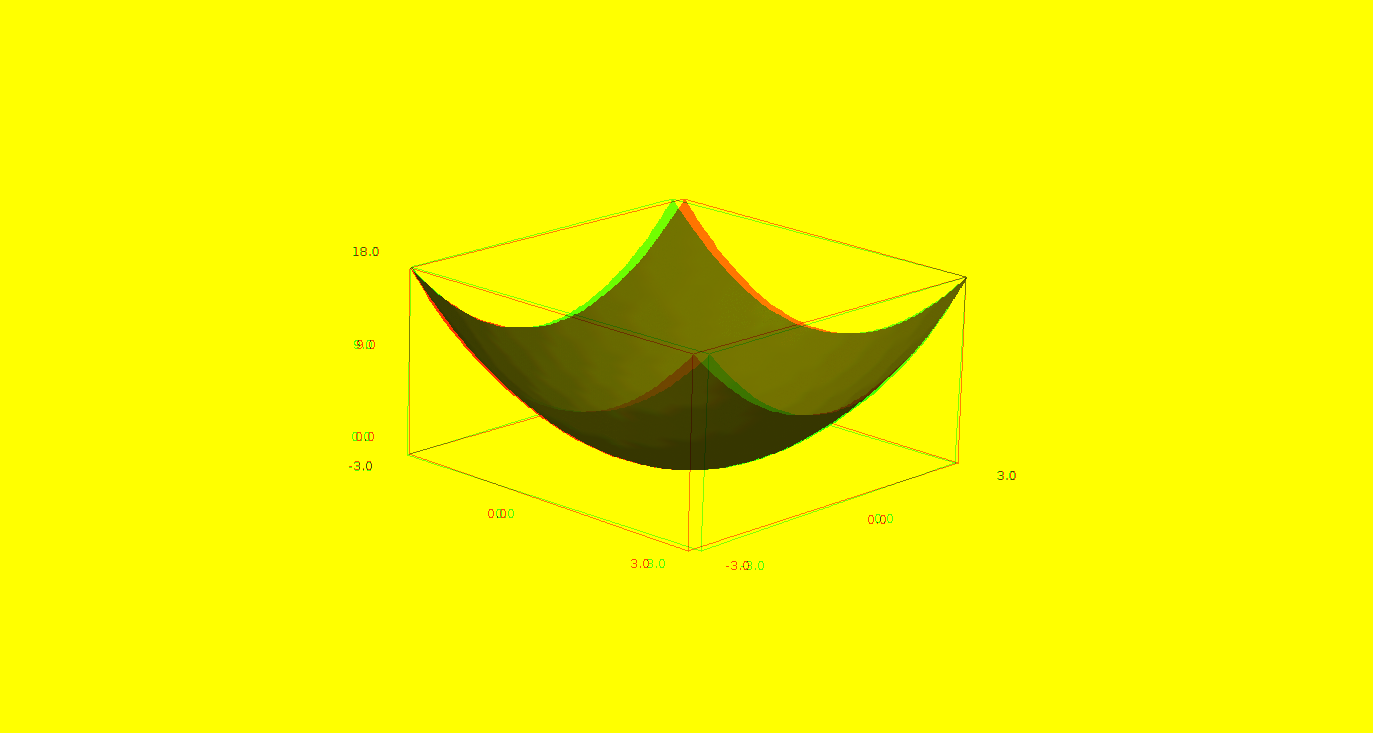
\includegraphics[width=15cm]{coupe.png}
        \else
            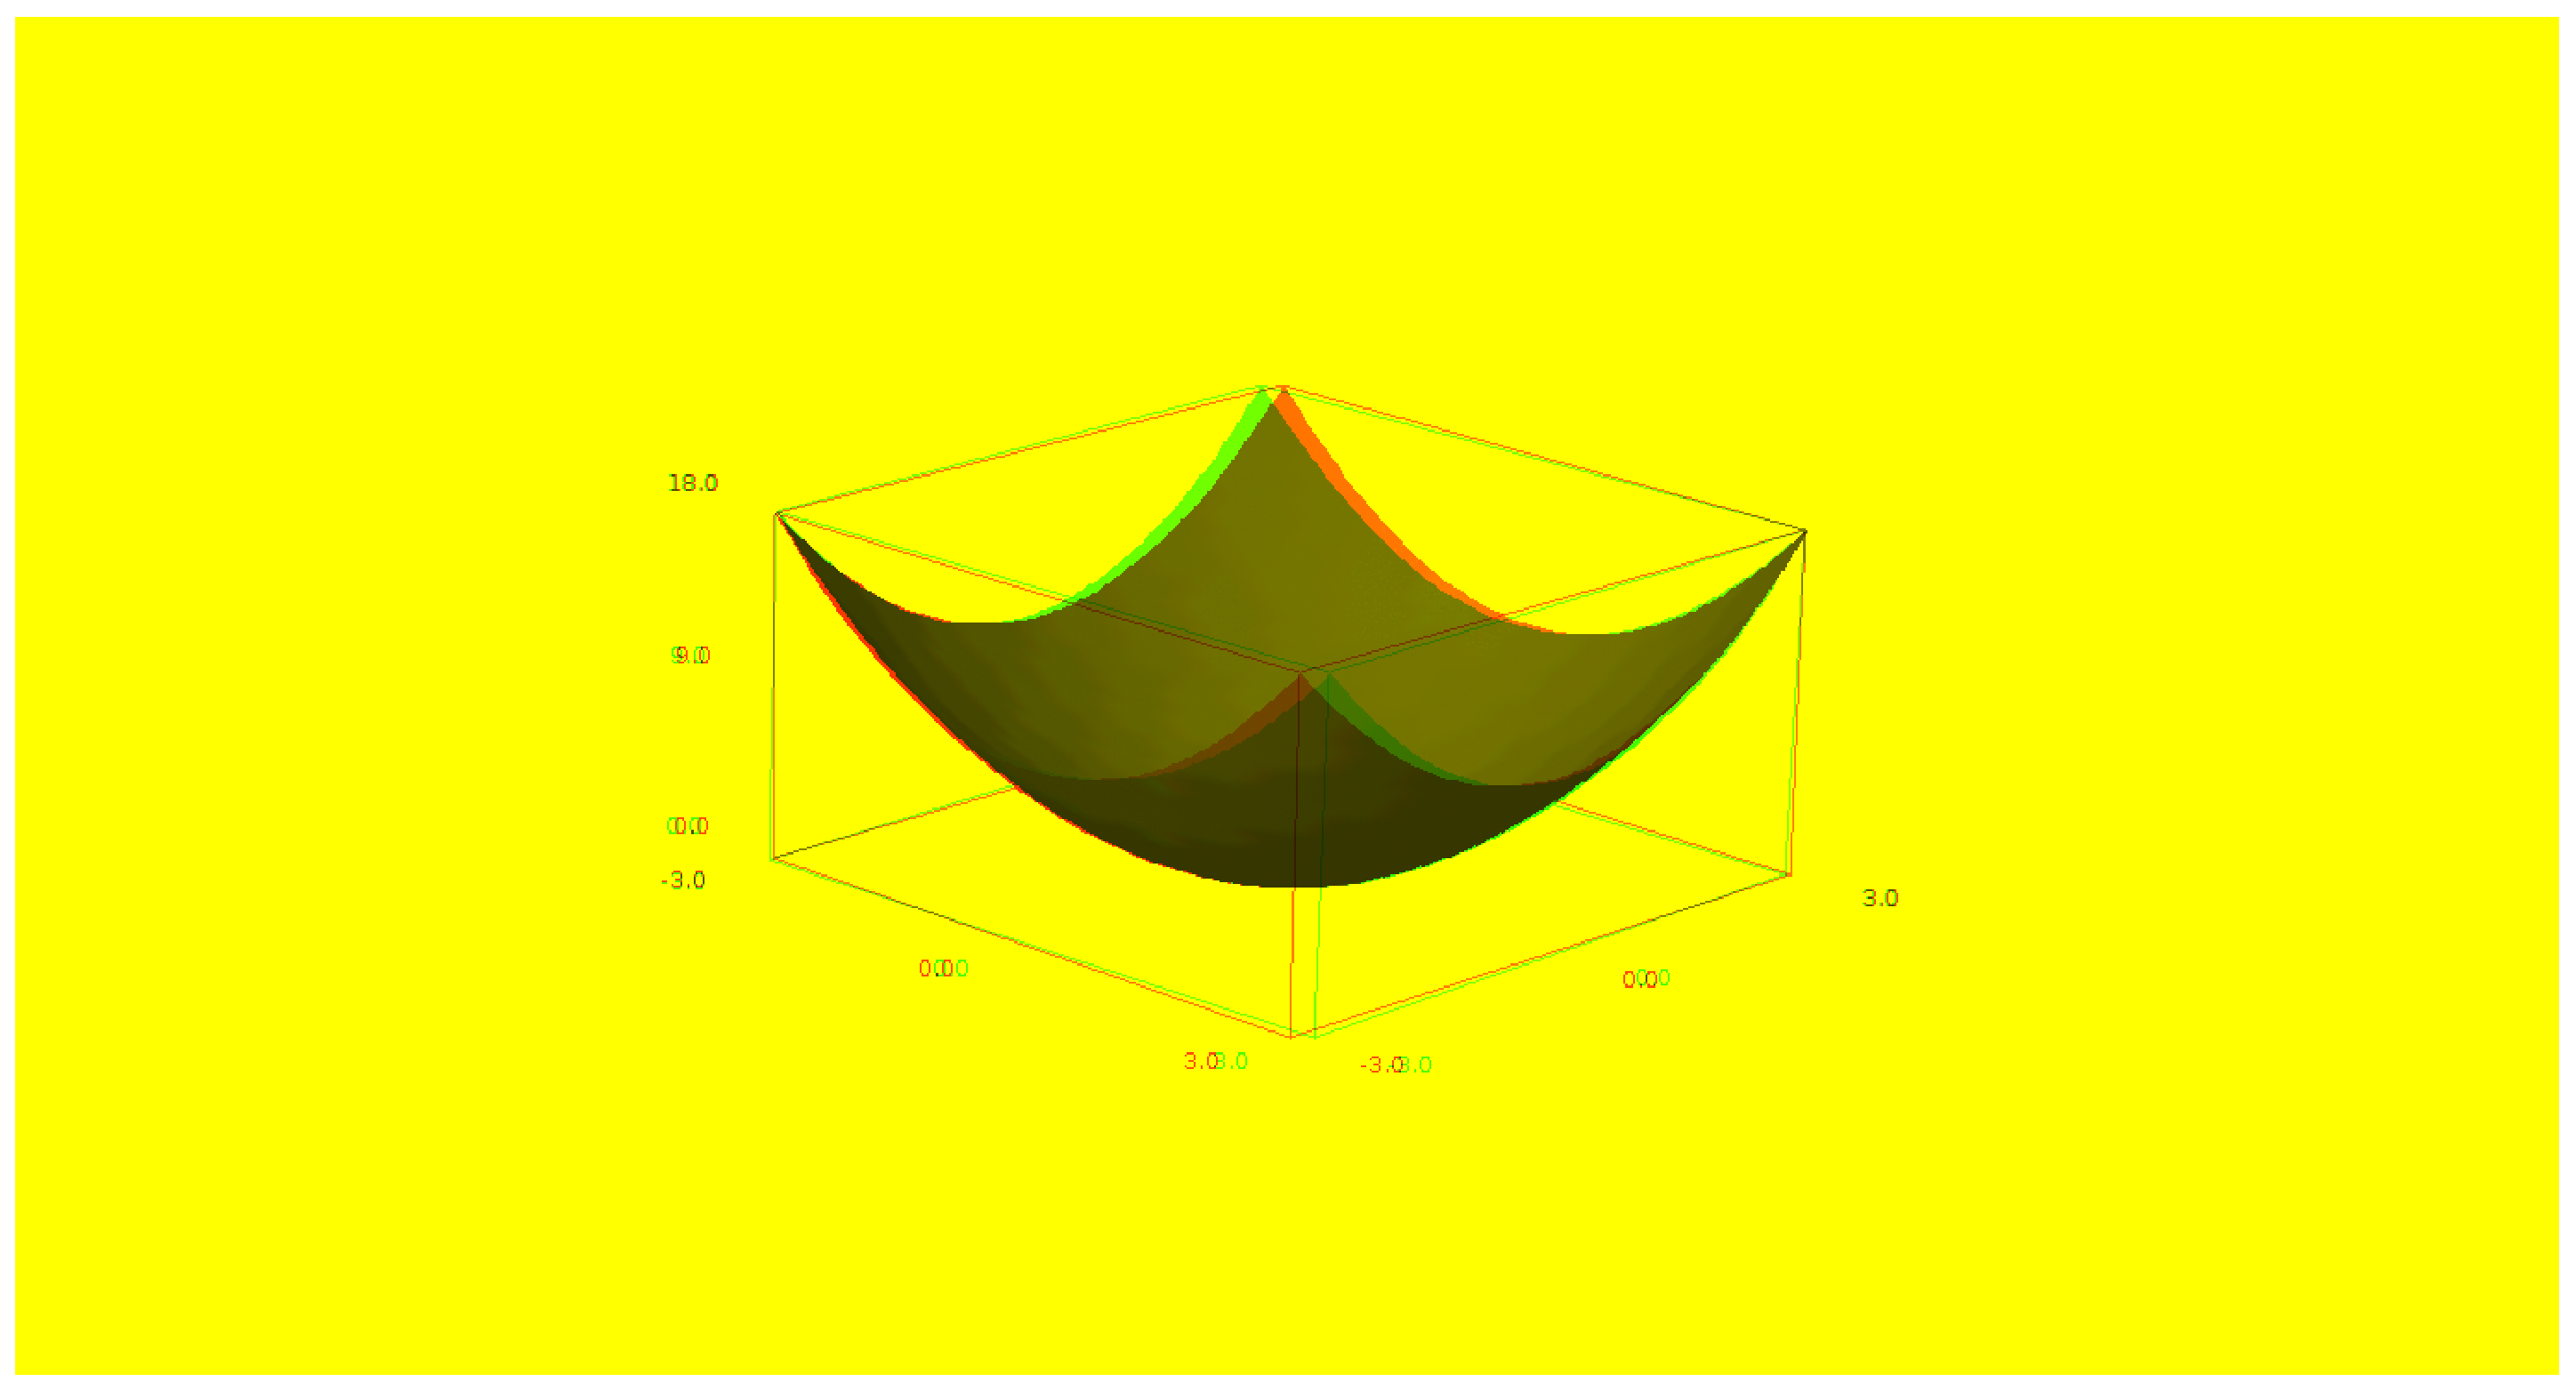
\includegraphics[width=15cm]{coupe.eps}
        \fi
    \end{center}
    À part que l'ordinateur l'a dit, est-ce qu'on peut comprendre pourquoi le graphe de la fonction $x^2+y^2$ ressemble à un bol ? En coordonnées cylindriques, le graphe s'écrit
    \begin{equation}
        z=r^2.
    \end{equation}
    Donc il se fait que plus on s'éloigne du point $(0,0)$ dans le plan $XY$, plus le graphe va monter. Et il monte à quelle vitesse ? Il monte à la vitesse $r^2$. Il s'agit donc de dessiner la fonction $z=r^2$ dans le plan et de la «faire tourner».

\end{example}

%+++++++++++++++++++++++++++++++++++++++++++++++++++++++++++++++++++++++++++++++++++++++++++++++++++++++++++++++++++++++++++
\section{Courbes de niveau}
%+++++++++++++++++++++++++++++++++++++++++++++++++++++++++++++++++++++++++++++++++++++++++++++++++++++++++++++++++++++++++++

Une technique utile pour se faire une idée de la forme d'une fonction en trois dimensions est de tracer les \defe{courbes de niveau}{courbe de niveau}. La courbe de niveau de hauteur $h$ est la courbe dans le plan donnée par l'équation
\begin{equation}
    f(x,y)=h.
\end{equation}

\begin{example}

    Dessinons par exemple les courbes de niveau de la fonction
    \begin{equation}
        f(x,y)=x+y+2.
    \end{equation}
    La courbe de niveau $h$ est donnée par l'équation $x+y+2=h$, c'est à dire
    \begin{equation}
        y(x)=-x+h-2.
    \end{equation}
    Par conséquent la courbe de niveau de hauteur $0$ est $y=-x-2$, celle de hauteur $5$ est $y=-x+3$, etc.
    
    Nous pouvons également nous aider de Sage pour ce faire :
    \begin{verbatim}
----------------------------------------------------------------------
| Sage Version 4.6.1, Release Date: 2011-01-11                       |
| Type notebook() for the GUI, and license() for information.        |
----------------------------------------------------------------------
sage: f(x,y)=x+y+2
sage: var('h')                   
h
sage: niveau(h,x)=solve(f(x,y)==h,y)[0].rhs()
sage: g1(x)=niveau(1,x)
sage: g1
x |--> -x - 1
    \end{verbatim}
    Ici la fonction \verb+g1+ est la courbe de niveau $1$. 

    Si on veut faire tracer une courbe de niveau, Sage peut le faire :
    \begin{verbatim}
        sage: implicit_plot(f(x,y)==1,(x,-3,3),(y,-4,4))
    \end{verbatim}
    Cela tracera la courbe de niveau $h=1$ dans la partie du plan $x\in\mathopen[ -3 , 3 \mathclose]$ et $y\in\mathopen[ -4,4 ,  \mathclose]$.
    
\end{example}

Il est bien entendu possible de créer automatiquement $50$ courbes de niveau et de demander de les tracer toutes sur le même graphe.
\VerbatimInput[tabsize=3]{courbeNiveau.py}

Le résultat est :

\begin{center}
    \ifpdf
        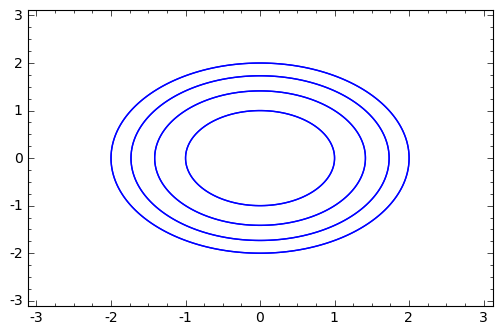
\includegraphics[width=8cm]{niveauCercles.png}
    \else
        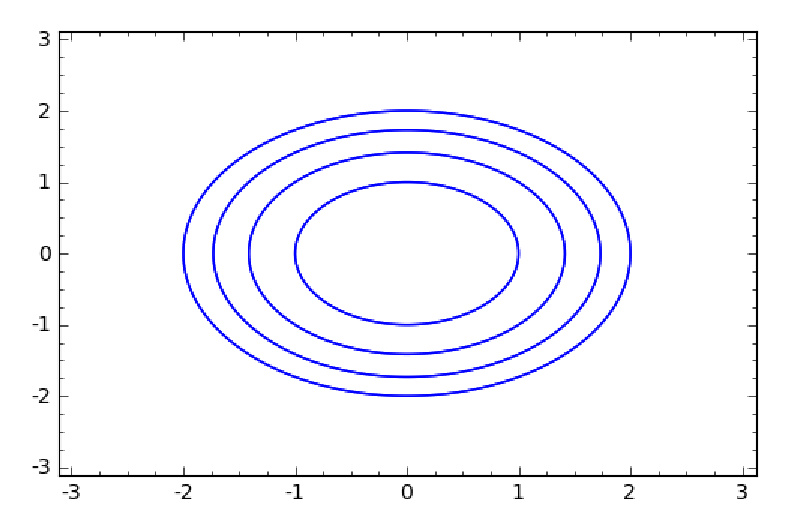
\includegraphics[width=8cm]{niveauCercles.eps}
    \fi
\end{center}
Notez que les courbes sont censées être des cercles : les axes $X$ et $Y$ n'ont pas la même échèle. Vous trouverez sur \href{http://uw.sagenb.org/home/pub/23/}{cette page} tout ce qu'il vous faudra pour créer des courbes de niveau avec Sage.

\begin{example}
    Un exemple plus riche en enseignements est celui de la fonction
    \begin{equation}
        f(x,y)=x^2-y^2.
    \end{equation}
    La courbe de niveau $h$ est donnée par l'équation $x^2-y^2=h$.

    Commençons par $h=0$. Dans ce cas nous avons $(x+y)(x-y)=0$ et par conséquent les courbes de niveau de hauteur zéro sont les deux droites $x+y=0$ et $x-y=0$.

    Voyons ensuite la courbe de niveau $h=1$. Cela est l'équation $x^2-y^2=1$, c'est à dire
    \begin{equation}
        y(x)=\pm\sqrt{x^2-1}.
    \end{equation}
    C'est une fonction qui n'est définie que pour $| x |\geq 1$. Avec $x=1$ nous avons $y=1$. Ensuite, lorsque $x$ grandit, $y$ grandit également, mais la courbe ne peut pas croiser la courbe de niveau $h=0$. Donc, suivant les notations de la figure \ref{LabelFigNiveauHyperbole}, la courbe de niveau «part» de $P$ et doit monter sans croiser les diagonales.

    \newcommand{\CaptionFigNiveauHyperbole}{La courbe de niveau $h=1$ de $x^2-y^2$. Notez qu'elle est en deux morceaux.}
    \input{Fig_NiveauHyperbole.pstricks}

    En ce qui concerne la courbe de niveau $h=-1$, elle correspond à la courbe $y=\pm\sqrt{1+x^2}$ qui est définie pour tous les $x\in\eR$. Le même raisonnement que précédemment nous amène à la figure \ref{LabelFigNiveauHyperboleDeux}.
\newcommand{\CaptionFigNiveauHyperboleDeux}{La courbe de niveau $x^2-y^2=-1$.}
\input{Fig_NiveauHyperboleDeux.pstricks}


\end{example}

Une autre façon de voir les courbe de niveau est de dire que la courbe de niveau de hauteur $h$ est la projection dans le plan $XY$ de la section du graphe de $f$ par le plan $z=h$.

On peut également définir le graphe de fonctions de trois (ou plus) variables. Le graphe de la fonction $f\colon D\subset\eR^3\to \eR$ est l'ensemble
\begin{equation}
    \big\{ \big( x,y,z,f(x,y,z) \big)\tq (x,y,z)\in D \big\}\subset \eR^4.
\end{equation}
De tels graphes ne peuvent pas être représentés sur une feuille de papier. Il est toutefois possible de définir les ensembles de niveaux :
\begin{equation}
    E_h=\big\{ (x,y,z)\in D\tq  f(x,y,z)=h\big\}.
\end{equation}
Ce sont des surfaces dans $\eR^3$ que l'on peut dessiner.

\begin{example}
    Les surfaces de niveau de la fonction $f(x,y,z)=x^2+y^2+z^2$ sont des sphères. Il n'y a pas de surfaces de niveau pour les «hauteurs» négatives.
\end{example}

\begin{example}
    Considérons la fonction $f(x,y,z)=x^2+y^2-z^2$. En coordonnées cylindrique, cette fonction s'écrit
    \begin{equation}
        f(r,\theta,z)=r^2-z^2.
    \end{equation}
    La surface de niveau $0$ est donnée par l'équation $r=| z |$. Cela fait un cercle à chaque hauteur, dont le rayon grandit linéairement avec la hauteur; le tout est donc un cône. C'est d'ailleurs le cône obtenu par rotation de la courbe de niveau $h=0$ que nous avions obtenue pour la fonction $x^2-y^2$.

    En ce qui concerne les ensembles de niveau positifs, ils sont donnés par
    \begin{equation}
        z=\pm\sqrt{x^2+y^2-h}.
    \end{equation}
    Notez qu'ils ne sont pas définis pour $r\geq h$. Cela pose un petit problème quand on veut le tracer à l'ordinateur :
    \begin{verbatim}
----------------------------------------------------------------------
| Sage Version 4.6.1, Release Date: 2011-01-11                       |
| Type notebook() for the GUI, and license() for information.        |
----------------------------------------------------------------------
sage: var('x,y')
(x, y)
sage: f(x,y)=sqrt(x**2+y**2-3)
sage: F=plot3d(f(x,y),(x,-5,5),(y,-5,5)) 
sage: G=plot3d(-f(x,y),(x,-5,5),(y,-5,5))    
sage: F+G
    \end{verbatim}
Le résultat est\footnote{Encore une fois : ça donne mieux à l'écran, et vous pouvez le faire bouger; je vous encourage à le faire !} :
    \begin{center}
        \ifpdf
            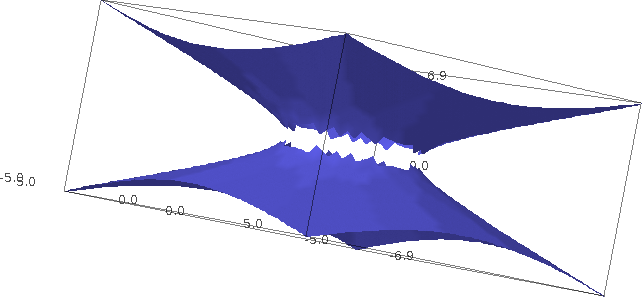
\includegraphics[width=15cm]{AdSmauvais.png}
        \else
            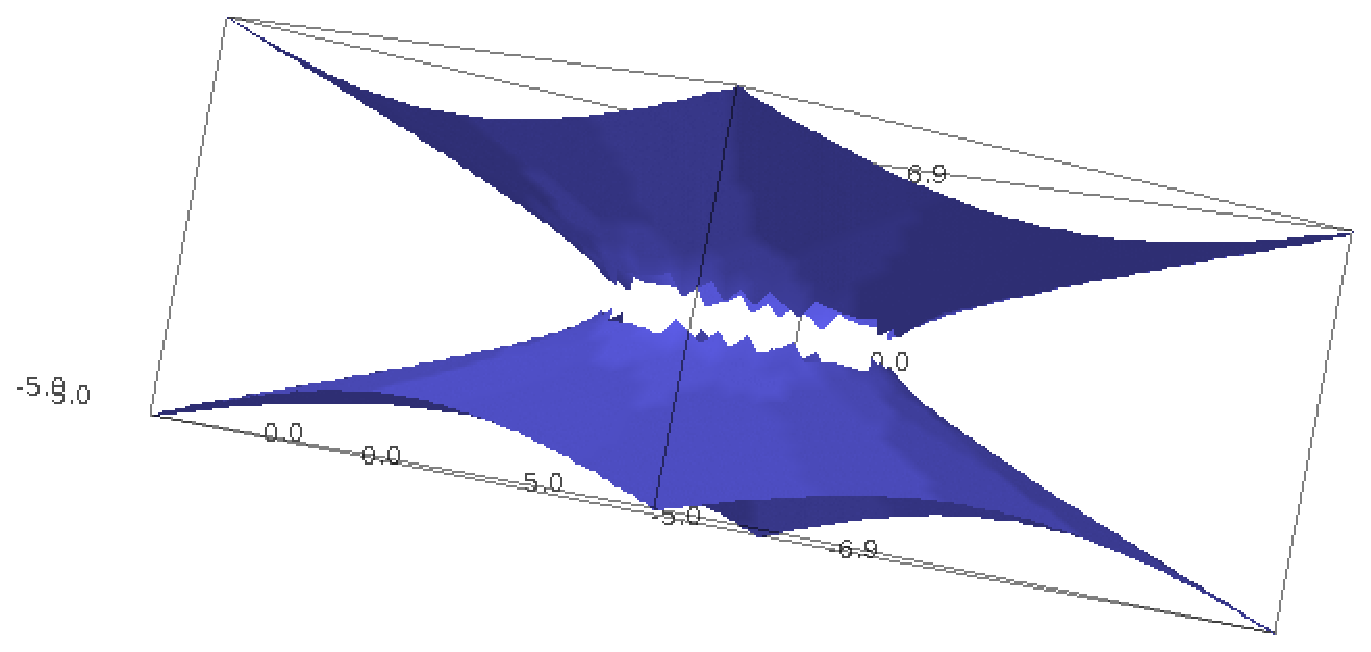
\includegraphics[width=15cm]{AdSmauvais.eps}
        \fi
    \end{center}
    On voit qu'il y a un grand trou au centre correspondant aux $z$ proches de zéro. Or d'après l'équation, il n'en est rien : en $z=0$ il y a bel et bien tout un cercle. Afin d'obtenir une meilleur image, il faut demander de tracer avec un maillage plus fin :
    \begin{verbatim}
----------------------------------------------------------------------
| Sage Version 4.6.1, Release Date: 2011-01-11                       |
| Type notebook() for the GUI, and license() for information.        |
----------------------------------------------------------------------
sage: var('x,y')
(x, y)
sage: f(x,y)=sqrt(x**2+y**2-3)
sage: F=plot3d(f(x,y),(x,-5,5),(y,-5,5),plot_points=300) 
sage: G=plot3d(-f(x,y),(x,-5,5),(y,-5,5),plot_points=300)
sage: F+G
    \end{verbatim}
    Le temps de calcul est un peu plus long, mais le résultat est meilleur :
    \begin{center}
        \ifpdf
            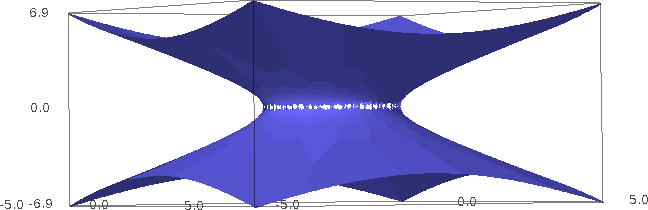
\includegraphics[width=15cm]{AdSbon.png}
        \else
            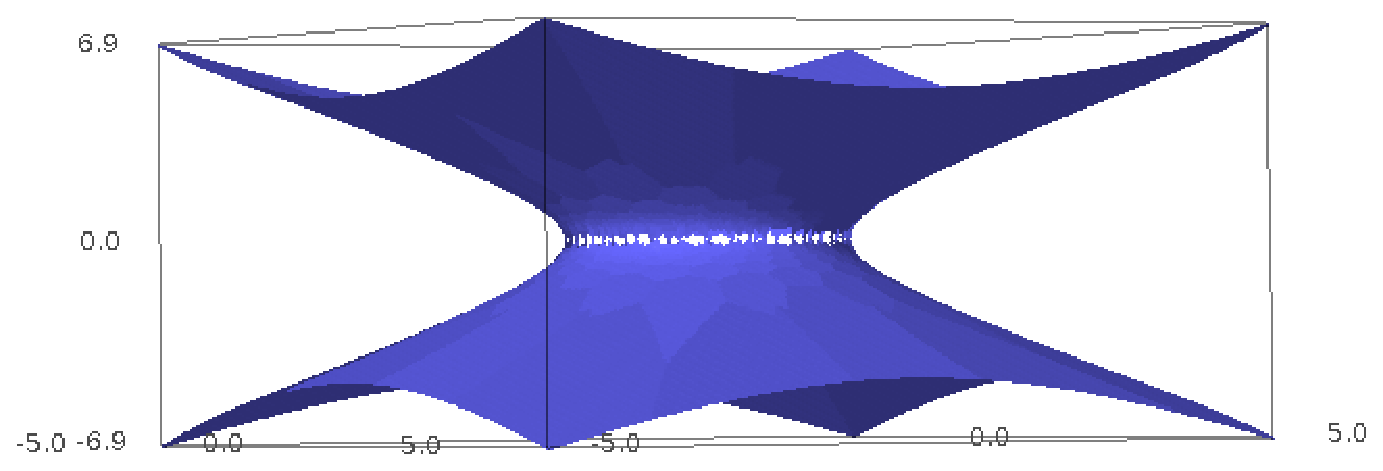
\includegraphics[width=15cm]{AdSbon.eps}
        \fi
    \end{center}
\end{example}

%+++++++++++++++++++++++++++++++++++++++++++++++++++++++++++++++++++++++++++++++++++++++++++++++++++++++++++++++++++++++++++
\section{Dérivées partielles}
%+++++++++++++++++++++++++++++++++++++++++++++++++++++++++++++++++++++++++++++++++++++++++++++++++++++++++++++++++++++++++++

Soit $f\colon \eR^2\to \eR$ une fonction de deux variables et soit $(a,b)\in\eR^2$. La façon la plus naturelle de définir une dérivée à deux variables est de considérer les \defe{dérivées partielles}{dérivée!partielle} définies par
\begin{equation}
    \begin{aligned}[]
        \frac{ \partial f }{ \partial x }(a,b)&=\lim_{x\to a} \frac{ f(x,b)-f(a,b) }{ x-a }\\
        \frac{ \partial f }{ \partial y }(a,b)&=\lim_{y\to b} \frac{ f(a,y)-f(a,b) }{y-b}.
    \end{aligned}
\end{equation}
Ces nombres représentent la façon dont le nombre $f(x,y)$ varie lorsque soit seul $x$ varie soit seul $y$ varie. Les dérivées partielles se calculent de la même façon que les dérivées normales. Pour calculer $\partial_xf$, on fait «comme si» $y$ était une constante, et pour calculer $\partial_yf$, on fait comme si $x$ était une constante.

\begin{example}
    Considérons $f(x,y)=x^2y+y^2 e^{x}$. Les dérivées partielles sont
    \begin{equation}
        \begin{aligned}[]
            \frac{ \partial f }{ \partial x }&=2xy+y^2e^x\\
            \frac{ \partial f }{ \partial y }&=x^2+2ye^x.
        \end{aligned}
    \end{equation}
\end{example}

Cet exemple était l'exemple facile où tout se passe bien.

\begin{example}
    Les choses sont moins simples lorsqu'on considère la fonction suivante :
    \begin{equation}
        f(x,y)=\begin{cases}
            \frac{ xy }{ x^2+y^2 }    &   \text{si $(x,y)\neq(0,0)$}\\
            0    &    \text{si $(x,y)=(0,0)$}.
        \end{cases}
    \end{equation}
    On voit que pour tout $x$ et tout $y$, nous avons $f(x,0)=f(0,y)=0$. Donc cette fonction est nulle sur les axes horizontaux et verticaux. Nous avons en particulier
    \begin{equation}
        \begin{aligned}[]
            \frac{ \partial f }{ \partial x }(0,0)&=0\\
            \frac{ \partial f }{ \partial y }(0,0)&=0.
        \end{aligned}
    \end{equation}
    Donc ces dérivées partielles existe.

    Il n'est par contre pas question de dire que cette fonction «va bien» autour du point $(0,0)$. En effet si nous regardons sa valeur sur la droite diagonale $y=x$, nous avons
    \begin{equation}
        f(x,x)=\frac{ x^2 }{ 2x^2 }=\frac{ 1 }{2}.
    \end{equation}
    Par conséquent si nous suivons la fonction le long de la droite $y=x$, la hauteur vaut $\frac{ 1 }{2}$ en permanence, saut juste en $(0,0)$ où la fonction fait un grand plongeon !
    \begin{verbatim}
    sage: var('x,y')
    (x, y)
    sage: f(x,y)=(x*y)/(x**2+y**2)
    sage: plot3d(f,(x,-2,2),y(-2,2))
    \end{verbatim}

    D'ailleurs elle fait un plongeon le long de toutes les droites (sauf verticale et horizontale). En effet si nous regardons la fonction le long de la droite $y=mx$, nous avons
    \begin{equation}
        f(x,mx)=\frac{ mx^2 }{ x^2+m^2x^2 }=\frac{ m }{ 1+m^2 }.
    \end{equation}
    La fonction est donc \emph{constante} sur chacune de ces droites. Il n'est donc pas question de dire que cette fonction est «dérivable» en $(0,0)$, vu qu'elle fait des grands sauts dans presque toutes les directions.
\end{example}

Nous devons donc trouver mieux que les dérivées partielles pour étudier le comportement des fonctions un peu problématiques.

Nous nous souvenons de l'équation \eqref{EqCodeDerviffxam} qui nous dis que pour une fonction d'une variable la dérivabilité signifiait qu'il existait un nombre $\ell$ et une fonction $\alpha$ tels
\begin{equation}
    f(x)=f(a)+\ell(x-a)+(x-a)\alpha(x-a)
\end{equation}
et $\lim_{t\to 0} \alpha(t)=0$. 

En nous inspirant de cela, nous posons la définition suivante.
\begin{definition}      \label{DefDiffabel}
    Une fonction $f\colon \eR^2\to \eR$ est \defe{différentiable}{différentiable} au point $(a,b)\in\eR^2$ si il existe deux nombres $\ell_1$, $\ell_2$ ainsi qu'une fonction $\alpha$ tels que
    \begin{equation}\label{EqCondDiffabel}
        \begin{aligned}[]
            f(x,y)=f(a,b)&+\ell_1(x-a)+\ell_2(y-b)\\
                    &+\sqrt{(x-a)^2+(y-b)^2}\alpha\big( \sqrt{(x-a)^2+(y-b)^2} \big).
        \end{aligned}
    \end{equation}
\end{definition}

En utilisant la notation vectorielle, cela peut être écrite sous forme très compacte. Posons
\begin{equation}
    \begin{aligned}[]
        \ell&=\begin{pmatrix}
            \ell_1    \\ 
            \ell_2    
        \end{pmatrix},&
        X&=\begin{pmatrix}
            x    \\ 
            y    
        \end{pmatrix},&
        P&=\begin{pmatrix}
            a    \\ 
            b    
        \end{pmatrix}.
    \end{aligned}
\end{equation}
Alors la condition \eqref{EqCondDiffabel} s'écrit
\begin{equation}
    f(X)=f(P)+\ell\cdot(X-P)+\| X-P \|\alpha\big( \| X-P \| \big).
\end{equation}

\begin{proposition}
    Si $f$ est différentiable en $(a,b)$, alors les nombres $\partial_xf(a,b)$ et $\partial_yf(a,b)$ existent et valent respectivement $\ell_1$ et $\ell_2$.
\end{proposition}

\begin{proof}
    Afin de calculer la dérivée partielle dans la direction de $x$, nous posons $y=b$ dans la condition \eqref{EqCondDiffabel} :
    \begin{equation}
        f(x,b)=f(a,b)+\ell_1(x-a)+| x-a |\alpha\big( | x-a | \big),
    \end{equation}
    et donc
    \begin{equation}
        \frac{ f(x,b)-f(a,b) }{ x-a }=\ell_1\pm\alpha\big( | x-a | \big).
    \end{equation}
    Ici le $\pm$ est parce que nous avons divisé $(x-a)$ par $| x-a |$. Quel que soit ce signe, de toutes façons la limite du membre de droite lorsque $x$ tend vers $a$ est $\ell_1$ parce que $\lim_{x\to a} \alpha(| x-a |)=0$.

    Afin de prouver l'existence de la dérivée dans la direction de $y$, nous procédons de la même manière, mais en partant de $f(a,y)$.
\end{proof}

\begin{proposition}
    Si $f$ est différentiable au point $(a,b)$, alors elle y est continue, c'est à dire que
    \begin{equation}
        \lim_{(x,y)\to(a,b)}f(x,y)=f(a,b).
    \end{equation}
\end{proposition}

\begin{proof}
    Si nous considérons la différence entre $f(x,y)$ et $f(a,b)$, nous avons (en notations matricielle) :
    \begin{equation}
        | f(X)-f(P) |=| \ell\cdot(X-P)+\| X-P \|\alpha(\| X-P \|) |.
    \end{equation}
    Le membre de droite tend évidemment vers zéro lorsque $X$ tend vers $P$.
\end{proof}
    \begin{remark}
        Attention : ceci n'est pas une preuve. En effet, dans la mesure où nous n'avons même pas donné de définition de la limite, il n'est pas possible de donner une \emph{vraie} preuve de quoi que ce soit. 
    \end{remark}

Nous avons vu que l'existence des deux dérivées partielles ne permettait pas de conclure à la différentiabilité. La différentiabilité d'une fonction peut néanmoins être déduites d'une étude plus précise des dérivées partielles. Nous avons pour cela les propositions \ref{PropExistDiffUn} et \ref{PropExistDiffDeux}

\begin{proposition} \label{PropExistDiffUn}
    Soit $f$ une fonction de $x$ et $y$ et un point $(a,b)\in\eR^2$. Si les nombres $\partial_xf(a,b)$ et $\partial_yf(a,b)$ existent et si il existe une fonction $\alpha\colon \eR\to \eR$ telle que
    \begin{equation}        \label{eqCritDifffabsrt}
        \begin{aligned}[]
            f(x,y)=f(a,b)&+\frac{ \partial f }{ \partial x }(a,b)(x-a)+\frac{ \partial f }{ \partial y }(a,b)(y-b)\\
            &+\| (x,y)-(a,b) \| \alpha\Big( \| (x,y)-(a,b) \| \Big)
        \end{aligned}
    \end{equation}
    et
    \begin{equation}
        \lim_{t\to 0} \alpha(t)=0,
    \end{equation}
    alors $f$ est différentiable en $(a,b)$.
\end{proposition}
Dans cet énoncé nous avons écrit $d\big( (x,y),(a,b) \big)$ la distance entre $(x,y)$ et $(a,b)$, c'est à dire le nombre $\sqrt{(x-a)^2+(y-b)^2}$. Afin d'écrire l'équation \eqref{eqCritDifffabsrt} sous forme plus compacte, nous introduisons le vecteur
\begin{equation}
    \nabla f(a,b)=\begin{pmatrix}
        \frac{ \partial f }{ \partial x }(a,b)    \\ 
        \frac{ \partial f }{ \partial y }(a,b).    
    \end{pmatrix}
\end{equation}
L'équation \eqref{eqCritDifffabsrt} devient alors
\begin{equation}        \label{EqdiffComp}
    f(X)=f(P)+\nabla f(a,b)\cdot (X-P)+\| X-P \|\alpha\big( \| X-P \| \big).
\end{equation}
Le vecteur $\nabla f(a,b)$ est appelé le \defe{gradient}{gradient} de $f$ au point $(a,b)$.


\begin{proposition} \label{PropExistDiffDeux}
    Soit $f$ une fonction de deux variables admettant des dérivées partielles $\partial_xf(x,y)$ et $\partial_yf(x,y)$ qui sont elles-mêmes des fonctions continues de $x$ et $y$. Alors la fonction $f$ est différentiable partout.
\end{proposition}

\begin{remark}
    Tout ce qui a été dit, et tout ce qui sera dit, sur les fonctions a deux variables se généralise immédiatement aux fonctions à plus de variables. C'est dans ce but que la notation «compacte» utilisant les vecteurs est très pratique.
\end{remark}

Si nous remplaçons les accroissements $x-a$ et $y-b$ par $h$ et $k$, le critère de différentiabilité s'écrit
\begin{equation}
    \begin{aligned}[]
        f(a+h,b+k)=f(a,b)+\frac{ \partial f }{ \partial x }(a,b)h&+\frac{ \partial f }{ \partial y }(a,b)k\\
        &+\sqrt{h^2+k^2}\alpha\big( \sqrt{h^2+k^2} \big).
    \end{aligned}
\end{equation}
Le dernier terme du membre de droite tend vers zéro à une vitesse double lorsque $h$ et $k$ tendent vers zéro : d'une part parce que $\sqrt{h^2+k^2}$ tend vers zéro et d'autre part parce que $\alpha\big( \sqrt{h^2+k^2} \big)$ tend vers zéro. Nous avons donc la «bonne» approximation
\begin{equation}        \label{EqFormApproxfxyab}
    f(x,y)\simeq f(a,b)+\frac{ \partial f }{ \partial x }(a,b)(x-a)+\frac{ \partial f }{ \partial y }(a,b)(y-b).
\end{equation}
lorsque $(x,y)$ n'est pas trop loin de $(a,b)$. Cette expression est évidemment une généralisation immédiate de l'équation \eqref{EqfxdxSimeqfxfpx}. Elle exprime que l'on peut obtenir des information sur la valeur d'une fonction en $(x,y)$ si on peut calculer la fonction et ses dérivées en un point $(a,b)$ non loin de $(x,y)$.

Cette formule peut aussi être vue sous la forme suivante, plus pratique dans certains calculs :
\begin{equation}        \label{EqFormApproxfxyabDF}
    f(a+\Delta x,b+\Delta y)\simeq f(a,b)+\Delta x\frac{ \partial f }{ \partial x }(a,b)+\Delta y\frac{ \partial f }{ \partial y }(a,b).
\end{equation}

\begin{example}
    Prenons la fonction $f(x,y)=\cos(x)\sin(y)$ et calculons une approximation de
    \begin{equation}
        f\big( \frac{ \pi }{ 3 }+0.01,\frac{ \pi }{ 2 }+0.03 \big).
    \end{equation}
    D'abord les dérivées partielles sont
    \begin{equation}
        \begin{aligned}[]
            \frac{ \partial f }{ \partial x }(x,y)=-\sin(x)\sin(y)\\
            \frac{ \partial f }{ \partial y }(x,y)=\cos(x)\cos(y).
        \end{aligned}
    \end{equation}
    Nous allons utiliser l'approximation
    \begin{equation}
        f\big( \frac{ \pi }{ 3 }+0.01,\frac{ \pi }{ 2 }+0.03 \big)\simeq f\big( \frac{ \pi }{ 3 },\frac{ \pi }{2} \big)+0.01\frac{ \partial f }{ \partial x }\big( \frac{ \pi }{ 3 },\frac{ \pi }{2} \big)+0.03\frac{ \partial f }{ \partial y }\big( \frac{ \pi }{ 3 },\frac{ \pi }{2} \big).
    \end{equation}
    Nous avons
    \begin{equation}
        \begin{aligned}[]
            \frac{ \partial f }{ \partial x }\big( \frac{ \pi }{ 3 },\frac{ \pi }{2} \big)&=-\sin\frac{ \pi }{ 3 }\sin\frac{ \pi }{ 2 }=-\frac{ \sqrt{3} }{2}\\
            \frac{ \partial f }{ \partial y }\big( \frac{ \pi }{ 3 },\frac{ \pi }{2} \big)&=\cos\frac{ \pi }{ 3 }\cos\frac{ \pi }{ 2 }=0.
        \end{aligned}
    \end{equation}
    Par conséquent
    \begin{equation}
        f\big( \frac{ \pi }{ 3 }+0.01,\frac{ \pi }{ 2 }+0.03 \big)\simeq \frac{ 1 }{2}-0.01\frac{ \sqrt{3} }{2}=\frac{ 1 }{2}-\frac{ \sqrt{3} }{ 200 }. 
    \end{equation}
    
    \begin{verbatim}
sage: var('x,y')
(x, y)
sage: f(x,y)=cos(x)*sin(y)
sage: a=f(pi/3+0.01,pi/2+0.03)
sage: numerical_approx(a)
0.491093815387986
sage: b=1/2-sqrt(3)/200
sage: numerical_approx(b)
0.491339745962156
sage: numerical_approx(a-b)
-0.000245930574169814
    \end{verbatim}
    Cela fait une erreur de l'ordre du dix millième. 
    
\end{example}

\begin{remark}
    Les esprits les plus critiques diront que cette vérification pas Sage n'en est pas une parce que Sage a certainement utilisé un algorithme d'approximation qui se base sur la même idée que ce que nous venons de faire, et que par conséquent le fait qu'il obtienne le même résultat que nous est un peu tautologique. 
    
    Ils n'auront pas tord. Cependant, le code source de Sage est disponible publiquement\footnote{Voir \url{http://www.sagemath.org}}; vous pouvez aller le lire et vérifier qu'il y a effectivement une \emph{preuve} que le résultat fourni par Sage possède une bonne dizaine de décimales correctes. 
    
    Cette disponibilité publique du code source est une des nombreuses différence fondamentale entre Sage et votre calculatrice\footnote{et les autres logiciels de type fenêtre, pomme ou feuille d'érable.}. Dois-je vous rappeler qu'un des principes fondamentaux de l'éthique scientifique est que les résultats et les méthodes utilisées doivent être absolument ouverts à la vérification et à la critique de tous ?
\end{remark}

%---------------------------------------------------------------------------------------------------------------------------
\subsection{Différentielle}
%---------------------------------------------------------------------------------------------------------------------------

\begin{definition}      \label{DefDiffrdrr}
    Lorsque $f$ est différentiable au point $(a,b)$, on appelle \defe{différentielle}{différentielle} de $f$ l'application linéaire
    \begin{equation}        \label{EqDefDiffmapdf}
        \begin{aligned}
            df_{(a,b)}\colon \eR^2&\to \eR \\
            \begin{pmatrix}
                u_1    \\ 
                u_2    
            \end{pmatrix}&\mapsto \frac{ \partial f }{ \partial x }(a,b)u_1+\frac{ \partial f }{ \partial y }(a,b)u_2. 
        \end{aligned}
    \end{equation}
    En notations compacte :
    \begin{equation}        \label{EqdfUPnable}
        df_{P}(U)=\nabla f(P)\cdot U.
    \end{equation}
\end{definition}

Note : dans la suite nous allons rendre notre «notation compacte» plus agréable à lire en abandonnant les majuscules. L'équation \eqref{EqdfUPnable} s'écrira donc
\begin{equation}        \label{Eqdfpunfpdu}
    df_p(u)=\nabla f(p)\cdot u.
\end{equation}


%+++++++++++++++++++++++++++++++++++++++++++++++++++++++++++++++++++++++++++++++++++++++++++++++++++++++++++++++++++++++++++
\section{Plan tangent au graphe d'une fonction}
%+++++++++++++++++++++++++++++++++++++++++++++++++++++++++++++++++++++++++++++++++++++++++++++++++++++++++++++++++++++++++++

Nous avons vu que, de la même façon qu'en deux dimensions nous avions l'approximation \eqref{Eqfxsimesfa} d'une fonction par sa tangente, en trois dimensions nous avons l'approximation suivante d'une fonction de deux variables :
\begin{equation}
    f(x,y)\simeq f(a,b)+\frac{ \partial f }{ \partial x }(a,b)(x-a)+\frac{ \partial f }{ \partial y }(a,b)(y-b)
\end{equation}
lorsque $(x,y)$ n'est pas trop loin de $(a,b)$. Cela signifie que le graphe de $f$ ressemble au graphe de la fonction $T_{(a,b)}$ donnée par
\begin{equation}
    T_{(a,b)}(x,y)=f(a,b)+\frac{ \partial f }{ \partial x }(a,b)(x-a)+\frac{ \partial f }{ \partial y }(a,b)(x-a).
\end{equation}
En notations compactes :
\begin{equation}
    T_p(x)=f(p)+\nabla f(p)\cdot (x-p).
\end{equation}
Le graphe de la fonction $T_p$ sera le \defe{plan tangent}{plan tangent} au graphe de $f$ au point $p$. L'équation du plan tangent sera donc
\begin{equation}
    z-f(p)=\nabla f(p)\cdot (x-p).
\end{equation}

\begin{remark}
    Lorsque nous utilisons la notation vectorielle, la lettre «$x$» désigne le vecteur $(x,y)$. Il faut être attentif. Dans un cas $x$ est un vecteur dans l'autre c'est une composante d'un vecteur.
\end{remark}




%+++++++++++++++++++++++++++++++++++++++++++++++++++++++++++++++++++++++++++++++++++++++++++++++++++++++++++++++++++++++++++
\section{Dérivée directionnelle}
%+++++++++++++++++++++++++++++++++++++++++++++++++++++++++++++++++++++++++++++++++++++++++++++++++++++++++++++++++++++++++++

Nous sommes capables de dériver une fonction de deux variables $f(x,y)$ par rapport à $x$ et par rapport à $y$. C'est à dire que nous sommes capables de donner la variation de la fonction lorsqu'on bouge le long des axes horizontal et vertical. Il est évidemment souhaitable de parler de la variation de la fonction lorsqu'on se déplace le long d'autre droites.

Soit donc $u=\begin{pmatrix}
    u_1    \\ 
    u_2    
\end{pmatrix}$ un vecteur unitaire (c'est à dire $u_1^2+u_2^2=1$), et considérons la fonction de une variable
\begin{equation}
    \begin{aligned}
        \varphi\colon \eR&\to \eR \\
        t&\mapsto f(a+tu_1,b+tu_2). 
    \end{aligned}
\end{equation}
La fonction $\varphi$ n'est rien d'autre que la fonction $f$ vue le long de la droite de direction donnée par le vecteur $u$. Nous pouvons aussi l'écrire $\varphi(t)=f(p+tu)$.

\begin{proposition}
    Si $f$ est différentiable en $(a,b)$ alors la fonction $\varphi$ est dérivable en $0$ et on a
    \begin{equation}
        \varphi'(0)=\nabla f(p)\cdot u
    \end{equation}
    où nous avons noté $p=(a,b)$.
\end{proposition}

\begin{proof}
    Récrivons la formule \eqref{EqdiffComp} sous la forme
    \begin{equation}
        f(x)=f(p)+\nabla f(p)\cdot (x-p)+\| x-p \|\alpha(\| x-p \|).
    \end{equation}
    Cela étant vrai pour tout $x$, nous l'écrivons en particulier pour $x=p+tu$ où $t$ est un réel et $u$ est le vecteur unitaire choisi. Nous avons donc
    \begin{equation}
        f(p+tu)=f(p)+t\nabla f(p)\cdot u+\| tu \|\alpha(\| tu \|).
    \end{equation}
    En utilisant le fait que $u$ est unitaire, $\| tu \|=| t |\| u \|=| t |$. La dérivée de $\varphi$ en $0$ est alors donnée par
    \begin{equation}
        \lim_{t\to 0} \frac{ f(p+tu)-f(p) }{ t }=\lim_{t\to 0} \nabla f(p)\cdot u+\alpha(| t |).    
    \end{equation}
    Lorsque nous prenons la limite, le membre de gauche devient $\varphi'(0)$ tandis que dans le membre de droite, le second terme disparaît. Nous avons finalement
    \begin{equation}
        \varphi'(0)=\nabla f(p)\cdot u
    \end{equation}
\end{proof}

\begin{definition}
    Le nombre
    \begin{equation}
        \lim_{t\to 0} \frac{ f\big( a+tu_1,b+tu_2 \big)-f(a,b) }{ t }
    \end{equation}
    est la \defe{dérivée directionnelle}{dérivée!directionnelle} de $f$ dans la direction de $u$ au point $(a,b)$. Il sera noté
    \begin{equation}
        \frac{ \partial f }{ \partial u }(a,b),
    \end{equation}
    ou plus simplement $\partial_uf(a,b)$.
\end{definition}

Lorsque $f$ est différentiable, la dérivée directionnelle est donnée par
\begin{equation}        \label{EqDerDirnablau}
    \frac{ \partial f }{ \partial u }(p)=\nabla f(p)\cdot u.
\end{equation}

En combinant avec l'équation \eqref{Eqdfpunfpdu}, nous avons la suite d'égalités
\begin{equation}        \label{Eqsuitedfnfdsdfu}
    df_p(u)=\nabla f(p)\cdot u=\frac{ \partial f }{ \partial x }(p)u_1+\frac{ \partial f }{ \partial y }(p)u_2+\frac{ \partial f }{ \partial z }(p)u_3=\frac{ \partial f }{ \partial u }(p).
\end{equation}
La dernière équation est seulement vraie si $\| u \|=1$.

%---------------------------------------------------------------------------------------------------------------------------
\subsection{Gradient : direction de plus grande pente}
%---------------------------------------------------------------------------------------------------------------------------

Étant donné que $u$ est de norme $1$, l'inégalité de Cauchy-Schwartz donne
\begin{equation}
    \big| \nabla f(a,b)\cdot \begin{pmatrix}
        u_1    \\ 
        u_2    
    \end{pmatrix}\big|\leq \| \nabla f(a,b) \|.
\end{equation}
Donc
\begin{equation}
    -\| \nabla f(p) \|\leq \nabla f(p)\cdot u\leq\| \nabla f(p) \|.
\end{equation}
La norme de la dérivée directionnelle (qui est la valeur absolue du nombre au centre) est donc «coincée» entre $-\| \nabla f(p) \|$ et $\| \nabla f(p) \|$. Prenons par exemple
\begin{equation}
    u=\frac{ \nabla f(p) }{ \| \nabla f(p) \| }.
\end{equation}
Dans ce cas, nous avons exactement
\begin{equation}
    \nabla f(p)\cdot u=\| \nabla f(p) \|,
\end{equation}
qui est la valeur maximale que la dérivée directionnelle peut prendre.

La direction du gradient est donc la direction suivant laquelle la dérivée directionnelle est la plus grande. Pour la même raison, la dérivée directionnelle est la plus petite dans le sens opposé au gradient.

En termes bien clairs : lorsqu'on veut aller le plus vite possible au ski, on prend la direction du gradient de la piste de ski. C'est dans cette direction que ça descend le plus vite. Dans quelle direction vont les débutants ? Ils vont perpendiculairement à la pente (ce qui ennuie tout le monde, mais c'est un autre problème). Les débutants vont donc dans la direction perpendiculaire au gradient. Prenons donc $u\perp \nabla f(p)$ et calculons la dérivée directionnelle de $f$ dans la direction $u$ en utilisant la formule \ref{EqDerDirnablau} :
\begin{equation}
    \frac{ \partial f }{ \partial u }(p)=\nabla f(p)\cdot u=0
\end{equation}
parce que nous avons choisit $u\perp \nabla f(p)$. Nous voyons donc que les débutants en ski ont eu la bonne intuition que la direction dans laquelle la piste ne descend pas, c'est la direction perpendiculaire au gradient.

C'est aussi pour cela que l'on a tendance à faire du zig-zag à vélo lorsqu'on monte une pente très forte et qu'on est fatigué. C'est toujours pour cela que les routes de montagne font de longs lacets. La montée est moins rude en suivant une direction proche d'être perpendiculaire au gradient !

\begin{theorem}
    Le gradient des fonction suit à peu près les mêmes règles que les dérivées. Soient $f$ et $g$ deux fonctions différentiables. Nous avons entre autres
    \begin{enumerate}
        \item
            $\nabla(f+g)=\nabla f+\nabla g$;
        \item
            $\nabla(fg)(a,b)=g(a,b)\nabla f(a,b)+f(a,b)\nabla g(a,b)$;
        \item
            Dès que $g(a,b)\neq 0$, nous avons
            \begin{equation}
                \nabla\frac{ f }{ g }=\frac{ g(a,b)\nabla f(a,b)-f(a,b)\nabla g(a,b) }{ g(a,b)^2 }.
            \end{equation}
    \end{enumerate}
\end{theorem}



\chapter{Champs de vecteurs}
% This is part of Mes notes de mathématique
% Copyright (c) 2011-2012,2015
%   Laurent Claessens
% See the file fdl-1.3.txt for copying conditions.

Les champs de vecteurs et tout ce qui s'y rapportent jouent un rôle crucial en électromagnétisme. Voir par exemple \cite{Schomblond_em}.

%+++++++++++++++++++++++++++++++++++++++++++++++++++++++++++++++++++++++++++++++++++++++++++++++++++++++++++++++++++++++++++
\section{Les fonctions à valeurs vectorielles}
%+++++++++++++++++++++++++++++++++++++++++++++++++++++++++++++++++++++++++++++++++++++++++++++++++++++++++++++++++++++++++++

Jusqu'à présent nous avons vu des fonctions de plusieurs variables qui prenaient leurs valeurs dans $\eR$. Nous allons maintenant voir ce qu'il se passe lorsque les fonctions prennent leurs valeurs dans $\eR^3$.

Une fonction d'une variable est dite \defe{à valeurs vectorielles}{fonction!valeurs vectorielles} lorsque
\begin{equation}
    \begin{aligned}
        f\colon I\subset \eR&\to \eR^3 \\
        f(x)&=\begin{pmatrix}
            f_1(x)    \\ 
            f_2(x)    \\ 
            f_3(x)    
        \end{pmatrix}.
    \end{aligned}
\end{equation}
Les fonctions $f_i\colon \eR\to \eR$ sont les \defe{composantes}{composante} de $f$. Ce que nous avons raconté à propos des dérivées passe facilement :
\begin{equation}
    \frac{ f(a+\epsilon)-f(a) }{ \epsilon }=
    \begin{pmatrix}
        \frac{ f_1(a+\epsilon)-f_1(a) }{ \epsilon }    \\ 
        \frac{ f_2(a+\epsilon)-f_2(a) }{ \epsilon }    \\ 
        \frac{ f_3(a+\epsilon)-f_3(a) }{ \epsilon }    
    \end{pmatrix}.
\end{equation}
En particulier dès que les fonctions $f_i$ sont dérivables, nous avons
\begin{equation}
    f'(a)=\begin{pmatrix}
        f_1'(a)    \\ 
        f_2'(a)    \\ 
        f_3'(a)    
    \end{pmatrix}
\end{equation}
comme dérivée de la fonction. Cette dérivée est un vecteur.

\begin{example}
    Si
    \begin{equation}
        f\colon x\in\eR\mapsto \begin{pmatrix}
            x^2 e^{x}    \\ 
            \cos(x^2)    \\ 
            x^3+x    
        \end{pmatrix},
    \end{equation}
    alors
    \begin{equation}
        f'(x)=\begin{pmatrix}
            2xe^x+x^2e^x    \\ 
            -2x\sin(x^2)    \\ 
            3x^2+1    
        \end{pmatrix}.
    \end{equation}
\end{example}

%+++++++++++++++++++++++++++++++++++++++++++++++++++++++++++++++++++++++++++++++++++++++++++++++++++++++++++++++++++++++++++
\section{Fonctions vectorielles de plusieurs variables}
%+++++++++++++++++++++++++++++++++++++++++++++++++++++++++++++++++++++++++++++++++++++++++++++++++++++++++++++++++++++++++++

Ce sont les fonctions de la forme
\begin{equation}
    \begin{aligned}
        f\colon \eR^3&\to \eR^3 \\
        \begin{pmatrix}
            x    \\ 
            y    \\ 
            z    
        \end{pmatrix}&\mapsto \begin{pmatrix}
            f_1(x,y,z)\\
            f_2(x,y,z)\\
            f_3(x,y,z)
        \end{pmatrix}.
    \end{aligned}
\end{equation}

En ce qui concerne les dérivées, tout se passe comme avant. Si les dérivées partielles des composantes $f_i$ existent au point $a\in\eR^3$, alors
\begin{equation}
    \begin{aligned}[]
        \frac{ \partial f }{ \partial x }(a)&=\begin{pmatrix}
            \partial_xf_1(a)    \\ 
            \partial_xf_2(a)    \\ 
            \partial_xf_3(a)    \\ 
        \end{pmatrix},&
        \frac{ \partial f }{ \partial y }(a)&=\begin{pmatrix}
            \partial_yf_1(a)    \\ 
            \partial_yf_2(a)    \\ 
            \partial_yf_3(a)    \\ 
        \end{pmatrix},&
        \frac{ \partial f }{ \partial z }(a)&=\begin{pmatrix}
            \partial_zf_1(a)    \\ 
            \partial_zf_2(a)    \\ 
            \partial_zf_3(a)    \\ 
        \end{pmatrix}.
    \end{aligned}
\end{equation}

%+++++++++++++++++++++++++++++++++++++++++++++++++++++++++++++++++++++++++++++++++++++++++++++++++++++++++++++++++++++++++++
\section{Champs de vecteurs}
%+++++++++++++++++++++++++++++++++++++++++++++++++++++++++++++++++++++++++++++++++++++++++++++++++++++++++++++++++++++++++++

Un champ de vecteur est une fonction $f\colon \eR^3\to \eR^3$. Géométriquement, il s'agit simplement de mettre un vecteur en chaque point de l'espace. Cela arrive très souvent en physique.

\begin{example}
    Si un fluide (eau, gaz) coule dans un tube, en tout point le point a une vitesse, qui sera un vecteur généralement dirigé le long du tube.
\end{example}

\begin{example}
    La force d'attraction de la Terre sur une masse $m$ située au point $r=(x,y,z)$ est donnée par
    \begin{equation}
        F(r)=-G\frac{ Mmr }{ \| r \|^3 }.
    \end{equation}
    Dans cette expression, tant $r$ que $F(r)$ sont des vecteurs. Nous l'avons représenté sur la figure \ref{LabelFigChampGraviation}.
    \newcommand{\CaptionFigChampGraviation}{Le champ de gravitation de la Terre.}
    \input{Fig_ChampGraviation.pstricks}

    L'application
    \begin{equation}
        \begin{aligned}
            F\colon \eR^3&\to \eR^3 \\
            r&\mapsto F(r) 
        \end{aligned}
    \end{equation}
    est le champ gravitationnel de la Terre.
\end{example}

%---------------------------------------------------------------------------------------------------------------------------
\subsection{Matrice jacobienne}
%---------------------------------------------------------------------------------------------------------------------------

La \defe{matrice jacobienne}{jacobien} de la fonction $f\colon \eR^3\to \eR^3$ au point $a\in\eR^3$ est la matrice dont les colonnes sont les vecteurs $\frac{ \partial f }{ \partial x }(a)$, $\frac{ \partial f }{ \partial y }(a)$ et $\frac{ \partial f }{ \partial z }(a)$, c'est à dire
\begin{equation}
    J_f(a)=\begin{pmatrix}
        \frac{ \partial f_1 }{ \partial x }(a)   &   \frac{ \partial f_1 }{ \partial y }(a)    &   \frac{ \partial f_1 }{ \partial z }(a)    \\
        \frac{ \partial f_2 }{ \partial x }(a)   &   \frac{ \partial f_2 }{ \partial y }(a)    &   \frac{ \partial f_2 }{ \partial z }(a)    \\
        \frac{ \partial f_3 }{ \partial x }(a)   &   \frac{ \partial f_3 }{ \partial y }(a)    &   \frac{ \partial f_3 }{ \partial z }(a)    
    \end{pmatrix}.
\end{equation}

\begin{example}
    Si 
    \begin{equation}
        f(x,y,z)=\begin{pmatrix}
            xy e^{z}    \\ 
            x^2+\cos(yz)    \\ 
            xyz    
        \end{pmatrix},
    \end{equation}
    alors
    \begin{equation}
        J_f(x,y,z)=\begin{pmatrix}
            ye^z    &   xe^z    &   xye^z    \\
            2x    &   -z\sin(yz)    &   -y\sin(yz)    \\
            yz    &   xz    &   xy
        \end{pmatrix}.
    \end{equation}
\end{example}

%+++++++++++++++++++++++++++++++++++++++++++++++++++++++++++++++++++++++++++++++++++++++++++++++++++++++++++++++++++++++++++
\section{Courbes paramétrés}
%+++++++++++++++++++++++++++++++++++++++++++++++++++++++++++++++++++++++++++++++++++++++++++++++++++++++++++++++++++++++++++

%---------------------------------------------------------------------------------------------------------------------------
\subsection{Définitions et exemples}
%---------------------------------------------------------------------------------------------------------------------------

\begin{definition}
    Un \defe{chemin}{chemin} dans $\eR$ est une application continue
    \begin{equation}
        \begin{aligned}
            \sigma\colon [a,b]&\to \eR^3 \\
            t&\mapsto \sigma(t). 
        \end{aligned}
    \end{equation}
\end{definition}

La fonction $\sigma'(t)$ est la \defe{vitesse}{vitesse d'un chemin} du chemin $\sigma$. Si la fonction $t\mapsto\sigma(t)$ est dérivable, on dit que $\sigma''(t)$ est l'\defe{accélération}{accélération d'un chemin}. Les points $\sigma(a)$ et $\sigma(b)$ sont les extrémités du chemin. L'ensemble
\begin{equation}
    \{ \sigma(t)\tq t\in\mathopen[ a , b \mathclose] \}
\end{equation}
est la \defe{courbe}{courbe} $\sigma$.

\begin{example}
    Soit $v\in\eR^3$ et $x_0\in\eR^3$. Le chemin
    \begin{equation}
        \sigma(t)=x_0+tv
    \end{equation}
    est une droite. Sa vitesse est $\sigma'(t)=v$.    
\end{example}

\begin{example}
    La courbe
    \begin{equation}
        \sigma(t)=\begin{pmatrix}
            \cos(t)    \\ 
            \sin(t)    
        \end{pmatrix}\in\eR^2
    \end{equation}
    avec $t\in\mathopen[ 0 , 2\pi [$ est le cercle unité parcouru une fois dans le sens trigonométrique.

    Notez que si on prend $t\in\mathopen[ 0 , 4\pi [$, nous avons un \emph{autre} chemin; c'est le même cercle unité, mais parcouru \emph{deux} fois. Même si le «dessin» (le graphe) des deux est le même, le chemin n'est pas le même.

    Le chemin
    \begin{equation}
        \gamma(t)=\begin{pmatrix}
            \cos(2\pi-t)    \\ 
            \sin(2\pi-t)    
        \end{pmatrix}
    \end{equation}
    est le cercle unité parcouru une fois dans le sens inverse. Encore une fois le «dessin» est le même, mais le chemin n'est pas le même.
\end{example}

\begin{example}
    Le chemin
    \begin{equation}
        \sigma(t)=\begin{pmatrix}
            t    \\ 
            t^2    
        \end{pmatrix}
    \end{equation}
    est un chemin dont l'image est la parabole d'équation $y=x^2$.
\end{example}

L'importance de la dérivée du chemin réside en le fait qu'elle donne la tangente. En effet le vecteur $\sigma'(t)$ est tangent au graphe de $\sigma$ au point $\sigma(t)$.
\begin{example}
    Pour le cercle,
    \begin{equation}
        \sigma(t)=\begin{pmatrix}
            \cos(t)    \\ 
            \sin(t)    
        \end{pmatrix},
    \end{equation}
    la dérivée est donnée par
    \begin{equation}
        \sigma'(t)=\begin{pmatrix}
            -\sin(t)    \\ 
            \cos(t).    
        \end{pmatrix}
    \end{equation}
    Le produit scalaire $\sigma(t)\cdot \sigma'(t)$ est nul. Le vecteur $\sigma'(t)$ est donc bien tangent (voir exercice \ref{exoDerive-0003}).
\end{example}

\begin{example}
    Le courbe donnée par le chemin
    \begin{equation}
        \sigma(t)=\begin{pmatrix}
            \cos(t)    \\ 
            \sin(t)    \\ 
            t    
        \end{pmatrix}
    \end{equation}
    est une hélice. Sa vitesse est
    \begin{equation}
        \sigma'(t)=\begin{pmatrix}
            -\sin(t)    \\ 
            \cos(t)    \\ 
            1    
        \end{pmatrix}.
    \end{equation}
    Notez que pour tout $t\in\eR$, nous avons $\| \sigma'(t) \|=\sqrt{2}$.
\end{example}

\begin{remark}
    Lorsqu'on parle d'une courbe dans l'espace, l'intervalle sur lequel on considère la variation du paramètre est une donné fondamentale. Elle fait partie intégrante de la définition de la courbe.
\end{remark}

%---------------------------------------------------------------------------------------------------------------------------
\subsection{Longueur d'une courbe paramétrée}
%---------------------------------------------------------------------------------------------------------------------------

Nous pouvons voir un chemin $\sigma$ comme étant la trajectoire d'une particule en fonction du temps. Sa vitesse à l'instant $t$ est le vecteur $\sigma'(t)$, tandis que sa vitesse \emph{scalaire} est le nombre $\| \sigma'(t) \|$. Une question naturelle est de savoir quelle est la longueur de la trajectoire parcourue entre $t=a$ et $t=b$.

Si nous prenons un petit intervalle de temps $dt$, nous pouvons supposer que le mobile avance à la vitesse constante $\| \sigma'(t) \|$. Cela ferait un trajet parcouru de longueur $\| \sigma'(t) \|dt$. Nous prenons donc la définition suivante pour la longueur.

\begin{definition}
    Soit $\sigma\colon \mathopen[ a , b \mathclose]\to \eR^3$ un chemin. La \defe{longueur}{longueur!d'un chemin} du chemin $\sigma$ est le nombre
    \begin{equation}        \label{EqDefLongueurCheminOM}
        l(\sigma)=\int_a^b\| \sigma'(t) \|dt.
    \end{equation}
    Plus explicitement, si $\sigma(t)=\big( x(t),y(t),z(t) \big)$, alors nous avons la formule
    \begin{equation}
        l(\sigma)=\int_a^b\sqrt{x'(t)^2+y'(t)^2+z'(t)^2}dt.
    \end{equation}
\end{definition}

\begin{example}
    Considérons l'arc de cercle de rayon $R$ interceptée par l'angle $\theta$ présenté sur la figure \ref{LabelFigooIHLPooKLIxcH}.
    \newcommand{CaptionFigooIHLPooKLIxcH}{Quelle est la longueur de la partie bleue de ce cercle de rayon $R$ ?}
    \input{Fig_ooIHLPooKLIxcH.pstricks}

    Par définition, cette longueur sera
    \begin{equation}
        \int_{\theta_0}^{\theta_1}\sqrt{R^2\sin^2(t)+R^2\cos^2(t)}dt=R(\theta_1-\theta_0).
    \end{equation}
    Le radian comme unité de mesure d'angle est donc l'unité parfaite : elle est la longueur d'arc interceptée (si le rayon est $R=1$).

\end{example}

\begin{example}
    La longueur de l'hélice
    \begin{equation}
        \sigma(t)=\begin{pmatrix}
            \cos(2t)    \\ 
            \sin(2t)    \\ 
            \sqrt{5}t    
        \end{pmatrix}
    \end{equation}
    pour $t\in\mathopen[ 0 , 2\pi \mathclose]$ est donnée par
    \begin{equation}
        l(\sigma)=\int_0^{4\pi}\sqrt{4\sin^2(2t)+4\cos^2(2t)+5}dt=\int_0^{4\pi}\sqrt{9}=12\pi.
    \end{equation}
\end{example}

\begin{definition}
    Soit $\sigma_1\colon \mathopen[ a , b \mathclose]\to \eR^3$, un chemin et $\sigma_2\colon \mathopen[ c , d \mathclose]\to \eR^3$, un autre chemin. On dit que ces chemins sont \defe{équivalents}{equivalence@équivalence!chemin} si il existe une fonction $\varphi\colon \mathopen[ a , b \mathclose]\to \mathopen[ c , d \mathclose]$ strictement croissante telle que $\sigma_1(t)=\sigma_2\big( \varphi(t) \big)$.
\end{definition}

Deux chemins équivalents parcourent la même courbe dans le même sens. Ils ne le parcourent toutefois pas à la même vitesse. On dit que les chemins sont \defe{opposée}{opposés!chemins} si la fonction $\varphi$ de la définition est strictement décroissante. Dans ce cas, ils ont la même image, mais parcourue dans le sens opposés. Nous disons que deux chemins équivalents sont un \defe{changement de paramétrisation}{paramétrisation} pour la même courbe.

 Dans le cas d'une paramétrisation équivalente, nous avons $\varphi(a)=c$ et $\varphi(b)=d$. Les points de départ et d'arrivée des deux paramètres coïncident. Dans le cas d'un paramètre qui va dans le sens opposé par contre nous avons automatiquement $\varphi(a)=d$ et $\varphi(b)=c$.

\begin{proposition}
    La longueur d'une courbe ne dépend pas du paramètre (équivalent ou opposé) choisi.
\end{proposition}

\begin{proof}
    Soient $\sigma_1\colon \mathopen[ a , b \mathclose]\to \eR^3$ et $\sigma_2\colon \mathopen[ c , d \mathclose]\to \eR^3$ tels que
    \begin{equation}     \label{EqChmsigmaundeuxvpOM}
        \sigma_1(t)=\sigma_2\big( \varphi(t) \big)
    \end{equation}
    où $\varphi\colon \mathopen[ a , b \mathclose]\to \mathopen[ a , d \mathclose]$ est une bijection strictement monotone. Par définition on a
    \begin{equation}
        l(\sigma_1)=\int_a^b\| \sigma_1'(t) \|dt.
    \end{equation}
    Nous pouvons exprimer la dérivée de $\sigma_1$ en termes de celle de $\sigma_2$ en dérivant la relation \eqref{EqChmsigmaundeuxvpOM} :
    \begin{equation}
        \sigma_1'(t)=\varphi'(t)\sigma_2'\big( \varphi(t) \big).
    \end{equation}
    En ce qui concerne la norme,
    \begin{equation}
        \| \sigma_1'(t) \|=| \varphi'(t) |\| \sigma_2'(t) \|.
    \end{equation}
    Notez dans cette relation que $\varphi'(t)$ est un nombre (et non un vecteur). Étant donné que nous avons supposé que $\varphi$ était monotone, soit elle est monotone croissante et $\| \varphi'(t) \|=\varphi'(t)$ pour tout $t$, soit elle est monotone décroissante et $\| \varphi'(t) \|='\varphi(t)$ pour tout $t$.

    Considérons d'abord le premier cas, c'est à dire $\| \varphi'(t) \|=\varphi'(t)$. Nous posons $s=\varphi(t)$, $ds=\varphi'(t)dt$. En remplaçant cela dans la formule de la longueur est
    \begin{equation}
        \begin{aligned}[]
            l(\sigma_1)&=\int_a^b\varphi'(t)\| \sigma_2\big( \varphi(t) \big) \|dt\\
            &=\int_{\varphi(a)}^{\varphi(b)}\| \sigma_2'(s) \|ds\\
            &=\int_c^d\| \sigma_2'(s) \|ds\\
            &=l(\sigma_2).
        \end{aligned}
    \end{equation}
    
    Si nous considérons maintenant une paramétrisation strictement décroissante. Dans ce cas, $\varphi'(t)\leq 0$ et $\| \varphi'(t) \|=-\varphi'(t)$. Nous posons encore une fois $s=\varphi(t)$, $ds=\varphi'(t)ds$. Ici il ne faut pas oublier que $\varphi(a)=d$ et $\varphi(b)=c$. Le calcul est à part cela le même en faisant attention au singe :
    \begin{equation}
        \begin{aligned}[]
            l(\sigma_1)&=\int_a^b\varphi'(t)\| \sigma_2\big( \varphi(t) \big) \|dt\\
            &=-\int_{\varphi(a)}^{\varphi(b)}\| \sigma_2'(s) \|ds\\
            &=-\int_d^c\| \sigma_2'(s) \|ds\\
            &=\int_c^d\| \sigma_2'(s) \|ds\\
            &=l(\sigma_2).
        \end{aligned}
    \end{equation}
    Nous avons changé le signe en changeant l'ordre des bornes.
\end{proof}

%+++++++++++++++++++++++++++++++++++++++++++++++++++++++++++++++++++++++++++++++++++++++++++++++++++++++++++++++++++++++++++
\section{Intégrales le long de chemins}
%+++++++++++++++++++++++++++++++++++++++++++++++++++++++++++++++++++++++++++++++++++++++++++++++++++++++++++++++++++++++++++

%---------------------------------------------------------------------------------------------------------------------------
\subsection{Circulation d'un champ de vecteur}
%---------------------------------------------------------------------------------------------------------------------------

\begin{definition}
    Soit $F\colon \eR^3\to \eR^3$ un champ de vecteurs et un chemin $\sigma\colon \mathopen[ a , b \mathclose]\to \eR^3$. On appelle \defe{circulation}{circulation} de $F$ le long du chemin $\sigma$ le scalaire
    \begin{equation}        \label{EqDeffvkZwhOM}
        \int_a^b F\big( \sigma(t) \big)\cdot \sigma'(t)dt.
    \end{equation}
    Il existe de nombreuses notations pour cela; entre autres :
    \begin{equation}
        \int_{\sigma}F=\int_{\sigma} F\cdot ds.
    \end{equation}
\end{definition}

En physique, la circulation de la force le long d'un chemin est la travail de la force.

\begin{example}
    À la surface de la Terre, le champ de gravitation est donné par
    \begin{equation}
        G(x,y,z)=-mg\begin{pmatrix}
            0    \\ 
            0    \\ 
            1    
        \end{pmatrix}.
    \end{equation}
    Si nous considérons un mobile qui monte à vitesse constante jusqu'à la hauteur $h$, c'est à dire le chemin
    \begin{equation}
        \sigma(t)=\begin{pmatrix}
            0    \\ 
            0    \\ 
            t    
        \end{pmatrix}
    \end{equation}
    avec $t\in\mathopen[ 0 , h \mathclose]$. Le travail de la gravitation est alors donné par
    \begin{equation}
        W=\int_0^hG\big( \sigma(t) \big)\cdot\begin{pmatrix}
            0    \\ 
            0    \\ 
            1    
        \end{pmatrix}=
        -mg\int_0^h\begin{pmatrix}
            0    \\ 
            0    \\ 
            1    
        \end{pmatrix}\cdot\begin{pmatrix}
            0    \\ 
            0    \\ 
            1    
        \end{pmatrix}=-mgh.
    \end{equation}
    Cela est bien le résultat usuel de l'énergie potentielle. Nous allons voir bientôt que nous nommons la fonction $mgh$ énergie \emph{potentielle} précisément parce que la force dérive de ce potentiel.
\end{example}

\begin{example}
    Soit le chemin
    \begin{equation}
        \begin{aligned}
            \sigma\colon \mathopen[ 0 , 2\pi \mathclose]&\to \eR^3 \\
            t&\mapsto \begin{pmatrix}
                \sin(t)    \\ 
                \cos(t)    \\ 
                t    
            \end{pmatrix}.
        \end{aligned}
    \end{equation}
    et le champ de vecteurs
    \begin{equation}
        F\begin{pmatrix}
            x    \\ 
            y    \\ 
            z    
        \end{pmatrix}=\begin{pmatrix}
            x    \\ 
            y    \\ 
            z    
        \end{pmatrix}.
    \end{equation}
    La circulation de ce champ de vecteur le long de l'hélice $\sigma$ est
    \begin{equation}
        \begin{aligned}[]
            \int_{\sigma}F\cdot ds&=\int_0^{2\pi}(F\circ \sigma)(t)\cdot \sigma'(t)dt\\
            &=\int_0^{2\pi}\begin{pmatrix}
                \sin(t)    \\ 
                \cos(t)    \\ 
                t    
            \end{pmatrix}\cdot
            \begin{pmatrix}
                \cos(t)    \\ 
                \sin(t)    \\ 
                1    
            \end{pmatrix}dt\\
            &=\int_0^{2\pi}tdt\\
            &=\left[ \frac{ t^2 }{2} \right]_0^{2\pi}\\
            &=2\pi^2.
        \end{aligned}
    \end{equation}
    
\end{example}

\begin{proposition}
    La circulation d'un champ de vecteurs le long d'un chemin ne dépend pas de la paramétrisation. En d'autres termes, si $\sigma_1$ et $\sigma_2$ sont deux chemins équivalents, alors
    \begin{equation}
        \int_{\sigma_1}F=\int_{\sigma_2}F.
    \end{equation}
\end{proposition}

\begin{proof}
    Soient deux chemins $\sigma_1\colon \mathopen[ a , b \mathclose]\to \eR^3$ et $\sigma_2\colon \mathopen[ c , d \mathclose]\to \eR^3$ équivalents, c'est à dire tels que
    \begin{equation}
        \sigma_1(t)=\sigma_2\big( \varphi(t) \big)
    \end{equation}
    où $\varphi\colon \mathopen[ a , b \mathclose]\to \mathopen[ c , d \mathclose]$ strictement croissante. En utilisant le fait que $\sigma_1(t)=\varphi'(t)\sigma_2'\big( \varphi(t) \big)$, nous avons
    \begin{equation}
        \begin{aligned}[]
            \int_{\sigma_1}F\cdot ds&=\int_a^bF\big( \sigma_1(t) \big)\cdot\sigma_1'(t)dt\\
            &=\int_a^bF\Big( \sigma_2\big( \varphi(t) \big) \Big)\cdot\sigma_2'\big( \varphi(t) \big)\varphi'(t)dt\\
            &=\int_{\varphi(a)}^{\varphi(b)}F\big( \sigma_2(s) \big)\cdot\sigma_2(s)ds\\
            &=\int_c^dF\big( \sigma_2(s) \big)\cdot \sigma_2'(s)ds\\
            &=\int_{\sigma_2}F\cdot ds.
        \end{aligned}
    \end{equation}
    où nous avons effectué le changement de variables $s=\varphi(t)$, $ds=\varphi'(t)dt$.
\end{proof}

\begin{remark}
    Si $\sigma_2$ est le chemin opposé de $\sigma$, alors
    \begin{equation}
        \int_{\sigma_2}F=-\int_{\sigma_1}F.
    \end{equation}
\end{remark}

%+++++++++++++++++++++++++++++++++++++++++++++++++++++++++++++++++++++++++++++++++++++++++++++++++++++++++++++++++++++++++++
\section{Circulation d'un champ conservatif}
%+++++++++++++++++++++++++++++++++++++++++++++++++++++++++++++++++++++++++++++++++++++++++++++++++++++++++++++++++++++++++++

Si nous avons une fonction scalaire $V\colon \eR^3\to \eR$, nous pouvons construire un champ de vecteur en prenant le gradient :
\begin{equation}
    F(x)=\nabla V(x).
\end{equation}
On dit que le champ de vecteur $F$ \defe{dérive}{champ dérivant d'un potentiel} de $V$, et on dit que $V$ est le \defe{potentiel}{potentiel} de $F$. Nous posons la définition suivante :
\begin{definition}
    Un champ de vecteurs $F\colon \eR^3\to \eR^3$ est un champ \defe{conservatif}{champ!conservatif} si il existe une fonction $V\colon \eR^3\to \eR$ telle que
    \begin{equation}
        F(x)=\nabla V(x).
    \end{equation}
    Nous disons aussi parfois que le champ $V$ \emph{dérive d'un potentiel} ou bien qu'il s'agit d'un \emph{champ de gradient}.
\end{definition}

Les champs de vecteurs conservatifs sont particulièrement importants parce que presque toutes les forces connues en physiques dérivent d'un potentiel. Nous verrons que la terminologie «conservatif» provient du fait que les forces de ce type conservent l'énergie associée.


\begin{proposition}
    Considérons une fonction $V\colon \eR^3\to \eR$ (que nous appellerons \emph{potentiel}) et le champ de vecteur qui en dérive :
    \begin{equation}
        F=\nabla V.
    \end{equation}
    Alors 
    \begin{equation}
        \int_{\sigma}F\cdot ds=V\big( \sigma(b) \big)-V\big( \sigma(a) \big).
    \end{equation}
    Autrement dit, le travail nécessaires pour déplacer un objet d'un point à un autre dans un champ de force conservatif vaut la différence de potentiel entre le point de départ et le point d'arrivée.
\end{proposition}

\begin{proof}
    Par définition,
    \begin{equation}        \label{EqintparddeftravOM}
        \int_{\sigma} F\cdot ds=\int_a^b F\big( \sigma(t) \big)\cdot \sigma'(t)dt.
    \end{equation}
    Nous pouvons transformer l'intégrante de la façon suivante :
    \begin{equation}
        \begin{aligned}[]
            F\big( \sigma(t) \big)\cdot\sigma'(t)&=\nabla V\big( \sigma(t) \big)\cdot\sigma'(t)\\
            &=\frac{ \partial V }{ \partial x }\big( \sigma(t) \big)\sigma_x'(t) +\frac{ \partial V }{ \partial y }\big( \sigma(t) \big)\sigma_y'(t) +\frac{ \partial V }{ \partial z }\big( \sigma(t) \big)\sigma_z'(t)\\
            &=\frac{ d }{ dt }\Big[ V\big( \sigma(t) \big) \Big]
        \end{aligned}
    \end{equation}
    où nous avons posé
    \begin{equation}
        \sigma(t)=\begin{pmatrix}
            \sigma_x(t)    \\ 
            \sigma_y(t)    \\ 
            \sigma_z(t)    
        \end{pmatrix}
    \end{equation}
    et utilisé à l'envers la formule de dérivation de fonction composée pour
    \begin{equation}
             \frac{ d }{ dt }\Big[ V\big( \sigma(t) \big) \Big]=\Big( (V\circ\sigma)(t) \Big)'.
    \end{equation}
    En remettant ces expressions dans l'intégrale \eqref{EqintparddeftravOM},
    \begin{equation}
        \int_{\sigma}F\cdot ds=\int_a^b\frac{ d }{ dt }\Big[ V\big( \sigma(t) \big) \Big]dt=V\big( \sigma(b) \big)-V\big( \sigma(a) \big).
    \end{equation}
\end{proof}

\begin{example}
    Nous savons que le champ de gravitation dérive d'un potentiel. À la surface de la Terre, le potentiel de gravitation vu par une masse $m$ est donné par la fonction $V(x,y,z)=mgz$. Si nous voulons soulever cette masse d'une hauteur $h$, cela demandera toujours une énergie $mgh$, quel que soit le chemin suivit : en ligne droite vertical, en diagonal, en hélice, \ldots
\end{example}

\begin{example}
    À plus grande échelle, le champ de gravitation est encore un champ qui dérive d'un potentiel. En coordonnées sphériques,
    \begin{equation}
        V(\rho,\theta,\varphi)=k\frac{ m }{ \rho }
    \end{equation}
    Lorsqu'un satellite a une orbite de rayon $R$ autour la Terre, il reste sur la sphère $\rho=R$. Donc il reste sur une surface sur laquelle $V$ est constante. Il n'y a donc pas de travail de la force de gravitation ! C'est pour cela qu'un satellite peut tourner pendant des siècles sans apport énergétique.
\end{example}

\begin{example}
    Soit le champ de vecteurs
    \begin{equation}
        F\begin{pmatrix}
            x    \\ 
            y    
        \end{pmatrix}=\begin{pmatrix}
            y    \\ 
            x    
        \end{pmatrix}
    \end{equation}
    et le chemin
    \begin{equation}
        \sigma(t)=\begin{pmatrix}
            t^4/4    \\ 
            \sin^3(t\frac{ \pi }{2}).    
        \end{pmatrix}
    \end{equation}
    Nous voulons calculer la circulation de $F$ le long du chemin $\sigma$ entre $t=0$ et $t=1$.

    La première chose à voir est que $F=\nabla V$ avec $V(x,y)=xy$. Donc la circulation sera donnée par
    \begin{equation}
        \int_{\sigma}F\cdot ds=V\big( \sigma(1) \big)-V\big( \sigma(0) \big)=V\big( \frac{1}{ 4 },1 \big)-V(0,0)=\frac{1}{ 4 }-0=\frac{1}{ 4 }.
    \end{equation}
    Nous n'avons pas réellement calculé l'intégrale.
\end{example}

%+++++++++++++++++++++++++++++++++++++++++++++++++++++++++++++++++++++++++++++++++++++++++++++++++++++++++++++++++++++++++++
\section{Divergence, rotationnel et l'opérateur nabla}
%+++++++++++++++++++++++++++++++++++++++++++++++++++++++++++++++++++++++++++++++++++++++++++++++++++++++++++++++++++++++++++

Nous avons déjà vu le gradient d'une fonction $f\colon \eR^3\to \eR$
\begin{equation}        \label{EqDefNablafOM}
    \nabla f(x,y,z)=\begin{pmatrix}
        \partial_xf(x,y,z)    \\ 
        \partial_yf(x,y,z)    \\ 
        \partial_zf(x,y,z)    
    \end{pmatrix}
\end{equation}
Afin de définir la divergence et le rotationnel, nous introduisons $\nabla$ sous une forme un peu plus abstraite comme le «vecteur»
\begin{equation}
    \nabla=\begin{pmatrix}
        \partial_x    \\ 
        \partial_y    \\ 
        \partial_z
    \end{pmatrix}.
\end{equation}
Vue comme ça, la formule \eqref{EqDefNablafOM} est claire.

Si $F$ est un champ de vecteurs, nous introduisons la \defe{divergence}{divergence} de $F$ par
\begin{equation}
    \nabla\cdot F=\frac{ \partial F_x }{ \partial x }+\frac{ \partial F_y }{ \partial y }+\frac{ \partial F_z }{ \partial z }.
\end{equation}
Cela est une fonction. Et nous introduisons le rotationnel du champ de vecteur $F$ par
\begin{equation}
    \begin{aligned}[]
        \nabla\times F&=\begin{vmatrix}
              e_x  &   e_y    &   e_z    \\
            \partial_x    &   \partial_y    &   \partial_z    \\
            F_x    &   F_y    &   F_z
        \end{vmatrix}\\
        &=
        \left( \frac{ \partial F_z }{ \partial y }-\frac{ \partial F_y }{ \partial z } \right)e_x
        -\left( \frac{ \partial F_z }{ \partial x }-\frac{ \partial F_x }{ \partial z } \right)e_y
        +\left( \frac{ \partial F_y }{ \partial x }-\frac{ \partial F_x }{ \partial y } \right)e_z.
    \end{aligned}
\end{equation}
Cela est un champ de vecteur. Conformément à la formule \eqref{EqProdVectEspilonijkOM}, le rotationnel d'un champ de vecteur peut s'écrire
\begin{equation}
    \nabla\times F=\sum_{ijk}\partial_i F_j 1_k.
\end{equation}

Le gradient, la divergence et le rotationnel consistent à appliquer simplement à $\nabla$ est trois produits qu'on peut effectuer sur un vecteur:
\begin{enumerate}
    \item
        Le produit d'un vecteur par un scalaire multiplie chacune des composantes :
        \begin{equation}
            \begin{pmatrix}
                \partial_x    \\ 
                \partial_y    \\ 
                \partial_z    
            \end{pmatrix}f
            =\begin{pmatrix}
                \partial_xf    \\ 
                \partial_yf    \\ 
                \partial_zf    
            \end{pmatrix}.
        \end{equation}
    \item
        Le produit scalaire d'un vecteur avec un autre vecteur donne lieu à la divergence :
        \begin{equation}
            \begin{pmatrix}
                \partial_x    \\ 
                \partial_y    \\ 
                \partial_z    
            \end{pmatrix}\cdot
            \begin{pmatrix}
                F_x    \\ 
                F_y    \\ 
                F_z    
            \end{pmatrix}=
            \frac{ \partial F_x }{ \partial x }+\frac{ \partial F_y }{ \partial y }+\frac{ \partial F_z }{ \partial z }.
        \end{equation}
    \item
        Le produit vectoriel de deux vecteurs :
        \begin{equation}
            \begin{pmatrix}
                \partial_x    \\ 
                \partial_y    \\ 
                \partial_z    
            \end{pmatrix}\times\begin{pmatrix}
                F_x    \\ 
                F_y    \\ 
                F_z    
            \end{pmatrix}=
            \begin{vmatrix}
                e_x    &   e_y    &   e_z    \\
                \partial_x    &   \partial_y    &   \partial_z    \\
                F_x    &   F_y    &   F_z
            \end{vmatrix}.
        \end{equation}
\end{enumerate}
Ces trois opérations joueront un rôle central en électromagnétisme dans les équations de Maxwell.

\begin{example}
    Soit $F(x,y,z)=x e_x+xy e_y+e_z$, c'est à dire
    \begin{equation}
        F(x,y,z)=\begin{pmatrix}
            x    \\ 
            xy    \\ 
            1    
        \end{pmatrix}.
    \end{equation}
    Son rotationnel est donné par
    \begin{equation}
        \nabla\times F=\begin{vmatrix}
            e_x    &   e_y    &   e_z    \\
            \frac{ \partial  }{ \partial x }    &   \frac{ \partial  }{ \partial y }    &   \frac{ \partial  }{ \partial y }    \\
            x    &   xy    &   1
        \end{vmatrix}=
        (0-0)e_x-(0-0)e_y+(y-0)e_z=ye_z=\begin{pmatrix}
            0    \\ 
            0    \\ 
            y    
        \end{pmatrix}.
    \end{equation}
\end{example}

Afin d'étudier comment se comporte la composition de ces opérateurs, nous aurons besoin de ce lemme que nous n'énoncerons pas précisément.
\begin{lemma}       \label{LemPermDerrxyzOM}
    Si $f\colon \eR^3\to \eR$ est une fonction de classe $C^2$, alors on peut permuter l'ordre des dérivées:
    \begin{equation}
        \begin{aligned}[]
            \frac{ \partial  }{ \partial x }\left( \frac{ \partial f }{ \partial y } \right)&=\frac{ \partial  }{ \partial y }\left( \frac{ \partial f }{ \partial x } \right)\\
            \frac{ \partial  }{ \partial x }\left( \frac{ \partial f }{ \partial z } \right)&=\frac{ \partial  }{ \partial z }\left( \frac{ \partial f }{ \partial x } \right)\\
            \frac{ \partial  }{ \partial z }\left( \frac{ \partial f }{ \partial y } \right)&=\frac{ \partial  }{ \partial y }\left( \frac{ \partial f }{ \partial z } \right)
        \end{aligned}
    \end{equation}
\end{lemma}
La fonction
\begin{equation}
    (x,y,z)\mapsto\frac{ \partial  }{ \partial x }\left( \frac{ \partial f }{ \partial y } \right)(x,y,z)
\end{equation}
sera notée
\begin{equation}
    \frac{ \partial^2f }{ \partial x\partial y }.
\end{equation}

Il y a deux propriétés importantes :
\begin{theorem}
    Soit $f\colon \eR^3\to \eR$ une fonction de classe $C^2$. Alors
    \begin{equation}
        \nabla\times(\nabla f)=0.
    \end{equation}
    Si $F\colon \eR^3\to \eR^3$ est un champ de vecteurs de classe $C^2$, alors
    \begin{equation}
        \nabla\cdot(\nabla\times F)=0.
    \end{equation}
\end{theorem}

\begin{proof}
    Ce sont seulement deux calculs qui manipulent les définitions. Pour le premier, la divergence de $f$ est le champ de vecteurs
    \begin{equation}
        \nabla f=\frac{ \partial f }{ \partial x }e_x+\frac{ \partial f }{ \partial y }e_y+\frac{ \partial f }{ \partial z }e_z.
    \end{equation}
    En mettant ce champ dans la définition du rotationnel,
    \begin{equation}
        \begin{aligned}[]
            \nabla\times(\nabla f)=\begin{vmatrix}
                 e_x   &   e_y    &   e_z    \\
                 \frac{ \partial  }{ \partial x }    &   \frac{ \partial  }{ \partial y }    &   \frac{ \partial  }{ \partial z }    \\
                 \frac{ \partial f }{ \partial x }    &   \frac{ \partial f }{ \partial y }    &   \frac{ \partial f }{ \partial z }
            \end{vmatrix}
            &=\left[ \frac{ \partial  }{ \partial y }\left( \frac{ \partial f }{ \partial z } \right)-\frac{ \partial  }{ \partial z }\left( \frac{ \partial f }{ \partial y } \right) \right]e_x\\
            &\quad-\left[ \frac{ \partial  }{ \partial x }\left( \frac{ \partial f }{ \partial z } \right)-\frac{ \partial  }{ \partial z }\left( \frac{ \partial f }{ \partial x } \right) \right]e_y\\
            &\quad+\left[ \frac{ \partial  }{ \partial x }\left( \frac{ \partial f }{ \partial y } \right)-\frac{ \partial  }{ \partial y }\left( \frac{ \partial f }{ \partial x } \right) \right]e_z.
        \end{aligned}
    \end{equation}
    En utilisant le lemme \ref{LemPermDerrxyzOM}, chacun des termes fait zéro.

    La seconde propriété se démontre en utilisant le même type de calcul.
\end{proof}

\begin{remark}
    Il n'y a pas de propriétés du même style pour la combinaison $\nabla\times(\nabla\cdot F)$ pour le rotationnel de la divergence. En effet la divergence d'un champ de vecteur est une fonction, et il n'y a pas de rotationnel pour une fonction.
\end{remark}

\begin{center}
           \ifpdf
            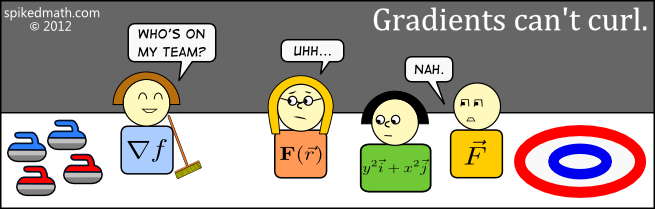
\includegraphics[width=10cm]{501-curling-with-gradients.png}
        \else
            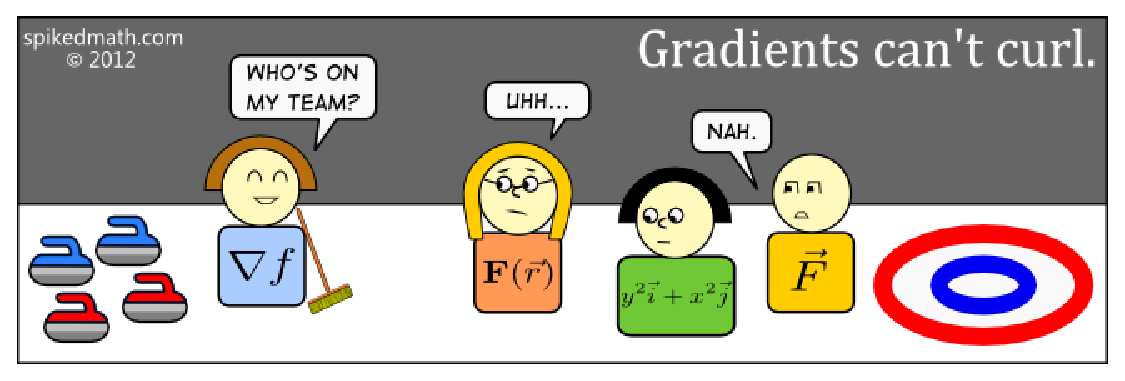
\includegraphics[width=10cm]{501-curling-with-gradients.eps}
        \fi

        {\tiny De \href{http://spikedmath.com/501.html}{Spiked math}, publié sous \href{http://creativecommons.org/licenses/by-nc-sa/2.5/ca/}{licence Creative Commons}.}
\end{center}


%+++++++++++++++++++++++++++++++++++++++++++++++++++++++++++++++++++++++++++++++++++++++++++++++++++++++++++++++++++++++++++
\section[Interprétation de la divergence]{Interprétation géométrique et physique de la divergence}
%+++++++++++++++++++++++++++++++++++++++++++++++++++++++++++++++++++++++++++++++++++++++++++++++++++++++++++++++++++++++++++


En physique, on dit qu'un champ de vecteurs à divergence nulle est \defe{incompressible}{incompressible!champ de vecteur}. Nous allons essayer de comprendre pourquoi. Lorsqu'un fluide incompressible se déplace, il faut qu'en chaque point il y autant de fluide qui rentre que de fluide qui sort. Nous allons voir sur quelques exemples que la divergence d'un champ de vecteurs est le «bilan de masse» d'un fluide qui se déplace selon le champ de vecteurs.

Si en un point la divergence est positive, cela signifie qu'il y a une perte de masse et si la divergence est négative, cela signifie qu'il y a une accumulation de masse.

Prenons par exemple un fluide qui se déplace selon le champ de vitesse montré à figure \ref{LabelFigDivergenceUn}.
\newcommand{\CaptionFigDivergenceUn}{Le champ de vecteurs $F(x,y)=\frac{1}{ x }(1,0)$.}
\input{Fig_DivergenceUn.pstricks}

Étant donné que la vitesse diminue lorsque $x$ avance, il y a une accumulation de fluide. Regardez en effet la quantité de fluide qui rentre dans le rectangle par rapport à la quantité de fluide qui en sort. Ce champ de vecteurs a pour équation :
\begin{equation}
    F(x,y)=\frac{1}{ x }\begin{pmatrix}
        1    \\ 
        0    
    \end{pmatrix}=\begin{pmatrix}
        1/x    \\ 
        0    
    \end{pmatrix}.
\end{equation}
Sa divergence vaut donc
\begin{equation}
    (\nabla\cdot F)(x,y)=\frac{ \partial F_x }{ \partial x }(x,y)+\underbrace{\frac{ \partial F_y }{ \partial y }(x,y)}_{=0}=-\frac{1}{ x^2 }.
\end{equation}
Cette divergence étant négative, il y a bien accumulation de fluide en tout point, et d'autant plus que $x$ est petit.

\begin{example}     \label{ExamDivFrotOM}

    Prenons le champ de vecteurs tournant
    \begin{equation}
        F(x,y)=\frac{1}{ \sqrt{x^2+y^2} }\begin{pmatrix}
            y    \\ 
            -x    
        \end{pmatrix}
    \end{equation}
    représenté à la figure \ref{LabelFigDivergenceDeux}. Cela est un vecteur qui est constamment perpendiculaire au rayon.

    \newcommand{\CaptionFigDivergenceDeux}{Le champ de vecteurs $F(x,y)=(y,-x)$.}
    \input{Fig_DivergenceDeux.pstricks}

    Un fluide dont la vitesse serait donné par ce champ de vecteur se contente de tourner. Intuitivement il ne devrait pas y avoir de divergence parce qu'il n'y a aucune accumulation de fluide. En effet,
    \begin{equation}
        \nabla\cdot F(x,y)=\frac{ -2xy }{ (x^2+y^2)^2 }+\frac{ 2xy }{ (x^2+y^2)^2 }=0.
    \end{equation}
\end{example}

\begin{example}
    Prenons le cas du champ de force de gravitation :
    \begin{equation}
        F(x,y,z)=\frac{1}{ (x^2+y^2+z^2)^{3/2} }\begin{pmatrix}
            x    \\ 
            y   \\
            z
        \end{pmatrix}.
    \end{equation}
    Nous pouvons rapidement remarquer que $\nabla\cdot F=0$. Est-ce que cela peut se comprendre sur le dessin de la figure \ref{LabelFigDivergenceTrois} ?
    \newcommand{\CaptionFigDivergenceTrois}{Le champ de vecteur de la gravité. Nous avons tracé, sur les deux cercles la même densité de vecteurs, c'est à dire le même nombre de vecteurs par unité de surface.}
    \input{Fig_DivergenceTrois.pstricks}

    Essayons de voir combien de fluide entre dans la zone bleue et combien en sort. D'abord, il est certain que les vecteurs qui sortent sont plus courts que ceux qui rentrent, ce qui voudrait dire qu'il y a plus de fluide qui rentre. Mais on voit également que le \emph{nombre} de vecteurs qui sortent est plus grand parce que la seconde sphère est plus grande et qu'il y a un vecteur en chaque point de la sphère.

    Intuitivement nous pouvons dire que la quantité qui rentre dans la sphère de rayon $r_1$ donnée par la taille des vecteurs entrants multiplié par la surface de la sphère, c'est à dire
    \begin{equation}        \label{EqQpinormeVectoOM}
        4\pi r_1^2\| F(x,y,z) \|,
    \end{equation}
    mais $\| F(x,y,z) \|=\frac{1}{ r_1^2 }$, donc la quantité de fluide entrant est $4\pi$. La quantité de fluide sortant sera la même.

    Cela explique deux choses
    \begin{enumerate}
        \item
            Pourquoi les forces de gravitation et électromagnétiques sont en $1/r^2$; c'est parce que nous vivons dans un monde avec trois dimensions d'espace. En étudiant très précisément le champ de gravitation, certains physiciens espèrent trouver des déviations expérimentales par rapport à la règle du \( 1/r^2\); cela \emph{pourrait} être un signe que l'espace contient des dimensions supplémentaires.
        \item
            Pourquoi il y a un $4\pi$ comme coefficient dans beaucoup d'équations en électromagnétisme; en particulier dans certaines anciennes unités de flux.
    \end{enumerate}
    
\end{example}

\begin{remark}
    Nous allons voir plus loin comment s'assurer que l'équation \eqref{EqQpinormeVectoOM} représente bien la «quantité de fluide» qui rentre dans la zone délimitée
\end{remark}


%+++++++++++++++++++++++++++++++++++++++++++++++++++++++++++++++++++++++++++++++++++++++++++++++++++++++++++++++++++++++++++
\section{Quelques formules de Leibnitz}
%+++++++++++++++++++++++++++++++++++++++++++++++++++++++++++++++++++++++++++++++++++++++++++++++++++++++++++++++++++++++++++

La divergence étant une combinaison de dérivées, il n'est pas tellement étonnant que la divergence de produits donne lieux à des formules en deux termes. Si $f$ est une fonction et si $F$ et $G$ sont des champs de vecteurs, nous avons (sans démonstrations) :
\begin{equation}        \label{EqLeinDivNablRotOM}
    \begin{aligned}[]
        \nabla\cdot(fF)&=f\nabla\cdot F+F\cdot\nabla f\\
        \nabla\cdot(F\times G)&=G\cdot\nabla\times F-F\cdot\nabla\times G.
    \end{aligned}
\end{equation}
Nous avons aussi, pour le rotationnel,
\begin{equation}        \label{EqLeinRotfFFOM}
    \nabla\times(fF)=f\nabla\times F+\nabla f\times F.
\end{equation}


\chapter{Coordonnées curvilignes orthogonales}
% This is part of Mes notes de mathématique
% Copyright (c) 2011-2012,2015
%   Laurent Claessens
% See the file fdl-1.3.txt for copying conditions.

%+++++++++++++++++++++++++++++++++++++++++++++++++++++++++++++++++++++++++++++++++++++++++++++++++++++++++++++++++++++++++++
\section{La différentielle revisitée}
%+++++++++++++++++++++++++++++++++++++++++++++++++++++++++++++++++++++++++++++++++++++++++++++++++++++++++++++++++++++++++++

%---------------------------------------------------------------------------------------------------------------------------
\subsection{Les formes différentielles de base}
%---------------------------------------------------------------------------------------------------------------------------

Si la fonction $f\colon \eR^n\to \eR$ est différentiable alors la différentielle en $a\in\eR^n$ est l'application
\begin{equation}        \label{EqFormDiffdfahOM}
    \begin{aligned}
        df_a\colon \eR^n&\to \eR \\
        u&\mapsto \frac{ \partial f }{ \partial x_1 }(a)u_1+\cdots+\frac{ \partial f }{ \partial x_n }(a)u_n.
    \end{aligned}
\end{equation}
Considérons en particulier la fonction qui à $x\in\eR^n$ fait correspondre $x_i\in\eR$. Par abus de notations,  nous la noterons $x_i$. Nous avons 
\begin{equation}
    \frac{ \partial x_i }{ \partial x_j }=\delta_{ij}.
\end{equation}
Par exemple $\partial_yx=0$ et $\partial_xx=1$. Toutes les dérivées partielles de $x_i$ s'annulent sauf la $i$ème qui vaut $1$. Par conséquent
\begin{equation}
    \begin{aligned}
        dx_i\colon \eR^n&\to \eR \\
        u&\mapsto u_i. 
    \end{aligned}
\end{equation}

\begin{remark}
    En toute rigueur nous devrions écrire $(dx_i)_a$. Mais étant donné que
    \begin{equation}
        (dx_i)_a(u)=(dx_i)_b(u)
    \end{equation}
    pour tout points $a$, $b$ et pour tout vecteurs $u$, nous nous permettons de simplifier la notation en ne précisant pas en quel point nous calculons la différentielle de $x_i$.
\end{remark}

Étant donné que $dx_i(u)=u_i$, nous pouvons récrire la formule \eqref{EqFormDiffdfahOM} en remplaçant $u_i$ par $dx_i(u)$ :
\begin{equation}
    df_a(u)=\frac{ \partial f }{ \partial x_1 }(a)dx_1(u)+\cdots+\frac{ \partial f }{ \partial x_n }(a)dx_n(u).
\end{equation}
En tant que application linéaire, $df_a$ est une combinaison linéaire des $dx_i$. En notations compacte :
\begin{equation}
    df_a=\sum_{i=1}^n\frac{ \partial f }{ \partial x_i }(a)dx_i.
\end{equation}

%---------------------------------------------------------------------------------------------------------------------------
\subsection{Différentielles de fonctions composées}
%---------------------------------------------------------------------------------------------------------------------------

Cette façon de voir la différentielle nous permet de jeter un nouveau regard sur la formule de différentiation des fonctions composées. Soient
\begin{equation}
    \begin{aligned}[]
        f\colon \eR^p&\to \eR^n\\
        g\colon \eR^n&\to \eR,
    \end{aligned}
\end{equation}
et $h\colon \eR^p\to \eR$ définie par 
\begin{equation}
    h(u)=h\big( f(u) \big)=(g\circ f)(u).
\end{equation}
Nous allons noter $x$ les coordonnées de $\eR^p$, $a$ un point de $\eR^p$ et $u$, un vecteur de $\eR^p$ accroché au point $a$. Pour $\eR^n$, les notations seront que les coordonnées sont $y$, $b$ est un point de $\eR^n$ et $v$ est un vecteur «accroché» au point $b$.

Nous avons
\begin{equation}
    dg_b(v)=\sum_{i=1}^n\frac{ \partial g }{ \partial y_i }(b)dy_i(v).
\end{equation}
Ici $dy_i(v)$ signifie la $i$ème composante de $v$. C'est simplement $v_i$. Cette formule étant valable pour tout point $b\in\eR^n$ et pour tout vecteur $v$, nous pouvons l'écrire en particulier pour
\begin{subequations}
    \begin{numcases}{}
        b=f(a)\\
        v=df_a(u).
    \end{numcases}
\end{subequations}
Cela donne
\begin{equation}        \label{EqdgfadfauOM}
    dg_{f(a)}\big( df_a(u) \big)=\sum_{i=1}^n\frac{ \partial g }{ \partial y_i }\big( f(a) \big)dy_i\big( df_a(u) \big).
\end{equation}
Mais 
\begin{equation}
    df_a(u)=\sum_{j=1}^p\frac{ \partial f }{ \partial x_j }(a)dx_j(u),
\end{equation}
donc la $i$ème composante de ce vecteur est
\begin{equation}
     \big( df_a(u)\big)_i=\sum_{j=1}^p\frac{ \partial f_i }{ \partial x_j }(a)dx_j(u).
\end{equation}
En remplaçant $dy_i\big( df_a(u) \big)$ par cela dans l'expression \eqref{EqdgfadfauOM}, nous trouvons
\begin{equation}
    dg_{f(a)}\big( df_a(u) \big)=\sum_{i=1}^n\frac{ \partial g }{ \partial y_i }\big( f(a) \big)\sum_{j=1}^p\frac{ \partial f_i }{ \partial x_j }(a)dx_j(u).
\end{equation}
Nous pouvons vérifier que cela est la différentielle de $g\circ f$ au point $a$ appliquée au vecteur $u$. En effet
\begin{equation}
    d(g\circ f)_a(u)=\sum_{j=1}^p\frac{ \partial (g\circ f) }{ \partial x_j }(a)dx_j(u),
\end{equation}
tandis que, par la dérivation de fonctions composées, 
\begin{equation}        \label{EqDerCompofgOM}
    \frac{ \partial (g\circ f) }{ \partial x_j }(a)=\sum_{i=1}^n\frac{ \partial g }{ \partial y_i }\big( f(a) \big)\frac{ \partial f_i }{ \partial x_j }(a).
\end{equation}
Au final, ce que nous avons prouvé est que
\begin{equation}
    d(g\circ f)_a(u)=dg_{f(a)}\big( df_a(u) \big).
\end{equation}

%---------------------------------------------------------------------------------------------------------------------------
\subsection{Passage aux coordonnées polaires}
%---------------------------------------------------------------------------------------------------------------------------

Le changement de coordonnées pour les polaires est la fonction
\begin{equation}
    f\begin{pmatrix}
        r    \\ 
        \theta    
    \end{pmatrix}=\begin{pmatrix}
        x    \\ 
        y    
    \end{pmatrix}=\begin{pmatrix}
        r\cos\theta    \\ 
        r\sin\theta    
    \end{pmatrix}.
\end{equation}
Considérons une fonction $g$ sur $\eR^2$, et définissons la fonction $\tilde g$ par
\begin{equation}
    \tilde g(r,\theta)=g(r\cos\theta,r\sin\theta).
\end{equation}
La formule \eqref{EqDerCompofgOM} permet de trouver les dérivées partielles de $g$ par rapport à $r$ et $\theta$ en termes de celles par rapport à $x$ et $y$ de $g$.

Pour faire le lien avec les notations du point précédent, nous avons
\begin{equation}
    \begin{aligned}[]
        f_1(r,\theta)&=r\cos(\theta)\\
        f_2(r,\theta)&=r\sin(\theta)\\
        (x_1,x_2)&\to(r,\theta)\\
        (y_1,y_2)&\to(x,y).
    \end{aligned}
\end{equation}
Nous avons donc 
\begin{equation}
    \begin{aligned}[]
        \frac{ \partial \tilde g }{ \partial r }(r,\theta)&=\sum_{i=1}^2\frac{ \partial g }{ \partial x_i }\big( f(r,\theta) \big)\frac{ \partial f_i }{ \partial r }(r,\theta)\\
        &=\frac{ \partial g }{ \partial x }(r\cos\theta,r\sin\theta)\frac{ \partial \big( r\cos\theta \big) }{ \partial r }(r,\theta)\\
        &\quad+\frac{ \partial g }{ \partial y }(r\cos\theta,r\sin\theta)\frac{ \partial \big( r\sin\theta\big) }{ \partial r }(r,\theta)\\
        &=\cos\theta\frac{ \partial g }{ \partial x }(r\cos\theta,r\sin\theta)+\sin\theta\frac{ \partial g }{ \partial y }(r\cos\theta,r\sin\theta).
    \end{aligned}
\end{equation}

Prenons par exemple $g(x,y)=\frac{1}{ x^2+y^2 }$. Étant donné que
\begin{equation}
    \frac{ \partial g }{ \partial x }=\frac{ -2x }{ (x^2+y^2)^2 },
\end{equation}
nous avons
\begin{equation}
    \frac{ \partial g }{ \partial x }(r\cos\theta,r\sin\theta)=\frac{ -2\cos\theta }{ r^3 }.
\end{equation}
En utilisant la formule,
\begin{equation}
    \frac{ \partial \tilde g }{ \partial r }(r,\theta)=\cos(\theta)\left( \frac{ -2\cos\theta }{ r^3 } \right)+\sin(\theta)\left( \frac{ -2\sin\theta }{ r^3 } \right)=-\frac{ 2 }{ r^3 }.
\end{equation}
Nous pouvons vérifier directement que cela est correct. En effet
\begin{equation}
    \tilde g(r,\theta)=g(r\cos\theta,r\sin\theta)=\frac{1}{ r^2 },
\end{equation}
dont la dérivée par rapport à $r$ vaut $-2/r^3$.

En ce qui concerne la dérivée par rapport à $\theta$, nous avons
\begin{equation}
    \begin{aligned}[]
    \frac{ \partial \tilde g }{ \partial \theta }&=\frac{ \partial g }{ \partial x }(r\cos\theta,r\sin\theta)\frac{ \partial \big( r\cos(\theta) \big) }{ \partial \theta }+\frac{ \partial g }{ \partial y }(r\cos\theta,r\sin\theta)\frac{ \partial \big( r\sin(\theta) \big) }{ \partial \theta }\\
    &=\left( \frac{ -2\cos\theta }{ r^3 } \right)(-r\sin\theta)+\left( \frac{ -2\sin\theta }{ r^3 } \right)(r\cos\theta)\\
    &=0.
    \end{aligned}
\end{equation}

En résumé et avec quelques abus de notations :
\begin{equation}
    \begin{aligned}[]
        \frac{ \partial \tilde g }{ \partial r }&=\cos(\theta)\frac{ \partial g }{ \partial x }+\sin(\theta)\frac{ \partial g }{ \partial y }\\
        \frac{ \partial \tilde g }{ \partial \theta }&=-r\sin(\theta)\frac{ \partial g }{ \partial x }+r\cos(\theta)\frac{ \partial g }{ \partial y }\\
    \end{aligned}
\end{equation}

%+++++++++++++++++++++++++++++++++++++++++++++++++++++++++++++++++++++++++++++++++++++++++++++++++++++++++++++++++++++++++++
\section{Théorie générale}
%+++++++++++++++++++++++++++++++++++++++++++++++++++++++++++++++++++++++++++++++++++++++++++++++++++++++++++++++++++++++++++

%---------------------------------------------------------------------------------------------------------------------------
\subsection{Base locale}
%---------------------------------------------------------------------------------------------------------------------------

Les coordonnées sphériques et cylindriques sont deux systèmes de coordonnées «un peu courbe» qui existent sur $\eR^3$. Il en existe de nombreux autres, que nous appelons \defe{coordonnées curvilignes}{coordonnées!curvilignes}. Des coordonnées curvilignes sur $\eR^3$ est n'importe quel\footnote{Nous n'entrons pas dans les détails de régularité.} système qui permet de repérer un point de $\eR^3$ à partir de trois nombres.

Il s'agit donc d'un ensemble de trois applications 
\begin{equation}
    x_i\colon \eR^3\to \eR.
\end{equation}
Les coordonnées cylindriques sont
\begin{subequations}
    \begin{numcases}{}
        x_1(r,\theta,z)=r\cos\theta\\
        x_2(r,\theta,z)=r\sin\theta\\
        x_3(r,\theta,z)=z
    \end{numcases}
\end{subequations}

Soit donc un système général $q=(q_1,q_2,q_3)$ et 
\begin{equation}
    M(q)=\begin{pmatrix}
        x_1(q)    \\ 
        x_2(q)    \\ 
        x_3(q)    
    \end{pmatrix}.
\end{equation}
Si nous fixons $q_2$ et $q_3$ et que nous laissons varier $q_1$, nous obtenons une courbe\footnote{Dans le cas des sphériques, c'est une demi-droite horizontale d'angle $q_2$ et de hauteur $q_3$.} dont nous pouvons considérer le vecteur vitesse, c'est à dire le vecteur tangent. En chaque point nous avons ainsi trois vecteurs
\begin{equation}
    \frac{ \partial M }{ \partial q_i }(q).
\end{equation}
Nous disons que le système de coordonnées curviligne est \defe{orthogonal}{orthogonal!coordonnées curviligne} si ces trois vecteurs sont orthogonaux. Dans la suite nous supposerons que c'est toujours le cas.

Nous posons
\begin{equation}
    h_i=\left\| \frac{ \partial M }{ \partial q_i } \right\|
\end{equation}
et nous considérons les trois vecteurs normés
\begin{equation}        \label{EqDefeihMqOM}
    e_i=h_i^{-1}\frac{ \partial M }{ \partial q_i }.
\end{equation}
Les trois vecteurs $\{ e_1,e_2,e_3 \}$ forment une base orthonormée dite \defe{base locale}{base!locale}. Ce sont des vecteurs liés\footnote{En géométrie différentielle on dira que ce sont des élément de l'espace tangent, mais c'est une toute autre histoire.} au point $M$.

%---------------------------------------------------------------------------------------------------------------------------
\subsection{Importance de l'orthogonalité}
%---------------------------------------------------------------------------------------------------------------------------

Nous avons dit que nous nous restreignons au cas où les vecteurs $e_i$ sont orthogonaux. En termes de produits scalaires, cela signifie
\begin{equation}
    e_i\cdot e_j=\delta_{ij}.
\end{equation}
Nous en étudions maintenant quelque conséquence. L'équation \eqref{EqDefeihMqOM} peut s'écrire plus explicitement sous la forme
\begin{equation}
    e_i=\sum_k h_i^{-1}\frac{ \partial x_k }{ \partial q_i }1_k.
\end{equation}
Notez que pour chaque $k$ et $i$, la quantité $h_i^{-1}\frac{ \partial x_k }{ \partial q_i }$ est un simple nombre. Nous allons les mettre dans une matrice :
\begin{equation}
    A_{ki}=h_i^{-1}\frac{ \partial x_k }{ \partial q_i }.
\end{equation}
Cela nous donne le changement de base
\begin{equation}        \label{EqChmBaseeisAkiAkOM}
    e_i=\sum_kA_{ki}1_k.
\end{equation}
Le produit $e_i\cdot e_j$ s'écrit alors
\begin{equation}
    \begin{aligned}[]
        e_i\cdot e_j&=\sum_{kl}A_{ki}A_{lj}\underbrace{1_k\cdot 1_l}_{=\delta_{kl}}\\
        &=\sum_{kl}A_{ki}A_{lj}\delta_{kl}\\
        &=\sum_kA_{ki}A_{kj}\\
        &=\sum_k(A^T)_{ik}A_{kj}.
    \end{aligned}
\end{equation}
Or cela doit valoir $\delta_{ij}$. Par conséquent 
\begin{equation}
    A^T=A^{-1}.
\end{equation}
Le fait que les coordonnées curvilignes considérées soient orthogonales s'exprime donc par la fait que la matrice de changement de base est une matrice orthogonale.

Cette circonstance nous permet d'inverser le changement de base \eqref{EqChmBaseeisAkiAkOM} en multipliant cette équation par $(A^{-1})_{il}$ des deux côtés et en faisant la somme sur $i$ :
\begin{equation}
    \sum_i (A^{-1})_{il}e_i=\sum_{kl}\underbrace{A_{ki}(A^{-1})_{il}}_{=\delta_{kl}}1_k,
\end{equation}
par conséquent
\begin{equation}
    \sum_i(A^T)_{il}e_i=1_l,    
\end{equation}
et
\begin{equation}        \label{EqChamvarunlAeiOM}
    1_l=\sum_iA_{li}e_i=\sum_ih_i^{-1}\frac{ \partial x_l }{ \partial q_i }e_i.
\end{equation}
Armés de cette importante formule, nous pouvons exprimer les quantités que nous connaissons dans la base canonique en termes de la base locale.

Une autre conséquence du fait que $e_1$, $e_2$ et $e_3$ est une base orthonormée est que, éventuellement en réordonnant les vecteurs, on a
\begin{equation}
    \begin{aligned}[]
        e_1\times e_2&=e_3\\
        e_2\times e_3&=e_1\\
        e_3\times e_1&=e_2
    \end{aligned}
\end{equation}
Ces trois relations s'écrivent en une seule avec
\begin{equation}
    e_i\times e_j=\sum_{k}\epsilon_{ijk}e_k
\end{equation}
où 
\begin{equation}
    \epsilon_{ijk}=\begin{cases}
        0    &   \text{si} i,j,k \text{ne sont pas tous différents}\\
        1    &    \text{si } ijk \text{ se ramène à 123 par un nombre pair de permutations}\\
        -1    &    \text{si }ijk \text{ se ramène à 123 par un nombre impair de permutations}
    \end{cases}
\end{equation}
est le \defe{symbole de Levi-Civita}{Levi-Civita}. La formule du produit vectoriel peut également être utilisée à l'envers sous la forme
\begin{equation}        \label{EqekeitimesejOM}
    e_k=\frac{ 1 }{2}\sum_{ij}\epsilon_{ijk}\,e_i\times e_j.
\end{equation}

Le symbole de Levi-Civita possède de nombreuses formules. En voici certaines, facilement démontrables en considérant tous les cas :
\begin{equation}
    \epsilon_{ijk}\epsilon_{ijl}=\delta_{kl}| \epsilon_{ijk} |.
\end{equation}
Grâce au symboles de Levi-Civita, le produit mixte des vecteurs de base a une belle forme :
\begin{equation}        \label{EqProdMixteepsilonCicivrOM}
    e_l\cdot(e_i\times e_j)=\sum_k\epsilon_{ijk}e_l\times e_k=\sum_k\epsilon_{ijk}\delta_{lk}=\epsilon_{ijl}.
\end{equation}

%+++++++++++++++++++++++++++++++++++++++++++++++++++++++++++++++++++++++++++++++++++++++++++++++++++++++++++++++++++++++++++
\section{Gradient en coordonnées curvilignes}
%+++++++++++++++++++++++++++++++++++++++++++++++++++++++++++++++++++++++++++++++++++++++++++++++++++++++++++++++++++++++++++

Soit $(x,y,z)\mapsto f(x,y,z)$ une fonction sur $\eR^3$. Nous pouvons la composer avec les coordonnées curvilignes $q$ pour obtenir la fonction
\begin{equation}
    \tilde f(q_1,q_2,q_3)=f\big( x_1(q),x_2(x),x_3(q) \big).
\end{equation}
Nous disons que $\tilde f$ est l'expression de $f$ dans les coordonnées $q$. Nous savons déjà comment calculer le gradient de $f$ en coordonnées cartésiennes :
\begin{equation}
    F(x,y, z)=\nabla f(x,y,z)=\begin{pmatrix}
        \partial_xf(x,y,z)    \\ 
        \partial_yf(x,y,z)    \\ 
        \partial_zf(x,y,z)    \
    \end{pmatrix}.
\end{equation}
Cela est un vecteur lié au point $(x,y,z)$. Nous voudrions exprimer ce vecteur dans la base $\{ e_1,e_2,e_3 \}$. En d'autres termes, nous voudrions trouver les nombres $\tilde F_1$, $\tilde F_2$ et $\tilde F_3$ tels que
\begin{equation}
    F(x,y,z)=F\big( x(q),y(q),z(q) \big)=\tilde F_1e_1+\tilde F_2e_2+\tilde F_3e_3.
\end{equation}
Ces nombres seront des fonctions de $(q_1,q_2,q_3)$.

Par définition,
\begin{equation}
    \nabla f=\sum_l\frac{ \partial f }{ \partial x_l }1_l.
\end{equation}
En remplaçant $1_l$ par sa valeur en termes des $e_i$ par la formule \eqref{EqChamvarunlAeiOM},
\begin{equation}
    \begin{aligned}[]
        \nabla f&=\sum_l\frac{ \partial f }{ \partial x_l }1_l\\
        &=\sum_l\frac{ \partial f }{ \partial x_l }\sum_ih_i^{-1}\frac{ \partial x_l }{ \partial q_i }e_i\\
        &=\sum_{il}\frac{1}{ h_i }\frac{ \partial f }{ \partial x_l }\frac{ \partial x_l }{ \partial q_i }e_i\\
        &=\sum_i\frac{1}{ h_i }\frac{ \partial \tilde f }{ \partial q_i }e_i.
    \end{aligned}
\end{equation}

Plus explicitement,
\begin{equation}        \label{EqGradientenCurviligneOM}
    \nabla f\big( x(q),y(q),z(q) \big)=\sum_i \frac{1}{ h_i(q) }\frac{ \partial \tilde f }{ \partial q_i }(q)e_i
\end{equation}
où
\begin{equation}
    h_i(q)=\left\| \frac{ \partial M }{ \partial q_i }(q) \right\|.
\end{equation}
Le plus souvent nous n'allons pas noter explicitement la dépendance de $h_i$ en $q$.

Quelques formulaires intéressants sont en appendice de \cite{Schomblond_em}.

%---------------------------------------------------------------------------------------------------------------------------
\subsection{Coordonnées polaires}
%---------------------------------------------------------------------------------------------------------------------------

Les coordonnées curvilignes polaires sont données par
\begin{equation}
    M(r,\theta)=\begin{pmatrix}
        r\cos(\theta)    \\ 
        r\sin(\theta)    
    \end{pmatrix},
\end{equation}
et par conséquent
\begin{equation}
    \begin{aligned}[]
        \frac{ \partial M }{ \partial r }&=\begin{pmatrix}
            \cos(\theta)    \\ 
            \sin(\theta)    
        \end{pmatrix},&\frac{ \partial M }{ \partial \theta }=\begin{pmatrix}
            -r\sin(\theta)    \\ 
            r\cos(\theta)    
        \end{pmatrix}.
    \end{aligned}
\end{equation}
Nous avons les normes $h_r=1$ et $h_{\theta}=r$, et donc les vecteurs de la base locale en $(r,\theta)$ sont
\begin{equation}
    e_r=\begin{pmatrix}
        \cos(\theta)    \\ 
        \sin(\theta)    
    \end{pmatrix}=\cos(\theta)e_x+\sin(\theta)e_y
\end{equation}
ainsi que
\begin{equation}
    e_{\theta}=\begin{pmatrix}
        -\sin(\theta)    \\ 
        \cos(\theta)    
    \end{pmatrix}=-\sin(\theta)e_x+\cos(\theta)e_y.
\end{equation}


Ces vecteurs sont représentés à la figure \ref{LabelFigCurvilignesPolaires}. Notez qu'il y en a une paire différente en chaque point.
\newcommand{\CaptionFigCurvilignesPolaires}{En brun, les lignes que le point suivrait si on ne variait qu'une coordonnées polaire à la fois. Les vecteurs rouges sont les vecteurs $e_{r}$ et $e_{\theta}$.}
\input{pictures_tex/Fig_CurvilignesPolaires.pstricks}


%---------------------------------------------------------------------------------------------------------------------------
\subsection{Coordonnées cylindriques}
%---------------------------------------------------------------------------------------------------------------------------

Les coordonnées cylindriques sont les mêmes que les coordonnées polaires à part qu'il faut écrire
\begin{equation}
    M(r,\theta,z)=\begin{pmatrix}
        r\cos(\theta)    \\ 
        r\sin(\theta)    \\ 
        z    
    \end{pmatrix},
\end{equation}
et nous avons le vecteur de base supplémentaire
\begin{equation}
    e_z=\frac{ \partial M }{ \partial z }=\begin{pmatrix}
        0    \\ 
        0    \\ 
        1    
    \end{pmatrix}
\end{equation}
parce que $h_z=1$.

%---------------------------------------------------------------------------------------------------------------------------
\subsection{Coordonnées sphériques}
%---------------------------------------------------------------------------------------------------------------------------

Les coordonnées curvilignes sphériques sont données par
\begin{equation}
    M(\rho,\theta,\varphi)=
    \begin{pmatrix}
        \rho\sin(\theta)\cos(\varphi)    \\ 
        \rho\sin(\theta)\sin(\varphi)    \\ 
        \rho\cos(\theta)
    \end{pmatrix},
\end{equation}
dont les dérivées sont données par
\begin{equation}
    \begin{aligned}[]
        \frac{ \partial M }{ \partial r }&=\begin{pmatrix}
        \sin(\theta)\cos(\varphi)    \\ 
        \sin(\theta)\sin(\varphi)    \\ 
        \cos(\theta)
    \end{pmatrix},
    &\frac{ \partial M }{ \partial \theta }&=
    \begin{pmatrix}
        \rho\cos(\theta)\cos(\varphi)    \\ 
        \rho\cos(\theta)\sin(\varphi)    \\ 
        -\rho\sin(\theta)
    \end{pmatrix},\\
    \frac{ \partial M }{ \partial \varphi }&=
    \begin{pmatrix}
        -\rho\sin(\theta)\sin(\varphi)    \\ 
        \rho\sin(\theta)\cos(\varphi)    \\ 
        0
    \end{pmatrix}
    \end{aligned}
\end{equation}
Les normes de ces vecteurs sont $h_{\rho}=1$, $h_{\theta}=\rho$ et $h_{\varphi}=\rho\sin(\theta)$. Les vecteurs de la base locale en $(\rho,\theta,\varphi)$ sont donc
\begin{equation}
    \begin{aligned}[]
        e_r&=\begin{pmatrix}
        \sin(\theta)\cos(\varphi)    \\ 
        \sin(\theta)\sin(\varphi)    \\ 
        \cos(\theta)
    \end{pmatrix},
    &e_{\theta}&=
    \begin{pmatrix}
        \cos(\theta)\cos(\varphi)    \\ 
        \cos(\theta)\sin(\varphi)    \\ 
        -\sin(\theta)
    \end{pmatrix},\\
    e_{\varphi}&=
    \begin{pmatrix}
        -\sin(\varphi)    \\ 
        \cos(\varphi)    \\ 
        0
    \end{pmatrix}
    \end{aligned}
\end{equation}

Nous pouvons exprimer le gradient d'une fonction en coordonnées sphériques en utilisant la formule \eqref{EqGradientenCurviligneOM} :
\begin{equation}        \label{EqGradientSpheriqueOM}
    \nabla\tilde f(\rho,\theta,\varphi)=\frac{ \partial \tilde f }{ \partial \rho }e_{\rho}+\frac{1}{ \rho }\frac{ \partial \tilde f }{ \partial \theta }e_{\theta}+\frac{1}{ \rho\sin(\theta) }\frac{ \partial \tilde f }{ \partial \varphi }r_{\varphi}.
\end{equation}
Cette expression peut paraître peu pratique parce que les vecteurs $e_{\rho}$, $e_{\theta}$ et $e_{\varphi}$ eux-mêmes changent en chaque point. Elle est effectivement peu adaptée au dessin, mais elle est très pratique pour des fonctions ayant des symétries.

\begin{example}
    Le potentiel de la gravitation est la fonction
    \begin{equation}
        V(x,y,z)=\frac{1}{ \sqrt{x^2+y^2+z^2} }.
    \end{equation}
    En coordonnées sphériques elle s'écrit
    \begin{equation}
        \tilde V(\rho,\theta,\varphi)=\frac{1}{ \rho }.
    \end{equation}
    En voila une fonction qu'elle est facile à dériver, contrairement à $V$ ! En suivant la formule \eqref{EqGradientSpheriqueOM}, nous avons immédiatement
    \begin{equation}
        \nabla\tilde V=-\frac{1}{ \rho^2 }e_{\rho}.
    \end{equation}
    Nous voyons immédiatement que cela est un champ de vecteurs dont la norme diminue comme le carré de la distance à l'origine et qui est en permanence dirigé vers l'origine.
\end{example}


%+++++++++++++++++++++++++++++++++++++++++++++++++++++++++++++++++++++++++++++++++++++++++++++++++++++++++++++++++++++++++++
\section{Divergence en coordonnées curvilignes}
%+++++++++++++++++++++++++++++++++++++++++++++++++++++++++++++++++++++++++++++++++++++++++++++++++++++++++++++++++++++++++++

Nous savons que 
\begin{equation}
    \nabla\tilde f=\sum_j\frac{1}{ h_j }\frac{ \partial \tilde f }{ \partial q_j }e_j.
\end{equation}
Nous pouvons en particulier considérer la fonction $f(q)=q_i$. De la même manière que nous avions noté $x_i$ la fonction $x\mapsto x_i$, nous notons $q_i$ la fonction $q\mapsto q_i$. Le gradient de cette fonction est donné par
\begin{equation}
    \nabla q_i=\sum_j\frac{1}{ h_j }\frac{ \partial q_i }{ \partial q_j }e_j,
\end{equation}
mais $\frac{ \partial q_i }{ \partial q_j }=\delta_{ij}$, donc
\begin{equation}
    \nabla q_i=\frac{ e_i }{ h_i },
\end{equation}
ou encore
\begin{equation}
    e_i=h_i\nabla q_i.
\end{equation}
Cela n'est pas étonnant : la direction dans laquelle la coordonnées $q_i$ varie le plus est le vecteur $e_i$ qui donne la tangente à la courbe obtenue lorsque \emph{seul} $q_i$ varie.

Commençons par calculer la divergence de $e_i$. En utilisant la formule \eqref{EqekeitimesejOM},
\begin{equation}
    \nabla\cdot e_k=\frac{ 1 }{2}\sum_{ij}\epsilon_{ijk}\,\nabla\cdot (e_i\times e_j).
\end{equation}
Nous avons, en utilisant les règles de Leibnitz \eqref{EqLeinDivNablRotOM}, 
\begin{equation}
    \begin{aligned}[]
        \nabla\cdot(e_i\times e_j)&=\nabla\cdot(h_i\nabla q_i\times h_j\nabla q_j)\\
        &=\nabla(h_ih_j)\cdot\big( \nabla q_i\times\nabla q_j \big)+h_ih_j\nabla\cdot\big( \nabla q_i\times\nabla q_j \big)\\
        &=\nabla(h_ih_j)\cdot\big( \nabla q_i\times\nabla q_j \big)\\
        &\quad+h_ih_j\nabla q_j\cdot\big( \underbrace{\nabla\times\nabla q_i}_{=0} \big)\\
        &\quad+h_ih_j\nabla q_i\cdot\big( \underbrace{\nabla\times\nabla q_j}_{=0} \big)
    \end{aligned}
\end{equation}
Cela nous fait
\begin{equation}
    \nabla\cdot e_k=\sum_{ij}\epsilon_{ijk}\frac{ \nabla(h_ih_j) }{ h_ih_j }\cdot (e_i\times e_j).
\end{equation}
parce que $\nabla q_i=h_i^{-1}e_i$. Nous pouvons développer le gradient qui intervient :
\begin{equation}
    \nabla(h_ih_j)=\sum_l\frac{1}{ h_l }\frac{ \partial  }{ \partial q_l }(h_ih_j)e_l.
\end{equation}
Nous voyons donc arriver le produit mixte $e_l\cdot (e_i\times e_j)$. En utilisant la formule \eqref{EqProdMixteepsilonCicivrOM}, cela s'exprime directement sous la forme $\epsilon_{ijl}$.

Nous avons alors
\begin{equation}        \label{EqFragradekdviOM}
    \begin{aligned}[]
        \nabla\cdot e_k&=\frac{ 1 }{2}\sum_{ijl}\frac{1}{ h_ih_jh_l }\frac{ \partial  }{ \partial q_l }(h_ih_j)\epsilon_{ijk}\epsilon_{ijl}\\
        &=\frac{ 1 }{2}\sum_{ijl}\delta_{kl}| \epsilon_{ijk} |\frac{ \partial  }{ \partial q_l }(h_ih_j)\\
        &=\frac{ 1 }{2}\sum_{ij}\frac{| \epsilon_{ijk} |}{ h_ih_jh_k }\frac{ \partial  }{ \partial q_k }(h_ih_j).
    \end{aligned}
\end{equation}
Par exemple,
\begin{equation}
    \nabla\cdot e_1=\frac{1}{ h_1h_2h_3 }\frac{ \partial  }{ \partial q_1 }(h_2h_3).
\end{equation}

Nous devons maintenant chercher le gradient d'un champ général
\begin{equation}
    F(q)=\sum_kF_k(q)e_k.
\end{equation}
La première chose à faire est d'utiliser la formule de Leibnitz :
\begin{equation}        \label{EqLeibnbablaFekOM}
    \nabla\cdot F=\sum_k\nabla F_k(q)\cdot e_k+\sum_kF_k(q)\nabla\cdot e_k.
\end{equation}
Afin d'alléger les notations, nous allons nous concentrer sur le terme numéro $k$ et ne pas écrire la somme. Si $i$ et $j$ sont les nombres tels que $\epsilon_{ijk}=1$, alors ce que la formule \eqref{EqFragradekdviOM} signifie, c'est que
\begin{equation}
    \nabla\cdot e_k=\frac{1}{ h_1h_2h_3 }\frac{ \partial  }{ \partial q_k }(h_ih_j).
\end{equation}
Nous savons déjà par la formule \eqref{EqGradientenCurviligneOM} que
\begin{equation}
    \nabla F_k=\sum_l\frac{1}{ h_l }\frac{ \partial F_k }{ \partial q_l }e_l,
\end{equation}
par conséquent
\begin{equation}
    \nabla F_k\cdot e_k=\sum_l\frac{1}{ h_l }\frac{ \partial F_k }{ \partial q_l }\delta_{kl}=\frac{1}{ h_k }\frac{ \partial F_k }{ \partial q_k }.
\end{equation}
Pour obtenir cela nous avons utilisé le fait que $e_l\cdot e_k=\delta_{lk}$. Le terme numéro $k$ de la somme \eqref{EqLeibnbablaFekOM} est donc
\begin{equation}
    \frac{1}{ h_k }\frac{ \partial F_k }{ \partial q_k }+\frac{ F_k }{ h_kh_ih_j }\frac{ \partial (h_ih_j) }{ \partial q_k }=\frac{1}{ h_ih_jh_k }\frac{ \partial (F_kh_ih_j) }{ \partial q_k }
\end{equation}
où il est entendu que $i$ et $j$ représentent les nombres tels que $\epsilon_{ijk}=1$.

Au final, nous avons
\begin{equation}
    \nabla\cdot F=\frac{1}{ h_1h_2h_3 }\sum_{ijk}| \epsilon_{ijk} |\frac{ \partial (F_kh_ih_j) }{ \partial q_k }.
\end{equation}
Ici, la somme sur $i$ et $j$ consiste seulement à sélectionner les termes tels que $i$ et $j$ ne sont pas $k$. En écrivant la somme explicitement,
\begin{equation}
    \begin{aligned}[]
        \nabla\cdot F=\frac{1}{ h_1h_2h_3 }\left[ \frac{ \partial  }{ \partial q_1 }(F_1h_2h_3)+\frac{ \partial  }{ \partial q_2 }(F_2h_1h_3)+\frac{ \partial  }{ \partial q_3 }(F_3h_1h_2) \right].
    \end{aligned}
\end{equation}

%---------------------------------------------------------------------------------------------------------------------------
\subsection{Coordonnées cylindriques}
%---------------------------------------------------------------------------------------------------------------------------

En coordonnées cylindriques, nous avons déjà vu que $h_r=1$, $h_{\theta}=r$ et $h_z=1$. La divergence est donc donnée par
\begin{equation}        \label{EqDivEnCylonfOM}
    \nabla\cdot F=\frac{1}{ r }\left[ \frac{ \partial  }{ \partial r }(rF_r)+\frac{ \partial  }{ \partial \theta }(F_{\theta})+\frac{ \partial  }{ \partial z }(rF_z) \right].
\end{equation}
Par exemple si
\begin{equation}
    F(r,\theta,z)=re_{\theta}+e_z,
\end{equation}
nous avons
\begin{equation}
    (\nabla\cdot F)(r,\theta,z)=\frac{1}{ r }\left[ \frac{ \partial  }{ \partial \theta }(r)+\frac{ \partial  }{ \partial z }(r) \right]=0.
\end{equation}
Cela est logique parce que $re_{\theta}$ est à peu près le champ dont nous avons parlé dans l'exemple \eqref{ExamDivFrotOM}, qui était à divergence nulle. En réalité, le champ dont on parlait dans cet exemple était exactement $-e_{\theta}$. Le champ $e_z$ est également à divergence nulle parce qu'il est constant.

%---------------------------------------------------------------------------------------------------------------------------
\subsection{Coordonnées sphériques}
%---------------------------------------------------------------------------------------------------------------------------

En coordonnées sphériques, nous avons $h_{\rho}=1$, $h_{\theta}=r$ et $h_{\varphi}=r\sin\theta$, donc
\begin{equation}
    \nabla\cdot F=\frac{1}{ r^2\sin\theta }\left[ \frac{ \partial  }{ \partial \rho }(\rho^2\sin\theta F_{\rho})+\frac{ \partial  }{ \partial \theta }(\rho\sin\theta F_{\theta})+\frac{ \partial  }{ \partial \varphi }(\rho F_{\varphi}) \right].
\end{equation}
si $F(\rho,\theta,\varphi)=F_{\rho}e_{\rho}+F_{\theta}e_{\theta}+F_{\varphi}e_{\varphi}$.

%+++++++++++++++++++++++++++++++++++++++++++++++++++++++++++++++++++++++++++++++++++++++++++++++++++++++++++++++++++++++++++
\section{Laplacien en coordonnées curvilignes orthogonales}
%+++++++++++++++++++++++++++++++++++++++++++++++++++++++++++++++++++++++++++++++++++++++++++++++++++++++++++++++++++++++++++

Soit une fonction $f\colon \eR^3\to \eR$. Le \defe{Laplacien}{Laplacien} de $f$ est donné par
\begin{equation}
    \Delta f=\nabla\cdot(\nabla f).
\end{equation}
En utilisant les formules données, nous avons
\begin{equation}
    \Delta f=\frac{1}{ h_1h_2h_3 }\left[ \frac{ \partial  }{ \partial q_1 }\left( \frac{ h_2h_3 }{ h_1 }\frac{ \partial f }{ \partial q_1 } \right)  +\frac{ \partial  }{ \partial q_2 }\left( \frac{ h_1h_3 }{ h_2 }\frac{ \partial f }{ \partial q_2 } \right)  +\frac{ \partial  }{ \partial q_3 }\left( \frac{ h_1h_2 }{ h_3 }\frac{ \partial f }{ \partial q_3 } \right)     \right].
\end{equation}
Dans cette expression, la fonction $f$ est donnée comme fonction de $q_1$, $q_2$ et $q_3$.

En coordonnées cylindriques, cela s'écrit
\begin{equation}
    \begin{aligned}[]
        \Delta f&=\frac{1}{ r }\left[ \frac{ \partial  }{ \partial r }\left( r\frac{ \partial f }{ \partial r } \right)+\frac{ \partial  }{ \partial \theta }\left( \frac{1}{ r }\frac{ \partial f }{ \partial \theta } \right)+\frac{ \partial  }{ \partial z }\left( r\frac{ \partial f }{ \partial z } \right) \right]\\
        &=\frac{ \partial^2f  }{ \partial r^2 }+\frac{1}{ r }\frac{ \partial f }{ \partial r }+\frac{1}{ r^2 }\frac{ \partial^2f }{ \partial \theta^2 }+\frac{ \partial^2f }{ \partial z^2 }.
    \end{aligned}
\end{equation}
Dans cette expression, $f$ est fonction de $r$, $\theta$ et $z$.

En coordonnées sphériques, cela devient
\begin{equation}        \label{EqLaplaceSpheOM}
    \Delta f=\frac{1}{ \rho^2\sin\theta }\left[ \frac{ \partial  }{ \partial \rho }\left( \rho^2\sin\theta\frac{ \partial f }{ \partial \rho } \right)+\frac{ \partial  }{ \partial \theta }\left( \sin\theta\frac{ \partial f }{ \partial \theta } \right)+\frac{ \partial  }{ \partial \varphi }\left( \frac{1}{ \sin\theta }\frac{ \partial f }{ \partial \varphi } \right) \right].
\end{equation}
Dans cette expression, $f$ est fonction de $\rho$, $\theta$ et $\varphi$.

%+++++++++++++++++++++++++++++++++++++++++++++++++++++++++++++++++++++++++++++++++++++++++++++++++++++++++++++++++++++++++++
\section{Rotationnel en coordonnées curvilignes orthogonales}
%+++++++++++++++++++++++++++++++++++++++++++++++++++++++++++++++++++++++++++++++++++++++++++++++++++++++++++++++++++++++++++

Nous voulons calculer le rotationnel de $F(q)=\sum_kF_k(q)e_k$. Pour cela nous commençons par écrire $e_k=h_k\nabla q_k$ et nous utilisons la formule \eqref{EqLeinRotfFFOM} avec $F_kh_k$ en guise de $f$ :
\begin{equation}
    \begin{aligned}[]
        \nabla\times F_ke_k&=\nabla\times(F_kh_k\nabla q_k)\\
        &=F_kh_k\underbrace{\nabla\times(\nabla q_k)}_{=0}+\nabla(F_kh_k)\times\nabla q_k\\
        &=\frac{1}{ h_k }\nabla(F_kh_k)\times e_k.
    \end{aligned}
\end{equation}
Nous utilisons à présent la formule \eqref{EqGradientenCurviligneOM} du gradient et le formule $e_j\times e_k=\sum_l\epsilon_{jkl}e_l$ :
\begin{equation}
    \begin{aligned}[]
        \nabla\times(F_ke_k)&=\sum_{j}\frac{1}{ h_jh_k }\frac{ \partial  }{ \partial q_j }(F_kh_k)e_j\times e_k\\
        &=\sum_{jl}\frac{1}{ h_jh_k }\epsilon_{jkl}\frac{ \partial  }{ \partial q_j }(F_kh_k)e_l.
    \end{aligned}
\end{equation}
Le rotationnel s'écrit donc
\begin{equation}
    \nabla\times F=\sum_{jkl}\frac{1}{ h_jh_k }\epsilon_{jkl}\frac{ \partial  }{ \partial q_j }(F_kh_k)e_l.
\end{equation}
Devant $e_1$ par exemple nous avons seulement les termes $j=2$, $k=3$ et $j=3$, $k=2$. Étant donné que $\epsilon_{231}=1$ et $\epsilon_{321}=-1$, le coefficient de $e_1$ sera simplement
\begin{equation}
    \frac{1}{ h_2h_3 }\left( \frac{ \partial  }{ \partial q_2 }(F_3h_3)-\frac{ \partial  }{ \partial q_3 }(F_2h_2) \right).
\end{equation}
La formule complète devient
\begin{equation}
    \begin{aligned}[]
        \nabla\times\sum_k F_ke_k&=\frac{1}{ h_2h_3 }\left( \frac{ \partial  }{ \partial q_2 }(F_3h_3)-\frac{ \partial  }{ \partial q_3 }(F_2h_2) \right)\\
            &\quad+\frac{1}{ h_1h_3 }\left( \frac{ \partial  }{ \partial q_3 }(F_1h_1)-\frac{ \partial  }{ \partial q_1 }(F_3h_3) \right)\\
            &\quad+\frac{1}{ h_2h_1 }\left( \frac{ \partial  }{ \partial q_1 }(F_2h_2)-\frac{ \partial  }{ \partial q_2 }(F_1h_1) \right).  
    \end{aligned} 
\end{equation} 

%---------------------------------------------------------------------------------------------------------------------------
\subsection{Coordonnées cylindriques}
%---------------------------------------------------------------------------------------------------------------------------

En utilisant $h_r=1$, $h_{\theta}=r$ et $h_z=1$, nous trouvons
\begin{equation}        \label{EqRotationnelCylinOM}
    \begin{aligned}[]
        \nabla\times(F_re_r+F_{\theta}e_{\theta}+F_ze_z)&=\frac{1}{ r }\left( \frac{ \partial F_z }{ \partial \theta }-\frac{ \partial (F_{\theta}r) }{ \partial z } \right)e_r\\
        &\quad+\left( \frac{ \partial F_r }{ \partial z }-\frac{ \partial F_z }{ \partial r } \right)e_{\theta}\\
        &\quad+\left( \frac{ \partial (F_{\theta} r) }{ \partial r }-\frac{ \partial F_r }{ \partial \theta } \right)e_z.
    \end{aligned}
\end{equation}

%---------------------------------------------------------------------------------------------------------------------------
\subsection{Coordonnées sphériques}
%---------------------------------------------------------------------------------------------------------------------------

En utilisant $h_{\rho}=1$, $h_{\theta}=\rho$ et $h_{\varphi}=\rho\sin\theta$, nous trouvons
\begin{equation}
    \begin{aligned}[]
        \nabla\times(F_{\rho}e_{\rho}+F_{\theta}e_{\theta}+F_{\varphi}e_{\varphi})&=\frac{1}{ \rho\sin\theta }\left( \frac{ \partial (F_{\varphi})\sin\theta }{ \partial \theta }-\frac{ \partial F_{\theta} }{ \partial \varphi } \right)e_{\rho}\\
        &\quad+\frac{1}{ \rho\sin\theta }\left( \frac{ \partial F_{\rho} }{ \partial \varphi }-\frac{ \partial (F_{\varphi}\rho\sin\theta) }{ \partial \rho } \right)e_{\theta}\\
        &\quad+\frac{1}{ \rho }\left( \frac{ \partial F_{\theta}\rho }{ \partial \rho }-\frac{ \partial F_r }{ \partial \theta } \right)e_{\varphi}.
    \end{aligned}
\end{equation}
Note : dans le premier terme, il y a une simplification par $\rho$.

%+++++++++++++++++++++++++++++++++++++++++++++++++++++++++++++++++++++++++++++++++++++++++++++++++++++++++++++++++++++++++++
\section{Les formules}
%+++++++++++++++++++++++++++++++++++++++++++++++++++++++++++++++++++++++++++++++++++++++++++++++++++++++++++++++++++++++++++

%---------------------------------------------------------------------------------------------------------------------------
\subsection{Coordonnées polaires}
%---------------------------------------------------------------------------------------------------------------------------

Les vecteurs de base :
\begin{subequations}
    \begin{align}
    e_r=\begin{pmatrix}
        \cos(\theta)    \\ 
        \sin(\theta)    
    \end{pmatrix}=\cos(\theta)e_x+\sin(\theta)e_y\\
    e_{\theta}=\begin{pmatrix}
        -\sin(\theta)    \\ 
        \cos(\theta)    
    \end{pmatrix}=-\sin(\theta)e_x+\cos(\theta)e_y.
    \end{align}
\end{subequations}

Le gradient :
\begin{equation}
    \nabla\tilde f(r,\theta)=\frac{ \partial \tilde f }{ \partial r }(r,\theta)e_r+\frac{1}{ r }\frac{ \partial \tilde f }{ \partial \theta }(r,\theta)e_{\theta}.
\end{equation}

La divergence :
\begin{equation}    \label{EqgRxJKdOM}
    \nabla\cdot F=\frac{1}{ r }\left[ \frac{ \partial  }{ \partial r }(rF_r)+\frac{ \partial  }{ \partial \theta }(F_{\theta}) \right].
\end{equation}

Le rotationnel :
\begin{equation}    \label{EqtBnoCwOM}
    \nabla\times(F_re_r+F_{\theta}e_{\theta})=\left( \frac{ \partial (F_{\theta} r) }{ \partial r }-\frac{ \partial F_r }{ \partial \theta } \right)e_z.
\end{equation}
Notons que le rotationnel n'existe pas vraiment en deux dimensions. Ici nous avons vu le champ \( F(r,\theta)\) comme un champs dans \( \eR^3\) ne dépendant pas de \( z\) et n'ayant pas de composante \( z\). Le résultat est un rotationnel qui est dirigé selon l'axe \( z\).


%---------------------------------------------------------------------------------------------------------------------------
\subsection{Coordonnées cylindriques}
%---------------------------------------------------------------------------------------------------------------------------

Les vecteurs de base : idem qu'en coordonnées polaires, et on ajoute \( e_z\) sans modifications.

Le gradient :
\begin{equation}
    \nabla\tilde f(r,\theta,z)=\frac{ \partial \tilde f }{ \partial r }(r,\theta,z)e_r+\frac{1}{ r }\frac{ \partial \tilde f }{ \partial \theta }(r,\theta,z)e_{\theta}+\frac{ \partial \tilde f }{ \partial z }(r,\theta,z)e_z.
\end{equation}

La divergence :
\begin{equation} 
    \nabla\cdot F=\frac{1}{ r }\left[ \frac{ \partial  }{ \partial r }(rF_r)+\frac{ \partial  }{ \partial \theta }(F_{\theta})+\frac{ \partial  }{ \partial z }(rF_z) \right].
\end{equation}

Le rotationnel :
\begin{equation}    
    \begin{aligned}[]
        \nabla\times(F_re_r+F_{\theta}e_{\theta}+F_ze_z)&=\frac{1}{ r }\left( \frac{ \partial F_z }{ \partial \theta }-\frac{ \partial (F_{\theta}r) }{ \partial z } \right)e_r\\
        &\quad+\left( \frac{ \partial F_r }{ \partial z }-\frac{ \partial F_z }{ \partial r } \right)e_{\theta}\\
        &\quad+\left( \frac{ \partial (F_{\theta} r) }{ \partial r }-\frac{ \partial F_r }{ \partial \theta } \right)e_z.
    \end{aligned}
\end{equation}

Note : les formules concernant les coordonnées polaires se réduisent de celles-ci en enlevant toutes les références à \( z\).

%---------------------------------------------------------------------------------------------------------------------------
\subsection{Coordonnées sphériques}
%---------------------------------------------------------------------------------------------------------------------------

Les vecteurs de base :
\begin{equation}
    \begin{aligned}[]
        e_r&=\begin{pmatrix}
        \sin(\theta)\cos(\varphi)    \\ 
        \sin(\theta)\sin(\varphi)    \\ 
        \cos(\theta)
    \end{pmatrix},
    &e_{\theta}&=
    \begin{pmatrix}
        \cos(\theta)\cos(\varphi)    \\ 
        \cos(\theta)\sin(\varphi)    \\ 
        -\sin(\theta)
    \end{pmatrix},\\
    e_{\varphi}&=
    \begin{pmatrix}
        -\sin(\varphi)    \\ 
        \cos(\varphi)    \\ 
        0
    \end{pmatrix}
    \end{aligned}
\end{equation}


Le gradient :
\begin{equation}
    \nabla\tilde f(\rho,\theta,\varphi)=\frac{ \partial \tilde f }{ \partial \rho }e_{\rho}+\frac{1}{ \rho }\frac{ \partial \tilde f }{ \partial \theta }e_{\theta}+\frac{1}{ \rho\sin(\theta) }\frac{ \partial \tilde f }{ \partial \varphi }r_{\varphi}.
\end{equation}


La divergence :
\begin{equation}
    \nabla\cdot F=\frac{1}{ \rho^2\sin\theta }\left[ \frac{ \partial  }{ \partial \rho }(\rho^2\sin\theta F_{\rho})+\frac{ \partial  }{ \partial \theta }(\rho\sin\theta F_{\theta})+\frac{ \partial  }{ \partial \varphi }(\rho F_{\varphi}) \right].
\end{equation}

Le rotationnel :
\begin{equation}
    \begin{aligned}[]
        \nabla\times(F_{\rho}e_{\rho}+F_{\theta}e_{\theta}+F_{\varphi}e_{\varphi})&=\frac{1}{ \rho\sin\theta }\left( \frac{ \partial (F_{\varphi})\sin\theta }{ \partial \theta }-\frac{ \partial F_{\theta} }{ \partial \varphi } \right)e_{\rho}\\
        &\quad+\frac{1}{ \rho\sin\theta }\left( \frac{ \partial F_{\rho} }{ \partial \varphi }-\frac{ \partial (F_{\varphi}\rho\sin\theta) }{ \partial \rho } \right)e_{\theta}\\
        &\quad+\frac{1}{ \rho }\left( \frac{ \partial F_{\theta}\rho }{ \partial \rho }-\frac{ \partial F_r }{ \partial \theta } \right)e_{\varphi}.
    \end{aligned}
\end{equation}


\chapter{Intégrales multiples et de surface}
% This is part of Mes notes de mathématique
% Copyright (c) 2011-2015
%   Laurent Claessens
% See the file fdl-1.3.txt for copying conditions.

%+++++++++++++++++++++++++++++++++++++++++++++++++++++++++++++++++++++++++++++++++++++++++++++++++++++++++++++++++++++++++++
\section{Rappel sur les intégrales usuelles}
%+++++++++++++++++++++++++++++++++++++++++++++++++++++++++++++++++++++++++++++++++++++++++++++++++++++++++++++++++++++++++++

%TODO : l'utilisation des macros \og et \fg ne se justifie plus : les enlever.

Soit une fonction
\begin{equation}
    \begin{aligned}
        f\colon \mathopen[ a , b \mathclose]\subset\eR&\to \eR^+ \\
        x&\mapsto f(x) .
    \end{aligned}
\end{equation}
L'intégrale de $f$ sur le segment $\mathopen[ a , b \mathclose]$, notée $\int_a^bf(x)dx$ est le nombre égal à l'aire de la surface située entre le graphe de $f$ et l'axe des $x$, comme indiqué à la figure \ref{LabelFigIntegraleSimple}.
\newcommand{\CaptionFigIntegraleSimple}{L'intégrale de $f$ entre $a$ et $b$ représente la surface sous la fonction.}
\input{pictures_tex/Fig_IntegraleSimple.pstricks}

\begin{definition}
    Si $f$ est une fonction de une variable à valeurs réelles, une \defe{primitive}{primitive} de $f$ est une fonction $F$ telle que $F'=f$.
\end{definition}

Toute fonction continue admet une primitive.

\begin{theorem}[Théorème fondamental du caclul intégral]
    Si $f$ est une fonction positive et continue, et si $F$ est une primitive de $f$, alors
    \begin{equation}
        \int_a^bf(x)dx=F(b)-F(a).
    \end{equation}
\end{theorem}

\begin{remark}
    Si $f$ est une fonction continue par morceaux, l'intégrale de $f$ se calcule comme la somme des intégrales de ses morceaux. Plus précisément si nous avons $a=x_0<x_1<\ldots<x_n=b$ et si $f$ est continue sur $\mathopen] x_i , x_{i+1} \mathclose[$ pour tout $i$, alors nous posons
    \begin{equation}
        \int_a^bf(x)dx=\int_{x_0}^{x_1}f(x)dx+\int_{x_1}^{x_2}f(x)dx+\cdots+\int_{x_{n-1}}^{n_n}f(x)dx.
    \end{equation}
    Sur chacun des morceaux, l'intégrale se calcule normalement en passant par une primitive.
\end{remark}

%+++++++++++++++++++++++++++++++++++++++++++++++++++++++++++++++++++++++++++++++++++++++++++++++++++++++++++++++++++++++++++
\section{Intégration de fonction à deux variables}
%+++++++++++++++++++++++++++++++++++++++++++++++++++++++++++++++++++++++++++++++++++++++++++++++++++++++++++++++++++++++++++

%---------------------------------------------------------------------------------------------------------------------------
\subsection{Intégration sur un domaine rectangulaire}
%---------------------------------------------------------------------------------------------------------------------------
\label{PgRapIntMultFubiniRectOM}

Soit une fonction positive
\begin{equation}
    \begin{aligned}
        f\colon \mathopen[ a , b \mathclose]\times\mathopen[ c , d \mathclose]&\to \eR^+ \\
        (x,y)&\mapsto f(x,y). 
    \end{aligned}
\end{equation}

L'intégrale de $f$ sur le rectangle $\mathopen[ a , b \mathclose]\times\mathopen[ c , d \mathclose]$ est le volume sous le graphe de la fonction. C'est à dire le volume de l'ensemble
\begin{equation}
    \{ (x,y,z)\tq (x,y)\in\mathopen[ a , b \mathclose]\times\mathopen[ c , d \mathclose], z\leq f(x,y) \}.
\end{equation}

\begin{theorem}[Théorème de Fubini]
    Soit une fonction $f\colon \eR^2\to \eR$ une fonction continue par morceaux sur $\mR=\mathopen[ a , b \mathclose]\times\mathopen[ c , d \mathclose]$. Alors
    \begin{equation}
        \int_{\mR}f(x,y)dxdy=\int_a^b\left[ \int_c^df(x,y)dy \right]dx=\int_c^d\left[ \int_a^bf(x,y)dx \right]dy.
    \end{equation}
\end{theorem}
\index{théorème!Fubini!version compacte dans \( \eR^2\)}

En pratique, nous utilisons le théorème de Fubini pour calculer les intégrales sur des rectangles.


\begin{example}
    
    Nous voudrions intégrer la fonction $f(x,y)-4+x^2+y^2$ sur le rectangle de la figure \ref{LabelFigIntRectangle}.
    \newcommand{\CaptionFigIntRectangle}{Intégration sur un rectangle.}
    \input{pictures_tex/Fig_IntRectangle.pstricks}
    L'ensemble sur lequel nous intégrons est donné par le produit cartésien d'intervalles $E=[0,1]\times[0,2]$. Le théorème de Fubini montre que nous pouvons intégrer séparément sur l'intervalle horizontal et vertical :
    \begin{equation}
    	\int_{E=[0,1]\times[0,2]}f=\int_{[0,1]}\left( \int_{[0,2]}(4-x^2-y^2)dy \right)dx.
    \end{equation}
    Ces intégrales sont maintenant des intégrales usuelles qui s'effectuent en calculant des primitives :
    \begin{equation}
        \begin{aligned}[]
            \int_0^1\int_0^2(4-x^2-y^2)dy\,dx&=\int_0^1\left[ 4y-x^2y-\frac{ y^3 }{ 3 } \right]_0^2dx\\
            &=\int_0^1(8-2x^2-\frac{ 8 }{ 3 })dx\\
            &=\left[ \frac{ 16x }{ 3 }-\frac{ 2x^3 }{ 3 } \right]_0^1\\
            &=\frac{ 14 }{ 3 }.
        \end{aligned}
    \end{equation}
    Avec Sage, on peut faire comme ceci :

    \begin{verbatim}
----------------------------------------------------------------------
| Sage Version 4.6.1, Release Date: 2011-01-11                       |
| Type notebook() for the GUI, and license() for information.        |
----------------------------------------------------------------------
sage: f(x,y)=4-x**2-y**2                  
sage: f.integrate(y,0,2).integrate(x,0,1)
(x, y) |--> 14/3

    \end{verbatim}

\end{example}

%---------------------------------------------------------------------------------------------------------------------------
\subsection{Intégration sur un domaine non rectangulaire}
%---------------------------------------------------------------------------------------------------------------------------
\label{PgRapIntMultFubiniTriOM}


Nous voulons maintenant intégrer la fonction $f(x,y)=x^2+y^2$ sur le triangle de la figure \ref{LabelFigIntTriangle}.
\newcommand{\CaptionFigIntTriangle}{Intégration sur un triangle.}
\input{pictures_tex/Fig_IntTriangle.pstricks}

Étant donné que $y$ varie de $0$ à $2$ et que \emph{pour chaque $y$}, la variable $x$ varie de $0$ à $y$, nous écrivons l'intégrale sur le triangle sous la forme :
\begin{equation}
	\int_{\text{triangle}}(x^2+y^2)dx dy=\int_0^2\left( \int_0^y(x^2+y^2)dx \right)dy.
\end{equation}

Il existe principalement deux types de domaines non rectangulaires : les «horizontales» et les «verticales», voir figure \ref{LabelFigSurfaceHorizVerti}.

\newcommand{\CaptionFigSurfaceHorizVerti}{Deux types de surfaces. Nous avons tracé un rectangle qui contient chacune des deux surfaces. L'intégrale sur un domaine sera l'intégrale sur le rectangle de la fonction qui vaut zéro en dehors du domaine.}
\input{pictures_tex/Fig_SurfaceHorizVerti.pstricks}
%See also the subfigure \ref{LabelFigSurfaceHorizVertissLabelSubFigSurfaceHorizVerti0}
%See also the subfigure \ref{LabelFigSurfaceHorizVertissLabelSubFigSurfaceHorizVerti1}

Les surfaces horizontales sont de la forme 
\begin{equation}
    D=\{ (x,y)\tq x\in\mathopen[ a , b \mathclose],\varphi_1(x)\leq y\leq \varphi_2(x) \}
\end{equation}
où $\varphi_1$ et $\varphi_2$ sont les deux fonctions qui bornent le domaine. Le domaine $D$ est la région comprise entre les graphes de $\varphi_1$ et $\varphi_2$. Pour un tel domaine nous avons
\begin{equation}
    \iint_Df(x,y)dxdy=\int_a^bdx\int_{\varphi_1(x)}^{\varphi_2(x)}f(x,y)dy.
\end{equation}

Les surfaces verticales sont de la forme 
\begin{equation}
    D=\{ (x,y)\tq y\in\mathopen[ c , d \mathclose],\psi_1(y)\leq x\leq \psi_2(y) \}
\end{equation}
où $\varphi_1$ et $\varphi_2$ sont les deux fonctions qui bornent le domaine. Le domaine $D$ est la région comprise entre les graphes de $\varphi_1$ et $\varphi_2$. Dans ces cas nous avons
\begin{equation}
    \iint_Df=\int_c^d dy\int_{\psi_1(y)}^{\psi_2(y)} f(x,y)dx.
\end{equation}

\begin{proposition}
    L'aire du domaine $D$ vaut l'intégrable de la fonction $f(x,y)=1$ sur $D$ :
    \begin{equation}
        Aire(D)=\iint_Ddxdy.
    \end{equation}
\end{proposition}

\begin{proof}
    Supposons que le domaine soit du type «horizontal». En utilisant le théorème de Fubini avec $f(x,y)=1$ nous avons
    \begin{equation}
        \iint_Ddxdy=\int_a^b\left[ \int_{\varphi_1(x)}^{\varphi_2(x)}dy \right]dx=\int_a^b\big[ \varphi_2(x)-\varphi_1(x) \big].
    \end{equation}
    Cela représente la surface sous $\varphi_2$ moins la surface sous $\varphi_1$, et par conséquent la surface contenue entre les deux.
\end{proof}

\begin{example}
    Cherchons la surface du disque de centre $(0,0)$ et de rayon $1$ dessinée à la figure \ref{LabelFigSurfaceCercle}.
    \newcommand{\CaptionFigSurfaceCercle}{En bleu, la fonction $\sqrt{r^2-x^2}$ et en rouge, la fonction $-\sqrt{r^2-x^2}$.}
    \input{pictures_tex/Fig_SurfaceCercle.pstricks}

    Le domaine est donné par $\varphi_1(x)\leq y\leq \varphi_2(x)$ et $x\in\mathopen[ -r ,r \mathclose]$ où $\varphi_1(x)=-\sqrt{r^2-x^2}$ et $\varphi_2(x)=\sqrt{r^2-x^2}$. L'aire est donc donnée par
    \begin{equation}
        A=\int_{-r}^r\big[ \varphi_2(x)-\varphi_1(x) \big]dx=2\int_{-r}^r\sqrt{r^2-x^2}dx=4\int_0^r\sqrt{r^2-x^2}.
    \end{equation}
    Nous effectuons le premier changement de variables $x=ru$, donc $dx=rdu$. En ce qui concerne les bornes, si $x=0$, alors $u=0$ et si $x=r$, alors $u=1$. L'intégrale à calculer devient
    \begin{equation}
        A=4\int_0^1\sqrt{r^2-r^2u^2}rdu=4r^2\int_0^1\sqrt{1-u^2}du.
    \end{equation}
    Cette dernière intégrale se calcule en posant
    \begin{equation}
        \begin{aligned}[]
            u&=\sin(t)&du&=\cos(t)dt\\
            u&=0&t&=0\\
            u&=1&t&=\pi/2.
        \end{aligned}
    \end{equation}
    Nous avons
    \begin{equation}
        A=4r^2\int_0^{\pi/2}\sqrt{1-\sin^2(t)}\cos(t)dt=4r^2\int_0^{\pi/2}\cos^2(t)dt.
    \end{equation}
    En utilisant la formule $2\cos^2(x)=1+\cos(2x)$, nous avons
    \begin{equation}
        A=4r^2\int_0^{\pi/2}\frac{ 1+\cos(2t) }{ 2 }dt=\pi r^2.
    \end{equation}
\end{example}

%---------------------------------------------------------------------------------------------------------------------------
\subsection{Changement de variables}
%---------------------------------------------------------------------------------------------------------------------------

Comme dans les intégrales simples, il y a souvent moyen de trouver un changement de variables qui simplifie les expressions.  Le domaine $E=\{ (x,y)\in\eR^2\tq x^2+y^2<1 \}$ par exemple s'écrit plus facilement $E=\{ (r,\theta)\tq r<1 \}$ en coordonnées polaires. Le passage aux coordonnées polaire permet de transformer une intégration sur un domaine rond à une intégration sur le domaine rectangulaire $\mathopen]0,2\pi\mathclose[\times\mathopen]0,1\mathclose[$. La question est évidement de savoir si nous pouvons écrire
\begin{equation}
	\int_Ef=\int_{0}^{2\pi}\int_0^1f(r\cos\theta,r\sin\theta)drd\theta.
\end{equation}
Hélas ce n'est pas le cas. Il faut tenir compte du fait que le changement de base dilate ou contracte certaines surfaces.

Soit $\varphi\colon D_1\subset\eR^2\to D_2\subset \eR^2$ une fonction bijective de classe $C^1$ dont l'inverse est également de classe $C^1$. On désigne par $x$ et $y$ ses composantes, c'est à dire que
\begin{equation}
    \varphi(u,v)=\begin{pmatrix}
        x(u,v)    \\ 
        y(u,v)    
    \end{pmatrix}
\end{equation}
avec $(u,v)\in D_1$.

\begin{theorem}     \label{ThoChamDeVarIntDDfOM}
    Soit une fonction continue $f\colon D_2\to \eR$. Alors
    \begin{equation}
        \iint_{\varphi(D_1)}f(x,y)dxdy=\iint_{D_1}f\big( x(u,v),y(u,v) \big)| J_{\varphi}(u,v) |dudv
    \end{equation}
    où $J_{\varphi}$ est le Jacobien de $\varphi$.
\end{theorem}
Pour rappel,
\begin{equation}
    J_{\varphi}(u,v)=\det\begin{pmatrix}
        \frac{ \partial x }{ \partial u }    &   \frac{ \partial x }{ \partial v }    \\ 
        \frac{ \partial y }{ \partial u }    &   \frac{ \partial u }{ \partial v }    
    \end{pmatrix}.
\end{equation}
Ne pas oublier de prendre la valeur absolue lorsqu'on utilise le Jacobien dans un changement de variables.

%///////////////////////////////////////////////////////////////////////////////////////////////////////////////////////////
\subsubsection{Le cas des coordonnées polaires}
%///////////////////////////////////////////////////////////////////////////////////////////////////////////////////////////

La fonction qui donne les coordonnées polaires est
\begin{equation}
    \begin{aligned}
        \varphi\colon \eR^+\times\mathopen] 0 , 2\pi \mathclose[&\to \eR^2 \\
        (r,\theta)&\mapsto\begin{pmatrix}
            r\cos(\theta)    \\ 
            r\sin(\theta)    
        \end{pmatrix}.
    \end{aligned}
\end{equation}
Son Jacobien vaut
\begin{equation}
    J_{\varphi}(r,\theta)=\det\begin{pmatrix}
        \frac{ \partial x(r,\theta) }{ \partial r }    &   \frac{ \partial x(r,\theta) }{ \partial \theta }    \\ 
        \frac{ \partial y(r,\theta) }{ \partial r }    &   \frac{ \partial y(r,\theta) }{ \partial \theta }    
    \end{pmatrix}=
    \begin{vmatrix}
        \cos(\theta)    &   -r\sin(\theta)    \\ 
        \sin(\theta)    &   r\cos(\theta)    
    \end{vmatrix}=r.
\end{equation}

\begin{example}
    Calculons la surface du disque $D$ de rayon $R$. Nous devons calculer
    \begin{equation}
        \iint_Ddxdy.
    \end{equation}
    Pour passer au polaires, nous savons que le disque est décrit par 
    \begin{equation}
        D=\{ (r,\theta)\tq 0\leq r\leq R,0\leq\theta\leq 2\pi \}.
    \end{equation}
    Nous avons donc
    \begin{equation}
        \iint_Ddxdy=\iint_{D}r\,drd\theta=\int_0^{2\pi}\int_0^Rr\,drd\theta=2\pi\int_0^Rr\,dr=\pi R^2.
    \end{equation}
\end{example}

\begin{example}     \label{ExpmfDtAtVOM}
    Montrons comment intégrer la fonction $f(x,y)=\sqrt{1-x^2-y^2}$ sur le domaine délimité par la droite $y=x$ et le cercle $x^2+y^2=y$, représenté sur la figure \ref{LabelFigIntBoutCercle}. Pour trouver le centre et le rayon du cercle $x^2+y^2=y$, nous commençons par écrire $x^2+y^2-y=0$, et ensuite nous reformons le carré : $y^2-y=(y-\frac{ 1 }{2})^2-\frac{1}{ 4 }$.
    \newcommand{\CaptionFigIntBoutCercle}{Passage en polaire pour intégrer sur un morceau de cercle.}
    \input{pictures_tex/Fig_IntBoutCercle.pstricks}
    %TODO : il faudra dupliquer cette figure parce qu'elle est utilisée autre part aussi.
    Le passage en polaire transforme les équations du bord du domaine en
    \begin{equation}
        \begin{aligned}[]
            \cos(\theta)&=\sin(\theta)\\
            r^2&=r\sin(\theta).
        \end{aligned}
    \end{equation}
    L'angle $\theta$ parcours donc $\mathopen] 0 , \pi/4 \mathclose[$, et le rayon, pour chacun de ces $\theta$ parcours $\mathopen] 0 , \sin(\theta) \mathclose[$. La fonction à intégrer se note maintenant $f(r,\theta)=\sqrt{1-r^2}$. Donc l'intégrale à calculer est
    \begin{equation}		\label{PgOMRapIntMultFubiniBoutCercleOM}
        \int_{0}^{\pi/4}\left( \int_0^{\sin(\theta)}\sqrt{1-r^2}r\,rd \right).
    \end{equation}
    Remarquez la présence d'un $r$ supplémentaire pour le jacobien.

    Notez que les coordonnées du point $P$ sont $(1,1)$.
\end{example}

En pratique, lors du passage en coordonnées polaires, le «$dxdy$» devient «$r\,drd\theta$».

%///////////////////////////////////////////////////////////////////////////////////////////////////////////////////////////
\subsubsection{Les coordonnées cylindriques}
%///////////////////////////////////////////////////////////////////////////////////////////////////////////////////////////

En ce qui concerne les coordonnées cylindriques, le Jacobien est donné par
\begin{equation}
    J(r,\theta,z)=\begin{vmatrix}
        \frac{ \partial x }{ \partial r }    &   \frac{ \partial x }{ \partial \theta }    &   \frac{ \partial x }{ \partial z }    \\
        \frac{ \partial y }{ \partial r }    &   \frac{ \partial y }{ \partial \theta }    &   \frac{ \partial y }{ \partial z }    \\
        \frac{ \partial z }{ \partial r }    &   \frac{ \partial z }{ \partial \theta }    &   \frac{ \partial z }{ \partial z }    
    \end{vmatrix}=
    \begin{vmatrix}
        \cos\theta    &   -r\sin\theta    &   0    \\
        \sin\theta    &   r\cos\theta    &   0    \\
        0    &   0    &   1
    \end{vmatrix}=r.
\end{equation}
Nous avons donc $dx\,dy\,dz=r\,dr\,d\theta\,dz$.

%///////////////////////////////////////////////////////////////////////////////////////////////////////////////////////////
\subsubsection{Coordonnées sphériques}
%///////////////////////////////////////////////////////////////////////////////////////////////////////////////////////////

Le calcul est un peu plus long :
\begin{equation}
    \begin{aligned}[]
        J(\rho,\theta,\varphi)&=\begin{vmatrix}
            \frac{ \partial x }{ \partial \rho }    &   \frac{ \partial x }{ \partial \theta }    &   \frac{ \partial x }{ \partial \varphi }    \\
            \frac{ \partial y }{ \partial \rho }    &   \frac{ \partial y }{ \partial \theta }    &   \frac{ \partial y }{ \partial \varphi }    \\
            \frac{ \partial z }{ \partial \rho }    &   \frac{ \partial z }{ \partial \theta }    &   \frac{ \partial z }{ \partial \varphi }    
        \end{vmatrix}\\ 
        &=
        \begin{vmatrix}
            \sin\theta\cos\varphi    &   \rho\cos\theta\cos\varphi    &   -\rho\sin\theta\sin\varphi    \\
            \sin\theta\sin\varphi    &   \rho\cos\theta\sin\varphi    &   -\rho\sin\theta\cos\varphi    \\
            \cos\theta               &   -\rho\sin\theta              &   0
        \end{vmatrix}\\
        &=\rho^2\sin\theta.
    \end{aligned}
\end{equation}
Donc 
\begin{equation}
    dx\,dy\,dz=\rho^2\sin(\theta)\,d\rho\,d\theta\,d\varphi.
\end{equation}

%///////////////////////////////////////////////////////////////////////////////////////////////////////////////////////////
\subsubsection{Un autre système utile}
%///////////////////////////////////////////////////////////////////////////////////////////////////////////////////////////

Un changement de variables que l'on voit assez souvent est
\begin{subequations}
    \begin{numcases}{}
        u=x+y\\
        v=x-y.
    \end{numcases}
\end{subequations}
Afin de calculer son jacobien, il faut d'abord exprimer $x$ et $y$ en fonctions de $u$ et $v$ :
\begin{subequations}
    \begin{numcases}{}
        x=(u+v)/2\\
        y=(u-v)/2.
    \end{numcases}
\end{subequations}
La matrice jacobienne est
\begin{equation}
    \begin{pmatrix}
        \frac{ \partial x }{ \partial u }    &   \frac{ \partial x }{ \partial v }    \\ 
        \frac{ \partial y }{ \partial u }    &   \frac{ \partial y }{ \partial v }    
    \end{pmatrix}=
    \begin{pmatrix}
        \frac{ 1 }{2}    &   \frac{ 1 }{2}    \\ 
        \frac{ 1 }{2}    &   -\frac{ 1 }{2}    
    \end{pmatrix}.
\end{equation}
Le déterminant vaut $-\frac{1}{ 2 }$. Nous avons donc
\begin{equation}
    dxdy=\frac{ 1 }{2}dudv.
\end{equation}
Nous insistons sur le fait que c'est $\frac{ 1 }{2}$ et non $-\frac{ 1 }{2}$ qui intervient parce que que la formule du changement de variable demande d'introduire la \emph{valeur absolue} du jacobien.

\begin{example}
    Calculer l'intégrale de la fonction $f(x,y)=x^2-y^2$ sur le domaine représenté sur la figure \ref{LabelFigExPolygone}.
    \newcommand{\CaptionFigExPolygone}{Un domaine qui s'écrit étonnament bien avec un bon changement de coordonnées.}
    \input{pictures_tex/Fig_ExPolygone.pstricks}

    Les droites qui délimitent le domaine d'intégration sont
    \begin{equation}
        \begin{aligned}[]
            y&=-x+2\\
            y&=x-2\\
            y&=x\\
            y&=-x
        \end{aligned}
    \end{equation}
    Le domaine est donc donné par les équations
    \begin{subequations}
        \begin{numcases}{}
            y+x<2\\
            y-x>-2\\
            y-x<0 \\
            y+x>0.
        \end{numcases}
    \end{subequations}
    En utilisant le changement de variables $u=x+y$, $v=x-y$ nous trouvons le domaine $0<u<2$, $0<v<2$. En ce qui concerne la fonction, $f(x,y)=(x+y)(x-y)$ et par conséquent
    \begin{equation}
        f(u,v)=uv.
    \end{equation}
    L'intégrale à calculer est simplement
    \begin{equation}
        \int_0^2\int_0^2 uv\,dudv=\int_0^2 u\,du\left[ \frac{ v^2 }{ 2 } \right]_0^2=2\int_0^2u\,du=4.
    \end{equation}
    
\end{example}




%+++++++++++++++++++++++++++++++++++++++++++++++++++++++++++++++++++++++++++++++++++++++++++++++++++++++++++++++++++++++++++
\section{Les intégrales triples}
%+++++++++++++++++++++++++++++++++++++++++++++++++++++++++++++++++++++++++++++++++++++++++++++++++++++++++++++++++++++++++++

Les intégrales triples fonctionnent exactement de la même manière que les intégrales doubles. Il s'agit de déterminer sur quelle domaine les variables varient et d'intégrer successivement par rapport à $x$, $y$ et $z$. Il est autorisé de permuter l'ordre d'intégration\footnote{En toute rigueur, cela n'est pas vrai, mais nous ne considérons seulement des cas où cela est autorisé.} à condition d'adapter les domaines d'intégration. 

\begin{example}
    Soit le domaine parallélépipédique rectangle 
    \begin{equation}
        R=\mathopen[ 0 , 1 \mathclose]\times \mathopen[ 1 , 2 \mathclose]\times\mathopen[ 0 , 4 \mathclose].
    \end{equation}
    Pour intégrer la fonction $f(x,y,z)=x^2y\sin(z)$ sur $R$, nous faisons
    \begin{equation}
        \begin{aligned}[]
            I&=\iiint_Rx^2y\sin(z)\,dxdydz\\
            &=\int_0^1dx\int_1^2dy\int_0^4x^2y\sin(z)dz\\
            &=\int_0^1dx\int_1^2 x^2y(1-\cos(4))dy\\
            &=\int_0^1\frac{ 3 }{2}(1-\cos(4))x^2dx\\
            &=\frac{ 1 }{2}\big( 1-\cos(4) \big).
        \end{aligned}
    \end{equation}
    
    \begin{verbatim}
----------------------------------------------------------------------
| Sage Version 4.6.1, Release Date: 2011-01-11                       |
| Type notebook() for the GUI, and license() for information.        |
----------------------------------------------------------------------
sage: f(x,y,z)=x**2*y*sin(z)                                                                                                                                                            
sage: f.integrate(x,0,1).integrate(y,1,2).integrate(z,0,4)                                                                                                                               
(x, y, z) |--> -1/2*cos(4) + 1/2
    \end{verbatim}
\end{example}


\begin{example}
    Soit $D$ la région délimitée par le plan $x=0$, $y=0$, $z=2$ et la surface d'équation
    \begin{equation}
        z=x^2+y^2.
    \end{equation}
    Cherchons à calculer $\iiint_Dx\,dx\,dy\,dz$. Ici, un dessin indique que le volume considéré est $z\geq x^2+y^2$. Il y a plusieurs façon de décrire cet ensemble. Une est celle-ci :
    \begin{equation}
        \begin{aligned}[]
            z&\colon 0\to 2\\
            x&\colon 0\to \sqrt{z}\\
            y&\colon 0\to \sqrt{z-x^2}.
        \end{aligned}
    \end{equation}
    Cela revient à dire que $z$ peut prendre toutes les valeurs de $0$ à $2$, puis que pour chaque $z$, la variable $x$ peut aller de $0$ à $\sqrt{z}$, mais que pour chaque $z$ et $x$ fixés, la variable $y$ ne peut pas dépasser $\sqrt{z-x^2}$. En suivant cette méthode, l'intégrale à calculer est
    \begin{equation}
        \int_0^2dz\int_0^{\sqrt{z}}dx\int_0^{\sqrt{z-x^2}}f(x,y,z)dy.
    \end{equation}
    \begin{verbatim}
----------------------------------------------------------------------
| Sage Version 4.6.1, Release Date: 2011-01-11                       |
| Type notebook() for the GUI, and license() for information.        |
----------------------------------------------------------------------
sage: f(x,y,z)=x
sage: assume(z>0)
sage: assume(z-x**2>0)
sage: f.integrate(y,0,sqrt(z-x**2)).integrate(x,0,sqrt(z)).integrate(z,0,2)
(x, y, z) |--> 8/15*sqrt(2)
    \end{verbatim}
    Notez qu'il a fallu aider Sage en lui indiquant que $z>0$ et $z-x^2>0$.

    Une autre paramétrisation serait
    \begin{equation}
        \begin{aligned}[]
            x&\colon 0\to \sqrt{2}\\
            y&\colon 0\to \sqrt{2-x^2}\\
            z&\colon x^2+y^2\to 2.
        \end{aligned}
    \end{equation}
    \begin{verbatim}
----------------------------------------------------------------------
| Sage Version 4.6.1, Release Date: 2011-01-11                       |
| Type notebook() for the GUI, and license() for information.        |
----------------------------------------------------------------------
sage: f(x,y,z)=x
sage: assume(2-x**2>0)
sage: f.integrate(y,0,sqrt(z-x**2)).integrate(x,0,sqrt(z)).integrate(z,0,2)
(x, y, z) |--> 8/15*sqrt(2)
    \end{verbatim}

    Écrivons le détail de cette dernière intégrale :
    \begin{equation}
        \begin{aligned}[]
            I&=\int_0^{\sqrt{2}}dx\int_0^{\sqrt{2-x^2}}dy\int_{x^2+y^2}^2xdz\\
            &=\int_0^{\sqrt{2}}dx\int_0^{\sqrt{2-x^2}}x(2-x^2-y^2)dy\\
            &=\int_0^{\sqrt{2}}dx\,x\left[ (2-x^2)y-\frac{ y^3 }{ 3 } \right]_0^{\sqrt{2-x^2}}\\
            &=\int_0^{\sqrt{2}}\frac{ 2 }{ 3 }x(2-x^2)^{3/2}dx.
        \end{aligned}
    \end{equation}
    Ici nous effectuons le changement de variable $u=x^2$, $du=2xdx$. Ne pas oublier de changer les bornes de l'intégrale :
    \begin{equation}
        I=\frac{1}{ 3 }\int_0^2(2-u)^{3/2}du.
    \end{equation}
    Le changement de variable $t=2-u$, $dt=-du$ fait venir (attention aux bornes !!)
    \begin{equation}
        I=-\frac{1}{ 3 }\int_2^0t^{3/2}dt=\frac{1}{ 3 }\left[ \frac{ t^{5/2} }{ 5/2 } \right]_0^2=\frac{ 8 }{ 15 }\sqrt{2}.
    \end{equation}
       
\end{example}

%---------------------------------------------------------------------------------------------------------------------------
\subsection{Volume}
%---------------------------------------------------------------------------------------------------------------------------

Parmi le nombreuses interprétations géométriques de l'intégrale triple, notons celle-ci :
\begin{proposition}
    Soit $D\subset \eR^3$. Le volume de $D$ est donné par 
    \begin{equation}
        Vol(D)=\iiint_D dxdydz.
    \end{equation}
    C'est à dire l'intégrale de la fonction $f(x,y,z)=1$ sur $D$.
\end{proposition}
Suivant les points de vue, cette proposition peut être considérée comme une \emph{définition}] du volume.

\begin{example}     \label{ExemVolSphCartOM}
    Calculons le volume de la sphère de rayon $R$. Le domaine de variation des variables $x$, $y$ et $z$ pour la sphère est
    \begin{equation}
        \begin{aligned}[]
            x&\colon -R\to R\\
            y&\colon -\sqrt{R^2-x^2}\to \sqrt{R^2-x^2}\\
            z&\colon -\sqrt{R^2-x^2-y^2}\to \sqrt{R^2-x^2-y^2}.
        \end{aligned}
    \end{equation}
    Par conséquent nous devons calculer l'intégrale
    \begin{equation}
        V=\int_{-R}^Rdx\int_{-\sqrt{R^2-x^2}}^{\sqrt{R^2-x^2}}dy\int_{-\sqrt{R^2-x^2-y^2}}^{\sqrt{R^2-x^2-y^2}}dz.
    \end{equation}
    La première intégrale est simple :
    \begin{equation}
        V=2\int_{-R}^Rdx\int_{-\sqrt{R^2-x^2}}^{\sqrt{R^2-x^2}}\sqrt{R^2-x^2-y^2}dy.
    \end{equation}
    Afin de simplifier la notation, nous posons $a=R^2-x^2$. Ceci n'est pas un changement de variables : juste une notation provisoire le temps d'effectuer l'intégration sur $y$. Étudions donc
    \begin{equation}
        I=\int_{-\sqrt{a}}^{\sqrt{a}}\sqrt{a-y^2}dy,
    \end{equation}
    ce qui est la surface du demi-disque de rayon $\sqrt{a}$. Nous avons donc
    \begin{equation}
        I=\frac{ \pi a }{ 2 }=\frac{ \pi }{ 2 }(R^2-x^2),
    \end{equation}
    et
    \begin{equation}
        V=2\int_{-R}^R\frac{ \pi }{ 2 }(R^2-x^2)dx=\pi\left[ R^2x-\frac{ x^3 }{ 3 } \right]_{-R}^R=\frac{ 4 }{ 3 }\pi R^3.
    \end{equation}    
\end{example}

\begin{example}
    Nous pouvons calculer le volume de la sphère en utilisant les coordonnées sphériques. Les bornes des variables pour la sphère de rayon $R$ sont
    \begin{equation}
        \begin{aligned}[]
            \rho&\colon 0\to R\\
            \theta&\colon 0\to \pi\\
            \varphi&\colon 0\to 2\pi.
        \end{aligned}
    \end{equation}
    En n'oubliant pas le jacobien $\rho^2\sin(\theta)$, l'intégrale à calculer est
    \begin{equation}
        V=\int_0^Rd\rho\int_0^{2\pi}d\varphi\int_0^{\pi}\rho^2\sin(\theta)d\theta
    \end{equation}
    L'intégrale sur $\varphi$ fait juste une multiplication par $2\pi$. Celle sur $\rho$ vaut
    \begin{equation}
        \int_0^R\rho^2d\rho=\frac{ R^3 }{ 3 }.
    \end{equation}
    L'intégrale sur $\theta$ donne
    \begin{equation}
        \int_0^{\pi}\sin(\theta)d\theta=[-\cos(\theta)]_{0}^{\pi}=2.
    \end{equation}
    Le tout fait par conséquent
    \begin{equation}
        V=\frac{ 4 }{ 3 }\pi R^3.
    \end{equation}
    Sans contestes, le passage aux coordonnées sphériques a considérablement simplifié le calcul par rapport à celui de l'exemple \ref{ExemVolSphCartOM}.
\end{example}


%+++++++++++++++++++++++++++++++++++++++++++++++++++++++++++++++++++++++++++++++++++++++++++++++++++++++++++++++++++++++++++
\section{Un petit peu plus formel}
%+++++++++++++++++++++++++++++++++++++++++++++++++++++++++++++++++++++++++++++++++++++++++++++++++++++++++++++++++++++++++++

%---------------------------------------------------------------------------------------------------------------------------
\subsection{Intégration sur un domaine non rectangulaire}
%---------------------------------------------------------------------------------------------------------------------------

\newcommand{\CaptionFigIntEcourbe}{Intégrer sur des domaines plus complexes.}
\input{pictures_tex/Fig_IntEcourbe.pstricks}

La méthode de Fubini ne fonctionne plus sur un domaine non rectangulaire tel que celui de la figure \ref{LabelFigIntEcourbe}. Nous allons donc utiliser une astuce. Considérons le domaine \begin{equation}
	E=\{ (x,y)\in\eR^2\tq a<x<b\text{ et } \alpha(x)<y<\beta(x) \}
\end{equation}
représenté sur la figure \ref{LabelFigIntEcourbe}. Nous considérons la fonction
\begin{equation}
	\tilde f(x,y)=\begin{cases}
	f(x,y)	&	\text{si $(x,y)\in E$}\\
	0	&	 \text{sinon.}
\end{cases}
\end{equation}
Ensuite intégrons $\tilde f$ sur un rectangle qui englobe la surface à intégrer à l'aide de Fubini. Étant donné que $\tilde f=f$ sur la surface et que $\tilde f$ est nulle en dehors, nous avons
\begin{equation}
	\int_Ef=\int_E\tilde f=\int_{\text{rectangle}}\tilde f=\int_a^b\left( \int_{\alpha(x)}^{\beta(x)}f(x,y)dy \right)dx.
\end{equation}

Dans le cas de l'intégrale de $f(x,y)=x^2+y^2$ sur le triangle de la figure \ref{LabelFigIntTriangle}, nous avons
\begin{equation}
	\int_{\text{triangle}}(x^2+y^2)dx dy=\int_0^2\left( \int_0^y(x^2+y^2)dx \right)dy.
\end{equation}

\begin{remark}
    Le nombre $\iint_{D}f(x,y)dxdy$ ne dépend pas du choix du rectangle englobant $D$.
\end{remark}

En pratique, nous calculons l'intégrale en utilisant une extension du théorème de Fubini :
\begin{theorem}
    Soit $f\colon D\subset\eR^2\to \eR$ une fonction continue où $D$ est un domaine de type vertical ou horizontal.
    \begin{enumerate}
        \item
            Si $D$ est vertical, alors
            \begin{equation}
                \iint_Df=\int_a^b\left[ \int_{\varphi_1(x)}^{\varphi_2(x)}f(x,y)dy \right]dx.
            \end{equation}
        \item
            Si $D$ est horizontal, alors
            \begin{equation}
                \iint_Df=\int_c^d\left[ \int_{\psi_1(y)}^{\psi_2(y)}f(x,y)dx \right]dy.
            \end{equation}
    \end{enumerate}
    
\end{theorem}

%---------------------------------------------------------------------------------------------------------------------------
\subsection{Changement de variables}
%---------------------------------------------------------------------------------------------------------------------------


Le théorème du changement de variable est le suivant.
\begin{theorem}
Soit $g\colon A\to B$ un difféomorphisme. Soient $F\subset B$ un ensemble mesurable et borné et $f\colon F\to \eR$ une fonction bornée et intégrable. Supposons que $g^{-1}(F)$ soit borné et que $Jg$ soit borné sur $g^{-1}(F)$. Alors
\begin{equation}
    \int_Ff(x)dy=\int_{g^{-1}(F)}f\big( g(x) \big)| Jg(x) |dx
\end{equation}
\end{theorem}
Pour rappel, $Jg$ est le déterminant de la matrice \href{http://fr.wikipedia.org/wiki/Matrice_jacobienne}{jacobienne} (aucun lien de \href{http://fr.wikipedia.org/wiki/Jacob}{parenté}) donnée par
\begin{equation}
	Jg=\det\begin{pmatrix}
	\partial_xg_1	&	\partial_yg_1	\\ 
	\partial_xg_2	&	\partial_tg_2	
\end{pmatrix}.
\end{equation}
Un \defe{difféomorphisme}{difféomorphisme} est une application $g\colon A\to B$ telle que $g$ et $g^{-1}\colon B\to A$ soient de classe $C^1$.

%///////////////////////////////////////////////////////////////////////////////////////////////////////////////////////////
					\subsubsection{Coordonnées polaires}
%///////////////////////////////////////////////////////////////////////////////////////////////////////////////////////////

Les coordonnées polaires sont données par le difféomorphisme
\begin{equation}
	\begin{aligned}
		g\colon \mathopen]0,\infty\mathclose[\times\mathopen]0,2\pi\mathclose[ &\to\eR^2\setminus D\\
		(r,\theta)&\mapsto \big( r\cos(\theta),r\sin(\theta) \big)
	\end{aligned}
\end{equation}
où $D$ est la demi droite $y=0$, $x\geq 0$. Le fait que les coordonnées polaires ne soient pas un difféomorphisme sur tout $\eR^2$ n'est pas un problème pour l'intégration parce que le manque de difféomorphisme est de mesure nulle dans $\eR^2$. Le jacobien est donné par
\begin{equation}
	Jg=\det\begin{pmatrix}
	\partial_rx	&	\partial_{\theta}x	\\ 
	\partial_ry	&	\partial_{\theta}y
\end{pmatrix}=\det\begin{pmatrix}
	\cos(\theta)	&	-r\sin(\theta)	\\ 
	\sin(\theta)	&	r\cos(\theta)	
\end{pmatrix}=r.
\end{equation}

%///////////////////////////////////////////////////////////////////////////////////////////////////////////////////////////
					\subsubsection{Coordonnées sphériques}
%///////////////////////////////////////////////////////////////////////////////////////////////////////////////////////////
\label{SubSubCoordSpJxhMwmOM}

Les coordonnées sphériques sont données par
\begin{equation}		\label{OMEqChmVarSpheriqueOM}
	\left\{
\begin{array}{lllll}
x=r\cos\theta\sin\varphi	&			&r\in\mathopen] 0 , \infty \mathclose[\\
y=r\sin\theta\sin\varphi	&	\text{avec}	&\theta\in\mathopen] 0 , 2\pi \mathclose[\\
z=r\cos\varphi			&			&\phi\in\mathopen] 0 , \pi \mathclose[.
\end{array}
\right.
\end{equation}
Le jacobien associé est $Jg(r,\theta,\varphi)=-r^2\sin\varphi$. Rappelons que ce qui rentre dans l'intégrale est la valeur absolue du jacobien.

Si nous voulons calculer le volume de la sphère de rayon $R$, nous écrivons donc
\begin{equation}
	\int_0^Rdr\int_{0}^{2\pi}d\theta\int_0^{\pi}r^2 \sin(\phi)d\phi=4\pi R=\frac{ 4 }{ 3 }\pi R^3.
\end{equation}
Ici, la valeur absolue n'est pas importante parce que lorsque $\phi\in\mathopen] 0,\pi ,  \mathclose[$, le sinus de $\phi$ est positif.

Des petits malins pourraient remarquer que le changement de variable \eqref{OMEqChmVarSpheriqueOM} est encore une paramétrisation de $\eR^3$ si on intervertit le domaine des angles : 
\begin{equation}
	\begin{aligned}[]
		\theta&\colon 0 \to \pi\\
		\phi	&\colon 0\to 2\pi,
	\end{aligned}
\end{equation}
alors nous paramétrons encore parfaitement bien la sphère, mais hélas
\begin{equation}		\label{EqOMVolumeIncorrectSphereOM}
	\int_0^Rdr\int_{0}^{\pi}d\theta\int_0^{2\pi}r^2 \sin(\phi)d\phi=0.
\end{equation}
Pourquoi ces «nouvelles» coordonnées sphériques sont-elles mauvaises ? Il y a que quand l'angle $\phi$ parcours $\mathopen] 0 , 2\pi \mathclose[$, son sinus n'est plus toujours positif, donc la \emph{valeur absolue} du jacobien n'est plus $r^2\sin(\phi)$, mais $r^2\sin(\phi)$ pour les $\phi$ entre $0$ et $\pi$, puis $-r^2\sin(\phi)$ pour $\phi$ entre $\pi$ et $2\pi$. Donc l'intégrale \eqref{EqOMVolumeIncorrectSphereOM} n'est pas correcte. Il faut la remplacer par
\begin{equation}
	\int_0^Rdr\int_{0}^{\pi}d\theta\int_0^{\pi}r^2 \sin(\phi)d\phi- \int_0^Rdr\int_{0}^{\pi}d\theta\int_{\pi}^{2\pi}r^2 \sin(\phi)d\phi = \frac{ 4 }{ 3 }\pi R^3
\end{equation}

%+++++++++++++++++++++++++++++++++++++++++++++++++++++++++++++++++++++++++++++++++++++++++++++++++++++++++++++++++++++++++++
\section{Intégrales curvilignes}
%+++++++++++++++++++++++++++++++++++++++++++++++++++++++++++++++++++++++++++++++++++++++++++++++++++++++++++++++++++++++++++

Nous savons maintenant commet intégrer des fonctions sur des volumes dans $\eR^3$ et sur des surfaces dans $\eR^2$. Nous savons également intégrer des champs de vecteurs sur des lignes dans $\eR^3$. Nous allons maintenant voir comment on intègre des fonctions sur des lignes et surfaces dans $\eR^3$.

Soit un chemin $\sigma\colon \mathopen[ a , b \mathclose]\to \eR^3$, et une fonction $f\colon \eR^3 \to \eR$ définie au moins sur l'image de $\sigma$. Nous définissons l'intégrale de $f$ sur $\sigma$ par
\begin{equation}
    \int_{\sigma}f\,ds=\int_a^bf\big( \sigma(t) \big)\| \sigma'(t) \|dt.
\end{equation}

\begin{remark}
    Nous désignons par «$\sigma$» autant la fonction que son image dans $\eR^3$.
\end{remark}


\begin{example}
    Soit l'hélice
    \begin{equation}
        \begin{aligned}
            \sigma\colon \mathopen[ 0 , 2\pi \mathclose]&\to \eR^3 \\
            t&\mapsto \begin{pmatrix}
                \cos(t)    \\ 
                \sin(t)    \\ 
                t    
            \end{pmatrix},
        \end{aligned}
    \end{equation}
    et la fonction $f(x,y,z)=x^2+y^2+z^2$. L'intégrale de $f$ sur $\sigma$ est
    \begin{equation}
        \begin{aligned}[]
            \int_{\sigma}f&=\int_0^{2\pi}(\cos^2t+\sin^2t+t^2)\| \sigma'(t) \|dt\\
            &=\int_0^{2\pi}(1+t^2)\sqrt{2}dt\\
            &=\sqrt{2}\left[ t+\frac{ t^3 }{ 3 } \right]_0^{2\pi}\\
            &=\sqrt{2}\left( 2\pi+\frac{ 8\pi^3 }{ 8 } \right).
        \end{aligned}
    \end{equation}
    
\end{example}

\begin{remark}
    Si $f=1$, alors nous tombons sur
    \begin{equation}
        \int_{\sigma}ds=\int_a^b\| \sigma'(t) \|dt,
    \end{equation}
    qui n'est autre que la longueur de la courbe. Encore une fois, l'intégrale de la fonction $1$ donne la «mesure» de l'ensemble.
\end{remark}

\begin{proposition}
    La valeur de l'intégrale de $f$ sur $\sigma$ ne dépend pas du paramétrage (équivalent ou pas) choisi.
\end{proposition}

\begin{proof}
    Soit $\varphi\colon \mathopen[ c , d \mathclose]\to \mathopen[ a , b \mathclose]$, une reparamétrisation de classe $C^1$, strictement monotone et $\gamma(s)=\sigma\big( \varphi(s) \big)$ avec $s\in\mathopen[ c , d \mathclose]$. En supposant que $\varphi'(s)\geq 0$, nous avons
    \begin{equation}
        \begin{aligned}[]
            I=\int_{\gamma}f&=\int_c^df\big( \gamma(s) \big)\| \gamma'(s) \|ds\\
            &=\int_c^df\Big( \sigma\big( \varphi(s) \big) \Big)\| \sigma'\big( \varphi(s) \big) \| |\varphi'(s) |ds.
        \end{aligned}
    \end{equation}
    Pour cette intégrale, nous posons $t=\varphi(s)$, et par conséquent $dt=\varphi'(s)ds$. Étant donné que $\varphi'(s)\geq 0$, nous pouvons supprimer les valeurs absolues, et obtenir
    \begin{equation}
        \begin{aligned}[]
            I&=\int_{\varphi(c)}^{\varphi(d)}f\big( \sigma(t) \big)\| \sigma'(t) \|dt\\
            &=\int_a^bf\big( \sigma(t) \big)\| \sigma'(t) \|dt\\
            &=\int_{\sigma}f.
        \end{aligned}
    \end{equation}

    Essayez de fait le cas $\varphi'(s)\leq 0$. 
\end{proof}

\begin{remark}
    Si $\sigma'(t)\neq 0$, nous pouvons considérer le vecteur unitaire tangent à la courbe :
    \begin{equation}
        T(t)=\frac{ \sigma'(t) }{ \| \sigma'(t) \| }.
    \end{equation}
    Si $F$ est un champ de vecteurs sur $\eR^3$, la circulation de $F$ le long de $\sigma$ sera donnée par 
    \begin{equation}
        \int_{\sigma}F\cdot ds=\int_a^b F\big( \sigma(t) \big)\cdot \sigma'(t)dt=\int_{a}^bF\big( \sigma(t) \big)\cdot\frac{ \sigma'(t) }{ \| \sigma'(t) \| }dt=\int_{\sigma} F\cdot T ds
    \end{equation}
    où dans la dernière expression, $F\cdot T$ est vu comme fonction $(x,y,z)\mapsto F(x,y,z)\cdot T(x,y,z)$. L'intégrale d'un champ de vecteurs sur une courbe n'est donc rien d'autre que l'intégrale de la composante tangentielle du champ de vecteurs.
\end{remark}

%+++++++++++++++++++++++++++++++++++++++++++++++++++++++++++++++++++++++++++++++++++++++++++++++++++++++++++++++++++++++++++
\section{Surfaces paramétrées}
%+++++++++++++++++++++++++++++++++++++++++++++++++++++++++++++++++++++++++++++++++++++++++++++++++++++++++++++++++++++++++++

De la même façon qu'un chemin dans $\eR^3$ est décrit comme une application $\sigma\colon \eR\to \eR^3$, une surface dans $\eR^3$ sera vue comme une application $\varphi\colon \eR^2\to \eR^3$. Une \defe{surface paramétrée}{surface paramétrée} dans $\eR^3$ est une application
\begin{equation}
    \begin{aligned}
        \varphi\colon D\subset\eR^2&\to \eR^3 \\
        (u,v)&\mapsto \varphi(u,v)=\begin{pmatrix}
            x(u,v)    \\ 
            y(u,v)    \\ 
            z(u,z)    
        \end{pmatrix}.
    \end{aligned}
\end{equation}
Nous allons parler de la «surface $\varphi$» pour désigner l'image de $\varphi$ dans $\eR^3$.

Si on fixe le paramètre $u-u_0$, alors l'application
\begin{equation}
    v\mapsto\varphi(u_0,v)
\end{equation}
est un chemin dans la surface. Un vecteur tangent à ce chemin sera tangent à la courbe :
\begin{equation}
    \frac{ \partial \varphi }{ \partial v }(u_0,v_0)=
    \begin{pmatrix}
        \frac{ \partial x }{ \partial v }(u_0,v_O)    \\ 
        \frac{ \partial y }{ \partial v }(u_0,v_O)    \\ 
        \frac{ \partial z }{ \partial v }(u_0,v_O)    
    \end{pmatrix}.
\end{equation}
De même, en fixant $v_0$, on considère le chemin
\begin{equation}
    u\mapsto\varphi(u,v_0).
\end{equation}
Le vecteur tangent à ce chemin est égalent tangent à la surface :
\begin{equation}
    \frac{ \partial \varphi }{ \partial u }=
    \begin{pmatrix}
        \frac{ \partial x }{ \partial u }(u_0,v_O)    \\ 
        \frac{ \partial y }{ \partial u }(u_0,v_O)    \\ 
        \frac{ \partial z }{ \partial u }(u_0,v_O)    
    \end{pmatrix}
\end{equation}

\begin{definition}      \label{DefSurfReguliereOM}
    Nous disons que la surface est \defe{régulière}{régulière!surface} si les vecteurs $\partial_u\varphi(u_0,v_0)$ et $\partial_v\varphi(u_0,v_0)$ sont non nuls et non colinéaires. 
\end{definition}
Si la surface est régulière, les vecteurs tangents à la paramétrisation forment le plan tangent à la surface au point $\varphi(u_0,v_0)$.

Un vecteur orthogonal à la surface (et donc au plan tangent) est donc donné par le produit vectoriel :
\begin{equation}
    n(u_0,v_0)=\frac{ \partial \varphi }{ \partial u }(u_0,v_0)  \times \frac{ \partial \varphi }{ \partial v }(u_0,v_0).
\end{equation}
L'équation du plan tangent est alors obtenue par
\begin{equation}        \label{EqPlanTgSurfaceParmOM}
    \begin{pmatrix}
        x-x_0    \\ 
        y-y_0    \\ 
        z-z_0    
    \end{pmatrix}\cdot n(u_0,v_0)=0
\end{equation}
où $x_0=x(u_0,v_0)$, $y_0=y(u_0,v_0)$, $z_0=z(u_0,v_0)$.

%---------------------------------------------------------------------------------------------------------------------------
\subsection{Graphe d'une fonction}
%---------------------------------------------------------------------------------------------------------------------------

Soit la fonction $f\colon D\subset\eR^2\to \eR$. Le graphe de $f$ est l'ensemble des points de la forme
\begin{equation}
    \big( x,y,f(x,y) \big)
\end{equation}
tels que $(x,y)\in D$. Cela est une surface paramétrée par
\begin{equation}
    \begin{aligned}
        \varphi\colon D&\to \eR^3 \\
        (x,y)&\mapsto \begin{pmatrix}
            x    \\ 
            y    \\ 
            f(x,y)    
        \end{pmatrix}.
    \end{aligned}
\end{equation}
Les vecteurs tangents sont
\begin{equation}
    \begin{aligned}[]
        \frac{ \partial \varphi }{ \partial x }&=\begin{pmatrix}
            1    \\ 
            0    \\ 
            \frac{ \partial f }{ \partial x }    
        \end{pmatrix},
        &\frac{ \partial \varphi }{ \partial y }&=\begin{pmatrix}
            0    \\ 
            1    \\ 
            \frac{ \partial \varphi }{ \partial y }    
        \end{pmatrix}.
    \end{aligned}
\end{equation}
La surface est donc partout régulière parce que ces deux vecteurs ne sont jamais nuls ou colinéaires. Un vecteur normal à cette surface au point $(x_0,y_0,f(x_0,y_0))$ est donné par le produit vectoriel
\begin{equation}
    n=\begin{vmatrix}
         e_x   &   e_y    &   e_z    \\
        1    &   0    &   \partial_xf(x_0,y_0)    \\
        0    & 1    &   \partial_yf(x_0,y_0)    
    \end{vmatrix}
    =-\frac{ \partial f }{ \partial x }(x_0,y_0)e_x-\frac{ \partial f }{ \partial y }(x_0,y_0)e_y+e_z.
\end{equation}
En suivant l'équation \eqref{EqPlanTgSurfaceParmOM}, nous avons l'équation suivante pour le plan :
\begin{equation}      
    \begin{pmatrix}
        x-x_0    \\ 
        y-y_0    \\ 
        z-z_0    
    \end{pmatrix}\cdot
    \begin{pmatrix}
        -\frac{ \partial f }{ \partial x }(x_0,y_0)    \\ 
        -\frac{ \partial f }{ \partial y }(x_0,y_0)    \\ 
        1
    \end{pmatrix}=0,
\end{equation}
c'est à dire
\begin{equation}
    -(x-x_0)\frac{ \partial f }{ \partial x }(x_0,y_0)-(y-y_0)\frac{ \partial f }{ \partial y }(x_0,y_0)+z-f(x_0,y_0)=0,
\end{equation}
ce qui revient à
\begin{equation}
    z-f(x_0,y_0)=\frac{ \partial f }{ \partial x }(x_0,y_0)(x-x_0)+\frac{ \partial f }{ \partial y }(x_0,y_0)(y-y_0).
\end{equation}
Nous retrouvons donc l'équation du plan tangent à un graphe.

\begin{example}
    La sphère de rayon $R$ peut être paramétrée par les angles sphériques :
    \begin{equation}
        \phi(\theta,\varphi)=\begin{pmatrix}
            R\sin\theta\cos\varphi    \\ 
            R\sin\theta\sin\varphi    \\ 
            R\cos\theta    
        \end{pmatrix}
    \end{equation}
    avec $(\theta,\varphi)\in\mathopen[ 0 , \pi \mathclose]\times \mathopen[ 0 , 2\pi \mathclose]$.

    Tentons d'en trouver le plan tangent au point $(x,y,z)=(R,0,0)$. Un petit dessin nous montre que c'est un plan vertical d'équation $x=R$. Montrons cela en utilisant la théorie que nous venons de découvrir. D'abord le point $(R,0,0)$ correspond à $\theta_0=\frac{ \pi }{ 2 }$ et $\varphi=0$. Les vecteurs tangents sont
    \begin{equation}        \label{EqTthetaSphOM}
        T_{\theta}=\frac{ \partial \phi }{ \partial \theta }(R,\frac{ \pi }{2},0)=\begin{pmatrix}
            R\cos\theta\cos\varphi    \\ 
            R\cos\theta\sin\varphi    \\ 
            -R\sin\theta    
        \end{pmatrix}=\begin{pmatrix}
            0    \\ 
            0    \\ 
            -R    
        \end{pmatrix},
    \end{equation}
    et
    \begin{equation}    \label{EqTvarphiSphOM}
        T_{\varphi}=\frac{ \partial \phi }{ \partial \varphi }(R,\frac{ \pi }{2},0)=\begin{pmatrix}
            -R\sin\theta\sin\varphi\\
            R\sin\theta\cos\varphi\\
            0
        \end{pmatrix}=\begin{pmatrix}
            0    \\ 
            R    \\ 
            0    
        \end{pmatrix}.
    \end{equation}
    Cela sont de toute évidence bien les deux vecteurs tangents à la sphère au point $(x,y,z)=(R,0,0)$. Le vecteur normal est
    \begin{equation}
        \begin{vmatrix}
            e_x    &   e_y    &   e_z    \\
            0    &   0    &   -R    \\
            0    &   R    &   0
        \end{vmatrix}=R^2e_x.
    \end{equation}
    Ici encore, nous avons le vecteur que nous attendions sur un dessin. L'équation du plan tangent est maintenant
    \begin{equation}
        \begin{pmatrix}
            x-R    \\ 
            y    \\ 
            z    
        \end{pmatrix}\cdot
        \begin{pmatrix}
            R^2    \\ 
            0    \\ 
            0    
        \end{pmatrix}=0,
    \end{equation}
    c'est à dire $R^2(x-R)=0$ et donc $x=R$.
\end{example}

%+++++++++++++++++++++++++++++++++++++++++++++++++++++++++++++++++++++++++++++++++++++++++++++++++++++++++++++++++++++++++++
\section{Intégrales de surface}
%+++++++++++++++++++++++++++++++++++++++++++++++++++++++++++++++++++++++++++++++++++++++++++++++++++++++++++++++++++++++++++

%---------------------------------------------------------------------------------------------------------------------------
\subsection{Aire d'une surface paramétrée}
%---------------------------------------------------------------------------------------------------------------------------

Lorsque nous avions vu la longueur d'une courbe paramétrée, nous avions pris comme «élément de longueur» la norme du vecteur tangent. Il est donc naturel de prendre comme «élément de surface» une petite surface que l'on peut construire à partir des deux vecteurs tangents à la surface.

Au point $\varphi(u_0,v_0)$, nous avons les deux vecteurs tangents
\begin{equation}
    \begin{aligned}[]
        T_u&=\frac{ \partial \varphi }{ \partial u }(u_0,v_0)&T_v&=\frac{ \partial \varphi }{ \partial v }(u_0,v_0).
    \end{aligned}
\end{equation}
L'élément de surface que nous pouvons construire à partir de ces deux vecteurs est la surface du parallélogramme, donnée par la norme du produit vectoriel :
\begin{equation}
    dS=\| T_u\times T_v \|.
\end{equation}

L'aire de la surface donné par $\varphi\colon D\subset\eR^2\to \eR^3$ sera donc donnée par
\begin{equation}
    Aire\big( \varphi(D) \big)=\iint_D\| T_u\times T_v \|du\,dv.
\end{equation}

\begin{example}
    Calculons l'aire de la sphère. Les vecteurs tangents ont déjà été calculés aux équations \eqref{EqTthetaSphOM} et \eqref{EqTvarphiSphOM} :
    \begin{equation}
        \begin{aligned}[]
            T_{\theta}&=\begin{pmatrix}
                R\cos\theta\cos\varphi    \\ 
                R\cos\theta\sin\varphi    \\ 
                -R\sin\theta    
            \end{pmatrix},
            &T_{\varphi}&=\begin{pmatrix}
                -R\sin\theta\sin\varphi    \\ 
                R\sin\theta\cos\varphi    \\ 
                0    
            \end{pmatrix}.
        \end{aligned}
    \end{equation}
    Le produit vectoriel vaut
    \begin{equation}
        \begin{aligned}[]
            T_{\theta}\times T_{\varphi}&=
            \begin{vmatrix}
                e_x    &   e_y    &   e_z    \\
             R\cos\theta\cos\varphi   &   R\cos\theta\sin\varphi    &   -R\sin\theta    \\
            -R\sin\theta\sin\varphi    &   R\sin\theta\cos\varphi    &   0
            \end{vmatrix}\\
            &=(R^2\sin^2\theta\cos\varphi)e_x+(R^2\sin^2\theta\sin\varphi)e_y\\
            &\quad +(R^2\cos\theta\sin\theta\cos^2\varphi+R^2\sin\theta\cos\theta \sin^2\varphi)e_z.
        \end{aligned}
    \end{equation}
    La norme demande quelques calculs et mises en évidences. Le résultat est :
    \begin{equation}        \label{EqProdVectTTSPhOM}
        \| T_{\theta}\times T_{\varphi} \|=R^2\sin\theta.
    \end{equation}
    L'aire de la sphère est donc donnée par
    \begin{equation}
        Aire=\int_0^{2\pi}d\varphi\int_0^{\pi} R^2\sin\theta d\theta=2\pi R^2[-\cos\theta]_0^{\pi}=4\pi R^2.
    \end{equation}
    
    Il est bon de se souvenir que, en coordonnées sphériques, 
    \begin{equation}
        \| T_{\theta}\times T_{\varphi} \|=R^2\sin\theta.
    \end{equation}
    Or nous savons que ce vecteur est dirigé dans le sens de $e_r$ parce que ce dernier est le vecteur qui est constamment dirigé radialement. En coordonnées sphériques nous avons donc
    \begin{equation}        \label{EqNormalEnSpehOM}
        T_{\theta}\times T_{\varphi}=R^2\sin(\theta)e_r.
    \end{equation}
    
\end{example}

\begin{remark}
    L'équation \eqref{EqProdVectTTSPhOM} donne l'élément de surface pour la sphère. Notez que cela est justement l'expression du jacobien des coordonnées sphériques. Cela n'est évidemment pas une coïncidence.
\end{remark}

\begin{example}
    Nous pouvons donner l'aire du graphe d'une fonction quelconque. La surface est paramétrée par
    \begin{equation}
        \varphi(x,y)=\begin{pmatrix}
            x    \\ 
            y    \\ 
            f(x,y)    
        \end{pmatrix}.
    \end{equation}
    Les vecteurs tangents sont
    \begin{equation}
        \begin{aligned}[]
            T_x&=\begin{pmatrix}
                1    \\ 
                0    \\ 
                \partial_xf    
            \end{pmatrix},&T_y&=\begin{pmatrix}
                0    \\ 
                1    \\ 
                \partial_yf    
            \end{pmatrix}.
        \end{aligned}
    \end{equation}
    Le produit vectoriel est donné par
    \begin{equation}
        T_x\times T_y=\begin{vmatrix}
             e_x   &   e_y    &   e_z    \\
            1    &   0    &   \partial_xf    \\
            0    &   1    &   \partial_yf
        \end{vmatrix}=(-\partial_xf)e_x-(\partial_yf)e_y+e_z.
    \end{equation}
    L'élément de surface est par conséquent
    \begin{equation}
        dS=\sqrt{\left( \frac{ \partial f }{ \partial x } \right)^2+\left( \frac{ \partial f }{ \partial y } \right)^2+1},
    \end{equation}
    et la surface du graphe sera
    \begin{equation}
        Aire=\iint_D\sqrt{\left( \frac{ \partial f }{ \partial x }(x,y) \right)^2+\left( \frac{ \partial f }{ \partial y }(x,y) \right)^2+1}\,dx\,dy
    \end{equation}
    
\end{example}

%---------------------------------------------------------------------------------------------------------------------------
\subsection{Intégrale d'une fonction sur une surface}
%---------------------------------------------------------------------------------------------------------------------------

Si $S$ est une surface dans $\eR^3$ paramétrée par
\begin{equation}
    \begin{aligned}
        \varphi\colon D&\to \eR^3 \\
        (u,v)&\mapsto \varphi(u,v)\in S,
    \end{aligned}
\end{equation}
et si $f$ est une fonction $f\colon \eR^3\to \eR$ définie au moins sur $S$, l'intégrale de $f$ sur $S$ est logiquement définie par
\begin{equation}
    \int_S f\,dS=\iint_D f\big( \varphi(u,v) \big)\| T_u(u,v)\times T_v(u,v) \|dudv
\end{equation}
où $T_u=\frac{ \partial \varphi }{ \partial u }$ et $Y_v=\frac{ \partial \varphi }{ \partial v }$. La quantité
\begin{equation}
    \| T_u(u,v)\times T_v(u,v) \|dudv
\end{equation}
est appelé \defe{élément de surface}{element@élément!de surface}.

Encore une fois, si on prend $f=1$, alors on retrouve la surface de $S$ :
\begin{equation}
    \int_SdS=Aire(S).
\end{equation}

\begin{remark}
    Le nombre $\int_SfdS$ ne dépend pas de la paramétrisation choisie pour $S$.
\end{remark}

%---------------------------------------------------------------------------------------------------------------------------
\subsection{Aire d'une surface de révolution}
%---------------------------------------------------------------------------------------------------------------------------

Soit $\gamma$ une courbe dans le plan $xy$, paramétrée par
\begin{equation}
    \gamma(u)=\begin{pmatrix}
        x(u)    \\ 
        y(u)    \\ 
        0    
    \end{pmatrix}
\end{equation}
avec $u\in\mathopen[ a , b \mathclose]$. Nous supposons que la courbe est toujours positive, c'est à dire $y(u)>0$ pour tout $u$.

Nous voulons considérer la surface obtenue en effectuant une rotation de cette ligne autour de l'axe $X$. Chaque point de la courbe va parcourir un cercle de rayon $y(u)$ dans le plan $YX$ et centré en $(x(u),0,0)$. La surface est donc donnée par
\begin{equation}
    \varphi(u,\theta)=\begin{pmatrix}
        x(u)    \\ 
        y(u)\cos\theta    \\ 
        y(u)\sin\theta    
    \end{pmatrix}
\end{equation}
avec $(u,\theta)\in\mathopen[ a , b \mathclose]\times \mathopen[ 0 , 2\pi \mathclose]$. Notez que la courbe de départ correspond à $\theta=0$.

Les vecteurs tangents à la surface pour cette paramétrisation sont
\begin{equation}
    \begin{aligned}[]
        T_u&=\frac{ \partial \varphi }{ \partial u }=\begin{pmatrix}
            x'(u)    \\ 
            y'(u)\cos\theta    \\ 
            y'(u)\sin\theta    
        \end{pmatrix}&
        T_{\theta}&=\frac{ \partial \varphi }{ \partial \theta }=\begin{pmatrix}
            0    \\ 
            -y(u)\sin\theta    \\ 
            y(u)\cos\theta    
        \end{pmatrix}.
    \end{aligned}
\end{equation}
Le produit vectoriel de ces deux vecteurs vaut
\begin{equation}
    \begin{aligned}[]
        T_u\times T_{\theta}&=\begin{vmatrix}
            e_x    &   e_y    &   e_z    \\
            x'    &   y'\cos\theta    &   y'\sin\theta    \\
            0    &   -y\sin\theta    &   y\cos\theta
        \end{vmatrix}\\
        &=y'(u)y(u)\,e_x-x'(u)y(u)\cos\theta\, e_y+x'(u)y(u)\sin\theta\, e_z.
    \end{aligned}
\end{equation}
En ce qui concerne la norme :
\begin{equation}
    dS=\| T_u\times T_{\theta} \|=\sqrt{(y'y)^2+(x'y)^2}=| y(u) |\sqrt{y'(u)^2+x'(u)^2}.
\end{equation}
Étant donné que nous avons supposé que $y(u)>0$, nous pouvons supprimer les valeurs absolues, et l'aire de la surface de révolution devient :
\begin{equation}
    \begin{aligned}[]
        Aire(S)&=\int_0^{2\pi}d\theta\int_a^b y(u)\sqrt{x'(u)^2+y'(u)^2}du\\
        &=2\pi\int_a^b y(u)\sqrt{x'(u)^2+y'(u)^2}du.
    \end{aligned}
\end{equation}

\begin{example}
    Calculons la surface du cône de révolution de rayon (à la base) $R$ et de hauteur $h$. La courbe de départ est le segment droite qui part de $(0,0)$ et qui termine en $(R,h)$ de la figure \ref{LabelFigConeRevolution}.
    \newcommand{\CaptionFigConeRevolution}{En faisant tourner cette droite autour de l'axe $X$, nous obtenons un cône.}
    \input{pictures_tex/Fig_ConeRevolution.pstricks}
    Ce segment peut être paramétré par
    \begin{equation}
        \gamma(u)=\begin{pmatrix}
            Ru    \\ 
            hu    \\ 
            0    
        \end{pmatrix}
    \end{equation}
    avec $u\in\mathopen[ 0 , 1 \mathclose]$. Cela donne $x(u)=Ru$, $y(u)=hu$ et par conséquent
    \begin{equation}
        Aire=2\pi\int_0^1hu\sqrt{R^2+h^2}=\pi h\sqrt{R^2+h^2}.
    \end{equation}
    Nous pouvons aussi exprimer ce résultat en fonction de l'angle, en sachant que $h=\sqrt{h^2+R^2}\sin(\alpha)$ :
    \begin{equation}
        Aire=\pi(R^2+h^2)\sin(\alpha).
    \end{equation}
    
\end{example}

\begin{example}
    Calculons la surface latérale du tore obtenu par révolution du cercle de la figure \ref{LabelFigToreRevolution}.                                                                                           
    \newcommand{\CaptionFigToreRevolution}{Si nous tournons ce cercle autour de l'axe $X$, nous obtenons un tore de rayon «externe» $a$ et de rayon «interne» $R$.}
    \input{pictures_tex/Fig_ToreRevolution.pstricks}

    Le chemin qui détermine le cercle de départ est
    \begin{equation}
        \gamma(u)=\begin{pmatrix}
            R\cos(u)    \\ 
            a+R\sin(u)    \\ 
            0    
        \end{pmatrix},
    \end{equation}
    c'est à dire $x(u)=R\cos(u)$, $y(u)=a+R\sin(u)$ avec $u\in\mathopen[ 0 , 2\pi \mathclose]$. Nous avons donc l'aire
    \begin{equation}
        \begin{aligned}[]
            Aire&=2\pi\int_0^{2\pi}\big( a+R\sin(u) \big)R\,du\\
            &=2\pi R\big( 2\pi a+R[-\cos(u)]_0^{2\pi} \big)\\
            &=4\pi^2aR.
        \end{aligned}
    \end{equation}
\end{example}

%+++++++++++++++++++++++++++++++++++++++++++++++++++++++++++++++++++++++++++++++++++++++++++++++++++++++++++++++++++++++++++
\section{Flux d'un champ de vecteurs à travers une surface}
%+++++++++++++++++++++++++++++++++++++++++++++++++++++++++++++++++++++++++++++++++++++++++++++++++++++++++++++++++++++++++++

Nous voulons construire un moulin à eau. Comment placer les pales pour maximiser le travail de la pression de l'eau ? On n'a pas attendu l'invention du calcul intégral pour répondre à cette question. Trois paramètres rentrent en ligne de compte :
\begin{enumerate}
    \item
        plus il y a d'eau, plus ça pousse;
    \item
        plus la surface de la palle est grande, plus on va utiliser d'eau;
    \item
        plus la palle est perpendiculaire au courant, plus on va en profiter.
\end{enumerate}
Nous voyons sur la figure \ref{LabelFigMoulinEau} que lorsque la palle du moulin est inclinée, non seulement elle prend moins d'eau sur elle, mais qu'en plus elle la prend avec un moins bon angle : une partie de la force ne sert pas à la faire tourner.
\newcommand{\CaptionFigMoulinEau}{La partie rouge de la force est perdue si l'eau ne pousse pas perpendiculairement. De plus lorsque la palle est inclinée, elle prend moins d'eau sur elle.}
\input{pictures_tex/Fig_MoulinEau.pstricks}
%See also the subfigure \ref{LabelFigMoulinEaussLabelSubFigMoulinEau0}
%See also the subfigure \ref{LabelFigMoulinEaussLabelSubFigMoulinEau1}


L'idée du flux d'un champ de vecteurs à travers une surface est de savoir quelle est la quantité «utile» de vecteurs qui traverse la surface. Ce sera simplement l'intégrale sur la surface de la composante du champ de vecteurs normale à la surface. Il reste deux problèmes à régler : le premier est de savoir quel est le vecteur normal à la surface, et le second est de savoir comment «sélectionner» la composante normale d'un champ de vecteurs $F$.

Le problème de trouver un vecteur normal est résolu par le produit vectoriel des vecteurs tangents. Si la surface est donnée par $\varphi\colon D\subset\eR^2\to \eR^3$, les vecteurs tangents sont $T_u=\partial_u\varphi(u,v)$ et  $T_v=\partial_v\varphi(u,v)$. Le normal de norme $1$ est donné par :
\begin{equation}
    n(u,v)=\frac{ T_u\times T_v }{ \| T_u\times T_v \| }.
\end{equation}

Si $p$ est un point de la surface $\varphi(D)$, la composante de $F(p)$ qui est normale à la surface au point $p$ est donnée par le produit scalaire
\begin{equation}
    F(p)_{\perp}=F(p)\cdot n(p).
\end{equation}
C'est ce nombre là que nous intégrons sur la surface. 

\begin{definition}
    Le \defe{flux du champ de vecteurs}{flux d'un champ de vecteurs} à travers la surface $S=\varphi(D)$ est
    \begin{equation}
        \int F\cdot dS=\int F \cdot n\,dudv.
    \end{equation}
\end{definition}

Une petite simplification se produit lorsqu'on veut calculer effectivement cette intégrale. En effet $F\cdot n$ est, en soi, une fonction sur $S$. Pour l'intégrer, il faut donc la multiplier par $\| T_u\times T_v \|$ (c'est la définition de l'intégrale d'une fonction sur une surface). Donc, étant donné que $n=(T_u\times T_v)/\| T_u\times T_v \|$, nous avons
\begin{equation}
    \int F\cdot dS=\iint_D F\big( \varphi(u,v) \big)\cdot (T_u\times T_v)\,dudv
\end{equation}
où $T_u=\frac{ \partial \phi }{ \partial u }$ et $T_v=\frac{ \partial \varphi }{ \partial v }$.


\begin{example}
    Soit le champ de vecteurs
    \begin{equation}
        F=\begin{pmatrix}
            2x    \\ 
            2y    \\ 
            2z    
        \end{pmatrix}.
    \end{equation}
    Calculons son flux au travers de la sphère de rayon $R$.

    Nous choisissons de paramétrer la sphère en coordonnées sphériques avec $\phi(\theta,\varphi)$. Nous pouvons reprendre le résultat \eqref{EqNormalEnSpehOM} :
    \begin{equation}
        T_{\theta}\times T_{\varphi}=R^2\sin(\theta).
    \end{equation}
    Nous savons aussi que
    \begin{equation}
        F\big( \phi(\theta,\varphi) \big)=2e_r.
    \end{equation}
    L'intégrale à calculer est donc
    \begin{equation}
        I=\int_0^{\pi}d\theta\int_0^{2\pi}d\varphi\, 2e_r\cdot\big( R^2\sin(\theta)e_r \big).
    \end{equation}
    Vu que le produit scalaire $e_r\cdot e_r$ vaut $1$, nous calculons
    \begin{equation}
        \begin{aligned}[]
            I=4\pi R^2\int_0^{\pi}\sin(\theta)d\theta=8\pi R^2.
        \end{aligned}
    \end{equation}
    
\end{example}

\begin{example}
    Calculons le flux du champ de force de gravitation d'une masse au travers de la sphère de centre $R$ centrée autour la masse. À un coefficient constant près, le champ vaut
    \begin{equation}
        G(r,\theta,\varphi)=\frac{1}{ r^2 }e_r.
    \end{equation}
    Sur la sphère de rayon $R$, nous avons
    \begin{equation}
        G\big( \phi(\theta,\varphi) \big)=\frac{1}{ R^2 }e_r.
    \end{equation}
    L'intégrale est donc
    \begin{equation}
        \int_0^{\pi}d\theta\int_0^{2\pi}\frac{1}{ R^2 }e_r\cdot \big( R^2\sin(\theta)e_r \big)d\varphi=8\pi.
    \end{equation}
    Ce flux ne dépend pas de $R$.
\end{example}

\begin{example}
    Soit $S$ le disque de rayon $5$ placé horizontalement à la hauteur $12$. Calculer le flux du champ de vecteurs
    \begin{equation}
        F(x,y,z)=xe_x+ye_y+ze_z.
    \end{equation}
    Les équations de la surface sont $z=12$, $x^2+y^2\leq 25$. Nous prenons le paramétrage en coordonnées cylindriques :
    \begin{equation}
        \varphi(r,\theta)=\begin{pmatrix}
            r\cos(\theta)    \\ 
            r\sin(\theta)    \\ 
            12    
        \end{pmatrix}.
    \end{equation}
    Les vecteurs tangents sont
    \begin{equation}
        \begin{aligned}[]
            T_r=\frac{ \partial \varphi }{ \partial r }&=\begin{pmatrix}
                \cos\theta    \\ 
                \sin\theta    \\ 
                0    
            \end{pmatrix}&T_{\theta}=\frac{ \partial \varphi }{ \partial \theta }&=\begin{pmatrix}
                -r\sin\theta    \\ 
                r\cos\theta    \\ 
                0    
            \end{pmatrix}.
        \end{aligned}
    \end{equation}
    Le vecteur normal est alors
    \begin{equation}
        T_r\times T_{\theta}=re_z.
    \end{equation}
    Sur la surface, le champ de vecteurs s'écrit
    \begin{equation}
        F\big( \varphi(r,\theta) \big)=r\cos(\theta)e_x+r\sin(\theta)e_y+12e_z.
    \end{equation}
    Par conséquent
    \begin{equation}
        F\cdot(T_r\times T_{\theta})=12r.
    \end{equation}
    L'intégrale à calculer est
    \begin{equation}
        \begin{aligned}[]
            \int_0^5dr\int_0^{2\pi}12r\,d\theta&=12\cdot 2\pi\int_0^5r\,dr\\
            &=\frac{ 25 }{ 2 }24\pi\\
            &=300\pi.
        \end{aligned}
    \end{equation}
    
\end{example}

\clearpage

%+++++++++++++++++++++++++++++++++++++++++++++++++++++++++++++++++++++++++++++++++++++++++++++++++++++++++++++++++++++++++++
\section{Résumé des intégrales vues}
%+++++++++++++++++++++++++++++++++++++++++++++++++++++++++++++++++++++++++++++++++++++++++++++++++++++++++++++++++++++++++++

Nous sommes maintenant capables de revoir tous les types d'intégrales vues jusqu'ici de façon très cohérentes. Nous commencerons par les intégrales de fonctions et nous ferons ensuite les intégrales de champs de vecteurs.

%---------------------------------------------------------------------------------------------------------------------------
\subsection{L'intégrale d'une fonction sur les réels}
%---------------------------------------------------------------------------------------------------------------------------

Si $f\colon \mathopen[ a , b \mathclose]\subset\eR\to \eR$ est une fonction usuelle, sont intégrale est
\begin{equation}
    \int_a^bf(x)dx=F(b)-F(a)
\end{equation}
où $F$ est une primitive de $f$.

%---------------------------------------------------------------------------------------------------------------------------
\subsection{Intégrale d'une fonction sur un chemin}
%---------------------------------------------------------------------------------------------------------------------------

Si $f$ est une fonction sur $\eR^3$ et si $\sigma\colon \mathopen[ a , b \mathclose]\to \eR^3$ est un chemin dans $\eR^3$, l'intégrale de $f$ sur $\sigma$ est, par définition, 
\begin{equation}
    \int f\,d\sigma=\int_a^b f\big( \sigma(t) \big)\| \sigma'(t) \|dt.
\end{equation}

%---------------------------------------------------------------------------------------------------------------------------
\subsection{Intégrale d'une fonction sur une surface}
%---------------------------------------------------------------------------------------------------------------------------

Nous devons paramétrer la surface $S$ par une application $\varphi\colon D\subset\eR^2\to \eR^3$. À partir d'une telle paramétrisation, nous construisons un élément de surface en prenant le produit vectoriel des deux vecteurs tangents :
\begin{equation}
    dS=\frac{ \partial \varphi }{ \partial u }\times\frac{ \partial \varphi }{ \partial v }dudv.
\end{equation}
L'intégrale est
\begin{equation}        \label{EqDefIntSurffSOM}
    \int f\,dS=\iint_Df\big( \varphi(u,v) \big)\left\| \frac{ \partial \varphi }{ \partial u }\times\frac{ \partial \varphi }{ \partial v } \right\|dudv.
\end{equation}

Il ne faut pas rajouter de jacobien : la norme du produit vectoriel \emph{est} le jacobien.

\begin{remark}
    La formule \eqref{EqDefIntSurffSOM} est autant valable pour des surfaces dans $\eR^2$ que dans $\eR^3$. Si nous considérons une surface dans $\eR^2$, nous la voyons dans $\eR^3$ en ajoutant un zéro comme troisième composante.
\end{remark}

\begin{example}
    Les coordonnées polaires sont données par
    \begin{equation}
        \varphi(r,\theta)=\begin{pmatrix}
            r\cos\theta    \\ 
            r\sin\theta    \\ 
            0    
        \end{pmatrix}.
    \end{equation}
    Les vecteurs tangents à cette paramétrisation sont
    \begin{equation}
        \begin{aligned}[]
            T_r&=\frac{ \partial \varphi }{ \partial r }=\begin{pmatrix}
                \cos\theta    \\ 
                \sin\theta    \\ 
                0    
            \end{pmatrix},&T_{\theta}&=\frac{ \partial \varphi }{ \partial \theta }=\begin{pmatrix}
                -r\sin\theta    \\ 
                r\cos\theta    \\ 
                0    
            \end{pmatrix}.
        \end{aligned}
    \end{equation}
    Le vecteur normal est
    \begin{equation}
        \frac{ \partial \varphi }{ \partial r }\times\frac{ \partial \varphi }{ \partial \theta }=\begin{vmatrix}
            e_x    &   e_y    &   e_z    \\
            \cos\theta    &   \sin\theta    &   0    \\
            -r\sin\theta    &   r\cos\theta    &   0
        \end{vmatrix}=re_z.
    \end{equation}
    Nous trouvons donc que l'élément de surface est la norme de $re_z$, c'est à dire $r$, le jacobien connu.
\end{example}

%---------------------------------------------------------------------------------------------------------------------------
\subsection{Intégrale d'une fonction sur un volume}
%---------------------------------------------------------------------------------------------------------------------------

Si $V$ est un volume dans $\eR^3$, nous effectuons la même procédure : nous trouvons une paramétrisation, et nous formons un élément de volume avec les vecteurs tangents de la paramétrisation. Nous avons donc un volume déterminé par l'application
\begin{equation}
    \varphi\colon D\subset\eR^3\to \eR^3,
\end{equation}
et ses trois vecteurs tangents
\begin{equation}
    \begin{aligned}[]
        T_u&=\frac{ \partial \varphi }{ \partial u }\\
        T_v&=\frac{ \partial \varphi }{ \partial v }\\
        T_w&=\frac{ \partial \varphi }{ \partial w }.
    \end{aligned}
\end{equation}
Comment former un volume avec trois vecteurs ? Réponse : le produit mixte. L'intégrale de $f$ sur $V$ sera
\begin{equation}
    \int f\,dV=\iiint_D f\big( \varphi(u,v,w) \big)\left\| \frac{ \partial \varphi }{ \partial u }\cdot \left( \frac{ \partial \varphi }{ \partial v }\times\frac{ \partial \varphi }{ \partial w }\right) \right\|dudv.
\end{equation}

Encore une fois, le produit mixte \emph{est} le jacobien. Prenons les coordonnées sphériques :
\begin{equation}
    \begin{aligned}[]
        x(r,\theta,\varphi)&=r\sin(\theta)\cos(\varphi)\\
        y(r,\theta,\varphi)&=r\sin(\theta)\sin(\varphi)\\
        z(r,\theta,\varphi)&=r\cos(\theta)
    \end{aligned}
\end{equation}
Les trois vecteurs tangents seront
\begin{subequations}
    \begin{align}
        T_r&=\begin{pmatrix}
            \frac{ \partial x }{ \partial r }    \\ 
            \frac{ \partial y }{ \partial r }    \\ 
            \frac{ \partial z }{ \partial r }    
        \end{pmatrix}=\begin{pmatrix}
            \sin(\theta)\cos(\varphi)    \\ 
            \sin(\theta)\sin(\varphi)    \\ 
            \cos(\theta)    
        \end{pmatrix}\\
        T_{\theta}&=\begin{pmatrix}
            \frac{ \partial x }{ \partial \theta }    \\ 
            \frac{ \partial y }{ \partial \theta }    \\ 
            \frac{ \partial z }{ \partial \theta }    
        \end{pmatrix}=\begin{pmatrix}
            r\cos(\theta)\cos(\varphi)    \\ 
            r\cos(\theta)\sin(\varphi)    \\ 
            -r\sin(\theta)    
        \end{pmatrix}\\
        T_{\varphi}&=\begin{pmatrix}
            \frac{ \partial x }{ \partial \varphi }    \\ 
            \frac{ \partial y }{ \partial \varphi }    \\ 
            \frac{ \partial z }{ \partial \varphi }    
        \end{pmatrix}=\begin{pmatrix}
            -r\sin(\theta)\sin(\varphi)    \\ 
            r\sin(\theta)\cos(\varphi)    \\ 
            0
        \end{pmatrix}
        \end{align}
\end{subequations}
Nous avons vu que le produit mixte revient à mettre toutes les composantes dans une matrice. Ici nous avons donc
\begin{equation}
    \frac{ \partial \phi }{ \partial r }\cdot\left( \frac{ \partial \phi }{ \partial \theta }\times\frac{ \partial \phi }{ \partial \varphi } \right)=\begin{vmatrix}
        \frac{ \partial x }{ \partial r }    &   \frac{ \partial y }{ \partial r }    &   \frac{ \partial z }{ \partial r }    \\
        \frac{ \partial x }{ \partial \theta }    &   \frac{ \partial y }{ \partial \theta }    &   \frac{ \partial z }{ \partial \theta }    \\
        \frac{ \partial x }{ \partial \varphi }    &   \frac{ \partial y }{ \partial \varphi }    &   \frac{ \partial z }{ \partial \varphi }    
    \end{vmatrix}
\end{equation}
Cela est précisément le jacobien dont nous parlions plus haut.

%---------------------------------------------------------------------------------------------------------------------------
\subsection{Conclusion pour les fonctions}
%---------------------------------------------------------------------------------------------------------------------------

Lorsque nous intégrons une fonction sur un chemin, une surface ou un volume, la technique est toujours la même :
\begin{enumerate}
    \item
        Trouver une paramétrisation à une, deux ou trois variables.
    \item
        Dériver la paramétrisation par rapport à ses variables.
    \item
        Construire un élément de longueur, surface ou volume à partir des vecteurs que l'on a. Cela se fait en prenant la norme, le produit vectoriel ou le produit mixte.
\end{enumerate}

%---------------------------------------------------------------------------------------------------------------------------
\subsection{Circulation d'un champ de vecteurs}
%---------------------------------------------------------------------------------------------------------------------------

Pour les champs de vecteurs, nous faisons la même chose, mais au lieu de \emph{multiplier} par l'élément de longueur ou de surface, nous prenons le produit scalaire. Si nous considérons la courbe paramétrée $\sigma\colon \mathopen[ a , b \mathclose]\to \eR^3$ et le champ de vecteurs $F$, nous avons donc
\begin{equation}
    \int_{\sigma}F=\int F\cdot d\sigma=\int_a^bF\big( \sigma(t) \big)\cdot\sigma'(t)dt.
\end{equation}

%---------------------------------------------------------------------------------------------------------------------------
\subsection{Flux d'un champ de vecteurs}
%---------------------------------------------------------------------------------------------------------------------------

Si la surface $S\subset\eR^3$ est paramétrée par
\begin{equation}
    \begin{aligned}
        \phi\colon D\subset\eR^2&\to \eR^3 \\
        (u,v)&\mapsto \phi(u,v), 
    \end{aligned}
\end{equation}
et si $F$ est un champ de vecteurs, alors on a
\begin{equation}        \label{EqResIntFluxPhiOM}
    \int_SF=\int_S F\cdot dS=\iint_D F\big( \phi(u,v) \big)\cdot\left( \frac{ \partial \phi }{ \partial u }\times\frac{ \partial \phi }{ \partial v } \right)\,dudv.
\end{equation}

%---------------------------------------------------------------------------------------------------------------------------
\subsection{Conclusion pour les champs de vecteurs}
%---------------------------------------------------------------------------------------------------------------------------

La circulation et le flux ne représentent pas tout à fait la même chose. En effet pour la circulation, nous sélectionnons la composante \emph{tangente} à la courbe, c'est à dire la partie du vecteurs qui «circule» le long de la courbe. Une force perpendiculaire au mouvement ne travaille pas.

La situation est exactement le contraire pour le flux. Étant donné que le vecteur
\begin{equation}
    \frac{ \partial \phi }{ \partial u }\times\frac{ \partial \phi }{ \partial v }
\end{equation}
est normal à la surface, le fait de prendre le produit scalaire du champ de vecteurs avec lui sélectionne la composante \emph{normale} à la surface, c'est à dire la partie du vecteur qui traverse la surface.

%---------------------------------------------------------------------------------------------------------------------------
\subsection{Attention pour les surfaces fermées !}
%---------------------------------------------------------------------------------------------------------------------------

Si nous considérons une surface fermée, il faut faire attention à choisir une \emph{orientation}. Les vecteurs normaux doivent soit tous pointer vers l'intérieur soit tous vers l'extérieur. En effet, en tant que vecteur normal, nous avons choisi de prendre
\begin{equation}
    T_u\times T_v.
\end{equation}
Mais le vecteur $T_v\times T_u$ est tout aussi normal ! Il n'y a pas a priori de façon standard pour choisir l'un ou l'autre. Il faut juste être cohérent : il faut que si on divise la surface en plusieurs morceaux, tous les vecteurs pointent dans le même sens.

Notez que si vous faites un choix et que votre voisin fait le choix inverse, vous obtiendrez des réponses qui diffèrent d'un signe. Sans plus de précisions\footnote{Il faudrait définir ce qu'est une surface \emph{orientable} et choisir une orientation.}, les deux réponses sont correctes.

Un exemple de ce problème est donné dans l'exercice \ref{exoOutilsMath-0110}.


\chapter{Les théorèmes intégraux de l'analyse vectorielle}
%+++++++++++++++++++++++++++++++++++++++++++++++++++++++++++++++++++++++++++++++++++++++++++++++++++++++++++++++++++++++++++
\section{Le théorème de Green}
%+++++++++++++++++++++++++++++++++++++++++++++++++++++++++++++++++++++++++++++++++++++++++++++++++++++++++++++++++++++++++++

Soit un champ de vecteurs
\begin{equation}
    F(x,y,z)=\begin{pmatrix}
        F_1(x,y,z)    \\ 
        F_2(x,y,z)    \\ 
        F_2(x,y,z)    
    \end{pmatrix}
\end{equation}
et un chemin $\sigma\colon \mathopen[ a , b \mathclose]\to \eR^3$ donné par
\begin{equation}
    \sigma(t)=\begin{pmatrix}
        x(t)    \\ 
        y(t)    \\ 
        z(t)    
    \end{pmatrix}.
\end{equation}
Nous avons défini la circulation de $F$ le long de $\sigma$ par
\begin{equation}
    \begin{aligned}[]
        \int_{\sigma}F\cdot d\sigma&=\int_a^bF\big( \sigma(t) \big)\cdot\sigma'(t)dt\\
        &=\int_a^b\Big[ F_1\big( \sigma(t) \big)x'(t)+F_2\big( \sigma(t) \big)y'(y)+F_3\big( \sigma(t) \big)z'(t)\Big]dt\\
        &=\int_{\sigma} F_1dx +F_2dy+F_3dz.
    \end{aligned}
\end{equation}
La dernière ligne est juste une notation compacte\footnote{Il y aurai beaucoup de choses à dire là-dessus, mais la vie est trop courte pour parler de formes différentielles, et c'est dommage.}. Elle sert à se souvenir qu'on va mettre $x'$ à côté de $F_1$, $y'$ à côté de $F_2$ et $z'$ à côté de $F_3$. L'avantage de cette notation est qu'on peut écrire d'autres combinaisons.

Si $f$ et $g$ sont deux fonctions sur $\eR^3$, nous pouvons écrire
\begin{equation}
    \int_{\sigma} fdy+gdz.
\end{equation}
Cela signifie
\begin{equation}
    \int_a^b \Big[ f\big( \sigma(t) \big)y'(t)+g\big( \sigma(t) \big)z'(t)\Big]dt.
\end{equation}

Soit $D$ une région du plan et $\sigma$, son contour que nous prenons, par convention\footnote{Il y aurait beaucoup de choses à dire sur ça aussi, mais\ldots}, dans l'orientation trigonométrique, comme indiqué sur la figure \ref{LabelFigContourGreen}. Nous supposons également que le domaine $D$ n'a pas de trous intérieurs.
\newcommand{\CaptionFigContourGreen}{Un contour avec son orientation.}
\input{Fig_ContourGreen.pstricks}

Nous notons par $\sigma=\partial D$ le bord de $D$, c'est à dire le contour dont nous venons de parler.

\begin{theorem}[Théorème de Green]
    Soient $P,Q\colon D\to \eR$ deux fonctions de classe $C^1$. Alors
    \begin{equation}        \label{EqThoGreen}
        \int_{\partial D} Pdx+Qdy=\iint_D\left( \frac{ \partial Q }{ \partial x }-\frac{ \partial P }{ \partial y } \right)dxdy.
    \end{equation}
\end{theorem}
Pour rappel, l'intégrale du membre de gauche signifie
\begin{equation}
    \int_a^b \Big[P\big( \sigma(t) \big)\sigma_x'(t)+Q\big( \sigma(t) \big)\sigma_y'(t)\Big]dt.
\end{equation}
Ce n'est d'ailleurs rien d'autre que l'intégrale du champ de vecteurs $\begin{pmatrix}
    P    \\ 
    Q    
\end{pmatrix}$.

\begin{corollary}
    L'aire du domaine $D$ est donnée par
    \begin{equation}
        A=\frac{ 1 }{2}\int_{\partial D}(xdy-ydx).
    \end{equation}
\end{corollary}

\begin{proof}
    L'intégrale $\int_{\partial D}(xdy-ydx)$ se traite avec le théorème de Green où l'on pose $P=-y$ et $Q=x$. Nous avons donc
    \begin{equation}
        \begin{aligned}[]
            \int_{\partial D} -ydx+xdy&=\iint_D\left( \frac{ \partial x }{ \partial x }-\frac{ \partial (-y) }{ \partial y } \right)dxdy\\
            &=\iint_D2\,dxdy.
        \end{aligned}
    \end{equation}
    La dernière ligne est bien le double de la surface.
\end{proof}

\begin{example}
    Calculons (encore une fois) l'aire du disque de rayon $R$. Il s'agit de calculer l'intégrale
    \begin{equation}
        I=\frac{ 1 }{2}\int_{\sigma}(xdt-ydx)
    \end{equation}
    où $\sigma$ est le cercle donné par
    \begin{equation}
        \sigma(t)=\begin{pmatrix}
            x(t)    \\ 
            y(t)    
        \end{pmatrix}=\begin{pmatrix}
            R\cos(t)    \\ 
            R\sin(t)    
        \end{pmatrix}
    \end{equation}
    Le calcul est
    \begin{equation}
        \begin{aligned}[]
            I&=\frac{ 1 }{2}\int_{0}^{2\pi} \underbrace{R\cos(\theta)}_{x}\underbrace{R\cos(\theta)}_{y'}-\underbrace{R\sin(\theta)}_{y}\underbrace{(-R\sin(\theta))}_{x'}\,d\theta\\
            &=\frac{ R^2 }{2}\int_{0}^{\pi}d\theta\\
            &=\pi R^2.
        \end{aligned}
    \end{equation}
\end{example}

\begin{example}
    Calculons l'aire de l'ellipse 
    \begin{equation}
        \frac{ x^2 }{ a^2 }+\frac{ y^2 }{ b^2 }\leq 1
    \end{equation}
    dont le bord est donné par
    \begin{subequations}
        \begin{numcases}{}
            x(t)=a\cos(t)\\
            y(t)=b\sin(t).
        \end{numcases}
    \end{subequations}
    Le terme $xdy$ devient $a\cos(t)b\cos(t)=ab\cos^2(t)$ et le terme $ydx$ devient $b\sin(t)(-a\sin(t))=-ab\sin^2(t)$. L'intégrale qui donne la surface est donc
    \begin{equation}
        \frac{ 1 }{2}\int_{\partial D}(xdy-ydx)=\frac{ 1 }{2}\int_0^{2\pi}ab=\pi ab.
    \end{equation}
\end{example}


Le théorème de Green peut être mis sous une autre forme.

\begin{theorem}[Théorème de Green, forme vectorielle]       \label{ThoGreenVecto}
    Si $G$ est un champ de vecteurs sur $D$, nous avons
    \begin{equation}        \label{EqGreenVecto}
        \int_{\partial D}G\cdot d\sigma=\iint_D(\nabla\times G)\cdot dS
    \end{equation}
    où le second membre est le flux de $\nabla\times G$ sur la surface $D$.
\end{theorem}

\begin{proof}
    Analysons le membre de droite. Nous savons que $D$ est une surface dans le plan $\eR^2$. Le vecteur normal à la surface est donc simplement le vecteur (constant) $e_z$. Le produit scalaire $(\nabla\times F)\cdot dS$ est donc $(\nabla\times F)\cdot e_z$ et se réduit à la troisième composante du rotationnel, c'est à dire
    \begin{equation}
        \frac{ \partial F_2 }{ \partial x }-\frac{ \partial F_1 }{ \partial y }.
    \end{equation}
    Cela est bien le membre de droite de l'équation \eqref{EqThoGreen}. Le membre de gauche de cette dernière est bien le membre de gauche de \eqref{EqGreenVecto}.
\end{proof}

\begin{example}     \label{ExempleGreenSqL}
    Soit le champ de vecteurs $F(x,y)=\begin{pmatrix}
        xy^2    \\ 
        y+x    
    \end{pmatrix}$, et soit à calculer
    \begin{equation}
        \iint_D\nabla\times F\cdot dS
    \end{equation}
    où $D$ est la région comprise entre les courbes $y=x^2$ et $y=x$ pour $x\geq 0$ (voir la figure \ref{LabelFigContourSqL}).
    \newcommand{\CaptionFigContourSqL}{Le contour d'intégration pour l'exemple \ref{ExempleGreenSqL}.}
    \input{Fig_ContourSqL.pstricks}

    Nous pouvons calculer cette intégrale directement en calculant le rotationnel de $F$:
    \begin{equation}
        \nabla\times F=\begin{pmatrix}
            0    \\ 
            0    \\ 
            1-2xy    
        \end{pmatrix}.
    \end{equation}
    Par conséquent l'intégrale à effectuer est
    \begin{equation}
        I=\int_0^1 dx\int_{x^2}^x(1-2xy)dy=\frac{1}{ 12 }.
    \end{equation}
    \begin{verbatim}
 ----------------------------------------------------------------------
| Sage Version 4.6.1, Release Date: 2011-01-11                       |
| Type notebook() for the GUI, and license() for information.        |
----------------------------------------------------------------------
sage: f(x,y)=1-2*x*y
sage: f.integrate(y,x**2,x).integrate(x,0,1)
(x, y) |--> 1/12
    \end{verbatim}
    
    L'autre façon de calculer l'intégrale est d'utiliser le théorème de Green et de calculer la circulation de $F$ le long de $\partial D$ :
    \begin{equation}
        I=\int_{\partial D}F\cdot \sigma.
    \end{equation}
    Le chemin $\sigma=\partial D$ est composé de la parabole $y=x^2$ et du segment de droite $x=y$. Attention : il faut respecter l'orientation. Nous avons
    \begin{equation}
        \sigma_1(t)=(t,t^2)
    \end{equation}
    et
    \begin{equation}
        \sigma_2(t)=(1-t,1-t).
    \end{equation}
    Notez bien que le second chemin est $(1-t,1-t)$ et non $(t,t)$ parce qu'il faut le parcourir dans le bon sens (voir le dessin).

    Commençons par le premier chemin :
    \begin{equation}
        \begin{aligned}[]
            \sigma_1(t)&=(t,t^2)\\
            \sigma_1'(t)&=(1,2t)\\
            F\big( \sigma_1(t) \big)&=\begin{pmatrix}
                t^5    \\ 
                t+t^2    
            \end{pmatrix},
        \end{aligned}
    \end{equation}
    et par conséquent
    \begin{equation}
        F\big( \sigma_1(t) \big)\cdot \sigma_1'(t)=t^5+2t^2+2t^3,
    \end{equation}
    et le premier morceau de la circulation vaut
    \begin{equation}
        \int_{\sigma_1} F\cdot d\sigma_1=\int_0^1 t^5+2t^2+2t^3=\frac{ 4 }{ 3 }.
    \end{equation}
    
    Pour le second chemin :
    \begin{equation}
        \begin{aligned}[]
            \sigma_2(t)=(1-t,1-t)\\
            \sigma_2'(t)=(-1,-1)\\
            F\big( \sigma_2(t) \big)=\begin{pmatrix}
                (1-t)^3    \\ 
                2(1-t)    
            \end{pmatrix}.
        \end{aligned}
    \end{equation}
    Par conséquent
    \begin{equation}
        F\big( \sigma_2(t) \big)\cdot \sigma_2(t)=-(1-t)^2-2(1-t).
    \end{equation}
    Le second morceau de la circulation est par conséquent
    \begin{equation}
        \int_0^1-(1-t)^2-2(1-t)dt=-\frac{ 5 }{ 4 }.
    \end{equation}
    La circulation de $F$ le long de $\sigma$ est donc égale à
    \begin{equation}
        \frac{ 4 }{ 3 }-\frac{ 5 }{ 4 }=\frac{1}{ 12 }.
    \end{equation}
    Comme prévu, nous obtenons le même résultat.
\end{example}


%+++++++++++++++++++++++++++++++++++++++++++++++++++++++++++++++++++++++++++++++++++++++++++++++++++++++++++++++++++++++++++
\section{Théorème de la divergence dans le plan}
%+++++++++++++++++++++++++++++++++++++++++++++++++++++++++++++++++++++++++++++++++++++++++++++++++++++++++++++++++++++++++++

%---------------------------------------------------------------------------------------------------------------------------
\subsection{La convention de sens de parcours}
%---------------------------------------------------------------------------------------------------------------------------

Soient $D$, un domaine dans le plan et une paramétrisation
\begin{equation}
    \begin{aligned}
        \sigma\colon \mathopen[ a , b \mathclose]&\to \eR^2 \\
        t&\mapsto \begin{pmatrix}
            x(t)    \\ 
            y(t)    
        \end{pmatrix},
    \end{aligned}
\end{equation}
une paramétrisation du bord $\partial D$ de $D$. La normale à $\sigma$ est perpendiculaire à la tangente, donc la normale extérieure de norme $1$ vaut
\begin{equation}
    \begin{aligned}[]
        n&=\frac{ \big( y'(t),-x'(t) \big) }{ \sqrt{ \big( x'(t)\big)^2+\big( y'(t) \big)^2  } }&\text{ou}&&n&-=\frac{ \big( y'(t),-x'(t) \big) }{ \sqrt{ \big( x'(t)\big)^2+\big( y'(t) \big)^2  } }.
    \end{aligned}
\end{equation}
Comment faire le choix ?

Nous prenons comme convention que le sens \emph{du chemin} doit être tel que le vecteur normal extérieur soit
\begin{equation}
        n=\frac{ \big( y'(t),-x'(t) \big) }{ \sqrt{ \big( x'(t)\big)^2+\big( y'(t) \big)^2  } }.
\end{equation}
Donc si le chemin $\sigma$ donne lieu à un vecteur $n$ pointant vers l'intérieur, il faut utiliser le chemin qui va dans le sens contraire : $\tilde \sigma(t)=\sigma(1-t)$.

Les vecteurs tangents et normaux d'un contour sont dessinés sur la figure \ref{LabelFigContourTgNDivergence}.
\newcommand{\CaptionFigContourTgNDivergence}{Le champ de vecteurs tangents est dessiné en rouge tandis qu'en vert nous avons le champ de vecteurs normaux extérieurs.}
\input{Fig_ContourTgNDivergence.pstricks}

%---------------------------------------------------------------------------------------------------------------------------
\subsection{Théorème de la divergence}
%---------------------------------------------------------------------------------------------------------------------------

\begin{theorem}[Théorème de la divergence]
    Soit $F$ un champ de vecteurs sur $\eR^2$. Le flux de $F$ à travers le bord de $D$ est égal à l'intégrale de la divergence de $F$ sur $D$. En formule :
    \begin{equation}
        \int_{\partial D} F\cdot n\,d\sigma=\iint_D\nabla\cdot F\,dxdy.
    \end{equation}
\end{theorem}

\begin{remark}
    Tant $F\cdot n$ que $\nabla\times F$ sont des fonctions. Le membre de gauche est donc l'intégrale d'une fonction sur un chemin et le membre de droite est l'intégrale d'une fonction sur une surface.
\end{remark}

\begin{proof}
    Notre convention de sens de parcours du chemin permet d'écrire le produit scalaire $F\cdot n$ sous la forme suivante :
    \begin{equation}
        \begin{aligned}[]
            F\cdot n&=\frac{1}{ \| \sigma' \| }\begin{pmatrix}
                F_x    \\ 
                F_y    
            \end{pmatrix}\cdot \begin{pmatrix}
                y'    \\ 
                -x'    
            \end{pmatrix}\\
            &=\frac{1}{ \| \sigma' \| }(F_xy'-F_yx')\\
            &=\frac{1}{ \| \sigma' \| }\begin{pmatrix}
                -F_y    \\ 
                F_x    
            \end{pmatrix}\cdot \begin{pmatrix}
                x'    \\ 
                y'    
            \end{pmatrix}\\
            &=\frac{1}{ \| \sigma' \| }\begin{pmatrix}
                -F_y    \\ 
                F_x    
            \end{pmatrix}\cdot \sigma'.
        \end{aligned}
    \end{equation}

    Par conséquent, la \emph{fonction}
    \begin{equation}
        F\cdot n
    \end{equation}
    est la même que la \emph{fonction} 
    \begin{equation}
        \frac{1}{ \| \sigma' \| }\begin{pmatrix}
            -F_y    \\ 
            F_x    
        \end{pmatrix}\cdot \sigma'.
    \end{equation}
    L'intégrale de cette dernière fonction sur le chemin $\sigma$ est 
    \begin{equation}
        \begin{aligned}[]
            I&=\int_{\sigma} F\cdot n\\
            &=\int_{\sigma}\frac{1}{ \| \sigma' \| }\begin{pmatrix}
                -F_y    \\ 
                F_x    
            \end{pmatrix}\cdot \sigma'\\
            &=  \int_a^b\frac{1}{ \| \sigma'(t)\| }\begin{pmatrix}
                -F_y\big( \sigma(t) \big)    \\ 
                F_x\big( \sigma(t) \big)
            \end{pmatrix}
            \cdot\sigma'(t)\| \sigma'(t) \|dt\\
            &=
            \int_a^b\begin{pmatrix}
                -F_y    \\ 
                F_x    
            \end{pmatrix}\cdot \sigma'(t)dt.
        \end{aligned}
    \end{equation}
    Cette dernière intégrale est la circulation du champ de vecteurs $\begin{pmatrix}
        -F_y    \\ 
        F_x    
    \end{pmatrix}$ sur le chemin $\sigma$. Le théorème de Green \ref{ThoGreenVecto} nous enseigne que la circulation le long d'un chemin est égale au flux du rotationnel à travers la surface. Par conséquent,
    \begin{equation}
        I=\iint_D\left( \nabla\times\begin{pmatrix}
            -F_y    \\ 
            F_x    
        \end{pmatrix}\right)\cdot dS=\iint_D\nabla\cdot F\, dxdy
    \end{equation}
    

\end{proof}

%+++++++++++++++++++++++++++++++++++++++++++++++++++++++++++++++++++++++++++++++++++++++++++++++++++++++++++++++++++++++++++
\section{Théorème de Stockes}
%+++++++++++++++++++++++++++++++++++++++++++++++++++++++++++++++++++++++++++++++++++++++++++++++++++++++++++++++++++++++++++

Nous nous mettons maintenant dans $\eR^3$, et nous y considérons une surface paramétrée $S$ donc le bord est $\partial S$. 

\begin{theorem}[Théorème de Stockes]
    Alors le flux du rotationnel de $F$ à travers $S$ est égal à la circulation de $F$ le long du bord. En formule :
    \begin{equation}
        \iint_S\nabla\times F\cdot dS=\int_{\partial S} F\cdot d\sigma.
    \end{equation}
\end{theorem}

Nous pouvons nous donner une idée du pourquoi ce théorème est vrai. D'abord, si la surface est plate, cela est exactement le théorème de Green \ref{ThoGreenVecto}. Supposons maintenant que le bord reste plat, mais que la surface se déforme un petit peu. Le chemin
\begin{equation}
    \sigma(t)=\begin{pmatrix}
        \cos(t)    \\ 
        \sin(t)    \\ 
        0    
    \end{pmatrix}
\end{equation}
est tout autant le bord du disque plat de rayon $1$ que celui de la demi-sphère
\begin{equation}
    \phi(x,y)=\begin{pmatrix}
        x    \\ 
        y    \\ 
        \sqrt{1-x^2-y^2}    
    \end{pmatrix}.
\end{equation}
Le champ de vecteur que nous considérons est $G=\nabla\times F$. Il a un certain flux à travers le disque plat, et ce plus est égal à la circulation de $F$ sur $\sigma$. Quel est le flux de $G$ à travers la demi-sphère ? Étant donné que $\nabla\cdot G=\nabla\cdot(\nabla\times F)=0$, le champ de vecteurs $G$ est incompressible, de telle façon à ce que tout ce qui rentre dans la demi-sphère doit en sortir. Le flux de $G$ à travers la demi-sphère doit par conséquent être égal à celui à travers le disque plat.


\begin{example}

    Soit $C$ l'intersection entre le cylindre $x^2+y^2=1$ et le plan $x+y+z=1$. Calculer la circulation de
    \begin{equation}
        F(x,y,z)=\begin{pmatrix}
            -y^3    \\ 
            x^3    \\ 
            -z^3    
        \end{pmatrix}
    \end{equation}
    le long de $C$. 

    Au lieu de calculer directement
    \begin{equation}
        \int_{C}F\cdot d\sigma,
    \end{equation}
    nous allons calculer
    \begin{equation}
        \int_S\nabla\times F\cdot dS
    \end{equation}
    où $S$ est une surface dont $C$ est le bord. Cette intégrale est à calculer avec la formule \eqref{EqResIntFluxPhi}.

    La première chose à faire est de trouver une surface dont le bord est $C$ et en trouver une paramétrisation $\phi$. Le plus simple est de prendre le graphe du plan sur le cercle $x^2+y^2+1$. Une paramétrisation de cette surface est simplement
    \begin{equation}
        \begin{aligned}
            \phi\colon D&\to \eR^3 \\
            (x,y)&\mapsto \begin{pmatrix}
                x    \\ 
                y    \\ 
                1-x-y    
            \end{pmatrix}
        \end{aligned}
    \end{equation}
    où $D$ est le disque de rayon $1$. Étant donné que cela paramètre le plan $x+y+z-1=0$, le vecteur normal est $n=e_x+e_y+z_z$. Nous pouvons cependant calculer ce vecteur normal en suivant la recette usuelle. D'abord les vecteurs tangents sont
    \begin{equation}
        \begin{aligned}[]
            \frac{ \partial \phi }{ \partial x }&=\begin{pmatrix}
                1    \\ 
                0    \\ 
                -1    
            \end{pmatrix},
            &\frac{ \partial \phi }{ \partial y }&=\begin{pmatrix}
                0    \\ 
                1    \\ 
                -1    
            \end{pmatrix}.
        \end{aligned}
    \end{equation}
    Et le vecteur normal est donné par le produit vectoriel :
    \begin{equation}
        \begin{aligned}[]
            n&=\frac{ \partial \phi }{ \partial x }\times\frac{ \partial \phi }{ \partial y }\\
            &=\begin{vmatrix}
                e_x    &   e_y    &   e_z    \\
                1    &   0    &   -1    \\
                0    &   1    &   -1
            \end{vmatrix}\\
            &=e_x+e_y+z_z.
        \end{aligned}
    \end{equation}

    Ensuite, le rotationnel de $F$ est donné par
    \begin{equation}
        \nabla\times F=3(x^2+y^2)e_z.
    \end{equation}
    Par conséquent,
    \begin{equation}
        \nabla\times F\cdot\left( \frac{ \partial \phi }{ \partial x }\times\frac{ \partial \phi }{ \partial y } \right)=3(x^2+y^2).
    \end{equation}
    L'intégrale à calculer est donc
    \begin{equation}
        \begin{aligned}[]
            \iint_S\nabla\times F\cdot dS&=\iint_D(\nabla\times F)\big( \phi(x,y) \big)\cdot\left( \frac{ \partial \phi }{ \partial x }\times\frac{ \partial \phi }{ \partial y } \right)dxdy\\
            &=3\int_D(x^2+y^2)dxdy.
        \end{aligned}
    \end{equation}
    Cette dernière intégrale est l'intégrale d'une fonction sur le disque de rayon $1$. Elle s'effectue en passant aux coordonnées polaires :
    \begin{equation}
        3\int_D(x^2+y^2)dxdy=\int_0^{2\pi}d\theta\int_0^1(r^2)r\,dr=\frac{ 3\pi }{2}.
    \end{equation}
\end{example}

%+++++++++++++++++++++++++++++++++++++++++++++++++++++++++++++++++++++++++++++++++++++++++++++++++++++++++++++++++++++++++++
\section{Théorème de Gauss}
%+++++++++++++++++++++++++++++++++++++++++++++++++++++++++++++++++++++++++++++++++++++++++++++++++++++++++++++++++++++++++++

Soit $V$ une partie de $\eR^3$ délimitée par une surface $S$ sur laquelle nous considérons la normale extérieure. Soit $F$ un champ de vecteurs sur $\eR^3$.

\begin{theorem}[Théorème de la divergence ou de Gauss]
    Le flux d'un champ de vecteur $F$ à travers une surface fermée est égale à l'intégrale de la divergence sur le volume correspondant :
    \begin{equation}
        \int_{\partial V} F\cdot dS=\iiint_V\nabla\cdot F\,dxdydz.
    \end{equation}
\end{theorem}

Ce théorème signifie que la quantité de fluide qui s'accumule dans le volume (le flux est ce qui rentre moins ce qui sort) est égal à l'intégrale de $\nabla\cdot F$ sur le volume, alors que nous savons que, localement, la quantité $\nabla\cdot F(x,y,z)$ est la quantité de fluide qui s'accumule au point $(x,y,z)$.

\begin{remark}
    Ce théorème ne fonctionne qu'avec des surfaces fermées. Essayer de l'appliquer au calcul de flux à travers des surfaces ouvertes n'a pas de sens parce qu'une surface ouverte ne délimite pas un volume.
\end{remark}

\begin{example}
    Calculer le flux du champ de vecteurs
    \begin{equation}
        F(x,y,z)=\begin{pmatrix}
            2x    \\ 
            y^2    \\ 
            z^2    
        \end{pmatrix}
    \end{equation}
    à travers la sphère de rayon $1$ centrée à l'origine. Nous utilisons le théorème de la divergence
    \begin{equation}
        \iint_S F\cdot n\,dS=\iiint_B\nabla \cdot F\,dxdydz
    \end{equation}
    où $S$ est la sphère et $B$ est la boule (la sphère pleine). La divergence de $F$ se calcule :
    \begin{equation}
        \nabla\cdot F=\frac{ \partial F_x }{ \partial x }+\frac{ \partial F_y }{ \partial y }+\frac{ \partial F_z }{ \partial z }=2+2x+2y.
    \end{equation}
    L'intégrale est donc en trois termes :
    \begin{equation}
        \begin{aligned}[]
            \iiint_B2=2\text{Volume(B)}=\frac{ 8\pi }{ 3 }\\
            \iiint_By\,dxdydz=0\\
            \iiint_Bz\,dxdydz=0.
        \end{aligned}
    \end{equation}
\end{example}

Dans certains cas le théorème de Gauss permet de simplifier le calcul de l'intégrale d'une fonction sur une surface.

\begin{example}
    Soit à calculer l'intégrale
    \begin{equation}
        I=\iint_{\partial B}(x^2+y+z)dS,
    \end{equation}
    c'est à dire l'intégrale de la fonction $x^2+y+z$ sur la sphère. Le vecteur normal à la sphère est
    \begin{equation}
        n=xe_x+ye_y+ze_z.
    \end{equation}
    Étant donné que nous sommes sur la sphère de rayon $1$, ce vecteur est même normé. La fonction que nous regardons n'est rien d'autre que $F\cdot n$ avec
    \begin{equation}
        F=\begin{pmatrix}
            x    \\ 
            1    \\ 
            1    
        \end{pmatrix}.
    \end{equation}
    Nous pouvons donc simplement intégrer $\nabla\cdot F$ sur toute la boule :
    \begin{equation}
        I=\iiint_{B}\nabla\cdot F\,dxdydz=\iiint_B 1\,dxdudz=\frac{ 4\pi }{ 3 }.
    \end{equation}
\end{example}


\chapter{Exercices outils math}
% This is part of Mes notes de mathématique
% Copyright (c) 2011-2012
%   Laurent Claessens
% See the file fdl-1.3.txt for copying conditions.

%---------------------------------------------------------------------------------------------------------------------------
\subsection{Trigonométrie}
%---------------------------------------------------------------------------------------------------------------------------

\Exo{OutilsMath-0003}
\Exo{OutilsMath-0004}

%---------------------------------------------------------------------------------------------------------------------------
\subsection{Dérivées de fonctions de une variable}
%---------------------------------------------------------------------------------------------------------------------------

\Exo{Derive-0001}  
\Exo{Derive-0002}  
\Exo{Derive-0004}  
\Exo{Derive-0005}  
\Exo{Derive-0006}  
\Exo{Derive-0007}  
\Exo{OutilsMath-0027}
\Exo{OutilsMath-0028}
\Exo{OutilsMath-0029}
\Exo{OutilsMath-0048}
\Exo{OutilsMath-0056}
\Exo{OutilsMath-0039}
\Exo{OutilsMath-0088}

% Maximisation
\Exo{OutilsMath-0040}
\Exo{OutilsMath-0050}

%---------------------------------------------------------------------------------------------------------------------------
\subsection{Vecteurs}
%---------------------------------------------------------------------------------------------------------------------------

\Exo{Derive-0003}  
\Exo{OutilsMath-0047}
\Exo{OutilsMath-0001}
\Exo{OutilsMath-0002} 
\Exo{OutilsMath-0016}
\Exo{OutilsMath-0017}
\Exo{OutilsMath-0069}
\Exo{OutilsMath-0071}
\Exo{OutilsMath-0072}
\Exo{OutilsMath-0074}

%---------------------------------------------------------------------------------------------------------------------------
\subsection{Conversions entre les systèmes de coordonnées}
%---------------------------------------------------------------------------------------------------------------------------

\Exo{OutilsMath-0018}
\Exo{OutilsMath-0019}
\Exo{OutilsMath-0014}
\Exo{OutilsMath-0023}
\Exo{OutilsMath-0005}
\Exo{OutilsMath-0008}
\Exo{OutilsMath-0007}
\Exo{OutilsMath-0006}
\Exo{OutilsMath-0009}
\Exo{OutilsMath-0010}
\Exo{OutilsMath-0011}

\Exo{OutilsMath-0049}
\Exo{OutilsMath-0038}
\Exo{OutilsMath-0020}
\Exo{OutilsMath-0021}


\Exo{OutilsMath-0012}
\Exo{OutilsMath-0013}
\Exo{OutilsMath-0015}

\Exo{OutilsMath-0024}
\Exo{OutilsMath-0025}
\Exo{OutilsMath-0026}

%---------------------------------------------------------------------------------------------------------------------------
\subsection{Gradients, dérivées et différentielles}
%---------------------------------------------------------------------------------------------------------------------------

\Exo{OutilsMath-0030}
\Exo{OutilsMath-0031}
\Exo{OutilsMath-0032}
\Exo{OutilsMath-0033}
\Exo{OutilsMath-0054}

\Exo{OutilsMath-0037}
\Exo{OutilsMath-0130}
\Exo{OutilsMath-0059}
\Exo{OutilsMath-0022}

\Exo{OutilsMath-0041}
\Exo{OutilsMath-0042}
\Exo{OutilsMath-0043}
\Exo{OutilsMath-0055}
\Exo{OutilsMath-0044}
\Exo{OutilsMath-0045}
\Exo{OutilsMath-0089}


\Exo{Derive-0008}  

%---------------------------------------------------------------------------------------------------------------------------
\subsection{Plans tangents}
%---------------------------------------------------------------------------------------------------------------------------

\Exo{OutilsMath-0046}
\Exo{OutilsMath-0057}

%---------------------------------------------------------------------------------------------------------------------------
\subsection{Travail, circulation, intégration sur un chemin}
%---------------------------------------------------------------------------------------------------------------------------

\Exo{OutilsMath-0051}
\Exo{OutilsMath-0052}
\Exo{OutilsMath-0061}
\Exo{OutilsMath-0063}
\Exo{OutilsMath-0098}
\Exo{OutilsMath-0064}
\Exo{OutilsMath-0062}
\Exo{OutilsMath-0060}
\Exo{OutilsMath-0090}
\Exo{OutilsMath-0095}
\Exo{OutilsMath-0096}

\Exo{OutilsMath-0143}

%---------------------------------------------------------------------------------------------------------------------------
\subsection{Rotationnel}
%---------------------------------------------------------------------------------------------------------------------------

\Exo{OutilsMath-0034}
\Exo{OutilsMath-0035}
\Exo{OutilsMath-0036}
\Exo{OutilsMath-0053}
\Exo{OutilsMath-0058}
\Exo{OutilsMath-0065}
\Exo{OutilsMath-0066}
\Exo{OutilsMath-0067}
\Exo{OutilsMath-0068}
\Exo{OutilsMath-0091}
\Exo{OutilsMath-0097}

%---------------------------------------------------------------------------------------------------------------------------
\subsection{Produit vectoriel, déterminants, surfaces et volumes}
%---------------------------------------------------------------------------------------------------------------------------

\Exo{OutilsMath-0070}
\Exo{OutilsMath-0099}
\Exo{OutilsMath-0075}
\Exo{OutilsMath-0076}
\Exo{OutilsMath-0073}

%---------------------------------------------------------------------------------------------------------------------------
\subsection{Coordonnées curvilignes}
%---------------------------------------------------------------------------------------------------------------------------

\Exo{OutilsMath-0077}
\Exo{OutilsMath-0078}
\Exo{OutilsMath-0079}
\Exo{OutilsMath-0080}
\Exo{OutilsMath-0081}
\Exo{OutilsMath-0082}
\Exo{OutilsMath-0083}
\Exo{OutilsMath-0084}

%---------------------------------------------------------------------------------------------------------------------------
\subsection{Intégrales de fonctions}
%---------------------------------------------------------------------------------------------------------------------------

\Exo{OutilsMath-0115}
\Exo{OutilsMath-0092}
\Exo{OutilsMath-0093}
\Exo{OutilsMath-0094}
\Exo{OutilsMath-0101}

\Exo{OutilsMath-0102}
\Exo{OutilsMath-0103}
\Exo{OutilsMath-0104}
\Exo{OutilsMath-0105}
\Exo{OutilsMath-0106}
\Exo{OutilsMath-0107}
\Exo{OutilsMath-0108}
\Exo{OutilsMath-0116}
\Exo{OutilsMath-0117}
\Exo{OutilsMath-0118}

\Exo{OutilsMath-0144}
\Exo{OutilsMath-0145}

%---------------------------------------------------------------------------------------------------------------------------
\subsection{Intégration de champs de vecteurs}
%---------------------------------------------------------------------------------------------------------------------------

\Exo{OutilsMath-0113}
\Exo{OutilsMath-0114}
\Exo{OutilsMath-0109}
\Exo{OutilsMath-0110}
\Exo{OutilsMath-0111}
\Exo{OutilsMath-0112}


%---------------------------------------------------------------------------------------------------------------------------
\subsection{Interrogations, DS, examens 2010-2011}
%---------------------------------------------------------------------------------------------------------------------------

Les questions suivantes ont été posées durant l'année 2010-2011.

\Exo{OutilsMath-0119}
\Exo{OutilsMath-0120}
\Exo{OutilsMath-0121}
\Exo{OutilsMath-0122}
\Exo{OutilsMath-0123}
\Exo{OutilsMath-0124}
\Exo{OutilsMath-0125}
\Exo{OutilsMath-0126}
\Exo{OutilsMath-0127}
\Exo{OutilsMath-0128}
\Exo{OutilsMath-0129}
\Exo{OutilsMath-0085}
\Exo{OutilsMath-0100}
\Exo{OutilsMath-0086}
\Exo{OutilsMath-0087}
\Exo{OutilsMath-0137}
\Exo{OutilsMath-0138}


%---------------------------------------------------------------------------------------------------------------------------
\subsection{DM 2011-2012}
%---------------------------------------------------------------------------------------------------------------------------

\Exo{OutilsMath-0131}
\Exo{OutilsMath-0132}
\Exo{OutilsMath-0133}
\Exo{OutilsMath-0134}
\Exo{OutilsMath-0135}
\Exo{OutilsMath-0136}

%---------------------------------------------------------------------------------------------------------------------------
\subsection{Interrogation mars 2012}
%---------------------------------------------------------------------------------------------------------------------------

\Exo{reserve0007}
\Exo{reserve0008}
\Exo{reserve0009}
\Exo{reserve0010}

%---------------------------------------------------------------------------------------------------------------------------
\subsection{DS avril 2012}
%---------------------------------------------------------------------------------------------------------------------------

\Exo{examens-0002}
\Exo{examens-0003}
\Exo{examens-0004}
\Exo{examens-0005}

%---------------------------------------------------------------------------------------------------------------------------
\subsection{Interrogation mai 2012}
%---------------------------------------------------------------------------------------------------------------------------

\Exo{OutilsMath-0139}
\Exo{OutilsMath-0140}
\Exo{OutilsMath-0141}
\Exo{OutilsMath-0142}



\part{Analyse numérique}
% This is part of Exercices et corrections de MAT1151
% Copyright (C) 2010
%   Laurent Claessens
% See the file LICENCE.txt for copying conditions.



\part{Mathématique générale}
% This is part of the Exercices et corrigés de mathématique générale.
% Copyright (C) 2009-2011
%   Laurent Claessens
% See the file fdl-1.3.txt for copying conditions.


\chapter{Rappels théoriques}
% This is part of the Exercices et corrigés de mathématique générale.
% Copyright (C) 2009-2011
%   Laurent Claessens
% See the file fdl-1.3.txt for copying conditions.


%+++++++++++++++++++++++++++++++++++++++++++++++++++++++++++++++++++++++++++++++++++++++++++++++++++++++++++++++++++++++++++
\section{Techniques d'intégration}
%+++++++++++++++++++++++++++++++++++++++++++++++++++++++++++++++++++++++++++++++++++++++++++++++++++++++++++++++++++++++++++

%---------------------------------------------------------------------------------------------------------------------------
\subsection{Reformer un carré au dénominateur}
%---------------------------------------------------------------------------------------------------------------------------
\label{subsecCarreDenoPar}

Lorsqu'on a un second degré au dénominateur, le bon plan est de reformer un carré parfait. Par exemple : 
\begin{equation}
	x^2+2x+2=(x+1)^2+1.
\end{equation}
Ensuite, le changement de variable $t=x+1$ est pratique parce que cela donne $t^2+1$ au dénominateur.

Cherchons
\begin{equation}
	I=\int \frac{ 1-x }{ x^2+2x+2 }dx=\int\frac{ 1-x }{ (x+1)^2+1 }dx=\int\frac{ 1-(t-1) }{ t^2+1 }
\end{equation}
où nous avons fait le changement de variable $t=x+1$, $dt=dx$. L'intégrale se coupe maintenant en deux parties :
\begin{equation}
	I=\int\frac{ -t }{ t^2+1 }+\int \frac{ 2 }{ t^2+1 }.
\end{equation}
La seconde est dans les formulaires et vaut 
\begin{equation}
	2\arctan(t)=2\arctan(x+1),
\end{equation}
tandis que la seconde est presque de la forme $f'/f$ :
\begin{equation}
	\int\frac{ t }{ t^2+1 }=\frac{ 1 }{2}\int \frac{ 2t }{ t^2+1 }=\frac{ 1 }{2}\ln(t^1+1)=\frac{ 1 }{2}\ln(u^2+2u+2).
\end{equation}

%+++++++++++++++++++++++++++++++++++++++++++++++++++++++++++++++++++++++++++++++++++++++++++++++++++++++++++++++++++++++++++
					\section{Primitives et surfaces}
%+++++++++++++++++++++++++++++++++++++++++++++++++++++++++++++++++++++++++++++++++++++++++++++++++++++++++++++++++++++++++++

Soit $f\colon \eR\to \eR$, une fonction continue, et $x\in\eR$. Pour chaque $x\in\eR$, nous pouvons considérer le nombre $F(x)$ défini par
\begin{equation}
	F(x)=\int_a^x f(t)dt.
\end{equation}


\newcommand{\CaptionFigSurfacePrimiteGeog}{Surface sous une courbe.}
\input{Fig_SurfacePrimiteGeog.pstricks}

La fonction $F$ ainsi définie a deux importantes propriétés :
\begin{enumerate}

\item
C'est une primitive de $f$,
\item
Elle donne la surface en dessous de $f$ entre les points $a$ et $x$, voir la figure \ref{LabelFigSurfacePrimiteGeog}.

\end{enumerate}

Notons que tant que $f$ est positive, la surface est croissante.

La manière de calculer la surface comprise entre deux fonctions est dessinée à la figure \ref{LabelFigSurfaceEntreCourbes}.
\newcommand{\CaptionFigSurfaceEntreCourbes}{Le calcul de la surface comprise entre deux fonctions.}
\input{Fig_SurfaceEntreCourbes.pstricks}

La surface entre les deux fonctions $y_1(x)$ et $y_2(x)$ se calcule comme suit.
\begin{enumerate}

\item
On calcule les intersections entre $y1$ et $y_2$. Notons $a$ et $b$ les ordonnées obtenues.
\item
La surface demandée est la différence entre la surface sous la fonction $y_1$ (la plus grande) et la surface sous la fonction $y_2$ (la plus petite), donc
\begin{equation}
	S=\int_{a}^by_1-\int_a^by_1.
\end{equation}

\end{enumerate}

%---------------------------------------------------------------------------------------------------------------------------
					\subsection{Longueur d'arc de courbe}
%---------------------------------------------------------------------------------------------------------------------------

La longueur de l'arc de courbe de la fonction $y=f(x)$ entre les abscisses $x_0$ et $x_1$ est donné par la formule
\begin{equation}		\label{EqLongArcCourbe}
	l(x_0,x_1)=\int_{x_0}^{x_1}\sqrt{1+y'(t)^2}dt.
\end{equation}

Lorsque la courbe est donnée sous forme paramétrique
\begin{subequations}
\begin{numcases}{}
	x=x(t)\\
	y=y(t),
\end{numcases}
\end{subequations}
alors la formule devient
\begin{equation}		\label{EqLongArcParam}
	l(t_1,t_2)=\int_{t_1}^{t_2}\sqrt{\dot x(t)^2+\dot y(t)^2}dt,
\end{equation}
où $\dot x(t)=x'(t)$.

%---------------------------------------------------------------------------------------------------------------------------
					\subsection{Aire de révolution}
%---------------------------------------------------------------------------------------------------------------------------

Pour savoir l'aire engendrée par la ligne $y=f(x)$ entre $a$ et $b$ autour de l'axe $Ox$, on utilise la formule
\begin{equation}
	S=2\pi\int_a^b\sqrt{1+f'(x)^2}f(x)dx.
\end{equation}


%+++++++++++++++++++++++++++++++++++++++++++++++++++++++++++++++++++++++++++++++++++++++++++++++++++++++++++++++++++++++++++
					\section{Équations différentielles}
%+++++++++++++++++++++++++++++++++++++++++++++++++++++++++++++++++++++++++++++++++++++++++++++++++++++++++++++++++++++++++++

%---------------------------------------------------------------------------------------------------------------------------
					\subsection{Équations à variables séparées}
%---------------------------------------------------------------------------------------------------------------------------

Ce sont les équations pour lesquelles on peut mettre tous les $y$ d'un côté. Elles se présentent sous la forme
\begin{equation}
	y'=u(x)f(y).
\end{equation}
On peut évidement mettre tous les $y$ et $y'$ d'un côté :
\begin{equation}
	\frac{ y' }{ f(y) }=u(x).
\end{equation}
Une fois que cela est fait, on écrit $y'=\frac{ dy }{ dx }$, et on envoie le $dx$ du côté des $x$ :
\begin{equation}
	\frac{ dy }{ f(y) }=u(x)dx.
\end{equation}
Maintenant il suffit de prendre l'intégrale des deux côtés : comme la position des $dx$ et $dy$ l'indiquent, il faut intégrer par rapport à $y$ d'un côté et par rapport à $dx$ de l'autre côté.

L'intégrale à gauche est facile : c'est $\ln(y)$. À droite, par contre, ça dépend tout à fait de $u$.

%---------------------------------------------------------------------------------------------------------------------------
					\subsection{Équations homogènes}
%---------------------------------------------------------------------------------------------------------------------------

Une équation différentielle homogène se présente sous la forme
\begin{equation}
	y'=\frac{ \text{degré $n$ en $x,y$} }{  \text{degré $n$ en $x,y$}  },
\end{equation}
avec pas de $y'$ à droite : juste du $y$ et du $x$.

Pour traiter une équation différentielle homogène, le bon plan est de changer de fonction inconnue et poser
\begin{equation}		\label{EqSubstHomouyp}
	u(x)=\frac{ y(x) }{ x },
\end{equation}
ce qui fait $y=ux$ et $y'(x)=u(x)+xu'(x)$, à replacer dans l'équation de départ.


%---------------------------------------------------------------------------------------------------------------------------
					\subsection{Équations linéaires}
%---------------------------------------------------------------------------------------------------------------------------

Tant qu'il n'y a pas de second membre, c'est facile. Prenons l'exemple suivant :
\begin{equation}
	y'+2xy=0.
\end{equation}
Nous mettons tous les $x$ d'un côté et tous les $y$ et $y'$ de l'autre :
\begin{equation}
	\frac{ y' }{ y }=-2x,
\end{equation}
et puis on intègre sans oublier la constante d'intégration :
\begin{equation}
	\ln(y)=-x^2+C,
\end{equation}
et donc $y(x)=K e^{-x^2}$.

Lorsqu'il y a un second membre, il y a une astuce. Prenons par exemple
\begin{equation}		\label{EqDiffExLin}
	y'+2xy=4x.
\end{equation}
L'astuce est de commencer par résoudre l'équation sans le second membre (l'équation homogène associée). Nous notons $y_H$ la solution. Ici, la réponse est
\begin{equation}
	y_H(x)=K e^{-x^2}.
\end{equation}
Ensuite le truc est d'essayer de trouver la solution de l'équation \eqref{EqDiffExLin} sous la forme
\begin{equation}		\label{EqEssaiLin}
	y(x)=K(x) e^{x^2}.
\end{equation}
L'idée est de prendre la même que la solution de l'équation homogène (sans second membre), mais en disant que $K$ est une fonction. Afin de trouver la fonction $K$ qui donne la solution, il suffit de remettre l'essai \eqref{EqEssaiLin} dans l'équation \eqref{EqDiffExLin} :
\begin{equation}
	\underbrace{K' e^{-x^2}-2xK e^{-x^2}}_{y'(x)}+\underbrace{2xK e^{-x^2}}_{2xy(x)}=4x
\end{equation}
Les deux termes avec $K$ se simplifient et il reste
\begin{equation}
	K'(x)=4x e^{x^2},
\end{equation}
ce qui signifie $K(x)=2 e^{x^2+C}$. Nous avons donc déterminé la fonction qui fait fonctionner l'essai, et la solution à l'équation est
\begin{equation}
	y(x)=\big( 2 e^{x^2}+C \big) e^{-x^2}=2+C e^{-x^2}.
\end{equation}

%+++++++++++++++++++++++++++++++++++++++++++++++++++++++++++++++++++++++++++++++++++++++++++++++++++++++++++++++++++++++++++
\section{Équations différentielles du second ordre}
%+++++++++++++++++++++++++++++++++++++++++++++++++++++++++++++++++++++++++++++++++++++++++++++++++++++++++++++++++++++++++++

%---------------------------------------------------------------------------------------------------------------------------
\subsection{Avec second membre}
%---------------------------------------------------------------------------------------------------------------------------

Une équation différentielle du second ordre avec un second membre se présente sous la forme
\begin{equation}
	ay''(x)+by'(x)+cy(x)=v(x)
\end{equation}
où $v(x)$ est une fonction donnée. Le truc est de commencer par résoudre l'équation différentielle sans second membre, c'est à dire trouver la fonction $y_H(x)$ telle que
\begin{equation}
	ay''_H(x)+by_H'(x)+cy_H(x)=0.
\end{equation}
Cela se fait en utilisant la méthode du polynôme caractéristique.

Ensuite, il faut trouver une solution particulière $y_P(x)$ de l'équation avec le second membre. Une seule. Pour y parvenir, il faut du doigté et un peu de technique. Il faut faire des essais en fonction de ce à quoi ressemble le $v(t)$ :
\begin{enumerate}

	\item
		Si $v(x)$ est un polynôme, alors il faut essayer un polynôme,

	\item
		Si $v(x)=\cos(\omega x)$ ou bien $v(x)=\sin(\omega x)$, alors essayer $y_P(x)=A\cos(x)+B\sin(\omega x)$,

	\item
		Si $v(x)= e^{\omega x}$, alors essayer $y_P(x)=A e^{\omega x}$.

\end{enumerate}


\section{Fonctions réelles de deux variables réelles}

Une \textbf{fonction réelle de 2 variables réelles} est une fonction $f : A \subset \eR^2 \to \eR : (x,y) \mapsto z = f(x,y)$.

Le \textbf{graphe de $f$}, noté $\Graphe f$, est un sous-ensemble de $\eR^3$:\[\Graphe f = \{(x,y,z) \in \eR^3 \mid (x,y) \in A \text{ et } z = f(x,y)\}\]

Les \textbf{courbes de niveau} de la fonction $f$ sont obtenues en posant $f(x,y)=\lambda$.

%---------------------------------------------------------------------------------------------------------------------------
\subsection{Limites de fonctions à deux variables}
%---------------------------------------------------------------------------------------------------------------------------

À peu près tout ce qu'une personne de ton âge peut savoir sur les limites à deux variables se trouve dans la référence \cite{ExoCdI1}. Ici nous n'allons pas entrer dans tous les détails, mais simplement mentionner les quelque techniques les plus courantes. 

\begin{theorem}		\label{ThoLimiteCompose}
	Soient deux fonctions $f\colon \eR^n\to \eR^p$ et $g\colon \eR^p\to \eR^q$. Si $a$ est un point adhérent au domaine de $g\circ f$ et si
	\begin{equation}
		\begin{aligned}[]
			\lim_{x\to a}f(x)&=b\\
			\lim_{y\to b}g(y)&=c,
		\end{aligned}
	\end{equation}
	alors 
	\begin{equation}
		\lim_{x\to a}(g\circ f)(x)=c.
	\end{equation}
\end{theorem}



Les techniques usuelles sont
\begin{enumerate}

	\item
		La règle de l'étau. Cette technique demande un peu plus d'imagination parce qu'il faut penser à un «truc» différent pour chaque exercice. En revanche, la justification est facile : il y a un théorème qui dit que ça marche.

	\item
		Lorsqu'on applique la règle de l'étau, penser à
		\begin{equation}
			| x |=\sqrt{x^2}\leq\sqrt{x^2+y^2}.
		\end{equation}
		Cela permet de majorer le numérateur. Attention : ce genre de majoration ne fonctionnent qu'au numérateur : agrandir le dénominateur ferait diminuer la fraction.

	\item
		Il n'est pas vrai que
		\begin{equation}
			| x |=\sqrt{x^2}\leq\sqrt{x^4}\leq\sqrt{x^4+2y^4}.
		\end{equation}
		En effet, si $x$ est petit, alors $x^2>x^4$, et non le contraire.

\end{enumerate}

Une technique très efficace pour les limites $(x,y)\to (0,0)$ est le passage aux coordonnées polaires. Il s'agit de poser
\begin{subequations}
	\begin{numcases}{}
		x=r\cos(\theta)\\
		y=r\sin(\theta)
	\end{numcases}
\end{subequations}
et puis de faire la limite $r\to 0$.

Si la limite obtenue {\bf ne dépend pas de $\theta$}, alors c'est la limite cherchée. Des exemples sont donnés dans les corrections de l'exercice \ref{exoFoncDeuxVar0010}.

%---------------------------------------------------------------------------------------------------------------------------
\subsection{Dérivées partielles}
%---------------------------------------------------------------------------------------------------------------------------


La \defe{dérivée partielle}{Dérivée partielle} par rapport à $x$ au point $(x,y)$ est notée
\begin{equation}
	\frac{\partial f}{\partial x}(x,y) 
\end{equation}
et se calcule en dérivant $f$ par rapport  à $x$ en considérant que $y$ est constante.

De la même manière, la dérivée partielle par rapport à $y$ au point $(x,y)$ est notée
\begin{equation}
	\frac{\partial f}{\partial y}(x,y) 
\end{equation}
et se calcule en dérivant $f$ par rapport  à $y$ en considérant que $x$ est constante.



Pour les dérivées partielles secondes,
\begin{itemize}
\item $f''_{xx} (x,y) = (f'_x)'_x = \frac{\partial^2 f}{\partial x^2}(x,y) = \frac{\partial}{\partial x}(\frac{\partial f}{\partial x})$.
\item $f''_{yy} (x,y) = (f'_y)'_y = \frac{\partial^2 f}{\partial y^2}(x,y) = \frac{\partial}{\partial y}(\frac{\partial f}{\partial y})$.
\item $f''_{xy} (x,y) = (f'_x)'_y  = (f'_y)'_x = f''_{yx} (x,y) \text{ ou } \frac{\partial^2 f}{\partial x \partial y}(x,y) = \frac{\partial}{\partial x}(\frac{\partial f}{\partial y})  = \frac{\partial}{\partial y}(\frac{\partial f}{\partial x}) =\frac{\partial^2 f}{\partial y \partial x}(x,y)$.
\end{itemize}

%---------------------------------------------------------------------------------------------------------------------------
\subsection{Différentielle et accroissement}
%---------------------------------------------------------------------------------------------------------------------------

La \defe{différentielle totale}{Différentielle!totale} de $f$ au point $(a,b)$ est donnée, quand elle existe (!), par la formule
\begin{equation}
	df(a,b) = \frac{\partial f}{\partial x}(a,b)dx + \frac{\partial f}{\partial y}(a,b) dy.
\end{equation}

De la même façon que la formule des accroissements finis disait que $f(x+a)\simeq f(x)+af'(x)$, en deux dimensions nous avons que l'\defe{accroissement}{Accroissement} approximatif de $f$ au point $(a,b)$ pour des accroissements $\Delta x$ et $\Delta y$ est 
\begin{equation}
	f(x+\Delta x,y+\Delta y)=f(x,y)+\Delta x\frac{ \partial f }{ \partial x }(x,y)+\Delta y\frac{ \partial f }{ \partial y }(x,y).
\end{equation}


Le \defe{plan tangent}{Plan tangent} au graphe de $f$ au point $\big(a,b,f(a,b)\big)$ est 
\begin{equation}
	T_{(a,b)}(x,y) = f(a,b) + \frac{\partial f}{\partial x}(a,b) (x-a) + \frac{\partial f}{\partial y}(a,b) (y-b)
\end{equation}
Essayez d'écrire l'équation de la droite tangente au graphe de $f(x)$ au point $x=a$ en terme de la dérivée de $f$, et comparez votre résultat à cette formule.

Un des principaux théorèmes pour tester la différentiabilité d'une fonction est le suivant.

\begin{theorem}		\label{ThoProuverDiffable}
	Soit une fonction $f\colon \eR^m\to \eR^p$. Si les dérivées partielles existent dans un voisinage de $a$ et donc continues en $a$, alors $f$ est différentiable en $a$.
\end{theorem}
Le plus souvent, nous prouvons qu'une fonction est différentiable en calculant les dérivées partielles et en montrant qu'elles sont continues.

%---------------------------------------------------------------------------------------------------------------------------
\subsection{Recherche d'extrema locaux}
%---------------------------------------------------------------------------------------------------------------------------

(ULB : Théorème 13.8.3 p. 168)
\begin{enumerate}
\item Rechercher les points critiques, càd les $(x,y)$ tels que
\[\begin{cases} \frac{\partial f}{\partial x}(x,y) = 0 \\ \frac{\partial f}{\partial y}(x,y) = 0 \end{cases} \]
En effet, si $(x_0,y_0)$ est un extrémum local de $f$, alors $\frac{\partial f}{\partial x}(x_0,y_0) = 0 = \frac{\partial f}{\partial y}(x_0,y_0)$.
\item Déterminer la nature des points critiques: «test» des dérivées secondes:
\[\text{On pose }H(x_0,y_0) = \frac{\partial^2 f}{\partial x^2}(x_0,y_0)\frac{\partial f^2}{\partial y^2}(x_0,y_0) - \left(\frac{\partial^2 f}{\partial x\partial y}(x_0,y_0)\right)^2\]
\begin{enumerate}
\item Si $H(x_0,y_0) > 0$ et $\frac{\partial^2 f}{\partial x^2}(x_0,y_0) > 0 \Longrightarrow (x_0,y_0)$ est un minimum local de $f$.
\item Si $H(x_0,y_0) > 0$ et $\frac{\partial^2 f}{\partial x^2}(x_0,y_0) < 0 \Longrightarrow (x_0,y_0)$ est un maximum local de $f$.
\item Si $H(x_0,y_0) < 0 \Longrightarrow f$ a un point de selle en $(x_0,y_0)$.
\item Si $H(x_0,y_0) = 0 \Longrightarrow$ on ne peut rien conclure.
\end{enumerate}
\end{enumerate}

\textbf{Dérivation implicite:} Soit $F(x,f(x)) = 0$ la représentation implicite d'une fonction $y=f(x)$ alors \[y' = f'(x) = - \frac{F'_x}{F'_y}.\]

%+++++++++++++++++++++++++++++++++++++++++++++++++++++++++++++++++++++++++++++++++++++++++++++++++++++++++++++++++++++++++++
\section{Méthode de Gauss pour résoudre des systèmes d'équations linéaires}
%+++++++++++++++++++++++++++++++++++++++++++++++++++++++++++++++++++++++++++++++++++++++++++++++++++++++++++++++++++++++++++


Pour résoudre un système d'équations linéaires, on procède comme suit:
\begin{enumerate}
\item Écrire le système sous forme matricielle. \[\text{p.ex. } \begin{cases} 2x+3y &= 5 \\ x+2y &= 4 \end{cases} \Leftrightarrow \left(\begin{array}{cc|c} 2 & 3 & 5 \\ 1 & 2 & 4 \end{array}\right) \]
\item Se ramener à une matrice avec un maximum de $0$ dans la partie de gauche en utilisant les transformations admissibles:
\begin{enumerate}
\item Remplacer une ligne par elle-même + un multiple d'une autre;
\[\text{p.ex. } \left(\begin{array}{cc|c} 2 & 3 & 5 \\ 1 & 2 & 4 \end{array}\right)  \stackrel{L_1  - 2. L_2 \mapsto L_1'}{\Longrightarrow} \left(\begin{array}{cc|c} 0 & -1 & -3 \\ 1 & 2 & 4 \end{array}\right) \]
\item Remplacer une ligne par un multiple d'elle-même;
\[\text{p.ex. } \left(\begin{array}{cc|c} 0 & -1 & -3 \\ 1 & 2 & 4 \end{array}\right)  \stackrel{-L_1  \mapsto L_1'}{\Longrightarrow} \left(\begin{array}{cc|c} 0 & 1 & 3 \\ 1 & 2 & 4 \end{array}\right) \]
\item Permuter des lignes.
\[\text{p.ex. } \left(\begin{array}{cc|c} 0 & 1 & 3 \\ 1 & 0 & -2 \end{array}\right)  \stackrel{L_1  \mapsto L_2' \text{ et } L_2  \mapsto L_1'}{\Longrightarrow} \left(\begin{array}{cc|c} 1 & 0 & -2 \\ 0 & 1 & 3  \end{array}\right) \]
\end{enumerate}
\item Retransformer la matrice obtenue en système d'équations.
\[\text{p.ex. }  \left(\begin{array}{cc|c} 1 & 0 & -2 \\ 0 & 1 & 3  \end{array}\right) \Leftrightarrow \begin{cases} x &= -2 \\ y &= 3 \end{cases}  \]
\end{enumerate}

\textbf{Remarques :} 
\begin{itemize}
\item Si on obtient une ligne de zéros, on peut l'enlever:
\[\text{p.ex. }  \left(\begin{array}{ccc|c} 3 & 4 & -2 & 2 \\ 4 & -1 & 3 & 0 \\ 0 & 0 & 0 & 0 \end{array}\right) \Leftrightarrow  \left(\begin{array}{ccc|c} 3 & 4 & -2 & 2 \\ 4 & -1 & 3 & 0 \end{array}\right) \]
\item Si on obtient une ligne de zéros suivie d'un nombre non-nul, le système d'équations n'a pas de solution:
\[\text{p.ex. }  \left(\begin{array}{ccc|c} 3 & 4 & -2 & 2 \\ 4 & -1 & 3 & 0 \\ 0 & 0 & 0 & 7 \end{array}\right) \Leftrightarrow  \begin{cases} \cdots \\ \cdots \\ 0x + 0y + 0z = 7 \end{cases} \Rightarrow \textbf{Impossible} \]
\item Si on moins d'équations que d'inconnues, alors il y a une infinité de solutions qui dépendent d'un ou plusieurs paramètres:
\[\text{p.ex. }  \left(\begin{array}{ccc|c} 1 & 0 & -2 & 2 \\ 0 & 1 & 3 & 0 \end{array}\right) \Leftrightarrow  \begin{cases} x - 2z = 2 \\ y + 3z = 0 \end{cases} \Leftrightarrow  \begin{cases} x = 2 + 2\lambda \\ y = -3\lambda \\ z = \lambda \end{cases} \]
\end{itemize}

%+++++++++++++++++++++++++++++++++++++++++++++++++++++++++++++++++++++++++++++++++++++++++++++++++++++++++++++++++++++++++++
\section{Matrices, applications linéaires et directions conservées}
%+++++++++++++++++++++++++++++++++++++++++++++++++++++++++++++++++++++++++++++++++++++++++++++++++++++++++++++++++++++++++++

Nous savons qu'une application \emph{linéaire} $A\colon \eR^3\to \eR^3$ est complètement définie par la donnée de son action sur les trois vecteurs de base, c'est à dire par la donnée de
\begin{equation}
	\begin{aligned}[]
		Ae_1,&&Ae_2&&\text{et}&&Ae_3.
	\end{aligned}
\end{equation}
Nous allons former la matrice de $A$ en mettant simplement les vecteurs $Ae_1$, $Ae_2$ et $Ae_3$ en colonne. Donc la matrice
\begin{equation}		\label{EqExempleALin}
	A=\begin{pmatrix}
		3	&	0	&	0	\\
		0	&	1	&	0	\\
		0	&	1	&	0
	\end{pmatrix}
\end{equation}
signifie que l'application linéaire $A$ envoie le vecteur $e_1$ sur $\begin{pmatrix}
	3	\\ 
	0	\\ 
	0	
\end{pmatrix}$, le vecteur $e_2$ sur $\begin{pmatrix}
	0	\\ 
	0	\\ 
	1	
\end{pmatrix}$ et le vecteur $e_3$ sur $\begin{pmatrix}
	0	\\ 
	1	\\ 
	0	
\end{pmatrix}$.
Pour savoir comment $A$ agit sur n'importe quel vecteur, on applique la règle de produit vecteur$\times$matrice :
\begin{equation}
	\begin{pmatrix}
		1	&	2	&	3	\\
		4	&	5	&	6	\\
		7	&	8	&	9
	\end{pmatrix}\begin{pmatrix}
		x	\\ 
		y	\\ 
		z	
	\end{pmatrix}=
	\begin{pmatrix}
		x+2y+3z	\\ 
		4x+5y+6z	\\ 
		7x+8y+9z	
	\end{pmatrix}.
\end{equation}

Une chose intéressante est de savoir quelles sont les directions invariantes de la transformation linéaire. Par exemple, on peut lire sur la matrice \eqref{EqExempleALin} que la direction $\begin{pmatrix}
	1	\\ 
	0	\\ 
	0	
\end{pmatrix}$ est invariante : elle est simplement multipliée par $3$. Dans cette direction, la transformation est juste une dilatation. Affin de savoir si $v$ est un vecteur d'une direction conservée, il faut voir si il existe un nombre $\lambda$ tel que $Av=\lambda v$, c'est à dire voir si $v$ est simplement dilaté.

L'équation $Av=\lambda v$ se récrit $(A-\lambda\mtu)v=0$, c'est à dire qu'il faut résoudre l'équation
\begin{equation}
	(A-\lambda\mtu)\begin{pmatrix}
		x	\\ 
		y	\\ 
		z	
	\end{pmatrix}=
	\begin{pmatrix}
		0	\\ 
		0	\\ 
		0	
	\end{pmatrix}.
\end{equation}
Nous savons qu'une telle équation ne peut avoir de solutions que si $\det(A-\lambda\mtu)=0$. La première étape est donc de trouver les $\lambda$ qui vérifient cette condition.


%---------------------------------------------------------------------------------------------------------------------------
\subsection{Comment trouver la matrice d'une symétrie donnée ?}
%---------------------------------------------------------------------------------------------------------------------------
\label{SubSecMtrSym}

Ceci est une FAQ (Faut Avoir Quompri). 

%///////////////////////////////////////////////////////////////////////////////////////////////////////////////////////////
\subsubsection{Symétrie par rapport à un plan}
%///////////////////////////////////////////////////////////////////////////////////////////////////////////////////////////

Comment trouver par exemple la matrice $A$ qui donne la symétrie autour du plan $z=0$ ? La définition d'une telle symétrie est que les vecteurs du plan $z=0$ ne bougent pas, tandis que les vecteurs perpendiculaires changent de signe. Ces informations vont permettre de trouver comment $A$ agit sur une base de $\eR^3$. En effet :
\begin{enumerate}

	\item
		Le vecteur $\begin{pmatrix}
			1	\\ 
			0	\\ 
			0	
		\end{pmatrix}$ est dans le plan $z=0$, donc il ne bouge pas,

	\item
		le vecteur $\begin{pmatrix}
			0	\\ 
			1	\\ 
			0	
		\end{pmatrix}$ est également dans le plan, donc il ne bouge pas non plus,

	\item
		et le vecteur $\begin{pmatrix}
			0	\\ 
			0	\\ 
			1	
		\end{pmatrix}$ est perpendiculaire au plan $z=0$, donc il va changer de signe.

\end{enumerate}
Cela nous donne directement les valeurs de $A$ sur la base canonique et nous permet d'écrire 
\begin{equation}
	A=\begin{pmatrix}
		1	&	0	&	0	\\
		0	&	1	&	0	\\
		0	&	0	&	-1
	\end{pmatrix}.
\end{equation}
Pour écrire cela, nous avons juste mit en colonne les images des vecteurs de base. Les deux premiers n'ont pas changé et le troisième a changé.

Et si maintenant on donne un plan moins facile que $z=0$ ? Le principe reste le même : il faudra trouver deux vecteurs qui sont dans le plan (et dire qu'ils ne bougent pas), et puis un vecteur qui est perpendiculaire au plan\footnote{Pour le trouver, penser au produit vectoriel.}, et dire qu'il change de signe.

Voyons ce qu'il en est pour le plan $x=-z$. Il faut trouver deux vecteurs linéairement indépendants dans ce plan. Prenons par exemple
\begin{equation}		\label{EqffudE}
	\begin{aligned}[]
		f_1&=\begin{pmatrix}
			0	\\ 
			1	\\ 
			0	
		\end{pmatrix},&f_2&=\begin{pmatrix}
			1	\\ 
			0	\\ 
			-1	
		\end{pmatrix}.
	\end{aligned}
\end{equation}
Nous avons 
\begin{equation}
	\begin{aligned}[]
		Af_1&=f_1\\
		Af_2&=f_2.
	\end{aligned}
\end{equation}
Afin de trouver un vecteur perpendiculaire au plan, calculons le produit vectoriel :
\begin{equation}
	f_3=f_1\times f_2=\begin{vmatrix}
		e_1	&	e_2	&	e_3	\\
		0	&	1	&	0	\\
		1	&	0	&	-1
	\end{vmatrix}=-e_1-e_3=\begin{pmatrix}
		-1	\\ 
		0	\\ 
		-1	
	\end{pmatrix}.
\end{equation}
Nous avons 
\begin{equation}
	Af_3=-f_3.
\end{equation}
Afin de trouver la matrice $A$, il faut trouver $Ae_1$, $Ae_2$ et $Ae_3$. Pour ce faire, il faut d'abord écrire $\{ e_1,e_2,e_3 \}$ en fonction de $\{ f_1,f_2,f_3 \}$. La première des équation \eqref{EqffudE} dit que 
\begin{equation}
	f_1=e_2.
\end{equation}
Ensuite, nous avons
\begin{equation}
	\begin{aligned}[]
		f_2&=e_1-e_3\\
		f_3&=-e_1-e_3.
	\end{aligned}
\end{equation}
La somme de ces deux équations donne $-2e_3=f_2+f_3$, c'est à dire
\begin{equation}
	e_3=-\frac{ f_2+f_3 }{ 2 }
\end{equation}
Et enfin, nous avons
\begin{equation}
	e_1=\frac{ f_2-f_3 }{ 2 }.
\end{equation}

Maintenant nous pouvons calculer les images de $e_1$, $e_2$ et $e_3$ en faisant
\begin{equation}
	\begin{aligned}[]
		Ae_1&=\frac{ Af_2-Af_3 }{ 2 }=\frac{1 }{2}\begin{pmatrix}
			0	\\ 
			0	\\ 
			-2	
		\end{pmatrix}=\begin{pmatrix}
			0	\\ 
			0	\\ 
			-1	
		\end{pmatrix},\\
		Ae_2&=Af_1=f_1=\begin{pmatrix}
			0	\\ 
			1	\\ 
			0	
		\end{pmatrix},\\
		Ae_3&=-\frac{ f_2-f_3 }{ 2 }=-\frac{ 1 }{2}\begin{pmatrix}
			2	\\ 
			0	\\ 
			0	
		\end{pmatrix}=\begin{pmatrix}
			-1	\\ 
			0	\\ 
			0	
		\end{pmatrix}.
	\end{aligned}
\end{equation}
La matrice $A$ s'écrit maintenant en mettant les trois images trouvées en colonnes :
\begin{equation}
	A=\begin{pmatrix}
		0	&	0	&	-1	\\
		0	&	1	&	0	\\
		-1	&	0	&	0
	\end{pmatrix}.
\end{equation}

%///////////////////////////////////////////////////////////////////////////////////////////////////////////////////////////
\subsubsection{Symétrie par rapport à une droite}
%///////////////////////////////////////////////////////////////////////////////////////////////////////////////////////////

Le principe est exactement le même : il faut trouver trois vecteurs $f_1$, $f_2$ et $f_3$ sur lesquels on connaît l'action de la symétrie. Ensuite il faudra exprimer $e_1$, $e_2$ et $e_3$ en termes de $f_1$, $f_2$ et $f_3$.

Le seul problème est de trouver les trois vecteurs $f_i$. Le premier est tout trouvé : c'est n'importe quel vecteur sur la droite. Pour les deux autres, il faut un peu ruser parce qu'il faut impérativement qu'ils soient perpendiculaire à la droite. Pour trouver $f_2$, on peut écrire
\begin{equation}
	f_2=\begin{pmatrix}
		1	\\ 
		0	\\ 
		x	
	\end{pmatrix},
\end{equation}
et puis fixer le $x$ pour que le produit scalaire de $f_2$ avec $f_1$ soit nul. Si il n'y a pas moyen (genre si $f_1$ a sa troisième composante nulle), essayer avec $\begin{pmatrix}
	x	\\ 
	1	\\ 
	0	
\end{pmatrix}$. Une fois que $f_2$ est trouvé (il y a des milliards de choix possibles), trouver $f_3$ est super facile : prendre le produit vectoriel entre $f_1$ et $f_2$.

%///////////////////////////////////////////////////////////////////////////////////////////////////////////////////////////
\subsubsection{En résumé}
%///////////////////////////////////////////////////////////////////////////////////////////////////////////////////////////


La marche à suivre est

\begin{enumerate}

	\item
		Trouver trois vecteurs $f_1$, $f_2$ et $f_3$ sur lesquels on connaît l'action de la symétrie. Typiquement : des vecteurs qui sont sur l'axe ou le plan de symétrie, et puis des perpendiculaires. Pour la perpendiculaire, penser au produit scalaire et au produit vectoriel.

	\item
		Exprimer la base canonique $e_1$, $e_2$ et $e_3$ en termes de $f_1$, $f_2$, $f_3$.

	\item
		Trouver $Ae_1$, $Ae_2$ et $Ae_3$ en utilisant leur expression en termes des $f_i$, et le fait que l'on connaisse l'action de $A$ sur les $f_i$.

	\item
		La matrice s'obtient en mettant les images des $e_i$ en colonnes.

\end{enumerate}

%+++++++++++++++++++++++++++++++++++++++++++++++++++++++++++++++++++++++++++++++++++++++++++++++++++++++++++++++++++++++++++
\section{Orthogonalité}
%+++++++++++++++++++++++++++++++++++++++++++++++++++++++++++++++++++++++++++++++++++++++++++++++++++++++++++++++++++++++++++

\begin{proposition}			\label{PropVectsOrthLibres}
	si $v_1,\cdots,v_k$ sont des vecteurs non nuls, orthogonaux deux à deux, alors ces vecteurs forment une famille libre.
\end{proposition}



\chapter{Analyse}
% This is part of the Exercices et corrigés de mathématique générale.
% Copyright (C) 2009-2011
%   Laurent Claessens
% See the file fdl-1.3.txt for copying conditions.
%+++++++++++++++++++++++++++++++++++++++++++++++++++++++++++++++++++++++++++++++++++++++++++++++++++++++++++++++++++++++++++
					\section{Limites}
%+++++++++++++++++++++++++++++++++++++++++++++++++++++++++++++++++++++++++++++++++++++++++++++++++++++++++++++++++++++++++++

\Exo{General0010}
\Exo{General0011}
\Exo{0013}
\Exo{0017}
\Exo{0016}
\Exo{0024}

%+++++++++++++++++++++++++++++++++++++++++++++++++++++++++++++++++++++++++++++++++++++++++++++++++++++++++++++++++++++++++++
					\section{Dérivées et optimisation}
%+++++++++++++++++++++++++++++++++++++++++++++++++++++++++++++++++++++++++++++++++++++++++++++++++++++++++++++++++++++++++++

\Exo{General0012}
\Exo{General0013}
\Exo{General0014}
\Exo{General0015}
\Exo{General0016}

%+++++++++++++++++++++++++++++++++++++++++++++++++++++++++++++++++++++++++++++++++++++++++++++++++++++++++++++++++++++++++++
					\section{Primitives et intégration}
%+++++++++++++++++++++++++++++++++++++++++++++++++++++++++++++++++++++++++++++++++++++++++++++++++++++++++++++++++++++++++++

\Exo{General0017}
\Exo{General0018}
\Exo{General0019}
\Exo{General0020}
\Exo{General0021}
\Exo{General0022}
\Exo{General0023}
\Exo{General0024}
\Exo{General0025}
\Exo{General0026}
\Exo{General0027}

%---------------------------------------------------------------------------------------------------------------------------
					\subsection{Longueur d'un arc de courbe}
%---------------------------------------------------------------------------------------------------------------------------

\Exo{Inter0012}
\Exo{Inter0013}

%---------------------------------------------------------------------------------------------------------------------------
					\subsection{Aire d'une surface de révolution}
%---------------------------------------------------------------------------------------------------------------------------

\Exo{Inter0015}
\Exo{Inter0014}
\Exo{Inter0016}


% This is part of the Exercices et corrigés de mathématique générale.
% Copyright (C) 2009
%   Laurent Claessens
% See the file fdl-1.3.txt for copying conditions.
%+++++++++++++++++++++++++++++++++++++++++++++++++++++++++++++++++++++++++++++++++++++++++++++++++++++++++++++++++++++++++++
					\section{Équations différentielles}
%+++++++++++++++++++++++++++++++++++++++++++++++++++++++++++++++++++++++++++++++++++++++++++++++++++++++++++++++++++++++++++

%---------------------------------------------------------------------------------------------------------------------------
					\subsection{Équations à variables séparées}
%---------------------------------------------------------------------------------------------------------------------------

\Exo{EquaDiff0001}

%---------------------------------------------------------------------------------------------------------------------------
					\subsection{Équations homogènes}
%---------------------------------------------------------------------------------------------------------------------------

\Exo{EquaDiff0002}

%---------------------------------------------------------------------------------------------------------------------------
					\subsection{Équations linéaires}
%---------------------------------------------------------------------------------------------------------------------------

\Exo{EquaDiff0003}

%---------------------------------------------------------------------------------------------------------------------------
					\subsection{Problèmes divers}
%---------------------------------------------------------------------------------------------------------------------------

\Exo{EquaDiff0004}
\Exo{EquaDiff0005}
\Exo{EquaDiff0006}
\Exo{EquaDiff0007}
\Exo{EquaDiff0008}
\Exo{EquaDiff0009}

%---------------------------------------------------------------------------------------------------------------------------
					\subsection{Équations différentielles du second ordre}
%---------------------------------------------------------------------------------------------------------------------------

\Exo{EquaDiff0010}
\Exo{EquaDiff0011}
\Exo{EquaDiff0012}


\Exo{EquaDiff0013}
\Exo{EquaDiff0015}
\Exo{EquaDiff0014}
\Exo{EquaDiff0016}



% This is part of the Exercices et corrigés de mathématique générale.
% Copyright (C) 2009-2010
%   Laurent Claessens
% See the file fdl-1.3.txt for copying conditions.
%+++++++++++++++++++++++++++++++++++++++++++++++++++++++++++++++++++++++++++++++++++++++++++++++++++++++++++++++++++++++++++
					\section{Fonctions de deux variables réelles}
%+++++++++++++++++++++++++++++++++++++++++++++++++++++++++++++++++++++++++++++++++++++++++++++++++++++++++++++++++++++++++++

%---------------------------------------------------------------------------------------------------------------------------
					\subsection{Tracer}
%---------------------------------------------------------------------------------------------------------------------------

\Exo{FoncDeuxVar0001}

%---------------------------------------------------------------------------------------------------------------------------
\subsection{Limites à deux variables}
%---------------------------------------------------------------------------------------------------------------------------

\Exo{FoncDeuxVar0010}
\Exo{FoncDeuxVar0011}
\Exo{FoncDeuxVar0012}
\Exo{FoncDeuxVar0013}
\Exo{FoncDeuxVar0014}
\Exo{FoncDeuxVar0015}

\Exo{FoncDeuxVar0016}
\Exo{FoncDeuxVar0018}	

%---------------------------------------------------------------------------------------------------------------------------
\subsection{Dérivées partielles, différentielles totales}
%---------------------------------------------------------------------------------------------------------------------------
\Exo{FoncDeuxVar0002}
\Exo{FoncDeuxVar0003}

%---------------------------------------------------------------------------------------------------------------------------
\subsection{Différentiabilité, accroissements finis}
%---------------------------------------------------------------------------------------------------------------------------

\Exo{FoncDeuxVar0019}
\Exo{Maximisation-0001}
\Exo{FoncDeuxVar0026}
\Exo{FoncDeuxVar0021}
\Exo{FoncDeuxVar0022}
\Exo{FoncDeuxVar0023}
\Exo{DerrivePartielle-0000}
\Exo{DerrivePartielle-0001}
\Exo{FoncDeuxVar0025}

%---------------------------------------------------------------------------------------------------------------------------
\subsection{Plan tangent}
%---------------------------------------------------------------------------------------------------------------------------

\Exo{FoncDeuxVar0027}
\Exo{DerrivePartielle-0002}

%---------------------------------------------------------------------------------------------------------------------------
\subsection{Dérivées de fonctions composées}
%---------------------------------------------------------------------------------------------------------------------------

\Exo{DerrivePartielle-0003}
\Exo{FoncDeuxVar0017}
\Exo{DerrivePartielle-0004}
\Exo{DerrivePartielle-0005}
\Exo{FoncDeuxVar0030}
\Exo{FoncDeuxVar0024}
\Exo{FoncDeuxVar0020}
\Exo{DerrivePartielle-0006}

%---------------------------------------------------------------------------------------------------------------------------
\subsection{Dérivées de fonctions implicites}
%---------------------------------------------------------------------------------------------------------------------------
\Exo{FoncDeuxVar0004}
\Exo{FoncDeuxVar0005}
\Exo{FoncDeuxVar0006}
\Exo{FoncDeuxVar0007}

%---------------------------------------------------------------------------------------------------------------------------
\subsection{Extrema}
%---------------------------------------------------------------------------------------------------------------------------

\Exo{FoncDeuxVar0008}
\Exo{FoncDeuxVar0009}
\Exo{FoncDeuxVar0029}
\Exo{FoncDeuxVar0028}
\Exo{DerrivePartielle-0007}
\Exo{Maximisation-0002}
\Exo{DerrivePartielle-0008}
\Exo{DerrivePartielle-0009}
\Exo{DerrivePartielle-0010}
\Exo{Maximisation-0000}



\chapter{Algèbre linéaire, vecteur et matrices}
% This is part of the Exercices et corrigés de mathématique générale.
% Copyright (C) 2009-2010
%   Laurent Claessens
% See the file fdl-1.3.txt for copying conditions.
%+++++++++++++++++++++++++++++++++++++++++++++++++++++++++++++++++++++++++++++++++++++++++++++++++++++++++++++++++++++++++++
					\section{Déterminants et systèmes d'équations}
%+++++++++++++++++++++++++++++++++++++++++++++++++++++++++++++++++++++++++++++++++++++++++++++++++++++++++++++++++++++++++++

\Exo{INGE1121La0007}
\Exo{Lineraire0029}
\Exo{Lineraire0030}
\Exo{Lineraire0031}
\Exo{INGE1121La0006}
\Exo{Lineraire0001}
\Exo{INGE1121La0016}
\Exo{Lineraire0002}
\Exo{INGE1121La0010}
\Exo{INGE1121La0009}

\paragraph{Un problème de Bachet (XVIIème siècle)}
\Exo{Lineraire0003}

\paragraph{Un problème stupide (XXième siècle)}
\Exo{Lineraire0004}

%+++++++++++++++++++++++++++++++++++++++++++++++++++++++++++++++++++++++++++++++++++++++++++++++++++++++++++++++++++++++++++
					\section{Opérations sur les matrices}
%+++++++++++++++++++++++++++++++++++++++++++++++++++++++++++++++++++++++++++++++++++++++++++++++++++++++++++++++++++++++++++

\Exo{Lineraire0005}
\Exo{Lineraire0006}
\Exo{Lineraire0007}
\Exo{Lineraire0008}
\Exo{Lineraire0009}
\Exo{Lineraire0010}
\Exo{Lineraire0011}
\Exo{Lineraire0012}
\Exo{INGE1121La0008}

%+++++++++++++++++++++++++++++++++++++++++++++++++++++++++++++++++++++++++++++++++++++++++++++++++++++++++++++++++++++++++++
					\section{Espaces vectoriels}
%+++++++++++++++++++++++++++++++++++++++++++++++++++++++++++++++++++++++++++++++++++++++++++++++++++++++++++++++++++++++++++

\Exo{Lineraire0013}
\Exo{Lineraire0014}
\Exo{Lineraire0018}
\Exo{Lineraire0015}
\Exo{Lineraire0016}
\Exo{Lineraire0017}
\Exo{Lineraire0019}
\Exo{Lineraire0020}
\Exo{Lineraire0021}
\Exo{Lineraire0022}
\Exo{Lineraire0023}
\Exo{Lineraire0024}
\Exo{Lineraire0025}
\Exo{Lineraire0026}
\Exo{Lineraire0027}

%---------------------------------------------------------------------------------------------------------------------------
					\subsection{Orthogonalité}
%---------------------------------------------------------------------------------------------------------------------------

\Exo{Lineraire0028}
\Exo{INGE1121La0001}
\Exo{INGE1121La0002}
\Exo{INGE1121La0003}
\Exo{INGE1121La0004}
\Exo{INGE1121La0005}

%+++++++++++++++++++++++++++++++++++++++++++++++++++++++++++++++++++++++++++++++++++++++++++++++++++++++++++++++++++++++++++
					\section{Valeurs propres et vecteurs propres}
%+++++++++++++++++++++++++++++++++++++++++++++++++++++++++++++++++++++++++++++++++++++++++++++++++++++++++++++++++++++++++++

\Exo{Lineraire0032}
\Exo{Lineraire0033}
\Exo{Lineraire0034}
\Exo{Lineraire0035}
\Exo{Lineraire0036}
\Exo{Lineraire0037}
\Exo{Lineraire0038}
\Exo{Lineraire0039}
\Exo{Lineraire0040}
\Exo{Lineraire0041}
\Exo{Lineraire0042}
\Exo{INGE1121La0020}
\Exo{exoMatrices-0001}

%+++++++++++++++++++++++++++++++++++++++++++++++++++++++++++++++++++++++++++++++++++++++++++++++++++++++++++++++++++++++++++
					\section{Triangularisation}
%+++++++++++++++++++++++++++++++++++++++++++++++++++++++++++++++++++++++++++++++++++++++++++++++++++++++++++++++++++++++++++

\Exo{INGE1121La0021}
\Exo{INGE1121La0011}

%+++++++++++++++++++++++++++++++++++++++++++++++++++++++++++++++++++++++++++++++++++++++++++++++++++++++++++++++++++++++++++
					\section{Formes quadratiques}
%+++++++++++++++++++++++++++++++++++++++++++++++++++++++++++++++++++++++++++++++++++++++++++++++++++++++++++++++++++++++++++

\Exo{INGE1121La0012}
\Exo{INGE1121La0013}
\Exo{INGE1121La0017}
\Exo{INGE1121La0014}
\Exo{INGE1121La0018}
\Exo{INGE1121La0015}
\Exo{INGE1121La0019}



\chapter{Interrogation de janvier 2009 (ULB)}
% This is part of the Exercices et corrigés de mathématique générale.
% Copyright (C) 2009
%   Laurent Claessens
% See the file fdl-1.3.txt for copying conditions.
\Exo{Janvier001}
\Exo{Janvier002}
\Exo{Janvier003}
\Exo{Janvier004}
\Exo{Janvier005}
\Exo{Janvier006}
\Exo{Janvier007}
\Exo{Janvier008}
\Exo{Janvier009}
\Exo{Janvier010}
\Exo{Janvier011}
\Exo{Janvier012}
\Exo{Janvier013}
\Exo{Janvier014}


\chapter{Interrogation de mars 2010 (UCL)}
% This is part of the Exercices et corrigés de mathématique générale.
% Copyright (C) 2010,2014
%   Laurent Claessens
% See the file fdl-1.3.txt for copying conditions.

%+++++++++++++++++++++++++++++++++++++++++++++++++++++++++++++++++++++++++++++++++++++++++++++++++++++++++++++++++++++++++++ 
\section{Interrogation de mars 2010}
%+++++++++++++++++++++++++++++++++++++++++++++++++++++++++++++++++++++++++++++++++++++++++++++++++++++++++++++++++++++++++++

\Exo{Mars20100001}
\Exo{Mars20100002}
\Exo{Mars20100003}
\Exo{Mars20100004}


\chapter{Travaux personnels 2009 (ULB)}
% This is part of the Exercices et corrigés de mathématique générale.
% Copyright (C) 2009-2011
%   Laurent Claessens
% See the file fdl-1.3.txt for copying conditions.
Lorsque nous demandons d'étudier une fonction, nous demandons les éléments suivants : domaine de définition, croissance, extrema, points d'inflexion, asymptote et dessiner le graphe.

\section{TP-1}
\section{TP-2}
\section{TP-3}

\Exo{III-1}
\Exo{III-2}
\Exo{III-3}


\Exo{III-4}
\Exo{III-5}


\section{TP-4}

\Exo{TP40001}

\Exo{TP40002}
\Exo{TP40003}
\Exo{TP40004}
\Exo{TP40005}

%---------------------------------------------------------------------------------------------------------------------------
\subsection{Quelque fautes usuelles}
%---------------------------------------------------------------------------------------------------------------------------

Pour l'exercice \ref{exoTP40001}, les fautes les plus souvent commises sont
\begin{enumerate}

	\item
		$f'= e^{2x}$ implique $f=\frac{1}{ 2 } e^{x}$. Cela n'est pas vrai. La dérivée de $ e^{2x}$ est $2 e^{2x}$. Le $2$ reste dans l'exponentielle.

	\item
		Lorsqu'on intègre par partie, il faut aussi mettre les bornes pour le morceau qui n'est pas dans la nouvelle intégrale :
		\begin{equation}
			\int_a^b fg'=[fg]_a^b-\int_a^bf'g.
		\end{equation}
\end{enumerate}

Pour l'exercice \ref{exoTP40002}, les fautes les plus souvent commises sont
\begin{enumerate}

	\item
		Lorsqu'on a trouvé la solution générale $y_k(x)$ qui dépend du paramètre $k$ (ou $C$), il faut encore trouver la valeur du paramètre $k$ telle que $y_k(\pi)=0$.

\end{enumerate}


Pour l'exercice \ref{exoTP40003}, les fautes les plus souvent commises sont
\begin{enumerate}

	\item
		Ne pas oublier que $e^0=1$.

\end{enumerate}


\section{TP-5}
\Exo{TP50001}
\Exo{TP50002}
\Exo{TP50003}
\Exo{TP50004}


\chapter{Autres exercices}
% This is part of the Exercices et corrigés de mathématique générale.
% Copyright (C) 2009-2010,2015
%   Laurent Claessens
% See the file fdl-1.3.txt for copying conditions.

%+++++++++++++++++++++++++++++++++++++++++++++++++++++++++++++++++++++++++++++++++++++++++++++++++++++++++++++++++++++++++++ 
\section{Pré(?)-requis}
%+++++++++++++++++++++++++++++++++++++++++++++++++++++++++++++++++++++++++++++++++++++++++++++++++++++++++++++++++++++++++++

Cette section contient quelque exercices du type de ce qui est plus ou moins censé être connu à l'entrée de l'université dans diverses sections scientifiques\footnote{Ils proviennent surtout d'un cours pour ingénieur de Louvain-la-Neuve.}.

\Exo{INGE1114-0006}
\Exo{INGE1114-0008}
\Exo{INGE1114-0009}

\Exo{INGE1114-0010}
\Exo{INGE1114-0011}
\Exo{INGE1114-0012}
%\Exo{INGE1114-0013}
%\Exo{INGE1114-0014}
%\Exo{INGE1114-0015}
\Exo{INGE1114-0016}
\Exo{INGE1114-0017}
\Exo{INGE1114-0018}
%\Exo{INGE1114-0019}
%\Exo{INGE1114-0020}


\Exo{INGE11140023}
\Exo{INGE11140024}
\Exo{INGE11140025}
\Exo{INGE11140027}

%+++++++++++++++++++++++++++++++++++++++++++++++++++++++++++++++++++++++++++++++++++++++++++++++++++++++++++++++++++++++++++
\section{Limites et continuité}
%+++++++++++++++++++++++++++++++++++++++++++++++++++++++++++++++++++++++++++++++++++++++++++++++++++++++++++++++++++++++++++

\Exo{INGE11140028}
\Exo{INGE11140029}
\Exo{INGE11140030}
\Exo{INGE11140031}
\Exo{INGE11140032}

%+++++++++++++++++++++++++++++++++++++++++++++++++++++++++++++++++++++++++++++++++++++++++++++++++++++++++++++++++++++++++++
\section{Suites numériques}
%+++++++++++++++++++++++++++++++++++++++++++++++++++++++++++++++++++++++++++++++++++++++++++++++++++++++++++++++++++++++++++

\Exo{INGE11140033}
\Exo{INGE11140034}
\Exo{INGE11140035}
\Exo{INGE11140036}
\Exo{INGE11140037}
% This is part of the Exercices et corrigés de mathématique générale.
% Copyright (C) 2009-2011
%   Laurent Claessens
% See the file fdl-1.3.txt for copying conditions.
%+++++++++++++++++++++++++++++++++++++++++++++++++++++++++++++++++++++++++++++++++++++++++++++++++++++++++++++++++++++++++++
					\section{Limites}
%+++++++++++++++++++++++++++++++++++++++++++++++++++++++++++++++++++++++++++++++++++++++++++++++++++++++++++++++++++++++++++

\Exo{General0010}
\Exo{General0011}
\Exo{0013}
\Exo{0017}
\Exo{0016}
\Exo{0024}

%+++++++++++++++++++++++++++++++++++++++++++++++++++++++++++++++++++++++++++++++++++++++++++++++++++++++++++++++++++++++++++
					\section{Dérivées et optimisation}
%+++++++++++++++++++++++++++++++++++++++++++++++++++++++++++++++++++++++++++++++++++++++++++++++++++++++++++++++++++++++++++

\Exo{General0012}
\Exo{General0013}
\Exo{General0014}
\Exo{General0015}
\Exo{General0016}

%+++++++++++++++++++++++++++++++++++++++++++++++++++++++++++++++++++++++++++++++++++++++++++++++++++++++++++++++++++++++++++
					\section{Primitives et intégration}
%+++++++++++++++++++++++++++++++++++++++++++++++++++++++++++++++++++++++++++++++++++++++++++++++++++++++++++++++++++++++++++

\Exo{General0017}
\Exo{General0018}
\Exo{General0019}
\Exo{General0020}
\Exo{General0021}
\Exo{General0022}
\Exo{General0023}
\Exo{General0024}
\Exo{General0025}
\Exo{General0026}
\Exo{General0027}

%---------------------------------------------------------------------------------------------------------------------------
					\subsection{Longueur d'un arc de courbe}
%---------------------------------------------------------------------------------------------------------------------------

\Exo{Inter0012}
\Exo{Inter0013}

%---------------------------------------------------------------------------------------------------------------------------
					\subsection{Aire d'une surface de révolution}
%---------------------------------------------------------------------------------------------------------------------------

\Exo{Inter0015}
\Exo{Inter0014}
\Exo{Inter0016}

% This is part of the Exercices et corrigés de mathématique générale.
% Copyright (C) 2009
%   Laurent Claessens
% See the file fdl-1.3.txt for copying conditions.
%+++++++++++++++++++++++++++++++++++++++++++++++++++++++++++++++++++++++++++++++++++++++++++++++++++++++++++++++++++++++++++
					\section{Équations différentielles}
%+++++++++++++++++++++++++++++++++++++++++++++++++++++++++++++++++++++++++++++++++++++++++++++++++++++++++++++++++++++++++++

%---------------------------------------------------------------------------------------------------------------------------
					\subsection{Équations à variables séparées}
%---------------------------------------------------------------------------------------------------------------------------

\Exo{EquaDiff0001}

%---------------------------------------------------------------------------------------------------------------------------
					\subsection{Équations homogènes}
%---------------------------------------------------------------------------------------------------------------------------

\Exo{EquaDiff0002}

%---------------------------------------------------------------------------------------------------------------------------
					\subsection{Équations linéaires}
%---------------------------------------------------------------------------------------------------------------------------

\Exo{EquaDiff0003}

%---------------------------------------------------------------------------------------------------------------------------
					\subsection{Problèmes divers}
%---------------------------------------------------------------------------------------------------------------------------

\Exo{EquaDiff0004}
\Exo{EquaDiff0005}
\Exo{EquaDiff0006}
\Exo{EquaDiff0007}
\Exo{EquaDiff0008}
\Exo{EquaDiff0009}

%---------------------------------------------------------------------------------------------------------------------------
					\subsection{Équations différentielles du second ordre}
%---------------------------------------------------------------------------------------------------------------------------

\Exo{EquaDiff0010}
\Exo{EquaDiff0011}
\Exo{EquaDiff0012}


\Exo{EquaDiff0013}
\Exo{EquaDiff0015}
\Exo{EquaDiff0014}
\Exo{EquaDiff0016}


% This is part of the Exercices et corrigés de mathématique générale.
% Copyright (C) 2009-2010
%   Laurent Claessens
% See the file fdl-1.3.txt for copying conditions.
%+++++++++++++++++++++++++++++++++++++++++++++++++++++++++++++++++++++++++++++++++++++++++++++++++++++++++++++++++++++++++++
					\section{Fonctions de deux variables réelles}
%+++++++++++++++++++++++++++++++++++++++++++++++++++++++++++++++++++++++++++++++++++++++++++++++++++++++++++++++++++++++++++

%---------------------------------------------------------------------------------------------------------------------------
					\subsection{Tracer}
%---------------------------------------------------------------------------------------------------------------------------

\Exo{FoncDeuxVar0001}

%---------------------------------------------------------------------------------------------------------------------------
\subsection{Limites à deux variables}
%---------------------------------------------------------------------------------------------------------------------------

\Exo{FoncDeuxVar0010}
\Exo{FoncDeuxVar0011}
\Exo{FoncDeuxVar0012}
\Exo{FoncDeuxVar0013}
\Exo{FoncDeuxVar0014}
\Exo{FoncDeuxVar0015}

\Exo{FoncDeuxVar0016}
\Exo{FoncDeuxVar0018}	

%---------------------------------------------------------------------------------------------------------------------------
\subsection{Dérivées partielles, différentielles totales}
%---------------------------------------------------------------------------------------------------------------------------
\Exo{FoncDeuxVar0002}
\Exo{FoncDeuxVar0003}

%---------------------------------------------------------------------------------------------------------------------------
\subsection{Différentiabilité, accroissements finis}
%---------------------------------------------------------------------------------------------------------------------------

\Exo{FoncDeuxVar0019}
\Exo{Maximisation-0001}
\Exo{FoncDeuxVar0026}
\Exo{FoncDeuxVar0021}
\Exo{FoncDeuxVar0022}
\Exo{FoncDeuxVar0023}
\Exo{DerrivePartielle-0000}
\Exo{DerrivePartielle-0001}
\Exo{FoncDeuxVar0025}

%---------------------------------------------------------------------------------------------------------------------------
\subsection{Plan tangent}
%---------------------------------------------------------------------------------------------------------------------------

\Exo{FoncDeuxVar0027}
\Exo{DerrivePartielle-0002}

%---------------------------------------------------------------------------------------------------------------------------
\subsection{Dérivées de fonctions composées}
%---------------------------------------------------------------------------------------------------------------------------

\Exo{DerrivePartielle-0003}
\Exo{FoncDeuxVar0017}
\Exo{DerrivePartielle-0004}
\Exo{DerrivePartielle-0005}
\Exo{FoncDeuxVar0030}
\Exo{FoncDeuxVar0024}
\Exo{FoncDeuxVar0020}
\Exo{DerrivePartielle-0006}

%---------------------------------------------------------------------------------------------------------------------------
\subsection{Dérivées de fonctions implicites}
%---------------------------------------------------------------------------------------------------------------------------
\Exo{FoncDeuxVar0004}
\Exo{FoncDeuxVar0005}
\Exo{FoncDeuxVar0006}
\Exo{FoncDeuxVar0007}

%---------------------------------------------------------------------------------------------------------------------------
\subsection{Extrema}
%---------------------------------------------------------------------------------------------------------------------------

\Exo{FoncDeuxVar0008}
\Exo{FoncDeuxVar0009}
\Exo{FoncDeuxVar0029}
\Exo{FoncDeuxVar0028}
\Exo{DerrivePartielle-0007}
\Exo{Maximisation-0002}
\Exo{DerrivePartielle-0008}
\Exo{DerrivePartielle-0009}
\Exo{DerrivePartielle-0010}
\Exo{Maximisation-0000}

% This is part of the Exercices et corrigés de mathématique générale.
% Copyright (C) 2009-2011,2014
%   Laurent Claessens
% See the file fdl-1.3.txt for copying conditions.
Lorsque nous demandons d'étudier une fonction, nous demandons les éléments suivants : domaine de définition, croissance, extrema, points d'inflexion, asymptote et dessiner le graphe.


\Exo{III-1}
\Exo{III-2}
\Exo{III-3}
\Exo{III-4}
\Exo{III-5}
\Exo{TP40001}
\Exo{TP40002}
\Exo{TP40003}
\Exo{TP40004}
\Exo{TP40005}
\Exo{TP50001}
\Exo{TP50002}
\Exo{TP50003}
\Exo{TP50004}

%---------------------------------------------------------------------------------------------------------------------------
\subsection{Quelque fautes usuelles}
%---------------------------------------------------------------------------------------------------------------------------

Pour l'exercice \ref{exoTP40001}, les fautes les plus souvent commises sont
\begin{enumerate}

	\item
		$f'= e^{2x}$ implique $f=\frac{1}{ 2 } e^{x}$. Cela n'est pas vrai. La dérivée de $ e^{2x}$ est $2 e^{2x}$. Le $2$ reste dans l'exponentielle.

	\item
		Lorsqu'on intègre par partie, il faut aussi mettre les bornes pour le morceau qui n'est pas dans la nouvelle intégrale :
		\begin{equation}
			\int_a^b fg'=[fg]_a^b-\int_a^bf'g.
		\end{equation}
\end{enumerate}

Pour l'exercice \ref{exoTP40002}, les fautes les plus souvent commises sont
\begin{enumerate}

	\item
		Lorsqu'on a trouvé la solution générale $y_k(x)$ qui dépend du paramètre $k$ (ou $C$), il faut encore trouver la valeur du paramètre $k$ telle que $y_k(\pi)=0$.

\end{enumerate}

Pour l'exercice \ref{exoTP40003}, les fautes les plus souvent commises sont
\begin{enumerate}

	\item
		Ne pas oublier que $e^0=1$.
\end{enumerate}


% This is part of Exercices et corrigés de CdI-1
% Copyright (c) 2011,2014
%   Laurent Claessens
% See the file fdl-1.3.txt for copying conditions.

\section{Intégrales de surface, Stokes et Green}


\setcounter{CountExercice}{0}


\noindent{\bf Exercice 6}\\

{\bf $(a)$ La suite $[k\rightarrow \f{1}{k}]$ est convergente.}\\

\noindent Nous allons montrer que cette suite converge vers $0$. Il faut donc prouver la chose suivante: 
   \begin{equation}\label{eqn1}\forall \epsilon >0 \hspace{0,3cm} \exists K_\epsilon \in \eN \hspace{0,3cm} {\rm tq}  \hspace{0,3cm}  \forall k\geq K_\epsilon, \hspace{0,3cm}  |x_k-x|<\epsilon\end{equation}
{Remarque}: On pourrait également montrer que cette suite est {\it de Cauchy} pour prouver qu'elle est convergente sans devoir déterminer sa limite.\\

\noindent Pour prouver que (\ref{eqn1}) s'applique bien à la suite des $\f{1}{k}$ il nous faut montrer que

   \begin{equation}\label{eqn2}\forall \epsilon >0 \hspace{0,3cm} \exists K_\epsilon \in \eN \hspace{0,3cm} {\rm tq}  \hspace{0,3cm}  \forall k\geq K_\epsilon,  \hspace{0,3cm} \f{1}{k}<\epsilon\end{equation}

   \noindent Ceci est une conséquence immédiate de l'exercice précédent. On peut également le montrer de la manière suivante: à $\epsilon$ positif donné, si nous arrivons à déterminer l'indice $K_\epsilon$ de \eqref{eqn2} tel que $\forall k\geq K_\epsilon,  \hspace{0,3cm} \f{1}{k}<\epsilon$, il est clair que la suite satisfait à la définition. Or, $\f{1}{k} < \epsilon \leftrightarrow \f{1}{\epsilon} <k$. Donc si nous prenons $K_\epsilon := \ulcorner  1/\epsilon \urcorner+1$, on a bien que $\forall k\geq K_\epsilon$, $\f{1}{k}<\epsilon$, ce qui est ce qu'il fallait démontrer.

\vspace{1cm}
{\bf $(b)$ La suite $(1, \f{1}{2}, -\f{1}{3},  \f{1}{4}, -\f{1}{5}, \ldots )$ est convergente.}\\

\noindent On remarque que cette suite tend vers zéro. (Il suffit de voir que le numérateur est borné et que le dénominateur  tend vers l'infini). Si on l'écrit  sous la forme standard, on obtient:                 
              \[x_1 = 1, x_k = \f{(-1)^k}{k} \hspace{0.3cm} \forall k\geq 2\] 
Donc, ce que nous voulons voir est que $x_k \longrightarrow_{k\rightarrow  \infty} 0$, i.e.: 
   \begin{equation}\label{eqn3}\forall \epsilon >0 \hspace{0,3cm} \exists K_\epsilon \in \eN \hspace{0,3cm} {\rm tq}                       
       \hspace{0,3cm}  \forall k\geq K_\epsilon,  \hspace{0,3cm} |\f{(-1)^k}{k}|<\epsilon\end{equation}
       
\noindent Étant donné que $|(-1)^k| = 1 \, \forall k$, il est clair que l'équation (\ref{eqn3}) est la même que l'équation (\ref{eqn2}), et donc que l'on peut affirmer que pour tout $\epsilon > 0$, il suffit de prendre $K\geq \f{1}{\epsilon}$ et la condition est satisfaite.

\noindent{\bf Exercice 7}\\

Ici il est demandé de prouver de nouvelles règles de calcul en repartant de la définition de la convergence vers l'infini:
\begin{equation}
 \label{eqnconvinfGene} x_k \longrightarrow \infty \hspace{0.3cm} {\rm si} \hspace{0.3cm}  \forall M > 0 \hspace{0.3cm} \exists K_M \in \eN \hspace{0.3cm} {\rm tq} \hspace{0.3cm} \forall k \geq K_M, x_k \geq M \end{equation}
{\bf (a) $ \lim(x_k+y_k) = +\infty$.}\\

\noindent On veut voir  la chose suivante:
\begin{equation}\label{eqnconvinfCasA}
   \forall M > 0 \hspace{0.3cm} \exists K_M \in \eN \hspace{0.3cm} {\rm tq} \hspace{0.3cm} \forall k \geq K_M, x_k + y_k \geq M 
  \end{equation}

\noindent Soit $M> 0$. Comme $x_k$ et $y_k$ convergent à l'infini, on sait que 
\[\left\{\begin{array}{c}   
         \exists K^x_M \in \eN \hspace{0.3cm} {\rm tq} \hspace{0.3cm} \forall k \geq K^x_M, x_k \geq \f{M}{2}\\																		 
        \exists K^y_M \in \eN \hspace{0.3cm} {\rm tq} \hspace{0.3cm} \forall k \geq K^y_M, y_k \geq \f{M}{2},																		
\end{array}\right.\]
et donc il suffit de prendre $K_M = \max(K_M^x, K_M^y)$ dans (\ref{eqnconvinfCasA}) pour s'assurer que la définition est satisfaite.


\vspace{0.5cm}
\noindent{\bf (b) $ \lim(x_ky_k) = +\infty$.}\\

\noindent On veut voir la chose suivante:
\begin{equation}
 \label{eqnconvinfprod}  \forall M > 0 \hspace{0.3cm} \exists K_M \in \eN \hspace{0.3cm} {\rm tq} \hspace{0.3cm} \forall k \geq K_M, x_k  y_k \geq M \end{equation}

\noindent Soit $M> 0$. Comme $x_k$ et $y_k$ convergent à l'infini, on sait que 
\[\left\{\begin{array}{c}   
         \exists K^x_M \in \eN \hspace{0.3cm} {\rm tq} \hspace{0.3cm} \forall k \geq K^x_M, x_k \geq \sqrt M\\																		 
        \exists K^y_M \in \eN \hspace{0.3cm} {\rm tq} \hspace{0.3cm} \forall k \geq K^y_M, y_k \geq \sqrt M,																		
\end{array}\right.\]

\noindent et donc il suffit  de prendre  $K_M = \max(K_M^x, K_M^y)$ dans (\ref{eqnconvinfprod}) pour s'assurer que la définition est satisfaite.

\vspace{0.5cm}
\noindent{\bf (d) Soit $z_k$ une suite tendant vers un réel $a$ strictement positif. Prouvez que $\lim(x_k  z_k) = +\infty$.}\\

Le but de l'exercice est toujours le même, c'est à dire de prouver que 
\begin{equation}		\label{eqnconvinfz}
  \forall M > 0 \hspace{0.3cm} \exists K_M \in \eN \hspace{0.3cm} {\rm tq} \hspace{0.3cm} \forall k \geq K_M, \;x_k  z_k \geq M 
\end{equation}

\noindent Soit $M>0$. On sait  que:

\begin{equation}
\label{eqn12}\left\{\begin{array}{l}   
        \forall \tilde{M} >0 \;\exists K^x_{\tilde{M}} \in \eN \hspace{0.3cm} {\rm tq} \hspace{0.3cm} \forall k \geq K^x_{\tilde{M}},\; x_k \geq  \tilde{M} \\																		 
       \forall \epsilon >0\;\exists K^z_\epsilon \in \eN \hspace{0.3cm} {\rm tq} \hspace{0.3cm} \forall k \geq K^z_\epsilon,\; |z_k-a| <\epsilon,																		
\end{array}\right.\end{equation}

\noindent Prenons un $\epsilon$ tel que $a-\epsilon>0$. Par la deuxième partie de (\ref{eqn12}) on voit qu'il existe un indice $ K^z_\epsilon$ tel que $ \forall k \geq K^z_\epsilon,\; z_k > a-\epsilon >0$.

\noindent Prenons un $\tilde{M}$ tel que $M= \tilde{M}(a-\epsilon)$. Par la première partie de (\ref{eqn12}) on voit qu'il existe un indice $ K^x_{\tilde{M}} $ tel que $\forall k \geq K^x_{\tilde{M}},\; x_k \geq  \tilde{M} $.

												
\noindent et donc il suffit  de prendre  $K_M = \max(K_{\tilde{M}}^x, K^z_\epsilon)$ dans (\ref{eqnconvinfz}) pour avoir que 
\[ \forall k \geq K_M, \;x_k  z_k \geq \tilde{M}(a-\epsilon)=M.\]


\noindent{\bf Exercice 8}\\

\noindent Une suite $x_k$ est bornée si $\exists N>0$ tel que $\forall k$, $|x_k| < N$.

\noindent On veut voir que $\f{x_k}{y_k}\longrightarrow 0$, i.e.

\begin{equation} 
\label{eqnconvborne}  \forall  \epsilon > 0 \hspace{0.3cm} \exists K_\epsilon \in \eN \hspace{0.3cm} {\rm tq} \hspace{0.3cm} \forall k \geq K_\epsilon, \; |\f{x_k}{y_k}| < \epsilon \end{equation}

\noindent Soit $\epsilon >0$. Comme la suite $x_k$ est bornée, on a que  $|\f{x_k}{y_k}|<\f{N}{|y_k|}\; \forall k$. On utilise maintenant le fait que $y_k \longrightarrow \infty$. Prenons $M=\f{N}{\epsilon}$. On peut écrire que $\exists K_M$ tel que $\forall k \geq K_M, \; y_k \geq M=\f{N}{\epsilon}$, et donc si dans (\ref{eqnconvborne}) on prend $K_\epsilon= K_M$ on a:\[\forall k \geq K_\epsilon,\; \; |\f{x_k}{y_k}|<\f{N}{|y_k|}<\f{N}{N/\epsilon}=\epsilon.\]



\noindent{\bf Exercice 9}\\

\noindent Pour cet exercice, on peut utiliser les règles de calcul. Il faut faire attention que ces règles ne s'appliquent que si toutes les limites existent!

\vspace{0.5cm}
\noindent{ (a)} $x_k = \f{k+2}{k}\cos(k\pi)$\\

\noindent On voit que cette suite va dans deux directions différentes, $+1$ et $-1$ à cause du facteur $\cos(k\pi)=(-1)^k$. Elle ne converge donc pas. Pour le prouver, on peut prendre deux suites partielles de la suite $x_k$ qui convergent vers des limites différentes. 

\noindent Choisissons \[\left\{ \begin{array}{rcl} y_k &= x_{2k}&= \f{(2k)+2}{2k}(-1)^{2k}\\
 							  z_k &= x_{2k+1} &= \f{(2k+1)+2}{2k+1} (-1)^{2k+1}\end{array}\right.\]

\noindent Comme $x_k =\f{k+1}{k}= 1+\f{1}{k}$	et que $\f{1}{k} \rightarrow  0$, nous pouvons appliquer les règles de calcul et en déduire que $x_k \rightarrow  1$. On fait la même chose pour $y_k$.				  


\vspace{0.5cm}
\noindent{ (c)} $x_k = \f{k^3+k+1}{5k^3+2}$\\

\noindent Nous avons que \[\forall k, \;\;\;\;x_k =\; (\f{k^3}{k^3})\f{1+\f{1}{k} +\f{1}{k^3}}{5+\f{2}{k^3}}=\;\f{1+\f{1}{k} +\f{1}{k^3}}{5+\f{2}{k^3}} \]
Comme \[\forall k \geq 1\;\; \f{1}{k^3} \; \leq \;\f{1}{k^2}\; \leq \; \f{1}{k}\] et comme $\f{1}{k}\rightarrow 0$, nous pouvons appliquer la règle de l'étau pour voir que \[\f{1}{k^3} \rightarrow 0 \; \; \; {\rm et } \;\; \;\f{1}{k^2} \rightarrow 0.\]
En appliquant les règles de calcul à la suite $x_k$ transformée, on voit donc que $x_k \rightarrow  \f{1}{5}$.

\vspace{0.5cm}
\noindent{ (d)} $x_k = \f{k+(-1)^k}{k-(-1)^k}$\\

\noindent On peut le voir par exemple par la règle de l'étau:
\[\forall k \geq 0, \;\;\; \f{k-1}{k+1} \leq \f{k+(-1)^k}{k-(-1)^k} \leq \f{k+1}{k-1}. \]
Or, comme les deux suites qui bornent la suite $x_k$ convergent toutes les deux vers $1$, il est clair que $x_k$ converge aussi vers $1$.


\vspace{0.5cm}
\noindent{ (d)} $x_k = x_{k-1}^2\;+\;1,\, x_1=1$\\

\noindent Suite définie par récurrence. Ses premiers éléments sont \[1, \; 2, \; 5, \;  26, \; 677, \; \ldots\]
Toute  limite admissible réelle finie $l$  de cette suite doit satisfaire à \[l=l^2+1\] ce qui implique qu'elle ne peut avoir de limite réelle finie. En regardant ses premiers éléments, on remarque immédiatement qu'elle semble converger à l'infini. Nous allons le prouver en utilisant la définition.

\noindent Soit $M> 0$. On a que \[x_k \geq k \, \forall k.\] En effet (par récurrence sur $k$): il est clair que $x_1 \geq 1$. Supposons que $x_k \geq k$. Ceci implique t-il que $x_{k+1}\geq k+1$? Par définition des $x_k$, $x_{k+1} = x_k^2+1$. Par l'hypothèse de récurrence, on a donc $x_{k+1}\geq (k)^2 +1\geq k+1$ ce qui prouve le résultat. Comme la suite $y_k=k$ converge à l'infini, il en est de même pour la suite $x_k$.



\section{Continuité de fonctions réelles}


\begin{center}
\LARGE \bf
Travaux Personnels 
\end{center}

\begin{bf}
\begin{center}
BAC2 en sciences mathématiques et physiques
\end{center}
\end{bf}

{\bf Exercice 1.} Calculer les limites suivantes

\b
a) $\displaystyle \lim_{n \to \infty} \left( 1+ \frac{2}{n-4} \right)^n$

\medskip
b) 
$\displaystyle \lim_{n \to \infty} 
         \left( 1+ \frac 1n \right)^{\sqrt{n}}$

\medskip
c) $\displaystyle \lim_{x \to \infty} 
    \left( 1+ \frac \alpha x \right)^x$

\medskip
d) 
$\displaystyle \lim_{x \to 0} \frac{\log \left( 1+ \alpha x \right)}{x}$


\medskip
e) 
$\displaystyle \lim_{x \to \infty} 
\frac{a_0+a_1x + \dots +a_nx^n}{b_0+b_1x + \dots +b_mx^m}$
\quad où\, $a_j, b_j \in \eC$ \,et\, $n,m \ge 0$

\medskip
f) 
$\displaystyle \lim_{x \to 0} \frac{\sqrt{1-\cos x}}{x}$  




{\bf Exercice 2.} Prouver que

\medskip
a)
$\displaystyle \lim_{x \to \infty} x^{\frac 1x} = \lim_{x \to 0^+} x^x = 1$

\medskip
b)
$\displaystyle \lim_{x \to \infty} \frac{x^{\ln x}}{{\mathrm e}^x} =0$
\quad
càd ${\mathrm e}^x$ croit plus vite que $x^{\ln x}$


{\bf Exercice 3.} Prouver que
$$
\cosh 2x \,=\, \cosh^2 x + \sinh^2 x,
\qquad
\sinh 2x \,=\, 2 \sinh x \cosh x
$$


{\bf Exercice 4.} Prouver que

a)
$1 + \cos z + \cos 2z + \dots + \cos nz = \displaystyle \cos \frac{nz}{2} \cdot \frac{\sin (n+1)z/2}{\sin z/2}$

b)
$1 + \sin z + \sin 2z + \dots + \sin nz = \displaystyle \sin \frac{nz}{2} \cdot \frac{\sin (n+1)z/2}{\sin z/2}$

{\it Aide:}\;
$\displaystyle \sum_{k=0}^n 
\euler^{\sii kz} 
= 
\frac{1-\euler^{\sii (n+1)z}}{1-\euler^{\sii z}}
= \euler^{\sii nz/2} \cdot \frac{\euler^{\sii (n+1)z/2} - \euler^{-\sii (n+1)z/2}}{
\euler^{\sii z/2}-\euler^{-\sii z/2}}
$

Rappelons qu'une fonction $f \colon \mathbb{C} \supset D \to \eC$ est {\bf uniformément continue} si pour tout $\epsilon >0$ il existe un \( \delta>0\) tel que 
$$
|x-y| < \delta \,\Longrightarrow\, |f(x)-f(y)| < \epsilon 
\quad \text{ pour tout }\, x,y \in D.
$$
Prouver que la fonction $f \colon \eR \to \eR$, $x \mapsto x^2$ est continue, mais n'est pas uniformément continue.


\section{Intégrales, longueur de courbes, EDO's linéaires}


\exerNico 
Soient $n,m \in \eN \cup \{0\}$.
Calculer
$$
\int_0^1 x^n (1-x)^m \,dx
\quad \text{ et } \quad
\int_{-1}^1 (1+x)^n (1-x)^m \,dx
$$

{\bf Solution:}
Posons $I_{n,m} := \int_0^1 x^n (1-x)^m \,dx$.
Intégration par partie donne
la formule récursive
$$
I_{n,m} \,=\, \frac {m}{n+1} I_{n+1,m-1}.
$$
Avec $I_{n+m,0} = \frac{1}{n+m+1}$ nous obtenons
$$
I_{n,m} \,=\, \frac{n!\,m!}{(n+m+1)!}
$$
La substitution $x := 2t-1$ fournit
$$
\int_{-1}^1 (1+x)^n (1-x)^m \,dx
\,=\, 2^{n+m+1} \int_0^1 t^n (1-t)^m \,dt \,=\,  2^{n+m+1} 
\cdot I_{n,m}. 
$$




\exerNico 
Soient $a,b >0$. 
Calculer
$$
\int_0^{\pi /2} \displaystyle \frac{d \varphi}{a^2 \sin^2 \varphi + b^2 \cos^2 \varphi}
$$

{\bf Solution:}
$$
\,=\, \int_0^{\pi /2} \frac{1 / \cos^2 \varphi}{a^2 \tan^2 \varphi+b^2} d\varphi \,=\, \int_0^\infty \frac {dt}{a^2t^2 + b^2} \,=\, \frac{\pi}{2ab}  
$$


\exerNico  
Calculer la longueur de l'arc de la parabole $y = x^2,\;x \in [0,b]$.

\medskip
{\bf Solution:}
$$
s \,=\, \int_0^b \sqrt{1+4x^2} \,dx \,=\, \frac b 2 \sqrt{1+4b^2}+ \frac 14 \ln \left(2b+ \sqrt{1+4b^2} \right)
$$


\exerNico  
La {\bf parabole de Neil} $\nu$ est la courbe définie par $\nu (t) = (t^2,t^3)$, pour  $t \in \eR$.

\medskip
a)
Esquisser la parabole de Neil.

\medskip
b)
Quelle est la signification du paramètre $t$?

\medskip
{\bf Solution:} $t = \tan \alpha$

\medskip
c)
Calculer la longueur de l'arc 
$\left\{ \nu (t) \mid t \in [0,\tau] \right\}$.


\medskip
{\bf Solution:}
$$
s \,=\, \int_0^\tau \sqrt{4 t^2+9t^4} \,d\tau \,=\, \frac{8}{27} \left( \left(1+ \frac 94 \tau^2\right)^{3/2}-1 \right)
$$



\exerNico  
La {\bf hélice} $\gamma$ de pas $2 \pi h$ est la courbe dans $\eR^3$ définie par
$$
\gamma(t) \,=\, \left( r \cos t , r \sin t , h t \right)  .
$$


\medskip
a)
Esquisser la hélice.

\medskip
b)
Expliquer le mot ``pas''.


\medskip
c)
Calculer la longueur de l'arc sur la hélice si on fait un tour.

\medskip
{\bf Solution:} 
$\int_0^{2\pi} \sqrt{r^2+h^2} \,dt \,=\, 2 \pi \sqrt{r^2+h^2}$


\bigskip
\exerNico 
Calculer un système fondamental réel pour

\medskip
a) $y^{(4)}-y = 0$,

\medskip
b) $y^{(4)} +4y'' +4y = 0$,

\medskip
c) $y^{(4)} -2y^{(3)} +5y'' = 0$.


\bigskip
{\bf Solution:}

\medskip
a) ${\rm e}^x, {\rm e}^{-x}, \cos x, \sin x$

\medskip
b) $\cos \sqrt{2} x, x \cos \sqrt{2}x, \sin \sqrt{2}x, x \sin \sqrt{2}x$

\medskip
c)
$1, x, {\rm e}^x \cos 2x, {\rm e}^x \sin 2x$



\bigskip
\exerNico 
Déterminer une solution particulière de l'équation
$y''+y=q$ pour

\medskip
a) $q = x^3$,

\medskip
b) $q = \sinh x$,

\medskip
c) $q = 1/\sin x$.
 

\bigskip
{\bf Solution:}

\medskip
a) $x^3 - 6 x$

\medskip
b) $\frac 12 \sinh x$

\medskip
c) $\sin x \cdot \ln |\sin x| - x \cos x$


\bigskip
\exerNico  
L'équation différentielle $m \ddot y = mg - k\dot y$ 
décrit la chute d'un corps soumit
à la gravitation si la friction est proportionnelle à la vitesse (``un homme tombant de l'avion'').

\medskip
Calculer la solution avec $y(0) =0, \dot y(0) = 0$.
Calculer la ``vitesse finale'' $v_\infty = \displaystyle \lim_{t \to \infty} \dot y (t)$.



\bigskip
{\bf Solution:}

\medskip
L'équation homogène $\ddot y + k/m \cdot y = 0$
possède les solutions $c_1+c_2 {\rm e}^{-k/m \cdot t}$,
où $c_1, c_2 \in \eR$.
 
L'équation inhomogène $\ddot y + k/m \cdot y = g$
possède comme solution particulière une fonction lineaire, càd 
$y_p = (mg/k)t)$.
En tenant compte des conditions initiales nous obtenons
$$
y(t) \,=\, \frac{mg}{k} \left( t-\frac mk (1-{\rm e}^{-k/m \cdot t})\right).
$$
En particulier, $v_\infty = mg/k$. 

 




\bigskip
\exerNico  
Regardons l'ensemble des solutions de l'équation différentielle $P({\rm D})y =0$.

Montrer l'équivalence entre les propositions suivantes :
\begin{enumerate}

\item
Pour toute solution $y$ on a $\displaystyle \lim_{t \to \infty} y(t) = 0$

\item
Pour toute racine $z$ du polynôme caractéristique on a ${\rm Re}\, z <0$.

\end{enumerate}
Dans ce cas, l'équation différentielle est appelé  \defe{asymptotiquement stable}{asymptotiquement stable}.

\bigskip
{\bf Solution:}
On a 
$\displaystyle \lim_{t \to \infty} y(t) = 0$ pour toute solution $y$ ssi c'est vrai pour tout élément d'un système fondamental.
On a $\displaystyle \lim_{t \to \infty} t^k {\rm e}^{\gl t}=0$ ssi ${\rm Re }\,\gl <0$,
d'où l'affirmation suit.






\section{Calcul de limites}

\exerNico Déterminez si les limites suivantes existent et dans
l'affirmative calculez les en utilisant, s'il y a lieu, la règle de
l'Hospital ou la règle de l'étau.
\begin{enumerate}
\item $  \lim_{x \rightarrow  +\infty} \frac{x+1}{x^2+2} $
\item $  \lim_{x \rightarrow  +\infty} \frac{\sin(x)}{x} $
\item $  \lim_{x \rightarrow  0} \frac{\sin(x)}{x} $
\item $  \lim_{x \rightarrow  +\infty}  \frac{x ^n}{e ^x} $
\item $  \lim_{x \rightarrow  +\infty} (1 + \frac{a}{x})^x $
\item $  \lim_{x \rightarrow  0} (\frac{1}{\sin(x)} - \frac{1}{x} )$
\item $  \lim_{x \rightarrow  +\infty} \cos( 2 \pi x) $
\item $  \lim_{x \rightarrow  +\infty} \frac{1}{\sin(x)+2}(x) +\ln(x)\cos(x) $
\item $  \lim_{x \rightarrow  +\infty} \frac{ \ln(x)(\sin(x) +2)}{x} $
\item $  \lim_{x \rightarrow  +\infty} x ^\frac{1}{x} $
\end{enumerate}

\exerNico Déterminez si les limites suivantes existent et dans
l'affirmative calculez-les.
\begin{enumerate}
\item $  \lim_{x \rightarrow  0} x \sin(\frac{1}{x}) $
\item $  \lim_{x \rightarrow  0} \frac{\sin(\sin(x))}{x} $
\item $  \lim_{x \rightarrow  +\infty} (\ln(x))^\frac{1}{1 - \ln(x)}$
\end{enumerate}

\exerNico Calculez les limites suivantes:
\begin{enumerate}
\item $  \lim_{x \rightarrow  +\infty} \frac{\ln(x)}{x ^a} $
\item $  \lim_{x \rightarrow  +\infty} \frac{\ln(x)^a}{x ^b} $
\item $  \lim_{x \rightarrow  +\infty} a ^x $
\item $  \lim_{x \rightarrow  +\infty} a ^\frac{1}{x} $
\end{enumerate}
où $a$ et $b$ sont des réels positifs.
%

%

\exerNico Déterminez, pour chacune des suites suivantes, si elle converge
et dans l'affirmative calculez sa limite.
\begin{enumerate}
\item $  k \rightarrow  \cos( 2 \pi k) $
\item $  k \rightarrow  \cos(\frac{\pi}{3} k) $
\item $  k \rightarrow  k(a ^\frac{1}{k} -1 ) $
\end{enumerate}
où $a$ est une réel.\\



\exerNico Calculez  les limites suivantes si elles existent.
\begin{enumerate}
\item $  \lim_{x \rightarrow  +\infty} \cos x $
\item $  \lim_{x \rightarrow  \pm \infty }\sqrt{2x^4+3}-x^2 $

\end{enumerate}

\exerNico Déterminez si la limite de chacune des suites suivantes
existe et dans l'affirmative calculez la.
\begin{enumerate}
\item $  \lim_{k \rightarrow  +\infty }(\frac{a k +1}{k})^k $
\item $  \lim_{k \rightarrow  +\infty}\frac{1}{\sin(\frac{\pi}{6}k)+1}(k) + \ln(k)\cos(\frac{\pi}{5}k)$
\item $  \lim_{k \rightarrow  +\infty} \frac{\ln(k)(\sin(\frac{\pi}{3}k) +1)}{k} $
\item $  \lim_{k \rightarrow  +\infty } \sqrt[3k]{k} (1 +
\frac{1}{3k})^{3k} $
\end{enumerate}
où $a$ est un réel. 

\section{Dérivabilité}



\exerNico Déterminez l'ensemble des points où les fonctions suivantes
sont continues et celui où elles sont dérivables. Prouvez soigneusement
vos résultats.
\begin{enumerate}
\item $ x \rightarrow x]$
\item $ x \rightarrow |x| $
\item $ x \rightarrow
	\left\{ \begin{array}{ll}
	\frac{1}{x} & \mbox{si } x \not= 0 \\
	0 & \mbox{sinon}
	\end{array} \right. $
\item $ x \rightarrow x^2  $
\end{enumerate}




\exerNico Étudiez la dérivabilité et la continuité
de la dérivée de chacune des fonctions suivantes:
\begin{enumerate}
\item $ x \rightarrow
\left\{ \begin{array}{ll}
0 & \mbox{si } x \not= 0 \\
1 & \mbox{sinon}
\end{array} \right.$
%
\item $ x \rightarrow
\left\{ \begin{array}{ll}
\sin(\frac{1}{x}) & \mbox{si } x \not= 0 \\
0 & \mbox{sinon}
\end{array} \right.$
%
\item $ x \rightarrow
\left\{ \begin{array}{ll}
x \sin(\frac{1}{x}) & \mbox{si } x \not= 0 \\
0 & \mbox{sinon}
\end{array} \right.$
%
\item $ x \rightarrow
\left\{ \begin{array}{ll}
x^2 \sin(\frac{1}{x}) & \mbox{si } x \not= 0 \\
0 & \mbox{sinon}
\end{array} \right.$
\end{enumerate}

Le but de cet exercice est aussi d'exhiber des exemples illustrant les
différents types de comportements possibles, relativement à la
continuité et la dérivabilité, d'une fonction en un point.

\exerNico Étudiez la dérivabilité et la continuité
de la dérivée de chacune des fonctions suivantes:
\begin{enumerate}
\item $ x \rightarrow
\left\{ \begin{array}{ll}
\frac{2x+a}{1+e^{\frac{1}{x}}} & \mbox{si } x \not= 0 \\
0 & \mbox{sinon}
\end{array} \right.$
%
\item $ x \rightarrow
\left\{ \begin{array}{ll}
\frac{\sin(x)}{x} & \mbox{si } x \not= 0 \\
1 & \mbox{sinon}
\end{array} \right.$
%
\item $ x \rightarrow
\left\{ \begin{array}{ll}
e^{\frac{-1}{x}} & \mbox{si } x > 0 \\
0 & \mbox{sinon}
\end{array} \right.$
%
\item $ [-\frac{1}{2}, \frac{1}{2}] \rightarrow \eR: x \rightarrow
\left\{ \begin{array}{ll}
(\frac{\sin(2x)}{x})^{x+1} & \mbox{si } x \not= 0 \\
1 & \mbox{sinon}
\end{array} \right.$
\end{enumerate}
où $a$ et $b$ sont des réels.


 \exerNico Considérons la fonction
$$f:\mathbb{R}\rightarrow\mathbb{R}:x\mapsto f(x)=\left\{
\begin{array}{ll}
x&\text{si }x\text{ est rationnel}\\
0&\text{si }x\text{ est irrationnel}
\end{array}
\right.$$

Vérifiez que $f$ est continue en $0$ mais n'est ni dérivable à  gauche ni dérivable à droite en
$0$.

\exerNico 
\begin{enumerate}
\item Soit $(X,d)$ un espace métrique et $f \colon (X,d) \to \eR$ une application continue.
Montrer que l'ensemble $$\left\{ x \mid f(x) = 0 \right\}$$ est fermé.

\item Soit $f \colon \eR \to \eR$ une application continue.
Montrer que l'ensemble 
$$
\{ x \in \eR \mid f(x) = x\}
$$
des points fixes de $f$ est fermé.

\end{enumerate}

\exerNico  Soit $A$ un sous ensemble de l'espace métrique $(X,d)$.
Montrer que la fonction
$$
\dist_A \colon X \to \eR,
\quad x \mapsto \inf_{a \in A} d(a,x)
$$ 
est continue.


\exerNico  Soient $(X,d_X)$, $(Y,d_Y)$ deux espaces métriques.
Une application $f \colon X \to Y$ est {\bf Lipschitzienne}
s'il existe une constante $L \ge 0$ telle que
$$
d_Y \bigl( f(x), f(x') \bigr) \,\le\, L \,d_X (x,x') 
\quad \text{ pour tout } x,x' \in X.
$$
Dans ce cas, on dit que $f$ est {\bf $L$-Lipschitzienne}.


\begin{enumerate}
\item
Montrer qu'une application Lipschitzienne est continue.
\item Montrer qu'une application $f \colon \eR \to \eR$, $x \mapsto ax+b$
est Lipschitzienne.
Quelle est la plus petite constante $L$ qui convienne?

\item Montrer que les fonctions $z \mapsto |z|$, 
$z \mapsto \overline z$,
$z \mapsto {\rm Re\,} z$ et $z \mapsto {\rm Im\,} z$ 
de $\eC$ dans $\eR$ sont Lipschitziennes.
Quelle sont les plus petites constantes $L$ qui conviennent?
\item Montrer que la fonction $\dist_A \colon X \to \eR$ de l'Exercice~13 est Lipschitzienne.

\end{enumerate}

% This is part of Exercices et corrigés de CdI-1
% Copyright (c) 2011,2014
%   Laurent Claessens
% See the file fdl-1.3.txt for copying conditions.




\section{Intégration}

\exerNico 
Soient $n,m \in \eN \cup \{0\}$.
Calculer
$$
\int_0^1 x^n (1-x)^m \,dx
\quad \text{ et } \quad
\int_{-1}^1 (1+x)^n (1-x)^m \,dx
$$



\exerNico 
Soient $a,b >0$. 
Calculer
$$
\int_0^{\pi /2} \displaystyle \frac{d \varphi}{a^2 \sin^2 \varphi + b^2 \cos^2 \varphi}
$$


\exerNico  
Calculer la longueur de l'arc de la parabole $y = x^2,\;x \in [0,b]$.

\exerNico  
La {\bf parabole de Neil} $\nu$ est la courbe définie par
$\nu (t) = (t^2,t^3), \, t \in \eR^n$.
\begin{enumerate}
\item Esquisser la parabole de Neil.

\item Quelle est la signification du paramètre $t$?

\item Calculer la longueur de l'arc 
$\left\{ \nu (t) \mid t \in [0,\tau] \right\}$.
\end{enumerate}

\exerNico  
Une {\bf hélice} $\gamma$ de pas $2 \pi h$ est une courbe dans $(\eR^n)^3$ définie par
$$
\gamma (t) \,=\, \left( r \cos t , r \sin t , h t \right)  .
$$

\begin{enumerate}
\item Esquisser $\gamma$ et expliquer le mot ``pas''.

\item Calculer la longueur de l'arc sur la hélice si on fait un tour.
\end{enumerate}

\exerNico Calculez la longueur des arcs de courbe suivants:
\begin{enumerate}
\item $y= \ln(1-x^2)  \hspace{3.5cm} 0\leq x\leq \f{1}{2}$
\item  $y= x^{3/2}  \hspace{4.57cm} 0\leq x\leq 5$
\item $y = 1-\ln(\cos x) \hspace{3cm} 0\leq x \leq \f{\pi}{4}$
\item l'arc de cubique déterminé par $y=x^3+x^2+x+1$ avec $0\leq x \leq 1$.
\end{enumerate}

% This is part of Exercices et corrigés de CdI-1
% Copyright (c) 2011,2013-2014
%   Laurent Claessens
% See the file fdl-1.3.txt for copying conditions.

%+++++++++++++++++++++++++++++++++++++++++++++++++++++++++++++++++++++++++++++++++++++++++++++++++++++++++++++++++++++++++++
                    \section{Quelque corrections}
%+++++++++++++++++++++++++++++++++++++++++++++++++++++++++++++++++++++++++++++++++++++++++++++++++++++++++++++++++++++++++++

Ce qui suit sont des corrections d'exercices donnée sur les feuilles distribuées au début de l'année.

\noindent 31.
\begin{enumerate}
\item $df_{(1,1)}$ et $dg_{(\sqrt2,\frac{\pi}{4})}$\\
    \[\begin{array}{l}\frac{ \partial f }{ \partial x }(x,y) = \frac{1}{y}\ln(\frac{x}{y})e^{\frac{x}{y}}+\frac{1}{x}e^{\frac{x}{y}}\\
            \frac{ \partial f }{ \partial x }(1,1)=e\\
            \frac{ \partial f }{ \partial y }(x,y)=-\frac{x}{y^2}\ln(\frac{x}{y})e^{\frac{x}{y}}-xe^{\frac{x}{y}}\\
        \frac{ \partial f }{ \partial x }(1,1)=e\end{array}\]
            
 \noindent Par les règles de calcul, $f$ est différentiable en $(1,1)$. la différentielle $df_{(1,1)}$ est donc représentée dans les bases canoniques de $\eR^2$ et $\eR$ par la matrice jacobienne (ici gradient):\[df_{(1,1)}=(e \;\; -e)\]
 
 \[\begin{array}{lclllllcl}\frac{ \partial g_1 }{ \partial r }(r,\theta) &=&\cos(\theta)& & & & \frac{ \partial g_1 }{ \partial \theta }(r,\theta)   & =&-r\sin(\theta)\\
         \frac{ \partial g_1 }{ \partial r }(\sqrt2, \frac{\pi}{4})&=&\frac{\sqrt2}{2}& & &&\frac{ \partial g_1 }{ \partial \theta }(\sqrt2, \frac{\pi}{4})& =&-1 \\
         \frac{ \partial g_2 }{ \partial r }(r,\theta) &=&\sin(\theta)&  && &\frac{ \partial g_2 }{ \partial \theta }(r,\theta)  &=&r\cos(\theta) \\
     \frac{ \partial g_2 }{ \partial r }(\sqrt2, \frac{\pi}{4})&=&-\frac{\sqrt2}{2}&& & &\frac{ \partial g_2 }{ \partial \theta }(\sqrt2, \frac{\pi}{4})& = &1\end{array}\]

La fonction $g$ est également différentiable en $(\sqrt2, \frac{\pi}{4})$ et sa matrice Jacobienne est:
\[dg_{(\sqrt2, \frac{\pi}{4})}=\left(\begin{array}{cc} \frac{\sqrt2}{2} & -1\\
    \frac{\sqrt2}{2}&1\end{array}\right)\]  


\item $\tilde{f} \;=\;e^{\cos(\theta)}\ln(\cos(\theta))$.
\item On voit d'abord que $g(\sqrt2, \frac{\pi}{4})\;=\;(1,1)$. Donc
    \[\begin{array}{cccc} d\tilde{f}_{(\sqrt2, \frac{\pi}{4})} & = & df_{g(\sqrt2, \frac{\pi}{4})}\circ dg_{(\sqrt2, \frac{\pi}{4})}\\
        & =& df_{(1,1)}\circ dg_{(\sqrt2, \frac{\pi}{4})} \end{array}\]
                                et  la matrice jacobienne de la différentielle de la composée est donc:\[d\tilde{f}_{(\sqrt2, \frac{\pi}{4})}=(e\;\;-e)\left(\begin{array}{cc} \frac{\sqrt2}{2} & -1\\
                                    \frac{\sqrt2}{2}&1\end{array}\right)=(0\;\;-2e)\]

                                        

\end{enumerate}


\noindent 32.
\begin{enumerate}
    \item $\frac{ \partial g }{ \partial u } = e^v\frac{ \partial f }{ \partial x }(\star,\star)+2uv\frac{ \partial f }{ \partial y }(\star,\star)$
    \item $\frac{ \partial g }{ \partial v } = ue^v\frac{ \partial f }{ \partial x }(\star,\star)+(1+u^2)\frac{ \partial f }{ \partial y }(\star,\star)$
\end{enumerate}
où $(\star,\star) = (ue^v,v(1+u^2))$.

\vspace{1cm}

\noindent 33. \\

\noindent Soit $g:\eR^2\rightarrow \eR:(x,y)\rightarrow  f(x^2-y^2)$. Dérivées partielles de:\[(x,y)\rightarrow  y(\partial_xg)(x,y)+x(\partial_yg)(x,y)?\]
Nommons cette fonction $h$. 
\begin{enumerate}
\item $\partial_xg(x,y) = 2xf'(x^2-y^2)$
\item$\partial_yg(x,y) = -2yf'(x^2-y^2)$
\end{enumerate}
et donc $h(x,y) = 0 \, \forall (x,y)\in \eR^2$.

\vspace{1cm}


\noindent 34. \\

\noindent $h(t)=f(t,g(t^2))$.\\

\begin{enumerate}
    \item $h'(t)=\frac{ \partial f }{ \partial x }(\star,\star)+\frac{ \partial f }{ \partial y }(\star,\star)2tg'(t^2)$
    \item $ \begin{array}{rl} h''(t)=     &   \frac{ \partial^2f }{ \partial x }(\star,\star)+4tg'(t^2)\frac{ \partial^2f }{ \partial x\partial y }(\star,\star)+4t^2(g'(t^2))^2\frac{ \partial^2f }{ \partial y^2 }(\star,\star) \\           
        & +[2g'(t^2)+4t^2g''(t^2)]\frac{ \partial f }{ \partial y }(\star,\star)\end{array}$

\end{enumerate}
où $(\star,\star) = (t,g(t^2))$.

\vspace{1cm}

\noindent 35.
\[h:\eR^2\rightarrow \eR:(u,v)\rightarrow  f(g(ue^v),g(v)(1+u^2))^{g(u+v)}\]

\noindent Comme toujours il vaut mieux faire ce genre d'exercices prudemment. Renommons donc les diverses composantes de cette fonction.\\

\noindent Soit $l(u,v)=f(g(ue^v),g(v)(1+u^2))$. On a alors:
\begin{enumerate}
    \item $\frac{ \partial l }{ \partial u }(u,v) = \frac{ \partial f }{ \partial x }(\star,\star)g'(ue^v)e^v + \frac{ \partial f }{ \partial y }(\star,\star)g(v)2u$
    \item $\frac{ \partial l }{ \partial v }(u,v) = \frac{ \partial f }{ \partial x }(\star,\star)g'(ue^v)ue^v+\frac{ \partial f }{ \partial y }(\star,\star)g'(v)(1+u^2)$
\end{enumerate}
o\`{u} $(\star,\star)=(g(ue^v),g(v)(1+u^2))$.\\

\noindent Alors $h(u,v)=l(u,v)^{g(u+v)} = e^{g(u+v)\ln(l(u,v))}$ qui est facile à dériver:

\begin{enumerate}
    \item $\frac{ \partial h }{ \partial u } = [g'(u+v)\ln(l(u,v))+\frac{g(u+v)}{l(u,v)}\frac{ \partial l }{ \partial u }(u,v)] l(u,v)^{g(u+v)}$
    \item $\frac{ \partial h }{ \partial v } = [g'(u+v)\ln(l(u,v))+\frac{g(u+v)}{l(u,v)}\frac{ \partial l }{ \partial v }(u,v)] l(u,v)^{g(u+v)}$
\end{enumerate}



\noindent 26.
\begin{enumerate}
\item $(x,y)\rightarrow  3x^2+x^3y+x$.\\
Combinaison linéaire de fonctions continues et différentiables sur $\eR^2$ (Exercice: prouver rigoureusement que les polynômes sont bien des fonctions continues et différentiables sur $\eR^2$).


\item \(  (x,y)\rightarrow\begin{cases}
        e    &   \text{si $ xy\neq 0$}\\
        e^{x+y}    &    \text{sinon}
    \end{cases}\)
N.B.: Il est toujours utile de se représenter le domaine de chacune des fonctions.

\noindent La première remarque est que cette fonction est clairement continue et différentiable en tout point hors de $\{xy=0\}$ (fonction constante). Sur $\{xy=0\}$?
\begin{enumerate}
\item Continuité:\\
Prenons un point dans $\{xy=0\}$, par exemple le point $(a,0)$ (Remarquez que le cas $(0,b)$ est réglé par symétrie). Pour voir si la fonction est continue en ce point il faut voir si \[\lim_{(x,y)\rightarrow (0,0)}f(x,y)=f(0,0)=e^a.\] Si on prend deux manières différentes d'aller vers $(a,0)$ ($y=0$ puis $x=a$) on voit que si $a \neq1$ la fonction ne peut pas être continue. Et en $(1,0)$? Si on $(x,y)\rightarrow (1,0)$ avec d'abord $y=0$ puis $y\neq0$ on aura regardé toutes les manières de tendre vers $(1,0)$. Or dans les deux cas les limites valent $e = f(1,0)$, ce qui prouve que la fonction est continue en $(1,0)$ (et $(0,1)$ par symétrie).

\item Différentiabilité:\\
Comme la fonction est discontinue en tout point $(a,0)$ et $(0,b)$ avec $a\neq1$ et $b\neq1$ elle est aussi non différentiable en chacun de ces points. Il reste donc les points $(1,0)$ et $(0,1)$. Comme toujours, nous regardons d'abord les dérivées directionnelles en $(1,0)$:
\[\frac{ \partial f }{ \partial u }(1,0) \;=\;\lim_{t\rightarrow 0}\frac{f(1+tu_1,tu_2)-e}{t}\]
Il y a deux possibilités: $u_2=0$ et donc $u=(\pm1.0)$ ou$u_2\neq0$ (pourquoi ne regarde-t-on que ces deux cas?).

\begin{enumerate}
\item si $u\neq(\pm1,0)$.\\
    $\frac{ \partial f }{ \partial u }(1,0) \;=\;\lim_{t\rightarrow 0}\frac{e-e}{t}\;=\;0$.
\item si $u=(\pm1,0)$, i.e. si $u=(1,0) = e_1$\\
    $\frac{ \partial f }{ \partial u }(1,0) = \frac{ \partial f }{ \partial x }(1,0)=\lim_{t\rightarrow 0}\frac{f(1+t,0)-e}{t}=\lim_{t\rightarrow 0}\frac{e^{1+t}-e}{t} =^H0$.
\end{enumerate}
\end{enumerate}
\underline{Conclusion}:\\
Si $f$ était différentiable en $(1,0)$, on aurait que sa différentielle prendrait la forme suivante:
\[\begin{array}{cc} df_{(1,0)}u& = \frac{ \partial f }{ \partial x }(1,0)u_1+\frac{ \partial f }{ \partial y }(1,0)u_2\\
    & = eu_1\;\;\forall u\in\eR^2 \end{array} \]
Sa différentielle satisferait également à:
\[  df_{(1,0)}u = \frac{ \partial f }{ \partial u }(1,0) = 0 \;\; \forall u \neq (\pm1,0) \in \eR^2\]
Les deux propriétés étant contradictoires, la fonction $f$ ne peut être différentiable en $(1,0)$ (ni en $(0,1)$ par symétrie).               

\item \( \rightarrow  \begin{cases}
        \frac{ x }{ y }    &   \text{si \( y\neq 0\)}\\
        0    &    \text{sinon}
    \end{cases}\)

Continue et différentiable sur $\eR-\{y=0\}$. Sur l'axe $y=0$ elle n'est pas continue.        
\item \( \rightarrow  \begin{cases}
        x+ay    &   \text{si \( x>0\)}\\
        x    &    \text{sinon}
    \end{cases}\)
Si $a=0$ fonction continue et différentiable sur $\eR^2$. Si $a\neq0$, fonction continue et différentiable partout en dehors de l'axe $x=0$. Sur cet axe, elle est discontinue en tout point sauf en $(0,0)$ où elle est continue. Mais elle n'est pas différentiable en $(0,0)$ car toutes ses dérivées directionnelles  n'y sont pas définies.
\item \(  \rightarrow\begin{cases}
        \frac{ xy^5 }{ x^6+y^6 }    &   \text{si \( x\neq y\)}\\
        0    &    \text{sinon}
    \end{cases}\)
Fonction continue et différentiable partout en dehors de la droite $x=y$.  La fonction est discontinue en chacun des points de cette droite.

\end{enumerate}

30.
\begin{enumerate}
\item $(u,v)\rightarrow  u^3+12u^2v-5v^3$\\
\begin{enumerate}
    \item $\frac{ \partial f }{ \partial u } = 3u^2+24uv$
    \item $\frac{ \partial f }{ \partial v } = 12u^2-15v^2$
\end{enumerate}
\item $(u,v)\rightarrow  f(u^2)\ln(v)$\\
\begin{enumerate}
    \item $\frac{ \partial f }{ \partial u } = 2uf'(u^2)\ln(v)$
    \item $\frac{ \partial f }{ \partial v } = \frac{f(u^2)}{v}$
\end{enumerate}
\item $(x,y)\rightarrow \tan(x+y^2)$\\
\begin{enumerate}
    \item $\frac{ \partial f }{ \partial x } =\frac{1}{cos^2(x+y^2)}$
    \item $\frac{ \partial f }{ \partial v } = \frac{2y}{cos^2(x+y^2)}$
\end{enumerate} 
\item $(r,\theta)\rightarrow  r^\theta$
\begin{enumerate}
    \item $\frac{ \partial f }{ \partial r } =\theta r^{\theta-1}$
    \item $\frac{ \partial f }{ \partial \theta }<++> =\ln(r)r^\theta$
\end{enumerate}
\item $(x,y)\rightarrow (x+3)e^x$
\begin{enumerate}
    \item $\frac{ \partial f }{ \partial x } =e^x(x+4)$
    \item $\frac{ \partial f }{ \partial y } =0$
\end{enumerate}
\item $(u,v)\rightarrow  \ln(f(uv)) $\\

\begin{enumerate}
    \item $\frac{ \partial f }{ \partial u } = \frac{vf'(uv)}{f(uv)}$
    \item $\frac{ \partial f }{ \partial v } = \frac{uf'(uv)}{f(uv)}$
\end{enumerate}\pagebreak
\end{enumerate}

\noindent 32.
\begin{enumerate}
    \item $\frac{ \partial g }{ \partial u } = e^v\frac{ \partial f }{ \partial x }(\star,\star)+2uv\frac{ \partial f }{ \partial y }(\star,\star)$
    \item $\frac{ \partial g }{ \partial v } = ue^v\frac{ \partial f }{ \partial x }(\star,\star)+(1+u^2)\frac{ \partial f }{ \partial y }(\star,\star)$
\end{enumerate}
o\`{u} $\frac{ \partial f }{ \partial x }(\star,\star) = \frac{ \partial f }{ \partial x }(ue^v,v(1+u^2))$ et $\frac{ \partial f }{ \partial y }(\star,\star) = \frac{ \partial f }{ \partial y }(ue^v,v(1+u^2))$.

\noindent 34. $h(t)=f(t,g(t^2))$.\\

\begin{enumerate}
    \item $h'(t)=\frac{ \partial f }{ \partial x }(\star,\star)+\frac{ \partial f }{ \partial y }(\star,\star)2tg'(t^2)$
    \item $ \begin{array}{rl} h''(t)=     &   \frac{ \partial^2f }{ \partial x^2 }(\star,\star)+4tg'(t^2)\frac{ \partial^2f }{ \partial x\partial y }(\star,\star)+4t^2(g'(t^2))^2\frac{ \partial^2f }{ \partial y^2 }(\star,\star) \\           
        & +[2g'(t^2)+4t^2g''(t^2)]\frac{ \partial f }{ \partial y }(\star,\star)\end{array}$

\end{enumerate}
où $(\star,\star) = (t,g(t^2))$.




 \section{Intégration}
 \subsection{Série A}
 Exercice 11
 \begin{enumerate}
   \exr $\int \frac{x^3+3x+1}{x} d x = \frac{x^3}3 + 3x + \ln(x)$%
   \exr $\int x^2d x = \frac{x^3}3$%
   \exr $\int 3(x^2+1)^2 d x = \int 3 x^4 + 6 x^2 + 3 d x = \frac 35
   x^5 + 2 x^3 + 3x$%
   \exr $\int (3x^2 - 6x)^3 (x-1) d x = \frac1{12} (3x^2 - 6x)^4$
 \end{enumerate}

 Exercice 12
 \begin{enumerate}
   \exr $\int \sin^2(x^2+1) \cos(x^2+1) x d x = \frac16
   \sin(x^2+1)^3$%
   \exr $\int \tan(x) d x = -\ln\abs{\cos(x)}$%
   \exr $\int \frac{1}{(2+\sqrt{x})\sqrt x} d x= 2 \ln(2+\sqrt{x})$%
   \exr $\int \frac{\ln(x)}{x(1- \ln^2(x)} d x = \frac12
   \ln\abs{1-\ln^2(x)}$%
 \end{enumerate}



   Travaux perso 2 ---------------

   1. Soit deux réels $x$ et $y$ vérifiant $0 < x < y$. On veut montrer
   que pour tout naturel $k \geq 2$, on a
   \[0 < \sqrt[k]{y} - \sqrt[k]{x} < \sqrt[k]{y-x}.\]

   La première inégalité vient de l'inégalité $x < y$ élevée à la
   puissance $\frac1k$.

   On peut ré-écrire la deuxième, sachant que $x > 0$, en divisant par
   $\sqrt[k]{x}$ pour obtenir
   \[\sqrt[k]{\frac yx} - 1 - \sqrt[k]{\frac yx-1} < 0 \quad \text{
     avec $\frac xy > 1$}\] ce qui s'écrit encore $f(t) < 0$ en posant
   $f(t) \pardef \sqrt[k]t - \sqrt[k]{t-1} - 1$. On peut alors étudier
   la fonction $f$. Étant donné que $f(1) = 0$, il suffirait que $f$
   soit strictement décroissante sur $]1;\infty[$ pour qu'on ait
   l'inégalité voulue, à savoir $f(t) < 0$ dès que $t > 1$.

   Pour le montrer, on voit que
   \[f^\prime(t) = \frac 1k \left(t^{\frac{1-k}k} -
     ({t-1})^{\frac{1-k}k}\right)\] d'où on tire les équivalences
   suivantes
   \begin{align}
     & & f^\prime(t) < 0\\
     &\ssi& t^{\frac{1-k}k} < ({t-1})^{\frac{1-k}k}\\
     &\ssi& t^{1-k} < ({t-1})^{1-k}\\
     &\ssi& t > t-1\\
     &\ssi& 0 > -1
   \end{align}
   où la dernière inégalité est manifestement vraie, ce qui prouve la
   première inégalité et achève l'exercice.

   2.


 \paragraph{Exercice 1}
 \begin{enumerate}
 \item Par exemple, $B(x,r)$ avec $x \in \eR^n$ et $r > 0$.

 \item On utilise la densité de $\eQ$ dans $\eR$ pour voir que $B(q,r)$
   ($q \in \eQ^n$ et $r > 0$) est également une base.

   On observe ensuite que seuls les $r$ \og petits\fg{} sont utiles,
   donc on se restreint aux boules de la forme $B(q,1/n)$ ($q \in
   \eQ^n$ et $n \in \eN_0$). Cet ensemble de boules est une base
   dénombrable\marginpar{Pourquoi ?} de la topologie usuelle sur
   $\eR^n$.
 \end{enumerate}

 \paragraph{Exercice 2}
 \emph{Principe.} L'idée est de considérer une propriété topologique
 (invariante par homéomorphisme) et de voir qu'elle est vérifiée par
 les ouverts de $\eR^2$ mais pas ceux du cône.

 \begin{lem}Si $V$ est un voisinage de $0$ sur le cône $C$, alors
   $V\setminus\{0\}$ n'est pas connexe, donc n'est pas connexe par
   arc.\end{lem}
 \begin{proof}Le cône $C$ est la réunion de $C^+ = C \cap
   \left(\eR^2\times \eR_0^+\right)$ et $C^- = C \cap \left(\eR^2\times
     \eR_0^-\right)$ car le seul point à cote nulle est la singularité
   $0$. Dès lors, $V$ s'écrit comme l'union disjointe de $V\cap C^+$
   et $V\cap C^-$, qui sont non-vides. Donc $V$ n'est pas
   connexe.\end{proof}

On procède en deux étapes, en montrant d'abord qu'il
   existe des points en \og dessous\fg{} et au \og dessus\fg{} de
   $0$, puis en essayant de les relier.
     Comme $V$ est un voisinage de $0$, il existe un ouvert $U$ du
     cône centré en $0$ inclut à $V$. Donc par définition de la
     topologie induite, et puisque les boules forment une base de la
     topologie de $\eR^3$, il existe une boule $B$ centrée en $0$ dont
     $U$ est la trace sur $C$, telle que $0 \in (B \cap C) \subset
     V$. On choisit $p = (p_x,p_y,p_z) \in (B \cap C)$, et en
     considérant $p^\prime = (p_x, p_y, -p_z)$ on a ainsi trouvé deux
     points qui vérifient $p_z > 0$ et $p^\prime_z < 0$ (au besoin,
     on les échange).

   \begin{enumerate}
   \item Supposons que $V\setminus\{0\}$ soit connexe par arc. Donc
     il existe un chemin
     \[\gamma : [0;1] \to V\setminus\{0\} : t \mapsto
     (\gamma_x(t),\gamma_y(t),\gamma_z(t))\] qui relie $p$ à
     $p^\prime$ et qui vérifie $\gamma_z(0) = p_z > 0$ et
     $\gamma_z(1) = -p_z < 0$. Or $\gamma_z(t)$ est une fonction
     continue (car $\gamma$ est continu), donc par le théorème des
     valeurs intermédiaires, il existe $\bar t$ qui vérifie
     $\gamma_z(\bar t) = 0$. Or le seul point de $C$ dont la cote
     (coordonnée en $z$) soit nulle est le sommet $0$ qui n'est pas
     dans $V\setminus\{0\}$, d'où la contradiction.
   \end{enumerate}

 \begin{rem}Soient deux espaces topologiques $E$ et $F$, et $f :
   E\to F$ un homéomorphisme. Pour toute partie $A$ de $E$,
   l'espace $E\setminus A$ est homéomorphe au sous-espace $F\setminus
   f(A)$ via la restriction $f_{\vert E\setminus A}$.\end{rem}

 \begin{lem}Soient deux espaces topologiques $E$ et $F$, et $f :
   E\to F$ un homéomorphisme. $E$ est connexe par arc si et
   seulement si $F$ l'est.\end{lem}
 \begin{proof}On montre en réalité que l'image d'un connexe par arc
   par une application continue est un connexe par arc, ce qui
   implique chaque sens de l'équivalence de l'énoncé.

   Soient $p$ et $q$ des points de $F$. Il existe un chemin reliant
   un antécédent de $p$ et un antécédent de $q$ (dans $E$). L'image
   de ce chemin est un chemin reliant $p$ et $q$ (dans $F$) puisque
   composé d'applications continues.
 \end{proof}

 \begin{lem}Une sphère de $\eR^n$ est connexe par arc si $n >
   1$\end{lem}
 \begin{proof}On voit qu'un cercle est connexe par arc car on a une
   paramétrisation en sinus et cosinus. Pour une sphère $S$ de centre
   $a$ en dimension $n > 2$, on se donne $p$ et $q$ sur $S$ et on
   définit $P$ le plan affine passant par $a$, $p$ et $q$. Alors $P
   \cap S$ est un cercle, donc on peut relier $p$ à $q$ par un chemin
   dans cette intersection.

   Pour voir sur une formule que $P \cap S$ est un cercle, on peut
   écrire $x - a = \lambda(a-p) + \mu(a-q)$ l'équation (en $x$) du
   plan $P$, et $\module{x-a}^2 = R^2$ l'équation (en $x$) de la
   sphère. En injectant, on obtient une équation du second degré en
   $\lambda,\mu$ qui se révèle être l'équation d'un cercle à une
   transformation affine près.
 \end{proof}

 \begin{lem}Un ouvert connexe par arc dans $\eR^n$ ($n \geq 2$) reste
   connexe par arc même si on lui enlève un point.\end{lem}
 \begin{proof}
   En effet, soit $U$ un tel ouvert connexe par arc, et $p$ un point
   de $U$. Soient $x$ et $y$ sur $U\setminus\{p\}$. Il existe un
   chemin $\gamma$ de $x$ à $y$. Si le chemin ne passe pas par $p$,
   c'est gagné. Si il passe par $p$, on choisit une boule $B$ fermée
   (de rayon non-nul) centrée en $p$ qui ne contient ni $x$ ni
   $y$. On note
   \[E = \gamma^{-1}(B) \subset [0;1]\] c'est un ensemble compact
   (fermé, par continuité de $\gamma$, et borné) dont on regarde le
   maximum $\bar t$ et le minimum $\underline t$.

   Il reste enfin à définir un chemin entre $p$ et $q$ par morceaux
   \begin{enumerate}
   \item Les points $p$ et $\gamma(\underline t)$ sont reliés par
     $\gamma$,
   \item Par connexité par arc, il existe un chemin sur la sphère qui
     relie $\gamma(\underline t)$ à $\gamma(\bar t)$,
   \item et enfin $\gamma(\bar t)$ et $q$ sont reliés via $\gamma$;
   \end{enumerate}
   ce qui achève la construction d'un chemin continu entre $p$ et
   $q$.
 \end{proof}
 Pour conclure l'exercice, par l'absurde, on prend un voisinage
 connexe et ouvert $V$ de $0$ dans le cône, homéomorphe à un ouvert
 connexe $U$ de $\eR^2$. Or $V\setminus\{0\}$ n'est pas connexe par
 arc, alors que l'ouvert dont on retire un point reste connexe par
 arc. C'est impossible, donc l'homéomorphisme n'existe pas, et le
 cône n'est pas une variété de dimension $2$.


\chapter{Des corrections pour les pharmaciens (ULB)}
% This is part of the Exercices et corrigés de mathématique générale.
% Copyright (C) 2009
%   Laurent Claessens
% See the file fdl-1.3.txt for copying conditions.
\paragraph{page 33, 2e quadri, séance 3}

\subparagraph{ex 23}
D'après la page 16bis, une \emph{fonction sinusoïdale} est une fonction de la forme $f(x) = a \sin(\omega x + \varphi)$. Pour avoir $f(0) = 0$, on peut par exemple choisir $\varphi = 0$. Par ailleurs, le maximum de la fonction sinus est $1$, donc la maximum de $f(x)$ est $a$ ; choisissons donc $a = 2$. Reste à déterminer $\omega$ pour qu'un maximum soit atteint en $x = 1$. Or on sait qu'un maximum de la fonction sinus est atteint en $\frac\pi2$ par exemple ; choisissons donc $\omega = \frac\pi2$, de sorte que si $x = 1$, on obtient $2 \sin(\frac\pi2) = 2$ qui est bien le maximum de $f$.

La fonction choisie est donc $f$ définie par $f(x) = 2 \sin(\frac \pi 2 x)$.

\subparagraph{ex 25}
Notons $f$ la fonction définie par
\begin{equation*}
	f(x) = \frac{x2+px+q2}{x}
\end{equation*}
et calculons
\begin{equation*}
	f^\prime(x) = \frac{x2-q2}{x2}
\end{equation*}
de sorte que $f^\prime(x) = 0$ si et seulement si $x = \pm q$ (avec $q \neq 0$, pour que la dérivée ait un sens). On remarque également, par le signe de la dérivée, que l'extrémum obtenu en $-| q |$ est un maximum, l'autre étant un minimum.

Dès lors nous aurons deux cas possibles : si on impose $f(-q) = 0$ et
$f(q) = 4$, on obtient $q = 1$ et $p = 2$, et si on impose $f(-q) = 4$
et $f(q) = 0$, on obtient $q = -1$ et $p = 2$.

Dans les deux cas, les extrémas sont $(-1,0)$ (maximum) et $(1,4)$
(minimum).

\subparagraph{ex 29}
Si le carton fait $a$ de largeur et $b$ de hauteur, alors la surface
imprimable --tenant compte des marges-- est $(a-3)(b-2)$ et est fixée
à $54$. On veut donc minimiser la surface de carton, donnée par $ab$,
sachant que $a = 3 + \frac{54}{b-2}$.

Définissons $f(b) = 3b + \frac{54b}{b-2}$, et trouvons-en le
minimum. Sa dérivée est
\begin{equation*}
  f^\prime(b) = 3 + \frac{54(b-2) - 54b}{(b-2)2} = \frac{3 (b-2)2 - 108}{(b-2)2}
\end{equation*}
et s'annule pour $b = -4$ (à rejeter, n'a pas de sens pour une
longueur) ou $b = 8$. D'après le signe de la dérivée, $b = 8$ fournit
bien un minimum.

En conclusion, $b = 8$ et $a = 12$.

\subparagraph{ex 30} Soient $a$ et $b$ ces nombres. On sait $a, b \geq
0$ et $a+b = 12$, donc $b = 12 - a$.
\begin{enumerate}
\item On veut minimiser $a2+ b2 = a2 + (12-a)2 = f(a)$. La dérivée
  $f^\prime(a) = 2a - 2 (12 - a)$ s'annule pour $a = 6$. La solution
  est donc $a = b = 6$.

\item On veut maximiser $a b2$ (ou $ba2$, mais il suffit d'échanger
  les nombres pour retomber sur le premier cas). On définit $f(a) = a
  (12-a)2$, et la dérivée
  \begin{equation*}
    f^\prime(a) = (12-a)2 - 2 a (12-a)
  \end{equation*}
  s'annule lorsque $a = 12$ (mais alors $b = 0$, à rejeter, ceci n'est
  pas un maximum) ou lorsque $a = 4$ ; les solutions sont donc $(4,8)$
  et le symétrique $(8,4)$.

\item On veut maximiser $ba3$ (même remarque que ci-dessus), donc on
  définit
  \begin{math}
    f(a) = (12-a) a3
  \end{math}
  dont la dérivée est
  \begin{equation*}
    f^\prime(a) = -a3 + 3 (12-a)a2
  \end{equation*}
  et s'annule pour $a = 0$ (pas un maximum) ou $9 = a$ ; donc les
  solutions sont $(9,3)$ et $(3,9)$.
\end{enumerate}

\subparagraph{ex 32}
On cherche $(x,y)$ tel que $y2 = 4ax$ et minimisant la distance
\begin{equation*}
d = \| (x,y)-(2a,a) \| = \sqrt{(x-2a)2 + (y-a)2} =
\sqrt{\left(\frac{y2}{4a}-2a\right)2 + (y-a)2}
\end{equation*}

Remarquons que minimiser $d$ revient à minimiser $d2$, donc posons
\begin{equation*}
f_a(y) = \left(\frac{y2}{4a}-2a\right)2 + (y-a)2
\end{equation*}
et calculons la dérivée
\begin{equation*}
  f_a^\prime(y)  = 2 \left(\frac{y2}{4a}-2a\right) \frac y a + 2
  (y-a) = \frac{y3}{4a2}-2a
\end{equation*}
qui s'annule lorsque $y = 2a$. Donc la solution est $(x,y) = (a,2a)$

\subparagraph{ex 33}
Soit $x$ la distance ``sur le rivage'' par rapport au premier bâteau
où sera débarqué le passager ($x$ est entre $0$ et $5$). Alors il
s'agit de minimiser
\begin{equation*}
  d(x) = \sqrt{9+x2} + \sqrt{(5-x)2 + 81}
\end{equation*}
donc on calcule la dérivée
\begin{equation*}
  d^\prime(x) = \frac{x}{\sqrt{9+x2}} - \frac{5-x}{\sqrt{(5-x)2 + 81}}
 = \frac{x\sqrt{(5-x)2 + 81} + (x-5)\sqrt{9+x2}}{\sqrt{9+x2}\sqrt{(5-x)2 + 81}}
\end{equation*}
qui s'annule lorsque $3 |x| = |x-5|$ càd lorsque $3x = 5 - x$
(car $x \in [0,5]$), donc $x = \frac{5}{4}$.

Le trajet minimal du bâteau est donc $d(\frac{5}{4}) = 13$.

Une autre de manière de voir le problème est de considérer le principe
de réflexion : le trajet minimal est alors donné par $\sqrt{52 +
  122} = 13$.




\corrChapitre{Corrigés systématiques}

\bibliographystyle{unsrt}           % unsrt fait que la biblio arrive dans l'ordre de citation au lieu de l'ordre alphabétique.
\bibliography{mazhe}

    \addcontentsline{toc}{chapter}{Liste des notations}
    \printnomenclature
    \printindex


\end{document}

\Exo{reserve0005}
\Exo{reserve0006}
\Exo{reserve0007}
\Exo{reserve0008}
\Exo{reserve0009}
\Exo{reserve0010}

\Exo{examens-0002}
\Exo{examens-0003}
\Exo{examens-0004}
\Exo{examens-0005}

\Exo{Derive-0008}  
\Exo{Derive-0009}  
\Exo{Derive-0010}  
\Exo{Derive-0011}  
\Exo{Derive-0012}  
\Exo{Derive-0013}  
\Exo{Derive-0014}  
\Exo{Derive-0015}  
\Exo{Derive-0016}  
\Exo{Derive-0017}  
\Exo{Derive-0018}  
\Exo{Derive-0019}  
\Exo{Derive-0020}.
\Exo{Model-0009}
\Exo{Model-0010}
\Exo{Model-0011}
\Exo{Model-0012}
\Exo{Model-0013}
\Exo{Model-0014}
\Exo{Model-0015}
\Exo{Model-0016}
\Exo{Model-0017}
\Exo{Model-0018}
\Exo{Model-0019}
\Exo{Model-0020}
\Exo{Model-0021}
\Exo{Model-0022}
\Exo{Model-0023}
\Exo{Model-0024}
\Exo{Model-0025}
\Exo{Model-0026}
\Exo{Model-0027}
\Exo{Model-0028}
\Exo{Model-0029}
\Exo{Model-0030}
\Exo{OutilsMath-0130}
\Exo{OutilsMath-0131}
\Exo{OutilsMath-0132}
\Exo{OutilsMath-0133}
\Exo{OutilsMath-0134}
\Exo{OutilsMath-0135}
\Exo{OutilsMath-0136}
\Exo{OutilsMath-0137}
\Exo{OutilsMath-0138}
\Exo{OutilsMath-0139}
\Exo{OutilsMath-0140}
\Exo{OutilsMath-0141}
\Exo{OutilsMath-0142}
\Exo{OutilsMath-0143}
\Exo{OutilsMath-0144}
\Exo{OutilsMath-0145}
\Exo{OutilsMath-0146}
\Exo{OutilsMath-0147}
\Exo{OutilsMath-0148}
\Exo{OutilsMath-0149}
\Exo{OutilsMath-0150}
\Exo{OutilsMath-0151}
\Exo{OutilsMath-0152}
\Exo{OutilsMath-0153}
\Exo{OutilsMath-0154}
\Exo{OutilsMath-0155}
\Exo{OutilsMath-0156}
\Exo{OutilsMath-0157}
\Exo{OutilsMath-0158}
\Exo{OutilsMath-0159}
\Exo{OutilsMath-0160}
\Exo{OutilsMath-0161}
\Exo{OutilsMath-0162}
\Exo{OutilsMath-0163}
\Exo{OutilsMath-0164}
\Exo{OutilsMath-0165}
\Exo{OutilsMath-0166}
\Exo{OutilsMath-0167}
\Exo{OutilsMath-0168}
\Exo{OutilsMath-0169}
\Exo{OutilsMath-0170}
\Exo{OutilsMath-0171}
\Exo{OutilsMath-0172}
\Exo{OutilsMath-0173}
\Exo{OutilsMath-0174}
\Exo{OutilsMath-0175}
\Exo{OutilsMath-0176}
\Exo{OutilsMath-0177}
\Exo{OutilsMath-0178}
\Exo{OutilsMath-0179}
\Exo{OutilsMath-0180}
\Exo{OutilsMath-0181}
\Exo{OutilsMath-0182}
\Exo{OutilsMath-0183}
\Exo{OutilsMath-0184}
\Exo{OutilsMath-0185}
\Exo{OutilsMath-0186}
\Exo{OutilsMath-0187}
\Exo{OutilsMath-0188}
\Exo{OutilsMath-0189}
\Exo{OutilsMath-0190}
\Exo{OutilsMath-0191}
\Exo{OutilsMath-0192}
\Exo{OutilsMath-0193}
\Exo{OutilsMath-0194}
\Exo{OutilsMath-0195}
\Exo{OutilsMath-0196}
\Exo{OutilsMath-0197}
\Exo{OutilsMath-0198}
\Exo{OutilsMath-0199}
\Exo{OutilsMath-0200}

